% Options for packages loaded elsewhere
\PassOptionsToPackage{unicode}{hyperref}
\PassOptionsToPackage{hyphens}{url}
%
\documentclass[
]{book}
\usepackage{amsmath,amssymb}
\usepackage{iftex}
\ifPDFTeX
  \usepackage[T1]{fontenc}
  \usepackage[utf8]{inputenc}
  \usepackage{textcomp} % provide euro and other symbols
\else % if luatex or xetex
  \usepackage{unicode-math} % this also loads fontspec
  \defaultfontfeatures{Scale=MatchLowercase}
  \defaultfontfeatures[\rmfamily]{Ligatures=TeX,Scale=1}
\fi
\usepackage{lmodern}
\ifPDFTeX\else
  % xetex/luatex font selection
  \setmainfont[]{Garamond}
\fi
% Use upquote if available, for straight quotes in verbatim environments
\IfFileExists{upquote.sty}{\usepackage{upquote}}{}
\IfFileExists{microtype.sty}{% use microtype if available
  \usepackage[]{microtype}
  \UseMicrotypeSet[protrusion]{basicmath} % disable protrusion for tt fonts
}{}
\makeatletter
\@ifundefined{KOMAClassName}{% if non-KOMA class
  \IfFileExists{parskip.sty}{%
    \usepackage{parskip}
  }{% else
    \setlength{\parindent}{0pt}
    \setlength{\parskip}{6pt plus 2pt minus 1pt}}
}{% if KOMA class
  \KOMAoptions{parskip=half}}
\makeatother
\usepackage{xcolor}
\usepackage{color}
\usepackage{fancyvrb}
\newcommand{\VerbBar}{|}
\newcommand{\VERB}{\Verb[commandchars=\\\{\}]}
\DefineVerbatimEnvironment{Highlighting}{Verbatim}{commandchars=\\\{\}}
% Add ',fontsize=\small' for more characters per line
\usepackage{framed}
\definecolor{shadecolor}{RGB}{248,248,248}
\newenvironment{Shaded}{\begin{snugshade}}{\end{snugshade}}
\newcommand{\AlertTok}[1]{\textcolor[rgb]{0.94,0.16,0.16}{#1}}
\newcommand{\AnnotationTok}[1]{\textcolor[rgb]{0.56,0.35,0.01}{\textbf{\textit{#1}}}}
\newcommand{\AttributeTok}[1]{\textcolor[rgb]{0.13,0.29,0.53}{#1}}
\newcommand{\BaseNTok}[1]{\textcolor[rgb]{0.00,0.00,0.81}{#1}}
\newcommand{\BuiltInTok}[1]{#1}
\newcommand{\CharTok}[1]{\textcolor[rgb]{0.31,0.60,0.02}{#1}}
\newcommand{\CommentTok}[1]{\textcolor[rgb]{0.56,0.35,0.01}{\textit{#1}}}
\newcommand{\CommentVarTok}[1]{\textcolor[rgb]{0.56,0.35,0.01}{\textbf{\textit{#1}}}}
\newcommand{\ConstantTok}[1]{\textcolor[rgb]{0.56,0.35,0.01}{#1}}
\newcommand{\ControlFlowTok}[1]{\textcolor[rgb]{0.13,0.29,0.53}{\textbf{#1}}}
\newcommand{\DataTypeTok}[1]{\textcolor[rgb]{0.13,0.29,0.53}{#1}}
\newcommand{\DecValTok}[1]{\textcolor[rgb]{0.00,0.00,0.81}{#1}}
\newcommand{\DocumentationTok}[1]{\textcolor[rgb]{0.56,0.35,0.01}{\textbf{\textit{#1}}}}
\newcommand{\ErrorTok}[1]{\textcolor[rgb]{0.64,0.00,0.00}{\textbf{#1}}}
\newcommand{\ExtensionTok}[1]{#1}
\newcommand{\FloatTok}[1]{\textcolor[rgb]{0.00,0.00,0.81}{#1}}
\newcommand{\FunctionTok}[1]{\textcolor[rgb]{0.13,0.29,0.53}{\textbf{#1}}}
\newcommand{\ImportTok}[1]{#1}
\newcommand{\InformationTok}[1]{\textcolor[rgb]{0.56,0.35,0.01}{\textbf{\textit{#1}}}}
\newcommand{\KeywordTok}[1]{\textcolor[rgb]{0.13,0.29,0.53}{\textbf{#1}}}
\newcommand{\NormalTok}[1]{#1}
\newcommand{\OperatorTok}[1]{\textcolor[rgb]{0.81,0.36,0.00}{\textbf{#1}}}
\newcommand{\OtherTok}[1]{\textcolor[rgb]{0.56,0.35,0.01}{#1}}
\newcommand{\PreprocessorTok}[1]{\textcolor[rgb]{0.56,0.35,0.01}{\textit{#1}}}
\newcommand{\RegionMarkerTok}[1]{#1}
\newcommand{\SpecialCharTok}[1]{\textcolor[rgb]{0.81,0.36,0.00}{\textbf{#1}}}
\newcommand{\SpecialStringTok}[1]{\textcolor[rgb]{0.31,0.60,0.02}{#1}}
\newcommand{\StringTok}[1]{\textcolor[rgb]{0.31,0.60,0.02}{#1}}
\newcommand{\VariableTok}[1]{\textcolor[rgb]{0.00,0.00,0.00}{#1}}
\newcommand{\VerbatimStringTok}[1]{\textcolor[rgb]{0.31,0.60,0.02}{#1}}
\newcommand{\WarningTok}[1]{\textcolor[rgb]{0.56,0.35,0.01}{\textbf{\textit{#1}}}}
\usepackage{longtable,booktabs,array}
\usepackage{calc} % for calculating minipage widths
% Correct order of tables after \paragraph or \subparagraph
\usepackage{etoolbox}
\makeatletter
\patchcmd\longtable{\par}{\if@noskipsec\mbox{}\fi\par}{}{}
\makeatother
% Allow footnotes in longtable head/foot
\IfFileExists{footnotehyper.sty}{\usepackage{footnotehyper}}{\usepackage{footnote}}
\makesavenoteenv{longtable}
\usepackage{graphicx}
\makeatletter
\def\maxwidth{\ifdim\Gin@nat@width>\linewidth\linewidth\else\Gin@nat@width\fi}
\def\maxheight{\ifdim\Gin@nat@height>\textheight\textheight\else\Gin@nat@height\fi}
\makeatother
% Scale images if necessary, so that they will not overflow the page
% margins by default, and it is still possible to overwrite the defaults
% using explicit options in \includegraphics[width, height, ...]{}
\setkeys{Gin}{width=\maxwidth,height=\maxheight,keepaspectratio}
% Set default figure placement to htbp
\makeatletter
\def\fps@figure{htbp}
\makeatother
\setlength{\emergencystretch}{3em} % prevent overfull lines
\providecommand{\tightlist}{%
  \setlength{\itemsep}{0pt}\setlength{\parskip}{0pt}}
\setcounter{secnumdepth}{5}
\usepackage{booktabs}
\usepackage{geometry}
\usepackage{amssymb}
\usepackage{xcolor}
\usepackage{graphicx}
\newcommand{\greencheck}{{\color{green}\checkmark}}
\usepackage{multicol}
\usepackage{array}
\usepackage{systeme}
\usepackage{dcolumn}
\usepackage{multirow}
\usepackage{longtable}
\usepackage[all]{nowidow}
\widowpenalty10000
\clubpenalty10000
\relpenalty=9999
\binoppenalty=9999
\usepackage{imakeidx}
\makeindex[intoc=true,columns=2,
           options=-s latex/indexstyles.ist]
\usepackage[nottoc,numbib]{tocbibind}

\makeatletter
\renewcommand*\env@matrix[1][*\c@MaxMatrixCols c]{%
  \hskip -\arraycolsep
  \let\@ifnextchar\new@ifnextchar
  \array{#1}}
\makeatother
\newcommand{\eps}{\varepsilon}


\usepackage[listings,skins,breakable]{tcolorbox}

\newtcolorbox{propbox}{
  colback=gray!20!,
  colframe=green,
  coltext=black,
  boxsep=5pt,
  arc=4pt,
  breakable=true}
  
\newtcolorbox{defbox}{
  colback=gray!20!,
  colframe=orange,
  coltext=black,
  boxsep=5pt,
  arc=4pt,
  breakable=true}
  
\newtcolorbox{theorembox}{
  colback=gray!20!,
  colframe=blue,
  coltext=black,
  boxsep=5pt,
  arc=4pt,
  breakable=true}  
  
\newtcolorbox{examplebox}{
  colback=white,
  colframe=red,
  coltext=black,
  boxsep=5pt,
  arc=4pt,
  breakable=true}  
  
\newtcolorbox{notebox}{
  colback=gray!20!,
  colframe=purple,
  coltext=black,
  boxsep=5pt,
  arc=4pt,
  breakable=true} 
  
\frontmatter
\usepackage{booktabs}
\usepackage{longtable}
\usepackage{array}
\usepackage{multirow}
\usepackage{wrapfig}
\usepackage{float}
\usepackage{colortbl}
\usepackage{pdflscape}
\usepackage{tabu}
\usepackage{threeparttable}
\usepackage{threeparttablex}
\usepackage[normalem]{ulem}
\usepackage{makecell}
\usepackage{xcolor}
\ifLuaTeX
  \usepackage{selnolig}  % disable illegal ligatures
\fi
\usepackage[]{biblatex}
\addbibresource{book.bib}
\addbibresource{packages.bib}
\usepackage{bookmark}
\IfFileExists{xurl.sty}{\usepackage{xurl}}{} % add URL line breaks if available
\urlstyle{same}
\hypersetup{
  pdftitle={Linear Algebra for Data Science},
  pdfauthor={Tom Tegtmeyer},
  hidelinks,
  pdfcreator={LaTeX via pandoc}}

\title{Linear Algebra for Data Science}
\author{Tom Tegtmeyer}
\date{}

\usepackage{amsthm}
\newtheorem{theorem}{Theorem}[chapter]
\newtheorem{lemma}{Lemma}[chapter]
\newtheorem{corollary}{Corollary}[chapter]
\newtheorem{proposition}{Proposition}[chapter]
\newtheorem{conjecture}{Conjecture}[chapter]
\theoremstyle{definition}
\newtheorem{definition}{Definition}[chapter]
\theoremstyle{definition}
\newtheorem{example}{Example}[chapter]
\theoremstyle{definition}
\newtheorem{exercise}{Exercise}[chapter]
\theoremstyle{definition}
\newtheorem{hypothesis}{Hypothesis}[chapter]
\theoremstyle{remark}
\newtheorem*{remark}{Remark}
\newtheorem*{solution}{Solution}
\begin{document}
\maketitle

\renewcommand{\eps}{\varepsilon}

\chapter*{Preface}\label{preface}
\addcontentsline{toc}{chapter}{Preface}

This book was assembled from lecture notes for a Math for Data Science course, created and refined over the course of five semesters. The intent of the course is to provide students with the mathematical background for some of the ideas that they might see in a Data Science course. While the book does illustrate some data science techniques, it is not intended to be a \emph{course} on Data Science. It is also not a Statistics course, and outside of the mathematical aspects of regression and correlation, statistical content is left for other courses.

As the course was taught remotely the first few semesters, some of the lectures slides were cobbled together from previously existing slides from several courses. The texts used for those courses included books by Navidi\autocite{Navidi}; Lial, et. al.\autocite{Lial}; Edwards, Penney, and Calvis \autocite{EP}; Neuhauser\autocite{Neuhauser}; and Lay, Lay, and McDonald\autocite{LLM}. Some of the theorem and definition statements come from them.

The only prerequisite for the course is one semester of Calculus, though some students may have a deeper background in mathematics. There is one topic, gradient descent, that requires some understanding of partial differentiation. When the course is taught, some time is spent introducing students to that material. To maintain a more coherent outline, That material appears in Appendix A.

In order to avoid relying on external data sets, all of the examples and exercises use data that either comes with the base R package or comes with easily available R packages. Appendix C contains information the packages used in the book.

Speaking of R, the book does require the use of R. To download and install R and the integrated development environment RStudio, see the following links and follow the installation instructions.

\begin{itemize}
\item
  R: \url{https://www.r-project.org/}
\item
  RStudio: \url{https://posit.co/download/rstudio-desktop/}
\end{itemize}

\pagebreak

© (2024) Tom Tegtmeyer. All rights reserved.

% Trigger ToC creation in LaTeX
\setcounter{tocdepth}{1}
\tableofcontents

\mainmatter

\chapter{Matrices and Systems of Equations}\label{matrices-and-systems-of-equations}

Matrices play an important role in Data Science. For instance, the infamous \texttt{mtcars} data frame has 11 columns of variables. Each row in the matrix represents a vehicle.

\begin{verbatim}
                   mpg cyl disp  hp drat    wt  qsec vs am gear carb
Mazda RX4         21.0   6  160 110 3.90 2.620 16.46  0  1    4    4
Mazda RX4 Wag     21.0   6  160 110 3.90 2.875 17.02  0  1    4    4
Datsun 710        22.8   4  108  93 3.85 2.320 18.61  1  1    4    1
Hornet 4 Drive    21.4   6  258 110 3.08 3.215 19.44  1  0    3    1
Hornet Sportabout 18.7   8  360 175 3.15 3.440 17.02  0  0    3    2
Valiant           18.1   6  225 105 2.76 3.460 20.22  1  0    3    1
\end{verbatim}

The grayscale values of an image of Hahns Peak (Fig. \ref{fig:hahns}) in Routt County, Colorado, can be stored in a matrix.

\begin{figure}
\centering
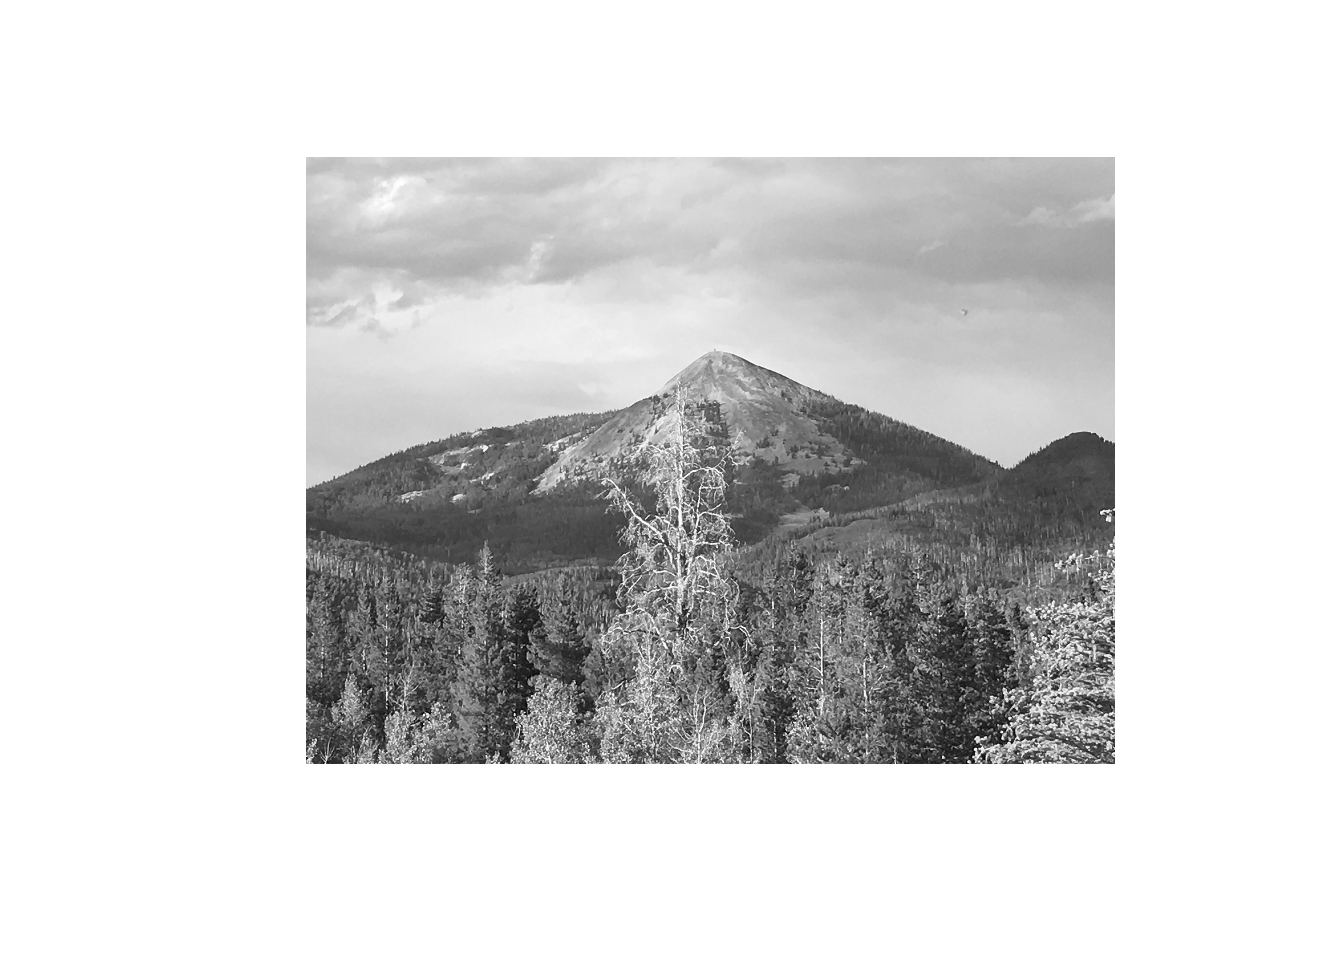
\includegraphics{_main_files/figure-latex/hahns-1.pdf}
\caption{\label{fig:hahns}Hahns Peak (author photo)}
\end{figure}

Here are the first ten rows and five columns of that matrix.

\begin{verbatim}
           [,1]      [,2]      [,3]      [,4]      [,5]
 [1,] 0.8236078 0.8196863 0.8157647 0.8118431 0.8040000
 [2,] 0.8196863 0.8196863 0.8157647 0.8079216 0.8040000
 [3,] 0.8157647 0.8157647 0.8118431 0.8079216 0.8040000
 [4,] 0.8118431 0.8079216 0.8079216 0.8040000 0.8000784
 [5,] 0.8040000 0.8040000 0.8040000 0.8000784 0.7961569
 [6,] 0.8000784 0.8000784 0.8000784 0.7961569 0.7961569
 [7,] 0.7961569 0.7961569 0.7961569 0.7922353 0.7922353
 [8,] 0.7961569 0.7922353 0.7922353 0.7922353 0.7922353
 [9,] 0.7922353 0.7883137 0.7804706 0.7765490 0.7726275
[10,] 0.7883137 0.7843922 0.7804706 0.7765490 0.7726275
\end{verbatim}

Before we do any fancy things with these matrices, we need to start with the basics. We need to talk about systems of equations.

\section{Systems of Equations}\label{systems-of-equations}

The simplest example of a system of linear equations\index{System of linear equations} is a system of two equations and two variables, such as

\begin{equation}
\left\{ 
\begin{array}{ccl}
x+y&=&150\\
    12x+6y&=&1500
\end{array}\right. .
\label{eq:2b2}
\end{equation}

This system of equations is \emph{linear} because both equations in the system are linear. A \emph{solution} to the system of equations is an \((x,y)\)-pair that satisfies both equations.

\subsection*{The geometry}\label{the-geometry}
\addcontentsline{toc}{subsection}{The geometry}

A single linear equation in two variables has a line as its graph. A linear system of two equations in two variables involves two lines (Fig. \ref{fig:intersecting}).

\begin{figure}

{\centering 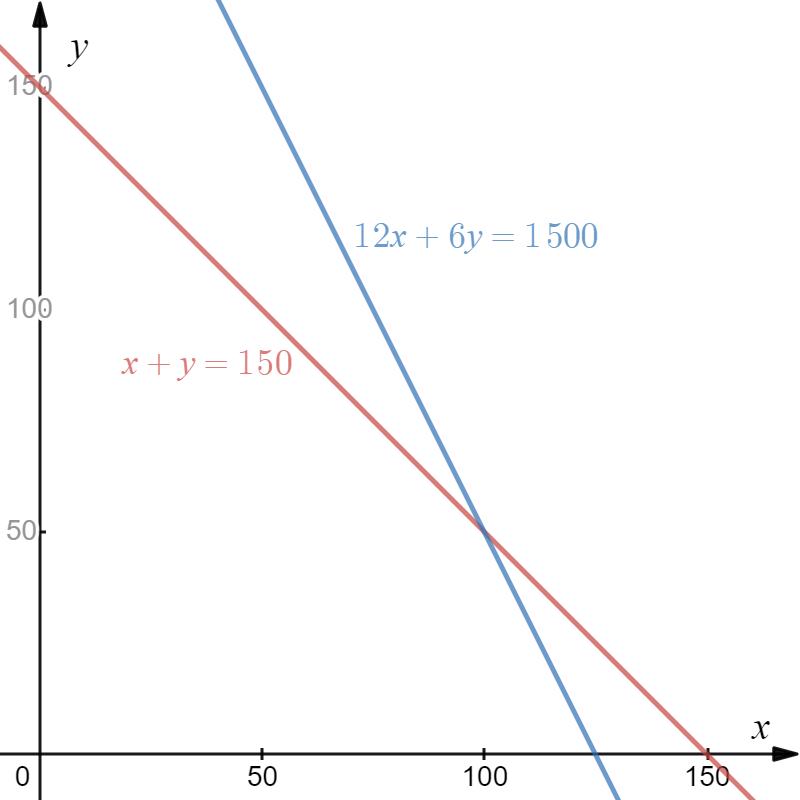
\includegraphics[width=0.5\linewidth]{images/soe1} 

}

\caption{Two intersecting lines}\label{fig:intersecting}
\end{figure}

A solution to the system must lie on both lines. In this case, it is the point of intersection.

Not all systems of two linear equations in two variables have a solution. If the two lines are parallel, there is no solution (Fig. \ref{fig:parallel}). Such systems are called \emph{inconsistent}\index{Inconsistent system}. (A system with a solution is \emph{consistent}\index{Consistent system}.)

\begin{figure}

{\centering 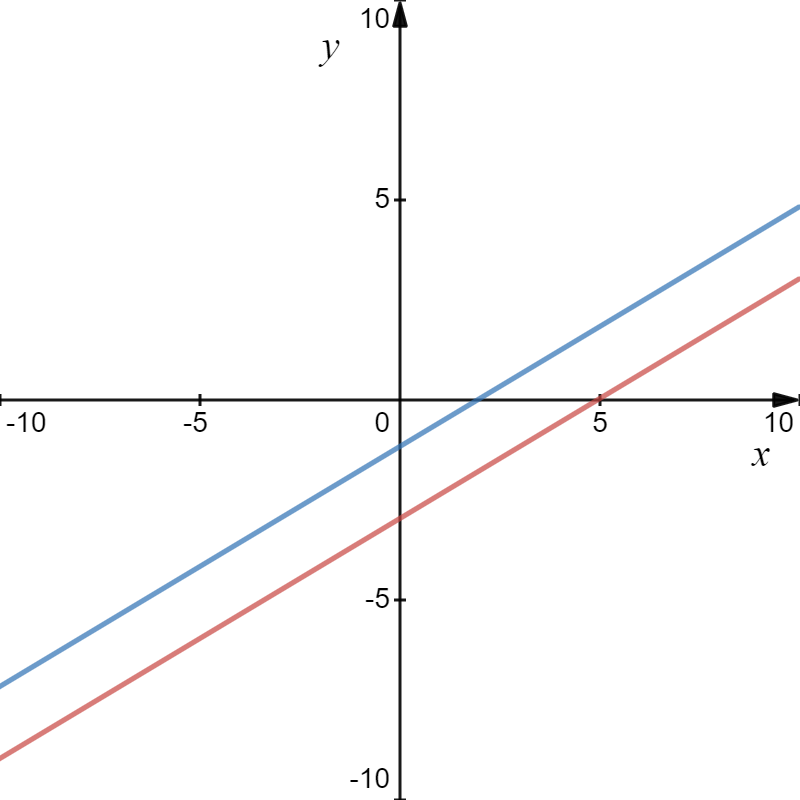
\includegraphics[width=0.5\linewidth]{images/soe2} 

}

\caption{Two parallel lines}\label{fig:parallel}
\end{figure}

Sometimes the two equations actually represent the same line. In that case the system is called \emph{dependent}\index{Dependent system} (Fig. \ref{fig:dependent}). Since every point on the line is a solution to both equations, we have infinitely many solutions.

\begin{figure}

{\centering 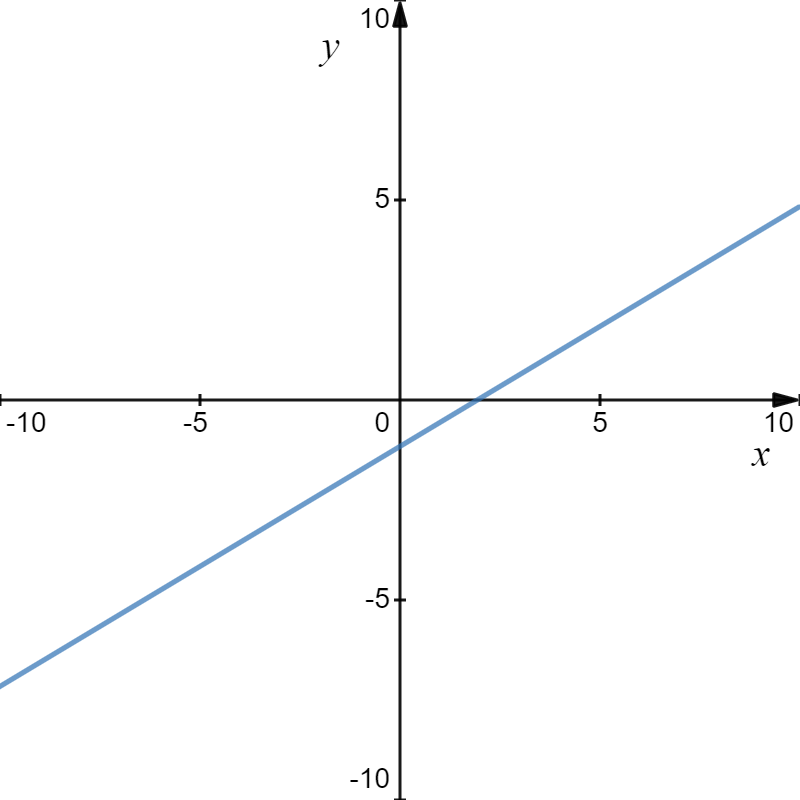
\includegraphics[width=0.5\linewidth]{images/soe3} 

}

\caption{Two equations, one line}\label{fig:dependent}
\end{figure}

\subsection*{The three cases}\label{the-three-cases}
\addcontentsline{toc}{subsection}{The three cases}

With a system of two linear equations in two variables, there are three possibilities.

\begin{enumerate}
\def\labelenumi{\arabic{enumi}.}
\tightlist
\item
  Exactly one solution (intersecting lines)
\item
  Infinitely many solutions (just one line)
\item
  No solutions (parallel lines)
\end{enumerate}

It turns out, when we increase the number of variables and/or equations, there are still these three possibilities for the number of solutions.

\section{Method of Solution: Gaussian Elimination}\label{GE}

Let's return to our original system of equations and try to solve it.

\begin{equation*}
\left\{ 
\begin{array}{ccl}
x+y&=&150\\
    12x+6y&=&1500
\end{array}\right. .
\end{equation*}

The method of \emph{Gaussian elimination}\index{Gaussian elimination} involves getting the system into a form that looks like this.

\begin{equation*}
\left\{ 
\begin{array}{rcl}
*x+*y & = &* \\
    *y & = & *
\end{array}\right. ,
\end{equation*}

where the asterisks represent different constants. If we have it in this \emph{upper triangular form}, we can immediately solve for \(y\), and once we know \(y\), we can use its value the first equation to solve for \(x\).

We can put a system of equations into upper triangular form using a sequence of operations on the equations. The following operations do not change the solution set for a linear system.

\begin{enumerate}
\def\labelenumi{\arabic{enumi}.}
\tightlist
\item
  Multiplying both sides of an equation by a nonzero constant
\item
  Adding a multiple of one equation to another (on both sides)
\item
  Rearranging the order of equations
\end{enumerate}

Once the system is in upper triangular form, we can use \emph{back substitution} to solve for all the variables. In the system

\begin{equation*}
\left\{ 
\begin{array}{ccl}
x+y&=&150\\
    12x+6y&=&1500
\end{array}\right. 
\end{equation*}

we want to turn the \(x\) coefficient in the second equation into a \(0\). We can do this by multiplying the first equation by \(-12\) and adding it to the second one. \emph{Note that we keep the first equation as is.} This puts us into upper triangular form.

\begin{equation*}
\left\{ 
\begin{array}{ccl}
x+y&=&150\\
    -6y&=&-300
\end{array}\right. \label{eq:utf}
\end{equation*}

We can now solve for \(y: y=\frac{-300}{-6}=50\). Plugging this value in for \(y\) in the first equation gives us \(x+50=150\) or \(x=100\). Our solution is \((x,y)=(100,50).\) Refer back to Figure \ref{fig:intersecting} for the geometry.

Let's verify that \((x,y)=(100,50)\) satisfies the original system \eqref{eq:2b2}. For the first equation,

\[x+y=100+50=150\,\checkmark\]

For the second equation,

\[12x+6y=12\cdot 100+6\cdot 50=1200+300=1500\,\checkmark\]

\begin{examplebox}

\begin{example}
Solve

\begin{equation*}
\left\{
\begin{array}{ccl}
x+2y&=&3\\
    2x-3y&=&10
\end{array}\right. .
\end{equation*}

If we add \(-2\) times the first equation to the second, we get

\begin{equation*}
\left\{
\begin{array}{rcl}
x+2y&=&3\\
    -7y&=&4
\end{array}\right. .
\end{equation*}

Thus, \(y=-4/7\) and \(x=3-2\left(-\frac{4}{7}\right)=\frac{21}{7}+\frac{8}{7}=\frac{29}{7}.\) Our solution is \(\left(-\frac{4}{7},\frac{29}{7}\right).\)
\end{example}

\end{examplebox}

What could go wrong?

\begin{examplebox}

\begin{example}
Solve

\begin{equation*}
\left\{
\begin{array}{ccl}
2x+3y&=&6\\
    4x+6y&=&7
\end{array}\right. .
\end{equation*}

If we multiply the top equation by \(-2\) and add it to the second, we get

\begin{equation*}
\left\{
\begin{array}{ccl}
2x+3y&=&6\\
    0x+0y&=&-5
\end{array}\right. .
\end{equation*}

Since \(0\neq -5\), this equation has no solution, i.e.~it is inconsistent. The original lines were parallel.
\end{example}

\end{examplebox}

What else could we encounter?

\begin{examplebox}

\begin{example}

If we tweak the last system a little bit\ldots{}

\begin{equation*}
\left\{
\begin{array}{ccl}
2x+3y&=&6\\
    4x+6y&=&12
\end{array}\right. ,
\end{equation*}

we see that by multiplying the top equation by 2 gives us identical equations. So

\begin{itemize}
\tightlist
\item
  the two equations represent the same line, and
\item
  every point on that line is a solution, and
\item
  there are infinitely many solutions.
\end{itemize}

\end{example}

\end{examplebox}

\subsection*{Parameters}\label{parameters}
\addcontentsline{toc}{subsection}{Parameters}

When a system of equation has infinitely many solutions, we like to write the solutions in terms of \emph{parameters}\index{Parameters}. For instance, in the last example, whose solution was the line \(2x+3y=6\), we can let \(y=t\) and solve for \(x\): \(2x+3t=6\) or \(x=3-\frac{3}{2}t\), and our solution is

\[\left\{(3-\frac{3}{2}t,t),t\in \mathbb{R}\right\}.\]

The last expression can be read as ``the set of all ordered pairs of the form \((3-\frac{3}{2}t,t)\), where \(t\) is an element of the real numbers.'' Different values of \(t\) lead to different solutions. For instance. if \(t=0,\) we have \((x,y)=(3,0),\) while if \(t=1,\) we get \((x,y)=\left(\frac{3}{2},1\right).\) Note that we can use any real number for \(t,\) not just an integer.

Parameterizations\index{Parameterization} are not unique. Letting \(x=t\) and solving for \(y\) gives us a different-looking solution:

\[\left\{(t,2-\frac{2}{3}t),t\in \mathbb{R}\right\}.\]

In the next section, we will learn a systematic way to parameterize solutions.

\subsection*{More equations, more variables}\label{more-equations-more-variables}
\addcontentsline{toc}{subsection}{More equations, more variables}

Here's a system of three linear equations in three variables.

\begin{examplebox}

\begin{example}
\protect\hypertarget{exm:tbt}{}\label{exm:tbt}Solve

\begin{equation*}
    \left\{
    \begin{array}{ccl}
    2x-2y+z&=&12\\
    x+y-2z&=&-1\\
    3x+y+2z&=&15 
    \end{array} \right. .
\end{equation*}

A single linear equation of the form

\[ax+by+cz=d,\]

where \(a,b,\) and \(c\) are constants (and not all zero), represents a plane in three dimensions. A solution to this system of equations would lie on the intersection of three planes. Again, the possibilities are zero, one, or infinitely many solutions.

We can again use Gaussian elimination to get the system into upper triangular form. It works best if the \(x\)-coefficient in the first equation is a 1.

If we interchange the first and second equations, we make that happen.

\begin{equation*}
    \left\{
    \begin{array}{ccl}
    x+y-2z&=&-1\\
    2x-2y+z&=&12\\
    3x+y+2z&=&15 
    \end{array} \right. .
\end{equation*}

We can use the \(x\) term in the first equation as a \emph{pivot}\index{Pivot} to eliminate the \(x\) term from the other two equations.

Replace Equation 2 with \(-2\times\) Equation 1 + Equation 2 (\(-2E1+E2\to E2\)), and replace Equation 3 with \(-3\times\) Equation 1 + Equation 3 (\(-3E1+E3\to E3\)).

\begin{equation*}
    \left\{
    \begin{array}{rcl}
    x+y-2z&=&-1\\
    -4y+5z&=&14\\
    -2y+8z&=&18 
    \end{array} \right. .
\end{equation*}

Let's divide Equation 3 by \(-2\) and then interchange Equations 2 and 3. (-\(\frac{1}{2}E3\to E3,E2\leftrightarrow E3\).)

\begin{equation*}
    \left\{
    \begin{array}{rcl}
    x+y-2z&=&-1\\
    y-4z&=&-9\\ 
    -4y+5z&=&14
    \end{array} \right. .
\end{equation*}

Now we'll use the \(y\) in Equation 2 as a pivot to eliminate the \(y\) term in Equation 3. \((4E2+E3\to E3.)\)

\begin{equation*}
    \left\{
    \begin{array}{rcl}
    x+y-2z&=&-1\\
    y-4z&=&-9\\ 
    -11z&=&-22
    \end{array} \right. .
\end{equation*}

We are now in triangular form, and we can solve immediately for \(z\): \(z=2\). We can use it in the second equation to solve for \(y\): \(y-4(2)=-9, y=-1\). Finally, knowing the values of \(y\) and \(z\) allows us to use Equation 1 to solve for \(x\): \(x+(-1)-2(2)=-1\) or \(x=4.\) Our solution is \((x,y,z)=(4,-1,2)\).
\end{example}

\end{examplebox}

What would a no-solution case look like? After Gaussian elimination, perhaps we end up with something like this:

\begin{examplebox}

\begin{example}
\begin{equation*}
    \left\{
    \begin{array}{rcl}
    x+2y+4z&=&2\\
    y-3z&=&1\\ 
    0&=&7
    \end{array} \right. .
\end{equation*}

Similar to the ``\(2\times 2\)'' case, a bottom row with \(0=a\), where \(a\neq 0\) would indicate an inconsistent system.
\end{example}

\end{examplebox}

\begin{examplebox}

\begin{example}
By tweaking the last example just a bit, we can arrive at a case with infinitely many solutions.

\begin{equation*}
    \left\{
    \begin{array}{rcl}
    x+2y+4z&=&2\\
    y-3z&=&1\\ 
    0&=&0
    \end{array} \right. .
\end{equation*}

The last equation is no longer a problem, but now we basically have more equations than unknowns. Again, we'll use a parameter. Let \(z=t\). Then \(y-3t=1\) or \(y=1+3t\). Also, \(x+2(1+3t)+4t=2\), which leads to \(x=-10t\). We write the solution as

\[\left\{(-10t,1+3t,t),t\in\mathbb{R}\right\}.\]

Again, this parameterization is not unique. Because there is a single parameter, our solution is a line in 3 dimensions.
\end{example}

\end{examplebox}

\begin{examplebox}

\begin{example}
\protect\hypertarget{exm:tfv}{}\label{exm:tfv}It is also possible after Gaussian elimination to end up with a system that looks like this.

\begin{equation*}
    \left\{
    \begin{array}{rcl}
    x+4y-3z&=&2\\
    0&=&0\\
    0&=&0
    \end{array} \right. 
\end{equation*}

That is, the three equations actually represent the same plane. In this case we use two parameters, \(s\) and \(t\) and solve for the third in terms of them. With \(y=s\) and \(z=t\), we get \(x=2-4y+3z=2-4s+3t\). Our solution is

\[\left\{(2-4s+3t,s,t),(s,t)\in \mathbb{R}^2\right\}.\]
\end{example}

\end{examplebox}

\subsection*{Overdetermined and underdetermined systems}\label{overdetermined-and-underdetermined-systems}
\addcontentsline{toc}{subsection}{Overdetermined and underdetermined systems}

We don't have to have the same number of equations as variables. When we have more equations than variables, the system is called \emph{overdetermined}\index{Overdetermined system}. For example,

\begin{equation*}
    \left\{
    \begin{array}{ccl}
    x+2y&=&3\\
    2x-y&=&5\\
    3x+y&=&8 \end{array} \right.
\end{equation*}

has three equations but only two unknowns. Though the system does have a single solution (left as an exercise), overdetermined systems often have no solution. They show up in linear regression and in other cases where there are more observations than there are variables.

\emph{Underdetermined}\index{Underdetermined system} systems have more variables than equations. For instance,

\begin{equation*}
    \left\{ \begin{array}{rcl}
    x+2y-3z&=&1\\
    y+2z&=&4 \end{array} \right. 
\end{equation*}

is underdetermined. Underdetermined systems don't have to have a solution, but if there's one solution, there are infinitely many. Why?

\section{Matrices}\label{matrices}

A \emph{matrix}\index{Matrix} is a rectangular array of numbers. Matrices can be used to store the coefficients in a system of equations. For instance, this system we saw in the last section,

\begin{equation*}
\left\{ 
\begin{array}{rcl}
2x-2y+z&=&12\\
    x+y-2z&=&-1\\
    3x+y+2z&=&15
\end{array}\right. 
\end{equation*}

can be written

\[\left[\begin{array}{rrr|r}
2&-2&1&12\\
1 & 1 & -2 & -1\\
3 & 1 & 2 & 15
\end{array}\right].\]

This is what we call an \emph{augmented matrix}\index{Augmented matrix}, with the constants separated from the coefficients by a vertical line. The \emph{coefficient matrix}\index{Coefficient matrix} is the matrix to the left of the line. We will be studying important properties of the coefficient matrix in the future.

\subsection*{Elementary row operations}\label{elementary-row-operations}
\addcontentsline{toc}{subsection}{Elementary row operations}

The three operations on systems of equations from the previous section have matrix equivalents, called \emph{elementary row operations}\index{Elementary row operations}. They are as follows.

\begin{enumerate}
\def\labelenumi{\arabic{enumi}.}
\tightlist
\item
  Interchanging two rows
\item
  Multiplying a row by a nonzero constant
\item
  Adding a constant multiple of one row to another
\end{enumerate}

We can use these three operations to solve a system of equations. (We are basically doing Gaussian elimination, but we're not writing down the variables all the time.)

\begin{examplebox}

\begin{example}
Solve using matrices:

\[ \left\{ \begin{array}{rcl}
y-4z&=&8\\
    2x-3y+2z&=&1\\
    4x-8y+12z&=&1 \end{array} \right. \]

The augmented matrix is

\[\left[\begin{array}{rrr|r}
0&1&-4&8\\
2 & -3 & 2 & 1\\
4 & -8 & 12 & 1
\end{array}\right].\]

Here is one possible sequence of steps.

\[\left[\begin{array}{rrr|r}
0&1&-4&8\\
2 & -3 & 2 & 1\\
4 & -8 & 12 & 1
\end{array}\right] \xrightarrow{R1\leftrightarrow R2} 
\left[\begin{array}{rrr|r}
2 & -3 & 2 & 1\\
0 & 1 & -4 & 8\\
4 & -8 & 12 & 1
\end{array}\right]\]

\[\xrightarrow{-2R1+R3\to R3}
\left[\begin{array}{rrr|r}
2 & -3 & 2 & 1\\
0 & 1 & -4 & 8 \\
0 & -2 & 8 & -1
\end{array}\right]\xrightarrow{2R2+R3\to R3}
\left[\begin{array}{rrr|r}
2 & -3 & 2 & 1\\
0 & 1 & -4 & 8 \\
0 & 0 & 0 & 15
\end{array}\right].
\]

The last line in the last matrix is equivalent to the equation \(0=15\). The system has no solution. (It is inconsistent.)
\end{example}

\end{examplebox}

\subsection*{Row echelon form}\label{row-echelon-form}
\addcontentsline{toc}{subsection}{Row echelon form}

Let's do one last thing to the final matrix in the last example.

\[\left[\begin{array}{rrr|r}
2 & -3 & 2 & 1\\
0 & 1 & -4 & 8 \\
0 & 0 & 0 & 15
\end{array}\right] \xrightarrow[\frac{1}{15}R3\to R3]{\frac{1}{2}R1\to R1}
\left[\begin{array}{rrr|r}
1 & -\frac32 & 1 & \frac12 \\
0 & 1 & -4 & 8 \\
0 & 0 & 0 & 1
\end{array}\right]
\]

This new matrix satisfies the following properties.

\begin{enumerate}
\def\labelenumi{\arabic{enumi}.}
\tightlist
\item
  All rows consisting entirely of zeros (if any) are at the bottom.
\item
  The first nonzero entry in each row is 1. This first nonzero entry is called the \emph{leading} 1.
\item
  Each leading 1 appears to the right of the leading 1 in any row above it.
\end{enumerate}

A matrix satisfying these three properties is said to be in \emph{row echelon form}\index{Row echelon form}. (Note: not everyone requires the first nonzero term in each row to be a 1.) Gaussian elimination on a matrix will leave it in row echelon form.

\subsection*{Reduced row echelon form}\label{reduced-row-echelon-form}
\addcontentsline{toc}{subsection}{Reduced row echelon form}

In the process of solving this system in Example \ref{exm:tbt}

\begin{equation*}
    \left\{
    \begin{array}{ccl}
    2x-2y+z&=&12\\
    x+y-2z&=&-1\\
    3x+y+2z&=&15 
    \end{array} \right. ,
\end{equation*}

we reduced it to this

\begin{equation*}
    \left\{
    \begin{array}{rcl}
    x+y-2z&=&-1\\
    y-4z&=&-9\\ 
    -11z&=&-22
    \end{array} \right. ,
\end{equation*}

which has row echelon matrix form

\[\left[\begin{array}{rrr|r}
1 & 1 & -2 & -1\\
0 & 1 & -4 & -9\\
0 & 0 & 1 & 2
\end{array}\right].\]

We used back substitution to solve the system, but we can also do more with the matrix:

\[\left[\begin{array}{rrr|r}
1 & 1 & -2 & -1\\
0 & 1 & -4 & -9\\
0 & 0 & 1 & 2
\end{array}\right]
\xrightarrow{-R2+R1\to R1}
\left[\begin{array}{rrr|r}
1 & 0 & 2 & 8\\
0 & 1 & -4 & -9\\
0 & 0 & 1 & 2
\end{array}\right]\]

\[\xrightarrow[4R3+R2\to R2]{-2R3+R1\to R1}
\left[\begin{array}{rrr|r}
1 & 0 & 0 & 4\\
0 & 1 & 0 & -1\\
0 & 0 & 1 & 2
\end{array}\right].
\]

We can immediately read off the solution to the system without having to back substitute: \(x=4,y=-1,z=2\). This matrix is in what we call \emph{reduced row echelon form}\index{Row echelon form!reduced}.

A matrix is in reduced row echelon form if it is in row echelon form and each leading 1 is the only nonzero entry in its column. (Note: while not everyone requires leading ones in \emph{row echelon form}, the standard definition of \emph{reduced row echelon form} does require them.) The reduced row echelon form of a matrix is unique. The process used to put a matrix into reduced row echelon form is called \emph{Gauss-Jordan elimination}\index{Gauss-Jordan elimination}.

Most graphing calculators can put matrices into reduced row echelon form. In the future, we will learn how to do it with R.

\begin{examplebox}

\begin{example}
Which of the following augmented matrices are in reduced row echelon form?

\[\mathbf{A}=\left[\begin{array}{rrrr|r}
1 & 0 & 0 & 0 & 2\\
0 & 1 & 0 & 0 & 3\\
0 & 0 & 1 & 0 & -2\\
0 & 0 & 0 & 1 & -3\end{array}\right] \]

\[\mathbf{B}=\left[\begin{array}{rrrr|r}
1 & 0 & 3 & 0 & 2\\
0 & 1 & 2 & 0 & 3\\
0 & 0 & 0 & 1 & -2\\
0 & 0 & 0 & 0 & 0\end{array}\right] \]

\[\mathbf{C}=\left[\begin{array}{rrr|r}
1 & 1 & 0 &  2\\
0 & 1 & 0 &  3\\
0 & 0 &  1 &  -2\end{array}\right] \]

\[\mathbf{D}=\left[\begin{array}{rrr|r}
1 & 0 & 1 & 3\\
0 & 1 & 1 & 2\end{array}\right] \]

Only matrix \(\mathbf{C}\) is not in reduced row echelon form. The leading 1 in the second row has a nonzero value above it. In the second matrix, the leading ones are in columns 1, 2, and 4.
\end{example}

\end{examplebox}

After using Gauss-Jordan elimination to get a matrix into reduced row echelon form, we can read the solution to the corresponding system of equations fairly easily. For instance (assuming the columns represent \(x,y,z,\) and \(w\), respectively), the system of equations corresponding to the first matrix in the last example

\[\left[\begin{array}{rrrr|r}
1 & 0 & 0 & 0 & 2\\
0 & 1 & 0 & 0 & 3\\
0 & 0 & 1 & 0 & -2\\
0 & 0 & 0 & 1 & -3\end{array}\right] \]

has the solution \(x=2,y=3,z=-2\), and \(w=-3\).

What about the solution to this one?

\[\left[\begin{array}{rrr|r}
1 & 0 & 1 & 3\\
0 & 1 & 1 & 2\end{array}\right] \]

Note that there is no leading 1 in the third column. Variables whose columns have no leading 1 are called \emph{free variables}\index{Free variable} and can actually take on any value. The rest of the solution depends on them. It's traditional to assign parameters to these free variables. Here \(z\) is free, so we let \(z=t\) and solve for the rest.

We use the second row to solve for \(y\):

\[y+z=2\to  y=2-z\to y=2-t\]

Similarly, we can use the first row to solve for \(x\):

\[x+z=3\to x=3-z\to x=3-t\]

Our solution is \(\{(3-t,2-t,t),t\in\mathbb{R}\}\).

It turns out that the reduced row echelon form of a matrix is unique, so our system of assigning parameters to the free variables gives us a systematic way of producing consistent parameterizations for solutions.

\begin{examplebox}

\begin{example}
This matrix also has a free variable.

\[\left[\begin{array}{rrrr|r}
1 & 0 & 3 & 0 & 2\\
0 & 1 & 2 & 0 & 3\\
0 & 0 & 0 & 1 & -2\\
0 & 0 & 0 & 0 & 0\end{array}\right] \]

If the variables are \(x,y,z\), and \(w\), then \(z\) is again a free variable. Let \(z=t\).
Note that \(w=-2\), regardless of the value of \(z\). We also get \(x=2-3z=2-3t\) and \(y=3-2z=3-2t\), so the general solution is

\[\{(2-3t,3-2t,t,-2),t\in\mathbb{R}\}\]

Another nice feature of this approach is that we can solve for the non-free or \emph{basic} variables\index{Basic variable} in terms of the free variables alone.
\end{example}

\end{examplebox}

\begin{examplebox}

\begin{example}
What if we have more than one free variable? We saw the following (reduced) system in Example \ref{exm:tfv}

\begin{equation*}
    \left\{
    \begin{array}{rcl}
    x+4y-3z&=&2\\
    0&=&0\\
    0&=&0
    \end{array} \right. 
\end{equation*}

The corresponding matrix is

\[\left[\begin{array}{rrr|r}
1 & 4 & -3 & 2\\
0 & 0 & 0 & 0\\
0 & 0 & 0 & 0
\end{array}\right].\]

Here, \(y\) and \(z\) are free variables. In this system, \(x\) is the only basic variable. If we let \(y=s\) and \(z=t\), we can solve for \(x\) and get the solution we saw before.
\end{example}

\end{examplebox}

\subsection*{Matrices with Technology}\label{TM}
\addcontentsline{toc}{subsection}{Matrices with Technology}

We use small-scale examples with nice solutions to illustrate the concepts, but in the real world, we use software packages to perform our computations.

For small matrices, the \href{https://www.desmos.com/matrix}{Desmos}\autocite{Desmos} matrix calculator is handy for basic matrix operations, and will even put a matrix in reduced row echelon form with the touch of the \texttt{rref} button.

In R, there are a few different ways to create a matrix. The \texttt{matrix} function is one of those ways.

\begin{Shaded}
\begin{Highlighting}[]
\NormalTok{M }\OtherTok{\textless{}{-}} \FunctionTok{matrix}\NormalTok{(}\FunctionTok{c}\NormalTok{(}\DecValTok{2}\NormalTok{,}\DecValTok{1}\NormalTok{,}\DecValTok{3}\NormalTok{,}\SpecialCharTok{{-}}\DecValTok{2}\NormalTok{,}\DecValTok{1}\NormalTok{,}\DecValTok{1}\NormalTok{,}\DecValTok{1}\NormalTok{,}\SpecialCharTok{{-}}\DecValTok{2}\NormalTok{,}\DecValTok{2}\NormalTok{,}\DecValTok{12}\NormalTok{,}\SpecialCharTok{{-}}\DecValTok{1}\NormalTok{,}\DecValTok{15}\NormalTok{), }\AttributeTok{nrow =} \DecValTok{3}\NormalTok{)}
\NormalTok{M}
\end{Highlighting}
\end{Shaded}

\begin{verbatim}
##      [,1] [,2] [,3] [,4]
## [1,]    2   -2    1   12
## [2,]    1    1   -2   -1
## [3,]    3    1    2   15
\end{verbatim}

We have created the augmented matrix that goes with Example \ref{exm:tbt}. (Note that neither Desmos nor R will display the augmentation bar. We just have to imagine it being there.) By default, when we feed the \texttt{matrix} function a vector (created by the \texttt{c} function), it will fill the matrix column-by-column. We specified the number of rows to be 3 with the \texttt{nrow\ =\ 3} argument, so when the first column fills up, the next 3 values go in column 2. If we want to enter the values by row, we can add a \texttt{byrow\ =\ TRUE} argument.

\begin{Shaded}
\begin{Highlighting}[]
\NormalTok{M2 }\OtherTok{\textless{}{-}} \FunctionTok{matrix}\NormalTok{(}\FunctionTok{c}\NormalTok{(}\DecValTok{2}\NormalTok{,}\DecValTok{1}\NormalTok{,}\DecValTok{3}\NormalTok{,}\SpecialCharTok{{-}}\DecValTok{2}\NormalTok{,}\DecValTok{1}\NormalTok{,}\DecValTok{1}\NormalTok{,}\DecValTok{1}\NormalTok{,}\SpecialCharTok{{-}}\DecValTok{2}\NormalTok{,}\DecValTok{2}\NormalTok{,}\DecValTok{12}\NormalTok{,}\SpecialCharTok{{-}}\DecValTok{1}\NormalTok{,}\DecValTok{15}\NormalTok{), }\AttributeTok{byrow =} \ConstantTok{TRUE}\NormalTok{,  }
              \AttributeTok{nrow =} \DecValTok{3}\NormalTok{)}
\NormalTok{M2}
\end{Highlighting}
\end{Shaded}

\begin{verbatim}
##      [,1] [,2] [,3] [,4]
## [1,]    2    1    3   -2
## [2,]    1    1    1   -2
## [3,]    2   12   -1   15
\end{verbatim}

To put a matrix into RREF form, we need the \texttt{rref} function from the \texttt{pracma} package.

\begin{Shaded}
\begin{Highlighting}[]
\FunctionTok{library}\NormalTok{(pracma)}
\FunctionTok{rref}\NormalTok{(M)}
\end{Highlighting}
\end{Shaded}

\begin{verbatim}
##      [,1] [,2] [,3] [,4]
## [1,]    1    0    0    4
## [2,]    0    1    0   -1
## [3,]    0    0    1    2
\end{verbatim}

With no free variables, we can read off our solution in the 4th column: \({(x,y,z)=(4,-1,2)}\).

\section{Basic Matrix Operations}\label{BMO}

So far, we've only used matrices as shorthand for an underlying linear system. It turns out that matrices have useful algebraic properties, which we will now study.

The \emph{dimension}\index{Dimension!of a matrix} or \emph{size} of a matrix is the number of rows and columns. An \(m\times n\) matrix has \(m\) rows (horizontal) and \(n\) columns (vertical). Here are some examples.

\begin{itemize}
\item
  \(\begin{bmatrix}
  2 & 3 & 2\\
  1 & 2 & 4
  \end{bmatrix} {\text{ is } 2\times 3}\)
\item
  \(\begin{bmatrix}
  -1 & 3 & 6 & 2\\
  2 & 1 & 0 & 0\\
  3 & 5 & 1 & 2
  \end{bmatrix}{\text{ is } 3\times 4}\)
\item
  \(\begin{bmatrix}
  2 & 1 \\
  1 & -2
  \end{bmatrix}{\text{ is } 2\times 2 \text{ (a } \textit{square matrix}\text{)}}\)
\end{itemize}

\subsection*{Row and column vectors}\label{row-and-column-vectors}
\addcontentsline{toc}{subsection}{Row and column vectors}

An \(m\times 1\) matrix is called a \emph{column vector}\index{Vector!column}.

\[\begin{bmatrix}
2\\4\\-1\\6\\7
\end{bmatrix} \]

A \(1\times n\) matrix is called a \emph{row vector}\index{Vector!row}.

\[\begin{bmatrix}
1 & 2 & -1 & 5 & 4 & 8
\end{bmatrix}\]

\subsection*{Matrix addition}\label{matrix-addition}
\addcontentsline{toc}{subsection}{Matrix addition}

Two matrices of the same dimension can be added together. The addition is entry-wise.
\begin{align*}
\begin{bmatrix}
2 & 4 & -1\\
3 & 2 & 3
\end{bmatrix}+
\begin{bmatrix}
4 & 2 & 1\\
2 & -2 & 3
\end{bmatrix}&=
\begin{bmatrix}
2+4 & 4+2 & -1+1\\
3+2 & 2+-2 & 3+3
\end{bmatrix}\\
&=
\begin{bmatrix}
6 & 6 & 0\\
5 & 0 & 6
\end{bmatrix}
\end{align*}

Matrix subtraction is similar. Again, the matrices must be of the same size.
\begin{align*}
\begin{bmatrix}
2 & 4 & -1\\
3 & 2 & 3
\end{bmatrix}-
\begin{bmatrix}
4 & 2 & 1\\
2 & -2 & 3
\end{bmatrix}&=
\begin{bmatrix}
2-4 & 4-2 & -1-1\\
3-2 & 2-(-2) & 3-3
\end{bmatrix}\\
&=
\begin{bmatrix}
-2 & 2 & -2\\
1 & 4 & 0
\end{bmatrix}
\end{align*}

\subsection*{Scalar Multiplication}\label{scalar-multiplication}
\addcontentsline{toc}{subsection}{Scalar Multiplication}

A matrix can be multiplied by a constant. This process is called \emph{scalar multiplication}\index{Multiplication!scalar} to avoid confusion with \emph{matrix multiplication}, which we will see in a bit. In scalar multiplication, each entry in the matrix is multiplied by the constant.

For instance

\[2\begin{bmatrix}
2 & 1\\-3 & 4
\end{bmatrix}=
\begin{bmatrix}
2\cdot 2 & 2\cdot 1\\ 2\cdot (-3) & 2\cdot 4
\end{bmatrix}=
\begin{bmatrix}
4 & 2\\-6 & 8
\end{bmatrix}.\]

The \emph{additive inverse} of a matrix \(\mathbf{A}\) is
\(-\mathbf{A}=(-1)\mathbf{A}\).

All of these operations are easily performed in Desmos and R. With \(\mathbf{M}\) and \(\mathbf{M2}\) from before, we get the following.

\begin{Shaded}
\begin{Highlighting}[]
\NormalTok{M}
\end{Highlighting}
\end{Shaded}

\begin{verbatim}
##      [,1] [,2] [,3] [,4]
## [1,]    2   -2    1   12
## [2,]    1    1   -2   -1
## [3,]    3    1    2   15
\end{verbatim}

\begin{Shaded}
\begin{Highlighting}[]
\NormalTok{M2}
\end{Highlighting}
\end{Shaded}

\begin{verbatim}
##      [,1] [,2] [,3] [,4]
## [1,]    2    1    3   -2
## [2,]    1    1    1   -2
## [3,]    2   12   -1   15
\end{verbatim}

\begin{Shaded}
\begin{Highlighting}[]
\NormalTok{M}\SpecialCharTok{+}\NormalTok{M2}
\end{Highlighting}
\end{Shaded}

\begin{verbatim}
##      [,1] [,2] [,3] [,4]
## [1,]    4   -1    4   10
## [2,]    2    2   -1   -3
## [3,]    5   13    1   30
\end{verbatim}

\begin{Shaded}
\begin{Highlighting}[]
\NormalTok{M}\SpecialCharTok{{-}}\NormalTok{M2}
\end{Highlighting}
\end{Shaded}

\begin{verbatim}
##      [,1] [,2] [,3] [,4]
## [1,]    0   -3   -2   14
## [2,]    0    0   -3    1
## [3,]    1  -11    3    0
\end{verbatim}

\begin{Shaded}
\begin{Highlighting}[]
\DecValTok{2}\SpecialCharTok{*}\NormalTok{M}
\end{Highlighting}
\end{Shaded}

\begin{verbatim}
##      [,1] [,2] [,3] [,4]
## [1,]    4   -4    2   24
## [2,]    2    2   -4   -2
## [3,]    6    2    4   30
\end{verbatim}

\begin{Shaded}
\begin{Highlighting}[]
\SpecialCharTok{{-}}\NormalTok{M}
\end{Highlighting}
\end{Shaded}

\begin{verbatim}
##      [,1] [,2] [,3] [,4]
## [1,]   -2    2   -1  -12
## [2,]   -1   -1    2    1
## [3,]   -3   -1   -2  -15
\end{verbatim}

Make sure to use the \texttt{*} for \emph{any} scalar multiplication.

The \(m\times n\) \emph{zero matrix} \(\mathbf{0}\) is the \(m\times n\) matrix with all zero entries. For instance, the \(2\times 3\) zero matrix is

\[\mathbf{0}=
\begin{bmatrix}
0 & 0 & 0\\0 & 0 & 0
\end{bmatrix}.\]

\begin{propbox}

\textbf{Properties of matrix arithmetic}

Let \(\mathbf{A}, \mathbf{B},\) and \(\mathbf{C}\) be any \(m\times n\) matrices, and let \(\mathbf{0}\) be the \(m\times n\) zero matrix. We have the following properties.

\begin{enumerate}
\def\labelenumi{\arabic{enumi}.}
\item
  Commutative property: \(\mathbf{A}+\mathbf{B}=\mathbf{B}+\mathbf{A}\)
\item
  Associative property: \(\mathbf{A}+(\mathbf{B}+\mathbf{C})=(\mathbf{A}+\mathbf{B})+\mathbf{C}\)
\item
  Identity property of addition: \(\mathbf{A}+\mathbf{0}=\mathbf{0}+\mathbf{A}=\mathbf{A}\)
\item
  Inverse property of addition: \(\mathbf{A}+(-\mathbf{A})=(-\mathbf{A})+\mathbf{A}=\mathbf{0}\)
\end{enumerate}

\end{propbox}

These properties follow from the analogous properties for real numbers.

\subsection*{Matrix multiplication}\label{matrix-multiplication}
\addcontentsline{toc}{subsection}{Matrix multiplication}

It would be simple to define the product of two matrices\index{Multiplication!matrix} in a similar manner. (In fact, the \texttt{*} operator in R does exactly that.) It turns out that a different definition is more useful for applications, but it will take a little motivation.

\begin{examplebox}

\begin{example}
A movie theater sold 200 tickets for a screening. Adult tickets cost \$12, senior tickets cost \$8, and children's tickets cost \$6 each. The theater received \$1,960 in revenue and sold 10 more senior tickets than children's tickets. How many of each type of ticket were sold?

Let \(x,y,\) and \(z\) represent the number of adult, senior, and children's tickets sold, respectively. There are three equations here.

\begin{itemize}
\tightlist
\item
  Tickets Sold: \(x+y+z=200\)
\item
  Revenue: \(12x+8y+6z=1960\)
\item
  Senior/child: \(y-z=10\)
\end{itemize}

The augmented matrix for the system and its reduced row echelon form look like this.

\[\left[\begin{array}{ccc|l} 1&1&1&200\\12 & 8 & 6 & 1960\\0 & 1 & -1 & 10\end{array}\right]\leadsto \left[\begin{array}{ccc|l} 1&0&0&110\\0 & 1 & 0 & 50\\0 & 0 & 1 & 40\end{array}\right].\]

The theater sold 110 adult tickets, 50 senior tickets, and 40 children's tickets. Let's store these numbers in a column vector.

\[\mathbf{v}=\begin{bmatrix} 110\\50\\40\end{bmatrix}\]

Let's look at the coefficient matrix, this solution vector, and the augmented vector together.

\[\begin{bmatrix}1&1&1\\12 & 8 & 6\\0 & 1 & -1 \end{bmatrix},\begin{bmatrix} 110\\50\\40\end{bmatrix},\text{ and }\begin{bmatrix} 200\\1960\\10\end{bmatrix}\]

We can get the revenue by combining the middle row and the solution vector:

\[\text{Revenue} = 12\cdot110+8\cdot 50+6\cdot 40=1960\]

\[\begin{bmatrix}&&\\12 & 8 & 6\\ &  &  \end{bmatrix},\begin{bmatrix} 110\\50\\40\end{bmatrix},\begin{bmatrix} \\1960\\ \\ \end{bmatrix}\]

You might recognize this as a \emph{dot product}\index{Dot product} of vectors:

\[(a_1,a_2,a_3)\cdot (b_1,b_2,b_3)=a_1b_1+a_2b_2+a_3b_3.\]

The total revenue, the second entry in the augmented vector is the dot product of the second row of the coefficient matrix and the solution vector. Similarly, the first entry (ticket sales) is the dot product of the first row and the solution vector, and the third entry is the dot product of the third row and the solution vector.

This is how we are going to define the product of a matrix and a vector.

\[\begin{bmatrix}1&1&1\\12 & 8 & 6\\0 & 1 & -1 \end{bmatrix}\begin{bmatrix} 110\\50\\40\end{bmatrix}=\begin{bmatrix} 200\\1960\\10\end{bmatrix}\]
\end{example}

\end{examplebox}

Here's an another example

\begin{examplebox}

\begin{example}
\[
\underbrace{\begin{bmatrix}
2 & 4 & 1 & 5\\ 
1 & -3 & 2 & 4\end{bmatrix}}_{2\times 4}\underbrace{\begin{bmatrix} 3 \\ -1 \\ 2 \\ 3
\end{bmatrix}}_{4\times 1}=\begin{bmatrix} 2\cdot 3+4\cdot (-1)+1\cdot 2+5\cdot 3\\ 1\cdot 3+(-3)\cdot (-1)+2\cdot 2+4\cdot 3
\end{bmatrix}
=\underbrace{\begin{bmatrix} 19\\22\end{bmatrix}}_{2\times 1}
\]
\end{example}

\end{examplebox}

\subsection*{Multiplying two matrices}\label{multiplying-two-matrices}
\addcontentsline{toc}{subsection}{Multiplying two matrices}

Having defined what it means to multiply a vector by a matrix, we can now talk about multiplying two matrices.

\[\underbrace{\begin{bmatrix}
2 & 4 & 1 & 5\\ 
1 & -3 & 2 & 4
\end{bmatrix}}_{2\times 4}
\underbrace{\begin{bmatrix}
1 & 2\\
-2 & 3\\
2 & 2\\
-1 & 4
\end{bmatrix}}_{4\times 2}=
\underbrace{
\begin{bmatrix}
-9 & 38 \\ 7 & 13\end{bmatrix}}_{2\times 2}\]

If \(\mathbf{A}\) is an \(m\times n\) matrix and \(\mathbf{B}\) is an \(n\times k\) matrix, then their product \(\mathbf{A}\mathbf{B}\) is an \(m\times k\) matrix whose \(i\)th column is the product of \(\mathbf{A}\) and the \(i\)th column of \(\mathbf{B}\).

The first column in the product is

\[\begin{bmatrix}
  2 & 4 & 1 & 5\\ 
  1 & -3 & 2 & 4
  \end{bmatrix}
  \begin{bmatrix}
  1 & *\\
  -2 & *\\
  2 & *\\
  -1 & *
    \end{bmatrix}=
    \begin{bmatrix}
  -9 & * \\ 7 & *\end{bmatrix}
  \]
and the second column is

\[\begin{bmatrix}
  2 & 4 & 1 & 5\\ 
  1 & -3 & 2 & 4
  \end{bmatrix}
  \begin{bmatrix}
  * & 2\\
  * & 3\\
  * & 2\\
  * & 4
  \end{bmatrix}=
    \begin{bmatrix}
  * & 38 \\ * & 13\end{bmatrix}.\]

\begin{examplebox}

\begin{example}
\protect\hypertarget{exm:twobytwo}{}\label{exm:twobytwo}Multiply

\[\begin{bmatrix} 2 & -1 \\ 3 & -2\end{bmatrix} \begin{bmatrix}1 & 2\\3 & 4\end{bmatrix}.\]

Let's introduce some notation. Suppose \(\mathbf{C}\) is an \(m\times n\) matrix. We denote the row \(i\), column \(j\) entry of \(\mathbf{C}\) by \(c_{ij}\). If \(\mathbf{C}=\mathbf{A}\mathbf{B}\), then \(c_{ij}\) is the dot product of row \(i\) of \(\mathbf{A}\) and column \(j\) of \(\mathbf{B}\).

The row 1, column 1 entry in our product is

\[\begin{bmatrix} 2 & -1 \\ * & *\end{bmatrix} \begin{bmatrix}1 & *\\3 & *\end{bmatrix}=\begin{bmatrix} 2\cdot 1+(-1)\cdot 3 & *\\ * & *\end{bmatrix}=\begin{bmatrix} -1 & *\\ * & *\end{bmatrix}\]

Pairing all of the other possible rows and columns gives us

\[\begin{bmatrix} 2 & -1 \\ 3 & -2\end{bmatrix} \begin{bmatrix}1 & 2\\3 & 4\end{bmatrix}=\begin{bmatrix}-1 & 0\\-3 & -2\end{bmatrix}\]
\end{example}

\end{examplebox}

You can't just multiply any pair of matrices. For example

\[\underbrace{\begin{bmatrix} 1 & 2 & 3\\2 & 4 & 1\end{bmatrix}}_{2\times 3}\underbrace{\begin{bmatrix} 2& 3\\1 & 4\end{bmatrix}}_{2\times 2}\]

doesn't work, because the number of columns on the left and the number of rows on the right don't match up.

What happens when we multiply the two matrices from Example \ref{exm:twobytwo}, but in the opposite order?

\[\begin{bmatrix}1 & 2\\3 & 4\end{bmatrix}
\begin{bmatrix} 2 & -1 \\ 3 & -2\end{bmatrix} =\begin{bmatrix}
8 & -5 \\18 & -11
\end{bmatrix}.\]

We get a different answer. Matrix multiplication is \textbf{not} commutative. In fact,

\[\begin{bmatrix}
1 & 2 & 1\\2 & 1 & 3\end{bmatrix} \begin{bmatrix}
1 & 2 & -1\\ 2 & 1 & 4 \\1 & -1 & -1
\end{bmatrix}=
\begin{bmatrix}
6 & 3 & 6\\7 & 2 & -1
\end{bmatrix},\]

but

\[\begin{bmatrix}
1 & 2 & -1\\ 2 & 1 & 4 \\1 & -1 & -1
\end{bmatrix}
\begin{bmatrix}
1 & 2 & 1\\2 & 1 & 3\end{bmatrix} \]

isn't even defined.

\begin{propbox}

\textbf{Properties of Matrix Multiplication}

If \(\mathbf{A},\mathbf{B},\) and \(\mathbf{C}\) are matrices such that all the indicated sums and products exist and \(r\) is a scalar, then the following properties are satisfied.

\begin{enumerate}
\def\labelenumi{\arabic{enumi}.}
\item
  Associative: \(\mathbf{A}(\mathbf{BC})=(\mathbf{AB})\mathbf{C}\)
\item
  Distributive:

  \begin{enumerate}
  \def\labelenumii{\alph{enumii}.}
  \item
    \(\mathbf{A}(\mathbf{B}+\mathbf{C})=\mathbf{AB}+\mathbf{AC}\)
  \item
    \((\mathbf{A}+\mathbf{B})\mathbf{C}=\mathbf{AC}+\mathbf{BC}\)
  \end{enumerate}
\item
  Scalar Commutativity: \(\mathbf{A}(r\mathbf{B})=r\mathbf{A}\mathbf{B}\)
\end{enumerate}

\end{propbox}

These properties are a little harder to prove, but note that associativity means that we can multiply three or more matrices by multiplying two at a time, and the pairing does not matter.

\subsection*{Identity Matrices}\label{identity-matrices}
\addcontentsline{toc}{subsection}{Identity Matrices}

The \emph{main diagonal}, or more simply, the \emph{diagonal}\index{Diagonal!of a matrix} of a square (\(n\times n\)) matrix \(\mathbf{A}\) are the entries of the form \(a_{ii}\). That is, they are the entries whose row and column indices match.

The diagonal of this matrix is highlighted.

\[\begin{bmatrix} \mathbf{3} & 2 & 1\\ 4 & \mathbf{-3} & 1\\4 & 2 & \mathbf{9}\end{bmatrix}\]

The \(n\times n\) \emph{identity matrix}\index{Identity matrix} \(\mathbf{I}\) has ones along its main diagonal and zeros everywhere else. For example

\begin{itemize}
\tightlist
\item
  \(2\times 2:\mathbf{I}=\displaystyle{\begin{bmatrix}
    1 & 0 \\0 & 1\end{bmatrix}}\)
\item
  \(3\times 3:\mathbf{I}=\displaystyle{\begin{bmatrix}
    1 & 0 & 0\\0 & 1 & 0\\0 & 0 & 1
    \end{bmatrix}}\)
\end{itemize}

If \(\mathbf{A}\) is any matrix, and \(\mathbf{I}\) is the appropriately sized identity matrix, then \(\mathbf{AI}=\mathbf{A}\). Similarly, \(\mathbf{IA}=\mathbf{A}\) for the appropriately sized \(\mathbf{I}.\)

For example,

\[\begin{bmatrix}
    1 & 0 \\0 & 1\end{bmatrix} \begin{bmatrix} 2 & 1 & 4\\3 & -2 & 6\end{bmatrix}=\begin{bmatrix} 2 & 1 & 4\\3 & -2 & 6\end{bmatrix}\]

and

\[\begin{bmatrix} 2 & 1 & 4\\3 & -2 & 6\end{bmatrix}\begin{bmatrix}
    1 & 0 & 0\\0 & 1 & 0\\0 & 0 & 1
    \end{bmatrix}=\begin{bmatrix} 2 & 1 & 4\\3 & -2 & 6\end{bmatrix}.\]

\subsection*{Technology}\label{technology}
\addcontentsline{toc}{subsection}{Technology}

In \href{https://www.desmos.com/matrix}{Desmos}, we can multiply matrices using \texttt{*}. (It will show a \(\cdot\)).

In R, we must use the \texttt{\%*\%} operator to perform matrix multiplication as we defined it. (As mentioned before, \texttt{*} will multiply the corresponding entries in the two matrices, which is useful for some things, but not for our purposes.)

\begin{Shaded}
\begin{Highlighting}[]
\NormalTok{A }\OtherTok{\textless{}{-}} \FunctionTok{matrix}\NormalTok{(}\FunctionTok{c}\NormalTok{(}\DecValTok{2}\NormalTok{,}\DecValTok{1}\NormalTok{,}\DecValTok{3}\NormalTok{,}\SpecialCharTok{{-}}\DecValTok{2}\NormalTok{,}\DecValTok{1}\NormalTok{,}\DecValTok{1}\NormalTok{,}\DecValTok{1}\NormalTok{,}\SpecialCharTok{{-}}\DecValTok{2}\NormalTok{,}\DecValTok{2}\NormalTok{), }\AttributeTok{nrow =} \DecValTok{3}\NormalTok{)}
\NormalTok{A}
\end{Highlighting}
\end{Shaded}

\begin{verbatim}
##      [,1] [,2] [,3]
## [1,]    2   -2    1
## [2,]    1    1   -2
## [3,]    3    1    2
\end{verbatim}

\begin{Shaded}
\begin{Highlighting}[]
\NormalTok{B }\OtherTok{\textless{}{-}} \FunctionTok{matrix}\NormalTok{(}\FunctionTok{c}\NormalTok{(}\DecValTok{1}\NormalTok{,}\DecValTok{2}\NormalTok{,}\DecValTok{3}\NormalTok{,}\DecValTok{5}\NormalTok{,}\DecValTok{1}\NormalTok{,}\DecValTok{2}\NormalTok{), }\AttributeTok{nrow =} \DecValTok{3}\NormalTok{)}
\NormalTok{B}
\end{Highlighting}
\end{Shaded}

\begin{verbatim}
##      [,1] [,2]
## [1,]    1    5
## [2,]    2    1
## [3,]    3    2
\end{verbatim}

\begin{Shaded}
\begin{Highlighting}[]
\NormalTok{A}\SpecialCharTok{\%*\%}\NormalTok{B}
\end{Highlighting}
\end{Shaded}

\begin{verbatim}
##      [,1] [,2]
## [1,]    1   10
## [2,]   -3    2
## [3,]   11   20
\end{verbatim}

\begin{Shaded}
\begin{Highlighting}[]
\NormalTok{B}\SpecialCharTok{\%*\%}\NormalTok{A}
\end{Highlighting}
\end{Shaded}

\begin{verbatim}
## Error in B %*% A: non-conformable arguments
\end{verbatim}

\subsection*{The transpose of a matrix}\label{the-transpose-of-a-matrix}
\addcontentsline{toc}{subsection}{The transpose of a matrix}

One operation on a matrix that will come in handy in the future is the \emph{transpose}.

\begin{defbox}

\begin{definition}
Let \(\mathbf{A}\) be an \(m\times n\) matrix. The \emph{transpose}\index{Transpose} of \(\mathbf{A}\), denoted \(\mathbf{A}^T,\) is the \(n\times m\) matrix whose rows are the columns of \(\mathbf{A}\) and whose columns are the rows of \(\mathbf{A}\).
\end{definition}

\end{defbox}

Here are some examples. If

\[\mathbf{A}=\begin{bmatrix} a & b\\c & d\end{bmatrix},\]

then

\[\mathbf{A}^T=\begin{bmatrix} a& c\\b& d\end{bmatrix}.\]

If
\[\mathbf{A}=\begin{bmatrix}1 & 2 & 3\\4 & 5 & 6\end{bmatrix},\]
then

\[\mathbf{A}^T=\begin{bmatrix} 1 & 4\\2 & 5\\3 & 6\end{bmatrix}.\]

\begin{propbox}

\textbf{Properties of the Transpose}

If \textbf{A} and \textbf{B} are matrices of compatible sizes, and \(c\) is a constant, then we have the following properties.

\begin{enumerate}
\def\labelenumi{\arabic{enumi}.}
\item
  \(\left(\textbf{A}^T\right)^T=\textbf{A}\)
\item
  \((\textbf{A}+\textbf{B})^T=\textbf{A}^T+\textbf{B}^T\)
\item
  \((c\textbf{A})^T=c\textbf{A}^T\)
\item
  \((\textbf{A}\textbf{B})^T=\textbf{B}^T\textbf{A}^T\)
\end{enumerate}

\end{propbox}

In R, the function \texttt{t} will take the transpose of a matrix.

\begin{Shaded}
\begin{Highlighting}[]
\NormalTok{B }\OtherTok{\textless{}{-}} \FunctionTok{matrix}\NormalTok{(}\FunctionTok{c}\NormalTok{(}\DecValTok{1}\NormalTok{,}\DecValTok{2}\NormalTok{,}\DecValTok{3}\NormalTok{,}\DecValTok{5}\NormalTok{,}\DecValTok{1}\NormalTok{,}\DecValTok{2}\NormalTok{), }\AttributeTok{nrow =} \DecValTok{3}\NormalTok{)}
\NormalTok{B}
\end{Highlighting}
\end{Shaded}

\begin{verbatim}
##      [,1] [,2]
## [1,]    1    5
## [2,]    2    1
## [3,]    3    2
\end{verbatim}

\begin{Shaded}
\begin{Highlighting}[]
\FunctionTok{t}\NormalTok{(B)}
\end{Highlighting}
\end{Shaded}

\begin{verbatim}
##      [,1] [,2] [,3]
## [1,]    1    2    3
## [2,]    5    1    2
\end{verbatim}

\section{Matrix Inverses}\label{Inverses}

An \(n\times n\) matrix \(\mathbf{A}\) is \emph{invertible}\index{Invertible matrix} if there is an \(n\times n\) matrix \(\mathbf{A}^{-1}\) such that

\[\mathbf{A}\mathbf{A}^{-1}=\mathbf{A}^{-1}\mathbf{A}=\mathbf{I}.\]

The matrix \(\mathbf{A}^{-1}\) is the \emph{inverse}\index{Inverse!of a matrix} of \(\mathbf{A}\).

For instance, if \(\displaystyle{\mathbf{A}=\begin{bmatrix}
2 & 1\\1 & 1
\end{bmatrix}}\) and \(\mathbf{B}=\displaystyle{\begin{bmatrix}
1 & -1\\-1 & 2
\end{bmatrix}},\) let's show that \(\mathbf{B}=\mathbf{A}^{-1}.\) We have

\[\mathbf{AB}=\begin{bmatrix}
2 & 1\\1 & 1
\end{bmatrix}\begin{bmatrix}
1 & -1\\-1 & 2
\end{bmatrix}=\begin{bmatrix}
1 & 0 \\0 & 1
\end{bmatrix}=\mathbf{I},\]

and

\[\mathbf{BA}=\begin{bmatrix}
1 & -1\\-1 & 2
\end{bmatrix}\begin{bmatrix}
2 & 1\\1 & 1
\end{bmatrix}=\begin{bmatrix}
1 & 0 \\0 & 1
\end{bmatrix}=\mathbf{I},\]

so \(\mathbf{B}=\mathbf{A}^{-1}\) (and \(\mathbf{A}=\mathbf{B}^{-1})\).

\subsection*{Finding inverses}\label{finding-inverses}
\addcontentsline{toc}{subsection}{Finding inverses}

We can find the inverse of a matrix \(\mathbf{A}\) by solving the matrix equation \(\mathbf{AX}=\mathbf{I}\). The way we do this is by row reduction with the matrix \(\mathbf{A}\) augmented by the columns of \(\mathbf{I}\).

For example, to find \(\mathbf{A}^{-1}\) for \(\mathbf{A}=\displaystyle{\begin{bmatrix}
2 & 1\\1 & 1
\end{bmatrix}}\), we row reduce

\[\left[\begin{array}{cc|cc}
2 & 1 & 1 & 0\\1 & 1 & 0 & 1
\end{array}\right].\]

\begin{align*}\left[\begin{array}{cc|cc}
2 & 1 & 1 & 0\\1 & 1 & 0 & 1
\end{array}\right]&\xrightarrow{R1\leftrightarrow R2}\left[\begin{array}{cc|cc}
1 & 1 & 0 & 1\\2 & 1 & 1 & 0
\end{array}\right] \xrightarrow{-2R1+R2\to R2} \left[\begin{array}{cc|cc}
     1& 1 & 0 & 1  \\
     0 & -1 & 1 & -2
\end{array}\right] \\
&\xrightarrow{-R2\to R2} \left[\begin{array}{cc|cc}
     1& 1 & 0 & 1  \\
     0 & 1 & -1 & 2
\end{array}\right] \xrightarrow{-R2+R1\to R1} 
\left[\begin{array}{rr|rr}
     1& 0 & 1 & -1  \\
     0 & 1 & -1 & 2
\end{array}\right]
\end{align*}

and our inverse is

\[\mathbf{A}^{-1}=\begin{bmatrix}
1 & -1\\-1 & 2
\end{bmatrix}.\]

\begin{examplebox}

\begin{example}
\protect\hypertarget{exm:3b3inv}{}\label{exm:3b3inv}Here's a \(3\times 3\) example, though we will skip the messy bit.

Find \(\mathbf{A}^{-1}\) if

\[\mathbf{A}=\begin{bmatrix} 1 & 2 & 3\\3 & 1 & 1\\1 & 4 & 5\end{bmatrix}.\]

We augment \(\mathbf{A}\) with the \(3\times 3\) identity matrix and reduce.

\[\left[\begin{array}{ccc|ccc} 1 & 2 & 3 & 1 & 0 & 0\\3 & 1 & 1 & 0 & 1 & 0\\1 & 4 & 5 & 0 & 0 & 1\end{array}\right] \leadsto \left[\begin{array}{ccc|ccc} 1 & 0 & 0 & \frac{1}{6} & \frac{1}{3} & -\frac{1}{6}\\0 & 1 & 0 & -\frac{7}{3} & \frac{1}{3} & \frac{4}{3} \\ 0 & 0 & 1 & \frac{11}{6} & -\frac{1}{3} & -\frac{5}{6}\end{array}\right]\]

Our inverse is

\[\mathbf{A}^{-1}=\begin{bmatrix}\frac{1}{6} & \frac{1}{3} & -\frac{1}{6}\\-\frac{7}{3} & \frac{1}{3} & \frac{4}{3} \\ \frac{11}{6} &-\frac{1}{3} & -\frac{5}{6}\end{bmatrix}.\]

They aren't always pretty.
\end{example}

\end{examplebox}

Not all square matrices have inverses. For instance, if \(\mathbf{A}=\displaystyle{\begin{bmatrix}
1 & 2\\ -2 & -4
\end{bmatrix}}\), when we try to find our inverse, we get

\[\left[\begin{array}{rr|rr}
    1 & 2 & 1 & 0\\
    -2 & -4 & 0 & 1
\end{array}\right]\xrightarrow{2R1+R2\to R2}
\left[\begin{array}{rr|rr}
    1 & 2 & 1 & 0  \\
    0 & 0 & 2 & 1
\end{array}\right]\]

and we're stuck. This matrix has no inverse. Noninvertible matrices are also called \emph{singular}. They play an important role in Linear Algebra.

\subsection*{A formula for 2 x 2 matrices}\label{a-formula-for-2-x-2-matrices}
\addcontentsline{toc}{subsection}{A formula for 2 x 2 matrices}

Using row reduction on the augmented matrix

\[\left[\mathbf{A}|\mathbf{I}\right]=\left[\begin{array}{rr|rr}
a & b & 1 & 0\\ c & d & 0 & 1
\end{array}\right] \]

leads to the following formula for \(\mathbf{A}^{-1}\). We'll state it as our first theorem.

\begin{theorembox}

\begin{theorem}
\protect\hypertarget{thm:2b2invthm}{}\label{thm:2b2invthm}If \(\mathbf{A}=\displaystyle{\begin{bmatrix}a & b\\c & d\end{bmatrix}}\) and \(ad-bc\neq 0\), then \(\mathbf{A}\) is invertible and

\[\mathbf{A}^{-1}=\frac{1}{ad-bc}\begin{bmatrix}
d & -b\\-c & a
\end{bmatrix}.\label{eq:2b2inv}\]
\end{theorem}

\end{theorembox}

This result is very handy. Here are some examples.

\begin{examplebox}

\begin{example}
Let \(\mathbf{A}=\displaystyle{\begin{bmatrix}
2 & -1 \\ 3 & 4
\end{bmatrix}}.\)

Then

\[\mathbf{A}^{-1}=\frac{1}{2\cdot 4-(-1)\cdot 3}\begin{bmatrix}
4 & 1\\-3 & 2
\end{bmatrix}=\frac{1}{11}\begin{bmatrix}
4 & 1\\-3 & 2
\end{bmatrix}=\begin{bmatrix}
\frac{4}{11} & \frac{1}{11}\\ -\frac{3}{11} & \frac{2}{11}
\end{bmatrix}.\]
\end{example}

\end{examplebox}

\begin{examplebox}

\begin{example}
If \(\mathbf{B}=\displaystyle{\begin{bmatrix}
2 & 3\\6 & 9
\end{bmatrix}},\)

then

\[\mathbf{B}^{-1}=\frac{1}{2\cdot 9-6\cdot 3}\begin{bmatrix}
9 & -3 \\ -6 & 2
\end{bmatrix}=\frac{1}{0}\begin{bmatrix}
9 & -3 \\ -6 & 2
\end{bmatrix}\dots\]

This matrix is not invertible. Note that the second row of \(\mathbf{B}\) is a multiple of the first row. The second column is also a multiple of the first column. For singular \(2\times 2\) matrices, this is always the case. It's more complicated for bigger matrices.
\end{example}

\end{examplebox}

Speaking of larger matrices, there is a general formula for the inverse of an \(n\times n\) matrix, but it involves concepts that we are not going to get to. You might see it in a higher level Linear Algebra or Matrix Algebra course.

As is usually the case, most of the time we will be using technology to find inverses. Desmos has an inverse matrix button. In R, we use the multipurpose \texttt{solve} function.

\begin{Shaded}
\begin{Highlighting}[]
\NormalTok{A }\OtherTok{\textless{}{-}} \FunctionTok{matrix}\NormalTok{(}\FunctionTok{c}\NormalTok{(}\DecValTok{2}\NormalTok{,}\DecValTok{1}\NormalTok{,}\DecValTok{3}\NormalTok{,}\SpecialCharTok{{-}}\DecValTok{2}\NormalTok{,}\DecValTok{1}\NormalTok{,}\DecValTok{1}\NormalTok{,}\DecValTok{1}\NormalTok{,}\SpecialCharTok{{-}}\DecValTok{2}\NormalTok{,}\DecValTok{2}\NormalTok{), }\AttributeTok{nrow =} \DecValTok{3}\NormalTok{)}
\NormalTok{A}
\end{Highlighting}
\end{Shaded}

\begin{verbatim}
##      [,1] [,2] [,3]
## [1,]    2   -2    1
## [2,]    1    1   -2
## [3,]    3    1    2
\end{verbatim}

\begin{Shaded}
\begin{Highlighting}[]
\FunctionTok{solve}\NormalTok{(A)}
\end{Highlighting}
\end{Shaded}

\begin{verbatim}
##             [,1]        [,2]      [,3]
## [1,]  0.18181818  0.22727273 0.1363636
## [2,] -0.36363636  0.04545455 0.2272727
## [3,] -0.09090909 -0.36363636 0.1818182
\end{verbatim}

The following properties of are helpful.

\begin{propbox}

\textbf{Properties of matrix inverses}

Let \(\mathbf{A}\) and \(\mathbf{B}\) be invertible \(n\times n\) matrices. Then

\begin{enumerate}
\def\labelenumi{\arabic{enumi}.}
\item
  \(\mathbf{A}^{-1}\) is invertible and \((\mathbf{A}^{-1})^{-1}=\mathbf{A}.\)
\item
  \(\mathbf{A}\mathbf{B}\) is invertible and \((\mathbf{A}\mathbf{B})^{-1}=\mathbf{B}^{-1}\mathbf{A}^{-1}\).
\end{enumerate}

\end{propbox}

Property 2 is easy to prove. For instance,

\[(\mathbf{AB})(\mathbf{B}^{-1}\mathbf{A}^{-1})=\mathbf{A}(\mathbf{B}\mathbf{B}^{-1})\mathbf{A}^{-1}=\mathbf{A}\mathbf{I}\mathbf{A}^{-1}=\mathbf{A}\mathbf{A}^{-1}=\mathbf{I}.\]

Showing

\[(\mathbf{B}^{-1}\mathbf{A}^{-1})(\mathbf{AB})=\mathbf{I}\]

is similar.

\section{Determinants}\label{dets}

In Section \ref{Inverses}, we learned that the \(2\times 2\) matrix

\[\begin{bmatrix}
a & b\\c& d
\end{bmatrix}\]

is invertible if and only if \(ad-bc\neq 0\). We give this value a name.

\begin{defbox}

\begin{definition}
The \(\mathbf{determinant}\)\index{Determinant} of the \(2\times 2\) matrix

\[\mathbf{A}=\begin{bmatrix}
a & b\\c& d
\end{bmatrix},\]

denoted \(\det \mathbf{A}\) or \(|\mathbf{A}|\), is \(ad-bc\).
\end{definition}

\end{defbox}

Here are some examples.

\begin{examplebox}

\begin{example}
\[\begin{vmatrix}
2 & 4\\3 & 1
\end{vmatrix}=2\cdot 1-4\cdot 3=-10\]

The matrix \(\begin{bmatrix}2 & 4\\3 & 1
\end{bmatrix}\) is invertible.
\end{example}

\end{examplebox}

\begin{examplebox}

\begin{example}
\[\begin{vmatrix} 
4 & 1\\ 8 & 2
\end{vmatrix}=4\cdot 2-1\cdot 8=0\]

The corresponding matrix is not invertible. Recall that another name for a noninvertible matrix is \emph{singular}.
\end{example}

\end{examplebox}

Larger square matrices also have determinants, though it can get complicated. Here's a trick for a \(3\times 3\) matrix. If

\[\mathbf{A}=
\begin{bmatrix}
a_{11}&a_{12}&a_{13}\\a_{21}&a_{22}&a_{23}\\a_{31}&a_{32}&a_{33}
\end{bmatrix}\]

augment the matrix by adding copies of the first two columns on the right.

\[\left|\begin{array}{rrr|rr}
a_{11}&a_{12}&a_{13}&a_{11}&a_{12}\\a_{21}&a_{22}&a_{23}&a_{21}&a_{22}\\a_{31}&a_{32}&a_{33}&a_{31}&a_{32}
\end{array}\right|\]

We have

\[\det\mathbf{A}=a_{11}a_{22}a_{33}+a_{12}a_{23}a_{31}+a_{13}a_{21}a_{32}-a_{31}a_{22}a_{13}-a_{32}a_{23}a_{11}-a_{33}a_{21}a_{12}.\]

The first three terms are the downward (left to right) diagonal products. The second three are the upward (left to right) diagonal products. Downward terms are added and upward terms are subtracted.

\[\left|\begin{array}{rrr|rr}
a_{11}&a_{12}&a_{13}&&\\&a_{22}&a_{23}&a_{21}&\\&&a_{33}&a_{31}&a_{32}
\end{array}\right|\]

\[\left|\begin{array}{rrr|rr}
&&a_{13}&a_{11}&a_{12}\\&a_{22}&a_{23}&a_{21}&\\a_{31}&a_{32}&a_{33}&&
\end{array}\right|\]

\begin{examplebox}

\begin{example}
If

\[\mathbf{A}=\begin{bmatrix} 1 & 2 & 3\\0 & 2 & 1\\1 & 3 & 0    \end{bmatrix}\]

\begin{align*} 
|\mathbf{A}|&=(1)(2)(0)+(2)(1)(1)+(3)(0)(3)-(1)(2)(3)-(3)(1)(1)-(0)(0)(2)\\
&=0+2+0-6-3-0=-7.
\end{align*}
\end{example}

\end{examplebox}

There are formulas for determinants of larger matrices that involve finding determinants of smaller submatrices. For instance, one way to find the determinant of a \(4\times 4\) matrix involves finding four \(3\times 3\) determinants. As usual, we will leave that task for technology. Desmos has a \texttt{det} button. Base R has the \texttt{det} function.

\begin{Shaded}
\begin{Highlighting}[]
\NormalTok{A }\OtherTok{\textless{}{-}} \FunctionTok{matrix}\NormalTok{(}\FunctionTok{c}\NormalTok{(}\DecValTok{2}\NormalTok{,}\DecValTok{1}\NormalTok{,}\DecValTok{3}\NormalTok{,}\SpecialCharTok{{-}}\DecValTok{2}\NormalTok{,}\DecValTok{1}\NormalTok{,}\DecValTok{1}\NormalTok{,}\DecValTok{1}\NormalTok{,}\SpecialCharTok{{-}}\DecValTok{2}\NormalTok{,}\DecValTok{2}\NormalTok{), }\AttributeTok{nrow =} \DecValTok{3}\NormalTok{)}
\NormalTok{A}
\end{Highlighting}
\end{Shaded}

\begin{verbatim}
##      [,1] [,2] [,3]
## [1,]    2   -2    1
## [2,]    1    1   -2
## [3,]    3    1    2
\end{verbatim}

\begin{Shaded}
\begin{Highlighting}[]
\FunctionTok{det}\NormalTok{(A)}
\end{Highlighting}
\end{Shaded}

\begin{verbatim}
## [1] 22
\end{verbatim}

The relationship between the determinant of a \(2\times 2\) matrix and its invertibility holds for all square matrices.

\begin{theorembox}

\begin{theorem}
An \(n\times n\) matrix \(\mathbf{A}\) is invertible if and only if \(\det\mathbf{A}\neq 0\).
\end{theorem}

\end{theorembox}

We also have the following nice theorem involving products.

\begin{theorembox}

\begin{theorem}
\protect\hypertarget{thm:proddet}{}\label{thm:proddet}Let \(\mathbf{A}\) and \(\mathbf{B}\) be \(n\times n\) matrices. Then

\[\det(\mathbf{A}\mathbf{B})=\det(\mathbf{B}\mathbf{A})=\det\mathbf{A}\det \mathbf{B}.\]
\end{theorem}

\end{theorembox}

We'll leave proofs of both of these for another course.

There are some matrices for which the determinant is easy to compute.

\subsection*{Triangular and diagonal matrices}\label{triangular-and-diagonal-matrices}
\addcontentsline{toc}{subsection}{Triangular and diagonal matrices}

We defined the diagonal or main diagonal of a square matrix in Section \ref{BMO} when we introduced identity matrices. A \emph{diagonal matrix}\index{Diagonal matrix} is a square matrix whose off-diagonal terms are all zero. For example

\[\mathbf{A}=\begin{bmatrix}
2 & 0 & 0\\0 & -1 & 0\\0 & 0 & 4\end{bmatrix}\]

is a diagonal matrix. The determinant of a diagonal matrix is the product of the diagonal entries. This is clear in the \(2\times 2\) case:

\[\begin{vmatrix} a & 0\\0 & d\end{vmatrix}=ad-0=ad.\]

In the \(3\times 3\) case, with the trick we learned, the the only downward or upward diagonal product that doesn't contain a zero is the main diagonal. For our matrix \(\mathbf{A}\) above, we have \(\det \mathbf{A}=(2)(-1)(4)=-8.\)

\subsection*{Upper and lower triangular matrices}\label{upper-and-lower-triangular-matrices}
\addcontentsline{toc}{subsection}{Upper and lower triangular matrices}

A square matrix is called \emph{upper triangular}\index{Triangular matrix!upper} if all of the entries below the main diagonal are zero. A matrix is \emph{lower triangular}\index{Triangular matrix!lower} if all of the entries above the main diagonal are zero. For example

\[\mathbf{U}=\begin{bmatrix}
2 & 1 & 3\\0 & 5 & 1\\0 & 0 & 2\end{bmatrix} \text{ and }
\mathbf{L}=\begin{bmatrix}
1 & 0 & 0\\2 & -1 & 0\\4 & 5 & 6\end{bmatrix}\]

are upper and lower triangular, respectively. The determinant of a triangular matrix is also the product of the diagonal entries, so

\[\det\mathbf{U}=20 \text{ and } \det\mathbf{L}=-6.\]

One last fact about determinants that we will state but not prove is the following.

\begin{theorembox}

\begin{theorem}
Let \(\mathbf{A}\) be an \(n\times n\) matrix. Then \(\det \mathbf{A}^T=\det\mathbf{A}.\)
\end{theorem}

\end{theorembox}

This is clearly true for \(2\times 2\) matrices, as

\[\begin{vmatrix}a & b\\c& d\end{vmatrix}=ad-bc=ad-cb=\begin{vmatrix}a & c\\b& d\end{vmatrix}.\]

\section{Systems of Linear Equations as Matrix Equations}\label{systems-of-linear-equations-as-matrix-equations}

Consider the product
\begin{align*}
\mathbf{A}\mathbf{x}&=\begin{bmatrix}
a_{11}&a_{12}&a_{13}\\a_{21}&a_{22}&a_{23}\\a_{31}&a_{32}&a_{33}
\end{bmatrix}\begin{bmatrix}x_1\\x_2\\x_3\end{bmatrix}\\
&=
\begin{bmatrix}
a_{11}x_1+a_{12}x_2+a_{13}x_3\\
a_{21}x_1+a_{22}x_2+a_{23}x_3\\
a_{31}x_1+a_{32}x_2+a_{33}x_3
\end{bmatrix}
\end{align*}

The entries in \(\mathbf{A}\mathbf{x}\) make up the left hand side of a system of equations! We can write a system of linear equations as a matrix equation. The system

\begin{align*}
a_{11}x_1+a_{12}x_2+a_{13}x_3&=b_1\\
a_{21}x_1+a_{22}x_2+a_{23}x_3&=b_2\\
a_{31}x_1+a_{32}x_2+a_{33}x_3&=b_3
\end{align*}

can be written

\[\begin{bmatrix}
a_{11}&a_{12}&a_{13}\\a_{21}&a_{22}&a_{23}\\a_{31}&a_{32}&a_{33}
\end{bmatrix}\begin{bmatrix}x_1\\x_2\\x_3\end{bmatrix}=\begin{bmatrix}b_1\\b_2\\b_3\end{bmatrix}\]

or

\[\mathbf{A}\mathbf{x}=\mathbf{b}.\]

If \(\mathbf{A}\) is an invertible \(n\times n\) matrix, then multiplying both sides of the equation on the left by \(\mathbf{A}^{-1}\) gives us our solution.

\begin{align*} 
\mathbf{A}^{-1}(\mathbf{A}\mathbf{x})&=\mathbf{A}^{-1}\mathbf{b}\\
\mathbf{x}=\mathbf{A}^{-1}\mathbf{b}
\end{align*}

\begin{theorembox}

\begin{theorem}
\protect\hypertarget{thm:IMT}{}\label{thm:IMT}Let \(\mathbf{A}\) be an invertible \(n\times n\) matrix. Then the matrix equation

\[\mathbf{A}\mathbf{x}=\mathbf{b}\]

has the unique solution

\[\mathbf{x}=\mathbf{A}^{-1}\mathbf{b}.\]
\end{theorem}

\end{theorembox}

This theorem, together with Theorem \ref{thm:2b2invthm} makes it easy to solve \(2\times 2\) systems.

\begin{examplebox}

\begin{example}
Solve

\[\begin{bmatrix}3&1\\2&1\end{bmatrix}\begin{bmatrix}x\\y\end{bmatrix}=\begin{bmatrix}4\\3\end{bmatrix}.\]

If \(\mathbf{A}=\begin{bmatrix}3&1\\2&1\end{bmatrix}\), then

\[\mathbf{A}^{-1}=\frac{1}{3\cdot 1-1\cdot 2}\begin{bmatrix}1 & -1\\-2 & 3\end{bmatrix}=\begin{bmatrix}1 & -1\\-2 & 3\end{bmatrix},\]

so

\[\begin{bmatrix}x\\y\end{bmatrix}=\begin{bmatrix}1 & -1\\-2 & 3\end{bmatrix}\begin{bmatrix}4\\3\end{bmatrix}=\begin{bmatrix}1\\1\end{bmatrix}.\]
\end{example}

\end{examplebox}

There are a few things to keep in mind.

\begin{itemize}
\item
  It is often more efficient for machines to solve a system of equations by row reduction than by taking inverses.
\item
  If \(\mathbf{A}\) is singular, there still can be a solution (actually, infinitely many). Row reduction will always work.
\end{itemize}

Here is a little trick to help avoid the messiness of fractions in systems.

\begin{examplebox}

\begin{example}
Solve

\[\begin{bmatrix} 5 & 2\\3 & 4\end{bmatrix}\begin{bmatrix}x\\y\end{bmatrix}=\begin{bmatrix} 4\\2\end{bmatrix}.\]

By Theorem \ref{thm:IMT},

\begin{align*}
\begin{bmatrix}x\\y\end{bmatrix}&=\frac{1}{5\cdot4-3\cdot2}\begin{bmatrix}4 & -2\\-3 & 5\end{bmatrix}\begin{bmatrix} 4\\2\end{bmatrix}\\
&=\frac{1}{14}\begin{bmatrix}12\\-2\end{bmatrix}\\
&=\begin{bmatrix}\frac{6}{7}\\-\frac{1}{7}\end{bmatrix}.
\end{align*}

By leaving the fraction from the inverse outside of the matrix, the matrix multiplication was much easier.
\end{example}

\end{examplebox}

\subsection*{How does row reduction work?}\label{how-does-row-reduction-work}
\addcontentsline{toc}{subsection}{How does row reduction work?}

To understand how the elementary row operations lead to solutions of systems of linear equations, we are going to consider \emph{elementary matrices}\index{Elementary matrix}. An elementary matrix is a square matrix that performs an elementary row operation by left multiplication. For example, if

\[\mathbf{E}=\begin{bmatrix} 1 & 0 & 0\\2 & 1 & 0\\0 & 0 & 1\end{bmatrix},\]

and

\[\mathbf{A}=\begin{bmatrix} a_{11} & a_{12} & a_{13}\\a_{21} & a_{22} & a_{23}\\ a_{31} & a_{32} & a_{33}\end{bmatrix},\]

is an arbitrary \(3\times 3\) matrix, then

\begin{align*}
\mathbf{E}\mathbf{A}&=\begin{bmatrix} 1 & 0 & 0\\2 & 1 & 0\\0 & 0 & 1\end{bmatrix}\begin{bmatrix} a_{11} & a_{12} & a_{13}\\a_{21} & a_{22} & a_{23}\\ a_{31} & a_{32} & a_{33}\end{bmatrix}\\
&=\begin{bmatrix}  a_{11} & a_{12} & a_{13}\\2a_{11}+a_{21} & 2a_{12}+a_{22} & 2a_{13}+a_{23}\\ a_{31} & a_{32} & a_{33}\end{bmatrix}.
\end{align*}

Multiplication on the left by the elementary matrix \(\mathbf{E}\) added twice row 1 to row 2 of \(\mathbf{A}.\) In fact, multiplication on the left by this matrix \(\mathbf{E}\) will perform that elementary row operation on any matrix with three rows. \emph{Every} elementary row operation can be performed by multiplication on the left by one of these elementary matrices.

How do we find the right matrix for the job? Note what multiplication by \(\mathbf{E}\) does to the identity matrix of the same size:

\[\mathbf{E}\mathbf{I}=\mathbf{E}.\]

To figure out the right elementary matrix to use, figure out what it does to the identity matrix. For instance, if we want to interchange rows 2 and 4 of a \(4\times 4\) matrix, we just interchange rows 2 and 4 of the \(4\times 4\) identity:

\[\mathbf{I}=\begin{bmatrix} 1 & 0 & 0 & 0\\\mathbf{0} & \mathbf{1} & \mathbf{0} & \mathbf{0}\\0 & 0 & 1 & 0\\\mathbf{0} & \mathbf{0} &\mathbf{0} &\mathbf{1}\end{bmatrix},\mathbf{E}=\begin{bmatrix} 1 & 0 & 0 & 0\\\mathbf{0} & \mathbf{0} &\mathbf{0} &\mathbf{1}\\0 & 0 & 1 & 0\\\mathbf{0} & \mathbf{1} & \mathbf{0} & \mathbf{0}\end{bmatrix}.\]

If we want to multiply row 2 of a \(2\times 2\) matrix by \(-3\), the elementary matrix that does that is

\[\mathbf{E}=\begin{bmatrix} 1 & 0 \\-3\cdot 0 & -3\cdot 1\end{bmatrix}=\begin{bmatrix} 1&0\\0&-3\end{bmatrix}.\]

When we perform elementary row operations on an augmented matrix \(\left[\begin{array}{c|c}\mathbf{A} & \mathbf{b}\end{array}\right],\) we are basically performing the same operations on the coefficient matrix \(\mathbf{A}\) and the vector of constants \(\mathbf{b}\) simultaneously. This is equivalent to multiplying both sides of the equation \(\mathbf{A}\mathbf{x}=\mathbf{b}\) on the left by elementary matrices. Moreover, if \(\mathbf{x}\) is a solution to \(\mathbf{A}\mathbf{x}=\mathbf{b}\), then it is also a solution to \(\mathbf{E}\mathbf{A}\mathbf{x}=\mathbf{E}\mathbf{b}\).

This means that when we perform Gaussian elimination on an augmented matrix, we are preserving solutions to the underlying system of equations. Even better, elementary row operations are always invertible! For example, if multiplication by

\[\mathbf{E}=\begin{bmatrix} 1 & 0 & 0\\2 & 1 & 0\\0 & 0 & 1\end{bmatrix}\]

adds twice row one to row 2, it's inverse will \emph{subtract} twice row one from row two:

\[\mathbf{E}^{-1}=\begin{bmatrix} 1 & 0 & 0\\-2 & 1 & 0\\0 & 0 & 1\end{bmatrix}.\]

Elementary matrices that perform row interchanges are their own inverses! If you multiply one row by a nonzero constant, you can multiply that same row by the reciprocal of that constant to undo it.

Why this talk of inverses? Because, if \(\mathbf{x}\) is a solution to \((\mathbf{E}\mathbf{A})\mathbf{x}=\mathbf{E}\mathbf{b},\) then \(\mathbf{x}\) is also a solution to
\[\mathbf{E}^{-1}\mathbf{E}\mathbf{A}\mathbf{x}=\mathbf{E}^{-1}\mathbf{E}\mathbf{b},\]

or \(\mathbf{A}\mathbf{x}=\mathbf{b}.\) In other words, we do not gain or lose solutions when we perform elementary row operations.
When we perform them in a strategic manner, we can get to a place where we can find the complete set of solutions, if there is one.

\section{Application: The Colley Matrix Method}\label{Colley}

Suppose we want to rank websites or sports teams or individuals. For teams and individuals, if everyone has plays everyone else, we can often use just the winning percentages. Frequently that's not the case, or we need to break ties. For these and other reasons, several different ways of ranking teams based on pairwise comparisons have been developed.

\begin{notebox}
Note: for website rankings, we can consider a link from Site A to Site B as a ``win'' for Site B. That way, we get similar pairwise comparisons.

\end{notebox}

In this book, we will be considering several different ranking methods. The first one we will look at only requires solving a simple linear system of equations. It is the Colley Matrix Method\index{Colley matrix method}.

\subsection*{Ratings and Rankings}\label{ratings-and-rankings}
\addcontentsline{toc}{subsection}{Ratings and Rankings}

The terms \emph{rating}\index{Rating} and \emph{ranking}\index{Ranking} are often confused. Here are some definitions.

\begin{defbox}

\begin{definition}
A \textbf{rating}\index{Rating} is a numerical value that designates a team or individual's quality. A \textbf{ranking}\index{Ranking} is an ordered list of teams or individuals according to their relative ratings, or a team or individual's position in the overall ranking.
\end{definition}

\end{defbox}

\begin{examplebox}

\begin{example}
\protect\hypertarget{exm:toy}{}\label{exm:toy}We'll be using this example throughout the book. Suppose we have a 5-team college football conference. The results appear below, with the score on the left coming from the team on the left.

\begin{longtable}[]{@{}
  >{\raggedright\arraybackslash}p{(\columnwidth - 10\tabcolsep) * \real{0.1795}}
  >{\raggedleft\arraybackslash}p{(\columnwidth - 10\tabcolsep) * \real{0.1923}}
  >{\raggedleft\arraybackslash}p{(\columnwidth - 10\tabcolsep) * \real{0.1667}}
  >{\raggedleft\arraybackslash}p{(\columnwidth - 10\tabcolsep) * \real{0.1410}}
  >{\raggedleft\arraybackslash}p{(\columnwidth - 10\tabcolsep) * \real{0.1667}}
  >{\raggedleft\arraybackslash}p{(\columnwidth - 10\tabcolsep) * \real{0.1538}}@{}}
\toprule\noalign{}
\begin{minipage}[b]{\linewidth}\raggedright
\end{minipage} & \begin{minipage}[b]{\linewidth}\raggedleft
\textbf{Aardvarks}
\end{minipage} & \begin{minipage}[b]{\linewidth}\raggedleft
\textbf{Beagles}
\end{minipage} & \begin{minipage}[b]{\linewidth}\raggedleft
\textbf{Crocs}
\end{minipage} & \begin{minipage}[b]{\linewidth}\raggedleft
\textbf{Donkeys}
\end{minipage} & \begin{minipage}[b]{\linewidth}\raggedleft
\textbf{Egrets}
\end{minipage} \\
\midrule\noalign{}
\endhead
\bottomrule\noalign{}
\endlastfoot
\textbf{Aardvarks} & x & 17-31 & 6-42 & x & 17-7 \\
\textbf{Beagles} & & x & 3-59 & 10-35 & x \\
\textbf{Crocs} & & & x & 21-20 & 49-0 \\
\textbf{Donkeys} & & & & x & 28-21 \\
\textbf{Egrets} & & & & & x \\
\end{longtable}

Here are the standings. (W-L = Win-Loss Record, PCT = Winning Percentage as a decimal, PF = Points For, PA = Points Against, PD = Point Difference, i.e.~PF-PA)

\begin{longtable}[]{@{}lrrrrr@{}}
\toprule\noalign{}
\textbf{Team} & \textbf{W-L} & \textbf{PCT} & \textbf{PF} & \textbf{PA} & \textbf{PD} \\
\midrule\noalign{}
\endhead
\bottomrule\noalign{}
\endlastfoot
\textbf{Crocs} & 4-0 & 1.000 & 171 & 29 & 142 \\
\textbf{Donkeys} & 2-1 & 0.667 & 83 & 52 & 31 \\
\textbf{Aardvarks} & 1-2 & 0.333 & 40 & 80 & -40 \\
\textbf{Beagles} & 1-2 & 0.333 & 44 & 111 & -67 \\
\textbf{Egrets} & 0-3 & 0.000 & 28 & 94 & -66 \\
\end{longtable}

The Crocs are on top, followed by the Donkeys. The Aardvarks and Beagles are tied for 3rd, while the Egrets are in the basement.
\end{example}

\end{examplebox}

\subsection*{The BCS and Wes Colley}\label{the-bcs-and-wes-colley}
\addcontentsline{toc}{subsection}{The BCS and Wes Colley}

The Bowl Championship Series (BCS)\index{Bowl Championship Series (BCS)} involved a consortium of college bowl games. Before the 4-team playoff was instituted, the BCS used a collection of human polls and ``computer polls'' to pick the top two teams to play for the national title \autocite{BCS}.

One of the stipulations for being included as a computer poll was that the method couldn't take margin of victory into consideration. One of the computer polls chosen was the \href{https://www.colleyrankings.com/}{Colley Matrix Method} \autocite{Colley}, developed by physicist Wes Colley\index{Colley matrix method}.

\begin{notebox}
Note: the following discussion goes through the derivation of the Colley Matrix Method. The actual matrices involved at the end are fairly straightforward.

\end{notebox}

The first step in Colley's method is to use what is known as \emph{Laplace's rule of succession}\index{Laplace!rule of succession} \autocite[see][]{OA} to adjust a team's winning percentage. If team \(i\) has \(w_i\) wins and \(l_i\) losses, the adjusted rating \(r_i\) is

\[r_i=\frac{w_i+1}{\underbrace{w_i+l_i}_{t_i}+2}=\frac{w_i+1}{t_i+2}.\]

It basically adds one win and one loss to each team's record. It moves everyone's rating towards 0.500.

The next step involves an algebraic trick. We can rewrite a team's win total as

\begin{align*}
    w_i&=\frac{w_i-l_i}{2}+\frac{w_i+l_i}{2}\\
    &=\frac{w_i-l_i}{2}+\frac{t_i}{2}\\
    &=\frac{w_i-l_i}{2}+\sum_{j=1}^{t_i}\frac{1}{2}.
\end{align*}

The \(\Sigma\) in the last line means add \(t_i\) copies of \(\frac{1}{2}\). One way to think about the \(\frac{1}{2}\) term is as the average rating of all teams. Colley's big idea is to replace it with the ratings of the actual teams faced by team \(i\).

Let \(O_i\) be the collection of teams played by team \(i\). (If a team plays an opponent more than once, it appears in \(O_i\) that number of times.) The adjusted win total based on strength of opponents, \(w_i^*,\) is now

\[w^*_i=\frac{w_i-l_i}{2}+\sum_{j\in O_i}r_j.\]

We use this to adjust team \(i\)'s rating in the rule of succession:

\[r_i=\frac{1+(w_i-l_i)/2+\sum_{j\in O_i}r_j}{2+t_i}.\]

This looks a little unwieldy, so let's consider an individual team.

Suppose team 1 plays teams 2, 3, and 5 in a 5-team league, winning one and losing two. Then their rating is

\begin{align*} 
r_1&=\frac{1+(1-2)/2+(r_2+r_3+r_5)}{2+3}\\
&=\frac{\frac{1}{2}+r_2+r_3+r_5}{5}
\end{align*}

Multiplying both sides by 5 and rearranging gives us

\[5r_1-r_2-r_3-r_5=\frac{1}{2},\]

or

\[5r_1-r_2-r_3+0r_4-r_5=\frac{1}{2}.\]

This equation is one linear equation. There are four more for teams 2-5. We get a system of linear equations that we can solve to get the ratings. What do the coefficients look like? Let's look at our example equation.

\begin{itemize}
\item
  The 5 in front of \(r_1\) is 2 more than the number of games team 1 played, i.e.~\(2+t_1\).
\item
  Each team that team 1 played has a \(-1\) in front of it. Note: if the teams play \(n\) times, the coefficient would be \(-n\). Teams that didn't play team 1 have a 0 coefficient.
\item
  The right hand side is \(1+(w_1-l_1)/2\).
\end{itemize}

\subsection*{The Colley Matrix}\label{the-colley-matrix}
\addcontentsline{toc}{subsection}{The Colley Matrix}

The Colley Matrix \(\mathbf{C}\)\index{Colley matrix method} is the the coefficient matrix. The entries in \(\mathbf{C}\) are given by

\[\mathbf{C}_{ij}=\begin{cases} 2+t_i,& i=j \text{ (diagonal entries)}\\-n_{ij}, &i\neq j\end{cases},\]

where \(n_{ij}\) is the number of times team \(i\) and team \(j\) have played each other. The right hand side vector \(\mathbf{b}\) has entries \(b_i=1+(w_i-l_i)/2\). The system of equations to solve in matrix form is

\[\mathbf{C}\mathbf{r}=\mathbf{b},\]

where \(\mathbf{r}\) is the vector of ratings. It can be shown that \(\mathbf{C}\) is invertible \autocite{Colley}.

\begin{examplebox}

\begin{example}
\protect\hypertarget{exm:ColleyExample}{}\label{exm:ColleyExample}For our toy example, the Colley matrix is

\[\mathbf{C}=\begin{bmatrix}
5 & -1 & -1 & 0 & -1\\
-1 & 5 & -1 & -1 & 0\\
-1 & -1 & 6 & -1 & -1\\
0 & -1 & -1 & 5 & -1\\
-1 & 0 & -1 & -1 & 5
\end{bmatrix}.\]

The diagonal entries tell us that most teams have played \(5-2=3\) games, while \(c_{33}=6\) tells us that the Crocs have played four. The off-diagonal zeros represent teams that have not met. The other matchups have occurred exactly once.

From the standings, we can construct the \(\mathbf{b}\) vector.

\begin{longtable}[]{@{}ll@{}}
\toprule\noalign{}
\textbf{Team} & \textbf{W-L} \\
\midrule\noalign{}
\endhead
\bottomrule\noalign{}
\endlastfoot
\textbf{Aardvarks} & 1-2 \\
\textbf{Beagles} & 1-2 \\
\textbf{Crocs} & 4-0 \\
\textbf{Donkeys} & 2-1 \\
\textbf{Egrets} & 0-3 \\
\end{longtable}

We get

\[\mathbf{b}=\begin{bmatrix}1+(1-2)/2\\1+(1-2)/2\\1+(4-0)/2\\1+(2-1)/2\\1+(0-3)/2\end{bmatrix}=\begin{bmatrix} 1/2\\1/2\\3\\3/2\\-1/2\end{bmatrix}\]

That makes our equation

\[\begin{bmatrix}
5 & -1 & -1 & 0 & -1\\
-1 & 5 & -1 & -1 & 0\\
-1 & -1 & 6 & -1 & -1\\
0 & -1 & -1 & 5 & -1\\
-1 & 0 & -1 & -1 & 5
\end{bmatrix}\begin{bmatrix}r_1\\r_2\\r_3\\r_4\\r_5\end{bmatrix}=\begin{bmatrix} 1/2\\1/2\\3\\3/2\\-1/2\end{bmatrix}.\]

The solution is

\[\mathbf{r}=\begin{bmatrix} 0.400\\0.457\\0.786\\0.600\\0.257\end{bmatrix}.\]

With the Colley ratings calculated, we can now rank the teams accordingly.

\begin{longtable}[]{@{}
  >{\raggedright\arraybackslash}p{(\columnwidth - 12\tabcolsep) * \real{0.2286}}
  >{\raggedright\arraybackslash}p{(\columnwidth - 12\tabcolsep) * \real{0.1286}}
  >{\raggedright\arraybackslash}p{(\columnwidth - 12\tabcolsep) * \real{0.1286}}
  >{\raggedright\arraybackslash}p{(\columnwidth - 12\tabcolsep) * \real{0.1714}}
  >{\raggedright\arraybackslash}p{(\columnwidth - 12\tabcolsep) * \real{0.1143}}
  >{\raggedright\arraybackslash}p{(\columnwidth - 12\tabcolsep) * \real{0.1143}}
  >{\raggedright\arraybackslash}p{(\columnwidth - 12\tabcolsep) * \real{0.1143}}@{}}
\toprule\noalign{}
\begin{minipage}[b]{\linewidth}\raggedright
\textbf{Team}
\end{minipage} & \begin{minipage}[b]{\linewidth}\raggedright
\textbf{W-L}
\end{minipage} & \begin{minipage}[b]{\linewidth}\raggedright
\textbf{PCT}
\end{minipage} & \begin{minipage}[b]{\linewidth}\raggedright
\textbf{Rating}
\end{minipage} & \begin{minipage}[b]{\linewidth}\raggedright
\textbf{PF}
\end{minipage} & \begin{minipage}[b]{\linewidth}\raggedright
\textbf{PA}
\end{minipage} & \begin{minipage}[b]{\linewidth}\raggedright
\textbf{PD}
\end{minipage} \\
\midrule\noalign{}
\endhead
\bottomrule\noalign{}
\endlastfoot
\textbf{Crocs} & 4-0 & 1.000 & 0.786 & 171 & 29 & 142 \\
\textbf{Donkeys} & 2-1 & 0.667 & 0.600 & 83 & 52 & 31 \\
\textbf{Beagles} & 1-2 & 0.333 & 0.457 & 44 & 111 & -67 \\
\textbf{Aardvarks} & 1-2 & 0.333 & 0.400 & 40 & 80 & -40 \\
\textbf{Egrets} & 0-3 & 0.000 & 0.257 & 28 & 94 & -66 \\
\end{longtable}

The rankings tend to follow the winning percentages, but the Beagles get the edge over the Aardvarks. The main difference is that the Beagles didn't play the cellar-dwelling Egrets. (The fact that the Beagles beat the Aardvarks in their head-to-head matchup didn't actually matter. Also note, the points for and against do not come into play in this method.)
\end{example}

\end{examplebox}

\pagebreak

\section{Exercises}\label{exercises}

\begin{enumerate}
\def\labelenumi{\arabic{enumi}.}
\item
  We saw that a system of two linear equations in two variables can be described in terms of two lines. How those lines intersect determines how many solutions, if any, there are. Describe, geometrically, the possibilities when we have a system of \emph{three} linear equations in two variables.
\item
  A linear equation in three variables can be represented by a plane in three dimensions. Describe geometrically the possibilities when we have a system of three linear equations in three variables.
\item
  Consider the system of equations
  \begin{align*}
  \left\{\begin{array}{rrr}
  ax+2y&=&1\\
  4x+5y&=&3
  \end{array}\right. .
  \end{align*}

  \begin{enumerate}
  \def\labelenumii{\alph{enumii}.}
  \tightlist
  \item
    For what values of \(a\) (if any) does the system have a unique solution?
  \item
    For what values of \(a\) (if any) does the system have no solutions?
  \item
    For what values of \(a\) (if any) does the system have infinitly many solutions?
  \end{enumerate}
\item
  Consider the system of equations
  \begin{align*}
  \left\{\begin{array}{rrr}
  2x+by&=&4\\
  3x+4y&=&6
  \end{array}\right. .
  \end{align*}

  \begin{enumerate}
  \def\labelenumii{\alph{enumii}.}
  \tightlist
  \item
    For what values of \(b\) (if any) does the system have a unique solution?
  \item
    For what values of \(b\) (if any) does the system have no solutions?
  \item
    For what values of \(b\) (if any) does the system have infinitly many solutions?
  \end{enumerate}
\item
  A barbershop charges \$20 for an adult haircut and \$12 for a youth haircut. One day the barbershop has 40 customers and has \$664 in revenue. Set up and solve a system of equations to determine how many adult and how many youth customers they had.
\item
  A golf tournament sells reserved seats for \$120 and general admission tickets for \$58. For the Sunday final round, the total attendance was 8,425, and the ticket revenue was \$563,980. Set up and solve a system of equations to determine how many of each type of ticket was sold.
\item
  Perform Gaussian elimination on this system of equations and solve.
  \begin{align*}
  \left\{
  \begin{array}{rrr}
  2x+4y+6z&=&2\\
  2x+5y+10z&=&3\\
  4x+7y+10z&=&2
  \end{array}\right.
  \end{align*}
\item
  Perform Gaussian elimination on this system of equations and solve.
  \begin{align*}
  \left\{
  \begin{array}{rrr}
  2x+2y+4z&=&2\\
  2x+3y+8z&=&3\\
  4x+2y+2z&=&1
  \end{array}\right.
  \end{align*}
\item
  Find a parametric solution to the following system of equations.
  \begin{align*}
  \left\{
  \begin{array}{rrc}
  x+3y+4z&=&2\\
  3y+8z&=&3
  \end{array}\right.
  \end{align*}
\item
  Find a parametric solution to the following system of equations.
  \begin{align*}
  \left\{
  \begin{array}{rrc}
  x+2y-3z&=&1\\
  2y+8z&=&1
  \end{array}\right.
  \end{align*}
\item
  Put this augmented matrix in reduced row echelon form and solve the underlying system. Assume the variables are \(x,y,\) and \(z\).
  \[\left[\begin{array}{rrr|r}
  1 & 1 & 3 &  2\\
  0 & 1 & 2 &  3\\
  0 & 0 &  1 &  -2\end{array}\right] \]
\item
  Put this augmented matrix in reduced row echelon form and solve the underlying system. Assume the variables are \(x,y,\) and \(z\).
  \[\left[\begin{array}{rrr|r}
  1 & 3 & 2 &  1\\
  0 & 1 & 2 &  2\\
  0 & 0 &  1 &  -2\end{array}\right] \]
\item
  Find a parametric solution to the system of equations whose augmented matrix has the following reduced row echelon form. Assume the variables in order are \(x,y,z,\) and \(w.\)
  \[\left[\begin{array}{rrrr|r}
  1 & 0 & 4 & 0 & 2\\0 & 1 & 2 & 0 & 1\\0 & 0 & 0 & 1 & 3\end{array}\right]\]
\item
  Find a parametric solution to the system of equations whose augmented matrix has the following reduced row echelon form. Assume the variables in order are \(x,y,z,\) and \(w.\)
  \[\left[\begin{array}{rrrr|r}
  1 & 2 & 0 & 2 & 3\\0 & 0 & 1 & 2 & 1\\0 & 0 & 0 & 0 & 0\end{array}\right]\]
\item
  Write the corresponding system of equations in augmented matrix form and solve by putting into reduced row echelon form.
  \[
  \left\{
  \begin{array}{rrr}
  x+2y+3z-2w&=& 2\\
  3x+y-z+w&=&10\\
  x+y+z+w&=&2\\
  5x-y+3z+2w&=&7
  \end{array}\right.
  \]
\item
  Write the corresponding system of equations in augmented matrix form and solve by putting into reduced row echelon form.
  \[
  \left\{
  \begin{array}{rrr}
  x+2y+3z-3w&=& 2\\
  4x+y-2z+w&=&5\\
  2x+y+3z+w&=&2\\
  2x-2y+z+3w&=&6
  \end{array}\right.
  \]
\item
  For
  \[\mathbf{A}=\begin{bmatrix}1 & 2\\4& 1\end{bmatrix},\mathbf{B}=\begin{bmatrix}2 & -1\\1 & 4\end{bmatrix},\]
  find

  \begin{enumerate}
  \def\labelenumii{\alph{enumii}.}
  \tightlist
  \item
    \(\mathbf{A}+\mathbf{B}\)
  \item
    \(\mathbf{A}-\mathbf{B}\)
  \item
    \(2\mathbf{A}+\mathbf{B}\)
  \item
    \(\mathbf{A}^T\)
  \item
    \(\mathbf{B}^T\)
  \item
    \(\mathbf{A}\mathbf{B}\)
  \item
    \(\mathbf{B}\mathbf{A}\)
  \end{enumerate}
\item
  For
  \[\mathbf{A}=\begin{bmatrix}2 & 1\\1& 4\end{bmatrix},\mathbf{B}=\begin{bmatrix}3 & -2\\1 & 2\end{bmatrix},\]
  find

  \begin{enumerate}
  \def\labelenumii{\alph{enumii}.}
  \tightlist
  \item
    \(\mathbf{A}+\mathbf{B}\)
  \item
    \(\mathbf{A}-\mathbf{B}\)
  \item
    \(2\mathbf{A}+\mathbf{B}\)
  \item
    \(\mathbf{A}^T\)
  \item
    \(\mathbf{B}^T\)
  \item
    \(\mathbf{A}\mathbf{B}\)
  \item
    \(\mathbf{B}\mathbf{A}\)
  \end{enumerate}
\item
  For \[\mathbf{A}=\begin{bmatrix}3 & 1\\2& 4\\1 & 4\end{bmatrix},\mathbf{B}=\begin{bmatrix}3 & -2\\1 & 2\end{bmatrix},\]
  find the following, if possible.

  \begin{enumerate}
  \def\labelenumii{\alph{enumii}.}
  \tightlist
  \item
    \(\mathbf{A}\mathbf{B}\)
  \item
    \(\mathbf{B}\mathbf{A}\)
  \end{enumerate}
\item
  For \[\mathbf{A}=\begin{bmatrix} 1 & 3\\2 & 5\end{bmatrix},\mathbf{B}=\begin{bmatrix}2 & -2\\3 & 3\\4&4\end{bmatrix},\]
  find the following, if possible.

  \begin{enumerate}
  \def\labelenumii{\alph{enumii}.}
  \tightlist
  \item
    \(\mathbf{A}\mathbf{B}\)
  \item
    \(\mathbf{B}\mathbf{A}\)
  \end{enumerate}
\item
  Find \(\mathbf{A}^{-1}\) if \(\mathbf{A}=\begin{bmatrix} 2 & 1\\5 & 2\end{bmatrix}\) by hand.
\item
  Find \(\mathbf{B}^{-1}\) if \(\mathbf{B}=\begin{bmatrix} 1 & 1\\3 & 2\end{bmatrix}\) by hand.
\item
  Find \(\mathbf{A}^{-1}\) if
  \[\mathbf{A}=\begin{bmatrix} 1 & 1 & 1\\2 & 1 & 1\\3 & 1 & -2\end{bmatrix}.\]
\item
  Find \(\mathbf{B}^{-1}\) if
  \[\mathbf{B}=\begin{bmatrix} 2 & 3 & 8\\1 & 2 & -1\\2 & 2 & 4\end{bmatrix}.\]
\item
  Find \(\det\mathbf{A}\) if \(\mathbf{A}=\begin{bmatrix} 1 & 1\\3 & -1\end{bmatrix}.\)
\item
  Find \(\det\mathbf{B}\) if \(\mathbf{B}=\begin{bmatrix} 2 & 1\\4 & 1\end{bmatrix}.\)
\item
  Find \(\det\mathbf{A}\) if
  \[\mathbf{A}=\begin{bmatrix} 1 & 2 & 3\\1 & 4 & 9\\1 & 8 & 27\end{bmatrix}.\]
\item
  Find \(\det\mathbf{B}\) if
  \[\mathbf{B}=\begin{bmatrix} 1 & 2 & 3\\1 & 3 & 4\\1 & 4 & 5\end{bmatrix}.\]
\item
  Find the value of \(a\) that makes \(\det\mathbf{A}=0,\) if \(\mathbf{A}=\begin{bmatrix} a & 2\\4 & 5\end{bmatrix}.\)
\item
  Find the value of \(b\) that makes \(\det\mathbf{B}=0,\) if \(\mathbf{B}=\begin{bmatrix} 2 & b\\3 & 4\end{bmatrix}.\)
\item
  Solve by hand, using inverses.
  \[\begin{bmatrix} 2 & 5\\1 & 3\end{bmatrix}\mathbf{x}=\begin{bmatrix}1\\4\end{bmatrix}\]
\item
  Solve by hand, using inverses.
  \[\begin{bmatrix} 4 & 2\\5 & -1\end{bmatrix}\mathbf{x}=\begin{bmatrix}3\\2\end{bmatrix}\]
\item
  Find elementary \(3\times 3\) matrices that perform the following operations.

  \begin{enumerate}
  \def\labelenumii{\alph{enumii}.}
  \tightlist
  \item
    Add 5 times row 2 to row 1.
  \item
    Interchange rows 2 and 3.
  \item
    Multiply row 1 by 7.
  \end{enumerate}
\item
  Find elementary \(3\times 3\) matrices that perform the following operations.

  \begin{enumerate}
  \def\labelenumii{\alph{enumii}.}
  \tightlist
  \item
    Subtract 3 times row 3 from row 1.
  \item
    Interchange rows 1 and 3.
  \item
    Multiply row 2 by -5.
  \end{enumerate}
\item
  Find the inverses of the matrices in Problem 29.
\item
  Find the inverses of the matrices in Problem 30.
\item
  A six team league has the following Colley matrix \(\mathbf{C}\) and \(\mathbf{b}\) vector.
  \[\mathbf{C}=\begin{bmatrix}
    5 & -1 & 0 & 0 & -1 & -1 \\ 
    -1 & 5 & -2 & 0 & 0 & 0 \\ 
    0 & -2 & 7 & 0 & -1 & -2 \\ 
    0 & 0 & 0 & 3 & 0 & -1 \\ 
    -1 & 0 & -1 & 0 & 5 & -1 \\ 
    -1 & 0 & -2 & -1 & -1 & 7\end{bmatrix},\mathbf{b}=\begin{bmatrix} 0.5\\1.5\\0.5\\0.5\\0.5\\2.5\end{bmatrix}\]
  Find the following.

  \begin{enumerate}
  \def\labelenumii{\alph{enumii}.}
  \tightlist
  \item
    How many games did each team play?
  \item
    Which teams played against each other more than once?
  \item
    Can you determine what Team 6's Win-Loss record was?
  \item
    Find the Colley ratings vector \(\mathbf{r}\).
  \end{enumerate}
\item
  A six team league has the following Colley matrix \(\mathbf{C}\) and \(\mathbf{b}\) vector.
  \[\mathbf{C}=\begin{bmatrix}
    6 & -1 & 0 & -1 & -1 & -1 \\ 
    -1 & 6 & -2 & 0 & 0 & -1 \\ 
    0 & -2 & 5 & -1 & 0 & 0 \\ 
    -1 & 0 & -1 & 5 & 0 & -1 \\ 
    -1 & 0 & 0 & 0 & 3 & 0 \\ 
    -1 & -1 & 0 & -1 & 0 & 5\end{bmatrix},\mathbf{b}=\begin{bmatrix} 0.0\\0.0\\1.5\\0.5\\1.5\\2.5\end{bmatrix}\]
  Find the following.

  \begin{enumerate}
  \def\labelenumii{\alph{enumii}.}
  \tightlist
  \item
    How many games did each team play?
  \item
    Which teams played against each other more than once?
  \item
    Can you determine what Team 6's Win-Loss record was?
  \item
    Find the Colley ratings vector \(\mathbf{r}\).
  \end{enumerate}
\item
  Early in the season, a football division has the following results. Use the Colley Matrix Method to find the division ratings.
\end{enumerate}

\begin{longtable}{lrlr}
\toprule
Winner & Score & Loser & Score\\
\midrule
Argos & 20 & Brahmas & 13\\
Cobbers & 31 & Brahmas & 10\\
Argos & 24 & Cobbers & 21\\
Dukes & 10 & Brahmas & 7\\
Brahmas & 35 & Dukes & 3\\
\bottomrule
\end{longtable}

\begin{enumerate}
\def\labelenumi{\arabic{enumi}.}
\setcounter{enumi}{39}
\tightlist
\item
  Early in the season, a football division has the following results. Use the Colley Matrix Method to find the division ratings.
\end{enumerate}

\begin{longtable}{lrlr}
\toprule
Winner & Score & Loser & Score\\
\midrule
Argos & 28 & Cobbers & 14\\
Brahmas & 21 & Argos & 13\\
Brahmas & 17 & Dukes & 10\\
Dukes & 31 & Brahmas & 28\\
\bottomrule
\end{longtable}

\chapter{Vector Spaces}\label{vector-spaces}

\section{\texorpdfstring{The Vector Space \(\mathbb{R}^n\)}{The Vector Space \textbackslash mathbb\{R\}\^{}n}}\label{artoo}

We're used to thinking of \(\mathbb{R}^2\) as the set of all points in the plane (Fig. \ref{fig:ptinr2}).

\[\mathbb{R}^2=\{(x_1,x_2): x_1,x_2\in \mathbb{R}\}.\]

\begin{figure}

{\centering 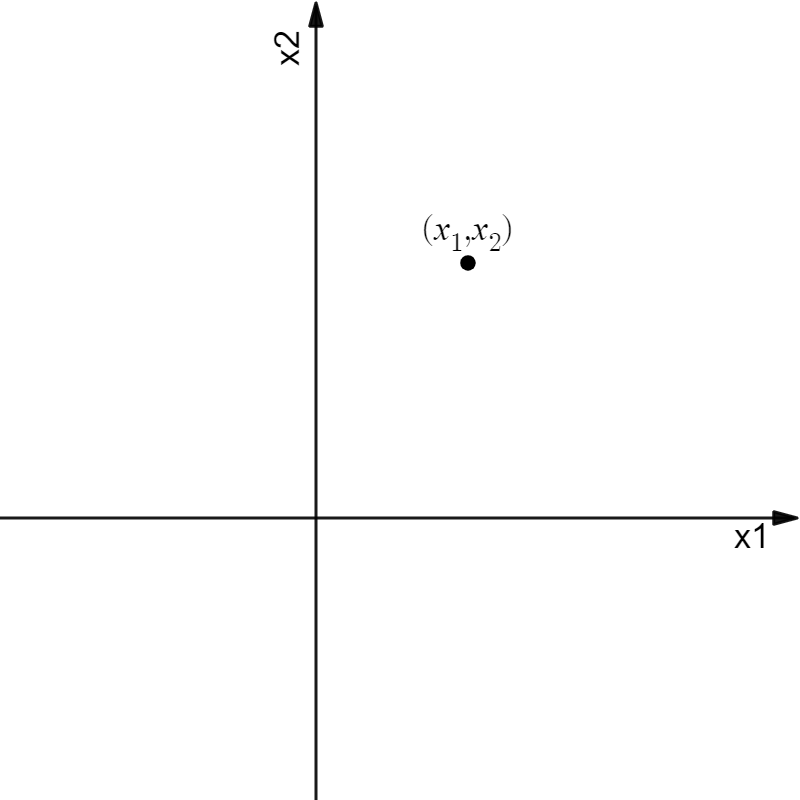
\includegraphics[width=0.5\linewidth]{images/vg0} 

}

\caption{A point in the plane}\label{fig:ptinr2}
\end{figure}

It's also helpful to think of \(\mathbb{R}^2\) as a collection of vectors. If we place a vector with its tail at the origin, its tip is at a point \((x_1,x_2)\). We name the vector by this point. This picture represents the (column) vector
\(\mathbf{v}=\begin{bmatrix}x_1\\x_2 \end{bmatrix}\). (Fig. \ref{fig:vecinr2})

\begin{figure}

{\centering 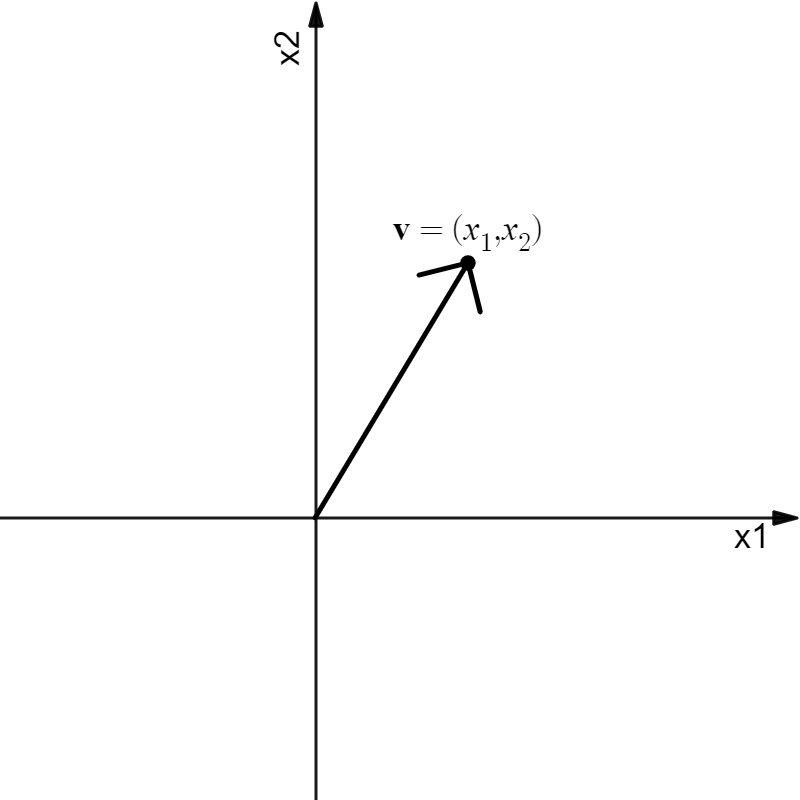
\includegraphics[width=0.5\linewidth]{images/vg1} 

}

\caption{A vector in $\mathbb{R}^2$}\label{fig:vecinr2}
\end{figure}

\subsection*{Vector addition and scalar multiplication}\label{vector-addition-and-scalar-multiplication}
\addcontentsline{toc}{subsection}{Vector addition and scalar multiplication}

We know how to add vectors because we know how to add matrices. If \(\mathbf{u}=\begin{bmatrix}u_1\\u_2\end{bmatrix}\) and \(\mathbf{v}=\begin{bmatrix}v_1\\v_2\end{bmatrix}\), then

\[\mathbf{u}+\mathbf{v}=\begin{bmatrix}u_1+v_1\\u_2+v_2\end{bmatrix}.\]

We also know how to multiply a vector by a scalar:

\[r\mathbf{u}=\begin{bmatrix} ru_1\\ru_2\end{bmatrix}.\]

For example, if \(\mathbf{u}=\begin{bmatrix}3\\5\end{bmatrix}\) and \(\mathbf{v}=\begin{bmatrix}2\\-1\end{bmatrix}\), then

\[\mathbf{u}+\mathbf{v}=\begin{bmatrix}3+2\\5+(-1)\end{bmatrix}=\begin{bmatrix}5\\4\end{bmatrix}.\]

Also,

\[2\mathbf{u}=\begin{bmatrix}2\cdot 3\\2\cdot 5\end{bmatrix}=\begin{bmatrix}6\\10\end{bmatrix},\]

while

\[-2\mathbf{u}=\begin{bmatrix}-2\cdot 3\\-2\cdot 5\end{bmatrix}=\begin{bmatrix}-6\\-10\end{bmatrix}.\]

Vector addition and scalar multiplication have nice geometric interpretations (Figures \ref{fig:vecadd},\ref{fig:scmult}).

\begin{figure}

{\centering 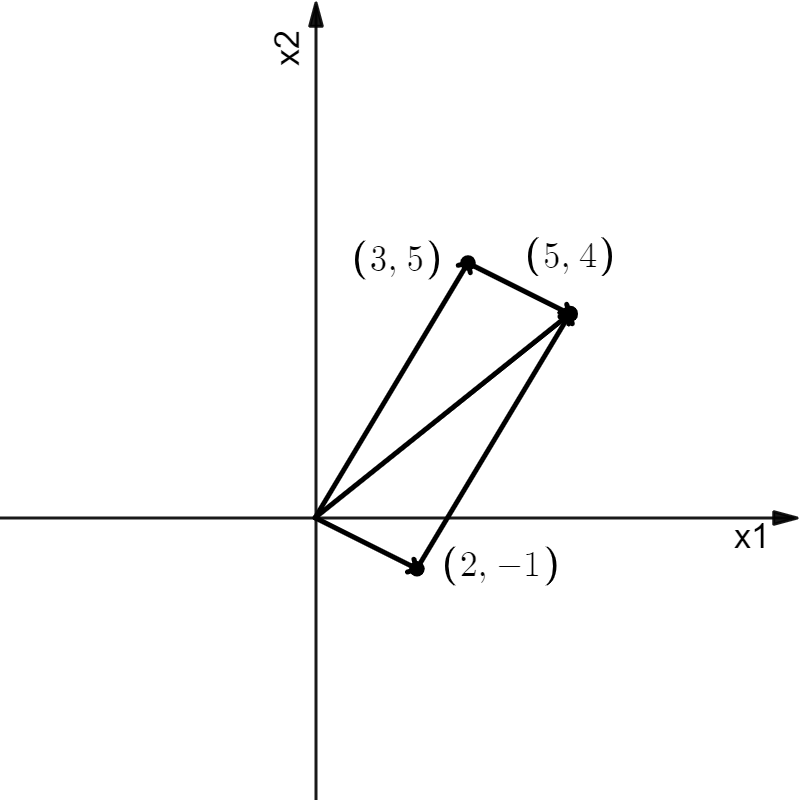
\includegraphics[width=0.5\linewidth]{images/vg2} 

}

\caption{Vector Addition}\label{fig:vecadd}
\end{figure}

\begin{figure}

{\centering 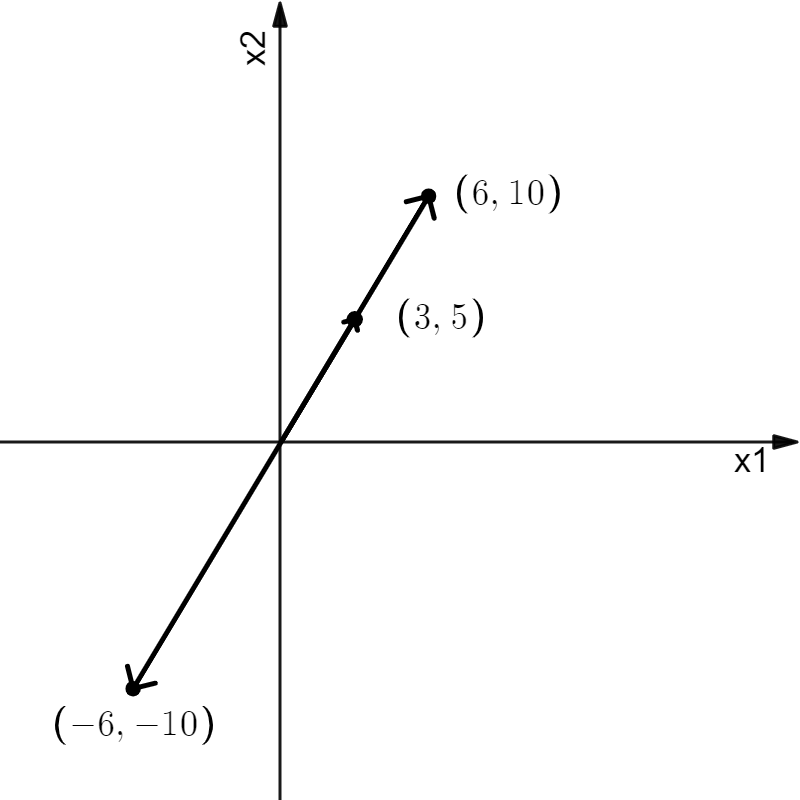
\includegraphics[width=0.5\linewidth]{images/vg3} 

}

\caption{Scalar Multiplication}\label{fig:scmult}
\end{figure}

We can't forget the special vector

\[\mathbf{0}=\begin{bmatrix}0\\0\end{bmatrix}.\]

Unlike the others, the zero vector has 0 magnitude and has no well-defined direction.

Speaking of magnitude, the \emph{magnitude} of a vector \(\mathbf{x}\), denoted \(|\mathbf{x}|\) (or frequently \(\Vert \mathbf{x}\Vert\)) is the distance from its tail to its tip. Using the Pythagorean theorem, if

\[\mathbf{x}=\begin{bmatrix}x_1\\x_2\end{bmatrix},\]

then

\[|\mathbf{x}|=\sqrt{x_1^2+x_2^2}.\]

For instance, if \(\mathbf{x}=\begin{bmatrix}2\\3\end{bmatrix}\), then \(|\mathbf{x}|=\sqrt{2^2+3^2}=\sqrt{13}\approx 3.6\).

With vector addition and scalar multiplication defined as above, we see that the following properties hold:

\begin{enumerate}
\def\labelenumi{\arabic{enumi}.}
\item
  If \(\mathbf{u}\) and \(\mathbf{v}\) are vectors in \(\mathbb{R}^2\), then \(\mathbf{u}+\mathbf{v}\) is also a vector in \(\mathbb{R}^2\). This property is called \emph{closure under addition}\index{Closure!under addition}.
\item
  If \(\mathbf{u}\) is a vector in \(\mathbb{R}^2\) and \(r\) is any real number, then \(r\mathbf{u}\) is also in \(\mathbb{R}^2\). This property is called \emph{closure under scalar multiplication}\index{Closure!under scalar multiplication}.
\end{enumerate}

Sets of things that satisfy these properties (and some others that we won't get into) are called \emph{vector spaces}\index{Vector space}.

\subsection*{Linear dependence and independence}\label{linear-dependence-and-independence}
\addcontentsline{toc}{subsection}{Linear dependence and independence}

Two vectors in \(\mathbb{R}^2\) are \emph{linearly dependent} if one is a constant multiple of the other. Otherwise, they are \emph{linearly independent}. For example,

\begin{enumerate}
\def\labelenumi{\arabic{enumi}.}
\item
  \(\mathbf{u}=\begin{bmatrix}2\\-3\end{bmatrix}\) and \(\mathbf{v}=\begin{bmatrix}-6\\9\end{bmatrix}\) are linearly dependent, since \(\mathbf{v}=-3\mathbf{u}\).
\item
  \(\mathbf{u}=\begin{bmatrix}2\\-3\end{bmatrix}\) and \(\mathbf{v}=\begin{bmatrix}6\\9\end{bmatrix}\) are linearly independent, since \(v_1=3u_1\), but \(v_2=-3u_2\).
\item
  The zero vector \(\mathbf{0}\) is linearly dependent with every vector since \(0\mathbf{u}=\mathbf{0}\).
\end{enumerate}

Here's an alternative definition of linear dependence that we will be able to extend to larger collections of vectors.

\begin{defbox}

\begin{definition}
\protect\hypertarget{def:linind}{}\label{def:linind}Two vectors \(\mathbf{u}\) and \(\mathbf{v}\) are \textbf{linearly dependent}\index{Linear dependence} if there exist scalars \(a\) and \(b\), \emph{not both zero}, such that

\[a\mathbf{u}+b\mathbf{v}=\mathbf{0}.\]

If \(\mathbf{u}\) and \(\mathbf{v}\) are not linearly dependent, then they are \textbf{linearly independent}\index{Linear independence}.
\end{definition}

\end{defbox}

For example, \(\mathbf{u}=\begin{bmatrix}2\\-3\end{bmatrix}\) and \(\mathbf{v}=\begin{bmatrix}-6\\9\end{bmatrix}\) are linearly dependent, since \(3\mathbf{u}+1\mathbf{v}=\mathbf{0}.\)

\subsection*{Linear Combinations}\label{linear-combinations}
\addcontentsline{toc}{subsection}{Linear Combinations}

Any sum of the form

\[a\mathbf{u}+b\mathbf{v}\]

is called a \emph{linear combination}\index{Linear combination} of \(\mathbf{u}\) and \(\mathbf{v}\). An alternative way of stating Definition \ref{def:linind} is that \emph{two vectors are linearly dependent if there is a nontrivial linear combination that results in the zero vector}. (\emph{Trivial} in this context means that all coefficients are 0.)

\subsection*{\texorpdfstring{\(\mathbb{R}^3\) and \(\mathbb{R}^n\)}{\textbackslash mathbb\{R\}\^{}3 and \textbackslash mathbb\{R\}\^{}n}}\label{mathbbr3-and-mathbbrn}
\addcontentsline{toc}{subsection}{\(\mathbb{R}^3\) and \(\mathbb{R}^n\)}

We can think of \(\mathbb{R}^3\) as a vector space, as well.

\[\mathbb{R}^3=\left\{\mathbf{x}=\begin{bmatrix}x_1\\x_2\\x_3\end{bmatrix}:x_1,x_2,x_3\in\mathbb{R}\right\}.\]

And, while we can't easily visualize higher dimensional vectors,
we can define \(\mathbb{R}^n\) for any positive integer \(n\) as a vector space:

\[\mathbb{R}^n=\left\{\mathbf{x}=\begin{bmatrix}x_1\\x_2\\ \vdots \\x_n\end{bmatrix}: x_1,x_2,\dots, x_n\in\mathbb{R}\right\}.\]

(Note: you can write these vectors horizontally: \((x_1,x_2,\dots,x_n)\) if necessary, to save space.)

The properties for vectors in \(\mathbb{R}^2\) have analogous properties in \(\mathbb{R}^n\). The magnitude of a vector is defined this way: if

\[\mathbf{x}=\begin{bmatrix}x_1\\x_2\\ \vdots \\x_n\end{bmatrix},\]

then

\[|\mathbf{x}|=\sqrt{x_1^2+x_2^2+\cdots+x_n^2}.\]

\section{Subspaces}\label{subspaces}

For what we will be doing in the future, \emph{subspaces} will be very important to us. Here's the definition.

\begin{defbox}

\begin{definition}
\protect\hypertarget{def:SubspaceDef}{}\label{def:SubspaceDef}Let \(W\) be a nonempty subset of a vector space \(V\). Then \(W\) is a \emph{subspace}\index{Subspace} of \(V\) if

\begin{enumerate}
\def\labelenumi{\arabic{enumi}.}
\item
  For all vectors \(\mathbf{w}_1\) and \(\mathbf{w}_2\) in \(W\), \(\mathbf{w}_1+\mathbf{w}_2\) is also in \(W\) (i.e.~\(W\) is closed under addition), and
\item
  For vectors \(\mathbf{w}\) in \(W\) and all scalars \(r\), \(r\mathbf{w}\) is also in \(W\) (i.e.~\(W\) is closed under scalar multiplication).
\end{enumerate}

These two can be combined into a single condition: a subset of a vector space is a subspace if all linear combinations of vectors from the subset are also in the subset.
\end{definition}

\end{defbox}

Essentially, a subspace is a subset of vector space that is itself a vector space.

\begin{examplebox}

\begin{example}
Let \(W\) be the set of all vectors in \(\mathbb{R}^3\) of the form

\[\mathbf{w}=\begin{bmatrix}w_1\\w_2\\w_3\end{bmatrix}\]

such that \(w_1+w_2+w_3=0\).

For instance, \(\mathbf{w}=\begin{bmatrix} 1\\2\\-3\end{bmatrix}\) is in \(W\), since \(1+2+(-3)=0\), but \(\mathbf{v}=\begin{bmatrix} 1\\2\\-4\end{bmatrix}\) is not in \(W\), since \(1+2+(-4)=-1\neq 0\). Is \(W\) a subspace of \(\mathbb{R}^3\)? We need to check closure under addition and closure under scalar multiplication.

\textbf{Closure under addition}: let \(\mathbf{w}=(w_1,w_2,w_3)\) and let \(\mathbf{v}=(v_1,v_2,v_3)\) be any two vectors in \(W\). (This means that \(w_1+w_2+w_3=0\) and \(v_1+v_2+v_3=0\).) Then \(\mathbf{w}+\mathbf{v}=(w_1+v_1,w_2+v_2,w_3+v_3)\).

We need to show that \(\mathbf{w}+\mathbf{v}\) is in \(W\), which means showing that the sum of the components of \(\mathbf{w}+\mathbf{v}\) is 0. We have

\begin{align*}
    (w_1+v_1)+(w_2+v_2)+(w_3+v_3)&=(w_1+w_2+w_3)+(v_1+v_2+v_3)\\
    &=0+0 \text{ since $\mathbf{w}$ and $\mathbf{v}$ are in $W$}\\
    &=0.\checkmark
\end{align*}

The sum of two vectors in \(W\) is also in \(W\).

\textbf{Closure under scalar multiplication}: Let \(\mathbf{w}=(w_1,w_2,w_3)\) be a vector in \(W\), and let \(r\) be any real number. Then \(r\mathbf{w}=(rw_1,rw_2,rw_3)\), and

\[rw_1+rw_2+rw_3=r(w_1+w_2+w_3)=r\cdot 0=0.\checkmark\]

Since \(W\) is closed under addition and scalar multiplication, it is a subspace of \(\mathbb{R}^3\).
\end{example}

\end{examplebox}

\begin{examplebox}

\begin{example}
Let \(W\) be the set of all vectors in \(\mathbb{R}^2\) of the form
\(\mathbf{w}=(w_1,1)\). (All vectors with a second component of 1.)
Is this \(W\) a subspace?

Nope. If \(\mathbf{w}=(w_1,1)\), then \(2\mathbf{w}=(2w_1,2)\), which is not in \(W\). Since \(W\) is not closed under scalar multiplication, it is not a subspace of \(\mathbb{R}^2\). It's also easy to show that \(W\) is not closed under addition.
\end{example}

\end{examplebox}

Suppose that \(W\) is a subspace, and let \(\mathbf{w}\) be any vector in \(W\). Then the scalar product \(0\mathbf{w}=\mathbf{0}\) must also be in \(W\). In other words, any subspace (and any vector space, for that matter) must contain a zero vector. If a subset of a vector space does not contain the zero vector, it cannot be a subspace.
In our last example, \(W\) did not contain the zero vector, since \(\mathbf{0}=(0,0)\) is not of the form \((w_1,1)\). We could have immediately determined that \(W\) was not a subspace.

Let's state this fact about the zero vector as a theorem.

\begin{theorembox}

\begin{theorem}
\protect\hypertarget{thm:zerovector}{}\label{thm:zerovector}Let \(W\) be a subspace of a vector space \(V\). Then \(\mathbf{0}\in W.\)
\end{theorem}

\end{theorembox}

Here is one last example to close out the section.

\begin{examplebox}

\begin{example}
\protect\hypertarget{exm:Nullspace}{}\label{exm:Nullspace}Let \(\mathbf{A}\) be an \(m\times n\) matrix, and let \(W\) be the set of all vectors \(\mathbf{x}\) in \(\mathbb{R}^n\) such that \(\mathbf{A}\mathbf{x}=\mathbf{0}\). Is \(W\) a subspace of \(\mathbb{R}^n\)?

\textbf{Closure under addition}: let \(\mathbf{x}\) and \(\mathbf{y}\) be two vectors in \(W\). Then

\begin{align*}
\mathbf{A}\left(\mathbf{x}+\mathbf{y}\right)&=\mathbf{A}\mathbf{x}+\mathbf{A}\mathbf{y}\\
&=\mathbf{0}+\mathbf{0}=\mathbf{0}.\checkmark
\end{align*}

\textbf{Closure under scalar multiplication}: if \(\mathbf{x}\) is in \(W\) and \(r\) is any real number, then

\[\mathbf{A}(r\mathbf{x})=r(\mathbf{A}\mathbf{x})=r\mathbf{0}=\mathbf{0}.\checkmark\]

So \(W\) is a subspace of \(\mathbb{R}^n\), and an important one, called the \emph{nullspace}\index{Nullspace} of \(\mathbf{A}\). We'll see more of it in the future.
\end{example}

\end{examplebox}

\section{Linear Dependence and Independence}\label{linear-dependence-and-independence-1}

In Section \ref{artoo}, we talked about a linear combination of two vectors. Let's generalize the notion.

\begin{defbox}

\begin{definition}
\protect\hypertarget{def:LinComb}{}\label{def:LinComb}Let \(\{\mathbf{v}_1,\mathbf{v}_2,\dots,\mathbf{v}_r\}\)
be a collection of vectors in a vector space \(V\). A \textbf{linear combination}\index{Linear combination} of \(\{\mathbf{v}_1,\mathbf{v}_2,\dots,\mathbf{v}_r\}\) is a vector

\[\mathbf{v}=c_1\mathbf{v}_1+c_2\mathbf{v}_2+\cdots+c_r\mathbf{v}_r,\]

where \(c_1,c_2,\dots,c_r\) are real numbers.
\end{definition}

\end{defbox}

\begin{examplebox}

\begin{example}
Let

\[\mathbf{v}_1=\begin{bmatrix} 1\\2\\1\end{bmatrix},\mathbf{v}_2=\begin{bmatrix} 2\\3\\-1\end{bmatrix}, \text{ and }\mathbf{v}_3=\begin{bmatrix}4\\1\\2\end{bmatrix}.\]

Then \(\mathbf{v}=2\mathbf{v}_1+\mathbf{v}_2-3\mathbf{v}_3\) is
\begin{align*}\mathbf{v}=2\begin{bmatrix} 1\\2\\1\end{bmatrix}+1\begin{bmatrix} 2\\3\\-1\end{bmatrix}-3\begin{bmatrix}4\\1\\2\end{bmatrix}&=\begin{bmatrix}2\cdot 1+1\cdot 2-3\cdot 4\\2\cdot 2+1\cdot 3-3\cdot 1\\2\cdot 1+1\cdot(-1)-3\cdot 2\end{bmatrix}\\
&=\begin{bmatrix}-8\\4\\-5\end{bmatrix}.
\end{align*}
\end{example}

\end{examplebox}

This type of calculation might seem familiar. Consider the matrix-vector product \(\mathbf{A}\mathbf{x}\):

\[\mathbf{A}\mathbf{x}=\begin{bmatrix}1 & 2 & 4\\2 & 3 & 1\\1 & -1 & 2\end{bmatrix}\begin{bmatrix}2\\1\\-3\end{bmatrix}=\begin{bmatrix}-8\\4\\-5\end{bmatrix}.\]

Note that the columns of \(\mathbf{A}\) are the vectors \(\mathbf{v}_1,\mathbf{v}_2,\) and \(\mathbf{v}_3\) from the last example, while the entries in \(\mathbf{x}\) are the coefficients in the linear combination from the example. When you multiply a vector by a matrix, you're really just taking a linear combination of the columns of the matrix! This is an important and useful idea.

Here it is in more general form:

\[\begin{bmatrix}a_{11} & a_{12} &\cdots & a_{1n}\\
a_{21} & a_{22} & \cdots & a_{2n}\\
\vdots & \vdots & \ddots & \vdots \\
a_{m1} & a_{m2} & \cdots & a_{mn}\end{bmatrix}
\begin{bmatrix} c_1\\c_2\\ \vdots\\c_n\end{bmatrix}=
c_1\mathbf{a}_1+c_2\mathbf{a}_2+\cdots+c_n\mathbf{a}_n,\]
where \(\mathbf{a}_i\) is the \(i\)th column vector.

(Here is some useful notation: the matrix with columns \(\mathbf{a}_1,\mathbf{a}_2,\dots,\mathbf{a}_n\) is often written \(\begin{bmatrix}\mathbf{a}_1&\mathbf{a}_2&\cdots&\mathbf{a}_n\end{bmatrix}\). Note the bold typeface indicating vectors.)

One important result of this is that the equation \(\mathbf{A}\mathbf{x}=\mathbf{b}\) has a solution if and only if \(\mathbf{b}\) can be written as a linear combination of the columns of \(\mathbf{A}\).

\begin{examplebox}

\begin{example}
Can \(\mathbf{b}=\begin{bmatrix}2\\5\end{bmatrix}\) be written as a linear combination of \(\mathbf{a}_1=\begin{bmatrix}1\\2\end{bmatrix}\) and \(\mathbf{a}_2=\begin{bmatrix}4\\7\end{bmatrix}\)? This is equivalent to solving \(\begin{bmatrix}\mathbf{a}_1 & \mathbf{a}_2\end{bmatrix}\begin{bmatrix}c_1\\c_2\end{bmatrix}=\mathbf{b}\)

To solve this, we'll create the matrix \(\mathbf{A}\) with \(\mathbf{a}_1\) and \(\mathbf{a}_2\) as its columns, augment it with \(\mathbf{b}\), and reduce:\footnote{Of course, we could also use inverses or technology.}

\[\left[ \begin{array}{ll|l} 1 & 4 & 2\\2 & 7 & 5\end{array}\right]\leadsto \left[ \begin{array}{ll|l} 1 & 0 & 6\\0 & 1 & -1\end{array}\right]\]

The answer is yes, with the combination \(\mathbf{b}=6\mathbf{a}_1-\mathbf{a}_2\). To verify this, we have

\[6\mathbf{a}_1-\mathbf{a}_2=6\begin{bmatrix}1\\2\end{bmatrix}-\begin{bmatrix}4\\7\end{bmatrix}=\begin{bmatrix}6\cdot 1-1\cdot 4\\6\cdot 2-1\cdot 7\end{bmatrix}=\begin{bmatrix}2\\5\end{bmatrix}=\mathbf{b}.\]
\end{example}

\end{examplebox}

The \emph{span} of a set of vectors is an important concept.

\begin{defbox}

\begin{definition}
\protect\hypertarget{def:span}{}\label{def:span}Let \(\{\mathbf{v}_1,\mathbf{v}_2,\dots,\mathbf{v}_r\}\) be a set of vectors in a vector space \(V\). The \textbf{span}\index{Span} of the set,
\(\text{span}(\mathbf{v}_1,\mathbf{v}_2,\dots,\mathbf{v}_r)\),
is the set of all possible linear combinations of the vectors.
\end{definition}

\end{defbox}

The following theorem is important and easy to prove.

\begin{theorembox}

\begin{theorem}
Let \(\{\mathbf{v}_1,\mathbf{v}_2,\dots,\mathbf{v}_r\}\) be a set of vectors in a vector space \(V\). Then \(W=\textrm{span}(\mathbf{v}_1,\mathbf{v}_2,\dots,\mathbf{v}_r)\) is a subspace of \(V\).
\end{theorem}

\end{theorembox}

\begin{proof}
Let \(\mathbf{u}\) and \(\mathbf{w}\) be in \(W\). There exist constants \(a_1,\dots,a_r\) and \(b_1,\dots,b_r\) such that \(\mathbf{u}=a_1\mathbf{v}_1+\cdots + a_r\mathbf{v}_r\) and \(\mathbf{w}=b_1\mathbf{v}_1+\cdots + b_r\mathbf{v}_r.\) Then \(\mathbf{u}+\mathbf{w}=(a_1+b_1)\mathbf{v}_1+\cdots+(a_r+b_r)\mathbf{v}_r\), which is another linear combination of \(\mathbf{v}_1\dots,\mathbf{v}_r,\) so it is in \(W\).

Similarly, for any scalar \(c,c\mathbf{u}=ca_1\mathbf{v}_1+\cdots+ca_r\mathbf{v}_r.\) Since \(W\) is closed under addition and scalar multiplication, it is a subspace of \(V\).
\end{proof}

\subsection*{Linear dependence revisited}\label{linear-dependence-revisited}
\addcontentsline{toc}{subsection}{Linear dependence revisited}

Let's now generalize the definitions of linear dependence and independence.

\begin{defbox}

\begin{definition}
Let \(\mathbf{v}_1,\mathbf{v}_2,\dots,\mathbf{v}_r\) be vectors in a vector space \(V\). The vectors are \textbf{linearly dependent}\index{Linear dependence} if there exist constants \(c_1,c_2,\dots,c_r\), not all zero, such that

\[c_1\mathbf{v}_1+c_2\mathbf{v}_2+\cdots+c_r\mathbf{v}_r=\mathbf{0}.\]

If the set is not linearly dependent, then it is \textbf{linearly independent}\index{Linear independence}.
\end{definition}

\end{defbox}

Note that any collection that includes the zero vector will be linearly dependent. Why? Suppose \(\{\mathbf{v}_1,\dots \mathbf{v}_r, \mathbf{0}\}\) is the set in question. Then

\[0\mathbf{v}_1+\cdots+0\mathbf{v}_r+1\cdot \mathbf{0}=\mathbf{0},\]

a nontrivial linear combination yielding the zero vector.

Also note that if a collection of vectors is linearly dependent, than at least one can be written as a linear combination of the others.

\begin{examplebox}

\begin{example}
\protect\hypertarget{exm:ldepex1}{}\label{exm:ldepex1}Let \(\mathbf{v}_1=(1,2,-1),\mathbf{v}_2=(2,-1,4)\), and \(\mathbf{v}_3=(3,-4,9)\). Are these vectors dependent or independent?

To answer this question, we can put the vectors as columns in a matrix \(\mathbf{A}\) and see if the equation \(\mathbf{A}\mathbf{c}=\mathbf{0}\) has a nontrivial solution. (Again, remember that \(\mathbf{A}\mathbf{c}\) is a linear combination of the columns of \(\mathbf{A}\).)

\[\left[\begin{array}{rrr|r}1 & 2 & 3 & 0\\2 & -1 & -4 & 0\\-1 & 4 & 9 & 0\end{array}\right]\leadsto
\left[\begin{array}{rrr|r} 1 & 0 & -1 & 0\\0 & 1 & 2 & 0\\0 & 0 & 0 & 0\end{array}\right]\]

Since the reduced row echelon form of the coefficient matrix has a free variable, there will actually be infinitely many solutions. If we let \(c_3=t\), then \(c_1-t=0\) or \(c_1=t\), and \(c_2+2t=0\) or \(c_2=-2t\). In particular, if \(t=1\), then \(c_1=1,c_2=-2,\) and \(c_3=1\) will work. Let's check.

\[1\begin{bmatrix}1\\2\\-1\end{bmatrix}+-2\begin{bmatrix}2\\-1\\4\end{bmatrix}+1\begin{bmatrix}3\\-4\\9\end{bmatrix}=\begin{bmatrix}0\\0\\0\end{bmatrix}\checkmark.\]

Since we've found a nontrivial linear combination adding up to the zero vector, the three vectors are linearly dependent.
\end{example}

\end{examplebox}

\begin{examplebox}

\begin{example}
\protect\hypertarget{exm:lindex2}{}\label{exm:lindex2}Let \(\mathbf{v}_1=(1,2,-1),\mathbf{v}_2=(2,3,4)\), and \(\mathbf{v}_3=(3,5,4)\). Are these vectors linearly dependent or independent?

\[\left[\begin{array}{rrr|r}1 & 2 & 3 & 0\\2 & 3 & 5 & 0\\-1 & 4 & 4 & 0\end{array}\right]\leadsto \left[\begin{array}{rrr|r}1 & 0 & 0 & 0\\0 & 1 & 0 & 0\\0 & 0 & 1 & 0\end{array}\right]\]

In this case, the only solution is the trivial one: \(c_1=c_2=c_3=0\). The vectors are linearly independent.
\end{example}

\end{examplebox}

In both of these examples, we were dealing with three vectors in \(\mathbb{R}^3\). The process will still work with any number of vectors in any dimension of vector space, but there is a nice connection when the number of vectors is equal to the dimension of the vector space. First, a quick definition.

\begin{defbox}

\begin{definition}
Two \(m\times n\) matrices are \textbf{row equivalent}\index{Row equivalent} if one can be transformed into the other via a sequence of elementary row operations.
\end{definition}

\end{defbox}

Note that since row operations are reversible, if you can transform \(\mathbf{A}\) to \(\mathbf{B}\), you can transform \(\mathbf{B}\) to \(\mathbf{A}\) by reversing the steps.

In Example \ref{exm:ldepex1}, when we reduced the matrix, we had a row of zeros at the bottom. In that case, the vectors were dependent. In Example \ref{exm:lindex2}, the coefficient matrix reduced to the identity matrix. Here's a theorem.

\begin{theorembox}

\begin{theorem}
Let \(\left\{\mathbf{v}_1,\mathbf{v}_2,\dots\mathbf{v}_n\right\}\) be a collection of \(n\) vectors in \(\mathbb{R}^n\). Let \(\mathbf{A}\) be the matrix whose columns are \(\mathbf{v}_1,\mathbf{v}_2,\dots\mathbf{v}_n\). Then \(\left\{\mathbf{v}_1,\mathbf{v}_2,\dots\mathbf{v}_n\right\}\) are linearly \emph{independent} if and only if \(\mathbf{A}\) is row equivalent to the identity matrix.

Equivalently, \(\left\{\mathbf{v}_1,\mathbf{v}_2,\dots\mathbf{v}_n\right\}\) are linearly \emph{dependent} if and only if \(\det\mathbf{A}=0\) if and only if \(\mathbf{A}\) is invertible.
\end{theorem}

\end{theorembox}

The key thing here is that the number of vectors matches the dimension. There are only zeros to the right of the augmentation bar, and when you perform any row operations, there will still be only zeros there. If the coefficient part reduces to the identity matrix, you will have only the trivial solution. Otherwise, there will be a free variable and infinitely many solutions.

Note that if \(\left\{\mathbf{v}_1,\mathbf{v}_2,\dots,\mathbf{v}_n\right\}\) is a linearly independent collection of vectors in \(\mathbb{R}^n\) and \(\mathbf{v}\) is any vector in \(\mathbb{R}^n\), then we can write \(\mathbf{v}\) as a linear combination of \(\mathbf{v}_1,\mathbf{v}_2,\dots,\mathbf{v}_n\). Why? Since

\[\mathbf{A}=\begin{bmatrix} \mathbf{v}_1 & \mathbf{v}_2 & \cdots & \mathbf{v}_n\end{bmatrix}\]

is invertible,

\[\mathbf{A}\mathbf{x}=\mathbf{v}\]

has a solution, and the entries in \(\mathbf{x}\) give us the coefficients in the linear combination. We say that a linearly independent collection of \(n\) vectors in \(\mathbb{R}^n\) \emph{spans} \(\mathbb{R}^n\).

What happens when you have more than \(n\) vectors in \(\mathbb{R}^n\)? Here's a quick example with 3 vectors in \(\mathbb{R}^2\). (We'll put them in the columns.)

\[\left[\begin{array}{rrr|r} 1 & 2 & 3 & 0\\ 2 & 4 & 1 & 0\end{array}\right]\leadsto \left[\begin{array}{rrr|r}1 & 2 & 0 & 0\\0 & 0 & 1 & 0\end{array}\right]\]

Since there's a free variable, \(c_2\) (the second coefficient) in this case, there will be infinitely many solutions. Whenever there are more columns than rows in the coefficient matrix there will be a free variable.
If the number of vectors is greater than the dimension of the vector space, the set will always be linearly dependent. Let's make that a theorem.

\begin{theorembox}

\begin{theorem}
Let \(\left\{\mathbf{v}_1,\dots,\mathbf{v}_n\right\}\) be a set of \(n\) vectors in \(\mathbb{R}^m\), with \(n>m\). Then \(\left\{\mathbf{v}_1,\dots,\mathbf{v}_n\right\}\) is a linearly dependent set.
\end{theorem}

\end{theorembox}

\section{Basis and Dimension}\label{basis-and-dimension}

Let \(\mathbf{u}=\begin{bmatrix}u_1\\u_2\end{bmatrix}\) be any vector in \(\mathbb{R}^2\), and let \(\mathbf{e}_1=\begin{bmatrix}1\\0\end{bmatrix}\) and \(\mathbf{e}_2=\begin{bmatrix}0\\1\end{bmatrix}\).

(You may have seen \(\mathbf{e}_1\) and \(\mathbf{e}_2\) called \(\mathbf{i}\) and \(\mathbf{j},\) respectively, but we will be generalizing them soon, and we run out of letters quickly.)

The key observation is that \(\mathbf{u}\) can be written as a linear combination of \(\mathbf{e}_1\) and \(\mathbf{e}_2\) this way:

\[\mathbf{u}=\begin{bmatrix}u_1\\u_2\end{bmatrix}=\begin{bmatrix}u_1\\0\end{bmatrix}+\begin{bmatrix}0\\u_2\end{bmatrix}=u_1\begin{bmatrix}1\\0\end{bmatrix}+u_2\begin{bmatrix}0\\1\end{bmatrix}=u_1\mathbf{e}_1+u_2\mathbf{e}_2.\]

The geometry of this linear combination looks like this (Fig. \ref{fig:stdbasispic}).

\begin{figure}

{\centering 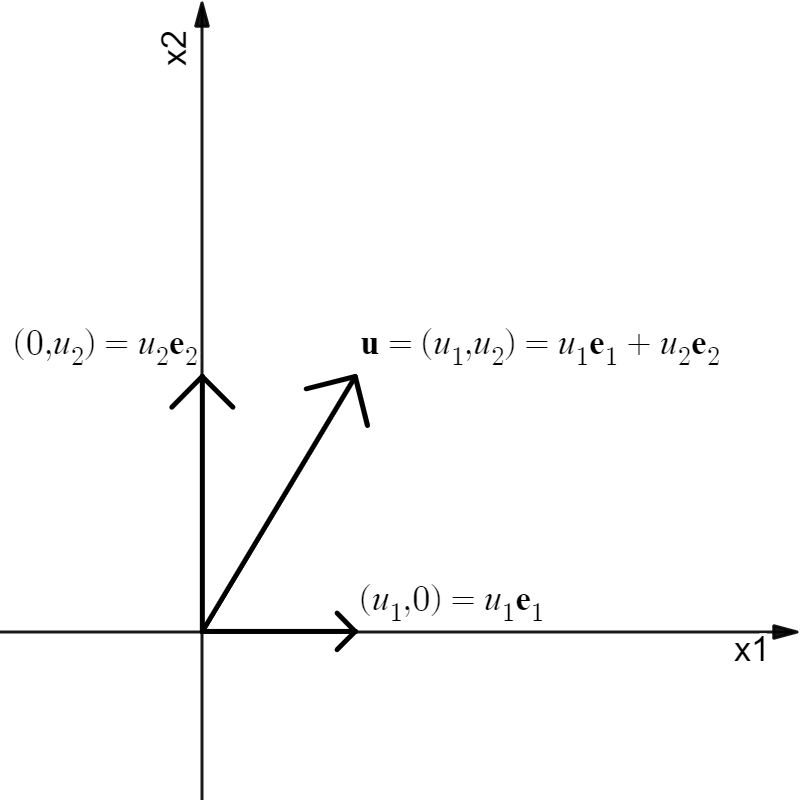
\includegraphics[width=0.5\linewidth]{images/sbv} 

}

\caption{Writing a vector in terms of $\mathbf{e}_1$ and $\mathbf{e}_2$}\label{fig:stdbasispic}
\end{figure}

The vectors \(\mathbf{e}_1\) and \(\mathbf{e}_2\) have the following properties:

\begin{enumerate}
\def\labelenumi{\arabic{enumi}.}
\item
  \(\mathbf{e}_1\) and \(\mathbf{e}_2\) are linearly independent.
\item
  Any vector in \(\mathbb{R}^2\) can be written as a linear combination of \(\mathbf{e}_1\) and \(\mathbf{e}_2\). That is, they span \(\mathbb{R}^2\).
\end{enumerate}

These properties define a \emph{basis} for a vector space.

\begin{defbox}

\begin{definition}
A \textbf{basis}\index{Basis} for a vector space \(V\) is a collection of linearly independent vectors \(\{\mathbf{v}_1,\mathbf{v}_2,\dots,\mathbf{v}_r\}\)
whose span is all of \(V\).
\end{definition}

\end{defbox}

While \(\{\mathbf{e}_1,\mathbf{e}_2\}\) is a basis for \(\mathbb{R}^2\), it is not the only one. In fact, as we learned in the last section, any linearly independent pair of vectors in \(\mathbb{R}^2\) will span \(\mathbb{R}^2\). We do, however, have the following fact about bases which we won't prove.

\begin{theorembox}

\begin{theorem}
Let \(\{\mathbf{u}_1,\mathbf{u}_2,\dots,\mathbf{u}_r\}\) and \(\{\mathbf{v}_1,\mathbf{v}_2\dots,\mathbf{v}_s\}\) be two bases for a vector space \(V\). Then \(r=s\). This common value is the \textbf{dimension}\index{Dimension!of a vector space} of \(V\).
\end{theorem}

\end{theorembox}

Note: there are such things as infinite dimensional vector spaces, but we won't be dealing with them in this book.

\subsection*{\texorpdfstring{The standard basis for \(\mathbb{R}^n\)}{The standard basis for \textbackslash mathbb\{R\}\^{}n}}\label{the-standard-basis-for-mathbbrn}
\addcontentsline{toc}{subsection}{The standard basis for \(\mathbb{R}^n\)}

The \emph{standard basis}\index{Basis!standard} for \(\mathbb{R}^3\) is

\[\mathbf{e}_1=\begin{bmatrix} 1\\0\\0\end{bmatrix},\mathbf{e}_2=\begin{bmatrix}0\\1\\0\end{bmatrix},\mathbf{e}_3=\begin{bmatrix}0\\0\\1\end{bmatrix}.\]

(You might know them better as \(\mathbf{i},\) \(\mathbf{j},\) and \(\mathbf{k}.\))

The standard basis for \(\mathbb{R}^n\) is the set of vectors \(\{\mathbf{e}_i,i=1\dots n\}\), where \(\mathbf{e}_i\) is the \(n\)-dimensional vector with a 1 in the \(i\)th entry, and zeros everywhere else.

Remember that any collection of \(n\) linearly independent vectors in \(\mathbb{R}^n\) will span \(\mathbb{R}^n\) and, thus, form a basis for it.

\subsection*{The dimension of a subspace}\label{the-dimension-of-a-subspace}
\addcontentsline{toc}{subsection}{The dimension of a subspace}

Since a subspace of a finite dimensional vector space is a vector space in its own right, it will have its own dimension. If we can find a basis, we will know its dimension\index{Dimension!of a subspace}.

\subsection*{The dimension of the Nullspace}\label{the-dimension-of-the-nullspace}
\addcontentsline{toc}{subsection}{The dimension of the Nullspace}

We talked about the nullspace\index{Nullspace} of an \(m\times n\) matrix \(\mathbf{A}\) in Example \ref{exm:Nullspace} . It's the set of all vectors \(\mathbf{x}\) in \(\mathbb{R}^n\) such that \(\mathbf{A}\mathbf{x}=\mathbf{0}.\) Let's call it \(\text{Null}(\mathbf{A})\). If we can find a basis for \(\text{Null}(\mathbf{A})\), we can find its dimension as a subspace of \(\mathbb{R}^n\).

\begin{examplebox}

\begin{example}
Find a basis for \(\text{Null}(\mathbf{A})\), where

\[\mathbf{A}=\begin{bmatrix}5 & 2 & -15 & 8\\2 & 1 & -6 & 3\\-3 & -1 & 9 & -5\end{bmatrix}.\]

To solve \(\mathbf{A}\mathbf{x}=\mathbf{0}\), we augment \(\mathbf{A}\) with the zero vector and put in reduced row echelon form.

\[\left[\begin{array}{rrrr|r}5 & 2 & -15 & 8 & 0\\2 & 1 & -6 & 3& 0\\-3 & -1 & 9 & -5& 0\end{array}\right]\leadsto \left[\begin{array}{rrrr|r} 1 & 0 & -3 & 2 & 0\\0 & 1 & 0 & -1 & 0\\0 & 0 & 0 & 0 & 0\end{array}\right]\]

With the columns representing \(x_1,x_2,x_3,\) and \(x_4\), we have \(x_3\) and \(x_4\) as free variables. If we let \(s=x_3\) and \(t=x_4\), then \(x_1=3s-2t\) and \(x_2=t\).

We can write the solution to \(\mathbf{A}\mathbf{x}=\mathbf{0}\) in parametric form as

\[\begin{bmatrix}x_1\\x_2\\x_3\\x_4\end{bmatrix}=\begin{bmatrix}3s-2t\\t\\s\\t\end{bmatrix}=s\begin{bmatrix}3\\0\\1\\0\end{bmatrix}+t\begin{bmatrix}-2\\1\\0\\1\end{bmatrix}.\]

The vectors

\[\mathbf{v}_1=\begin{bmatrix}3\\0\\1\\0\end{bmatrix} \text{ and } \mathbf{v}_2=\begin{bmatrix}-2\\1\\0\\1\end{bmatrix}\]

form our basis for \(\text{Null}(\mathbf{A})\), which is a 2-dimensional subspace of \(\mathbb{R}^4\). Note that the dimension corresponds to the number of free variables in the reduced row echelon form of \(\mathbf{A}.\) This number is sometimes called the \emph{nullity}\index{Nullity} of \(\mathbf{A}.\) As a check, note that

\[\mathbf{A}\mathbf{v}_1=\begin{bmatrix}5 & 2 & -15 & 8\\2 & 1 & -6 & 3\\-3 & -1 & 9 & -5\end{bmatrix}\begin{bmatrix}3\\0\\1\\0\end{bmatrix}=3\begin{bmatrix}5\\2\\-3\end{bmatrix}+\begin{bmatrix}-15\\-6\\9\end{bmatrix}=\begin{bmatrix}0\\0\\0\end{bmatrix}=\mathbf{0}.\]

This calculation shows that \(\mathbf{v}_1\) is in the nullspace of \(\mathbf{A}\). A similar calculation will show that \(\mathbf{v}_2\) is also in it.
\end{example}

\end{examplebox}

One last note: if \(\mathbf{A}\mathbf{x}=\mathbf{0}\) has only the trivial solution \(\mathbf{x}=\mathbf{0}\), then \(\text{Null}(\mathbf{A})\) is said to have dimension 0.

\subsection*{The column space of a matrix}\label{the-column-space-of-a-matrix}
\addcontentsline{toc}{subsection}{The column space of a matrix}

\begin{defbox}

\begin{definition}
Let \(\mathbf{A}=\begin{bmatrix}\mathbf{a}_1 & \mathbf{a}_2&\cdots & \mathbf{a}_n\end{bmatrix}\) be an \(m\times n\) matrix. (Recall that the columns of \(\mathbf{A},\) \(\{\mathbf{a}_1,\mathbf{a}_2,\dots,\mathbf{a}_n\}\) are vectors in \(\mathbb{R}^m\).)
The \textbf{column space}\index{Column space} of \(\mathbf{A},\) denoted \(\text{Col}(\mathbf{A})\), is the span of \(\{\mathbf{a}_1,\mathbf{a}_2,\dots,\mathbf{a}_n\}\).
Note that \(\text{Col}(\mathbf{A})\) is a subspace of \(\mathbb{R}^m\).
\end{definition}

\end{defbox}

Recall that the equation \(\mathbf{A}\mathbf{x}=\mathbf{b}\) has a solution if and only if \(\mathbf{b}\) is a linear combination of the columns of \(\mathbf{A},\) which means that \(\mathbf{b}\) has to be in the column space of \(\mathbf{A}.\)

\begin{theorembox}

\begin{theorem}
Let \(\mathbf{A}\) be an \(m\times n\) matrix, and let \(\mathbf{b}\) be a vector in \(\mathbb{R}^m\). Then the equation \(\mathbf{A}\mathbf{x}=\mathbf{b}\) has a solution if and only if \(\mathbf{b}\) is in the column space of \(\mathbf{A}.\)
\end{theorem}

\end{theorembox}

\begin{examplebox}

\begin{example}
\protect\hypertarget{exm:colspex}{}\label{exm:colspex}It turns out, that the process of finding a basis for the nullspace of \(\mathbf{A}\) will also give you the basis for the column space. The reasoning is a bit tricky, but the process is simple. Recall the last example we did, leaving off the augmented vector.

\[\mathbf{A}=\begin{bmatrix}5 & 2 & -15 & 8 \\2 & 1 & -6 & 3\\-3 & -1 & 9 & -5\end{bmatrix}\leadsto \begin{bmatrix} 1 & 0 & -3 & 2 \\0 & 1 & 0 & -1 \\0 & 0 & 0 & 0 \end{bmatrix}\]

The reduced row echelon form of \(\mathbf{A}\) has two pivot columns (columns with leading 1's): column 1 and column 2. The corresponding columns of \(\mathbf{A}\) will form a basis for \(\text{Col}(\mathbf{A})\). Our basis is

\[\left\{\left[\begin{array}{rrr}5\\2\\-3\end{array}\right],\left[\begin{array}{rrr} 2\\1\\-1\end{array}\right]\right\}.\]
\end{example}

\end{examplebox}

This is the procedure for identifying a basis for the column space of a matrix \(\mathbf{A}\).

\begin{enumerate}
\def\labelenumi{\arabic{enumi}.}
\item
  Put \(\mathbf{A}\) in to reduced row echelon form, call it \(\mathbf{R}.\) (Actually, just row echelon form is sufficient.)
\item
  Identify the pivot columns of \(\mathbf{R}.\) These are the columns with leading ones.
\item
  The columns of \(\mathbf{A}\) corresponding to the pivot columns of \(\mathbf{R}\) form a basis for \(\text{Col}(\mathbf{A}).\)
\end{enumerate}

Basically, elementary row operations preserve column dependencies, though they do not preserve the column space itself. The pivot columns of \(\mathbf{R}\) form a basis for its column space, so the corresponding columns of \(\mathbf{A}\) form a basis for its column space.

Now that we know how to find a basis for the column space of a matrix, we know what the dimension of the space is.

\begin{defbox}

\begin{definition}
Let \(\mathbf{A}\) be an \(m\times n\) matrix. The \textbf{column rank}\index{Rank!Column} of \(\mathbf{A}\) is the dimension of the column space of \(\mathbf{A}.\)
\end{definition}

\end{defbox}

In Example \ref{exm:colspex}, the column rank is 2, since the column space has two basis vectors.

Note that the column rank of a matrix is equal to the number of pivot columns. The nullity of a matrix is equal to the number of free variables, which is the number of columns that aren't pivot columns. When you add these two numbers together, you get the total number of columns in the matrix. This leads to the following result.

\begin{theorembox}

\begin{theorem}
Let \(\mathbf{A}\) be an \(m\times n\) matrix. Then

\[\text{dim}\, \text{Col}(\mathbf{A)}+\text{dim}\, \text{Null}(\mathbf{A})=n.\]
\end{theorem}

\end{theorembox}

For example, if \(\mathbf{A}\) is a \(3\times 5\) matrix with a nullity of 2, then the column rank is \(5-2=3\).

\subsection*{The row space}\label{the-row-space}
\addcontentsline{toc}{subsection}{The row space}

The \emph{row space}\index{Row space} of a matrix \(\mathbf{A}\), denoted \(\text{Row}(\mathbf{A}),\) is the span of the row vectors of \(\mathbf{A}.\) It turns out that we can find a basis for the row space at the same time we're finding a basis for the column space and the nullspace. Again, we row reduce.

\begin{theorembox}

\begin{theorem}
The nonzero rows of the row reduced coefficient matrix form a basis for the row space.
\end{theorem}

\end{theorembox}

Let's go back to our example.

\[\mathbf{A}=\begin{bmatrix}5 & 2 & -15 & 8 \\2 & 1 & -6 & 3\\-3 & -1 & 9 & -5\end{bmatrix}\leadsto \begin{bmatrix} 1 & 0 & -3 & 2 \\0 & 1 & 0 & -1 \\0 & 0 & 0 & 0 \end{bmatrix}\]

Our basis is

\[\left\{\begin{bmatrix}1 &0 & -3 & 2\end{bmatrix},\begin{bmatrix}0 & 1 & 0 & -1\end{bmatrix}\right\}.\]

This one is easier to explain. Elementary row operations at most produce vectors that are still in the row space.

\begin{enumerate}
\def\labelenumi{\arabic{enumi})}
\item
  Adding a multiple of one row to another: \(c\mathbf{r}_i+\mathbf{r}_j\) is in \(\text{Row}(\mathbf{A}).\)
\item
  Multiplying a row by a nonzero constant: \(c\mathbf{r}_i\) is in \(\text{Row}(\mathbf{A}).\)
\item
  Interchanging two rows just rearranges the vectors.
\end{enumerate}

This means that the rows of the reduced matrix, call it \(\mathbf{R},\) are in the span of the rows of \(\mathbf{A}.\)

Since row operations are reversible, the rows of \(\mathbf{A}\) are also linear combinations of the rows of \(\mathbf{R}.\) Moreover, the nonzero rows of a row echelon matrix are always independent. (Think about why this is true.) They are a linearly independent set of vectors that span the row space of \(\mathbf{A}\) so they form a basis for it.

A word of warning: for the column space, we take our basis vectors from the original matrix. It would be tempting to do that for the row space basis too, but issues can arise.

\begin{examplebox}

\begin{example}
Consider the following matrix and its reduced form.

\[\mathbf{A}=\begin{bmatrix} 1 & 2 & 3\\2 & 4 & 6\\1 & 5 & 9\end{bmatrix}\leadsto \begin{bmatrix}1 & 0 & -1\\0 & 1 & 2\\0 & 0 & 0\end{bmatrix}\]

The first two rows of the reduced matrix are our basis:

\[\left\{\begin{bmatrix}1 & 0 & -1\end{bmatrix},\begin{bmatrix}0 & 1 & 2\end{bmatrix}\right\}.\]

Note that the second row of \(\mathbf{A}\) are multiples of each other, so they can't form a basis for \(\text{Row}(\mathbf{A}).\)
\end{example}

\end{examplebox}

The \emph{row rank}\index{Rank!Row} of a matrix is the dimension of its row space. Since it's the number of nonzero rows in the reduced form of the matrix, it's the number of rows with leading ones. But hey, the number of rows with leading ones is the same as the number of columns with leading ones in them, which is the column rank.

\begin{theorembox}

\begin{theorem}
Let \(\mathbf{A}\) be an \(m\times n\) matrix. Then

\[\text{dim}\,\text{Col}(\mathbf{A})=\text{dim}\,\text{Row}(\mathbf{A})\overset{\text{def}}{=}\text{rank} (\mathbf{A}).\]
That is, the \textbf{rank}\index{Rank} of a matrix is the row rank \emph{and} the column rank, which are always the same number.
\end{theorem}

\end{theorembox}

Note that the column rank can't exceed the number of columns, while the row rank can't exceed the number of rows. Thus, for an \(m\times n\) matrix \(\mathbf{A},\)

\[\text{rank}(\mathbf{A})\leq \min\{m,n\}.\]

For example, a \(3\times 5\) matrix and a \(5\times 3\) matrix both can have a maximum rank of 3.

If a matrix has the maximum rank possible for its size, it is called \emph{full rank}. Otherwise, it is \emph{rank deficient}.

\begin{examplebox}

\begin{example}
Let's take another matrix and find the bases for all the subspaces we've seen. Since the augmented column is just a bunch of zeros, we'll leave it off.

\[\mathbf{A}=\begin{bmatrix}2 & -1 & 1 & 5\\-4 & -4 & -4 & -12\\6 & -15 & -1 & 11\\0 & -24 & -8 & -8\end{bmatrix}\leadsto \begin{bmatrix}1&0 & 2/3 & 8/3\\0 & 1 & 1/3 & 1/3\\0 & 0 & 0 & 0 \\0 & 0 & 0 & 0\end{bmatrix}.\]

From this, we can read off the following.

\begin{itemize}
\item
  A basis for \(\text{Col}(\mathbf{A})\) is \(\{(2,-4,6,0),(-1,-4,-15,-24)\}\).
\item
  A basis for \(\text{Row}(\mathbf{A})\) is \(\{(1,0,2/3,8/3),(0,1,1/3,1/3)\}\).
\item
  The rank is 2.
\end{itemize}

The reduced row echelon form of the matrix is

\[\begin{bmatrix}1&0 & 2/3 & 8/3\\0 & 1 & 1/3 & 1/3\\0 & 0 & 0 & 0 \\0 & 0 & 0 & 0\end{bmatrix}.\]

We'll assign parameters to the free variables: \(x_3=s,x_4=t\). Then

\[x_1+\frac{2}{3}s+\frac{8}{3}t=0\to x_1=-\frac{2}{3}s-\frac{8}{3}t\]

and

\[x_2+\frac13s+\frac13t=0\to x_2=x_2=-\frac13s-\frac13t.\]

so

\[\begin{bmatrix}x_1\\x_2\\x_3\\x_4\end{bmatrix}=\begin{bmatrix}-\frac{2}{3}s-\frac{8}{3}t\\-\frac13s-\frac13t\\s\\t\end{bmatrix}=s\begin{bmatrix}-\frac23\\-\frac13\\1\\0\end{bmatrix}+t\begin{bmatrix}-\frac83\\-\frac13\\0\\1\end{bmatrix}.\]

Our basis for \(\text{Null}(\mathbf{A})\) is

\[\left\{\begin{bmatrix}-\frac23\\-\frac13\\1\\0\end{bmatrix},\begin{bmatrix}-\frac83\\-\frac13\\0\\1\end{bmatrix}\right\}.\]

Note: we can multiply both vectors by 3 to get rid of the fractions.
\end{example}

\end{examplebox}

\section{Exercises}\label{exercises-1}

\begin{enumerate}
\def\labelenumi{\arabic{enumi}.}
\item
  Let
  \[\mathbf{u}=\begin{bmatrix} 2\\4\end{bmatrix}, \mathbf{v}=\begin{bmatrix} 3\\-1\end{bmatrix}.\]
  Find and graph the following.

  \begin{enumerate}
  \def\labelenumii{\alph{enumii})}
  \tightlist
  \item
    \(3\mathbf{u}\)
  \item
    \(-2\mathbf{v}\)
  \item
    \(2\mathbf{u}+3\mathbf{v}\)
  \item
    \(2\mathbf{u}-3\mathbf{v}\)
  \end{enumerate}
\item
  Let
  \[\mathbf{u}=\begin{bmatrix} 3\\1\end{bmatrix}, \mathbf{v}=\begin{bmatrix} 4\\-2\end{bmatrix}.\]
  Find and graph the following.

  \begin{enumerate}
  \def\labelenumii{\alph{enumii})}
  \tightlist
  \item
    \(2\mathbf{u}\)
  \item
    \(-\mathbf{v}\)
  \item
    \(3\mathbf{u}+2\mathbf{v}\)
  \item
    \(3\mathbf{u}-2\mathbf{v}\)
  \end{enumerate}
\item
  For \(\mathbf{u}\) and \(\mathbf{v}\) from Problem 1, find \(|\mathbf{u}|\) and \(|\mathbf{v}|.\)
\item
  Find \(|\mathbf{u}|\) if
\end{enumerate}

\[\mathbf{u}=\begin{bmatrix} 1\\-1\\2\end{bmatrix}.\]

\begin{enumerate}
\def\labelenumi{\arabic{enumi}.}
\setcounter{enumi}{4}
\tightlist
\item
  Let
\end{enumerate}

\[\mathbf{u}=\begin{bmatrix} 2\\1\end{bmatrix}, \mathbf{v}=\begin{bmatrix} 4\\ d \end{bmatrix}.\]

Find \(d\) so that \(\mathbf{u}\) and \(\mathbf{v}\) are linearly dependent.

\begin{enumerate}
\def\labelenumi{\arabic{enumi}.}
\setcounter{enumi}{5}
\tightlist
\item
  Let
\end{enumerate}

\[\mathbf{u}=\begin{bmatrix} 3\\2\end{bmatrix}, \mathbf{v}=\begin{bmatrix} -4\\ d \end{bmatrix}.\]

Find \(d\) so that \(\mathbf{u}\) and \(\mathbf{v}\) are linearly dependent.

\begin{enumerate}
\def\labelenumi{\arabic{enumi}.}
\setcounter{enumi}{6}
\item
  Let \(W\) be the set of all solutions to the equation
  \[\begin{bmatrix} 3 & -1\\2 & 5\end{bmatrix}\mathbf{w}=\begin{bmatrix}1\\1\end{bmatrix}.\]
  Is \(W\) a subspace of \(\mathbb{R}^2\)?
\item
  Let \(W\) be the set of all solutions to the equation
  \[\begin{bmatrix} 2 & -2\\1 & 4\end{bmatrix}\mathbf{w}=\begin{bmatrix}2\\8\end{bmatrix}.\]
  Is \(W\) a subspace of \(\mathbb{R}^2\)?
\item
  Let \(W\) be the set of all vectors \(\mathbf{w}\) of the form \(\mathbf{w}=\begin{bmatrix}w\\w^2\end{bmatrix}, w\in \mathbb{R}.\) Is \(W\) a subspace of \(\mathbb{R}^2\)?
\item
  Let \(W\) be the set of all vectors \(\mathbf{w}\) of the form \(\mathbf{w}=\begin{bmatrix}w\\w^2\\w^3\end{bmatrix}, w\in \mathbb{R}.\) Is \(W\) a subspace of \(\mathbb{R}^3\)?
\item
  Let \(W\) be the set of all vectors \(\mathbf{w}\) of the form
  \[\mathbf{w}=\begin{bmatrix}w_1\\w_2\\w_3\end{bmatrix}\]
  that satisfy the equation \(w_1+2w_2+3w_3=0.\) is \(W\) a subspace of \(\mathbb{R}^3?\)
\item
  Let \(W\) be the set of all vectors \(\mathbf{w}\) of the form
  \[\mathbf{w}=\begin{bmatrix}w_1\\w_2\\w_3\end{bmatrix}\]
  that satisfy the equation \(4w_1+5w_2-2w_3=0.\) is \(W\) a subspace of \(\mathbb{R}^3?\)
\item
  Write the following product as a linear combination of vectors. Do not simplify.
  \[\begin{bmatrix} 1 & 3 & -2 \\2 & 4 & 5\\8& 1 & 2\end{bmatrix} \begin{bmatrix} 2\\-1\\4\end{bmatrix}\]
\item
  Write the following product as a linear combination of vectors. Do not simplify.
  \[\begin{bmatrix} 2 & 1 & -4 \\-1 & 3 & 2\\ 6 & 2 & 3\end{bmatrix} \begin{bmatrix} 1\\-4\\2\end{bmatrix}\]
\item
  Write the linear combination
  \[3\begin{bmatrix} 2\\-1\end{bmatrix}+(-2)\begin{bmatrix}1\\4\end{bmatrix}\]
  as a product of a matrix and a vector.
\item
  Write the linear combination
  \[9\begin{bmatrix} 3\\-3\end{bmatrix}+(-5)\begin{bmatrix}2\\3\end{bmatrix}\]
  as a product of a matrix and a vector.
\item
  Can the vector \(\mathbf{b}=\begin{bmatrix}1\\4\end{bmatrix}\) be written as a linear combination of \(\mathbf{a}_1=\begin{bmatrix}2\\-3\end{bmatrix}\) and \(\mathbf{a}_2=\begin{bmatrix}5\\1\end{bmatrix}?\) If so, find the coefficients.
\item
  Can the vector \(\mathbf{b}=\begin{bmatrix}9\\4\end{bmatrix}\) be written as a linear combination of \(\mathbf{a}_1=\begin{bmatrix}2\\5\end{bmatrix}\) and \(\mathbf{a}_2=\begin{bmatrix}6\\1\end{bmatrix}?\) If so, find the coefficients.
\item
  Can the vector \(\mathbf{b}=\begin{bmatrix}1\\4\\3\end{bmatrix}\) be written as a linear combination of \(\mathbf{a}_1=\begin{bmatrix}2\\-3\\5\end{bmatrix}\) and \(\mathbf{a}_2=\begin{bmatrix}5\\1\\2\end{bmatrix}?\) If so, find the coefficients.
\item
  Can the vector \(\mathbf{b}=\begin{bmatrix}1\\1\\5\end{bmatrix}\) be written as a linear combination of \(\mathbf{a}_1=\begin{bmatrix}1\\2\\3\end{bmatrix}\) and \(\mathbf{a}_2=\begin{bmatrix}1\\4\\-1\end{bmatrix}?\) If so, find the coefficients.
\item
  Let
  \(\mathbf{a}_1=\begin{bmatrix}2\\1\\3\end{bmatrix},\mathbf{a}_2=\begin{bmatrix}2\\-1\\4\end{bmatrix},\) and \(\mathbf{a}_3=\begin{bmatrix} 4\\0\\7\end{bmatrix}.\) Are \(\mathbf{a}_1,\mathbf{a}_2,\) and \(\mathbf{a}_3\) linearly independent or linearly dependent?
\item
  Let
  \(\mathbf{a}_1=\begin{bmatrix}5\\2\\1\end{bmatrix},\mathbf{a}_2=\begin{bmatrix}-1\\5\\3\end{bmatrix},\) and \(\mathbf{a}_3=\begin{bmatrix} 2\\5\\2\end{bmatrix}.\) Are \(\mathbf{a}_1,\mathbf{a}_2,\) and \(\mathbf{a}_3\) linearly independent or linearly dependent?
\item
  Write the standard basis vector \(\mathbf{e}_1=\begin{bmatrix}1\\0\end{bmatrix}\) as a linear combination of vectors in the basis \(\left\{\begin{bmatrix}1\\3\end{bmatrix},\begin{bmatrix}1\\4\end{bmatrix}\right\}.\)
\item
  Write the standard basis vector \(\mathbf{e}_2=\begin{bmatrix}0\\1\end{bmatrix}\) as a linear combination of vectors in the basis \(\left\{\begin{bmatrix}2\\7\end{bmatrix},\begin{bmatrix}1\\4\end{bmatrix}\right\}.\)
\item
  The set of all \(2\times 2\) matrices is a vector space. Find its dimension by finding a basis.
\item
  The set of all \(2\times 3\) matrices is a vector space. Find its dimension by finding a basis.
\item
  Show that the set of all \(2\times 2\) upper triangular matrices is a subspace of the vector space of all \(2\times 2\) matrices. Find its dimension by finding a basis.
\item
  Show that the set of all \(3\times 3\) diagonal matrices is a subspace of the vector space of all \(2\times 2\) matrices. Find its dimension by finding a basis.
\item
  Let
  \[\mathbf{A}=\begin{bmatrix}1 & 3 & 1 & 2\\2 & 1 & 2 & 3\\1 & 2 & 1 & 4\end{bmatrix}.\]
  Find

  \begin{enumerate}
  \def\labelenumii{\alph{enumii}.}
  \tightlist
  \item
    A basis for \(\text{Col}(\mathbf{A}).\)
  \item
    A basis for \(\text{Row}(\mathbf{A}).\)
  \item
    A basis for \(\text{Null}(\mathbf{A}).\)
  \item
    The rank of \(\mathbf{A}.\)
  \end{enumerate}
\item
  Let
  \[\mathbf{A}=\begin{bmatrix}1 & 2 & 2 & 1\\3 & 3 & 6 & 1\\1 & 2 & 2 & 4\end{bmatrix}.\]
  Find

  \begin{enumerate}
  \def\labelenumii{\alph{enumii}.}
  \tightlist
  \item
    A basis for \(\text{Col}(\mathbf{A}).\)
  \item
    A basis for \(\text{Row}(\mathbf{A}).\)
  \item
    A basis for \(\text{Null}(\mathbf{A}).\)
  \item
    The rank of \(\mathbf{A}.\)
  \end{enumerate}
\item
  Let \(\mathbf{A}=\begin{bmatrix} 1 & 3 & -4\end{bmatrix}.\) Find a basis for the nullspace of \(\mathbf{A}.\)
\item
  Let \(\mathbf{A}=\begin{bmatrix} 2 & 4 & 1\end{bmatrix}.\) Find a basis for the nullspace of \(\mathbf{A}.\)
\item
  Let \(\mathbf{A}\) be an \(m\times n\) matrix and \(\mathbf{b}\) be a vector in \(\mathbb{R}^m.\) Let \(\mathbf{x}_1\) and \(\mathbf{x}_2\) be two solutions to \(\mathbf{A}\mathbf{x}=\mathbf{b}.\) Show that \(\mathbf{x}_1-\mathbf{x}_2\) is in the nullspace of \(\mathbf{A}.\)
\end{enumerate}

\chapter{Eigenvalues and Eigenvectors}\label{eigenvalues-and-eigenvectors}

Eigenvalues and eigenvectors play a critical role in many matrix applications. In this chapter, we will introduce the paired concepts and see some applications of them.

\section{Eigenvalues and Eigenvectors}\label{eigenvalues-and-eigenvectors-1}

When a vector is multiplied (on the left) by an appropriately sized matrix, you get another vector. This is sometimes referred to as a \emph{linear transformation}\index{Linear Transformation}.

For instance if

\[\mathbf{A}=\begin{bmatrix} 1 & 2 \\-1 & 3\end{bmatrix}\]

and

\[\mathbf{x}=\begin{bmatrix} 2\\1\end{bmatrix},\]

then

\[\mathbf{A}\mathbf{x}=\begin{bmatrix} 1 & 2 \\-1 & 3 \end{bmatrix}\begin{bmatrix} 2\\1\end{bmatrix}=\begin{bmatrix}4\\1\end{bmatrix}\]

Multiplication by \(\mathbf{A}\) transforms the vector \(\mathbf{x}=(2,1)\) into the vector \((4,1)\) (Fig. \ref{fig:lt1}).

\begin{figure}

{\centering 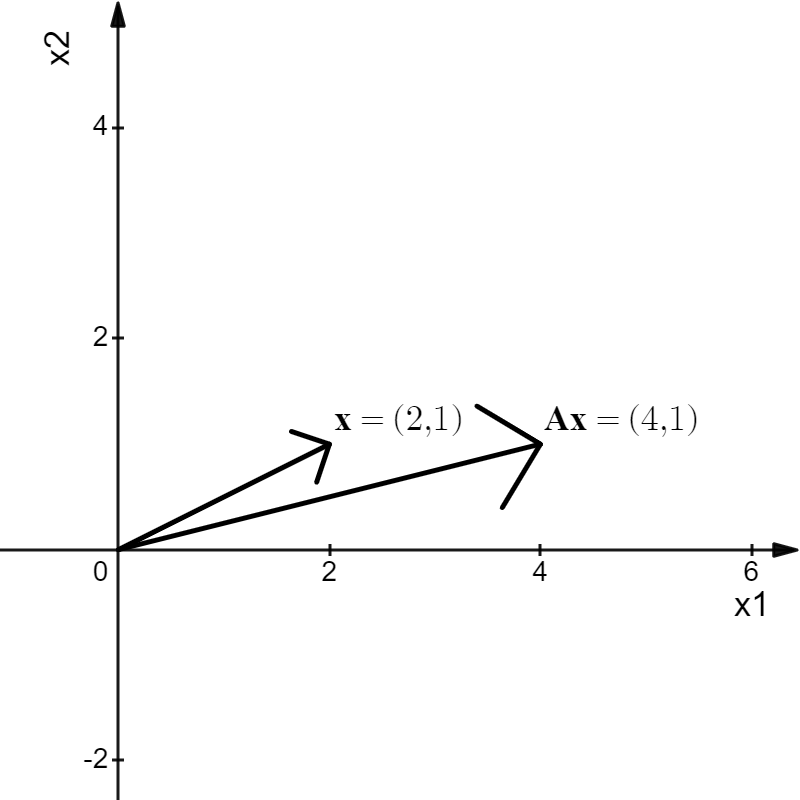
\includegraphics[width=0.5\linewidth]{images/lt} 

}

\caption{A linear transformation}\label{fig:lt1}
\end{figure}

Note that

\[\mathbf{A}\mathbf{e}_1=\begin{bmatrix} 1 & 2 \\-1 & 3\end{bmatrix}\begin{bmatrix}1\\0\end{bmatrix}=\begin{bmatrix}1\\-1\end{bmatrix},\]

which is the first column of \(\mathbf{A},\) while

\[\mathbf{A}\mathbf{e}_2=\begin{bmatrix} 1 & 2 \\-1 & 3\end{bmatrix}\begin{bmatrix}0\\1\end{bmatrix}=\begin{bmatrix}2\\3\end{bmatrix},\]

which is the second column of \(\mathbf{A}.\)

In general, if \(\mathbf{A}\) is any matrix and \(\mathbf{e}_i\) is the standard basis vector of appropriate length, then \(\mathbf{A}\mathbf{e}_i=\mathbf{a}_i,\) the \(i\)th column of \(\mathbf{A}\)!

Now consider the product

\[\mathbf{A}\mathbf{x}=\begin{bmatrix}1& -1\\2&4\end{bmatrix}\begin{bmatrix}-1\\2\end{bmatrix}=\begin{bmatrix}-3\\6\end{bmatrix}.\]

For this matrix/vector pair, we have \(\mathbf{A}\mathbf{x}=3\mathbf{x}.\) Multiplication by \(\mathbf{A}\) stretches this particular vector by a factor of \(3\). This doesn't happen with every vector. Indeed,

\[\mathbf{A}\mathbf{e}_1=\begin{bmatrix}1\\2\end{bmatrix}.\]

The vector \(\mathbf{x}=\begin{bmatrix}-1\\2\end{bmatrix}\) is what we call an \emph{eigenvector} for the matrix \(\mathbf{A},\) and the scaling factor 3 is called an \emph{eigenvalue} of \(\mathbf{A}.\)

\begin{defbox}

\begin{definition}
Let \(\mathbf{A}\) be an \(n\times n\) (square) matrix, and let \(\mathbf{x}\) be a nonzero vector such that \(\mathbf{A}\mathbf{x}=\lambda \mathbf{x}\) for some scalar \(\lambda\). Then \(\mathbf{x}\) is an \textbf{eigenvector}\index{Eigenvector} of \(\mathbf{A}\) with corresponding \textbf{eigenvalue}\index{Eigenvalue} \(\lambda\).
\end{definition}

\end{defbox}

Some notes:

\begin{enumerate}
\def\labelenumi{\arabic{enumi}.}
\item
  While the zero vector satisfies \(\mathbf{A0}=\mathbf{0}\) for matrices \(\mathbf{A},\) we never call it an eigenvector.
\item
  Eigenvectors aren't unique. For instance, if \(\mathbf{A}\mathbf{x}=\lambda \mathbf{x}\), and \(r\) is any nonzero constant, then
  \[\mathbf{A}(r\mathbf{x})=r\mathbf{A}\mathbf{x}=r\lambda \mathbf{x}=\lambda(r\mathbf{x}),\]
  so any nonzero multiple of an eigenvector is also an eigenvector for the same eigenvalue. Some applications use eigenvectors of magnitude 1, while others use eigenvalues whose entries add up to 1.
\end{enumerate}

Now that we've defined eigenvectors and eigenvalues, we need to figure out how to find them.

Eigenvectors and eigenvalues satisfy the equation

\[\mathbf{A}\mathbf{x}=\lambda\mathbf{x}.\]

With a little rearrangement, and using the trick \(\mathbf{I}\mathbf{x}=\mathbf{x}\), we get the following:

\begin{align*}
    \mathbf{A}\mathbf{x}&=\lambda \mathbf{x}\\
    \mathbf{A}\mathbf{x}-\lambda\mathbf{x}&=\mathbf{0}\\
    \mathbf{A}\mathbf{x}-\lambda \mathbf{I}\mathbf{x}&=\mathbf{0}\\
    (\mathbf{A}-\lambda \mathbf{I})\mathbf{x}&=\mathbf{0}.
\end{align*}

If \(\mathbf{A}\) is a square \(n\times n\) matrix, then \(\mathbf{B}=\mathbf{A}-\lambda\mathbf{I}\) is also an \(n\times n\) matrix. Remember that for a square matrix \(\mathbf{B},\)

\[\mathbf{B}\mathbf{x}=\mathbf{0}\]

has a nontrivial solution if and only if \(\det \mathbf{B}=0.\) The matrix \(\mathbf{A}\) will have the eigenvalue \(\lambda\) if and only if

\[
\det(\mathbf{A}-\lambda\mathbf{I})=0. \label{eq:chareq}
\]

This is the \emph{characteristic equation}\index{Characteristic equation} for the matrix \(\mathbf{A}.\) Any nontrivial solution to the characteristic equation will be an eigenvector corresponding to the eigenvalue \(\lambda.\)

To sum up, we have the following.

\begin{theorembox}

\begin{theorem}
The value \(\lambda\) is an eigenvalue for the \(n\times n\) matrix \(\mathbf{A}\) if and only if

\[\det(\mathbf{A}-\lambda\mathbf{I})=0.\]

Corresponding eigenvectors are nonzero solutions to

\[(\mathbf{A}-\lambda \mathbf{I})\mathbf{x}=\mathbf{0}.\]
\end{theorem}

\end{theorembox}

For a given matrix \(\mathbf{A},\) \(\det(\mathbf{A}-\lambda\mathbf{I})\) is a polynomial in \(\lambda\), called the \emph{characteristic polynomial}\index{Characteristic polynomial} of \(\mathbf{A}.\)

\begin{examplebox}

\begin{example}
\protect\hypertarget{exm:fstev}{}\label{exm:fstev}Let's find eigenvalues and eigenvectors for the matrix

\[\mathbf{A}=\begin{bmatrix}1 & -1\\2 & 4\end{bmatrix}.\]

We have

\[\mathbf{A}-\lambda \mathbf{I}=\begin{bmatrix}1 & -1\\2 & 4\end{bmatrix}-\begin{bmatrix}\lambda & 0\\0 & \lambda\end{bmatrix}=\begin{bmatrix}1-\lambda & -1\\2 & 4-\lambda\end{bmatrix}.\]

Then

\begin{align*}
\det(\mathbf{A}-\lambda \mathbf{I})&=(1-\lambda)(4-\lambda)-(-1)(2) \\
&=4-\lambda-4\lambda+\lambda^2+2\\
&=\lambda^2-5\lambda+6=(\lambda-2)(\lambda-3).
\end{align*}

The characteristic equation \(\det(\mathbf{A}-\lambda \mathbf{I})=0\) for this matrix is

\[(\lambda-2)(\lambda-3)=0.\]

The eigenvalues are \(\lambda_1=3\) and \(\lambda_2=2\). (Let's write them in decreasing order.) Now that we know the eigenvalues, we can solve for the corresponding eigenvectors. We will start with \(\lambda_1=3\). A corresponding eigenvector must satisfy

\[(\mathbf{A}-3\mathbf{I})\mathbf{x}=\mathbf{0}.\]

With

\[\mathbf{A}=\begin{bmatrix}1 & -1\\2 & 4\end{bmatrix},\]

\[\mathbf{A}-3\mathbf{I}=\begin{bmatrix}1-3 & -1 \\2 & 4-3\end{bmatrix}=\begin{bmatrix}-2 & -1 \\2 & 1\end{bmatrix}.\]

To solve \((\mathbf{A}-3\mathbf{I})\mathbf{x}=\mathbf{0}\), we reduce:

\[\left[\begin{array}{rr|r}-2 & -1 & 0\\2 & 1 & 0\end{array}\right] \leadsto \left[\begin{array}{rr|r} 1 & 1/2 & 0\\0 & 0 & 0\end{array}\right].\]

Any vector \(\mathbf{x}=(x_1,x_2)\) that satisfies \(x_1=-\frac{1}{2}x_2\) will be an eigenvector. For instance, \(\mathbf{x}=(-1,2)\) is the one we saw in the example. We'll let \(\mathbf{x}=\mathbf{x}_1=(-1,2)\) be our eigenvector corresponding to \(\lambda_1=3.\)

Note that in

\[\mathbf{A}-3\mathbf{I}=\begin{bmatrix}-2 & -1 \\2 & 1\end{bmatrix},\]

the rows are multiples of each other. We can actually use either row to find a relationship between the coordinates, without having to row reduce. (This only works for \(2\times 2\) matrices.) The second row tells us that \(2x_1+x_2=0\), or \(x_2=-2x_1\). If we let \(x_1=1\), we get \(x_2=-2\), for an eigenvector of \(\mathbf{x}_1=(1,-2)\), which is a multiple of the one we observed earlier.

To sum up, for \(2\times 2\) matrices, once we've found \(\mathbf{A}-\lambda \mathbf{I}\), we can jump straight to the eigenvector.

Now let's find an eigenvector corresponding to \(\lambda_2=2\). We have

\[\mathbf{A}-2\mathbf{I}=\begin{bmatrix}1-2 & -1 \\2 & 4-2\end{bmatrix}=\begin{bmatrix}-1 & -1 \\2 & 2\end{bmatrix}.\]

The first row tells us that \(-x_1-x_2=0,\) or \(x_2=-x_1\). The vector \(\mathbf{x}_2=(1,-1)\) works. Let's check:

\[\mathbf{A}\mathbf{x}_2=\begin{bmatrix}1 & -1\\2 & 4\end{bmatrix}\begin{bmatrix}1\\-1\end{bmatrix}=\begin{bmatrix}2\\-2\end{bmatrix}=2\mathbf{x}_2\checkmark.\]
\end{example}

\end{examplebox}

\subsection*{Eigenvalues and Eigenvectors in R}\label{eigenvalues-and-eigenvectors-in-r}
\addcontentsline{toc}{subsection}{Eigenvalues and Eigenvectors in R}

We can use R to find eigenvalues and eigenvectors via the \texttt{eigen} function from the base package. If they are all real numbers, the eigenvalues will be listed in descending order. The corresponding eigenvectors are listed in the same order. The eigenvectors are scaled so that the have magnitude 1.

\begin{Shaded}
\begin{Highlighting}[]
\NormalTok{A }\OtherTok{\textless{}{-}} \FunctionTok{matrix}\NormalTok{(}\FunctionTok{c}\NormalTok{(}\DecValTok{1}\NormalTok{,}\DecValTok{2}\NormalTok{,}\SpecialCharTok{{-}}\DecValTok{1}\NormalTok{,}\DecValTok{4}\NormalTok{), }\AttributeTok{nrow =} \DecValTok{2}\NormalTok{)}
\NormalTok{A}
\end{Highlighting}
\end{Shaded}

\begin{verbatim}
##      [,1] [,2]
## [1,]    1   -1
## [2,]    2    4
\end{verbatim}

\begin{Shaded}
\begin{Highlighting}[]
\FunctionTok{eigen}\NormalTok{(A)}
\end{Highlighting}
\end{Shaded}

\begin{verbatim}
## eigen() decomposition
## $values
## [1] 3 2
## 
## $vectors
##            [,1]       [,2]
## [1,]  0.4472136 -0.7071068
## [2,] -0.8944272  0.7071068
\end{verbatim}

If you give a name to the \texttt{eigen} output, it makes it a little easier to extract the eigenvectors.

\begin{Shaded}
\begin{Highlighting}[]
\NormalTok{A.ev }\OtherTok{\textless{}{-}} \FunctionTok{eigen}\NormalTok{(A)}
\NormalTok{evectors }\OtherTok{\textless{}{-}}\NormalTok{ A.ev}\SpecialCharTok{$}\NormalTok{vectors}
\NormalTok{evectors}
\end{Highlighting}
\end{Shaded}

\begin{verbatim}
##            [,1]       [,2]
## [1,]  0.4472136 -0.7071068
## [2,] -0.8944272  0.7071068
\end{verbatim}

\begin{Shaded}
\begin{Highlighting}[]
\NormalTok{evectors[,}\DecValTok{1}\NormalTok{]}
\end{Highlighting}
\end{Shaded}

\begin{verbatim}
## [1]  0.4472136 -0.8944272
\end{verbatim}

\begin{Shaded}
\begin{Highlighting}[]
\NormalTok{evectors[,}\DecValTok{2}\NormalTok{]}
\end{Highlighting}
\end{Shaded}

\begin{verbatim}
## [1] -0.7071068  0.7071068
\end{verbatim}

Another option for finding eigenvalues and eigenvectors for small matrices is \href{https://www.wolframalpha.com/}{WolframAlpha.com}. After you enter a matrix, the engine will spit out several of its properties. As of this writing, the Desmos.com matrix calculator does not do eigenvalue/eigenvector computations.

\subsection*{Higher dimensional matrices}\label{higher-dimensional-matrices}
\addcontentsline{toc}{subsection}{Higher dimensional matrices}

The characteristic polynomial for a \(2\times 2\) matrix is a quadratic polynomial. The characteristic polynomial for an \(n\times n\) matrix will be an \(n\)th degree polynomial, which makes it harder or impossible to do by hand.

\begin{examplebox}

\begin{example}
Find the eigenvalues and eigenvectors for

\[\mathbf{A}=\begin{bmatrix}-1 & 2 & 0\\2 & 0 & 2\\0 & 2 & 1\end{bmatrix}.\]

We have

\begin{align*}\det(\mathbf{A}-\lambda\mathbf{I})&=\begin{vmatrix}-1-\lambda & 2 & 0\\2 & -\lambda & 2\\0 & 2 & 1-\lambda\end{vmatrix}\\
&=-\lambda^3+9\lambda\\
&=-\lambda(\lambda^2-9)\\
&=-\lambda(\lambda+3)(\lambda-3)
\end{align*}

The eigenvalues are \(\lambda_1=3,\lambda_2=0,\) and \(\lambda_3=-3.\)

For \(\lambda_1=3,\) we reduce.

\begin{align*}
\left[\begin{array}{ccc|c}-1-3 & 2 & 0&0\\2 & 0-3 & 2&0\\0 & 2 & 1-3&0\end{array}\right]&=\left[\begin{array}{ccc|c} -4 & 2 & 0&0\\2 & -3 & 2&0\\0 & 2 & -2&0\end{array}\right] \\
&\leadsto \left[\begin{array}{ccc|c} 1 & 0 & -1/2 &0\\0 & 1 & -1&0\\0 & 0 & 0&0\end{array}\right]
\end{align*}

We get that \(x_3\) is free, \(x_1=\frac{1}{2}x_3\) and \(x_2=x_3\). Setting \(x_3=2\) gives us \(\mathbf{x}_1=(1,2,2).\)

For \(\lambda_2=0,\) we get the following.

\[
\left[\begin{array}{ccc|c}-1 & 2 & 0&0\\2 & 0 & 2&0\\0 & 2 & 1&0\end{array}\right]\leadsto \left[\begin{array}{ccc|c} 1 & 0 & 1 &0\\0 & 1 & 1/2&0\\0 & 0 & 0&0\end{array}\right]
\]

Again, with \(x_3\) free, we get \(x_1=-x_3\) and \(x_2=-\frac{1}{2}x_3.\) Setting \(x_3=2\) gives us an eigenvector of \(\mathbf{x}_2=(-2,1,2)\).

For \(\lambda_3=-3,\) we have this.

\begin{align*}
\left[\begin{array}{ccc|c}-1+3 & 2 & 0&0\\2 & 0+3 & 2&0\\0 & 2 & 1+3&0\end{array}\right]&=\left[\begin{array}{ccc|c} 2 & 2 & 0&0\\2 & 3 & 2&0\\0 & 2 & 4&0\end{array}\right] \\
&\leadsto \left[\begin{array}{ccc|c} 1 & 0 & -2 &0\\0 & 1 & 2&0\\0 & 0 & 0&0\end{array}\right]
\end{align*}

The relationships are \(x_1=2x_3\) and \(x_2=-2x_3\), so letting \(x_3=2\) gives us our final eigenvector of \(\mathbf{x}_3=(2,-2,1).\)
\end{example}

\end{examplebox}

\section{Special Cases and Complications}\label{special-cases-and-complications}

There are some matrices for which it is easy to find eigenvalues.

\subsection*{Diagonal and triangular matrices}\label{diagonal-and-triangular-matrices}
\addcontentsline{toc}{subsection}{Diagonal and triangular matrices}

We talked about diagonal and triangular matrices in Section \ref{dets}. It is easy to find their eigenvalues.\index{Diagonal matrix!eigenvalues of}\index{Triangular matrix!eigenvalues of}

\begin{examplebox}

\begin{example}
\protect\hypertarget{exm:tmev}{}\label{exm:tmev}Find the eigenvalues and eigenvectors for \(\mathbf{A},\) where

\[\mathbf{A}=\begin{bmatrix}2 & 3\\0 & 5\end{bmatrix}.\]

Note that

\[\det(\mathbf{A}-\lambda \mathbf{I})=\begin{vmatrix}2-\lambda & 3\\0 & 5-\lambda\end{vmatrix}=(2-\lambda)(5-\lambda),\]

so the eigenvalues are 2 and 5, the entries on the diagonal.
\end{example}

\end{examplebox}

When we subtract \(\lambda\) from the diagonal, a triangular or diagonal matrix stays triangular or diagonal, and the determinant is the product of the diagonal entries. This gives us the following theorem.

\begin{theorembox}

\begin{theorem}
Let \(\mathbf{A}\) be an \(n\times n\) diagonal, upper triangular, or lower triangular matrix. The eigenvalues of \(\mathbf{A}\) are the entries on the diagonal of \(\mathbf{A}.\)
\end{theorem}

\end{theorembox}

This means that we can immediately read off the eigenvalues for these special matrices.

Returning to Example \ref{exm:tmev}, we should find the eigenvectors. We'll start with \(\lambda_2=2.\) First, remember that the columns of a matrix tell us what happen to the standard basis vectors. Note that

\[\mathbf{A}\begin{bmatrix}1 \\0\end{bmatrix}=\begin{bmatrix}2\\0\end{bmatrix},\]

so \(\mathbf{x}_2=\begin{bmatrix}1\\0\end{bmatrix}\) is an eigenvector corresponding to \(\lambda_2=2.\)

We still need to find the eigenvector corresponding to \(\lambda_1=5.\) This one takes a little more work.

\[\left[\begin{array}{cc|c} 2-5 & 3 & 0\\0 & 5-5 & 0\end{array}\right]=\left[\begin{array}{rr|r}-3 & 3& 0\\0 & 0 & 0\end{array}\right].\]

The first row tells us that \(3x_2=3x_1\) or \(x_2=x_1\). Thus \(\mathbf{x}_1=\begin{bmatrix}1\\1\end{bmatrix}\) is an eigenvector corresponding to \(\lambda_1=5.\)

Note that the standard basis vectors are all eigenvectors for diagonal matrices. For example,

\[\begin{bmatrix} 2 & 0 & 0\\ 0 & 3 & 0\\0 & 0 & 5\end{bmatrix}\begin{bmatrix}0\\1\\0\end{bmatrix}=\begin{bmatrix}0 \\3\\0\end{bmatrix}.\]

\subsection*{The trace}\label{the-trace}
\addcontentsline{toc}{subsection}{The trace}

For a generic \(2\times 2\) matrix \(\mathbf{A},\) the characteristic polynomial is:

\begin{align*} 
\begin{vmatrix} a-\lambda & b\\c & d-\lambda\end{vmatrix}&=(a-\lambda)(d-\lambda)-bc\\
&=ad-a\lambda-d\lambda+\lambda^2-bc\\
&=\lambda^2-(a+d)\lambda+(ad-bc).
\end{align*}

Suppose the eigenvalues are \(\lambda_1\) and \(\lambda_2\). Then the characteristic polynomial is

\[(\lambda-\lambda_1)(\lambda-\lambda_2)=\lambda^2-(\lambda_1+\lambda_2)\lambda+\lambda_1\lambda_2.\]

Matching coefficients gives us the following:

\[\lambda_1+\lambda_2=a+d\text{ and }\lambda_1\lambda_2=ad-bc.\]

First note that \(\lambda_1\lambda_2=ad-bc=\det \mathbf{A}\). The determinant of a \(2\times 2\) matrix is the product of the eigenvalues.

The \(\lambda\)-coefficient is \(-(\lambda_1+\lambda_2)=-(a+d)\), and \(a+d\) is the sum of the diagonal entries. This is called the \emph{trace} of a matrix.

\begin{defbox}

\begin{definition}
Let \(\mathbf{A}\) be an \(n\times n\) matrix. The \textbf{trace}\index{Trace} of \(\mathbf{A},\) denoted \(\text{tr }\mathbf{A}\), is the sum of the diagonal entries of \(\mathbf{A}.\)
\end{definition}

\end{defbox}

For a \(2\times 2\) matrix, the trace is the sum of the eigenvalues. This relationship -- and the relationship between the eigenvalues and the determinant -- also hold for larger matrices

\begin{theorembox}

\begin{theorem}
Let \(\mathbf{A}\) be an \(n\times n\) matrix with eigenvalues \(\lambda_1,\lambda_2,\dots,\lambda_n\), including repetitions. Then

\[\det \mathbf{A}= \lambda_1\lambda_2\cdots \lambda_n,\]

and

\[\text{tr } \mathbf{A}= \lambda_1+\lambda_2+\cdots+\lambda_n.\]
\end{theorem}

\end{theorembox}

Note that these are somewhat obvious for diagonal and triangular matrices, but are also true for all square matrices.

\begin{examplebox}

\begin{example}
\protect\hypertarget{exm:ndnt}{}\label{exm:ndnt}Find a nondiagonal/nontriangular \(2\times 2\) matrix with eigenvalues \(\lambda_1=5\) and \(\lambda_2=-1\).

Let \(\mathbf{A}=\begin{bmatrix}a & b\\c& d\end{bmatrix}.\) We know that \(\text{tr }\mathbf{A}=\lambda_1+\lambda_2=5+-1=4.\) We can pick any pair of diagonal entries that add up to 4 (other than 5 and \(-1\)). Let's choose \(a=2\) and \(d=2\). The determinant is \(\lambda_1\lambda_2=5(-1)=-5.\) With \(a=d=2, \det\mathbf{A}=4-bc=-5,\) so \(bc=9.\) We can choose any pair of numbers whose product is 9. Let's let \(b=c=3.\) Then our matrix is

\[\mathbf{A}=\begin{bmatrix}2& 3\\3 & 2\end{bmatrix}.\]
\end{example}

\end{examplebox}

\subsection*{Complications}\label{complications}
\addcontentsline{toc}{subsection}{Complications}

So far, all of our examples have involved matrices with real, distinct eigenvalues. Because we are dealing with solutions to polynomial equations, things can become messier.

As an example, note that \(\mathbf{A}=\begin{bmatrix}2 & 0\\0 & 2\end{bmatrix}\) and \(\mathbf{B}=\begin{bmatrix}2 & 3\\0 & 2\end{bmatrix}\) both have the repeated eigenvalue 2. Since \(\mathbf{A}\) is diagonal, \(\mathbf{e}_1\) and \(\mathbf{e}_2\) are two linearly independent eigenvectors for it. (In fact, any nonzero vector in \(\mathbb{R}^2\) is an eigenvector, since \(\mathbf{A}=2\mathbf{I}\).)

For \(\mathbf{B},\) \(\mathbf{e}_1\) is also an eigenvector, but \(\mathbf{e}_2\) isn't. If we try to solve for one in the normal way,

\[\left[\begin{array}{cc|c}2-2 & 3 & 0\\0 & 2-2 & 0\end{array}\right]=\left[\begin{array}{cc|c}0 & 3& 0\\0 & 0 & 0\end{array}\right],\]

we get that \(x_2=0\), so we only have a single linearly independent eigenvector \(\mathbf{e}_1=(1,0)\). In this case, \(\lambda=2\) is what we call a \emph{deficient}\index{Deficient eigenvalue} eigenvalue.

It's also possible for a matrix to have complex-valued eigenvalues. For example, with \(\text{tr }\mathbf{A}=-3,\det \mathbf{A}=5,\)

\[\mathbf{A}=\begin{bmatrix} -1 & -3\\1 & -2\end{bmatrix}\]
has characteristic equation

\[\lambda^2+3\lambda+5=0,\]

so the eigenvalues are

\[\lambda=\frac{-3\pm \sqrt{3^2-4\cdot 1\cdot 5}}{2}=\frac{-3\pm \sqrt{-11}}{2}=-\frac{3}{2}\pm i\frac{\sqrt{11}}{2}.\]

Fortunately, for our applications, the matrices will either only have all real eigenvalues or we'll only need the real eigenvalues.

\subsection*{Eigenvalues of a transpose}\label{eigenvalues-of-a-transpose}
\addcontentsline{toc}{subsection}{Eigenvalues of a transpose}

How do the eigenvalues of a matrix and its transpose compare? Note that, since \(\mathbf{I}^T=\mathbf{I},\)

\begin{align*}
\det (\mathbf{A}^T-\lambda \mathbf{I})&=\det (\mathbf{A}^T-\lambda \mathbf{I}^T)\\
&=\det (\mathbf{A}-\lambda \mathbf{I})^T\\
&=\det (\mathbf{A}-\lambda \mathbf{I}),
\end{align*}

so \(\mathbf{A}\) and \(\mathbf{A}^T\) have the same characteristic polynomial. Since they have the same characteristic polynomial, they have the same eigenvalues. They don't necessarily have the same eigenvectors, however.

\begin{theorembox}

\begin{theorem}
Let \(\mathbf{A}\) be a square matrix. Then \(\mathbf{A}\) and \(\mathbf{A}^T\) have the same eigenvalues.
\end{theorem}

\end{theorembox}

\subsection*{Matrix powers}\label{matrix-powers}
\addcontentsline{toc}{subsection}{Matrix powers}

Suppose that \(\mathbf{A}\) is an \(n\times n\) matrix, with eigenvalue \(\lambda\) and corresponding eigenvector \(\mathbf{x}\). Then

\begin{align*}
    \mathbf{A}\mathbf{x}&=\lambda \mathbf{x}\\
\mathbf{A}^2\mathbf{x}&=\mathbf{A}(\mathbf{A}\mathbf{x})=\mathbf{A}(\lambda \mathbf{x})=\lambda(\mathbf{A}\mathbf{x})=\lambda(\lambda \mathbf{x})=\lambda^2\mathbf{x}\\
\vdots & \\
\mathbf{A}^n\mathbf{x}&=\lambda^n \mathbf{x}.
\end{align*}

So:

\begin{enumerate}
\def\labelenumi{\arabic{enumi}.}
\item
  Eigenvectors of \(\mathbf{A}\) are eigenvectors of \(\mathbf{A}^n\) with eigenvalues \(\lambda^n, n=2,3,\dots\)
\item
  This makes it easy to calculate \(\mathbf{A}^n\mathbf{x}\) for eigenvectors. We'll take advantage of this in upcoming sections.
\end{enumerate}

\begin{examplebox}

\begin{example}
Let

\[\mathbf{A}=\begin{bmatrix} 1 & -1\\2 & 4\end{bmatrix}.\]
We know from Example \ref{exm:fstev} that \(\mathbf{x}=\begin{bmatrix}-1 \\2\end{bmatrix}\) is an eigenvector of \(\mathbf{A}\) with corresponding eigenvalue \(\lambda=3\). Then

\[\mathbf{A}^4\mathbf{x}=3^4\mathbf{x}=81\begin{bmatrix}-1\\2\end{bmatrix}=\begin{bmatrix}-81\\162\end{bmatrix}.\]
\end{example}

\end{examplebox}

\section{Application: The Leslie Matrix}\label{application-the-leslie-matrix}

In this section, we will be studying an application of eigenvalues and eigenvectors to population modeling.

Patrick Leslie described his matrix method\index{Leslie matrix} for studying discrete time, age-structured population models in 1945 \autocite{Leslie}. The model includes year-to-year survival rates as well as reproduction rates. We will start with an example.

\begin{examplebox}

\begin{example}
\protect\hypertarget{exm:Leslie1}{}\label{exm:Leslie1}Suppose a species lives at most two years, reproduces each year, and dies. We will consider the zero-year-olds, one-year-olds, and two-year-olds separately.

\begin{itemize}
\item
  Each age 0 individual has a probability of surviving to age 1 of 0.2, and produces on average 2 offspring.
\item
  Each age 1 individual has a probability of surviving to age 2 of 0.5, and produces an average of 4 offspring.
\item
  Each age 2 individual has a survival probability of 0, but produces an average of 3 offspring.
\end{itemize}

The Leslie matrix for this population looks like this:

\[\mathbf{L}=\begin{bmatrix} 2 & 4 & 3\\
0.2 & 0 & 0\\ 0 & 0.5 & 0\end{bmatrix}.\]
\end{example}

\end{examplebox}

Before we explain what we do with the matrix, we need to talk about population vectors.

Let \(N_0(t)\) represent the number of age 0 individuals at year \(t\), \(N_1(t)\) represent the number of one-year-olds, and \(N_2(t)\) is the number of two-year-olds. We can combine these populations into a single vector:

\[\mathbf{N}(t)=\begin{bmatrix}N_0(t)\\N_1(t)\\N_2(t)\end{bmatrix}.\]

For example, if we start with 10 age-zero, 20 age-1 and 20 age-2 individuals, then

\[\mathbf{N}(0)=\begin{bmatrix}10\\20\\20\end{bmatrix}.\]

To find the population distribution for the next year, we multiply \(\mathbf{N}(t)\) by \(\mathbf{L}\):

\[\mathbf{N}(1)=\mathbf{L}\,\mathbf{N}(0),\]

\[\mathbf{N}(2)=\mathbf{L}\,\mathbf{N}(1),\]

and so on. In general,

\[\mathbf{N}(t+1)=\mathbf{L}\,\mathbf{N}(t).\]

With our initial distribution of \(\mathbf{N}(0)=(10,20,20)\), the distribution one year later will be

\[\mathbf{N}(1)=\begin{bmatrix}2 & 4 & 3\\
0.2 & 0 & 0\\0 & 0.5 & 0\end{bmatrix}\begin{bmatrix}10\\20\\20\end{bmatrix}=\begin{bmatrix}160\\2\\10\end{bmatrix}.\]

Is this right? We have 20\% of the age-0 individuals surviving to age 1. Fifty percent of the 20 age-one population (10) survive to age 2. The new age-zero population is

\[2\cdot 10+4\cdot 20+3\cdot 20=20+80+60=160.\]

\emph{How it works}:

Remember that the columns of a matrix tell you what happens to the standard basis vector under multiplication. For instance,

\[\mathbf{L}\,\mathbf{e}_1=\begin{bmatrix}2&4&3\\0.2&0 & 0\\0 & 0.5 & 0\end{bmatrix}\begin{bmatrix}1\\0\\0\end{bmatrix}=\begin{bmatrix}2\\0.2\\0\end{bmatrix}.\]

A single age-0 individual will produce (on average) 2 offspring, has a probability of 0.2 of surviving to age 1, and does not contribute to the age-2 population. We can analyze the other columns in a similar manner.

We can keep going.

\[\mathbf{N}(2)=\mathbf{L}\mathbf{N}(1)=\begin{bmatrix}2&4&3\\0.2&0&0\\0&0.5&0\end{bmatrix}\begin{bmatrix}160\\2\\10\end{bmatrix}=\begin{bmatrix}358\\32\\1\end{bmatrix}.\]

Note that

\[\mathbf{N}(2)=\mathbf{L}\,\mathbf{N}(1)=\mathbf{L}(\mathbf{L}\,\mathbf{N}(0))=\mathbf{L}^2\,\mathbf{N}(0).\]

In general, \(\mathbf{N}(t)=\mathbf{L}^t\,\mathbf{N}(0)\).

Figure \ref{fig:leslie1} shows a plot of the age group populations over time.

\begin{figure}

{\centering 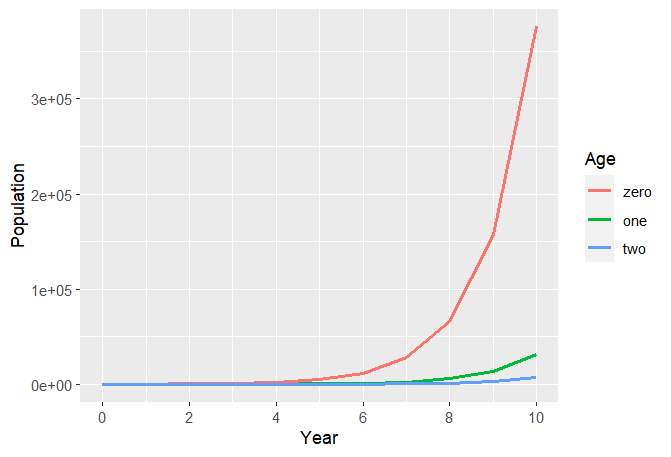
\includegraphics[width=0.75\linewidth]{images/leslie1} 

}

\caption{Population growth}\label{fig:leslie1}
\end{figure}

If we plot the age groups' share of the total population over time, something interesting happens (Fig. \ref{fig:leslie2}).

\begin{figure}

{\centering 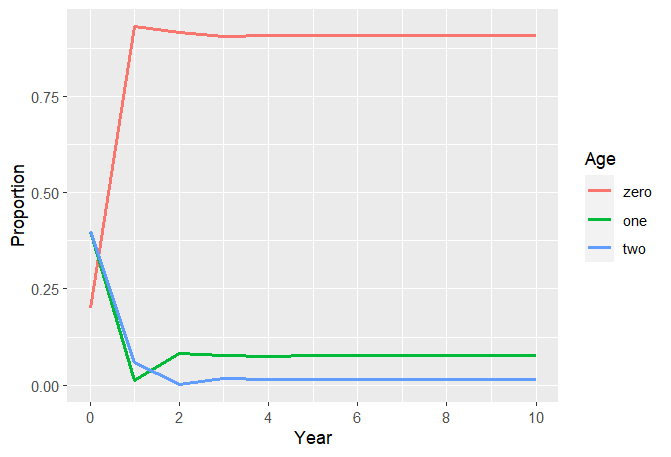
\includegraphics[width=0.75\linewidth]{images/leslie2} 

}

\caption{Proportion of total population}\label{fig:leslie2}
\end{figure}

Note that after 1 year, the age-1 population is roughly 1.16\% of the total population. Also note that the proportions seem to level off. We'll investigate this more later.

Let's talk about the general form of the Leslie matrix. Suppose a population can live to age \(m\). Then its Leslie matrix will be an \((m+1)\times(m+1)\) matrix of the form

\[\mathbf{L}=\begin{bmatrix} F_0 & F_1 & F_2 & \cdots  & F_{m-1} & F_m\\P_0 & 0 & \cdots & \cdots & \cdots  & 0\\ 0 & P_1 & 0 &\cdots & \cdots  & 0\\ \vdots & \cdots & \cdots & \cdots & \cdots & \vdots\\ 0 & \cdots & \cdots & 0 & P_{m-1} & 0\end{bmatrix},\]

where \(F_i\) is the average number of offspring that an age-\(i\) individual produces. (\(F\) is for \emph{fecundity}\index{Fecundity}), and \(P_i\) is the probability that an age-\(i\) individual survives to age \(i+1\).

Suppose a Leslie matrix \(L\) has a positive eigenvalue \(\lambda\), with a corresponding eigenvector \(\mathbf{v}\) that has nonnegative entries. Then

\[\mathbf{L}\mathbf{v}=\lambda \mathbf{v}.\]

If \(\mathbf{v}\) represents a population distribution, then in the next year, each age group's population is multiplied by the same constant, \(\lambda\). That is, the proportions will stay constant, and \(\lambda\) represents the growth rate. We'll illustrate this with a \(2\times 2\) example.

\begin{examplebox}

\begin{example}
Let

\[\mathbf{L}=\begin{bmatrix}1.4 & 3\\0.05 & 0\end{bmatrix}.\]

With \(\text{tr }\mathbf{L}=1.4\) and \(\det \mathbf{L}=-0.15\), the characteristic equation is

\[\lambda^2-1.4\lambda-0.15=0,\]

and the eigenvalues are \(\lambda_1=1.5\) and \(\lambda_2=-0.1\). Let's find an eigenvector corresponding to \(\lambda_1=1.6\):

\[\mathbf{L}-1.5\mathbf{I}=\begin{bmatrix} 1.4-1.5 & 3\\0.05 & 0-1.5\end{bmatrix}=\begin{bmatrix}-0.1 & 3\\0.05 & -1.5\end{bmatrix}.\]

The first row tells us that \(-0.1v_1+3v_2=0\) or \(v_1=30v_2\). With \(v_2=1, v_1=30\). Our eigenvector is \(\mathbf{v}=(30,1)\). Let's check:

\[\mathbf{L}\mathbf{v}=\begin{bmatrix}1.4 & 3\\0.05 & 0\end{bmatrix}\begin{bmatrix}20\\1\end{bmatrix}=\begin{bmatrix}45\\1.5\end{bmatrix}=1.5\begin{bmatrix}30\\1\end{bmatrix}.\]

We didn't find the other eigenvector, and we don't really need to know what it is. Let's just call it \(\mathbf{v}_2\). We do know that it and \(\mathbf{v}_1\) are linearly independent (why?), so they form a basis for \(\mathbb{R}^2\). Let \(\mathbf{N}(0)\) be any initial population distribution. Then for some constants \(c_1\) and \(c_2\),

\[\mathbf{N}(0)=c_1\mathbf{v}_1+c_2\mathbf{v}_2.\]

Now let's iterate:

\[\mathbf{N}(t)=\mathbf{L}^t \mathbf{N}(0)=\mathbf{L}^t(c_1 \mathbf{v}_1+c_2\mathbf{v}_2)=c_1\mathbf{L}^t\mathbf{v}_1+c_2\mathbf{L}^t\mathbf{v}_2=c_1(1.6)^t\mathbf{v}_1+c_2(-0.1)^t\mathbf{v}_2.\]

As \(t\to\infty\), the \(\mathbf{v}_2\) term will vanish, and \(\mathbf{N}(t)\approx c_1\lambda^t \mathbf{v}_1\). The populations will approach a 30:1 ratio in the long run. (We're glossing over some details here.)
\end{example}

\end{examplebox}

Will we always have this situation? For \(2\times 2\) Leslie matrices, provided a positive fraction of zero-year-olds survive, and that some group produces offspring, there will always be a real, positive eigenvalue. For \(2\times 2\) Leslie matrices, we have the following theorem.\autocite{Neuhauser}

\begin{theorembox}

\begin{theorem}

Let \(\mathbf{L}\) be a \(2\times 2\) Leslie matrix with eigenvalues \(\lambda_1\) and \(\lambda_2\).

\begin{itemize}
\tightlist
\item
  The larger eigenvalue determines the growth rate.
\item
  The eigenvector corresponding to the larger eigenvalue is a stable age distribution.
\end{itemize}

\end{theorem}

\end{theorembox}

With some added conditions that we won't get into here, the analogous result holds for larger Leslie matrices. Let's return to Example \ref{exm:Leslie1} with

\[\mathbf{L}=\begin{bmatrix} 2 & 4 & 3\\
0.2 & 0 & 0\\ 0 & 0.5 & 0\end{bmatrix}.\]

\begin{Shaded}
\begin{Highlighting}[]
\NormalTok{L }\OtherTok{\textless{}{-}} \FunctionTok{matrix}\NormalTok{(}\FunctionTok{c}\NormalTok{(}\DecValTok{2}\NormalTok{,}\FloatTok{0.2}\NormalTok{,}\DecValTok{0}\NormalTok{,}\DecValTok{4}\NormalTok{,}\DecValTok{0}\NormalTok{,}\FloatTok{0.5}\NormalTok{,}\DecValTok{3}\NormalTok{,}\DecValTok{0}\NormalTok{,}\DecValTok{0}\NormalTok{), }\AttributeTok{nrow =} \DecValTok{3}\NormalTok{)}
\NormalTok{L}
\end{Highlighting}
\end{Shaded}

\begin{verbatim}
##      [,1] [,2] [,3]
## [1,]  2.0  4.0    3
## [2,]  0.2  0.0    0
## [3,]  0.0  0.5    0
\end{verbatim}

\begin{Shaded}
\begin{Highlighting}[]
\NormalTok{ev }\OtherTok{\textless{}{-}} \FunctionTok{eigen}\NormalTok{(L)}
\NormalTok{ev}
\end{Highlighting}
\end{Shaded}

\begin{verbatim}
## eigen() decomposition
## $values
## [1]  2.3876762+0.0000000i -0.1938381+0.2967692i -0.1938381-0.2967692i
## 
## $vectors
##               [,1]                  [,2]                  [,3]
## [1,] 0.99635800+0i  0.7157844+0.0000000i  0.7157844+0.0000000i
## [2,] 0.08345839+0i -0.2208541-0.3381312i -0.2208541+0.3381312i
## [3,] 0.01747691+0i -0.2289662+0.5216492i -0.2289662-0.5216492i
\end{verbatim}

Note the complex eigenvalues and eigenvectors. The first eigenvalue is purely real, as are the components of the first eigenvector. We can use the \texttt{Re} function to strip off the \texttt{0I} terms from that eigenvector. We will also rescale it so that the terms sum to 1. Then the components will represent the long term population proportions for each age group.

\begin{Shaded}
\begin{Highlighting}[]
\NormalTok{ev1 }\OtherTok{\textless{}{-}} \FunctionTok{Re}\NormalTok{(ev}\SpecialCharTok{$}\NormalTok{vectors[,}\DecValTok{1}\NormalTok{])}
\NormalTok{ev1 }\OtherTok{\textless{}{-}}\NormalTok{ ev1}\SpecialCharTok{/}\FunctionTok{sum}\NormalTok{(ev1)}
\NormalTok{ev1}
\end{Highlighting}
\end{Shaded}

\begin{verbatim}
## [1] 0.90801430 0.07605841 0.01592729
\end{verbatim}

In the long run, the percentages of 0-, 1-, and 2-year-olds approach 90.8\%, 7.6\%, and 1.6\%, respectively.

\section{Graphs and Adjacency Matrices}\label{graphs-and-adjacency-matrices}

We're going to see a few more applications of eigenvalues and eigenvectors, but before we get to them, we need to talk about graphs.

A graph\index{Graph} involves a collection of points, called \emph{vertices}\index{Vertex! of a graph}, and lines connecting them, called \emph{edges}\index{Edge! of a graph}. Note that it can be hard to draw a graph in two dimensions without the edges intersecting. These intersections are not part of the graph, in the sense that one can't switch from one edge to another without going through a vertex.

\begin{figure}

{\centering 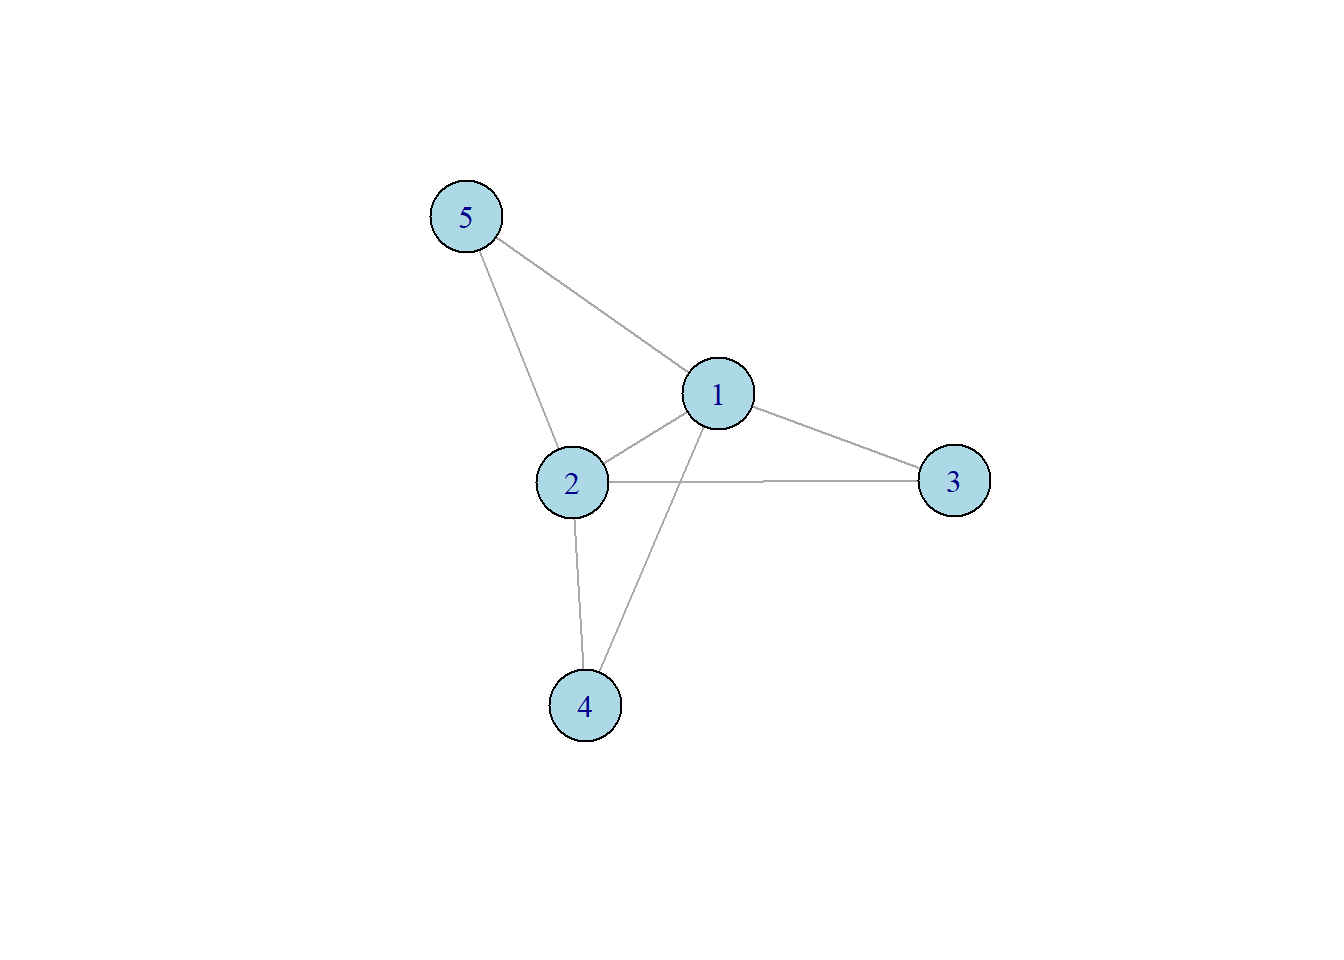
\includegraphics[width=0.75\linewidth]{_main_files/figure-latex/graph1-1} 

}

\caption{A graph}\label{fig:graph1}
\end{figure}

The following code produces the graph in \ref{fig:graph1}. It uses the \texttt{igraph} package. One note: there is a bit of randomness involved in the plot, so if you want a reproducible graph, you might want to set the seed first. See Appendix B for more sample graph code.

\begin{Shaded}
\begin{Highlighting}[]
\FunctionTok{library}\NormalTok{(igraph)}
\NormalTok{edges }\OtherTok{\textless{}{-}} \FunctionTok{c}\NormalTok{(}\DecValTok{1}\NormalTok{,}\DecValTok{2}\NormalTok{,}\DecValTok{1}\NormalTok{,}\DecValTok{3}\NormalTok{,}\DecValTok{1}\NormalTok{,}\DecValTok{5}\NormalTok{,}\DecValTok{2}\NormalTok{,}\DecValTok{3}\NormalTok{,}\DecValTok{2}\NormalTok{,}\DecValTok{4}\NormalTok{,}\DecValTok{4}\NormalTok{,}\DecValTok{1}\NormalTok{,}\DecValTok{2}\NormalTok{,}\DecValTok{5}\NormalTok{) }
\NormalTok{g }\SpecialCharTok{\textless{}} \SpecialCharTok{{-}}\FunctionTok{graph}\NormalTok{(edges, }\AttributeTok{directed =}\NormalTok{ F)}
\FunctionTok{plot}\NormalTok{(g, }\AttributeTok{vertex.size =} \DecValTok{30}\NormalTok{, }\AttributeTok{vertex.color =} \StringTok{"lightblue"}\NormalTok{)}
\end{Highlighting}
\end{Shaded}

Graphs can be used to describe road and other types of networks, and even the results of tournaments (Figs. \ref{fig:graph2},\ref{fig:graph3}).

\begin{figure}

{\centering 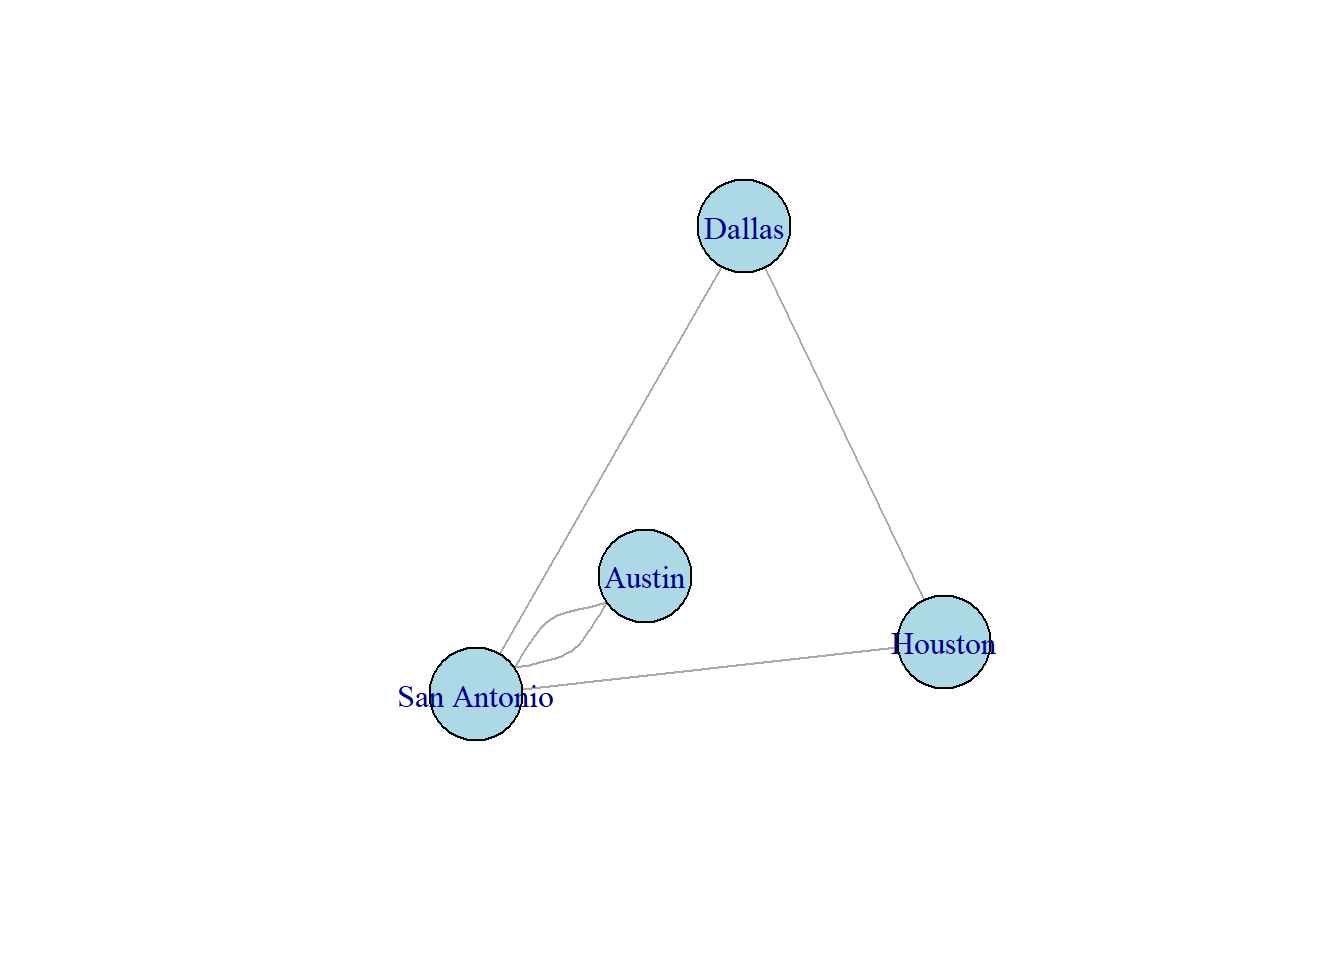
\includegraphics[width=0.75\linewidth]{_main_files/figure-latex/graph2-1} 

}

\caption{A fictional bus network}\label{fig:graph2}
\end{figure}

\begin{figure}
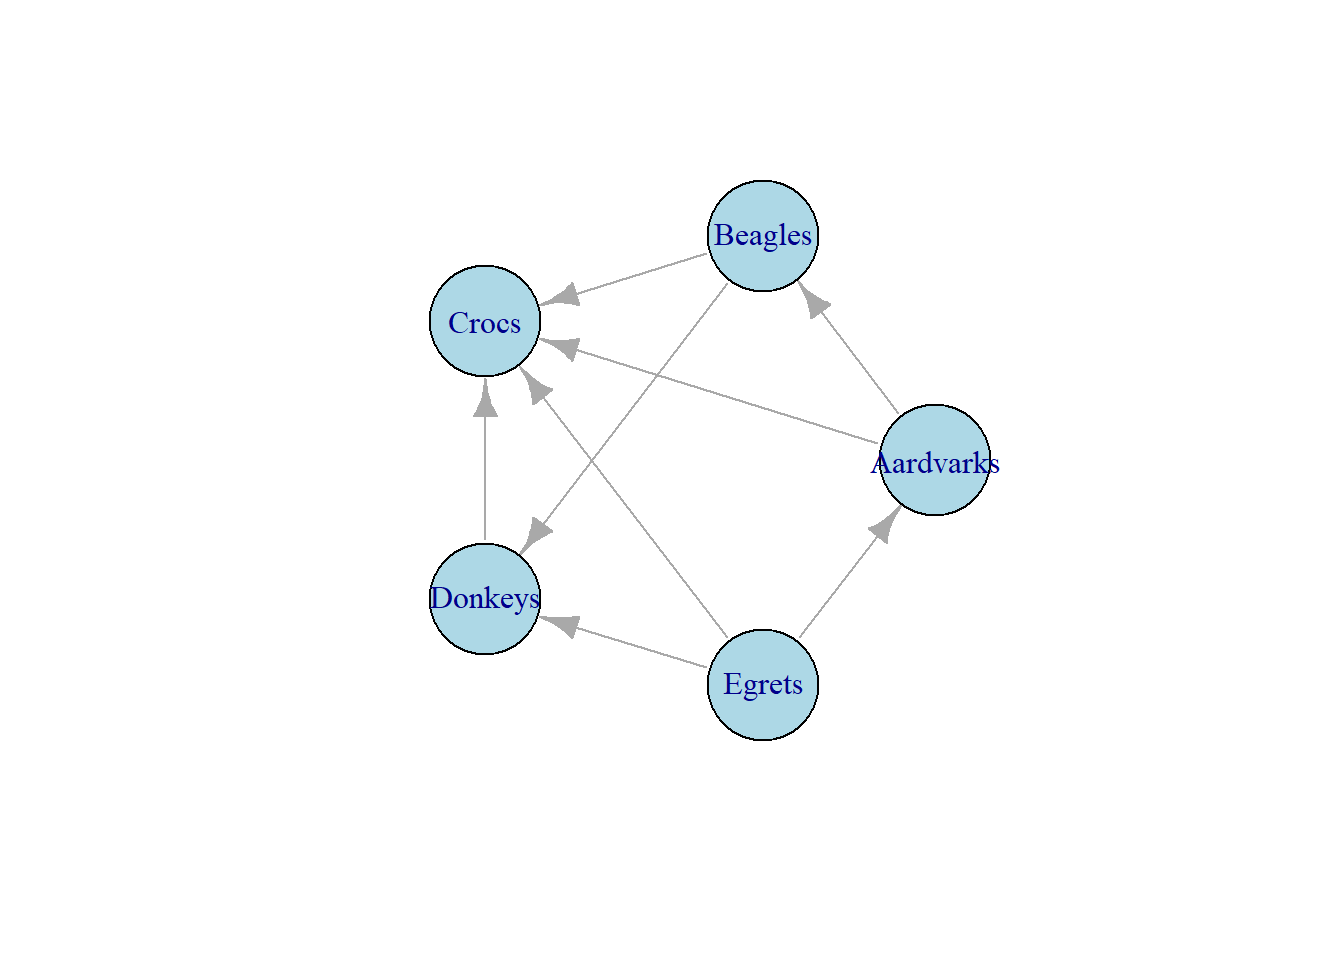
\includegraphics[width=0.75\linewidth]{_main_files/figure-latex/graph3-1} \caption{A tournament graph}\label{fig:graph3}
\end{figure}

Sometimes there is an edge from a vertex to itself, called a \emph{loop}\index{Loop}. Sometimes pairs of vertices are connected by more than one edge (Fig. \ref{fig:loopsandedges}).

\begin{figure}

{\centering 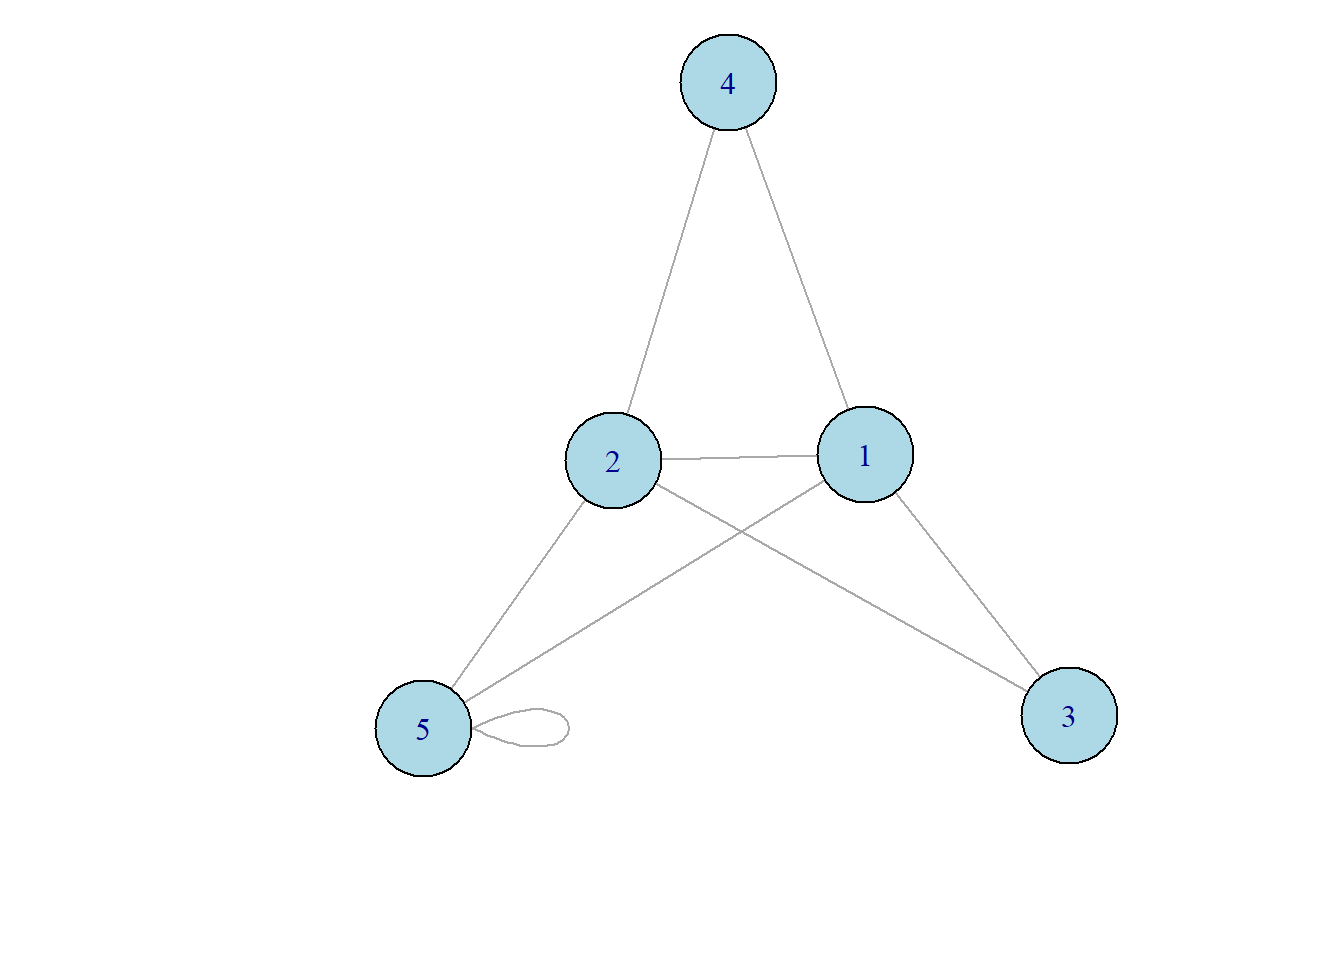
\includegraphics[width=0.45\linewidth]{_main_files/figure-latex/loopsandedges-1} 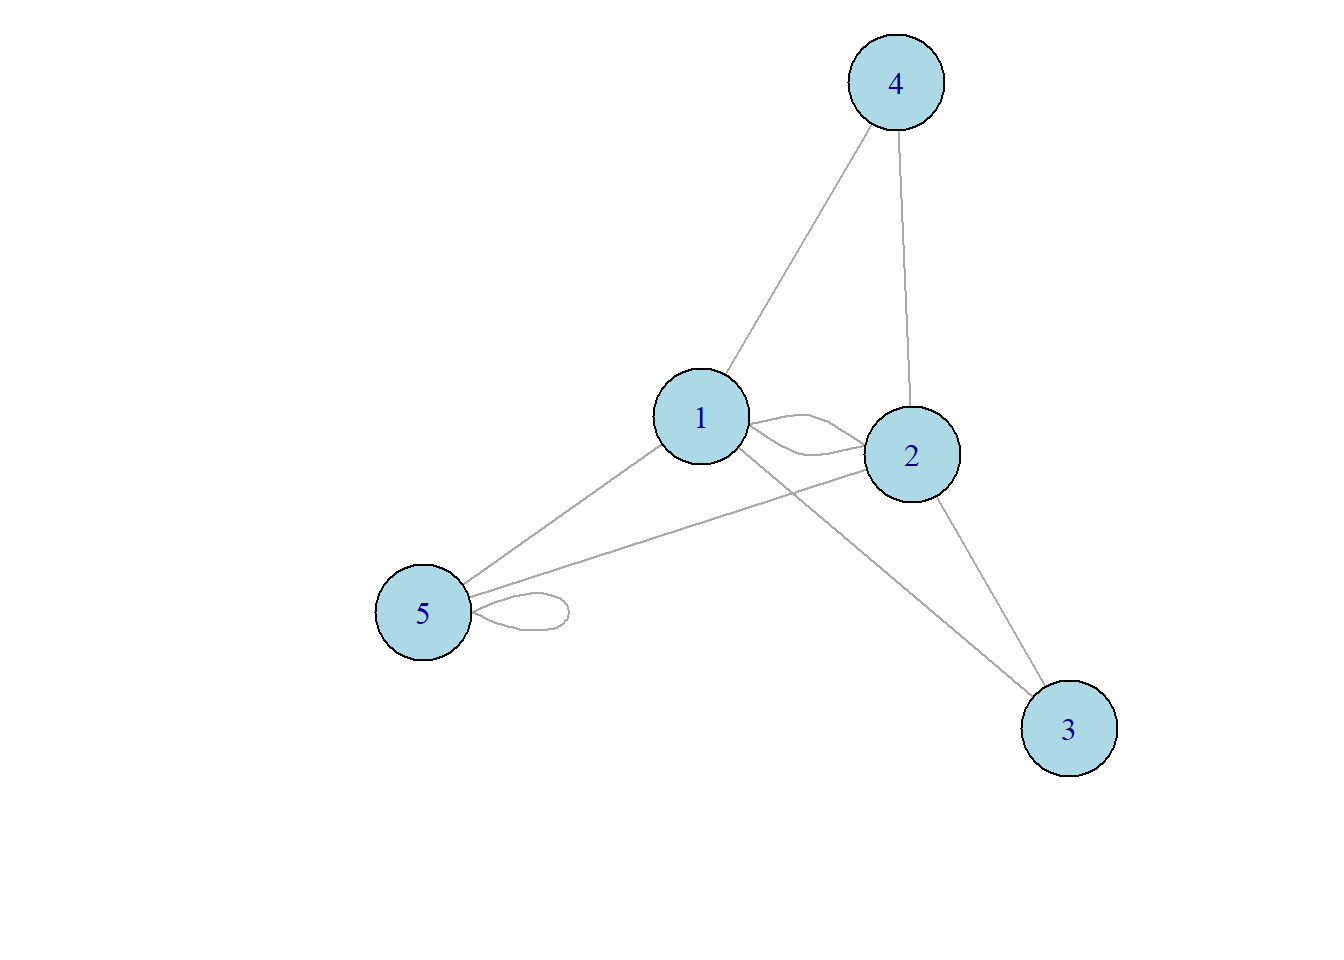
\includegraphics[width=0.45\linewidth]{_main_files/figure-latex/loopsandedges-2} 

}

\caption{Loops and multiple edges}\label{fig:loopsandedges}
\end{figure}

Sometimes the connection only goes one way. For example, if the vertices represent websites, there might be a link from one to another. In these cases, we use a \emph{directed edge}\index{Directed edge}, with the direction indicated by an arrow.

\begin{figure}

{\centering 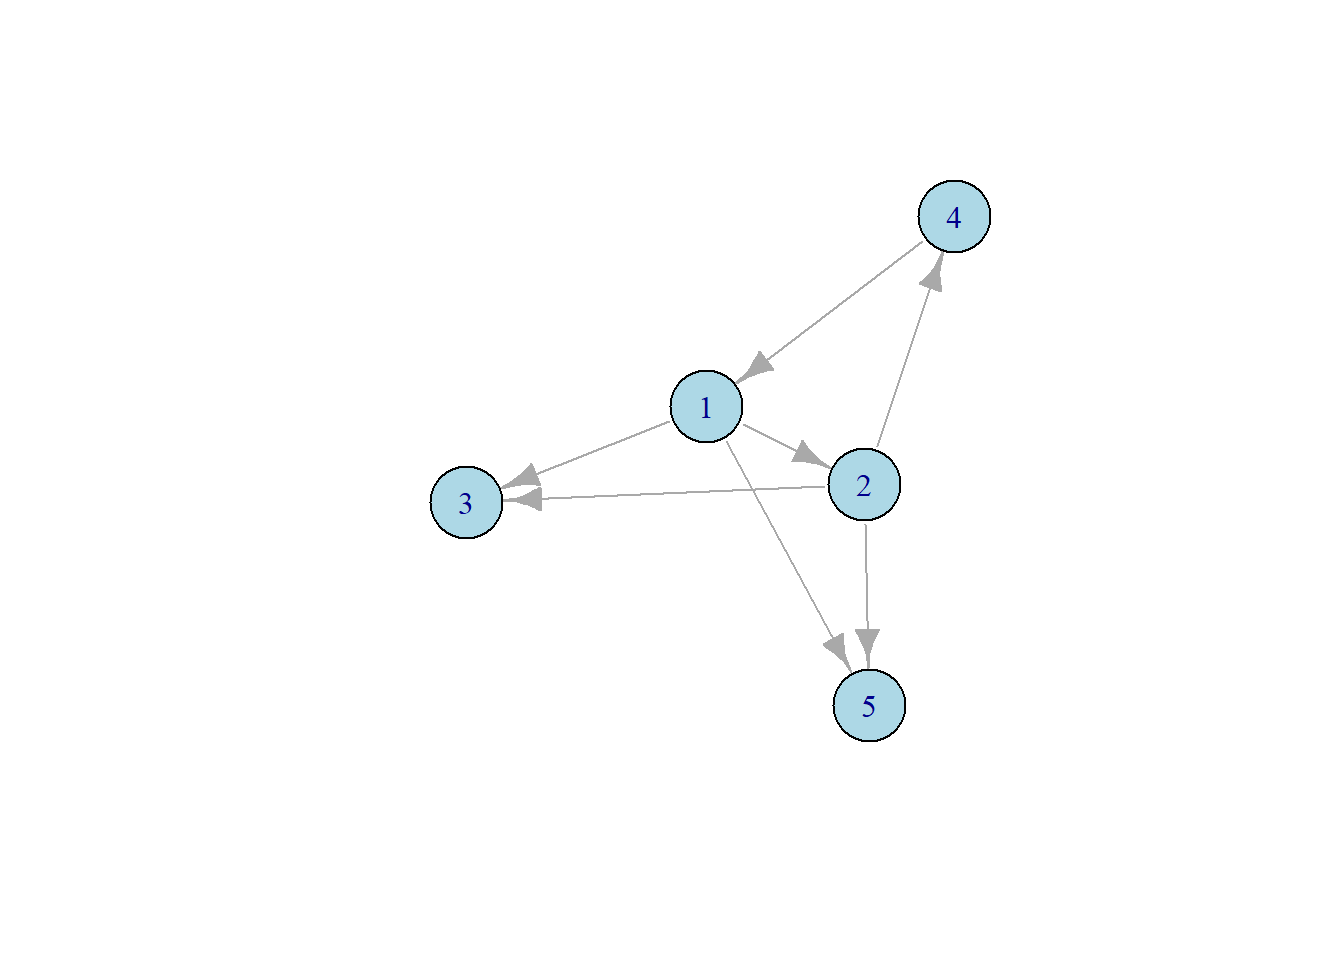
\includegraphics[width=0.75\linewidth]{_main_files/figure-latex/directed-1} 

}

\caption{A directed graph}\label{fig:directed}
\end{figure}

\subsection*{Adjacency matrices}\label{adjacency-matrices}
\addcontentsline{toc}{subsection}{Adjacency matrices}

An \emph{adjacency matrix} is a matrix that contains information about the edges and vertices of a graph.

\begin{defbox}

\begin{definition}
For an (undirected) graph with \(n\) vertices, the corresponding \textbf{adjacency matrix}\index{Adjacency matrix} is an \(n\times n\) matrix \(\mathbf{A}=[a_{ij}]\), whose \(ij\)-th entry is the number of edges connecting vertex \(i\) and vertex \(j\).
\end{definition}

\end{defbox}

Here is the adjacency matrix for the graph in Figure \ref{fig:graph1}.

\[\mathbf{A}=\begin{bmatrix}
0 & 1 & 1 & 1 &  1\\
1 & 0 & 1 & 1 & 1\\
1 & 1 & 0 & 0 & 0 \\
1 & 1 & 0 & 0 & 0 \\
1 & 1 & 0 & 0 & 0
\end{bmatrix}\]

The graph in Figure \ref{fig:loopsandedges} has the following adjacency matrix. There are two edges between vertex 1 and vertex 2, so \(a_{12}=a_{21}=2\), and the loop from vertex 5 to itself gives us \(a_{55}=1.\)

\[\begin{bmatrix}
0 & 2 & 1 & 1 &  1\\
2 & 0 & 1 & 1 & 1 \\
1 & 1 & 0 & 0 & 0 \\
1 & 1 & 0 & 0 & 0\\
1 & 1 & 0 & 0 & 1
\end{bmatrix}\]

\begin{examplebox}

\begin{example}[Bus Routes]
We saw this bus network graph before.

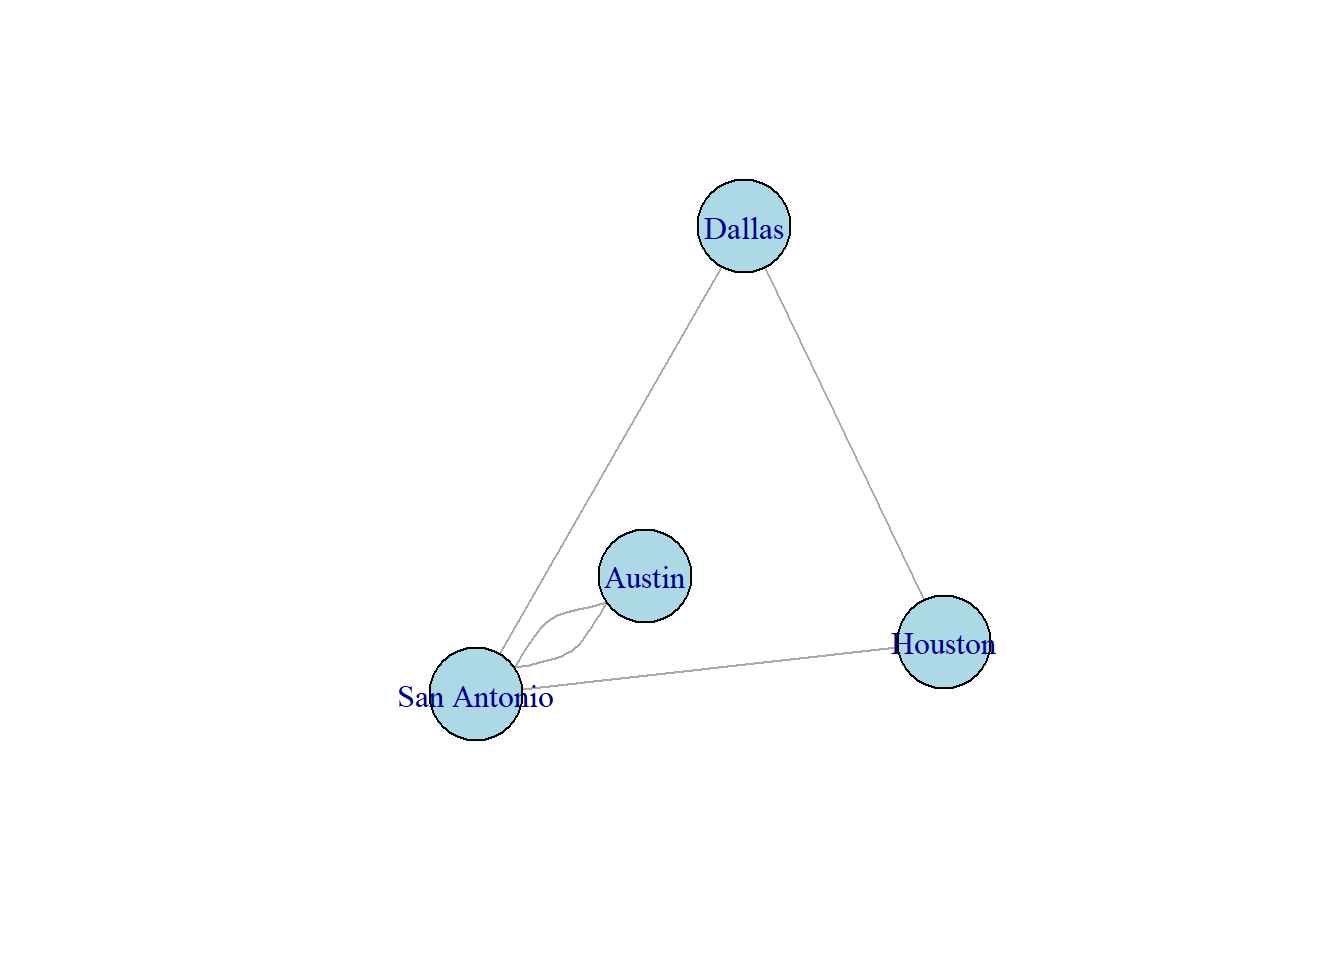
\includegraphics{_main_files/figure-latex/unnamed-chunk-17-1.pdf}

The two edges connecting Austin and San Antonio indicate two different routes. The adjacency matrix for this bus network looks like this. The vertices are numbered in alphabetical order (1 = Austin, 2 = Dallas, 3 = Houston, 4 = San Antonio).

\[\begin{bmatrix}
0 & 0 & 0 & 2\\
0 & 0 & 1 & 1\\
0 & 1 & 0 & 1\\
2 & 1 & 1 & 0
\end{bmatrix}\]

Positive integer powers of the adjacency matrix have a very nice property.

\begin{theorembox}

\begin{theorem}
Let \(\mathbf{A}\) be an adjacency matrix for a graph. If \(r\) is a positive integer, then the \(ij\)-th entry of \(\mathbf{A}^r\) is the number of routes from vertex \(i\) to vertex \(j\) that take exactly \(r\) steps.
\end{theorem}

\end{theorembox}

For the bus network, we have

\[\mathbf{A}^2=\begin{bmatrix}
4 & 2 & 2 & 0\\
2 & 2 & 1 & 1\\
2 & 1 & 2 & 1\\
0 & 1 & 1 & 6
\end{bmatrix}\]

There are two 2-step routes between Austin and Dallas, and none between Austin and San Antonio. What about three steps?

\[ \mathbf{A}^3=\begin{bmatrix}
0 & 2 & 2 & 12\\
2 & 2 & 3 & 7\\
2 & 3 & 2 & 7\\
12 & 7 & 7 & 2
\end{bmatrix}\]
\end{example}

\end{examplebox}

Why does this work? Consider the \(ij\)-th entry of \(\mathbf{A}^2\).

\[\mathbf{A}^2=\begin{bmatrix}&&&\\&&&\\a_{i1} & a_{i2} &\cdots & a_{in}\\
&&&\end{bmatrix}\begin{bmatrix}&&a_{1j}&&\\&&a_{2j}&&\\&&&&\\&&a_{nj}&&\end{bmatrix},\]

so

\[\mathbf{A}^2_{ij}=a_{i1}a_{1j}+a_{i2}a_{2j}+\cdots+\underbrace{a_{ik}a_{kj}}_{\text{ number of two-step routes through vertex } k}+\cdots+a_{in}a_{nj}.\]

This sum represents the total number of 2-step routes from vertex \(i\) to vertex \(j\).

\subsection*{Directed adjacency matrices}\label{directed-adjacency-matrices}
\addcontentsline{toc}{subsection}{Directed adjacency matrices}

The adjacency matrix for a directed graph is a little different.

\begin{defbox}

\begin{definition}
For a directed graph with \(n\) vertices, the corresponding \textbf{directed adjacency matrix}\index{Adjacency matrix!directed} is an \(n\times n\) matrix \(\mathbf{A}=[a_{ij}]\), whose \(ij\)-th entry is the number of directed edges from vertex \(i\) to vertex \(j\).
\end{definition}

\end{defbox}

Unlike the adjacency matrix for an undirected matrix, the adjacency matrix for a directed matrix is not necessarily symmetric.

Here is an example of a directed adjacency matrix. This goes with the graph in Figure \ref{fig:directed}.

\[\mathbf{A}=\begin{bmatrix}
0 & 1 & 1 & 0 &  1\\
0 & 0 & 1 & 1 & 1\\
0 & 0 & 0 & 0 & 0\\
1 & 0 & 0 & 0 & 0\\
0 & 0 & 0 & 0 & 0
\end{bmatrix}\]

As was the case with undirected adjacency matrices, positive integer powers of directed adjacency matrices display the number of multi-step paths between vertices. For our directed graph,

\[\mathbf{A}^2=\begin{bmatrix}0 & 0 & 1 & 1 & 1\\1 & 0 & 0 & 0 & 0\\0 & 0 & 0 & 0 & 0\\0 & 1 & 1 & 0 & 1\\0 & 0 & 0 & 0 & 0\end{bmatrix}.\]

\subsection*{The directed graph of a tournament}\label{the-directed-graph-of-a-tournament}
\addcontentsline{toc}{subsection}{The directed graph of a tournament}

For a tournament, there is an edge from Team \(i\) to Team \(j\) if Team \(j\) beats Team \(i\). For our toy 5-team example (\ref{exm:toy}), the directed adjacency matrix (see the graph in Figure \ref{fig:graph3}) looks like this.

\[\mathbf{A}=\begin{bmatrix}
0 & 1 & 1 & 0 & 0\\
    0 & 0 & 1 & 1 & 0 \\
    0 & 0 & 0 & 0 & 0\\
    0 & 0 & 1 & 0 & 0\\
    1 & 0 & 1 & 1 & 0
\end{bmatrix}\]

For example, the 1 in row 1, column 2 indicates that Team 1 (the Aardvarks) lost to Team 2 (the Beagles). A team's wins are indicated by the sum of the entries in its column, while its losses are indicated by the sum of the entries in its row.

The column sums:

\begin{longtable}[]{@{}llllll@{}}
\toprule\noalign{}
Team & Aardvarks & Beagles & Crocs & Donkeys & Egrets \\
\midrule\noalign{}
\endhead
\bottomrule\noalign{}
\endlastfoot
Wins & 1 & 1 & 4 & 2 & 0 \\
\end{longtable}

And the row sums:

\begin{longtable}[]{@{}llllll@{}}
\toprule\noalign{}
Team & Aardvarks & Beagles & Crocs & Donkeys & Egrets \\
\midrule\noalign{}
\endhead
\bottomrule\noalign{}
\endlastfoot
Losses & 2 & 2 & 0 & 1 & 3 \\
\end{longtable}

We can use the adjacency matrix find the Colley ratings.

\begin{Shaded}
\begin{Highlighting}[]
\FunctionTok{library}\NormalTok{(igraph)}
\NormalTok{Teams }\OtherTok{\textless{}{-}} \FunctionTok{c}\NormalTok{(}\StringTok{"Aardvarks"}\NormalTok{, }\StringTok{"Beagles"}\NormalTok{, }\StringTok{"Crocs"}\NormalTok{,  }
            \StringTok{"Donkeys"}\NormalTok{, }\StringTok{"Egrets"}\NormalTok{)}
\NormalTok{edges }\OtherTok{\textless{}{-}} \FunctionTok{c}\NormalTok{(}\DecValTok{1}\NormalTok{,}\DecValTok{2}\NormalTok{,}\DecValTok{1}\NormalTok{,}\DecValTok{3}\NormalTok{,}\DecValTok{5}\NormalTok{,}\DecValTok{1}\NormalTok{,}\DecValTok{2}\NormalTok{,}\DecValTok{3}\NormalTok{,}\DecValTok{2}\NormalTok{,}\DecValTok{4}\NormalTok{,}\DecValTok{4}\NormalTok{,}\DecValTok{3}\NormalTok{,}\DecValTok{5}\NormalTok{,}\DecValTok{3}\NormalTok{,}\DecValTok{5}\NormalTok{,}\DecValTok{4}\NormalTok{)}
\NormalTok{dg }\OtherTok{\textless{}{-}} \FunctionTok{graph}\NormalTok{(edges, }\AttributeTok{directed =} \ConstantTok{TRUE}\NormalTok{)}
\NormalTok{DM}\OtherTok{\textless{}{-}}\FunctionTok{as.matrix}\NormalTok{(}\FunctionTok{as\_adjacency\_matrix}\NormalTok{(dg)) }\CommentTok{\#Directed adjacency matrix}
\NormalTok{DM}
\end{Highlighting}
\end{Shaded}

\begin{verbatim}
##      [,1] [,2] [,3] [,4] [,5]
## [1,]    0    1    1    0    0
## [2,]    0    0    1    1    0
## [3,]    0    0    0    0    0
## [4,]    0    0    1    0    0
## [5,]    1    0    1    1    0
\end{verbatim}

This is the directed adjacency matrix. We can get the undirected adjacency matrix, which just matches up teams that have played, if we add the directed matrix and its transpose.

\begin{Shaded}
\begin{Highlighting}[]
\NormalTok{UM }\OtherTok{\textless{}{-}}\NormalTok{ DM }\SpecialCharTok{+} \FunctionTok{t}\NormalTok{(DM)}
\NormalTok{UM}
\end{Highlighting}
\end{Shaded}

\begin{verbatim}
##      [,1] [,2] [,3] [,4] [,5]
## [1,]    0    1    1    0    1
## [2,]    1    0    1    1    0
## [3,]    1    1    0    1    1
## [4,]    0    1    1    0    1
## [5,]    1    0    1    1    0
\end{verbatim}

If we compare this to the Colley matrix from Example \ref{exm:ColleyExample}, we see some similarities and differences.

\begin{enumerate}
\def\labelenumi{\arabic{enumi}.}
\item
  The diagonal entries are missing from this matrix, but note that the rows (and columns) tell us the number of games each team has played. We can add two to these numbers and put them on the diagonal.
\item
  We can fix the off-diagonal entries just by changing their signs.
\end{enumerate}

\begin{Shaded}
\begin{Highlighting}[]
\NormalTok{d }\OtherTok{\textless{}{-}} \FunctionTok{rowSums}\NormalTok{(UM) }\CommentTok{\#creates a vector with each team\textquotesingle{}s total games}

\CommentTok{\# This next line does two things: creates a diagonal matrix by}
\CommentTok{\# adding 2 to each of the values in d and applying the diag}
\CommentTok{\# function. Then it subtracts the undirected matrix from it. This }
\CommentTok{\# will make the off{-}diagonal signs negative (when not 0).}

\NormalTok{CM }\OtherTok{\textless{}{-}} \FunctionTok{diag}\NormalTok{(d}\SpecialCharTok{+}\DecValTok{2}\NormalTok{)}\SpecialCharTok{{-}}\NormalTok{UM }
\NormalTok{CM}
\end{Highlighting}
\end{Shaded}

\begin{verbatim}
##      [,1] [,2] [,3] [,4] [,5]
## [1,]    5   -1   -1    0   -1
## [2,]   -1    5   -1   -1    0
## [3,]   -1   -1    6   -1   -1
## [4,]    0   -1   -1    5   -1
## [5,]   -1    0   -1   -1    5
\end{verbatim}

Now we just need to create the \(\mathbf{b}\) vector and solve the system of equations to get our ratings.

\begin{Shaded}
\begin{Highlighting}[]
\NormalTok{Wins }\OtherTok{\textless{}{-}} \FunctionTok{colSums}\NormalTok{(DM)}
\NormalTok{Losses}\OtherTok{\textless{}{-}} \FunctionTok{rowSums}\NormalTok{(DM)}
\NormalTok{b }\OtherTok{\textless{}{-}} \DecValTok{1} \SpecialCharTok{+}\NormalTok{ (Wins }\SpecialCharTok{{-}}\NormalTok{ Losses)}\SpecialCharTok{/}\DecValTok{2}
\NormalTok{r }\OtherTok{\textless{}{-}} \FunctionTok{solve}\NormalTok{(CM, b)  }\CommentTok{\#solves CM*r=b to give ratings vector}

\CommentTok{\# This is for creating and printing the standings.}
\NormalTok{standings }\OtherTok{\textless{}{-}} \FunctionTok{data.frame}\NormalTok{(}\AttributeTok{Team=}\NormalTok{Teams,Wins,Losses, }\AttributeTok{Rating=}\NormalTok{r)}
\FunctionTok{kable}\NormalTok{(standings,}\AttributeTok{digits=}\FunctionTok{c}\NormalTok{(}\DecValTok{0}\NormalTok{,}\DecValTok{0}\NormalTok{,}\DecValTok{0}\NormalTok{,}\DecValTok{3}\NormalTok{), }\AttributeTok{booktabs =} \ConstantTok{TRUE}\NormalTok{,}
       \AttributeTok{longtable =} \ConstantTok{TRUE}\NormalTok{) }\SpecialCharTok{\%\textgreater{}\%}
    \FunctionTok{kable\_styling}\NormalTok{(}\AttributeTok{position =} \StringTok{"center"}\NormalTok{)}
\end{Highlighting}
\end{Shaded}

\begin{longtable}{lrrr}
\toprule
Team & Wins & Losses & Rating\\
\midrule
Aardvarks & 1 & 2 & 0.400\\
Beagles & 1 & 2 & 0.457\\
Crocs & 4 & 0 & 0.786\\
Donkeys & 2 & 1 & 0.600\\
Egrets & 0 & 3 & 0.257\\
\bottomrule
\end{longtable}

\section{Random surfers and Stochastic Matrices}\label{random-surfers-and-stochastic-matrices}

Random surfer methods\index{Random surfer method} use the behavior of random web surfers to rank websites by ``importance.'' Let's consider the following small-scale example with five sites (Fig. \ref{fig:network}).

\begin{figure}

{\centering 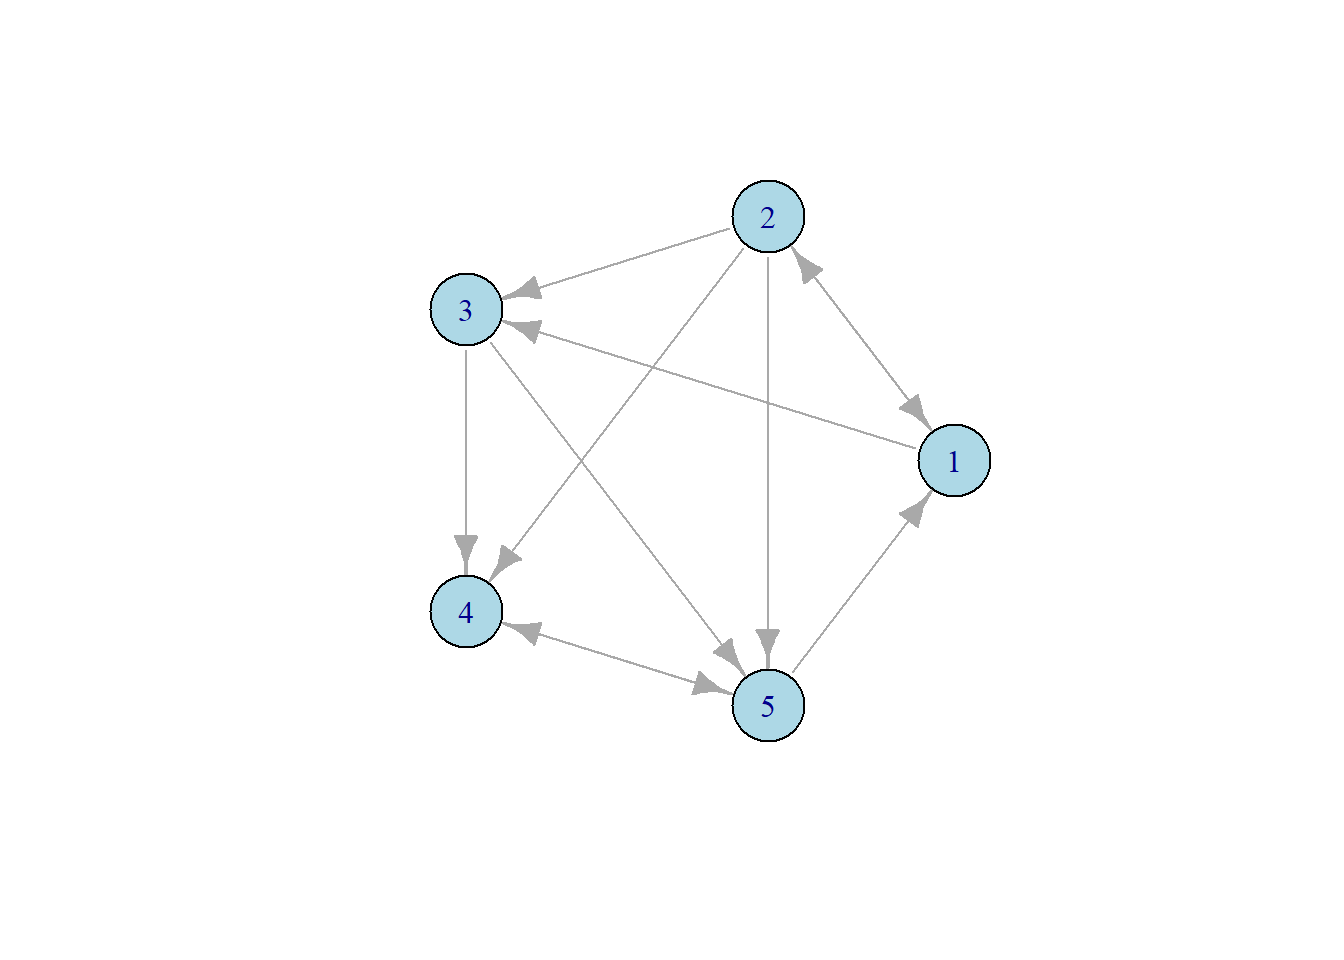
\includegraphics[width=0.75\linewidth]{_main_files/figure-latex/network-1} 

}

\caption{A small network}\label{fig:network}
\end{figure}

A random surfer on Site 1 has two links to choose, Site 2 or Site 3. Suppose they choose randomly; that is, they choose each site with probability 1/2 (Fig. \ref{fig:surfer}).

\begin{figure}

{\centering 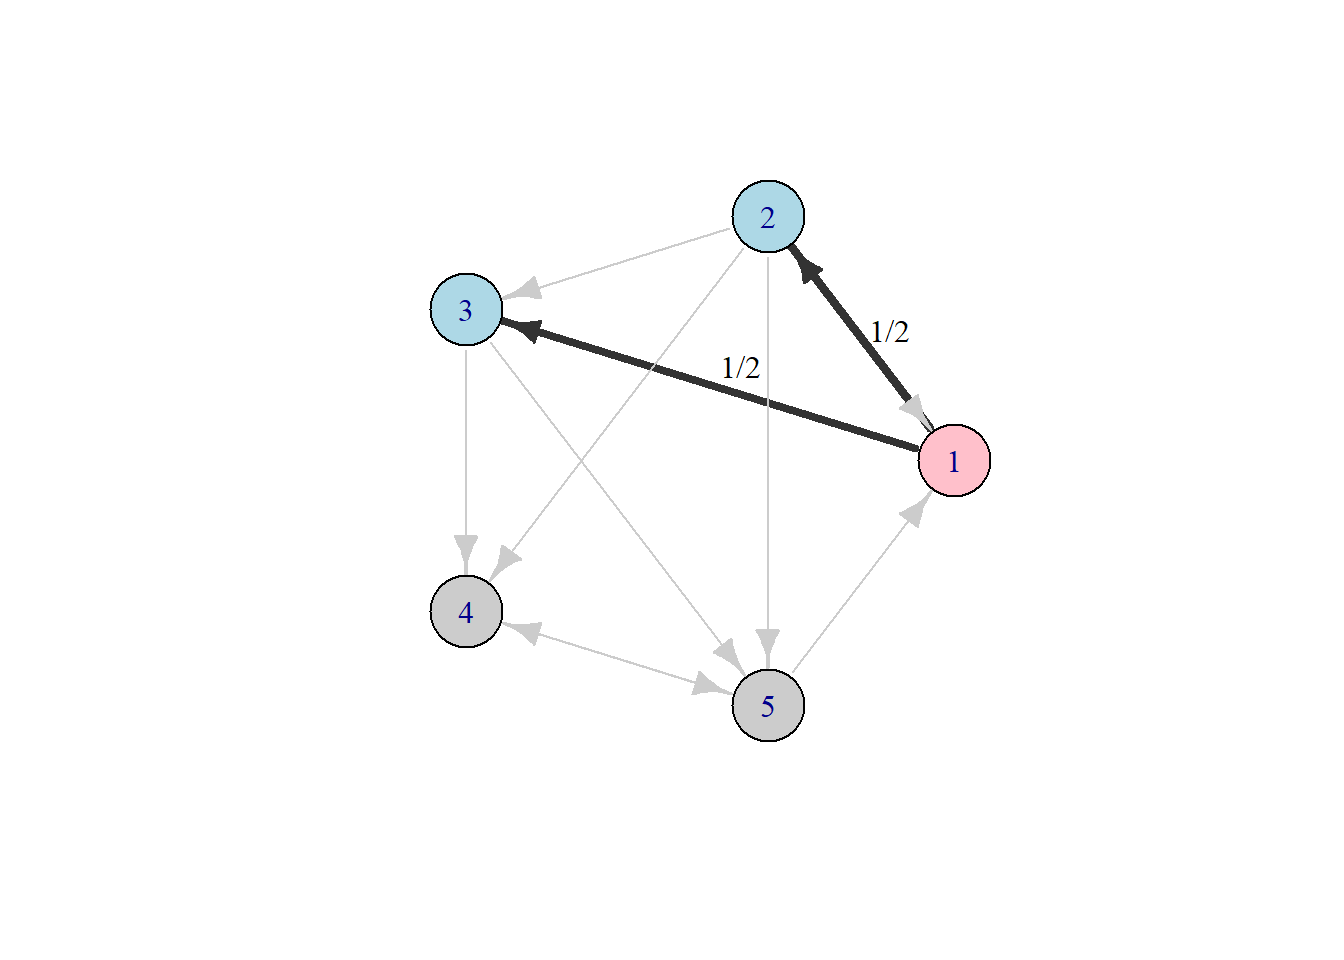
\includegraphics[width=0.75\linewidth]{_main_files/figure-latex/surfer-1} 

}

\caption{A random surfer on the network}\label{fig:surfer}
\end{figure}

A random surfer at Site 2 can go to any of the other four sites, each with probability 1/4 (Fig. \ref{fig:surfer2}).

\begin{figure}

{\centering 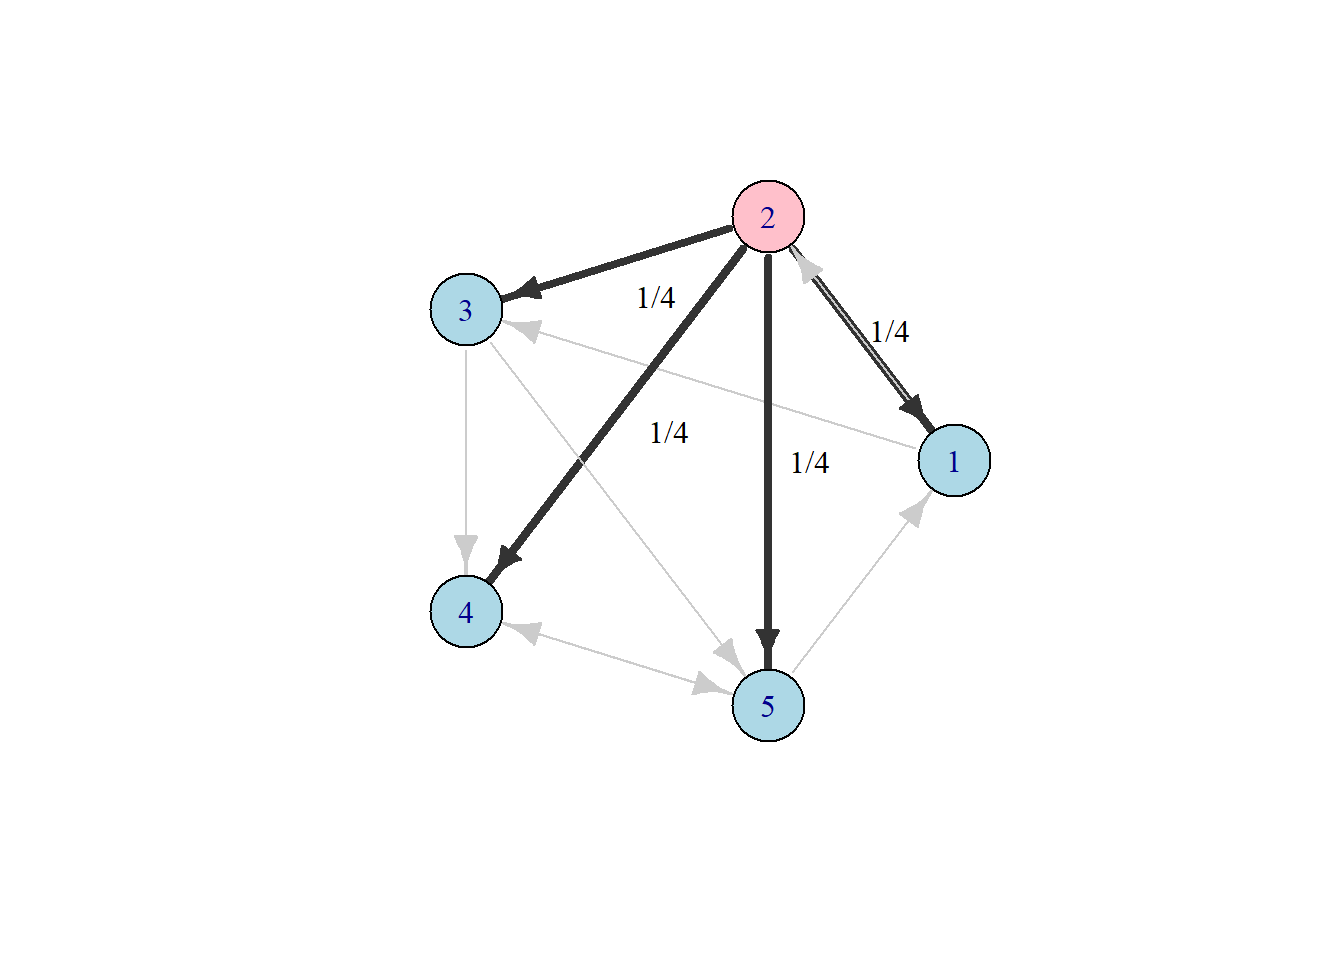
\includegraphics[width=0.75\linewidth]{_main_files/figure-latex/surfer2-1} 

}

\caption{The choices from Site 2}\label{fig:surfer2}
\end{figure}

We can put these probabilities into the columns of a matrix called a \emph{transition matrix}. Sites that aren't linked to get the probability 0 assigned.

\[\mathbf{S}=\begin{bmatrix}0 & 0.25 & 0 & 0 & 0.5\\
0.5 & 0 & 0 & 0 & 0\\
0.5 & 0.25 & 0 & 0 & 0\\
0 & 0.25 & 0.5 & 0 & 0.5\\
0 & 0.25 & 0.5 & 1 & 0\end{bmatrix}
\]

The \(s_{ij}\) entry is the probability of going \emph{to} vertex \(i\) \emph{from} vertex \(j\). For example \(s_{42}=0.25=P(2\to 4)\).

\begin{notebox}
\textbf{Important note:} The row and columns in this transition matrix have the opposite roles from what they had in a directed adjacency matrix. There is a reason for doing it this way that we will get to soon.

\end{notebox}

\subsection*{Stochastic matrices}\label{stochastic-matrices}
\addcontentsline{toc}{subsection}{Stochastic matrices}

The matrix \(\mathbf{S}\) is what we call a (column) stochastic matrix\index{Stochastic matrix}:

\begin{itemize}
\item
  all the entries are between 0 and 1.
\item
  all the columns add up to 1.
\end{itemize}

\begin{notebox}
\textbf{Another important note:} It is somewhat traditional to have the \emph{rows} of a stochastic matrix adding up to 1 (i.e., \emph{row stochastic}). We will soon be using eigenvalues and eigenvectors, and to be consistent with how we use them, we want the columns to add to 1 (\emph{column stochastic}).

\end{notebox}

Powers of stochastic matrices have a property that is similar to a property of adjacency matrices.

\[\mathbf{S}^2=\begin{bmatrix}
   0 & 0.25 & 0 & 0 & 0.5\\
0.5 & 0 & 0 & 0 & 0\\
0.5 & 0.25 & 0 & 0 & 0\\
\mathbf{0} & \mathbf{0.25} & \mathbf{0.5} & \mathbf{0} & \mathbf{0.5}\\
0 & 0.25 & 0.5 & 1 & 0 \end{bmatrix}
\begin{bmatrix}
   0 & \mathbf{0.25} & 0 & 0 & 0.5\\
0.5 & \mathbf{0} & 0 & 0 & 0\\
0.5 & \mathbf{0.25} & 0 & 0 & 0\\
0 & \mathbf{0.25} & 0.5 & 0 & 0.5\\
0 & \mathbf{0.25} & 0.5 & 1 & 0 
\end{bmatrix}\]

The product of the fourth row of \(\mathbf{S}\) and the second column of \(\mathbf{S}\) is

\[0\cdot 0.25+0.25\cdot 0+\underbrace{0.5\cdot 0.25}_{P(3\to 4)P(2\to 3)}+0\cdot 0.25+0.5\cdot0.25= 0.25\]

The highlighted product is the probability of going from Site 2 to Site 3 and then from Site 3 to Site 4. The sum is the probability of going from Site 2 to Site 4 in two clicks, the \(\mathbf{S}^2_{42}\) entry.

The columns of \(\mathbf{S}^2\) give the probabilities of going from one site to another in exactly two clicks. The columns of \(\mathbf{S}^r\) will give the probabilities of going from one site to another in exactly \(r\) clicks. In our example,

\[\mathbf{S}^2=\begin{bmatrix}0.125 & 0.125 & 0.25 & 0.5 & 0\\
0 & 0.125 & 0 & 0 & 0.25\\
0.125 & 0.125 & 0 & 0 & 0.25\\
0.375 & 0.25 & 0.25 & 0.5 & 0\\
0.375 & 0.375 & 0.5 & 0 & 0.5\end{bmatrix}.\]

As an example, the probability of going from Site 2 to Site 5 in two clicks is 0.375. You can't go from Site 3 to Site 2 in two clicks. You can only get to Sites 1, 4, or 5 (Column 3). Note that \(\mathbf{S}^2\) is also column stochastic, as every positive integer power of \(\mathbf{S}\) will be. That is a consequence of the following theorem.

\begin{theorembox}

\begin{theorem}
Let \(\mathbf{S}\) and \(\mathbf{T}\) be two \(n\times n\) column stochastic matrices. Then the product \(\mathbf{ST}\) is also column stochastic.
\end{theorem}

\end{theorembox}

\begin{proof}
First note that, since all the entries in \(\mathbf{S}\) and \(\mathbf{T}\) are nonnegative, the entries in \(\mathbf{ST}\) will also be nonnegative.

Let \(\mathbf{v}\) be the \(n\)-dimensional row vector \(\begin{bmatrix} 1 & 1 & \cdots & 1\end{bmatrix}\) and let \(\mathbf{a}=\begin{bmatrix} a_1\\a_2\\ \vdots \\ a_n\end{bmatrix}\) be an \(n\)-dimensional column vector. Then \(\mathbf{v}\mathbf{a}=1\cdot a_1+1\cdot a_2+\cdots+1\cdot a_n=a_1+a_2+\cdots a_n\). That is, multiplication on the left by \(\mathbf{v}\) sums the entries in that vector. Now note that the product

\begin{align*}
\mathbf{v}\mathbf{S}&=\mathbf{v}\begin{bmatrix}\mathbf{s}_1 & \mathbf{s}_2 & \cdots & \mathbf{s}_n\end{bmatrix}\\
&=\begin{bmatrix}\mathbf{v}\mathbf{s}_1 & \mathbf{v}\mathbf{s}_2 & \cdots & \mathbf{v}\mathbf{s}_n\end{bmatrix}\\
&=\begin{bmatrix} 1 & 1 & \cdots & 1\end{bmatrix},
\end{align*}

since all of the \(\mathbf{s}_i\) have entries that sum to 1. The product \(\mathbf{v}(\mathbf{ST})\) will be a row vector consisting of the column sums of \(\mathbf{ST}\). And

\[\mathbf{v}(\mathbf{ST})=(\mathbf{v}\mathbf{S})\mathbf{T}=\begin{bmatrix} 1 & 1 & \cdots & 1\end{bmatrix}\mathbf{T}=\begin{bmatrix} 1 & 1 & \cdots & 1\end{bmatrix},\]

because the columns of \(\mathbf{T}\) also sum to 1. Since \(\mathbf{ST}\) is a matrix with nonnegative entries whose columns sum to 1, it is column stochastic.
\end{proof}

Now let's consider what happens when we unleash an army of surfers on the network. Let's start with them evenly spread out among the sites. They can be represented by the vector

\[\mathbf{v}=\begin{bmatrix}0.2\\0.2\\0.2\\0.2\\0.2\end{bmatrix}.\]

If the surfers all click at the same time, their distribution after that click is given by

\[\mathbf{S}\mathbf{v}=\begin{bmatrix}0 & 0.25 & 0 & 0 & 0.5\\
0.5 & 0 & 0 & 0 & 0\\
0.5 & 0.25 & 0 & 0 & 0\\
0 & 0.25 & 0.5 & 0 & 0.5\\
0 & 0.25 & 0.5 & 1 & 0\end{bmatrix}\begin{bmatrix}0.2\\0.2\\0.2\\0.2\\0.2\end{bmatrix}=\begin{bmatrix} 0.15 \\ 0.10 \\ 0.15 \\ 0.25 \\ 0.35\end{bmatrix}.\]

After two and three clicks, the distributions are

\[\mathbf{S}(\mathbf{S}\mathbf{v})=\mathbf{S}^2\mathbf{v}=\begin{bmatrix}0.2\\0.075\\0.1\\0.275\\0.35\end{bmatrix} \text{ and } \mathbf{S}^3\mathbf{v}=\begin{bmatrix}0.19375\\0.1\\0.11875\\0.24375\\0.34375\end{bmatrix}.\]

What happens in the long run? After a few more clicks, the distribution appears to stabilize (Fig. \ref{fig:rwalker}).

\begin{figure}

{\centering 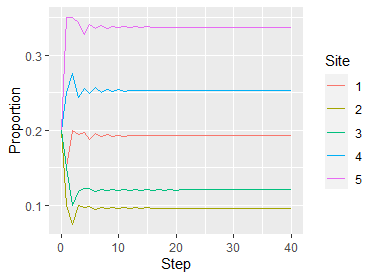
\includegraphics[width=0.75\linewidth]{images/rw4} 

}

\caption{Distribution of random surfers as a function of the number of steps}\label{fig:rwalker}
\end{figure}

After a lot of clicks, we have

\[\mathbf{S}^{57}\mathbf{v}=(0.19277,0.09638,0.12048,0.25301,0.33735)\]

and

\[\mathbf{S}^{58}\mathbf{v}=\mathbf{S}(\mathbf{S}^{57}\mathbf{v})=(0.19277,0.09638,0.12048,0.25301,0.33735)\]

Some notes:

\begin{itemize}
\item
  We can use these values to rank our websites. Site 5 seems to be the most popular, followed by Sites 4,1,3, and 2.
\item
  This stable distribution is going to be an eigenvector for \(\mathbf{S}\), with a corresponding eigenvalue of 1!
\end{itemize}

It turns out that a stochastic matrix will always have the value 1 as an eigenvalue. It is actually the dominant (largest in absolute value) eigenvalue. And when we scale the corresponding eigenvector so that the terms add up to 1, we get our stable distribution! (Remember a similar phenomenon with the Leslie matrix?)

So, this seems to be a good method for ranking websites based on links in and out. But there are a few problems that can come up.

\textbf{Issue 1: dangling nodes}

A \emph{dangling node}\index{Dangling node} on a graph is a vertex that has no edges leaving it. In this graph (Fig. \ref{fig:dangling}), vertex 5 is dangling, and the corresponding column in the transition matrix has all 0s. It is \emph{substochastic}\index{Substochastic matrix}. The surfers have nowhere to go.

\begin{figure}

{\centering 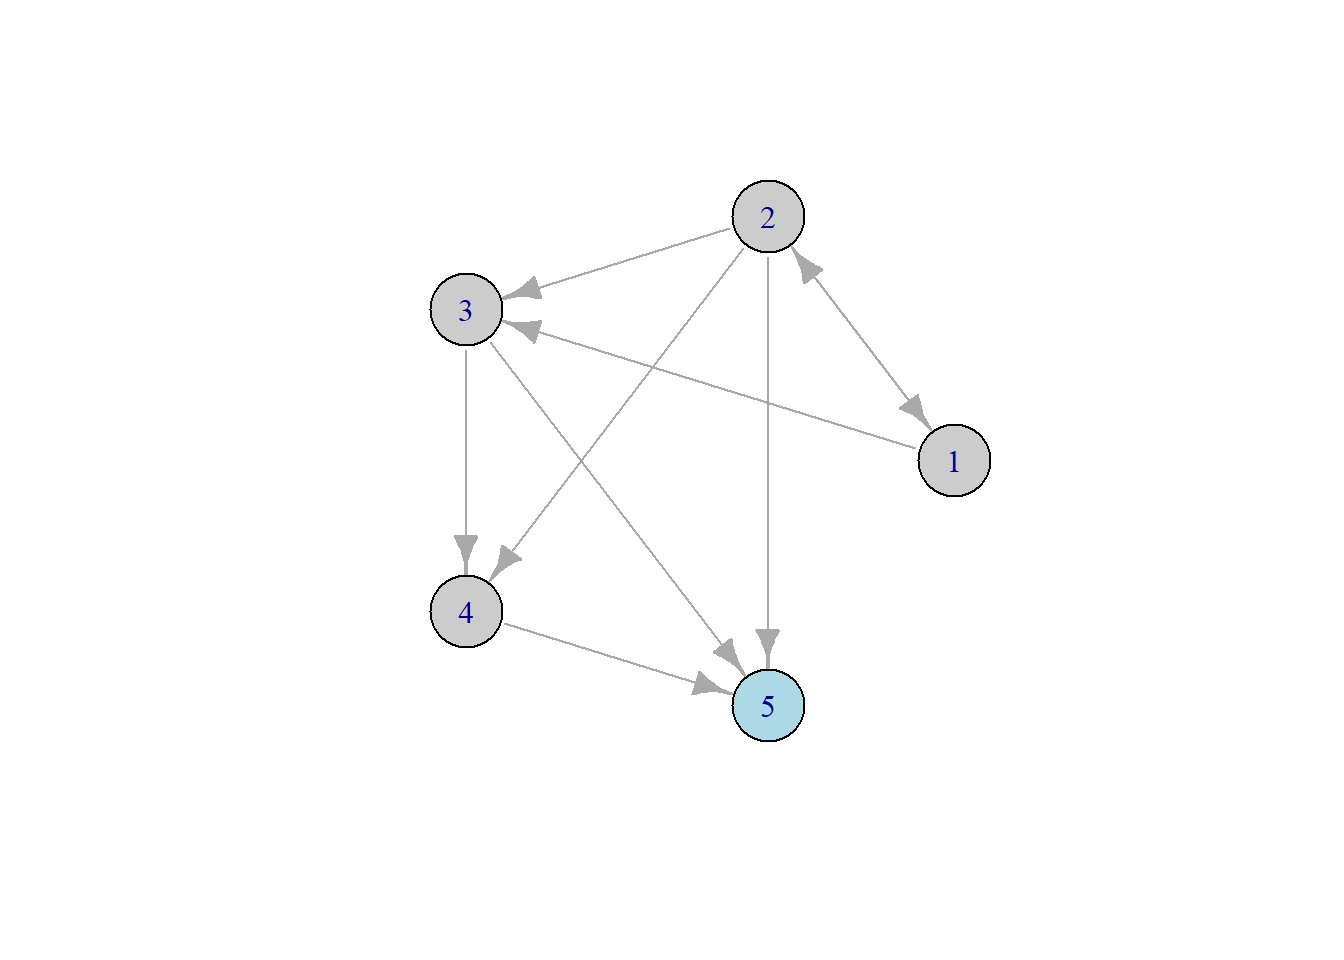
\includegraphics[width=0.75\linewidth]{_main_files/figure-latex/dangling-1} 

}

\caption{A dangling node}\label{fig:dangling}
\end{figure}

Here is the transition matrix for the graph.

\[\mathbf{S}=\begin{bmatrix} 0 & 0.25 & 0 & 0 & 0\\
0.5 & 0 & 0 & 0 & 0\\
0.5 & 0.25 & 0 & 0 & 0\\
0 & 0.25 & 0.5 & 0 & 0\\0 & 0.25 & 0.5 & 1 & 0\end{bmatrix}\]

Adding a loop at vertex 5 would cause all the traffic to get stuck there, leading to a stable distribution of \((0,0,0,0,1)\), which is not particularly useful for ratings.

\textbf{Issue 2: Disconnected graphs}

It is also possible that the graph consists of two or more distinct groups\index{Disconnected graph} that have no connections between them, as in Figure \ref{fig:disconnected}.

\begin{figure}

{\centering 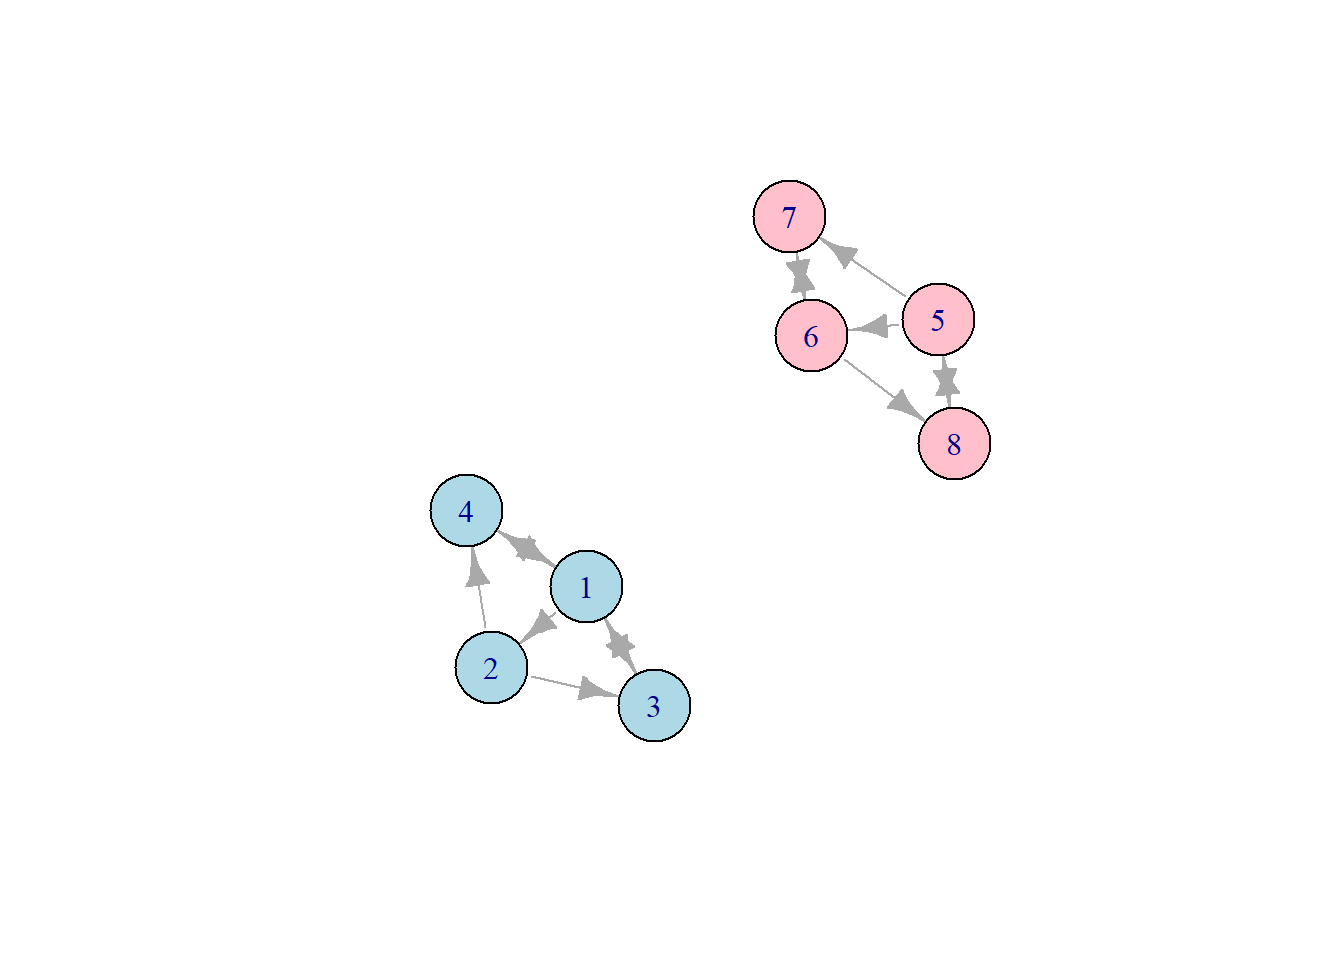
\includegraphics[width=0.75\linewidth]{_main_files/figure-latex/disconnected-1} 

}

\caption{A disconnected graph}\label{fig:disconnected}
\end{figure}

In this case, \(\lambda=1\) will actually be a double eigenvalue, and there won't be a unique stable solution.

\textbf{Issue 3: Cycling}

A third problem that comes up is the rock/paper/scissors issue. If a graph contains a cycle\index{Cycle! in a graph} that can't be exited, as in Figure \ref{fig:cycle}, there can be a stable solution, but it might not be achieved in any iteration process. Note: the cycle could be of any length greater than 1.

\begin{figure}

{\centering 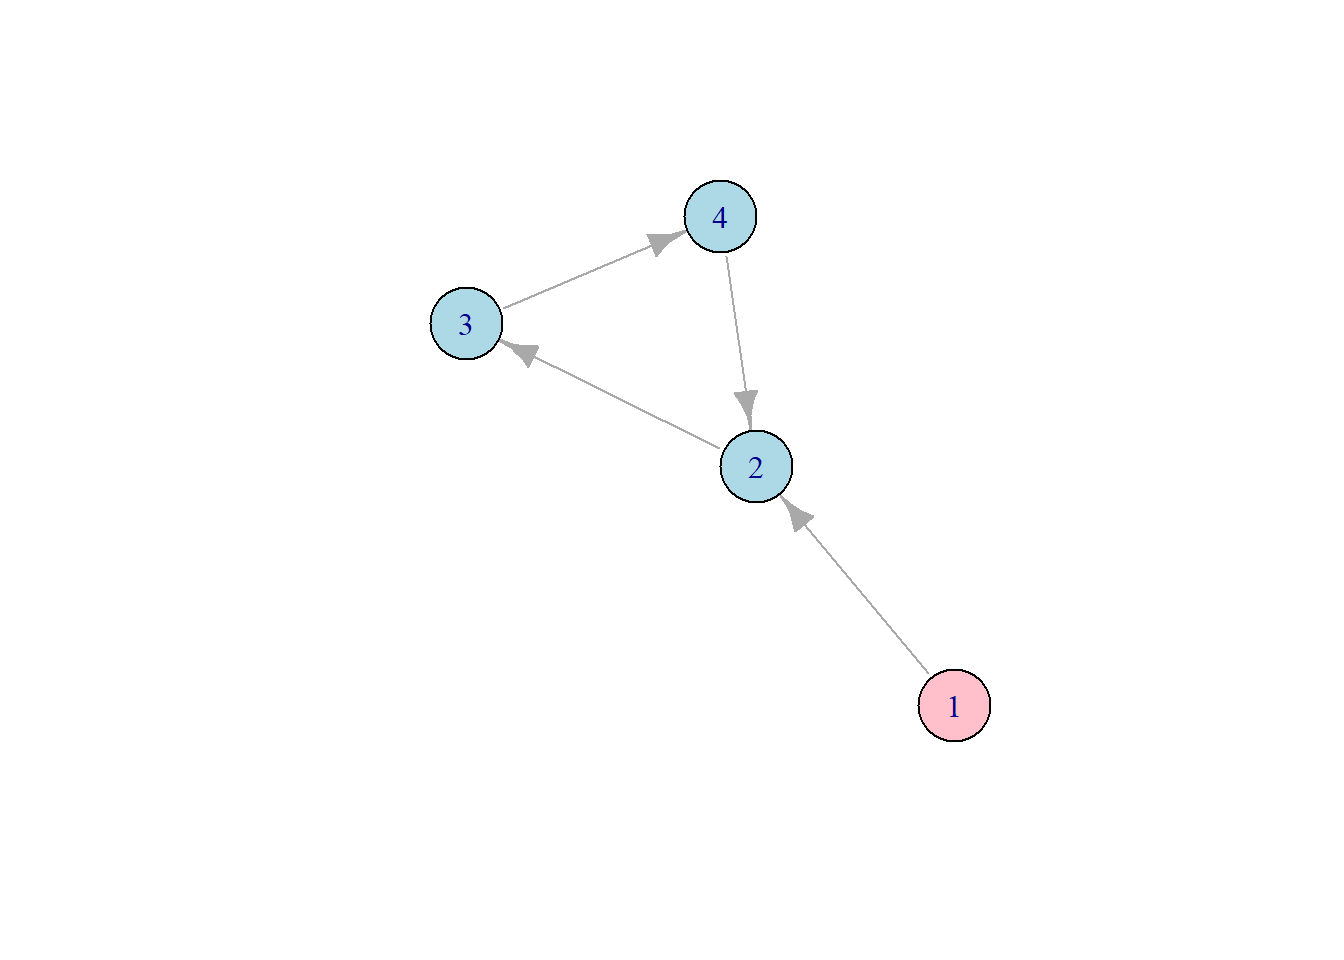
\includegraphics[width=0.75\linewidth]{_main_files/figure-latex/cycle-1} 

}

\caption{a cycle}\label{fig:cycle}
\end{figure}

There are some conditions on the stochastic matrix and underlying graph that will lead to a unique stable solution. For that, we need some definitions.

\begin{defbox}

\begin{definition}

Let \(\mathbf{A}\) be an \(n\times n\) matrix.

\begin{itemize}
\item
  \(\mathbf{A}\) is \textbf{nonnegative}\index{Nonnegative matrix} (\(\mathbf{A}\geq 0\)) if all entries in \(\mathbf{A}\) are nonnegative.
\item
  \(\mathbf{A}\) is \textbf{positive}\index{Positive matrix} (\(\mathbf{A}>0\)) if all entries in \(\mathbf{A}\) are positive.
\item
  \(\mathbf{A}\) is \textbf{regular}\index{Regular matrix} if \(\mathbf{A}\geq 0\) and there exists a positive integer \(k\) such that \(\mathbf{A}^k\) is a positive matrix.
\end{itemize}

\end{definition}

\end{defbox}

Note that stochastic matrices are nonnegative. For a graph and its transition matrix, \emph{regular} means that for some \(k\) it is possible to get from every vertex to every other vertex in exactly \(k\) steps.

The Perron-Frobenius Theorem\index{Perron-Frobenius Theorem} is key for graph-based ranking methods\autocite{No1}.

\begin{theorembox}

\begin{theorem}[The Perron-Frobenius Theorem for Stochastic Matrices]

Let \(\mathbf{A}\) be a regular stochastic matrix. Then

\begin{enumerate}
\def\labelenumi{\arabic{enumi}.}
\item
  The matrix \(\mathbf{A}\) has \(\lambda_1=1\) as an eigenvalue of multiplicty \(1.\) The eigenvector \(\mathbf{v}_1\) corresponding to \(\lambda_1\) can be chosen so that it has all positive entries that sum to \(1\) (a positive \textbf{probability vector}\index{Probability vector}).
\item
  All other eigenvalues \(\lambda_j\) have \(|\lambda_j|<1\). The corresponding eigenvectors have entries that sum to \(0.\)
\item
  If \(\mathbf{p}\) is any probability vector, then \(\mathbf{A}^n\mathbf{p}\to\mathbf{v}_1\) as \(n\to\infty\). In particular, the columns of \(\mathbf{A}^n\) are all approaching \(\mathbf{v}_1\).
\end{enumerate}

\end{theorem}

\end{theorembox}

The stochastic version of the Perron-Frobenius Theorem is a special case of a more general theorem \autocite{Meyer}.

\subsection*{Markov Chains}\label{markov-chains}
\addcontentsline{toc}{subsection}{Markov Chains}

The graph/transition matrix pair is an example of a \emph{Markov chain}\index{Markov chain}. A Markov chain is a collection of \emph{states} (for us, the vertices in a graph) with associated probabilities of moving from one state to another. The probabilities for moving from one state to another only depend on the current state and not on any past state or sequence of states.

In addition to the application we've already seen, Markov chains can be used to simulate things such as baseball games or to create simple weather models. Here is an example of one of them.

Suppose there are three kinds of days: sunny, cloudy, and rainy. The transition matrix from one type of day to another might look like this.

\begin{examplebox}

\begin{example}
\leavevmode

\begin{longtable}[]{@{}lllll@{}}
\toprule\noalign{}
& & & \textbf{Today} & \\
\midrule\noalign{}
\endhead
\bottomrule\noalign{}
\endlastfoot
& & Sunny & Cloudy & Rainy \\
& Sunny & 0.7 & 0.5 & 0.4 \\
\textbf{Tomorrow} & Cloudy & 0.2 & 0.3 & 0.5 \\
& Rainy & 0.1 & 0.2 & 0.1 \\
\end{longtable}

If we square the transition matrix, we get the probabilities for two days out.

\[
\mathbf{S}^2=\begin{bmatrix}
    0.63 & 0.58 & 0.57 \\
    0.25 & 0.29 & 0.28\\
    0.12 & 0.13 & 0.15
    \end{bmatrix}
\]

If it's sunny today, there's a 63\% chance that it will be sunny in two days. If it's cloudy today, there's a 13\% chance that it will be rainy in two days. What will happen in the long run? Since this weather forecaster is a positive stochastic matrix, when we raise it to higher and higher powers, all three columns will approach the stable distribution.

\[
\textbf{S}^{100}=\begin{bmatrix}
    0.6091954 & 0.6091954 & 0.6091954 \\
    0.2643678 & 0.2643678  & 0.2643678\\
    0.1264368 & 0.1264368 & 0.1264368 
    \end{bmatrix}
\]

If you think about it, what this is saying is that the weather today won't tell us much about the weather 100 days from today (ignoring seasons and all that). About 61\% of the days will be sunny, 26\% will be cloudy, and 13\% will be rainy.

\end{example}

\end{examplebox}

\subsection*{Why is 1 always an eigenvalue?}\label{why-is-1-always-an-eigenvalue}
\addcontentsline{toc}{subsection}{Why is 1 always an eigenvalue?}

We close this section by taking care of some unfinished business. The Perron-Frobenius Theorem guarantees us that a stochastic matrix will have an eigenvalue of 1, but there is an easier way to see that.

We've already observed that

\[\begin{bmatrix} 1 & 1 & \cdots & 1\end{bmatrix}\mathbf{S}=\begin{bmatrix} 1 & 1 & \cdots & 1\end{bmatrix}\]

for a stochastic matrix \(\mathbf{S}\) and the appropriately sized row vector of ones. That means that

\[(\begin{bmatrix} 1 & 1 & \cdots & 1\end{bmatrix}\mathbf{S})^T=\begin{bmatrix}1\\1\\ \vdots \\ 1\end{bmatrix}\]

or

\[\mathbf{S}^T\begin{bmatrix}1\\1\\ \vdots \\ 1\end{bmatrix}=\begin{bmatrix}1\\1\\ \vdots \\ 1\end{bmatrix}.\]

In other words, the column vector of ones is an eigenvector for \(\mathbf{S}^T\) with corresponding eigenvalue 1. Since matrices and their transposes share the same eigenvalues, 1 is also an eigenvalue for \(S\).

\section{The Markov and Oracle Ranking Methods}\label{the-markov-and-oracle-ranking-methods}

There are several Markov chain-based ranking methods. We will see two in this section. The \emph{Markov method}\index{Markov method}, which is modeled on the PageRank algorithm \autocite{PageRank}, was developed by Amy N. Langville and Carl D. Meyer \autocite{No1}. The Oracle method\index{Oracle method} was developed by E. Cabral Balreira, Brian Miceli, and T. Tegtmeyer \autocite{Oracle}.

\subsection*{The Markov method}\label{the-markov-method}
\addcontentsline{toc}{subsection}{The Markov method}

The key step in any Markov chain-based method is to create a regular matrix, so that we can take advantage of the Perron-Frobenious theorem. Recall the graph we saw in Figure \ref{fig:dangling}. The corresponding transition matrix is here

\[\mathbf{T}=\begin{bmatrix} 0 & 0.25 & 0 & 0 & 0\\
0.5 & 0 & 0 & 0 & 0\\
0.5 & 0.25 & 0 & 0 & 0\\
0 & 0.25 & 0.5 & 0 & 0\\0 & 0.25 & 0.5 & 1 & 0\end{bmatrix}.\]

The first step is to replace the column of all zeros with a column whose entries are all \(1/n\), where \(n\) is the number of vertices or teams.

\[\mathbf{T}=\begin{bmatrix} 0 & 0.25 & 0 & 0 & 0\\
0.5 & 0 & 0 & 0 & 0\\
0.5 & 0.25 & 0 & 0 & 0\\
0 & 0.25 & 0.5 & 0 & 0\\0 & 0.25 & 0.5 & 1 & 0\end{bmatrix}\to \mathbf{S}=\begin{bmatrix} 0 & 0.25 & 0 & 0 & 0.2\\
0.5 & 0 & 0 & 0 & 0.2\\
0.5 & 0.25 & 0 & 0 & 0.2\\
0 & 0.25 & 0.5 & 0 & 0.2\\0 & 0.25 & 0.5 & 1 & 0.2\end{bmatrix}\]

This is like replacing a site with no outgoing links with one that links to all of the other sites, including itself. We still need to do something to ensure regularity of the transition matrix. The Langville-Meyer/PageRank solution is brutally simple. It introduces a \emph{teleportation matrix}\index{Teleportation matrix}. A certain fraction of the time, say \(\alpha\), the random surfers will follow the original network. The remainder of the time, the surfers will magically teleport to any other site in the network, with equal probability. The \(n\times n\) teleportation matrix looks like this:

\[\mathbf{E}=\begin{bmatrix} 1/n & 1/n & \cdots & 1/n\\
1/n & 1/n & \cdots & 1/n\\
\vdots & \vdots & \ddots & \vdots \\
1/n & 1/n & \cdots & 1/n \end{bmatrix}.\]

When we combine the transition matrix and the teleportation matrix, we get a new stochastic matrix

\[\textbf{G}=\alpha \textbf{S}\textbf{}+(1-\alpha)\textbf{E}\]

that is regular (indeed, positive) by design. The probability eigenvector corresponding to the eigenvalue 1 will be our ratings vector. We can experiment with the value of \(\alpha\), but \(\alpha = 0.85\) is a common value. For our dangling node example,

\begin{align*}
\mathbf{G}&=0.85\begin{bmatrix} 0 & 0.25 & 0 & 0 & 0.2\\
0.5 & 0 & 0 & 0 & 0.2\\
0.5 & 0.25 & 0 & 0 & 0.2\\
0 & 0.25 & 0.5 & 0 & 0.2\\0 & 0.25 & 0.5 & 1 & 0.2\end{bmatrix}+0.15\begin{bmatrix} 0.2 & 0.2 & 0.2 & 0.2 & 0.2\\
0.2 & 0.2 & 0.2 & 0.2 & 0.2\\
0.2 & 0.2 & 0.2 & 0.2 & 0.2\\
0.2 & 0.2 & 0.2 & 0.2 & 0.2\\
0.2 & 0.2 & 0.2 & 0.2 & 0.2 \end{bmatrix}\\
&=\begin{bmatrix}
0.03 & 0.2425 & 0.03 & 0.03 & 0.2\\
0.455 & 0.03 & 0.03 & 0.03 & 0.2\\
0.455 & 0.2425 & 0.03 & 0.03 & 0.2\\
0.03 & 0.2425 & 0.455 & 0.03 & 0.2\\
0.03 & 0.2425 & 0.455 & 0.88 & 0.2
\end{bmatrix}.
\end{align*}

The ratings eigenvector is

\[\mathbf{v}=(0.1223049, 0.1437397, 0.1742844, 0.1963758, 0.3632952).\]

\begin{examplebox}

\begin{example}

Here is one way to implement the Markov method in R, demonstrated on our toy example.

\begin{Shaded}
\begin{Highlighting}[]
\FunctionTok{library}\NormalTok{(igraph)}
\FunctionTok{library}\NormalTok{(expm)}
\NormalTok{teams }\OtherTok{\textless{}{-}} \FunctionTok{c}\NormalTok{(}\StringTok{"Aardvarks"}\NormalTok{, }\StringTok{"Beagles"}\NormalTok{, }\StringTok{"Crocs"}\NormalTok{,  }
          \StringTok{"Donkeys"}\NormalTok{, }\StringTok{"Egrets"}\NormalTok{)}
\NormalTok{results }\OtherTok{\textless{}{-}}\FunctionTok{c}\NormalTok{ (}\DecValTok{1}\NormalTok{,}\DecValTok{2}\NormalTok{,}\DecValTok{1}\NormalTok{,}\DecValTok{3}\NormalTok{,}\DecValTok{5}\NormalTok{,}\DecValTok{1}\NormalTok{,}\DecValTok{2}\NormalTok{,}\DecValTok{3}\NormalTok{,}\DecValTok{2}\NormalTok{,}\DecValTok{4}\NormalTok{,}\DecValTok{4}\NormalTok{,}\DecValTok{3}\NormalTok{,}\DecValTok{5}\NormalTok{,}\DecValTok{3}\NormalTok{,}\DecValTok{5}\NormalTok{,}\DecValTok{4}\NormalTok{)}
\NormalTok{gtoy }\OtherTok{\textless{}{-}} \FunctionTok{graph}\NormalTok{(results)}
\NormalTok{coords }\OtherTok{\textless{}{-}} \FunctionTok{layout\_in\_circle}\NormalTok{(gtoy)}
\FunctionTok{plot}\NormalTok{(gtoy, }\AttributeTok{vertex.label =}\NormalTok{ teams, }\AttributeTok{vertex.size =} \DecValTok{50}\NormalTok{,  }
     \AttributeTok{vertex.color =} \StringTok{"lightblue"}\NormalTok{, }\AttributeTok{layout =}\NormalTok{ coords)}
\end{Highlighting}
\end{Shaded}

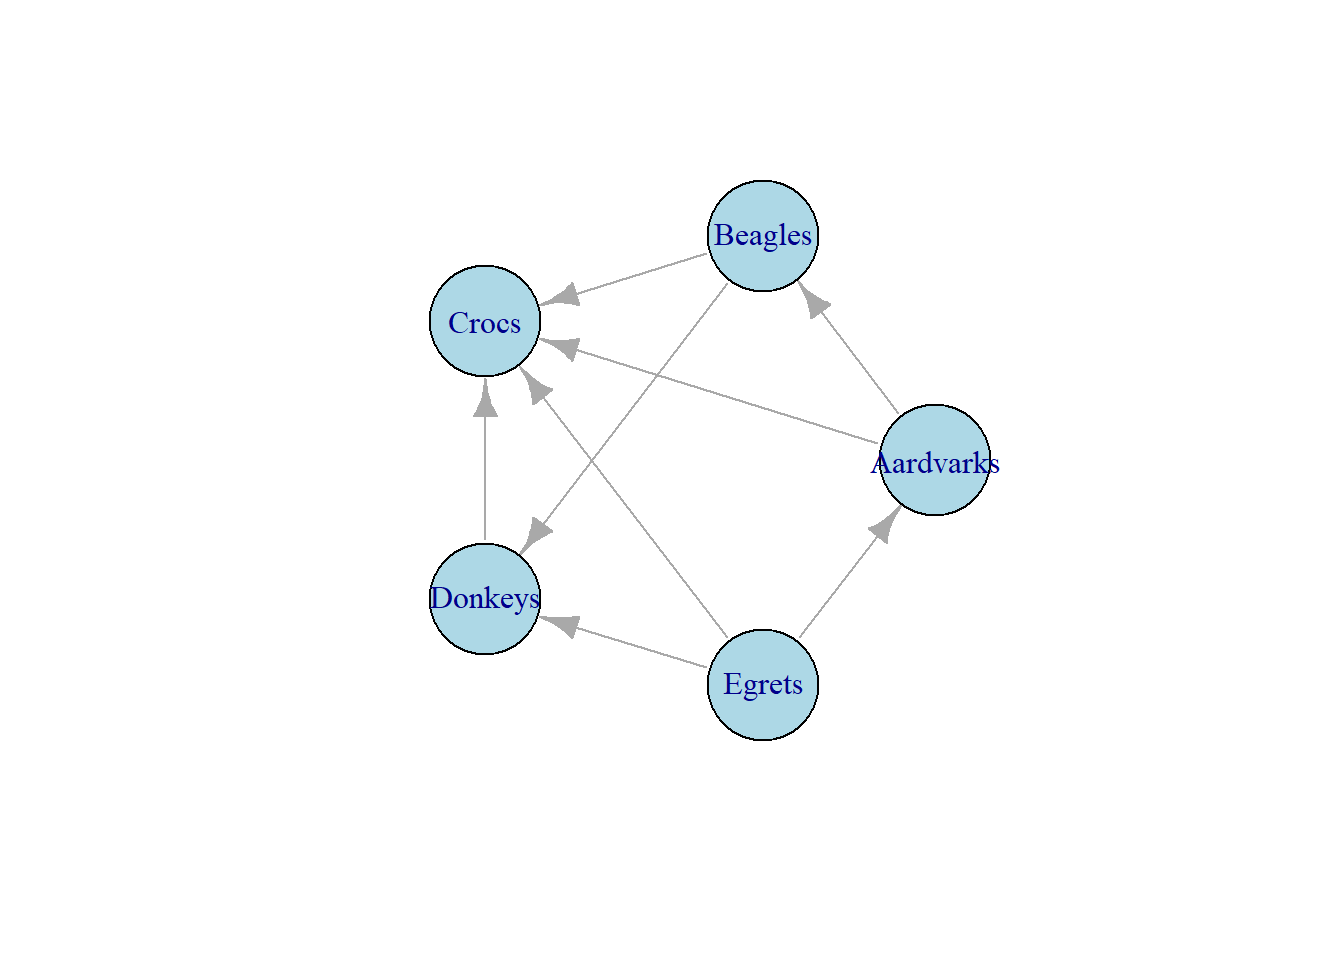
\includegraphics{_main_files/figure-latex/markov-1.pdf}

\begin{Shaded}
\begin{Highlighting}[]
\CommentTok{\# We take the transpose of the adjacency matrix}
\NormalTok{T }\OtherTok{\textless{}{-}} \FunctionTok{t}\NormalTok{(}\FunctionTok{as.matrix}\NormalTok{(}\FunctionTok{as\_adjacency\_matrix}\NormalTok{(gtoy))) }
\NormalTok{T}
\end{Highlighting}
\end{Shaded}

\begin{verbatim}
##      [,1] [,2] [,3] [,4] [,5]
## [1,]    0    0    0    0    1
## [2,]    1    0    0    0    0
## [3,]    1    1    0    1    1
## [4,]    0    1    0    0    1
## [5,]    0    0    0    0    0
\end{verbatim}

\begin{Shaded}
\begin{Highlighting}[]
\NormalTok{s }\OtherTok{\textless{}{-}} \FunctionTok{nrow}\NormalTok{(T)}
\CommentTok{\# Next, we identify the dangling nodes, replace their}
\CommentTok{\# columns with ones, and then make the transition }
\CommentTok{\# matrix by scaling the column sums.}

\NormalTok{D }\OtherTok{\textless{}{-}} \FunctionTok{colSums}\NormalTok{(T)}
\NormalTok{dangling }\OtherTok{\textless{}{-}} \FunctionTok{which}\NormalTok{(D }\SpecialCharTok{==} \DecValTok{0}\NormalTok{)}
\NormalTok{T[, dangling] }\OtherTok{\textless{}{-}} \DecValTok{1}
\NormalTok{T}
\end{Highlighting}
\end{Shaded}

\begin{verbatim}
##      [,1] [,2] [,3] [,4] [,5]
## [1,]    0    0    1    0    1
## [2,]    1    0    1    0    0
## [3,]    1    1    1    1    1
## [4,]    0    1    1    0    1
## [5,]    0    0    1    0    0
\end{verbatim}

\begin{Shaded}
\begin{Highlighting}[]
\NormalTok{scale }\OtherTok{\textless{}{-}} \FunctionTok{diag}\NormalTok{(}\DecValTok{1}\SpecialCharTok{/}\FunctionTok{colSums}\NormalTok{(T))}
\NormalTok{S }\OtherTok{\textless{}{-}}\NormalTok{ T}\SpecialCharTok{\%*\%}\NormalTok{scale }\CommentTok{\#multiplication on right acts on the columns}
\NormalTok{S}
\end{Highlighting}
\end{Shaded}

\begin{verbatim}
##      [,1] [,2] [,3] [,4]      [,5]
## [1,]  0.0  0.0  0.2    0 0.3333333
## [2,]  0.5  0.0  0.2    0 0.0000000
## [3,]  0.5  0.5  0.2    1 0.3333333
## [4,]  0.0  0.5  0.2    0 0.3333333
## [5,]  0.0  0.0  0.2    0 0.0000000
\end{verbatim}

\begin{Shaded}
\begin{Highlighting}[]
\CommentTok{\# Now we add the teleportation matrix to get the G matrix}
\NormalTok{G }\OtherTok{\textless{}{-}} \FloatTok{0.85}\SpecialCharTok{*}\NormalTok{S }\SpecialCharTok{+} \FloatTok{0.15}\SpecialCharTok{*}\FunctionTok{matrix}\NormalTok{(}\DecValTok{1}\SpecialCharTok{/}\NormalTok{s, }\AttributeTok{nrow =}\NormalTok{ s, }\AttributeTok{ncol =}\NormalTok{ s) }
\NormalTok{G}
\end{Highlighting}
\end{Shaded}

\begin{verbatim}
##       [,1]  [,2] [,3] [,4]      [,5]
## [1,] 0.030 0.030  0.2 0.03 0.3133333
## [2,] 0.455 0.030  0.2 0.03 0.0300000
## [3,] 0.455 0.455  0.2 0.88 0.3133333
## [4,] 0.030 0.455  0.2 0.03 0.3133333
## [5,] 0.030 0.030  0.2 0.03 0.0300000
\end{verbatim}

\begin{Shaded}
\begin{Highlighting}[]
\CommentTok{\# Now we raise G to a high power and extract our ratings}
\CommentTok{\# vector}
\NormalTok{(G}\SpecialCharTok{\%\^{}\%}\DecValTok{50}\NormalTok{)[, }\DecValTok{1}\NormalTok{]}
\end{Highlighting}
\end{Shaded}

\begin{verbatim}
## [1] 0.1295831 0.1560467 0.4174933 0.1959030 0.1009739
\end{verbatim}

Here are the ratings. They are presented with the Colley ratings for comparison. Recall that the Colley ratings are not designed to add up to 1. The rankings are the same.

\begin{longtable}[]{@{}lllll@{}}
\toprule\noalign{}
\textbf{Team} & W-L & PCT & Colley Rating & Markov Rating \\
\midrule\noalign{}
\endhead
\bottomrule\noalign{}
\endlastfoot
\textbf{Crocs} & 4-0 & 1.000 & 0.786 & 0.4175 \\
\textbf{Donkeys} & 2-1 & 0.667 & 0.600 & 0.1959 \\
\textbf{Beagles} & 1-2 & 0.333 & 0.457 & 0.1560 \\
\textbf{Aardvarks} & 1-2 & 0.333 & 0.400 & 0.1296 \\
\textbf{Egrets} & 0-3 & 0.000 & 0.257 & 0.1010 \\
\end{longtable}

\end{example}

\end{examplebox}

\subsection*{The Oracle method}\label{the-oracle-method}
\addcontentsline{toc}{subsection}{The Oracle method}

The Oracle method\index{Oracle method} takes a different approach to induce regularity in the transition matrix.

\begin{figure}
\centering
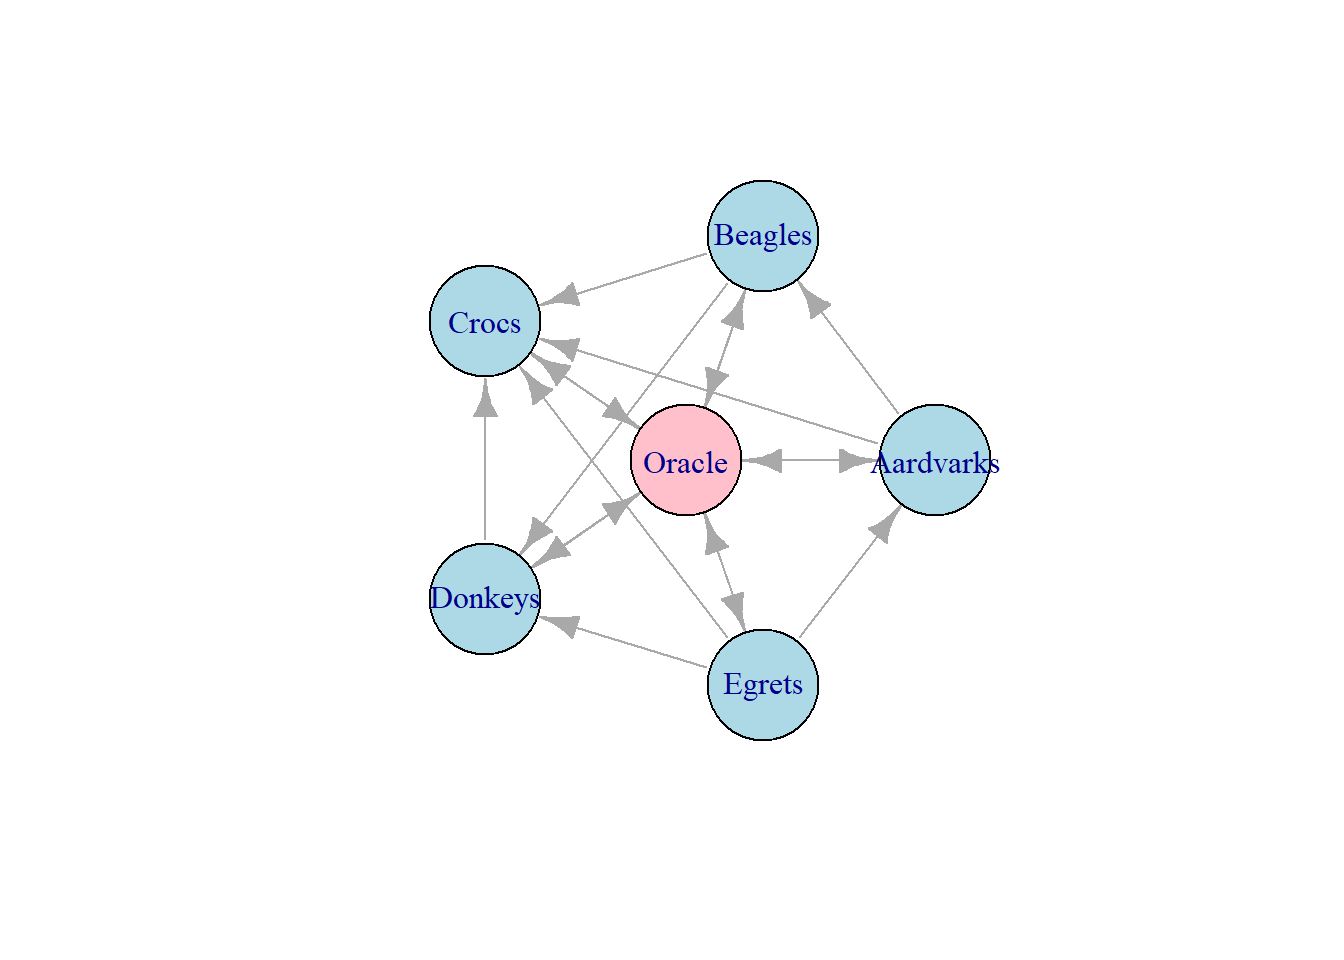
\includegraphics{_main_files/figure-latex/danglingoracle-1.pdf}
\caption{\label{fig:danglingoracle}The Oracle}
\end{figure}

By adjusting the number of edges up to and down from the Oracle, we can fine tune the ratings. The simplest case just has 1 edge in both directions. The original transposed adjacency matrix and Oracle adjacency matrix will look like this.

\[\mathbf{A}=\begin{bmatrix} 0 & 0 & 0 & 0 & 1 \\ 
   1 & 0 & 0 & 0 & 0 \\ 
   1 & 1 & 0 & 1 & 1 \\ 
   0 & 1 & 0 & 0 & 1 \\ 
   0 & 0 & 0 & 0 & 0 \end{bmatrix},\mathbf{A}_{Oracle}=\begin{bmatrix} 0 & 0 & 0 & 0 & 1 & \mathbf{1} \\ 
   1 & 0 & 0 & 0 & 0 & \mathbf{1} \\ 
   1 & 1 & 0 & 1 & 1 & \mathbf{1} \\ 
   0 & 1 & 0 & 0 & 1 & \mathbf{1} \\ 
   0 & 0 & 0 & 0 & 0 & \mathbf{1} \\ 
   \mathbf{1} & \mathbf{1} & \mathbf{1} & \mathbf{1} & \mathbf{1} & \mathbf{0}\end{bmatrix}\]

When we divide by the column sums, we get the transition matrix with the Oracle:

\[\mathbf{S=}\begin{bmatrix} 0 & 0 & 0 & 0 & 1/4 & 1/5 \\ 1/3 & 0 & 0 & 0 & 0 & 1/5\\
  1/3 & 1/3 & 0 & 1/2 & 1/4 & 1/5 \\ 
   0 & 1/3 & 0 & 0 & 1/4 & 1/5 \\ 
   0 & 0 & 0 & 0 & 0 & 1/5 \\ 
  1/3 & 1/3 & 1 & 1/2 & 1/4 & 0\end{bmatrix}\]

When we exponentiate \(\mathbf{S}\), all of the columns look like this, where the last entry belongs to the Oracle.

\[(0.0933610, 0.1058091, 0.2240664, 0.1286307, 0.0746888, 0.3734440)\]

If we remove the Oracle and rescale the remaining ratings to add to 1 (not necessary, but otherwise the numbers can be quite small), we get the following ranking:

\begin{longtable}[]{@{}lllll@{}}
\toprule\noalign{}
\textbf{Team} & W & L & Rating & Rank \\
\midrule\noalign{}
\endhead
\bottomrule\noalign{}
\endlastfoot
\textbf{Crocs} & 4 & 0 & 0.358 & 1 \\
\textbf{Donkeys} & 2 & 1 & 0.205 & 2 \\
\textbf{Beagles} & 1 & 2 & 0.169 & 3 \\
\textbf{Aardvarks} & 1 & 2 & 0.149 & 4 \\
\textbf{Egrets} & 0 & 3 & 0.119 & 5 \\
\end{longtable}

\subsection*{Modifications}\label{modifications}
\addcontentsline{toc}{subsection}{Modifications}

The nice thing about the Oracle method is that the number of edges up to and down from the Oracle can be adjusted. Suppose the Oracle likes winners. The number of edges down to a team can be based on the number of wins they have. Because we need at least one edge down to every team, we add 1 to the win total. Here are the respective transposed adjacency matrix and transition matrix.

\[\textbf{A}_{Oracle}=\begin{bmatrix} 0 & 0 & 0 & 0 & 1 & 2 \\ 
   1 & 0 & 0 & 0 & 0 & 2 \\ 
   1 & 1 & 0 & 1 & 1 & 5 \\ 
   0 & 1 & 0 & 0 & 1 & 3 \\ 
   0 & 0 & 0 & 0 & 0 & 1 \\ 
 1 & 1 & 1 & 1 & 1 & 0\end{bmatrix},\textbf{S}=\begin{bmatrix} 0 & 0 & 0 & 0 & 1/4 & 2/13 \\ 1/3 & 0 & 0 & 0 & 0 & 2/13\\
  1/3 & 1/3 & 0 & 1/2 & 1/4 & 5/13 \\ 
   0 & 1/3 & 0 & 0 & 1/4 & 3/13 \\ 
   0 & 0 & 0 & 0 & 0 & 1/13 \\ 
  1/3 & 1/3 & 1 & 1/2 & 1/4 & 0\end{bmatrix}\]

Here are the resulting ratings. Note that the Crocs' rating has increased from 0.358 to 0.470, while the winless Egrets' rating has gone down significantly.

\begin{longtable}[]{@{}lllll@{}}
\toprule\noalign{}
\textbf{Team} & W & L & Rating & Rank \\
\midrule\noalign{}
\endhead
\bottomrule\noalign{}
\endlastfoot
\textbf{Crocs} & 4 & 0 & 0.470 & 1 \\
\textbf{Donkeys} & 2 & 1 & 0.217 & 2 \\
\textbf{Beagles} & 1 & 2 & 0.143 & 3 \\
\textbf{Aardvarks} & 1 & 2 & 0.117 & 4 \\
\textbf{Egrets} & 0 & 3 & 0.052 & 5 \\
\end{longtable}

\section{Exercises}\label{exercises-2}

\begin{enumerate}
\def\labelenumi{\arabic{enumi}.}
\item
  Let
  \[\mathbf{A}=\begin{bmatrix} 1 & 2\\5 & 4\end{bmatrix}.\]
  Find the eigenvalues and eigenvectors of \(\mathbf{A}\) by hand.
\item
  Let
  \[\mathbf{A}=\begin{bmatrix} 3 & 2\\5 & 0\end{bmatrix}.\]
  Find the eigenvalues and eigenvectors of \(\mathbf{A}\) by hand.
\item
  Let
  \[\mathbf{A}=\begin{bmatrix} 2 & -2\\2 & 6\end{bmatrix}.\]
  Find the eigenvalues and eigenvectors of \(\mathbf{A}\) by hand.
\item
  Let
  \[\mathbf{A}=\begin{bmatrix} 1 & 4\\-1 & 5\end{bmatrix}.\]
  Find the eigenvalues and eigenvectors of \(\mathbf{A}\) by hand.
\item
  The matrix
  \[\mathbf{A}=\begin{bmatrix} -2 & -3 & -1\\1 & 2 & 1\\3 & 3 & 2\end{bmatrix}\]
  has eigenvalues \(\lambda_1=2, \lambda_2=1,\) and \(\lambda_3=-1.\) Find the corresponding eigenvectors by hand.
\item
  The matrix
  \[\mathbf{A}=\begin{bmatrix} 2 & -1 & 1\\-1 & 2 & -1\\1 & 1 & 2\end{bmatrix}\]
  has eigenvalues \(\lambda_1=3, \lambda_2=2,\) and \(\lambda_3=-1.\) Find the corresponding eigenvectors by hand.
\item
  Find a nondiagonal, nontriangular \(2\times 2\) matrix that has eigenvalues \(\lambda_1=5\) and \(\lambda_2=-2.\)
\item
  Find a nondiagonal, nontriangular \(2\times 2\) matrix that has eigenvalues \(\lambda_1=4\) and \(\lambda_2=3.\)
\item
  For the matrix in Problem 1, show that the nonzero columns of \(\mathbf{A}-\lambda_1\mathbf{I}\) are eigenvectors corresponding to \(\lambda_2\) and that the nonzero columns of \(\mathbf{A}-\lambda_2\mathbf{I}\) are eigenvectors corresponding to \(\lambda_1.\) (This is a general result for \(2\times 2\) matrices with non-repeating real eigenvalues.)
\item
  For the matrix in Problem 2, show that the nonzero columns of \(\mathbf{A}-\lambda_1\mathbf{I}\) are eigenvectors corresponding to \(\lambda_2\) and that the nonzero columns of \(\mathbf{A}-\lambda_2\mathbf{I}\) are eigenvectors corresponding to \(\lambda_1.\)
\item
  The matrix \(\mathbf{A}=\begin{bmatrix}2 & 3\\3&2\end{bmatrix}\) found in Example \ref{exm:ndnt} has the eigenvector \(\mathbf{x}_1=\begin{bmatrix}1\\1\end{bmatrix}\) corresponding to the eigenvalue \(\lambda_1=5.\) Find \(\mathbf{A}^{3}\mathbf{x}_1.\)
\item
  The matrix \(\mathbf{A}=\begin{bmatrix}2 & 3\\3&2\end{bmatrix}\) found in Example \ref{exm:ndnt} has the eigenvector \(\mathbf{x}_2=\begin{bmatrix}-1\\1\end{bmatrix}\) corresponding to the eigenvalue \(\lambda_2=-1.\) Find \(\mathbf{A}^{101}\mathbf{x}_2.\)
\item
  Let \(\mathbf{L}=\begin{bmatrix} 2.9 & 3\\0.1 & 0\end{bmatrix}\) be a Leslie matrix. Suppose an initial population distribution of \(\mathbf{N}(0)=\begin{bmatrix}10 \\0\end{bmatrix}.\)

  \begin{enumerate}
  \def\labelenumii{\alph{enumii}.}
  \tightlist
  \item
    Find \(\mathbf{N}(1)\) and \(\mathbf{N}(2).\) Do not round.
  \item
    Find the eigenvalues of \(\mathbf{L}.\)
  \item
    What is the long-run growth rate?
  \item
    What is the long-run ratio of age-zero to age-one individuals?
  \end{enumerate}
\item
  Let \(\mathbf{L}=\begin{bmatrix} 4.9 & 10\\0.05 & 0\end{bmatrix}\) be a Leslie matrix. Suppose an initial population distribution of \(\mathbf{N}(0)=\begin{bmatrix}100 \\0\end{bmatrix}.\)

  \begin{enumerate}
  \def\labelenumii{\alph{enumii}.}
  \tightlist
  \item
    Find \(\mathbf{N}(1)\) and \(\mathbf{N}(2).\) Do not round.
  \item
    Find the eigenvalues of \(\mathbf{L}.\)
  \item
    What is the long-run growth rate?
  \item
    What is the long-run ratio of age-zero to age-one individuals?
  \end{enumerate}
\item
  Let \(\mathbf{L}=\begin{bmatrix} 2 & 4 & 1\\0.05 & 0 & 0\\0 & 0.4 & 0\end{bmatrix}\) be a Leslie matrix. Suppose an initial population distribution of \(\mathbf{N}(0)=\begin{bmatrix}10 \\10\\10\end{bmatrix}.\)

  \begin{enumerate}
  \def\labelenumii{\alph{enumii}.}
  \tightlist
  \item
    Find \(\mathbf{N}(1)\) and \(\mathbf{N}(2).\) Do not round.
  \item
    Find the eigenvalues of \(\mathbf{L}.\)
  \item
    What is the long-run growth rate?
  \item
    In the long run, what will the percentages for each age group be?
  \end{enumerate}
\item
  Let \(\mathbf{L}=\begin{bmatrix} 5 & 6 & 2\\0.01 & 0 & 0\\0 & 0.2 & 0\end{bmatrix}\) be a Leslie matrix. Suppose an initial population distribution of \(\mathbf{N}(0)=\begin{bmatrix}10 \\10\\10\end{bmatrix}.\)

  \begin{enumerate}
  \def\labelenumii{\alph{enumii}.}
  \tightlist
  \item
    Find \(\mathbf{N}(1)\) and \(\mathbf{N}(2).\) Do not round.
  \item
    Find the eigenvalues of \(\mathbf{L}.\)
  \item
    What is the long-run growth rate?
  \item
    In the long run, what will the percentages for each age group be?
  \end{enumerate}
\item
  Let \(\mathbf{L}=\begin{bmatrix} 0 & 4\\ 0.5 & 0\end{bmatrix}\) be a Leslie matrix. Suppose an initial population distribution of \(\mathbf{N}(0)=\begin{bmatrix}2\\0\end{bmatrix}.\)

  \begin{enumerate}
  \def\labelenumii{\alph{enumii}.}
  \tightlist
  \item
    Find \(\mathbf{N}(1), \mathbf{N}(2), \mathbf{N}(3),\) and \(\mathbf{N}(4).\)
  \item
    Will there be a stable population distribution?
  \end{enumerate}
\item
  Let \(\mathbf{L}=\begin{bmatrix} 0 & 8\\ 0.25 & 0\end{bmatrix}\) be a Leslie matrix. Suppose an initial population distribution of \(\mathbf{N}(0)=\begin{bmatrix}0\\2\end{bmatrix}.\)

  \begin{enumerate}
  \def\labelenumii{\alph{enumii}.}
  \tightlist
  \item
    Find \(\mathbf{N}(1), \mathbf{N}(2), \mathbf{N}(3),\) and \(\mathbf{N}(4).\)
  \item
    Will there be a stable population distribution?
  \end{enumerate}
\item
  Sketch an undirected graph with adjacency matrix
  \[\mathbf{A}=\begin{bmatrix} 1 & 1 & 2 & 0\\1 & 0 & 1 & 1\\2 & 1 & 0 & 0\\0 & 1 & 0 & 0\end{bmatrix}.\]
\item
  Sketch an undirected graph with adjacency matrix
  \[\mathbf{A}=\begin{bmatrix} 0 & 0 & 1 & 1\\0 & 1 & 2 & 0\\1 & 2 & 0 & 2\\1 & 0 & 2 & 0\end{bmatrix}.\]
\item
  For the graph in Problem 19, how many ways are there to get from vertex 1 to vertex 2 in exactly four steps?
\item
  For the graph in Problem 20, how many ways are there to get from vertex 1 to vertex 3 in exactly five steps?
\item
  Find the adjacency matrix for the directed graph in Figure \ref{fig:p23}.
\end{enumerate}

\begin{figure}

{\centering 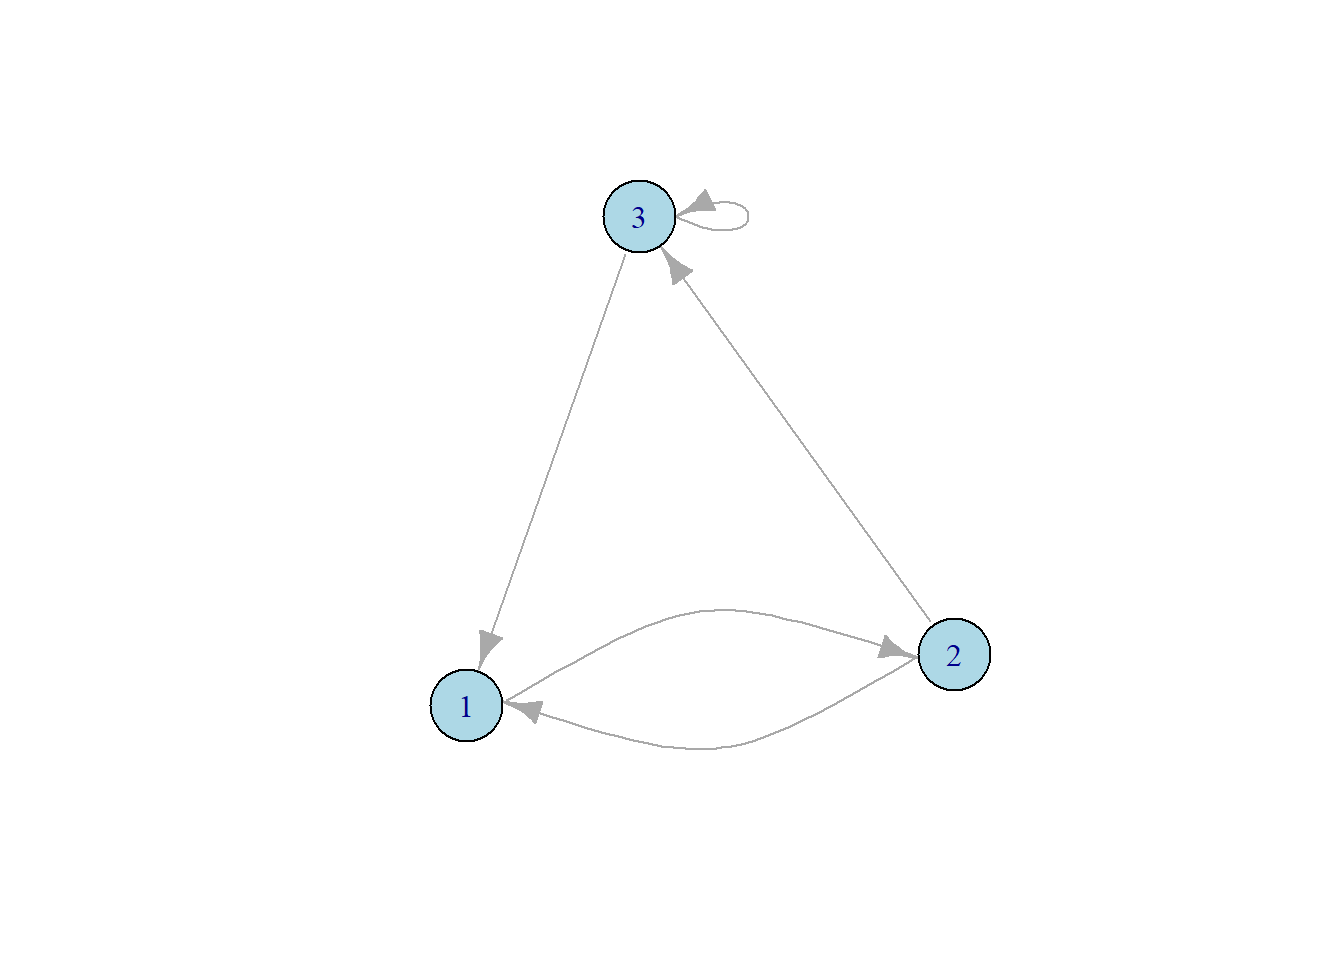
\includegraphics[width=0.6\linewidth]{_main_files/figure-latex/p23-1} 

}

\caption{Graph for Problem 23}\label{fig:p23}
\end{figure}

\begin{enumerate}
\def\labelenumi{\arabic{enumi}.}
\setcounter{enumi}{23}
\tightlist
\item
  Find the adjacency matrix for the directed graph in Figure \ref{fig:p24}.
\end{enumerate}

\begin{figure}

{\centering 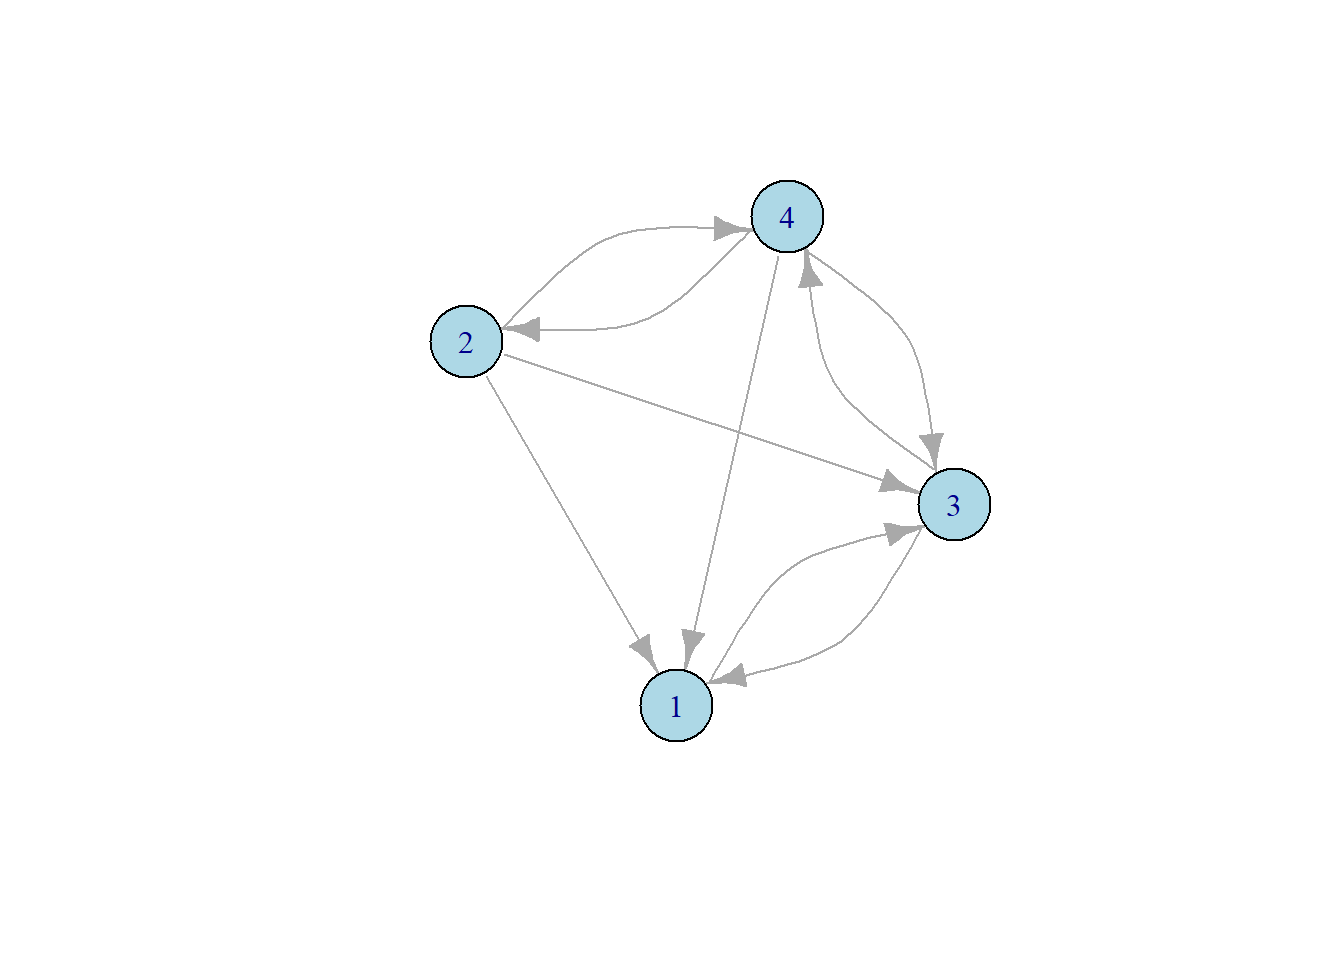
\includegraphics[width=0.6\linewidth]{_main_files/figure-latex/p24-1} 

}

\caption{Graph for Problem 24}\label{fig:p24}
\end{figure}

\begin{enumerate}
\def\labelenumi{\arabic{enumi}.}
\setcounter{enumi}{24}
\tightlist
\item
  Find the column stochastic transition matrix for the graph in Figure \ref{fig:p25}.
\end{enumerate}

\begin{figure}

{\centering 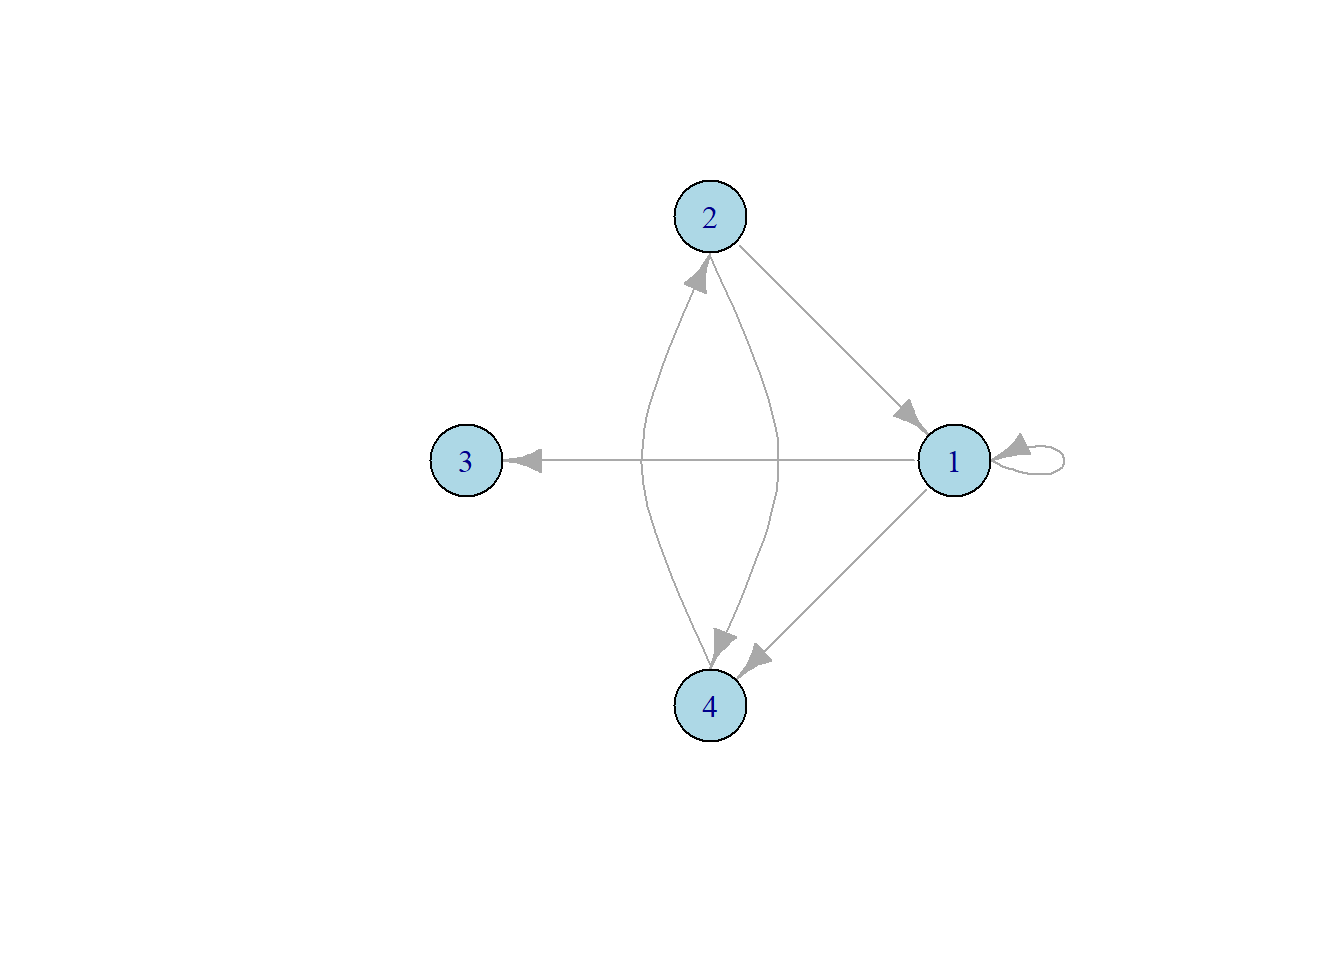
\includegraphics[width=0.6\linewidth]{_main_files/figure-latex/p25-1} 

}

\caption{Graph for Problem 25}\label{fig:p25}
\end{figure}

\begin{enumerate}
\def\labelenumi{\arabic{enumi}.}
\setcounter{enumi}{25}
\tightlist
\item
  Find the column stochastic transition matrix for the graph in Figure \ref{fig:p26}.
\end{enumerate}

\begin{figure}

{\centering 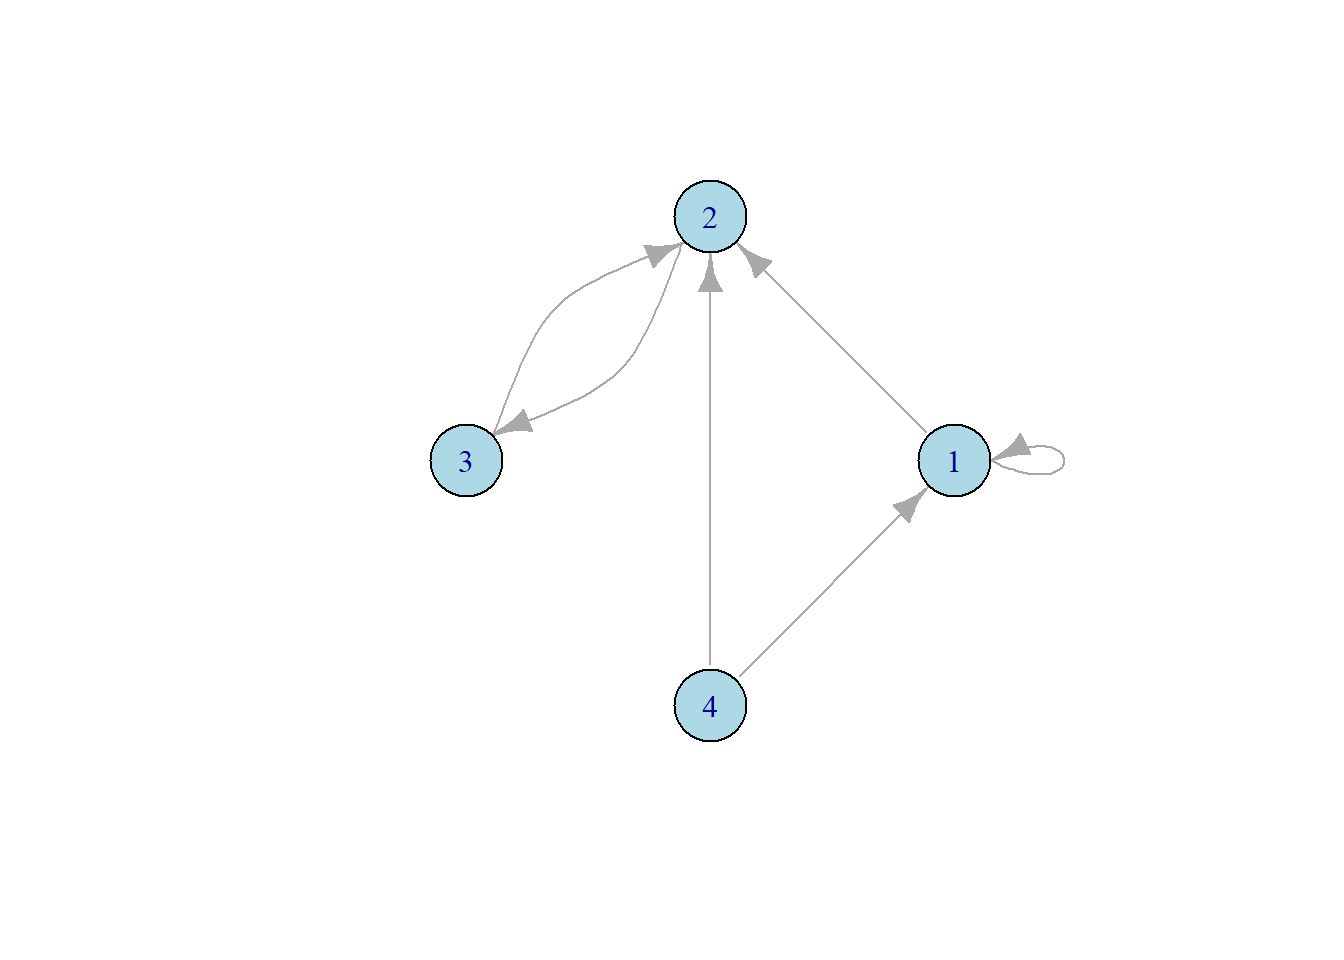
\includegraphics[width=0.6\linewidth]{_main_files/figure-latex/p26-1} 

}

\caption{Graph for Problem 26}\label{fig:p26}
\end{figure}

\begin{enumerate}
\def\labelenumi{\arabic{enumi}.}
\setcounter{enumi}{26}
\tightlist
\item
  A switch has two positions: on and off. Every second, the position might change. If it is in the on position, it changes to off with probability 2/3, and stays on with probability 1/3. If it is in the off position, it switches to on with probability 1/2 and stays off with probability 1/2.

  \begin{enumerate}
  \def\labelenumii{\alph{enumii}.}
  \tightlist
  \item
    Write out the column stochastic transition matrix for this switch.
  \item
    If the switch is on now, what is the probability that it is on two seconds from now? (That is, after two switching opportunities.)
  \item
    What percentage of the time is the switch in the on position?
  \end{enumerate}
\item
  Professor X holds random office hours. If he holds office hours one day, the probability he holds them the next day is 1/10. If he does not hold them one day, the probability he holds them the next day is 1/2.

  \begin{enumerate}
  \def\labelenumii{\alph{enumii}.}
  \tightlist
  \item
    Write out the column stochastic transition matrix for Professor X's office hours.
  \item
    If Professor X holds office hours today, what is the probability he holds office hours two days from now?
  \item
    In the long run, what fraction of days does Professor X hold office hours?
  \end{enumerate}
\item
  In the Chapter 1 Exercises, we found the Colley ratings based on some football results. We are now going to apply the Markov method to those same results. Based on the results below (Problem 39 from Chapter 1), perform the following.

  \begin{itemize}
  \tightlist
  \item
    Write out the column stochastic transition matrix \(\mathbf{T}.\)
  \item
    The Argos didn't lose. Adjust for this \emph{dangling node} to get a new matrix \(\mathbf{S}.\)
  \item
    Find \(\mathbf{G}=0.85\mathbf{S}+0.15\mathbf{E},\) where \(\mathbf{E}\) is the teleportation matrix.
  \item
    Find the ratings by finding the probability vector guaranteed by the Perron-Frobenius Theorem.
  \end{itemize}
\end{enumerate}

\begin{longtable}{lrlr}
\toprule
Winner & Score & Loser & Score\\
\midrule
Argos & 20 & Brahmas & 13\\
Cobbers & 31 & Brahmas & 10\\
Argos & 24 & Cobbers & 21\\
Dukes & 10 & Brahmas & 7\\
Brahmas & 35 & Dukes & 3\\
\bottomrule
\end{longtable}

\begin{enumerate}
\def\labelenumi{\arabic{enumi}.}
\setcounter{enumi}{29}
\tightlist
\item
  Let's find the Markov ratings for the results in Problem 40 from Chapter 1. Perform the following.

  \begin{itemize}
  \tightlist
  \item
    Write out the column stochastic transition matrix \(\mathbf{T}.\)
  \item
    Adjust for any dangling nodes to get the matrix \(\mathbf{S}.\) (If there are no dangling nodes, then \(\mathbf{S}=\mathbf{T}\).)
  \item
    Find \(\mathbf{G}=0.85\mathbf{S}+0.15\mathbf{E},\) where \(\mathbf{E}\) is the teleportation matrix.
  \item
    Find the ratings by finding the probability vector guaranteed by the Perron-Frobenius Theorem.
  \end{itemize}
\end{enumerate}

\begin{longtable}{lrlr}
\toprule
Winner & Score & Loser & Score\\
\midrule
Argos & 28 & Cobbers & 14\\
Brahmas & 21 & Argos & 13\\
Brahmas & 17 & Dukes & 10\\
Dukes & 31 & Brahmas & 28\\
\bottomrule
\end{longtable}

\begin{enumerate}
\def\labelenumi{\arabic{enumi}.}
\setcounter{enumi}{30}
\tightlist
\item
  Now, let's apply the Oracle method to the results in Problem 29.

  \begin{itemize}
  \tightlist
  \item
    Find the transposed adjacency matrix \(\mathbf{A}.\)
  \item
    Add a column for the Oracle by summing each row and adding 1. This will represent the number of wins for each team, increased by 1.
  \item
    Add a row for the Oracle at the bottom. This row will consist of four ones and a zero at the end.
  \item
    Make this new matrix column stochastic by dividing each column by its sum.
  \item
    Find the Oracle ratings by finding the probability eigenvector.
  \end{itemize}
\item
  Find the Oracle ratings for the results in Problem 30. Use the instructions in Problem 31.
\end{enumerate}

\chapter{Orthogonality}\label{orthogonality}

Several of our future topics will rely heavily on a property called \emph{orthogonality}. These topics include least squares, the singular value decomposition, and principal component analysis. In this chapter, we will lay the groundwork for those discussions.

\section{Inner Product, Length, and Orthogonality}\label{ILO}

Now we want to define the \emph{inner product}\index{Inner product} of two vectors.

\begin{defbox}

\begin{definition}
Let \(\mathbf{u}\) and \(\mathbf{v}\) be vectors in \(\mathbb{R}^n\), with

\[\mathbf{u}=\begin{bmatrix}u_1\\u_2\\\vdots\\u_n\end{bmatrix},\mathbf{v}=\begin{bmatrix}v_1\\v_2\\\vdots\\v_n\end{bmatrix}.\]

Then the \textbf{inner} or \textbf{dot product}\index{Dot product!as an inner product} of \(\mathbf{u}\) and \(\mathbf{v}\), denoted \(\mathbf{u}\cdot\mathbf{v}\) is

\[\mathbf{u}\cdot\mathbf{v}=\mathbf{u}^T\mathbf{v}=\begin{bmatrix}u_1 & u_2 & \cdots & u_n\end{bmatrix}\begin{bmatrix}v_1\\v_2\\\vdots\\v_n\end{bmatrix}=u_1v_1+u_2v_2+\cdots+u_nv_n.\]
\end{definition}

\end{defbox}

We've already mentioned the dot product when we defined matrix multiplication, but now we are going to see a few more of its properties. The ability to write it as a matrix product involving the transpose of one of the vectors is particularly useful.

\pagebreak

\begin{examplebox}

\begin{example}
With

\[\mathbf{u}=\begin{bmatrix}1\\-2\\3\end{bmatrix},\mathbf{v}=\begin{bmatrix}4\\7\\5\end{bmatrix},\]

we have

\[\mathbf{u}\cdot\mathbf{v}=(1)(4)+(-2)(7)+(3)(5)=5.\]
\end{example}

\end{examplebox}

Note that by commutativity of multiplication, \(\mathbf{u}\cdot \mathbf{v}=\mathbf{v}\cdot\mathbf{u}\). Here is a larger list of the properties.

\begin{theorembox}

\begin{theorem}

Let \(\mathbf{u}, \mathbf{v},\) and \(\mathbf{w}\) be vectors in \(\mathbb{R}^n\), and let \(c\) be a scalar. Then

\begin{enumerate}
\def\labelenumi{\arabic{enumi}.}
\item
  \(\mathbf{u}\cdot \mathbf{v}=\mathbf{v}\cdot \mathbf{u}\)
\item
  \((\mathbf{u}+\mathbf{v})\cdot \mathbf{w}=\mathbf{u}\cdot \mathbf{w}+\mathbf{v}\cdot \mathbf{w}\)
\item
  \((c\mathbf{u})\cdot \mathbf{v}=c(\mathbf{u}\cdot \mathbf{v})=\mathbf{u}\cdot(c\mathbf{v})\)
\item
  \(\mathbf{u}\cdot \mathbf{u}\geq 0\), and \(\mathbf{u}\cdot\mathbf{u}=0\) if and only if \(\mathbf{u}=\mathbf{0}.\)
\end{enumerate}

\end{theorem}

\end{theorembox}

The last property holds because if \(\mathbf{u}=(u_1,u_2,\dots,u_n)\), then

\[\mathbf{u}\cdot \mathbf{u}=u_1u_1+u_2u_2+\cdots+u_nu_n=u_1^2+u_2^2+\cdots+u_n^2,\]

which is never negative, and can only be zero if all the \(u_i\) are zero. You should recognize \(\mathbf{u}\cdot \mathbf{u}\) as the magnitude of \(\mathbf{u}\) squared.

\begin{theorembox}

\begin{theorem}
Let \(\mathbf{v}\) be a vector in \(\mathbb{R}^n\). The magnitude\index{Magnitude} or \emph{norm}\index{Norm} of \(\mathbf{v}\) is

\[|\mathbf{v}|=\sqrt{\mathbf{v}\cdot \mathbf{v}}=\sqrt{v_1^2+v_2^2+\cdots+v_n^2},\]

and

\[\mathbf{v}\cdot \mathbf{v}=\mathbf{v}^T\mathbf{v}=|\mathbf{v}|^2.\]
\end{theorem}

\end{theorembox}

If we multiply a vector by a constant \(c\), how does its length change?

\[|c\mathbf{v}|=\sqrt{c^2v_1^2+c^2v_2^2+\cdots+c^2v_n^2}=\sqrt{c^2(v_1^2+v_2^2+\cdots +v_n^2)}=|c||\mathbf{v}|.\]

A \emph{unit vector}\index{Unit vector} is a vector whose length is 1. They are handy things to have. If \(\mathbf{v}\) is a nonzero vector, then

\[\mathbf{u}=\frac{1}{|\mathbf{v}|}\mathbf{v}\]

is a unit vector in the direction of \(\mathbf{v}\).

\begin{examplebox}

\begin{example}
Let \(\mathbf{v}=(2,-1,3).\) Find a unit vector in the direction of \(\mathbf{v}.\)

With \(|\mathbf{v}|=\sqrt{2^2+(-1)^2+3^2}=\sqrt{4+1+9}=\sqrt{14}\), we have

\[\mathbf{u}=\frac{1}{\sqrt{14}}(2,-1,3)=\left(\frac{2}{\sqrt{14}},-\frac{1}{\sqrt{14}},\frac{3}{\sqrt{14}}\right).\]

Let's check:

\[|\mathbf{u}|^2=\frac{4}{14}+\frac{1}{14}+\frac{9}{14}=1,\]

so \(|\mathbf{u}|=1\).
\end{example}

\end{examplebox}

\subsection*{\texorpdfstring{Distance in \(\mathbb{R}^n\)}{Distance in \textbackslash mathbb\{R\}\^{}n}}\label{distance-in-mathbbrn}
\addcontentsline{toc}{subsection}{Distance in \(\mathbb{R}^n\)}

Let \(\mathbf{u}=(u_1,u_2,\dots,u_n)\) and \(\mathbf{v}=(v_1,v_2,\dots,v_n)\) be vectors in \(\mathbb{R}^n\). Then the distance between (the tips of) \(\mathbf{u}\) and \(\mathbf{v}\) is given by the distance formula\index{Distance formula}:

\begin{align*}
\text{dist}(\mathbf{u},\mathbf{v})&=\sqrt{(u_1-v_1)^2+(u_2-v_2)^2+\cdots+(u_n-v_n)^2}\\
&=\sqrt{(\mathbf{u}-\mathbf{v})\cdot (\mathbf{u}-\mathbf{v})}\\
&=|\mathbf{u}-\mathbf{v}|.
\end{align*}

The inner product between two vectors tells us something about their relationship. The following theorem gives us that relationship.

\begin{theorembox}

\begin{theorem}
Let \(\mathbf{u}\) and \(\mathbf{v}\) be two vectors in \(\mathbb{R}^n\). Then

\begin{equation}
\mathbf{u}\cdot\mathbf{v}=|\mathbf{u}||\mathbf{v}|\cos\theta,
\label{eq:lawofcosines}
\end{equation}

where \(\theta\) is the angle between \(\mathbf{u}\) and \(\mathbf{v}.\)
\end{theorem}

\end{theorembox}

Equation \eqref{eq:lawofcosines} is often called the \emph{Law of Cosines}, and you can derive it from that trigonometric equation. Note that if \(\mathbf{u}\) and \(\mathbf{v}\) are perpendicular, then \(\theta=90^\circ, \cos\theta=0,\) and \(\mathbf{u}\cdot \mathbf{v}=0.\) Similarly, if \(\mathbf{u}\) and \(\mathbf{v}\) are nonzero vectors and \(\theta\neq 90^\circ,\) then \(\mathbf{u}\cdot \mathbf{v}\neq 0\).

\begin{defbox}

\begin{definition}
Two vectors \(\mathbf{u}\) and \(\mathbf{v}\) are \textbf{orthogonal}\index{Orthogonality!of vectors} if \(\mathbf{u}\cdot\mathbf{v}=0.\)
\end{definition}

\end{defbox}

Here are some examples.

\begin{itemize}
\tightlist
\item
  Let \(\mathbf{u}=(1,3,2)\) and \(\mathbf{v}=(2,4,1)\). Then
\end{itemize}

\[\mathbf{u}\cdot \mathbf{v}=2+12+2=16,\]

so \(\mathbf{u}\) and \(\mathbf{v}\) are not orthogonal.

\begin{itemize}
\tightlist
\item
  Let \(\mathbf{u}=(1,3,2)\) and \(\mathbf{v}=(2,4,-7)\). Then
\end{itemize}

\[\mathbf{u}\cdot \mathbf{v}=2+12-14=0\]

and \(\mathbf{u}\) and \(\mathbf{v}\) are orthogonal.

\begin{itemize}
\tightlist
\item
  Note that \(\mathbf{v}\cdot\mathbf{0}=0\) for any vector \(\mathbf{v}\), so the zero vector is orthogonal to every vector.
\end{itemize}

\section{Orthogonal Subspaces}\label{orthogonal-subspaces}

Remember subspaces? Important examples included the column, row, and null space of a matrix \(\mathbf{A}\). We can consider vectors that are \emph{orthogonal} to these subspaces.

\begin{defbox}

\begin{definition}
Let \(W\) be a subspace of \(\mathbb{R}^n\) and let \(\mathbf{v}\) be a vector in \(\mathbb{R}^n\). We say that \(\mathbf{v}\) is \textbf{orthogonal}\index{Orthogonality!of subspaces} to \(W\) if
\(\mathbf{v}\) is orthogonal to every vector in \(W\). The \emph{orthogonal complement}\index{Orthogonal!complement} of \(W\) is the collection of all vectors orthogonal to \(W\), and is denoted \(W^{\perp}\) (read as ``\(W\)-perp'').
\end{definition}

\end{defbox}

The following theorems are useful.

\begin{theorembox}

\begin{theorem}
Let \(W\) be a subspace of \(\mathbb{R}^n\). A vector \(\mathbf{x}\) is in \(W^\perp\) if and only if \(\mathbf{x}\) is orthogonal to every vector in a set that spans \(W\).
\end{theorem}

\end{theorembox}

This means we can check it against a basis or any convenient spanning set. The next one tells us the structure of \(W^{\perp}.\)

\begin{theorembox}

\begin{theorem}
Let \(W\) be a subspace of \(\mathbb{R}^n\). Then \(W^\perp\) is a subspace of \(\mathbb{R}^n\).
\end{theorem}

\end{theorembox}

\subsection*{The row space and nullspace of a matrix}\label{the-row-space-and-nullspace-of-a-matrix}
\addcontentsline{toc}{subsection}{The row space and nullspace of a matrix}

We can actually write \(\mathbb{R}^n\) in terms of some special orthogonal subspaces. Recall that the row space of an \(m\times n\) matrix \(\mathbf{A}\) is the span of its row vectors, while the nullspace of \(\mathbf{A}\) is the set of all vectors \(\mathbf{v}\) such that \(\mathbf{A}\mathbf{v}=\mathbf{0}\).

Suppose \(\mathbf{v}=(v_1,v_2,\dots,v_n)\) is in \(\text{Null}(\mathbf{A})\). Then, focusing on the second row of \(\mathbf{A}\) as an example,

\[\mathbf{A}\mathbf{v}=\begin{bmatrix} &  &  & \\a_{21} & a_{22} & \cdots & a_{2n}\\
&&&\\ &  &  & \end{bmatrix}\begin{bmatrix}v_1\\v_2\\\vdots \\v_n\end{bmatrix}=\begin{bmatrix}0\\\mathbf{0}\\ \vdots \\ 0\end{bmatrix}.\]

The \(i\)th entry in the product is the product of the \(i\)th row of \(\mathbf{A}\) with \(\mathbf{v}\). This means that \(\mathbf{v}\) is orthogonal to each row vector of \(\mathbf{A}\). Since the rows of \(\mathbf{A}\) span the row space of \(\mathbf{A}\), every vector in \(\text{Null}(\mathbf{A})\) is in \(\text{Row}(\mathbf{A})^{\perp}\).

We get the following theorem.

\begin{theorembox}

\begin{theorem}
\protect\hypertarget{thm:MatSubspaces}{}\label{thm:MatSubspaces}Let \(\mathbf{A}\) be an \(m\times n\) matrix. Then

\[(\textrm{Row}(\mathbf{A}))^\perp=\textrm{Null}(\mathbf{A})\]

and

\[(\textrm{Col}(\mathbf{A}))^{\perp}=\textrm{Null}(\mathbf{A}^T).\]
\end{theorem}

\end{theorembox}

The second statement is true because the columns of \(\mathbf{A}\) become the rows of \(\mathbf{A}^T\). These theorems seem a little abstract now, but they will come in handy in the future.

\section{Orthogonal and Orthonormal Sets}\label{orthogonal-and-orthonormal-sets}

In Section \ref{ILO}, we defined what it meant for two vectors to be orthogonal. In this section, we're going to talk about sets of mutually orthogonal vectors. First, a definition.

\begin{defbox}

\begin{definition}
A set of vectors \(\{\mathbf{u}_1,\mathbf{u}_2,\dots,\mathbf{u}_p\}\) in \(\mathbb{R}^n\) is said to be an \textbf{orthogonal set}\index{Orthogonality!of sets} if each pair of distinct vectors from the set is orthogonal, that is, if \(\mathbf{u}_i\cdot\mathbf{u}_j=0\) whenever \(i\neq j\).
\end{definition}

\end{defbox}

\begin{examplebox}

\begin{example}
\protect\hypertarget{exm:orthoset}{}\label{exm:orthoset}If

\[\mathbf{u}_1=\begin{bmatrix}3\\1\\1\end{bmatrix},\mathbf{u}_2=\begin{bmatrix}-1\\2\\1\end{bmatrix},\text{ and }\mathbf{u}_3=\begin{bmatrix}-1\\-4\\7\end{bmatrix},\]

we have

\[\mathbf{u}_1\cdot \mathbf{u}_2=(3)(-1)+(1)(2)+(1)(1)=0,\]

\[\mathbf{u}_1\cdot\mathbf{u}_3=(3)(-1)+(1)(-4)+(1)(7)=0,\]

and

\[\mathbf{u}_2\cdot \mathbf{u}_3=(-1)(-1)+(2)(-4)+(1)(7)=0.\]
\end{example}

\end{examplebox}

It shouldn't be surprising that orthogonal sets are linearly independent. Here's a theorem.

\begin{theorembox}

\begin{theorem}
If \(S=\{\mathbf{u}_1,\mathbf{u}_2,\cdots,\mathbf{u}_p\}\) is an orthogonal set of nonzero vectors in \(\mathbb{R}^n\), then \(S\) is linearly independent and hence is a basis for the subspace spanned by \(S\).
\end{theorem}

\end{theorembox}

\begin{proof}
We want to show that any linear combination that yields the zero vector is trivial. Suppose that

\[\mathbf{0}=c_1\mathbf{u}_1+c_2\mathbf{u}_2+\cdots+c_p\mathbf{u}_p.\]

Then

\begin{align*}
0=\mathbf{u}_1\cdot \mathbf{0}&=\mathbf{u}_1\cdot(c_1\mathbf{u}_1+c_2\mathbf{u}_2+\cdots+c_p\mathbf{u}_p)\\
&=c_1\mathbf{u}_1\cdot\mathbf{u}_1+c_2\mathbf{u}_1\cdot\mathbf{u}_2+\cdots+c_p\mathbf{u}_1\cdot\mathbf{u}_p\\
&=c_1|\mathbf{u}_1|^2+0+\cdots+0\\
&=c_1|\mathbf{u}_1|^2.
\end{align*}

Since \(\mathbf{u}_1\) is nonzero, its length is not zero, so \(c_1=0\). Similarly, \(c_2=c_3=\cdots=c_p=0.\) The only linear combination of the orthogonal set that yields the zero vector is indeed the trivial one, meaning \(S\) is linearly independent. Because \(S\) is linearly independent, it forms a basis for its span.
\end{proof}

Orthogonal \emph{bases} are nice things to have.

\begin{defbox}

\begin{definition}
An \textbf{orthogonal basis}\index{Orthogonal!basis} for a subspace \(W\) of \(\mathbb{R}^n\) is a basis for \(W\) that is also an orthogonal set.
\end{definition}

\end{defbox}

Note that the standard basis

\[\mathbf{e}_1=\begin{bmatrix}1\\0\\0\\\vdots\\0\end{bmatrix},\mathbf{e}_2=\begin{bmatrix}0 \\1\\0\\\vdots\\0\end{bmatrix},\cdots,\mathbf{e}_n=\begin{bmatrix}0\\0\\0\\\vdots\\1\end{bmatrix}\]

is an orthogonal basis for \(\mathbb{R}^n\).

When a basis is orthogonal, it's easy to find a linear combination of the basis vectors that yields any vector.

\begin{theorembox}

\begin{theorem}
\protect\hypertarget{thm:orthobasis}{}\label{thm:orthobasis}Let \(\{\mathbf{u}_1,\cdots,\mathbf{u}_p\}\) be an orthogonal basis for a subspace \(W\) of \(\mathbb{R}^n\). For each \(\mathbf{y}\) in \(W\), the weights (coefficients) in the linear combination

\[\mathbf{y}=c_1\mathbf{u}_1+\cdots+c_p\mathbf{u}_p\]

are given by

\[c_j=\frac{\mathbf{y}\cdot \mathbf{u}_j}{\mathbf{u}_j\cdot \mathbf{u}_j},j=1\dots p.\]
\end{theorem}

\end{theorembox}

The proof is similar to the last proof. The dot product of \(\mathbf{y}\) with each \(\mathbf{u}_j\) will tell you what each \(c_j\) has to be.

\begin{examplebox}

\begin{example}
In Example \ref{exm:orthoset},

\[S=\{\mathbf{u}_1,\mathbf{u}_2,\mathbf{u}_3\}=\left\{\begin{bmatrix}3\\1\\1\end{bmatrix},\begin{bmatrix}-1\\2\\1\end{bmatrix},\begin{bmatrix}-1\\-4\\7\end{bmatrix}\right\}\]

is an orthogonal basis for \(\mathbb{R}^3\). If \(\mathbf{y}=(1,2,3)\),

\[\mathbf{y}\cdot \mathbf{u}_1=8,\mathbf{y}\cdot \mathbf{u}_2=6, \text{ and } \mathbf{y}\cdot \mathbf{u}_3=12,\]

while

\[\mathbf{u}_1\cdot \mathbf{u}_1=11,\mathbf{u}_2\cdot\mathbf{u}_2=6,\text{ and }\mathbf{u}_3\cdot\mathbf{u}_3=66.\]

After simplifying fractions, we get

\[\mathbf{y}=\frac{8}{11}\mathbf{u}_1+\mathbf{u}_2+\frac{2}{11}\mathbf{u}_3.\]
\end{example}

\end{examplebox}

\subsection*{Orthogonal projections}\label{orthogonal-projections}
\addcontentsline{toc}{subsection}{Orthogonal projections}

Given a vector \(\mathbf{y}\) and another vector \(\mathbf{u}\), we'd like to be able to write

\[\mathbf{y}=\hat{\mathbf{y}}+\mathbf{z},\]

where \(\hat{\mathbf{y}}\)\index{Orthogonal!projection} is a vector in the same direction as \(\mathbf{u}\), and \(\mathbf{z}\) is a vector that is orthogonal to \(\mathbf{u}\) (Fig. \ref{fig:vproj}).

\begin{figure}

{\centering 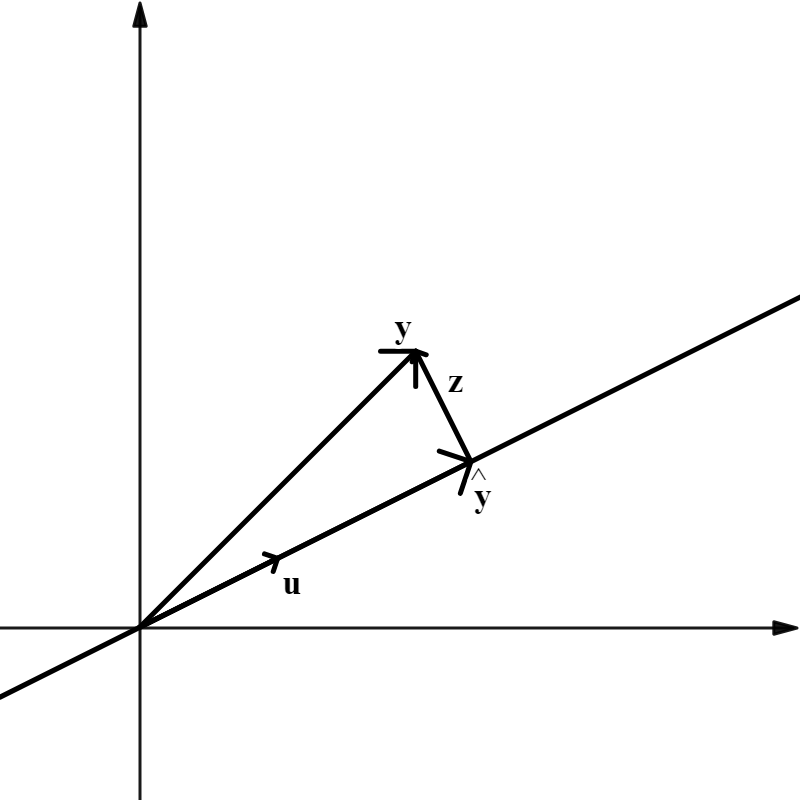
\includegraphics[width=0.5\linewidth]{images/vproj1} 

}

\caption{A vector projection}\label{fig:vproj}
\end{figure}

Our projection \(\hat{\mathbf{y}}\) will be some scalar multiple of \(\mathbf{u}\), say \(\hat{\mathbf{y}}=\alpha \mathbf{u}\). Then, since \(\mathbf{z}=\mathbf{y}-\hat{\mathbf{y}}=\mathbf{y}-\alpha\mathbf{u}\) should be orthogonal to \(\mathbf{u}\), we have

\[0=(\mathbf{y}-\alpha\mathbf{u})\cdot\mathbf{u}=\mathbf{y}\cdot\mathbf{u}-\alpha\mathbf{u}\cdot \mathbf{u}.\]

Solving for \(\alpha\) gives us our formula:

\begin{equation}
\hat{\mathbf{y}}=\text{proj}_L\mathbf{y}=\frac{\mathbf{y}\cdot\mathbf{u}}{\mathbf{u}\cdot \mathbf{u}}\mathbf{u},\label{eq:vproj}
\end{equation}

where \(\text{proj}_L\mathbf{y}\) refers to the projection of \(\mathbf{y}\) onto the line \(L\) spanned by \(\mathbf{u}\).

\begin{examplebox}

\begin{example}
Let \(\mathbf{u}=\begin{bmatrix}1\\3\end{bmatrix}\) and \(\mathbf{y}=\begin{bmatrix}4\\4\end{bmatrix}\). Then

\[\hat{\mathbf{y}}=\frac{(4,4)\cdot (1,3)}{(1,3)\cdot(1,3)}\begin{bmatrix}1\\3\end{bmatrix}=\frac{16}{10}\begin{bmatrix}1\\3\end{bmatrix}=\begin{bmatrix}8/5\\24/5\end{bmatrix}.\]

Also, we have

\[\mathbf{z}=\mathbf{y}-\hat{\mathbf{y}}=\begin{bmatrix}4\\4\end{bmatrix}-\begin{bmatrix}8/5\\24/5\end{bmatrix}=\begin{bmatrix}12/5\\-4/5\end{bmatrix}.\]

A quick check shows that \(\mathbf{z}\perp \mathbf{u}\).
\end{example}

\end{examplebox}

A couple of notes.

\begin{enumerate}
\def\labelenumi{\arabic{enumi}.}
\item
  The point \(\hat{\mathbf{y}}\) is the closest point on the line to \(\mathbf{y}\). That's important for future things.
\item
  The distance from \(\mathbf{y}\) to \(\hat{\mathbf{y}}\) is equal to the magnitude of \(\mathbf{z}\). This is also important.
\end{enumerate}

Orthogonal sets are nice, but \emph{orthonormal} sets are better.

\begin{defbox}

\begin{definition}
A set \(\{\mathbf{u}_1,\dots,\mathbf{u}_p\}\) is an \textbf{orthonormal set}\index{Orthonormal!set} if it is an orthogonal set and if \(|\mathbf{u}_i|=1\) for \(i=1,\dots,p\).
\end{definition}

\end{defbox}

For an orthonormal set, since \(\mathbf{u}_i\cdot\mathbf{u}_i=|\mathbf{u}_i|^2=1^2=1,\) the projection formula \eqref{eq:vproj} and the earlier weight formula (Theorem \ref{thm:orthobasis}) are much nicer. An orthonormal set makes for a very nice basis.

\begin{defbox}

\begin{definition}
An \textbf{orthonormal basis}\index{Orthonormal!basis} for a subspace \(W\) is a orthogonal basis for \(W\) whose basis vectors all have unit length.
\end{definition}

\end{defbox}

Note that the standard basis is an orthonormal basis for \(\mathbb{R}^n\), but it's not always the most useful one.

\begin{examplebox}

\begin{example}
We can always turn an orthogonal basis into an orthonormal basis. From Example \ref{exm:orthoset},

\[S=\{\mathbf{u}_1,\mathbf{u}_2,\mathbf{u}_3\}=\left\{\begin{bmatrix}3\\1\\1\end{bmatrix},\begin{bmatrix}-1\\2\\1\end{bmatrix},\begin{bmatrix}-1\\-4\\7\end{bmatrix}\right\}\]

we have \(|\mathbf{u}_1|=\sqrt{11},|\mathbf{u}_2|=\sqrt{6},\) and \(|\mathbf{u}_3|=\sqrt{66}\), so

\[\mathbf{v}_1=\begin{bmatrix}3/\sqrt{11}\\1/\sqrt{11}\\1/\sqrt{11}\end{bmatrix},\mathbf{v}_2=\begin{bmatrix}-1/\sqrt{6}\\2/\sqrt{6}\\1/\sqrt{6}\end{bmatrix},\mathbf{v}_3=\begin{bmatrix}-1/\sqrt{66}\\-4/\sqrt{66}\\7/\sqrt{66}\end{bmatrix}\]

is an orthonormal basis for \(\mathbb{R}^3\).
\end{example}

\end{examplebox}

\subsection*{Orthogonal matrices}\label{orthogonal-matrices}
\addcontentsline{toc}{subsection}{Orthogonal matrices}

Matrices whose columns are orthonormal vectors have some nice properties. Consider the matrix \(\mathbf{U}\) whose columns are the orthonormal vectors from our last example.

\[\mathbf{U}=\begin{bmatrix} 3/\sqrt{11} & -1/\sqrt{6} & -1/\sqrt{66}\\1/\sqrt{11} & 2/\sqrt{6} & -4/\sqrt{66}\\1/\sqrt{11}&1/\sqrt{6}&7/\sqrt{66}\end{bmatrix}.\]

If we consider the product \(\mathbf{U}^T\mathbf{U}\), we have

\[\begin{bmatrix}3/\sqrt{11} & 1/\sqrt{11} & 1/\sqrt{11}\\
 -1/\sqrt{6} & 2/\sqrt{6} & 1/\sqrt{6}\\-1/\sqrt{66} & -4/\sqrt{66} & 7/\sqrt{66}\end{bmatrix}\begin{bmatrix} 3/\sqrt{11} & -1/\sqrt{6} & -1/\sqrt{66}\\1/\sqrt{11} & 2/\sqrt{6} & -4/\sqrt{66}\\1/\sqrt{11}&1/\sqrt{6}&7/\sqrt{66}\end{bmatrix}=\begin{bmatrix}1 & 0 & 0\\0 & 1 &0\\0 & 0 & 1\end{bmatrix}\]

Since

\[\mathbf{u}_i^T\mathbf{u}_j=\begin{cases} 1, & i=j\\0, & i\neq j\end{cases},\]

we get ones on the diagonal and zeros off of it. This can be a quick way to identify an orthonormal set of vectors using technology.

\begin{theorembox}

\begin{theorem}
\protect\hypertarget{thm:OM}{}\label{thm:OM}An \(m\times n\) matrix \(\mathbf{U}\) has orthonormal columns if and only if \(\mathbf{U}^T\mathbf{U}=\mathbf{I}\).
\end{theorem}

\end{theorembox}

An \(n\times n\) matrix \(\mathbf{U}\) with \emph{orthonormal} columns is called an \emph{orthogonal matrix}\index{Orthogonal!matrix} (Don't ask why it's not called orthonormal.) They're nice matrices. In particular, thanks to Theorem \ref{thm:OM}, if \(\mathbf{U}\) is an orthogonal matrix, then \(\mathbf{U}^{-1}=\mathbf{U}^T.\) In general, Matrices with orthonormal columns have some useful properties, collected in the following theorem.

\begin{theorembox}

\begin{theorem}

Let \(\mathbf{U}\) be an \(m\times n\) matrix with orthonormal columns, and let \(\mathbf{x}\) and \(\mathbf{y}\) be vectors in \(\mathbb{R}^n\). Then

\begin{enumerate}
\def\labelenumi{\arabic{enumi}.}
\item
  \(|\mathbf{U}\mathbf{x}|=|\mathbf{x}|\). (Multiplication by \(\mathbf{U}\) preserves lengths.)
\item
  \((\mathbf{U}\mathbf{x})\cdot(\mathbf{U}\mathbf{y})=\mathbf{x}\cdot\mathbf{y}\). (Multiplication of two vectors by \(\mathbf{U}\) preserves inner products and angles.)
\item
  \((\mathbf{U}\mathbf{x})\cdot(\mathbf{U}\mathbf{y})=0\) if and only if \(\mathbf{x}\cdot\mathbf{y}=0\). (Multiplication by \(\mathbf{U}\) preserves orthogonality.
\end{enumerate}

\end{theorem}

\end{theorembox}

\begin{proof}
The proofs of all three parts are simple and share the same flavor. For 1, note that

\[|\mathbf{U}\mathbf{x}|^2=(\mathbf{U}\mathbf{x})^T(\mathbf{U}\mathbf{x})=\mathbf{x}^T\underbrace{\mathbf{U}^T\mathbf{U}}_{\mathbf{I}}\mathbf{x}=\mathbf{x}^T\mathbf{x}=|\mathbf{x}|^2.\]

For 2,

\[(\mathbf{U}\mathbf{x})\cdot(\mathbf{U}\mathbf{y})=(\mathbf{U}\mathbf{x})^T(\mathbf{U}\mathbf{y})=\mathbf{x}^T\mathbf{U}^T\mathbf{U}\mathbf{y}=\mathbf{x}^T\mathbf{y}=\mathbf{x}\cdot\mathbf{y}.\]

Property 3 is a simple consequence of 2.
\end{proof}

This is one of many instances where the realization of a dot product of two vectors as a matrix product of the transpose of one with the other comes in handy.

\begin{examplebox}

\begin{example}
Let
\(\mathbf{U}=\begin{bmatrix}\frac{3}{5}&\frac{4}{5}\\\frac{4}{5}&-\frac{3}{5}\end{bmatrix},\)
and let \(\mathbf{x}=\begin{bmatrix}5\\12\end{bmatrix}\).

It's easy to see that the columns of \(\mathbf{U}\) are orthonormal. Also, \(|\mathbf{x}|=\sqrt{5^2+12^2}=\sqrt{169}=13\). When we multiply, we get

\[\mathbf{U}\mathbf{x}=\begin{bmatrix}\frac{3}{5}&\frac{4}{5}\\\frac{4}{5}&-\frac{3}{5}\end{bmatrix}\begin{bmatrix}5\\12\end{bmatrix}=\begin{bmatrix}63/5\\-16/5\end{bmatrix},\]

and \(|\mathbf{U}\mathbf{x}|=\sqrt{(63/5)^2+(-16/5)^2}=\sqrt{4225/25}=\sqrt{169}=13.\)
\end{example}

\end{examplebox}

\section{Orthogonal Projections}\label{OProj}

In the last section, we learned how to project a vector onto the line spanned by another vector. In this section, we want to learn how to project a vector onto a more general subspace.

\begin{figure}

{\centering 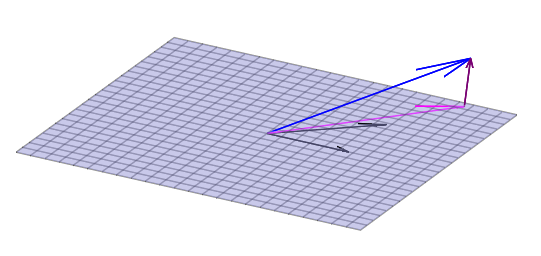
\includegraphics[width=0.5\linewidth]{images/lsqvec} 

}

\caption{A vector projection onto a subspace}\label{fig:oproj}
\end{figure}

Suppose we have a basis for \(\mathbb{R}^n\), like \(\{\mathbf{u}_1,\mathbf{u}_2,\dots,\mathbf{u}_n\}\). Then for any vector \(\mathbf{y}\) in \(\mathbb{R}^n\), we can write \(\mathbf{y}=\mathbf{z}_1+\mathbf{z}_2\), where \(\mathbf{z}_1\) is in the span of some of the \(\mathbf{u}_i\), while \(\mathbf{z}_2\) is what's left over. For example, suppose that \(\{\mathbf{u}_1,\mathbf{u}_2,\dots,\mathbf{u}_5\}\) is an orthogonal basis for \(\mathbb{R}^5\), and \(W\) is the subspace spanned by \(\mathbf{u}_1\) and \(\mathbf{u}_2\). Then

\[\mathbf{y}=\underbrace{c_1\mathbf{u}_1+c_2\mathbf{u}_2}_{\mathbf{z}_1}+\underbrace{c_3\mathbf{u}_3+c_4\mathbf{u}_4+c_5\mathbf{u}_5}_{\mathbf{z}_2}.\]

Note that \(\mathbf{z}_1\) is in the span of \(\mathbf{u}_1\) and \(\mathbf{u}_2\), so it is in \(W\). It should be clear that \(\mathbf{z}_2\) is in \(W^\perp\), since \(\mathbf{u}_3,\mathbf{u}_4,\) and \(\mathbf{u}_5\) are orthogonal to \(\mathbf{u}_1\) and \(\mathbf{u}_2\).

This decomposition of a vector into a sum of one vector from a subspace \(W\) and another one from \(W^\perp\) can always be done.

\begin{theorembox}

\begin{theorem}
Let \(W\) be a subspace of \(\mathbb{R}^n\). Then each \(\mathbf{y}\) in \(\mathbb{R}^n\) can be written uniquely in the form

\[\mathbf{y}=\hat{\mathbf{y}}+\mathbf{z},\]

where \(\hat{\mathbf{y}}\) is in \(W\) and \(\mathbf{z}\) is in \(W^\perp\). In fact, if \(\{\mathbf{u}_1,\dots \mathbf{u}_p\}\) is any orthogonal basis for \(W\), then

\[\hat{\mathbf{y}}=\frac{\mathbf{y}\cdot\mathbf{u}_1}{\mathbf{u}_1\cdot \mathbf{u}_1}\mathbf{u}_1+\cdots+\frac{\mathbf{y}\cdot \mathbf{u}_p}{\mathbf{u}_p\cdot \mathbf{u}_p}\mathbf{u}_p,\]

and \(\mathbf{z}=\mathbf{y}-\hat{\mathbf{y}}\).
\end{theorem}

\end{theorembox}

The vector \(\hat{\mathbf{y}}\) is the \emph{orthogonal projection}\index{Orthogonal!projection} of \(\mathbf{y}\) onto the subspace \(W\), denoted \(\text{proj}_W\mathbf{y}.\)

\begin{examplebox}

\begin{example}
Let

\[\mathbf{u}_1=\begin{bmatrix}3\\1\\1\end{bmatrix},\text{ and } \mathbf{u}_2=\begin{bmatrix}-1\\2\\1\end{bmatrix}.\]

If \(\mathbf{y}=(1,2,3)\), find the projection of \(\mathbf{y}\) onto the subspace \(W\) spanned by \(\mathbf{u}_1\) and \(\mathbf{u}_2\). (Note that \(\mathbf{u}_1\) and \(\mathbf{u}_2\) are orthogonal.) We have

\begin{align*} 
\hat{\mathbf{y}}&=\frac{\mathbf{y}\cdot\mathbf{u}_1}{\mathbf{u}_1\cdot \mathbf{u}_1}\mathbf{u}_1+\frac{\mathbf{y}\cdot\mathbf{u}_2}{\mathbf{u}_2\cdot \mathbf{u}_2}\mathbf{u}_2\\
&=\frac{8}{11}\begin{bmatrix}3\\1\\1\end{bmatrix}+\frac{6}{6}\begin{bmatrix}-1\\2\\1\end{bmatrix}=\begin{bmatrix}13/11\\30/11\\19/11\end{bmatrix}.
\end{align*}

We should see if \(\mathbf{z}=\mathbf{y}-\hat{\mathbf{y}}\) is in \(W^\perp\). We have

\[\mathbf{z}=\begin{bmatrix}1\\2\\3\end{bmatrix}-\begin{bmatrix}13/11\\30/11\\19/11\end{bmatrix}=\begin{bmatrix}-2/11\\-8/11\\14/11\end{bmatrix}.\]

Since

\[\mathbf{z}\cdot \mathbf{u}_1=\begin{bmatrix}-2/11\\-8/11\\14/11\end{bmatrix}\cdot\begin{bmatrix}3\\1\\1\end{bmatrix}=0,\text{ and }\mathbf{z}\cdot \mathbf{u}_2=\begin{bmatrix}-2/11\\-8/11\\14/11\end{bmatrix}\cdot\begin{bmatrix}-1\\2\\1\end{bmatrix}=0,\]

we see that \(\mathbf{z}\) is in \(W^\perp\).
\end{example}

\end{examplebox}

We mentioned in the last section that the projection of a vector \(\mathbf{y}\) onto a line spanned by another vector is the closest point on that line to \(\mathbf{y}\). The analogous result is true for projections onto more general subspaces.

\begin{theorembox}

\begin{theorem}
\protect\hypertarget{thm:lsp}{}\label{thm:lsp}Let \(W\) be a subspace of \(\mathbb{R}^n\), let \(\mathbf{y}\) be any vector in \(\mathbb{R}^n\), and let \(\hat{\mathbf{y}}\) be the orthogonal projection of \(\mathbf{y}\) onto \(W\). Then \(\hat{\mathbf{y}}\) is the closest point in \(W\) to \(\mathbf{y}\) in the sense that

\[|\mathbf{y}-\hat{\mathbf{y}}|< |\mathbf{y}-\mathbf{v}|\]

for all \(\mathbf{v}\) in \(W\) distinct from \(\hat{\mathbf{y}}\).
\end{theorem}

\end{theorembox}

\begin{proof}

We can write \(\mathbf{y}-\mathbf{v}=(\mathbf{y}-\hat{\mathbf{y}})+(\hat{\mathbf{y}}-\mathbf{v})\). Since \(\mathbf{v}\) is in \(W\), \(\hat{\mathbf{y}}-\mathbf{v}\) is too, and it is orthogonal to \(\mathbf{z}=\mathbf{y}-\hat{\mathbf{y}},\) so we can use the Pythagorean Theorem with \(\mathbf{y}-\mathbf{v}\) as the hypotenuse (see Fig. \ref{fig:yhat}):

\[|\mathbf{y}-\mathbf{v}|^2=|\mathbf{y}-\hat{\mathbf{y}}|^2+|\hat{\mathbf{y}}-\mathbf{v}|^2.\]

Since \(\hat{\mathbf{y}}\) and \(\mathbf{v}\) are distinct, \(|\hat{\mathbf{y}}-\mathbf{v}|^2>0\) and \(|\mathbf{y}-\mathbf{v}|^2>|\mathbf{y}-\hat{\mathbf{y}}|^2.\)

\begin{figure}

{\centering 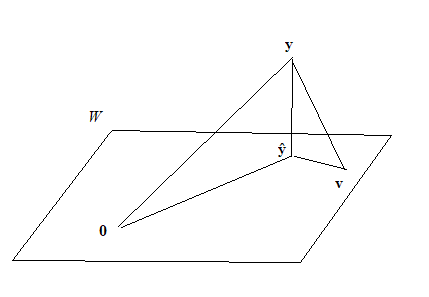
\includegraphics[width=0.6\linewidth]{images/yhat} 

}

\caption{Projection onto a subspace}\label{fig:yhat}
\end{figure}

\end{proof}

Things are again cleaner if we are working with an orthonormal basis.

\begin{theorembox}

\begin{theorem}
\protect\hypertarget{thm:Oproj}{}\label{thm:Oproj}If \(\{\mathbf{u}_1,\dots,\mathbf{u}_p\}\) is an orthonormal basis for a subspace \(W\) of \(\mathbb{R}^n\), then

\[\text{proj}_W\mathbf{y}=(\mathbf{y}\cdot\mathbf{u}_1)\mathbf{u}_1+\cdots+(\mathbf{y}\cdot\mathbf{u}_p)\mathbf{u}_p.\]

If \(\mathbf{U}=\begin{bmatrix}\mathbf{u}_1 & \mathbf{u}_2 & \cdots & \mathbf{u}_p\end{bmatrix}\), then

\[\text{proj}_W\mathbf{y}=\mathbf{U}\mathbf{U}^T\mathbf{y}\]

for all \(\mathbf{y}\) in \(\mathbb{R}^n\).
\end{theorem}

\end{theorembox}

The first part of this theorem is just the previous projection theorem with \(\mathbf{u}_i\cdot\mathbf{u}_i=1\) for all \(i\). The second part comes from the fact that the weights are \(\mathbf{u}_1^T\mathbf{y},\mathbf{u}_2^T\mathbf{y},\dots \mathbf{u}_p^T\mathbf{y}\) and can be written in a vector as \(\mathbf{U}^T\mathbf{y}\), which, when multiplied by \(\mathbf{U}\) on the left gives us the desired linear combination.

\begin{examplebox}

\begin{example}
Let \(W\) be the subspace of \(\mathbb{R}^3\) spanned by the orthonormal vectors

\[\{\mathbf{u}_1,\mathbf{u}_2\}=\left\{\begin{bmatrix}1/3\\2/3\\2/3\end{bmatrix},\begin{bmatrix} 2/3\\ 1/3\\-2/3\end{bmatrix}\right\}.\]

Find the projection matrix \(\mathbf{U}\mathbf{U}^T\) and use it to project the vector \(\mathbf{y}=(1,2,3)\) onto \(W\). With

\[\mathbf{U}=\begin{bmatrix} 1/3 & 2/3 \\ 2/3 & 1/3\\ 2/3 & -2/3\end{bmatrix},\]

we have

\[\mathbf{U}\mathbf{U}^T=\begin{bmatrix} 1/3 & 2/3 \\ 2/3 & 1/3\\ 2/3 & -2/3\end{bmatrix}\begin{bmatrix} 1/3 & 2/3 & 2/3\\2/3 & 1/3 & -2/3\end{bmatrix} =\begin{bmatrix} 5/9 & 4/9 & -2/9\\ 4/9 & 5/9 & 2/9\\ -2/9 & 2/9 & 8/9\end{bmatrix}.\]

(Remember that \(\mathbf{U}^T\mathbf{U}=\mathbf{I}\), the \(2\times 2\) identity matrix.) This gives us

\begin{align*}
\hat{\mathbf{y}}&=\mathbf{U}\mathbf{U}^T\mathbf{y}\\
&=\begin{bmatrix} 5/9 & 4/9 & -2/9\\ 4/9 & 5/9 & 2/9\\ -2/9 & 2/9 & 8/9\end{bmatrix}\begin{bmatrix}1\\2\\3\end{bmatrix}\\
&=\begin{bmatrix}7/9\\20/9\\26/9\end{bmatrix}.
\end{align*}

You can check to see that \(\mathbf{z}=\mathbf{y}-\hat{\mathbf{y}}=(2/9,-2/9,1/9)\) is orthogonal to \(\mathbf{u}_1\) and \(\mathbf{u}_2\).
\end{example}

\end{examplebox}

\section{Orthogonalization}\label{orthogonalization}

We don't always start out with an orthogonal basis for a subspace. There is a process for taking any basis and turning it into an orthogonal one, called the \emph{Gram-Schmidt}\index{Gram-Schmidt} process. Here's how we do it.

Suppose \(\{\mathbf{x}_1,\mathbf{x}_2,\dots,\mathbf{x}_p\}\) is a basis for a subspace \(W\) of \(\mathbb{R}^n\). Define

\begin{align}
    \mathbf{v}_1&=\mathbf{x}_1\\ \nonumber
    \mathbf{v}_2&=\mathbf{x}_2-\frac{\mathbf{x}_2\cdot \mathbf{v}_1}{\mathbf{v}_1\cdot\mathbf{v}_1}\mathbf{v}_1\\ \nonumber
    \mathbf{v}_3&=\mathbf{x}_3-\frac{\mathbf{x}_3\cdot \mathbf{v}_1}{\mathbf{v}_1\cdot\mathbf{v}_1}\mathbf{v}_1-\frac{\mathbf{x}_3\cdot \mathbf{v}_2}{\mathbf{v}_2\cdot \mathbf{v}_2}\mathbf{v}_2\\ \nonumber
    &\vdots\\ \nonumber
    \mathbf{v}_p&=\mathbf{x}_p-\frac{\mathbf{x}_p\cdot \mathbf{v}_1}{\mathbf{v}_1\cdot\mathbf{v}_1}\mathbf{v}_1-\frac{\mathbf{x}_p\cdot \mathbf{v}_2}{\mathbf{v}_2\cdot \mathbf{v}_2}\mathbf{v}_2-\cdots -\frac{\mathbf{x}_p\cdot \mathbf{v}_{p-1}}{\mathbf{v}_{p-1}\cdot \mathbf{v}_{p-1}}\mathbf{v}_{p-1}.
    \label{eq:gs}
\end{align}

Then \(\{\mathbf{v}_1,\mathbf{v}_2,\dots,\mathbf{v}_p\}\) is an orthogonal basis for \(W\). We can then get an orthonormal basis \(\{\mathbf{u}_1,\dots,\mathbf{u}_p\}\) for \(W\) with \(\mathbf{u}_i=\mathbf{v}_i/|\mathbf{v}_i|\) for \(i=1,\dots,p.\)

\textbf{How it works:} At each step, we're removing the part of the vector that is in the span of the previous ones, leaving us with a vector that is orthogonal to its predecessors. In practice, this can be tedious, and we can use technology to perform the process.
We will see a small example.

\begin{examplebox}

\begin{example}
\protect\hypertarget{exm:GS}{}\label{exm:GS}Let \(\mathbf{x}_1=\begin{bmatrix}1\\1\end{bmatrix}\) and let \(\mathbf{x}_2=\begin{bmatrix}1\\2\end{bmatrix}\). Note that \(\mathbf{x}_1\) and \(\mathbf{x}_2\) are linearly independent, so they span \(\mathbb{R}^2\). The first step is simple:

\[\mathbf{v}_1=\mathbf{x}_1=\begin{bmatrix}1\\1\end{bmatrix}.\]

Then

\begin{align*}
\mathbf{v}_2&=\mathbf{x}_2-\frac{\mathbf{x}_2\cdot \mathbf{v}_1}{\mathbf{v}_1\cdot\mathbf{v}_1}\mathbf{v}_1\\
&=\begin{bmatrix}1\\2\end{bmatrix}-\frac{(1,2)\cdot(1,1)}{(1,1)\cdot(1,1)}\begin{bmatrix}1\\1\end{bmatrix}\\
&=\begin{bmatrix}1\\2\end{bmatrix}-\frac{3}{2}\begin{bmatrix}1\\1\end{bmatrix}\\
&=\begin{bmatrix}-1/2\\1/2\end{bmatrix}.
\end{align*}

Now that we have an orthogonal basis, we can turn it into an orthonormal basis:

\[\{\mathbf{u}_1,\mathbf{u}_2\}=\left\{\frac{1}{|\mathbf{v}_1|}\mathbf{v}_1,\frac{1}{|\mathbf{v}_2|}\mathbf{v}_2\right\}.\]

With \(|\mathbf{v}_1|=\sqrt{1^2+1^2}=\sqrt{2}\) and
\(|\mathbf{v}_2|=\sqrt{(-1/2)^2+(1/2)^2}=\sqrt{1/2}=1/\sqrt{2}\), we have
\[\{\mathbf{u}_1,\mathbf{u}_2\}=\left\{\begin{bmatrix}1/\sqrt{2}\\1/\sqrt{2}\end{bmatrix},\begin{bmatrix}-1/\sqrt{2}\\1/\sqrt{2}\end{bmatrix}\right\}.\]
\end{example}

\end{examplebox}

\subsection*{QR-factorization}\label{qr-factorization}
\addcontentsline{toc}{subsection}{QR-factorization}

One bonus feature of the Gram-Schmidt orthonormalization procedure is that it leads to an important \emph{factorization} for certain matrices. Suppose that \(\mathbf{A}\) is an \(m\times n\) matrix with independent columns \(\{\mathbf{x}_1,\mathbf{x}_2,\dots,\mathbf{x}_n\}\) (so we must have \(n\leq m\)). By the Gram-Schmidt process, we can create an orthonormal collection of vectors using the columns of \(\mathbf{A}\), \(\{\mathbf{u}_1 ,\mathbf{u}_2 ,\dots , \mathbf{u}_n\}.\) Let \(\mathbf{Q}=\begin{bmatrix}\mathbf{u}_1 & \mathbf{u}_2 & \cdots & \mathbf{u}_n\end{bmatrix}\) be the \(m\times n\) matrix created using this orthonormal basis as the columns. For \(j=1\dots n,\mathbf{x}_j\) is in \(\text{span}(\mathbf{x}_1,\dots,\mathbf{x}_j)\), which is the same as \(\text{span}(\mathbf{u}_1,\cdots \mathbf{u}_j)\), so we can write

\[\mathbf{x}_j=r_{1j}\mathbf{u}_1+\cdots+r_{jj}\mathbf{u}_j+0\mathbf{u}_{j+1}+\cdots+0\mathbf{u}_n.\]

We can store these weights in the \(n\)-dimensional vector

\[\mathbf{r}_j=\begin{bmatrix}r_{1j}\\r_{2j}\\ \vdots \\r_{jj}\\0\\ \vdots\\0\end{bmatrix},\]

and \(\mathbf{x}_j=\mathbf{Q}\mathbf{r}_j\), for \(j=1\dots n\). If we define \(\mathbf{R}=\begin{bmatrix}\mathbf{r}_1 & \cdots & \mathbf{r}_n\end{bmatrix}\), then

\[\mathbf{A}=\begin{bmatrix}\mathbf{x}_1 & \cdots & \mathbf{x}_n\end{bmatrix}=\mathbf{Q}\mathbf{R}.\]

What we've just shown is that any \(m\times n\) matrix \(\mathbf{A}\) with linearly independent columns can be written as

\[\mathbf{A}=\mathbf{Q}\mathbf{R},\]

where \(\mathbf{Q}\) is an \(m\times n\) matrix with orthonormal columns that form a basis for the column space of \(\mathbf{A},\) and \(\mathbf{R}\) is an upper triangular matrix. This is the QR-factorization of \(\mathbf{A}.\)\index{QR-factorization}

Note that \(\mathbf{Q}\) comes from the Gram-Schmidt procedure, and we can calculate \(\mathbf{R}\) using the fact that

\[\mathbf{Q}^T\mathbf{A}=\mathbf{Q}^T\mathbf{Q}\mathbf{R}=\mathbf{I}\mathbf{R}=\mathbf{R},\]

so \(\mathbf{R}=\mathbf{Q}^T\mathbf{A}\).

\begin{examplebox}

\begin{example}
Let's use our work in Example \ref{exm:GS} to find a QR-factorization. Let

\[\mathbf{A}=\begin{bmatrix}1 & 1\\1 & 2\end{bmatrix},\]

the matrix whose columns are \(\mathbf{x}_1\) and \(\mathbf{x}_2\) from before. Our \(\mathbf{Q}\) matrix will be

\[\mathbf{Q}=\begin{bmatrix}1/\sqrt{2}&-1/\sqrt{2}\\1/\sqrt{2} & 1/\sqrt{2}\end{bmatrix}\]

and we can calculate \(\mathbf{R}:\)

\[\mathbf{R}=\mathbf{Q}^T\mathbf{A}=\begin{bmatrix}1/\sqrt{2} &1/\sqrt{2}\\-1/\sqrt{2} & 1/\sqrt{2}\end{bmatrix}\begin{bmatrix}1 & 1\\1 & 2\end{bmatrix}=\begin{bmatrix}\sqrt{2} & 3/\sqrt{2}\\0 & 1/\sqrt{2}\end{bmatrix}.\]

Lets check:

\[\mathbf{Q}\mathbf{R}=\begin{bmatrix}1/\sqrt{2}&-1/\sqrt{2}\\1/\sqrt{2} & 1/\sqrt{2}\end{bmatrix}\begin{bmatrix}\sqrt{2} & 3/\sqrt{2}\\0 & 1/\sqrt{2}\end{bmatrix}=\begin{bmatrix}1 & 1\\1 & 2\end{bmatrix}\checkmark.\]
\end{example}

\end{examplebox}

Why is this factorization useful? Suppose we are trying to solve \(\mathbf{A}\mathbf{x}=\mathbf{y}\), and we have the QR-factorization for \(\mathbf{A}\). Then

\begin{align*}
\mathbf{A}\mathbf{x}&=\mathbf{y}\\
\mathbf{Q}\mathbf{R}\mathbf{x}&=\mathbf{y}\\
\mathbf{Q}^T\mathbf{Q}\mathbf{R}\mathbf{x}&=\mathbf{Q}^T\mathbf{y}\\
\mathbf{R}\mathbf{x}&=\mathbf{Q}^T\mathbf{y}
\end{align*}

Finding a matrix inverse, especially for a large matrix, can be numerically challenging. Since \(\mathbf{Q}\) is orthogonal, its inverse is just its transpose, which is a simple computational task. Since \(\mathbf{R}\) is upper triangular, we can solve the remaining problem by back substitution, which is also fairly computationally easy.

The R package \texttt{pracma} has a \texttt{gramSchmidt} function that will find the QR-factorization of a matrix. The columns of \(\mathbf{Q}\) will have the Gram-Schmidt orthonormal basis for the column space of the original matrix.

\begin{Shaded}
\begin{Highlighting}[]
\FunctionTok{library}\NormalTok{(pracma)}
\NormalTok{A }\OtherTok{\textless{}{-}} \FunctionTok{matrix}\NormalTok{(}\FunctionTok{c}\NormalTok{(}\DecValTok{1}\NormalTok{,}\DecValTok{2}\NormalTok{,}\DecValTok{3}\NormalTok{,}\DecValTok{4}\NormalTok{,}\DecValTok{5}\NormalTok{,}\DecValTok{6}\NormalTok{), }\AttributeTok{nrow =} \DecValTok{3}\NormalTok{)}
\NormalTok{A}
\end{Highlighting}
\end{Shaded}

\begin{verbatim}
##      [,1] [,2]
## [1,]    1    4
## [2,]    2    5
## [3,]    3    6
\end{verbatim}

\begin{Shaded}
\begin{Highlighting}[]
\FunctionTok{gramSchmidt}\NormalTok{(A)}
\end{Highlighting}
\end{Shaded}

\begin{verbatim}
## $Q
##           [,1]       [,2]
## [1,] 0.2672612  0.8728716
## [2,] 0.5345225  0.2182179
## [3,] 0.8017837 -0.4364358
## 
## $R
##          [,1]     [,2]
## [1,] 3.741657 8.552360
## [2,] 0.000000 1.963961
\end{verbatim}

If the columns of the matrix are dependent, we will get an error.

\begin{Shaded}
\begin{Highlighting}[]
\NormalTok{B }\OtherTok{\textless{}{-}} \FunctionTok{matrix}\NormalTok{(}\FunctionTok{c}\NormalTok{(}\DecValTok{1}\NormalTok{,}\DecValTok{2}\NormalTok{,}\DecValTok{3}\NormalTok{,}\DecValTok{2}\NormalTok{,}\DecValTok{4}\NormalTok{,}\DecValTok{6}\NormalTok{), }\AttributeTok{nrow =} \DecValTok{3}\NormalTok{)}
\NormalTok{B}
\end{Highlighting}
\end{Shaded}

\begin{verbatim}
##      [,1] [,2]
## [1,]    1    2
## [2,]    2    4
## [3,]    3    6
\end{verbatim}

\begin{Shaded}
\begin{Highlighting}[]
\FunctionTok{gramSchmidt}\NormalTok{(B)}
\end{Highlighting}
\end{Shaded}

\begin{verbatim}
## Error in gramSchmidt(B): Matrix 'A' does not have full rank.
\end{verbatim}

\section{Exercises}\label{exercises-3}

\begin{enumerate}
\def\labelenumi{\arabic{enumi}.}
\item
  Let \(\mathbf{v}=\begin{bmatrix}1\\5\\-2\end{bmatrix}.\)

  \begin{enumerate}
  \def\labelenumii{\alph{enumii}.}
  \tightlist
  \item
    Find a unit vector in the direction of \(\mathbf{v}\).
  \item
    Find two independent vectors that are orthogonal to \(\mathbf{v}.\)
  \end{enumerate}
\item
  Let \(\mathbf{v}=\begin{bmatrix}1\\-4\\6\end{bmatrix}.\)

  \begin{enumerate}
  \def\labelenumii{\alph{enumii}.}
  \tightlist
  \item
    Find a unit vector in the direction of \(\mathbf{v}\).
  \item
    Find two independent vectors that are orthogonal to \(\mathbf{v}.\)
  \end{enumerate}
\item
  Let \(\mathbf{a}_1=\begin{bmatrix}1\\3\\4\end{bmatrix}\) and \(\mathbf{a}_2=\begin{bmatrix} 2\\2\\-2\end{bmatrix}.\)

  \begin{enumerate}
  \def\labelenumii{\alph{enumii}.}
  \tightlist
  \item
    Show that \(\mathbf{a}_1\) and \(\mathbf{a}_2\) are orthogonal.
  \item
    Find a third nonzero vector \(\mathbf{a}_3\) that is orthogonal to both \(\mathbf{a}_1\) and \(\mathbf{a}_2.\) Use the following method: let \(\mathbf{a}_1\) and \(\mathbf{a}_2\) be the rows of a matrix. A vector orthogonal to the rows would be in what space?
  \end{enumerate}
\item
  Let \(\mathbf{a}_1=\begin{bmatrix}1\\2\\6\end{bmatrix}\) and \(\mathbf{a}_2=\begin{bmatrix} 2\\2\\-1\end{bmatrix}.\)

  \begin{enumerate}
  \def\labelenumii{\alph{enumii}.}
  \tightlist
  \item
    Show that \(\mathbf{a}_1\) and \(\mathbf{a}_2\) are orthogonal.
  \item
    Find a third nonzero vector \(\mathbf{a}_3\) that is orthogonal to both \(\mathbf{a}_1\) and \(\mathbf{a}_2.\)
  \end{enumerate}
\item
  Let \(\mathbf{v}_1=\begin{bmatrix}1\\1\\1\end{bmatrix},\mathbf{v}_2=\begin{bmatrix} 3\\1\\-4\end{bmatrix},\) and \(\mathbf{v}_3=\begin{bmatrix}5\\-7\\2\end{bmatrix}.\)

  \begin{enumerate}
  \def\labelenumii{\alph{enumii}.}
  \tightlist
  \item
    Show that \(\{\mathbf{v}_1,\mathbf{v}_2,\mathbf{v}_3\}\) is an orthogonal set.
  \item
    Write \(\mathbf{y}=\begin{bmatrix} 2\\3\\4\end{bmatrix}\) as a linear combination of \(\mathbf{v}_1,\mathbf{v}_2,\) and \(\mathbf{v}_3.\)
  \end{enumerate}
\item
  Let \(\mathbf{v}_1=\begin{bmatrix}1\\2\\1\end{bmatrix},\mathbf{v}_2=\begin{bmatrix} 2\\0\\-2\end{bmatrix},\) and \(\mathbf{v}_3=\begin{bmatrix}1\\-1\\1\end{bmatrix}.\)

  \begin{enumerate}
  \def\labelenumii{\alph{enumii}.}
  \tightlist
  \item
    Show that \(\{\mathbf{v}_1,\mathbf{v}_2,\mathbf{v}_3\}\) is an orthogonal set.
  \item
    Write \(\mathbf{y}=\begin{bmatrix} 4\\3\\2\end{bmatrix}\) as a linear combination of \(\mathbf{v}_1,\mathbf{v}_2,\) and \(\mathbf{v}_3.\)
  \end{enumerate}
\item
  Let \(\mathbf{u}=\begin{bmatrix}1\\2\\-3\end{bmatrix}\) and \(\mathbf{y}=\begin{bmatrix}1\\2\\3\end{bmatrix}.\)

  \begin{enumerate}
  \def\labelenumii{\alph{enumii}.}
  \tightlist
  \item
    Find \(\hat{\mathbf{y}}=\text{proj}_\mathbf{u}\mathbf{y}.\)
  \item
    Show that \(\mathbf{z}=\mathbf{y}-\hat{\mathbf{y}}\) is orthogonal to \(\mathbf{u}.\)
  \end{enumerate}
\item
  Let \(\mathbf{u}=\begin{bmatrix}6\\0\\8\end{bmatrix}\) and \(\mathbf{y}=\begin{bmatrix}2\\1\\0\end{bmatrix}.\)

  \begin{enumerate}
  \def\labelenumii{\alph{enumii}.}
  \tightlist
  \item
    Find \(\hat{\mathbf{y}}=\text{proj}_\mathbf{u}\mathbf{y}.\)
  \item
    Show that \(\mathbf{z}=\mathbf{y}-\hat{\mathbf{y}}\) is orthogonal to \(\mathbf{u}.\)
  \end{enumerate}
\item
  Turn \(\{\mathbf{v}_1,\mathbf{v}_2,\mathbf{v}_3\}\) from Problem 5 into an orthonormal set.
\item
  Turn \(\{\mathbf{v}_1,\mathbf{v}_2,\mathbf{v}_3\}\) from Problem 6 into an orthonormal set.
\item
  Let \(W\) be the subspace of \(\mathbb{R}^3\) spanned by the orthonormal vectors
  \[\{\mathbf{u}_1,\mathbf{u}_2\}=\left\{\begin{bmatrix}3/7\\6/7\\-2/7\end{bmatrix},\begin{bmatrix}-2/7\\3/7\\6/7\end{bmatrix}\right\}.\]

  \begin{enumerate}
  \def\labelenumii{\alph{enumii}.}
  \tightlist
  \item
    Let \(\mathbf{U}=\begin{bmatrix} \mathbf{u}_1 & \mathbf{u}_2\end{bmatrix}.\) Find the projection matrix \(\mathbf{U}\mathbf{U}^T.\)
  \item
    Project \(\mathbf{y}=\begin{bmatrix}1\\1\\1\end{bmatrix}\) onto the subspace spanned by \(\mathbf{u}_1\) and \(\mathbf{u}_2.\)
  \end{enumerate}
\item
  Let \(W\) be the subspace of \(\mathbb{R}^3\) spanned by the orthonormal vectors
  \[\{\mathbf{u}_1,\mathbf{u}_2\}=\left\{\begin{bmatrix}3/13\\12/13\\-4/13\end{bmatrix},\begin{bmatrix}4/13\\3/13\\12/13\end{bmatrix}\right\}.\]

  \begin{enumerate}
  \def\labelenumii{\alph{enumii}.}
  \tightlist
  \item
    Let \(\mathbf{U}=\begin{bmatrix} \mathbf{u}_1 & \mathbf{u}_2\end{bmatrix}.\) Find the projection matrix \(\mathbf{U}\mathbf{U}^T.\)
  \item
    Project \(\mathbf{y}=\begin{bmatrix}1\\1\\1\end{bmatrix}\) onto the subspace spanned by \(\mathbf{u}_1\) and \(\mathbf{u}_2.\)
  \end{enumerate}
\item
  Let
  \[\mathbf{A}=\begin{bmatrix}1 & 1 & 0\\1 & 1 & 1\\0 & 1 & 1\end{bmatrix}.\]

  \begin{enumerate}
  \def\labelenumii{\alph{enumii}.}
  \tightlist
  \item
    Perform the Gram-Schmidt orthonormalization procedure on the columns of \(\mathbf{A}\) by hand.
  \item
    Find the QR-factorization of \(\mathbf{A}\)
  \end{enumerate}
\item
  Let
  \[\mathbf{A}=\begin{bmatrix}0 & 1 & 1\\1 & 1 & 1\\1 & 1 & 0\end{bmatrix}.\]

  \begin{enumerate}
  \def\labelenumii{\alph{enumii}.}
  \tightlist
  \item
    Perform the Gram-Schmidt orthonormalization procedure on the columns of \(\mathbf{A}\) by hand.
  \item
    Find the QR-factorization of \(\mathbf{A}\)
  \end{enumerate}
\item
  Use the Gram-Schmidt procedure to find a third vector that is orthogonal to the two vectors given in Problem 3. Hint: \(\mathbf{e}_1,\) the first standard basis vector is not in the span of \(\mathbf{a}_1\) and \(\mathbf{a}_2\).
\item
  Use the Gram-Schmidt procedure to find a third vector that is orthogonal to the two vectors given in Problem 4. Hint: \(\mathbf{e}_1,\) the first standard basis vector is not in the span of \(\mathbf{a}_1\) and \(\mathbf{a}_2\).
\end{enumerate}

\chapter{Regression}\label{regression}

The focus in this chapter is regression: fitting linear and similar models to data. There is a beautiful connection between this problem and the matrix algebra material that we have studied so far.

\section{Least Squares Problems}\label{LSQP}

Some linear equations have no solution. For instance, if we try to solve \(\mathbf{A}\mathbf{x}=\mathbf{b}\), where

\[\mathbf{A}=\begin{bmatrix}4 & 0\\0 & 2\\ 1& 1\end{bmatrix}, \text{ and } \mathbf{b}=\begin{bmatrix}2\\0\\11\end{bmatrix},\]

we run into a problem when we put the augmented matrix in reduced row echelon form:

\[\left[\begin{array}{cc|c}4 & 0 & 2\\0 & 2 & 0\\1 & 1 & 11\end{array}\right]\leadsto \left[\begin{array}{cc|c} 1 & 0 & 0\\0 & 1 & 0\\0 & 0 & 1\end{array}\right].\]

Remember that the last row says \(0=1\), so there is no solution. In terms of linear algebra, what is going on here? The matrix product

\[\mathbf{A}\mathbf{x}=\begin{bmatrix}4 & 0\\0 & 2\\ 1& 1\end{bmatrix}\begin{bmatrix}x_1\\x_2\end{bmatrix}=\begin{bmatrix}4x_1+0x_2\\0x_1+2x_2\\1x_1+1x_2\end{bmatrix}=x_1\begin{bmatrix}4\\0\\1\end{bmatrix}+x_2\begin{bmatrix}0\\2\\1\end{bmatrix}\]

is really a linear combination of the columns of \(\mathbf{A}.\) There is no solution because

\[\mathbf{b}=\begin{bmatrix}2\\0\\11\end{bmatrix}\]

cannot be written as a linear combination of the columns of \(\mathbf{A}.\) That is, \(\mathbf{b}\) is not in the column space of \(\mathbf{A}.\)

In a \emph{least squares problem}\index{Least squares problem}, we project \(\mathbf{b}\) into the column space of \(\mathbf{A}\) (see Fig. \ref{fig:oproj2})

\[\hat{\mathbf{b}}=\text{proj}_{\text{Col}(\mathbf{A})}\mathbf{b},\]

and solve \(\mathbf{A}\mathbf{x}=\hat{\mathbf{b}}\), which we know will have a solution.

\begin{figure}

{\centering 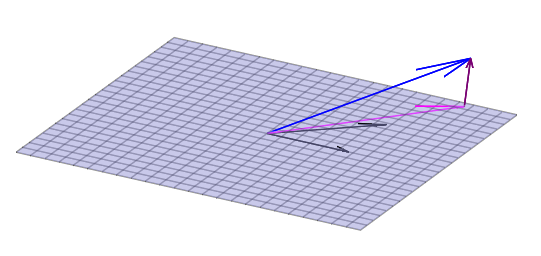
\includegraphics[width=0.75\linewidth]{images/lsqvec} 

}

\caption{A projection onto the column space}\label{fig:oproj2}
\end{figure}

Why do we call it ``least squares?'' Remember from Theorem \ref{thm:lsp} that the projection \(\hat{\mathbf{b}}\) satisfies

\[|\mathbf{b}-\hat{\mathbf{b}}|<|\mathbf{b}-\mathbf{v}|\]

for any vector \(\mathbf{v}\) in \(\text{Col}(\mathbf{A})\) different from \(\hat{\mathbf{b}}\). If \(\mathbf{b}=(b_1,b_2,b_3)\) and \(\mathbf{v}=(v_1,v_2,v_3),\) then

\[|\mathbf{b}-\mathbf{v}|^2=(b_1-v_1)^2+(b_2-v_2)^2+(b_3-v_3)^2.\]

The projection \(\hat{\mathbf{b}}\) minimizes this sum of squares over all possible vectors in \(\text{Col}(\mathbf{A})\).

How do we find the least squares solution? We want to find a vector \(\hat{\mathbf{x}}\) that satisfies

\[\mathbf{A}\hat{\mathbf{x}}=\hat{\mathbf{b}}.\]

The key is that \(\mathbf{b}-\hat{\mathbf{b}}\) is orthogonal to the column space of \(\mathbf{A}.\) If \(\mathbf{a}_j\) is any column of \(\mathbf{A},\) then \(\mathbf{a}_j\cdot(\mathbf{b}-\hat{\mathbf{b}})=0\), or

\[\mathbf{a}_j^T (\mathbf{b}-\hat{\mathbf{b}})=\mathbf{a}_j^T (\mathbf{b}-\mathbf{A}\hat{\mathbf{x}})=0.\]

Since the \(\mathbf{a}_j^T\) vectors form the rows of \(\mathbf{A}^T\) we actually have

\[\mathbf{A}^T(\mathbf{b}-\mathbf{A}\hat{\mathbf{x}})=\mathbf{0}.\]

When we apply the distributive law to

\[\mathbf{A}^T(\mathbf{b}-\mathbf{A}\hat{\mathbf{x}})=\mathbf{0},\]

we get

\[\mathbf{A}^T\mathbf{b}-\mathbf{A}^T\mathbf{A}\hat{\mathbf{x}}=\mathbf{0},\]

or

\[\mathbf{A}^T\mathbf{A}\hat{\mathbf{x}}=\mathbf{A}^T\mathbf{b}.\]

This leads us to what are called the \emph{normal equations}\index{Normal equations}.

\begin{theorembox}

\begin{theorem}
\protect\hypertarget{thm:NormalEq}{}\label{thm:NormalEq}The set of least-squares solutions of \(\mathbf{A}\mathbf{x}=\mathbf{b}\) coincides with the nonempty set of solutions of the normal equations

\[\mathbf{A}^T\mathbf{A}\hat{\mathbf{x}}=\mathbf{A}^T\mathbf{b}.\]
\end{theorem}

\end{theorembox}

By the nature of the problem, there will always be a least-squares solution for the equation \(\mathbf{A}\mathbf{x}=\mathbf{b}\). Under additional conditions, the solution will be unique. We'll see those conditions in a bit.

\begin{examplebox}

\begin{example}
\protect\hypertarget{exm:ls1}{}\label{exm:ls1}Let's return to our example

\[\begin{bmatrix}4 & 0\\0 & 2\\ 1& 1\end{bmatrix}\mathbf{x}=\begin{bmatrix}2\\0\\11\end{bmatrix}\]

and find a least squares solution. We calculate

\[\mathbf{A}^T\mathbf{A}=\begin{bmatrix}4 & 0 & 1\\0 & 2 & 1\end{bmatrix}\begin{bmatrix}4 & 0\\0 & 2\\ 1& 1\end{bmatrix}=\begin{bmatrix}17 & 1\\1 & 5\end{bmatrix}\]

and

\[\mathbf{A}^T\mathbf{b}=\begin{bmatrix}4 & 0 & 1\\0 & 2 & 1\end{bmatrix}\begin{bmatrix}2\\0\\11\end{bmatrix}=\begin{bmatrix}19\\11\end{bmatrix}.\]

To find our least squares solution, we solve
\(\mathbf{A}^T\mathbf{A}\hat{\mathbf{x}}=\mathbf{A}^T\mathbf{b}\):

\[\begin{bmatrix}17 & 1\\1 & 5\end{bmatrix}\hat{\mathbf{x}}=\begin{bmatrix}19\\11\end{bmatrix}.\]

Using the inverse of \(\mathbf{A}^T\mathbf{A}\), we get our solution:

\[\hat{\mathbf{x}}=\frac{1}{17\cdot 5-1\cdot 1}\begin{bmatrix}5 & -1\\-1 & 17\end{bmatrix}\begin{bmatrix}19\\11\end{bmatrix}=\frac{1}{84}\begin{bmatrix}84\\168\end{bmatrix}=\begin{bmatrix}1\\2\end{bmatrix}.\]
\end{example}

\end{examplebox}

\begin{examplebox}

\begin{example}
\protect\hypertarget{exm:ims}{}\label{exm:ims}Find the least squares solution to

\[\begin{bmatrix}1 & 1 & 0 & 0\\1 & 1 & 0 & 0\\1 & 0 & 1 & 0\\1 & 0 & 1 & 0\\1 & 0 & 0 & 1\\1 & 0 & 0 & 1\end{bmatrix}\mathbf{x}=\begin{bmatrix}-3\\-1\\0\\2\\5\\1\end{bmatrix}.\]

Note that the first column is the sum of the other three, so the columns are linearly dependent.

If we try to find a regular (non-least squares) solution to the equation via row reduction, we get

\[\left[\begin{array}{cccc|r} 1 & 1 & 0 & 0 & -3\\1 & 1 & 0 & 0 & -1\\1 & 0 & 1 & 0 & 0\\ 1 & 0 & 1 & 0 & 2\\1 & 0 & 0 & 1 & 5\\1 & 0 & 0 & 1 & 1\end{array}\right]\leadsto \left[\begin{array}{cccr|r} 1 & 0 & 0 & 1 & 0\\0 & 1 & 0 & -1 & 0\\0 & 0 & 1 & -1 & 0\\0 & 0 & 0 & 0 & 1\\0 & 0 & 0 & 0 & 0 \\0 & 0 & 0 & 0 & 0\end{array}\right],\]

so there is no solution. For the normal equations, we find

\[\mathbf{A}^T\mathbf{A}=\begin{bmatrix}1 & 1 & 1 & 1 & 1 & 1\\1 & 1 & 0 & 0 & 0 & 0\\0 & 0 & 1 & 1 & 0 & 0\\0 & 0 & 0 & 0 & 1 & 1\end{bmatrix}\begin{bmatrix}1 & 1 & 0 & 0\\1 & 1 & 0 & 0\\1 & 0 & 1 & 0\\1 & 0 & 1 & 0\\1 & 0 & 0 & 1\\1 & 0 & 0 & 1\end{bmatrix}=\begin{bmatrix}6 & 2 & 2 & 2\\2 & 2 & 0 & 0\\2 & 0 & 2 & 0\\2 & 0 & 0 & 2\end{bmatrix},\]

and

\[\mathbf{A}^T\mathbf{b}=\begin{bmatrix}1 & 1 & 1 & 1 & 1 & 1\\1 & 1 & 0 & 0 & 0 & 0\\0 & 0 & 1 & 1 & 0 & 0\\0 & 0 & 0 & 0 & 1 & 1\end{bmatrix}\begin{bmatrix}-3\\-1\\0\\2\\5\\1\end{bmatrix}=\begin{bmatrix}4\\-4\\2\\6\end{bmatrix}.\]

It turns out that \(\mathbf{A}^T\mathbf{A}\) is not invertible, so we use row reduction to solve:

\[\left[\begin{array}{cccc|r} 6 & 2 & 2 & 2 & 4\\2 & 2 & 0 & 0& -4\\2 & 0 & 2 & 0 & 2\\2 & 0 & 0 & 2& 6\end{array}\right] \leadsto \left[\begin{array}{cccr|r}1 & 0 & 0 & 1 & 3\\0 & 1 & 0 & -1 & -5\\0 & 0 & 1 & -1 & -2\\0 & 0 & 0 & 0 & 0\end{array}\right].\]

With \(x_4=t\) as a free variable, we have \(x_1=3-t,x_2=-5+t\), and \(x_3=-2+t\). We can write our least squares solution as

\[\hat{\mathbf{x}}=\begin{bmatrix}3\\-5\\-2\\0\end{bmatrix}+t\begin{bmatrix}-1\\1\\1\\1\end{bmatrix}.\]

Note that the vector multiplied by \(t\) is in the null space of \(\mathbf{A}^T\mathbf{A}\) and the null space of \(\mathbf{A},\) too. They actually share the same null space.
\end{example}

\end{examplebox}

\begin{theorembox}

\begin{theorem}
Let \(\mathbf{A}\) be an \(m\times n\) matrix. Then \(\mathbf{A}\) and \(\mathbf{A}^T\mathbf{A}\) have the same nullspace.
\end{theorem}

\end{theorembox}

\begin{proof}
Let \(\mathbf{x}\in \text{Null}(\mathbf{A})\). Then

\[ (\mathbf{A}^T\mathbf{A})\mathbf{x}=\mathbf{A}^T(\mathbf{A}\mathbf{x})=\mathbf{A}^T\mathbf{0}=\mathbf{0}.\]

Any vector in the nullspace of \(\mathbf{A}\) is also in the nullspace of \(\mathbf{A}^T\mathbf{A}\). Suppose \(\mathbf{x}\in\text{Null}(\mathbf{A}^T\mathbf{A}).\) Then

\[\mathbf{A}^T(\mathbf{A}\mathbf{x})=(\mathbf{A}^T\mathbf{A})\mathbf{x}=\mathbf{0}.\]

That means that \(\mathbf{x}\in \text{Null}(\mathbf{A}^T).\) From Theorem \ref{thm:MatSubspaces} (see, we're using it), we know that \(\text{Null}(\mathbf{A}^T)=\text{Col}(\mathbf{A})^{\perp}.\) The vector \(\mathbf{A}\mathbf{x}\) is simultaneously in \(\text{Col}(\mathbf{A})^{\perp}\) and \(\text{Col}(\mathbf{A})\). The only vector common to a subspace and its orthogonal complement is the zero vector, so \(\mathbf{A}\mathbf{x}=\mathbf{0}\) and \(\mathbf{x}\in\text{Null}(\mathbf{A}).\) Any vector in \(\text{Null}(\mathbf{A}^T\mathbf{A})\) is also in \(\text{Null}(\mathbf{A}).\) They are the same subspace.
\end{proof}

Why did Example \ref{exm:ims} have infinitely many solutions? Since the columns of \(\mathbf{A}\) were not linearly independent, there were actually infinitely many ways to write the projection \(\hat{\mathbf{b}}\) in terms of them. This does not happen when the columns are linearly independent.

\begin{theorembox}

\begin{theorem}
Let \(\mathbf{A}\) be an \(m\times n\) matrix. The following are equivalent:

\begin{enumerate}
\def\labelenumi{\arabic{enumi}.}
\item
  The equation \(\mathbf{A}\mathbf{x}=\mathbf{b}\) has a unique least squares solution for each \(\mathbf{b}\) in \(\mathbb{R}^m\).
\item
  The columns of \(\mathbf{A}\) are linearly independent.
\item
  The matrix \(\mathbf{A}^T\mathbf{A}\) is invertible.
\end{enumerate}

When these statements are true, the least squares solution is given by

\[\hat{\mathbf{x}}=(\mathbf{A}^T\mathbf{A})^{-1}\mathbf{A}^T\mathbf{b}.\]
\end{theorem}

\end{theorembox}

The last formula

\[\hat{\mathbf{x}}=(\mathbf{A}^T\mathbf{A})^{-1}\mathbf{A}^T\mathbf{b}\]

looks awkward, and we might be tempted to use the formula for the inverse of a product

\[(\mathbf{A}\mathbf{B})^{-1}=\mathbf{B}^{-1}\mathbf{A}^{-1},\]
but there are two issues:

\begin{enumerate}
\def\labelenumi{\arabic{enumi}.}
\item
  \(\mathbf{A}\) and \(\mathbf{A}^T\) are not necessarily invertible and,
\item
  They don't even need to be square.
\end{enumerate}

In fact, if \(\mathbf{A}\) were invertible, then we wouldn't need a least squares solution, since \(\mathbf{x}=\mathbf{A}^{-1}\mathbf{b}\) is a regular solution.

\subsection*{Least squares error}\label{least-squares-error}
\addcontentsline{toc}{subsection}{Least squares error}

How close does the least squares solution come to being an actual solution? The distance between \(\mathbf{b}\) and \(\hat{\mathbf{b}}\), which is \(|\mathbf{b}-\hat{\mathbf{b}}|=|\mathbf{b}-\mathbf{A}\hat{\mathbf{x}}|\), tells us this.

In Example \ref{exm:ls1},

\[\mathbf{b}=\begin{bmatrix}2\\0\\11\end{bmatrix},\]

while

\[\hat{\mathbf{b}}=\mathbf{A}\hat{\mathbf{x}}=\begin{bmatrix}4&0\\0 & 2\\1 & 1\end{bmatrix}\begin{bmatrix}1\\2\end{bmatrix}=\begin{bmatrix}4\\4\\3\end{bmatrix}.\]

The least squares error\index{Least squares error} is

\[\sqrt{(2-4)^2+(0-4)^2+(11-3)^2}=\sqrt{84}\approx 9.2.\]

\subsection*{Least squares and the QR-factorization}\label{least-squares-and-the-qr-factorization}
\addcontentsline{toc}{subsection}{Least squares and the QR-factorization}

If the columns of \(\mathbf{A}\) are linearly independent, then we can write \(\mathbf{A}=\mathbf{Q}\mathbf{R}\), where \(\mathbf{Q}\) is orthogonal and \(\mathbf{R}\) is invertible. In this case, the least squares solution is given by

\[\hat{\mathbf{x}}=\mathbf{R}^{-1}\mathbf{Q}^T\mathbf{b}.\]

Why does this work? If \(\hat{\mathbf{x}}=\mathbf{R}^{-1}\mathbf{Q}^T\mathbf{b}\), then

\[\mathbf{A}\hat{\mathbf{x}}=\mathbf{Q}\mathbf{R}\hat{\mathbf{x}}=\mathbf{Q}\mathbf{R}\mathbf{R}^{-1}\mathbf{Q}^T\mathbf{b}=\mathbf{Q}\mathbf{Q}^T\mathbf{b},\]

which we learned in Theorem \ref{thm:Oproj} is the orthogonal projection of \(\mathbf{b}\) onto the column space of \(\mathbf{Q}\), which is the same as the column space of \(\mathbf{A}\). This projection is \(\hat{\mathbf{b}}\).

\section{Application: The Massey Method}\label{application-the-massey-method}

So far, all of our ranking methods have ignored the points scored by teams or players. The \emph{Massey Method}\index{Massey method} is a least squares method that is actually designed to predict the point spread in a competition. Ken Massey developed his method as part of an honors project in college \autocite{Massey}. His site \href{http://masseyratings.com}{masseyratings.com} is also an excellent source of sports schedule data.

The development and notation in this section come from Amy Langville and Carl Meyer \autocite{No1}. The idea behind the ratings is that if teams \(i\) and \(j\) play in game number \(k\), the point spread \(y_k\) will just be the difference of the two teams ratings:

\[r_i-r_j=y_k.\]

Note that this method can easily handle ties, since we can just set the margin of victory to be 0. If there are \(n\) teams in the league, and a total of \(m\) games, we will get an \(m\times n\) system of equations. Since the number of games will quickly exceed the number of teams, the system of equations will be overdetermined, but we can still find a least squares solution.

Recall our toy example.

\begin{longtable}[]{@{}
  >{\raggedright\arraybackslash}p{(\columnwidth - 10\tabcolsep) * \real{0.1795}}
  >{\raggedleft\arraybackslash}p{(\columnwidth - 10\tabcolsep) * \real{0.1923}}
  >{\raggedleft\arraybackslash}p{(\columnwidth - 10\tabcolsep) * \real{0.1667}}
  >{\raggedleft\arraybackslash}p{(\columnwidth - 10\tabcolsep) * \real{0.1410}}
  >{\raggedleft\arraybackslash}p{(\columnwidth - 10\tabcolsep) * \real{0.1667}}
  >{\raggedleft\arraybackslash}p{(\columnwidth - 10\tabcolsep) * \real{0.1538}}@{}}
\toprule\noalign{}
\begin{minipage}[b]{\linewidth}\raggedright
\end{minipage} & \begin{minipage}[b]{\linewidth}\raggedleft
\textbf{Aardvarks}
\end{minipage} & \begin{minipage}[b]{\linewidth}\raggedleft
\textbf{Beagles}
\end{minipage} & \begin{minipage}[b]{\linewidth}\raggedleft
\textbf{Crocs}
\end{minipage} & \begin{minipage}[b]{\linewidth}\raggedleft
\textbf{Donkeys}
\end{minipage} & \begin{minipage}[b]{\linewidth}\raggedleft
\textbf{Egrets}
\end{minipage} \\
\midrule\noalign{}
\endhead
\bottomrule\noalign{}
\endlastfoot
\textbf{Aardvarks} & x & 17-31 & 6-42 & x & 17-7 \\
\textbf{Beagles} & & x & 3-59 & 10-35 & x \\
\textbf{Crocs} & & & x & 21-20 & 49-0 \\
\textbf{Donkeys} & & & & x & 28-21 \\
\textbf{Egrets} & & & & & x \\
\end{longtable}

The first few lines of the system of equations will look like this

\[ \left\{\begin{array}{rrr}
    r_1-r_2&=&-14\\
    r_1-r_3&=&-36\\
    r_1-r_5&=&10
\end{array} \right. .
\]

In matrix form, the full system looks like this.

\[\left[\begin{array}{rrrrr}1 & -1 & 0 & 0 & 0\\1 & 0 & -1 & 0 & 0\\1 & 0 & 0 & 0 & -1\\0 & 1 & -1 & 0 & 0\\0 & 1 & 0 & -1 & 0\\0 & 0 & 1 & -1 & 0 \\0 & 0 & 1 & 0 & -1\\0 & 0 & 0 & 1 & -1\end{array}\right]\begin{bmatrix}r_1\\r_2\\r_3\\r_4\\r_5\end{bmatrix}=\left[\begin{array}{r}-14 \\-36\\10\\-56\\-25\\1\\49\\7\end{array}\right]\]

or

\[\mathbf{X}\mathbf{r}=\mathbf{y}.\]

This system is overdetermined, so we instead solve the normal equations

\[\mathbf{X}^T\mathbf{X}\mathbf{r}=\mathbf{X}^T\mathbf{y}.\]

That system is

\[\left[\begin{array}{rrrrr}3 & -1 & -1 & 0 & -1\\-1 & 3 & -1 & -1 & 0\\-1 & -1 & 4 & -1 & -1\\0 & -1 & -1 & 3 & -1\\-1 & 0 & -1 & -1 & 3\end{array}\right]\begin{bmatrix}r_1\\r_2\\r_3\\r_4\\r_5\end{bmatrix}=\left[\begin{array}{r}-40\\-67\\142\\31\\-66\end{array}\right].\]

First note that \(\mathbf{M}=\mathbf{X}^T\mathbf{X}\) looks very similar to the Colley matrix. The only difference is that the diagonal entries are the number of games that each team has played. The \(ij\)-entry is still the number of times teams \(i\) and \(j\) have played, multiplied by \(-1\).

The \(\mathbf{p}=\mathbf{X}^T\mathbf{y}\) vector represents the scoring difference for each team. For instance, Team 1 (The Aardvarks) scored 40 fewer points than their opponents, while the Crocs (Team 3) outscored their opponents by a whopping 142 points, while the Aardvarks were outscored by 40 points.

There is one problem with this system. The columns (and rows) all add up to 0, so they are dependent and there will not be a unique solution. Recall that if the columns of the original matrix were dependent, then there is not a unique solution to the least squares problem. In our original matrix, the rows all added up to 0, because each 1 was paired with a -1.

Massey's workaround is to replace one of the rows (we will chose the last one) of \(\mathbf{M}\) with a row of ones to create \(\overline{\mathbf{M}}\). He also replaces the last entry in \(\mathbf{p}\) with a 0 to create \(\bar{\mathbf{p}}\). This essentially adds a new constraint on the system: all of the ratings will add up to 0. Here is the revised system:

\[\left[\begin{array}{rrrrr}3 & -1 & -1 & 0 & -1\\-1 & 3 & -1 & -1 & 0\\-1 & -1 & 4 & -1 & -1\\0 & -1 & -1 & 3 & -1\\1 & 1 & 1 & 1 & 1\end{array}\right]\begin{bmatrix}r_1\\r_2\\r_3\\r_4\\r_5\end{bmatrix}=\left[\begin{array}{r}-40\\-67\\142\\31\\0\end{array}\right].\]

or

\[\overline{\mathbf{M}}\mathbf{r}=\bar{\mathbf{p}}.\]

When we solve the revised system, we get our ratings vector:
\[\hat{\mathbf{r}}=\begin{bmatrix}-12.73\\-13.47\\28.4\\10.93\\-13.13\end{bmatrix}.\]

Our standings in order of Massey ratings is as follows.

\begin{longtable}[]{@{}lllrrrr@{}}
\toprule\noalign{}
Team & W-L & PCT & Rating & PF & PA & PD \\
\midrule\noalign{}
\endhead
\bottomrule\noalign{}
\endlastfoot
Crocs & 4-0 & 1.000 & 28.40 & 171 & 29 & 142 \\
Donkeys & 2-1 & 0.667 & 10.93 & 83 & 52 & 31 \\
Aardvarks & 1-2 & 0.333 & -12.73 & 40 & 80 & -40 \\
Egrets & 0-3 & 0.000 & -13.13 & 28 & 94 & -66 \\
Beagles & 1-2 & 0.333 & -13.47 & 44 & 111 & -67 \\
\end{longtable}

Note that the Beagles drop to the bottom of the ratings, mostly due to their blowout losses to the Crocs and Donkeys.

Again, the difference in ratings can be used to predict point spreads. If the Aardvarks play the Donkeys, the predicted point spread is \((-12.73)-10.93=-23.66\). The Donkeys are 23.66-point favorites.

\begin{propbox}

\textbf{The Massey Method}

\begin{enumerate}
\def\labelenumi{\arabic{enumi}.}
\item
  Create the matrix \(\mathbf{M}\), whose diagonal entries \(\mathbf{M}_{ii}\) are the number of games played by Team \(i\), and whose off-diagonal entries \(\mathbf{M}_{ij}\) are the number of games between Teams \(i\) and \(j\) multiplied by \(-1\).
\item
  Create the column vector \(\mathbf{p}\), whose \(i\)th entry is the point difference for Team \(i\).
\item
  Create the matrix \(\overline{\mathbf{M}}\) by replacing the last row of \(\mathbf{M}\) with a row of ones.
\item
  Create the vector \(\bar{\mathbf{p}}\) by replacing the last entry of \(\mathbf{p}\) with a 0.
\item
  Solve \(\overline{\mathbf{M}}\mathbf{r}=\bar{\mathbf{p}}\) for the ratings vector \(\mathbf{r}=\hat{\mathbf{r}}\).
\end{enumerate}

\end{propbox}

\subsection*{Adjustments}\label{adjustments}
\addcontentsline{toc}{subsection}{Adjustments}

What if you don't want to take points into consideration? You can change the margin of victory to 1 in every game. In this case, the new \(\mathbf{X}^T\mathbf{y}\) vector will just be the number of wins minus the number of losses for each team. For our running example, the system becomes

\[\left[\begin{array}{rrrrr}3 & -1 & -1 & 0 & -1\\-1 & 3 & -1 & -1 & 0\\-1 & -1 & 4 & -1 & -1\\0 & -1 & -1 & 3 & -1\\1 & 1 & 1 & 1 & 1\end{array}\right]\begin{bmatrix}r_1\\r_2\\r_3\\r_4\\r_5\end{bmatrix}=\left[\begin{array}{r}-1\\-1\\4\\1\\0\end{array}\right].\]

The new ratings vector is \((-0.333,-0.067,0.8,0.333,-0.733)\). The Beagles aren't penalized by their blowout losses. (We could also impose a cap on the margin of victory.)

\subsection*{Offensive and defensive ratings}\label{offensive-and-defensive-ratings}
\addcontentsline{toc}{subsection}{Offensive and defensive ratings}

Massey's method also allows you to split a team's rating into offensive and defensive ratings. Let \(\mathbf{f}\) and \(\mathbf{a}\) be the vectors of points for and against, respectively, for each team. Then the point difference vector \(\mathbf{p}=\mathbf{f}-\mathbf{a}\). Write \(\mathbf{M}=\mathbf{T}-\mathbf{P},\) where \(\mathbf{T}\) is the diagonal part of \(\mathbf{M}\), representing the number of games each team has played, and \(\mathbf{P}\) shows the number of matchups between each pair of teams.

We now introduce the offensive \(\mathbf{o}\) and defensive \(\mathbf{d}\) vectors, with \(\mathbf{r}=\mathbf{o}+\mathbf{d}\) as follows.

\begin{align*}
    \mathbf{M}\mathbf{r}&=\mathbf{p}\\
    (\mathbf{T}-\mathbf{P})\mathbf{r}&=\mathbf{p}\\
    (\mathbf{T}-\mathbf{P})(\mathbf{o}+\mathbf{d})&=\mathbf{p}\\
    \mathbf{T}\mathbf{o}-\mathbf{P}\mathbf{o}+\mathbf{T}\mathbf{d}-\mathbf{P}\mathbf{d}&=\mathbf{p}\\
    \mathbf{T}\mathbf{o}-\mathbf{P}\mathbf{o}+\mathbf{T}\mathbf{d}-\mathbf{P}\mathbf{d}&=\mathbf{f}-\mathbf{a}.
\end{align*}

We split this last equation into two separate ones:

\[\mathbf{T}\mathbf{o}-\mathbf{P}\mathbf{d}=\mathbf{f}\]

and

\[\mathbf{T}\mathbf{d}-\mathbf{P}\mathbf{o}=-\mathbf{a}.\]

The first equation says that the number of points a team scores depends on their offensive rating and their opponents' defensive ratings. We can interpret the second in a similar manner.

Having already solved for \(\mathbf{r},\) we can use the first equation to solve for \(\mathbf{d},\) using \(\mathbf{o}=\mathbf{r}-\mathbf{d}\):

\begin{align*}
    \mathbf{T}\mathbf{o}-\mathbf{P}\mathbf{d}&=\mathbf{f}\\
  \mathbf{T}(\mathbf{r}-\mathbf{d})-\mathbf{P}\mathbf{d}&=\mathbf{f}\\
(\mathbf{T}+\mathbf{P})\mathbf{d}&=\mathbf{T}\mathbf{r}-\mathbf{f}.
\end{align*}

We can solve this for \(\mathbf{d},\) and once we know \(\mathbf{d},\) we can find \(\textbf{o}.\) Here are the results.

\begin{longtable}[]{@{}lrrrlll@{}}
\toprule\noalign{}
Team & Rating & Offense & Defense & Rank & OffRank & DefRank \\
\midrule\noalign{}
\endhead
\bottomrule\noalign{}
\endlastfoot
Crocs & 28.40 & 28.82 & -0.43 & 1 & 1 & 1 \\
Donkeys & 10.93 & 14.34 & -3.41 & 2 & 2 & 2 \\
Aardvarks & -12.73 & 0.01 & -12.74 & 3 & 5 & 3 \\
Egrets & -13.13 & 3.81 & -16.94 & 4 & 4 & 4 \\
Beagles & -13.47 & 9.14 & -22.61 & 5 & 3 & 5 \\
\end{longtable}

The Massey method has some issues. First, if the underlying graph is disconnected, then the Massey matrix \(\bar{\textbf{M}}\) will still be singular. For example, in the following matrix, the first three teams have no connections with the last three. After adjustment, the Massey matrix is still singular. (Check to see that \(\det \bar{\mathbf{M}}=0\).)

\[\bar{\mathbf{M}}=\left[\begin{array}{rrrrrr}2 & -1 & -1 & 0 & 0 & 0\\-1 & 2 & -1 & 0 & 0 & 0\\-1 & -1 & 2 & 0 & 0 & 0\\0 & 0 & 0 & 2 & -1 & -1\\0 & 0 & 0 & -1 & 2 & -1\\1 & 1 & 1 & 1 & 1 & 1\end{array}\right]
\]

It is also possible that the matrix \(\textbf{T}+\textbf{P}\) is singular, leading to non-unique offensive and defensive ratings. It will take some further manipulation to come up with reasonable adjustments in both of these cases.

\section{Least Squares Regression}\label{LSRSec}

You may have seen least squares regression\index{Regression!least squares} in statistics or some other class. The idea is that, given a collection of pairs of points \((x_1,y_1),(x_2,y_2),\dots,(x_n,y_n),\) we'd like to find a function of the form \(y=b_0+b_1x\) that fits the data the best.

\begin{figure}

{\centering 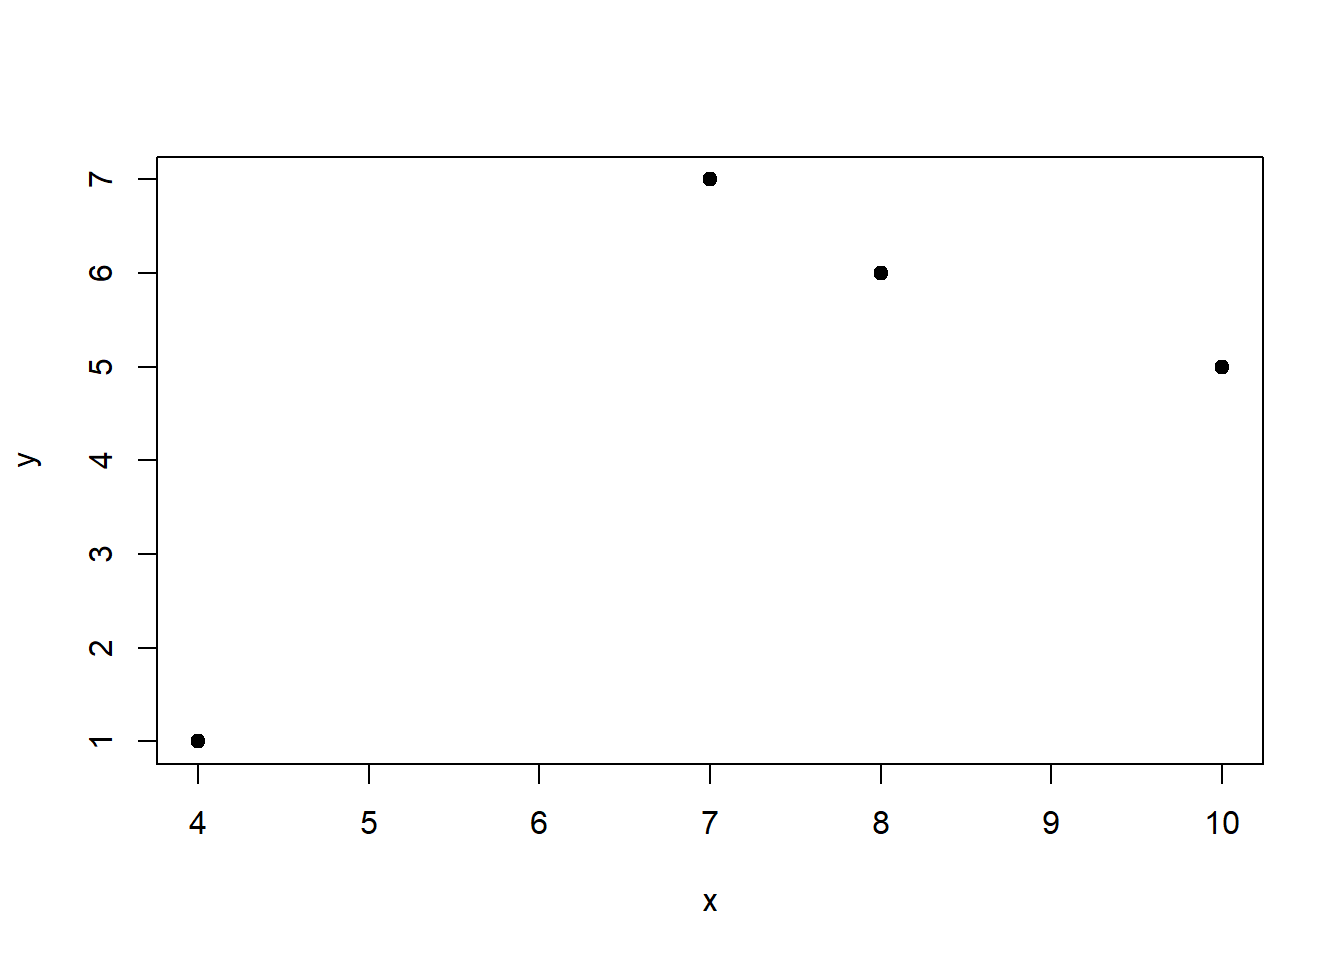
\includegraphics[width=0.75\linewidth]{_main_files/figure-latex/lfit1-1} 

}

\caption{A scatterplot}\label{fig:lfit1}
\end{figure}

The problem is, when you have three or more points, they probably won't lie on the same line, as in the scatterplot in Figure \ref{fig:lfit1}. If they were on a straight line, then we could get \(b_0\) and \(b_1\) by solving the system of equations

\begin{align*}
    b_0+b_1x_1&=y_1\\
    b_0+b_1x_2&=y_2\\
    \vdots &\\
    b_0+b_1x_n&=y_n,
\end{align*}

which we can write in matrix form as

\[\begin{bmatrix}1 & x_1\\1 & x_2\\\vdots & \vdots\\1 & x_n\end{bmatrix}\begin{bmatrix}b_0\\b_1\end{bmatrix}=\begin{bmatrix}y_1\\y_2\\\vdots\\y_n\end{bmatrix}\]

or \(\mathbf{X}\mathbf{b}=\mathbf{y}\). The matrix \(\mathbf{X}\) is called the \emph{design matrix}\index{Design matrix}.

If you do have more than two pairs of points, the system is overdetermined, and there will only be a solution if the points all lie on a straight line. If not, we can, find a least squares approximation. That least squares solution will be \(\hat{\mathbf{b}}\), the solution to the normal equations\index{Normal equations!in linear regression}

\[\mathbf{X}^T\mathbf{X}\mathbf{b}=\mathbf{X}^T\mathbf{y}.\]

It will be unique if the columns of \(X\) are linearly independent. Since there are only two columns in this case, and the first column is all ones, this boils down to having at least two different \(x\) values in the data.

The points on the scatterplot in Figure (\ref{fig:lfit1}) are \((4,1),(8,6),(10,5),\) and \((7,7)\). That makes our system

\[\begin{bmatrix}1 & 4\\1 & 8\\1 & 10\\1 & 7\end{bmatrix}\mathbf{b}=\begin{bmatrix}1\\6\\5\\7\end{bmatrix}.\]

We have

\[\mathbf{X}^T\mathbf{X}=\begin{bmatrix}1 & 1 & 1 & 1\\4 & 8 & 10 & 7\end{bmatrix}\begin{bmatrix}1 & 4\\1 & 8\\1 & 10\\1 & 7\end{bmatrix}=\begin{bmatrix}4 & 29\\29 & 229\end{bmatrix}.\]

Also,

\[\mathbf{X}^T\mathbf{y}=\begin{bmatrix}1 & 1 & 1 & 1\\4 & 8 & 10 & 7\end{bmatrix}\begin{bmatrix}1\\6\\5\\7\end{bmatrix}=\begin{bmatrix}19\\151\end{bmatrix},\]

so our least squares solution is

\[\hat{\mathbf{b}}=\frac{1}{4\cdot229-29\cdot29}\begin{bmatrix}229 & -29\\-29 & 4\end{bmatrix}\begin{bmatrix}19\\151\end{bmatrix}=\frac{1}{75}\begin{bmatrix}-28\\53\end{bmatrix}.\]

Our least squares coefficients are \(\hat{b}_0=-\frac{28}{75}\approx -0.373\) and \(\hat{b}_1=\frac{53}{75}\approx0.707\). When we put the line \(y=-\frac{28}{75}+\frac{53}{75}x\) on the scatterplot, we see the least squares regression line (Fig. \ref{fig:lfit2}). It's not a great fit, mostly because of the point \((4,1).\)

\begin{figure}

{\centering 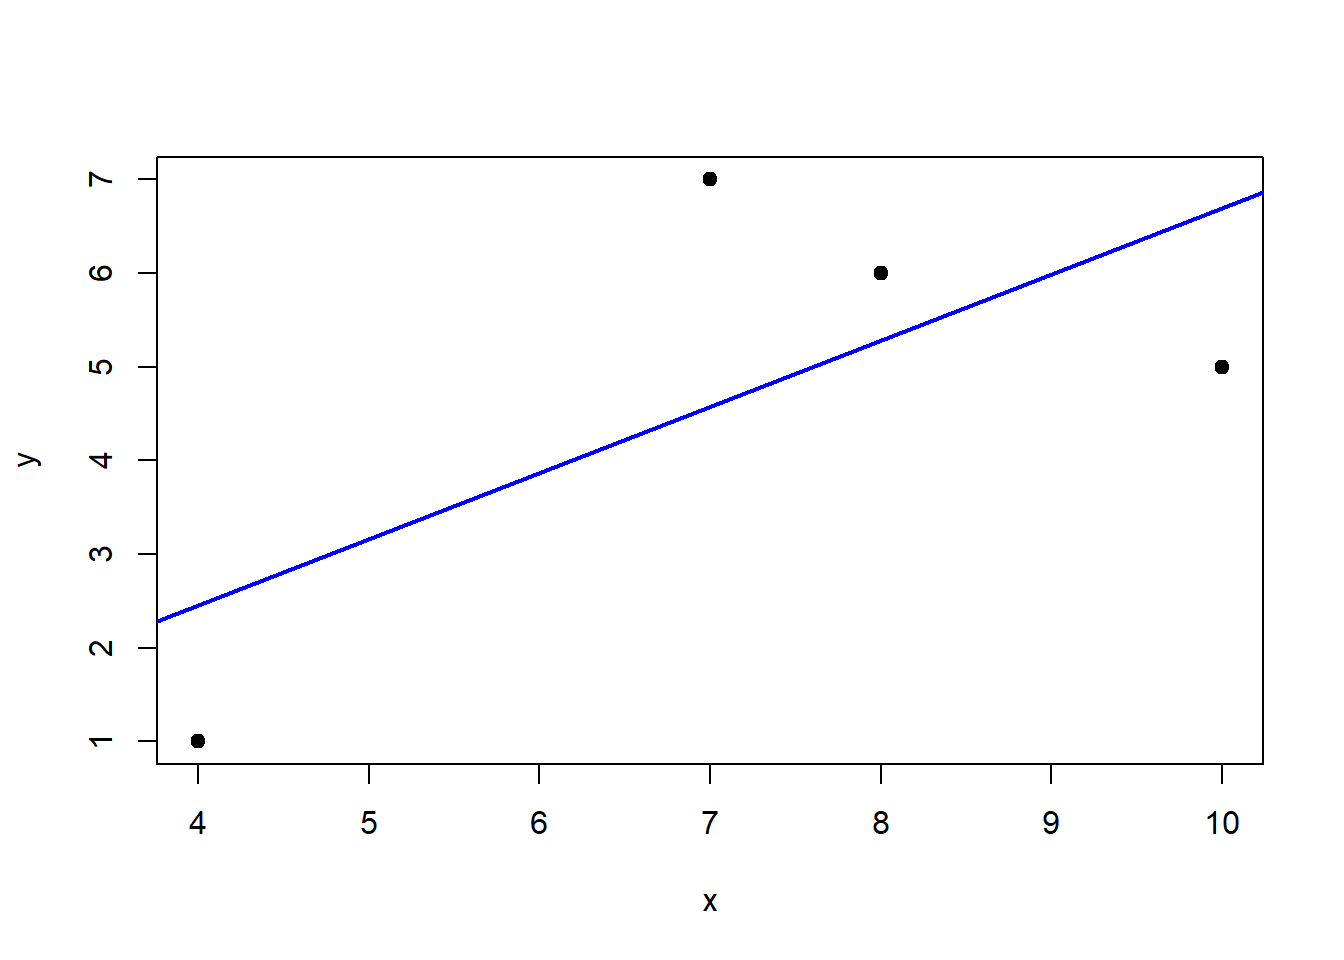
\includegraphics[width=0.75\linewidth]{_main_files/figure-latex/lfit2-1} 

}

\caption{A fitted least squares regression line}\label{fig:lfit2}
\end{figure}

If you've seen regression before, you might wonder how this method compares to that method. Note that

\[\mathbf{X}^T\mathbf{X}=\begin{bmatrix}1 & 1 & \cdots & 1\\x_1 & x_2 & \cdots & x_n\end{bmatrix}\begin{bmatrix}1 & x_1\\1 & x_2\\\vdots & \vdots\\1 & x_n\end{bmatrix}=\begin{bmatrix} n & \sum x_i\\ \sum x_i & \sum x_i^2\end{bmatrix}\]

and

\[\mathbf{X}^T\mathbf{y}=\begin{bmatrix}1 & 1 & \cdots & 1\\x_1 & x_2 & \cdots & x_n\end{bmatrix}\begin{bmatrix}y_1\\y_2\\ \vdots \\y_n\end{bmatrix}=\begin{bmatrix} \sum y_i\\ \sum x_iy_i\end{bmatrix}.\]

All of these terms show up in the formulas for the coefficients that you may have seen. This method produces the same results.

\subsection*{Multilinear regression}\label{multilinear-regression}
\addcontentsline{toc}{subsection}{Multilinear regression}

We can even add independent variables to our least squares linear regression models, without changing the complexity of the mathematical theory.

\begin{examplebox}

\begin{example}
\protect\hypertarget{exm:multilin}{}\label{exm:multilin}Consider the following data in \((x,y,z)\)-form.

\[(1,4,5),(2,3,1),(6,5,2),(2,1,1),(4,3,3)\]

Suppose we want to fit a linear model of the form \(z=b_0+b_1x+b_2y\) to the data. The graph of this function is a plane, and if all of our sample points lie on that plane, then there will be a solution to the following system of equations.

\begin{equation*}
\left\{ \begin{array}{rcl}
b_0+1b_1+4b_2&=5\\
b_0+2b_1+3b_2&=1\\
b_0+6b_1+5b_2&=2\\
b_0+2b_1+1b_2&=1\\
b_0+4b_1+3b_2&=3\\
\end{array}
\right.
\end{equation*}

We can write this in matrix form as

\[\begin{bmatrix} 1 & 1 & 4\\1 & 2 & 3\\1 & 6 & 5\\1 & 2 & 1\\1 & 4 & 3\end{bmatrix}\begin{bmatrix} b_0\\b_1\\b_2\end{bmatrix}=\begin{bmatrix}5\\1\\2\\1\\3\end{bmatrix}\]

or \(\mathbf{X}\mathbf{b}=\mathbf{z}.\) Our matrix \(\mathbf{X}\) has a first column of ones. The second column consists of the \(x\) values, and the third consists of the \(y\) values. The \(\mathbf{z}\) vector contains the \(z\) values. If the points don't lie on a plane we can still find a least squares solution using the normal equations. The least squares solution will be unique if the columns of \(\mathbf{X}\) are linearly independent. Dependence would only occur if \(y\) were a linear function of \(x\) or if \(x\) were a linear function of \(y\). We get

\[\mathbf{X}^T\mathbf{X}=\begin{bmatrix}5 & 15 & 16\\15 & 61 & 54\\16 & 54 & 60\end{bmatrix}\]

and

\[\mathbf{X}^T\mathbf{z}=\begin{bmatrix}12\\33\\43\end{bmatrix}.\]

Our least squares solution is

\[\hat{\mathbf{b}}=(\mathbf{X}^T\mathbf{X})^{-1}\mathbf{X}^T\mathbf{z}=\begin{bmatrix}301/262\\-135/262\\229/262\end{bmatrix}\approx\begin{bmatrix}1.149\\-0.515\\0.874\end{bmatrix}.\]

The equation is

\[z=1.149-0.515x+0.874y.\]
\end{example}

\end{examplebox}

\section{Correlation}\label{CorSec}

It would be nice to have a number to describe how ``linear'' the relationship between two variables is. We have a few of those. The first we will investigate is Pearson's correlation coefficient\index{Correlation!Pearson}.

Here is some motivation for the topic. In Figure \ref{fig:posslope}, we have data where \(y\) is a linear function of \(x\) with positive slope. On the right, we have ``centered'' the data by subtracting the \(x\) mean from the \(x\) values and the \(y\) mean from the \(y\) values. Let's call the centered values \(\hat{x}\) and \(\hat{y}\). When we do this, we get points that are on a line with the same slope, and the intercept is 0.

\begin{figure}
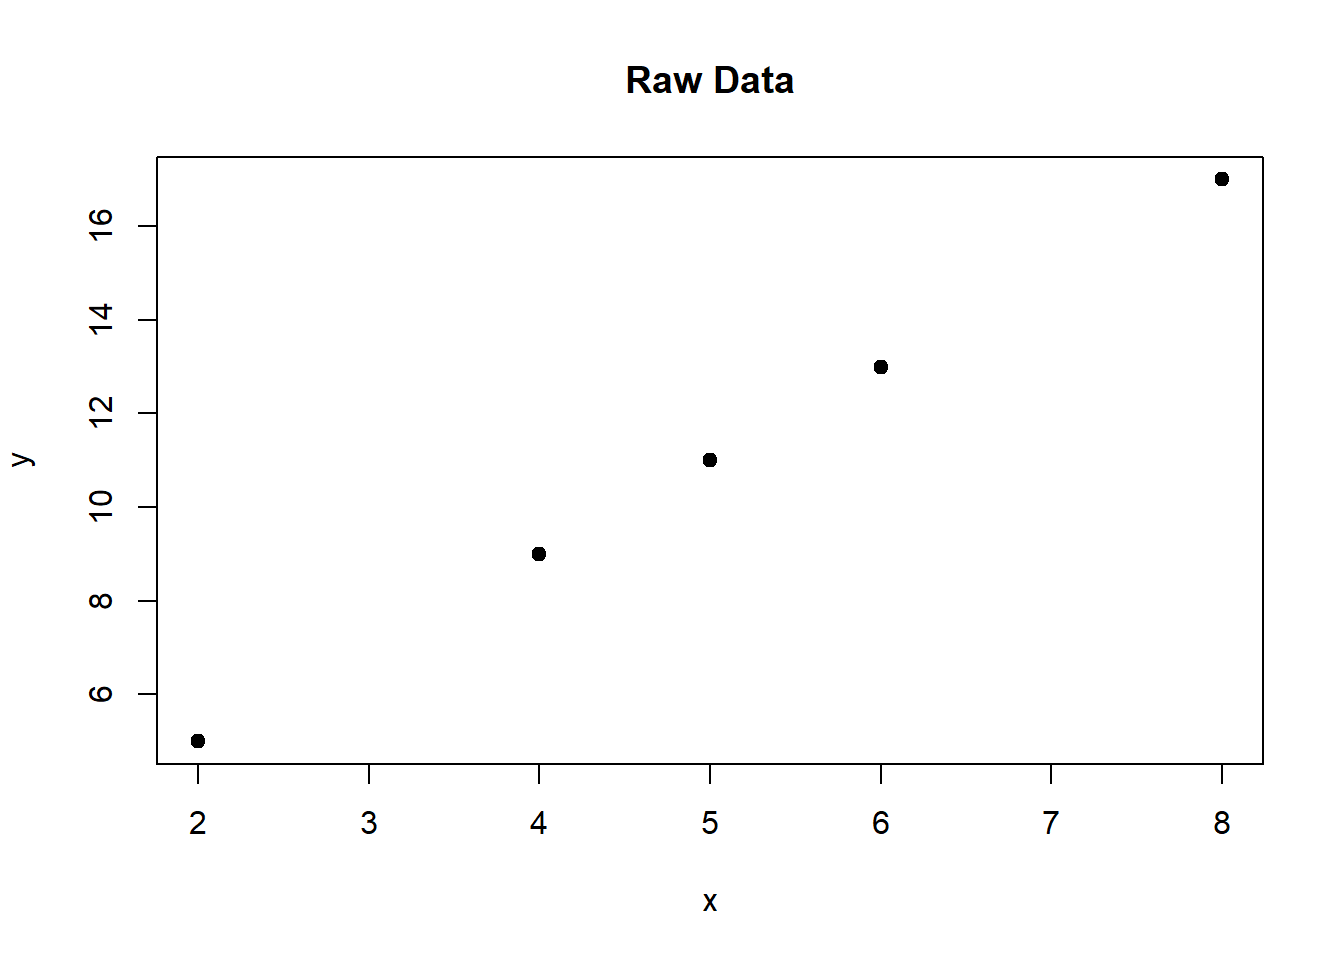
\includegraphics[width=0.5\linewidth]{_main_files/figure-latex/posslope-1} 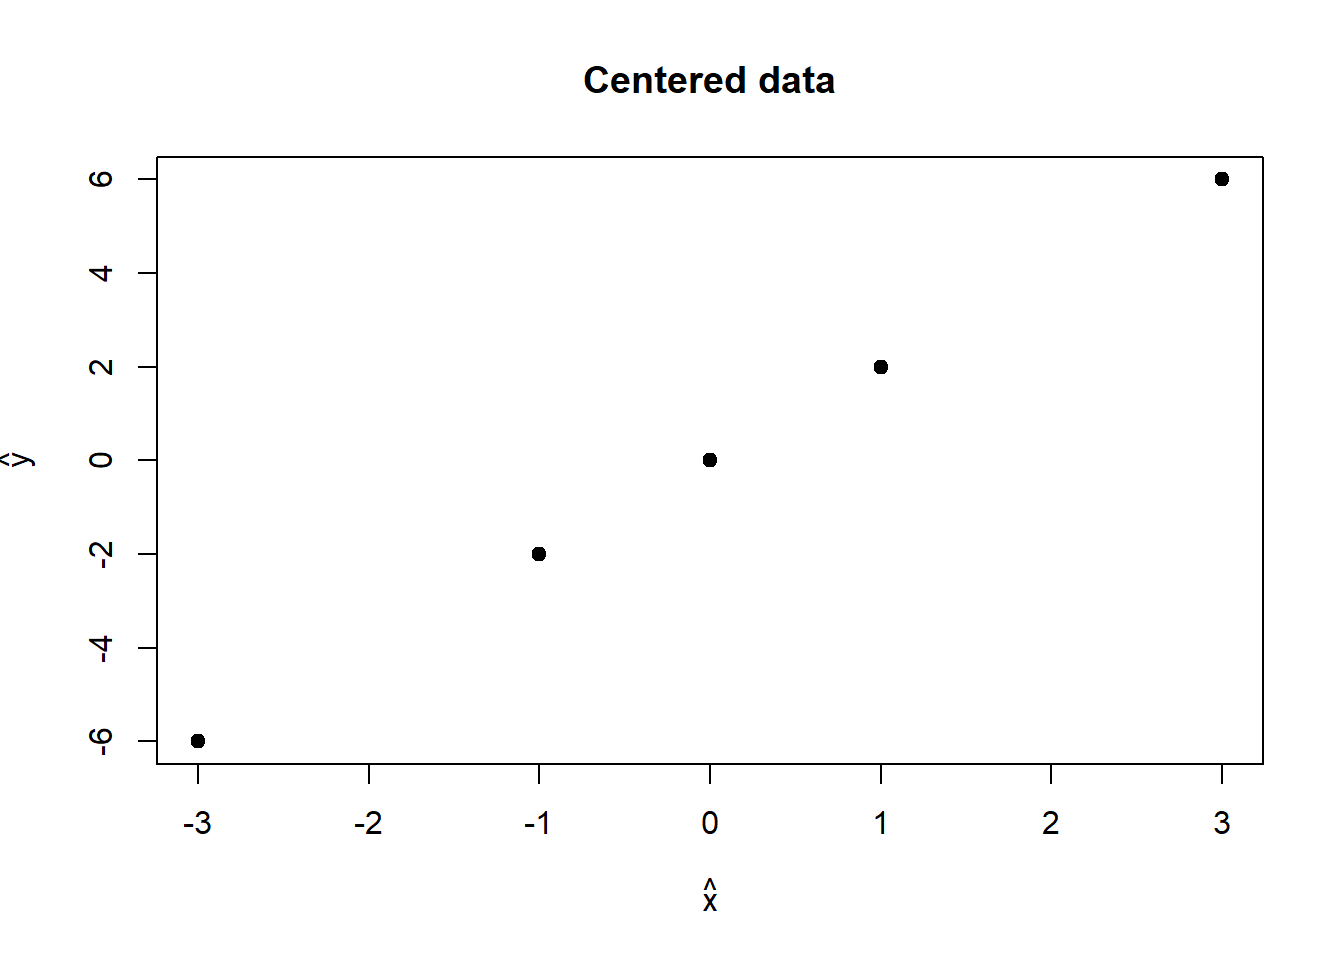
\includegraphics[width=0.5\linewidth]{_main_files/figure-latex/posslope-2} \caption{Centering data}\label{fig:posslope}
\end{figure}

If we put the centered values in vectors, \(\hat{\mathbf{x}}\) and \(\hat{\mathbf{y}}\), we have \(\hat{\mathbf{y}}=m\hat{\mathbf{x}},\) where \(m\) is the positive slope. We can't see the \(\hat{\mathbf{x}}\) and \(\hat{\mathbf{y}}\) vectors because they live in \(\mathbb{R}^5\), but the vectors are pointing in the same direction, so the angle between them, \(\theta,\) is \(0^{\circ}.\)

\begin{figure}
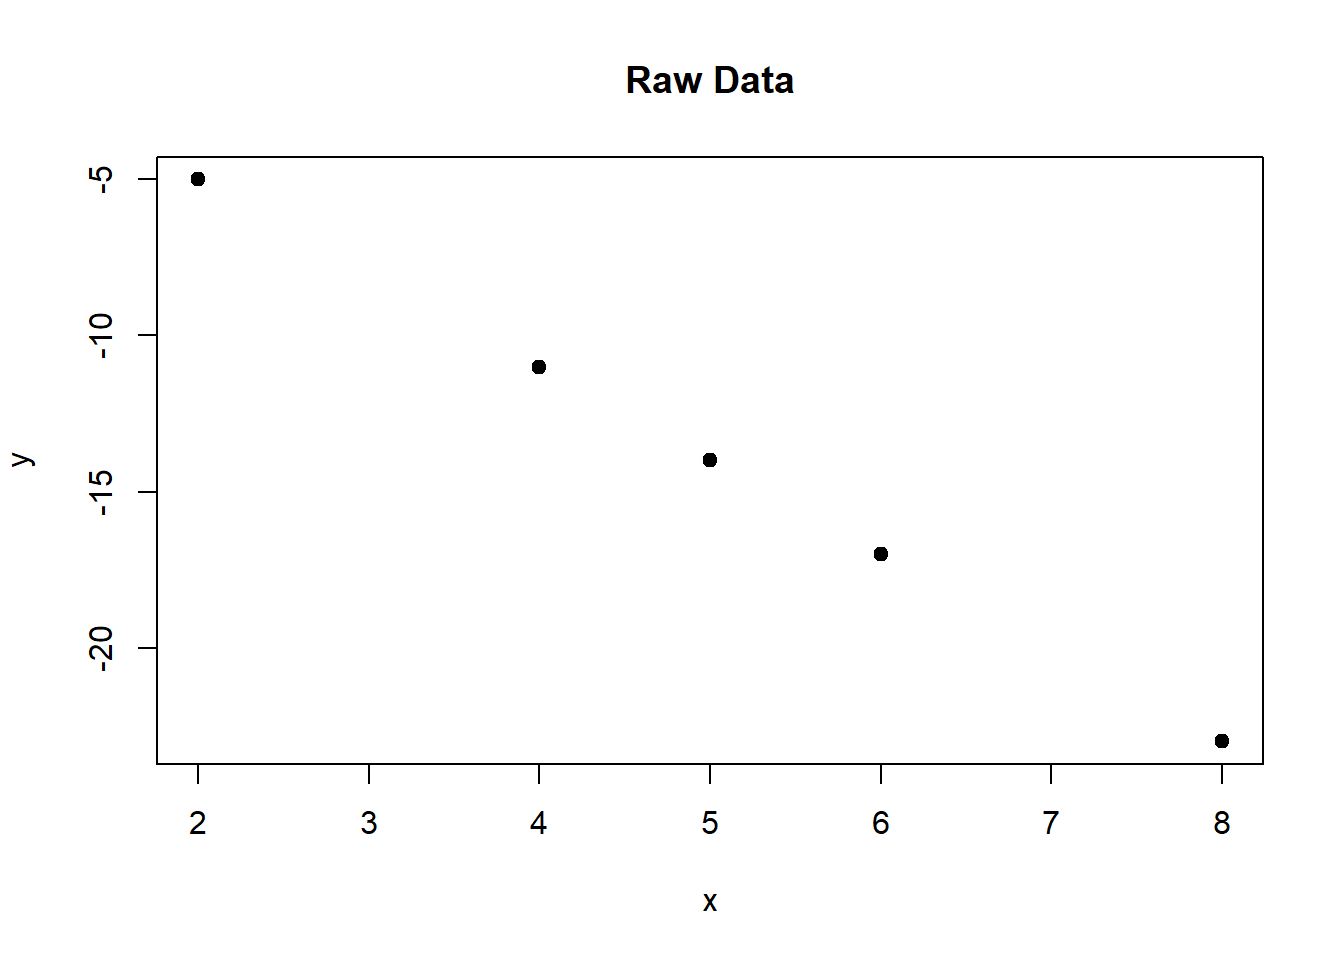
\includegraphics[width=0.5\linewidth]{_main_files/figure-latex/negslope-1} 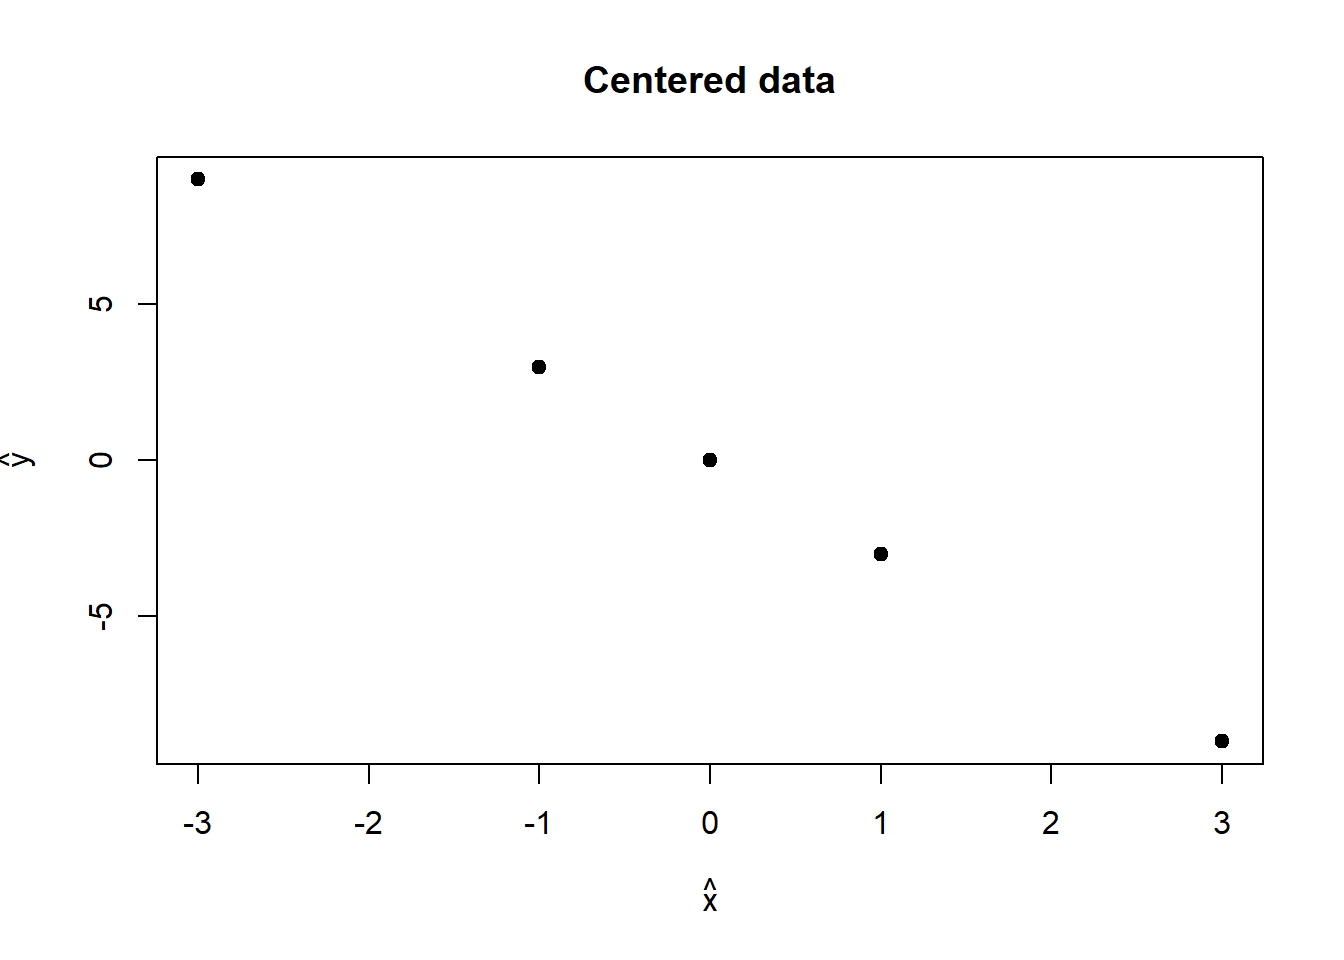
\includegraphics[width=0.5\linewidth]{_main_files/figure-latex/negslope-2} \caption{Negative slope}\label{fig:negslope}
\end{figure}

In Figure \ref{fig:negslope}, the points lie on a straight line with negative slope. When we center the values, the angle between the centered vectors is \(180^{\circ}.\)

Recall that the angle between two vectors satisfies Equation \eqref{eq:lawofcosines}

\[\cos\theta=\frac{\mathbf{u}\cdot \mathbf{v}}{|\mathbf{u}||\mathbf{v}|}.\]

For the points on the line with positive slope, we have \(\cos\theta=1,\) and for the points on the line with negative slope, we have \(\cos\theta=-1.\) If points are not on a straight line, the angle between the centered vector will be between \(0^{\circ}\) and \(180^{\circ},\) and the cosine of that angle will be between \(-1\) and \(1.\) We're going to call this number \(r.\)

\subsection*{Some notation and a formula}\label{some-notation-and-a-formula}
\addcontentsline{toc}{subsection}{Some notation and a formula}

If our points are \((x_1,y_1),\dots,(x_n,y_n),\) then the dot product of the centered vectors is

\[\hat{\mathbf{x}}\cdot\hat{\mathbf{y}}=(x_1-\bar{x})(y_1-\bar{y})+\cdots+(x_n-\bar{x})(y_n-\bar{y})=\sum_{i=1}^n (x_i-\bar{x})(y_i-\bar{y}).\]

The ``sigma notation''\index{Sigma notation} means we are adding all terms of the form \((x_i-\bar{x})(y_i-\bar{y})\) with subscripts \(i\) running from 1 to \(n.\)

The magnitudes of \(\hat{\mathbf{x}}\) and \(\hat{\mathbf{y}}\) can be written as

\[\sqrt{(x_1-\bar{x})^2+\cdots+(x_n-\bar{x})^2}=\sqrt{\sum_{i=1}^n(x_i-\bar{x})^2}\]

and

\[\sqrt{\sum_{i=1}^n(y_i-\bar{y})^2}.\]

This gives our formula for Pearson's correlation coefficient.

\begin{equation}
r=\frac{\sum_{i=1}^n (x_i-\bar{x})(y_i-\bar{y})}{\sqrt{\sum_{i=1}^n(x_i-\bar{x})^2}\sqrt{\sum_{i=1}^n(y_i-\bar{y})^2}}
\label{eq:pearson}
\end{equation}

We can get these terms using matrices as follows. Let

\[
\mathbf{B}=\begin{bmatrix}\hat{\mathbf{x}} & \hat{\mathbf{y}}\end{bmatrix}=\begin{bmatrix} x_1-\bar{x} & y_1-\bar{y}\\ \vdots & \vdots \\ x_n-\bar{x} & y_n-\bar{y}\end{bmatrix}.\]

Then

\begin{align*}
\mathbf{B}^T \mathbf{B}&=\begin{bmatrix} x_1-\bar{x} & \cdots & x_n-\bar{x}\\  x_1-\bar{y} & \cdots & y_n-\bar{y}\end{bmatrix} \begin{bmatrix} x_1-\bar{x} & y_1-\bar{y}\\ \vdots & \vdots \\ x_n-\bar{x} & y_n-\bar{y}\end{bmatrix}\\
&=\begin{bmatrix} \sum_{i=1}^n(x_i-\bar{x})^2 & \sum_{i=1}^n (x_i-\bar{x})(y_i-\bar{y})\\ \sum_{i=1}^n (x_i-\bar{x})(y_i-\bar{y}) & \sum_{i=1}^n(y_i-\bar{y})^2\end{bmatrix}.
\end{align*}

Note: the matrix \(\mathbf{S}=\frac{1}{n-1}\mathbf{B}^T \mathbf{B}\) is called the \emph{covariance matrix}\index{Covariance matrix} (or \emph{sample covariance matrix}). The diagonal entries of \(\mathbf{S}\) give the sample variance\index{Variance} for the corresponding values, while the off-diagonal entries give the sample covariance\index{Covariance}, which is like an unscaled version of the correlation coefficient. We will see this matrix again when we study principal component analysis.

Before we do some calculations, here are some properties of \(r.\)

\begin{propbox}

\textbf{Properties of Pearson's Correlation Coefficient} \(r\)

\begin{enumerate}
\def\labelenumi{\arabic{enumi}.}
\item
  \(-1\leq r\leq 1\)
\item
  If \(r=1,\) there is perfect positive correlation: all of the \((x,y)\) pairs lie on a straight line with positive slope.
\item
  If \(r=-1,\) there is perfect negative correlation.
\item
  The closer \(r\) is to \(1\) or \(-1,\) the stronger the correlation.
\item
  The closer \(r\) is to \(0,\) the weaker the \emph{linear} correlation. There may be some other type of correlation. It is always a good idea to look at a scatterplot to see if there is some sort of non-linear trend in the data.
\end{enumerate}

\end{propbox}

Correlation computations are almost always performed using calculators or software packages, but sometimes it is illustrative to do calculations by hand. In that case, there are some formulas that make it a little easier to do hand calculations. Here they are

\begin{equation}
S_{xx}=\sum_{i=1}^n(x_i-\bar{x})^2=\left(\sum_{i=1}^n x_i^2\right)-n\bar{x}^2
\label{eq:Sxx}
\end{equation}

\begin{equation}
S_{yy}=\sum_{i=1}^n(y_i-\bar{y})^2=\left(\sum_{i=1}^n y_i^2\right)-n\bar{y}^2
\label{eq:Syy}
\end{equation}

\begin{equation}
S_{xy}=\sum_{i=1}^n (x_i-\bar{x})(y_i-\bar{y})=\left(\sum_{i=1}^n x_iy_i\right)-n\bar{x}\bar{y} 
\label{eq:Sxy}
\end{equation}

These allow us to write the correlation coefficient as

\begin{equation}
r=\frac{S_{xy}}{\sqrt{S_{xx}S_{yy}}}.
\label{eq:PCC}
\end{equation}

The terms \(\sum_{i=1}^nx_i^2\) and \(\sum_{i=1}^ny_i^2\) mean we square the \(x\) and \(y\) values and add them up. The \(\sum_{i=1}^n x_iy_i\) means we multiply each \((x_i,y_i)\) pair and add them up. These terms show up frequently in statistical settings.

\begin{examplebox}

\begin{example}
Here is a simple example with five nice pairs of points. The sums appear in bold at the bottom.

\begin{longtable}[]{@{}lllll@{}}
\toprule\noalign{}
\(x_i\) & \(y_i\) & \(x_i^2\) & \(y_i^2\) & \(x_i y_i\) \\
\midrule\noalign{}
\endhead
\bottomrule\noalign{}
\endlastfoot
4 & 2 & 16 & 4 & 8 \\
-1 & 3 & 1 & 9 & -3 \\
5 & 2 & 25 & 4 & 10 \\
2 & -3 & 4 & 9 & -6 \\
0 & 1 & 0 & 1 & 0 \\
\textbf{10} & \textbf{5} & \textbf{46} & \textbf{27} & \textbf{9 } \\
\end{longtable}

We have \(\bar{x}=10/5=2,\bar{y}=5/5=1,S_{xx}=46-5*2^2=26, S_{yy}=27-5*1^2=22,\) and \(S_{xy}=9-5*2*1=-1,\) so \(r=\dfrac{-1}{\sqrt{26*22}}=-0.042.\) This is very weak negative linear correlation, as you can see from the scatterplot (Fig. \ref{fig:weak}).
\end{example}

\end{examplebox}

\begin{figure}

{\centering 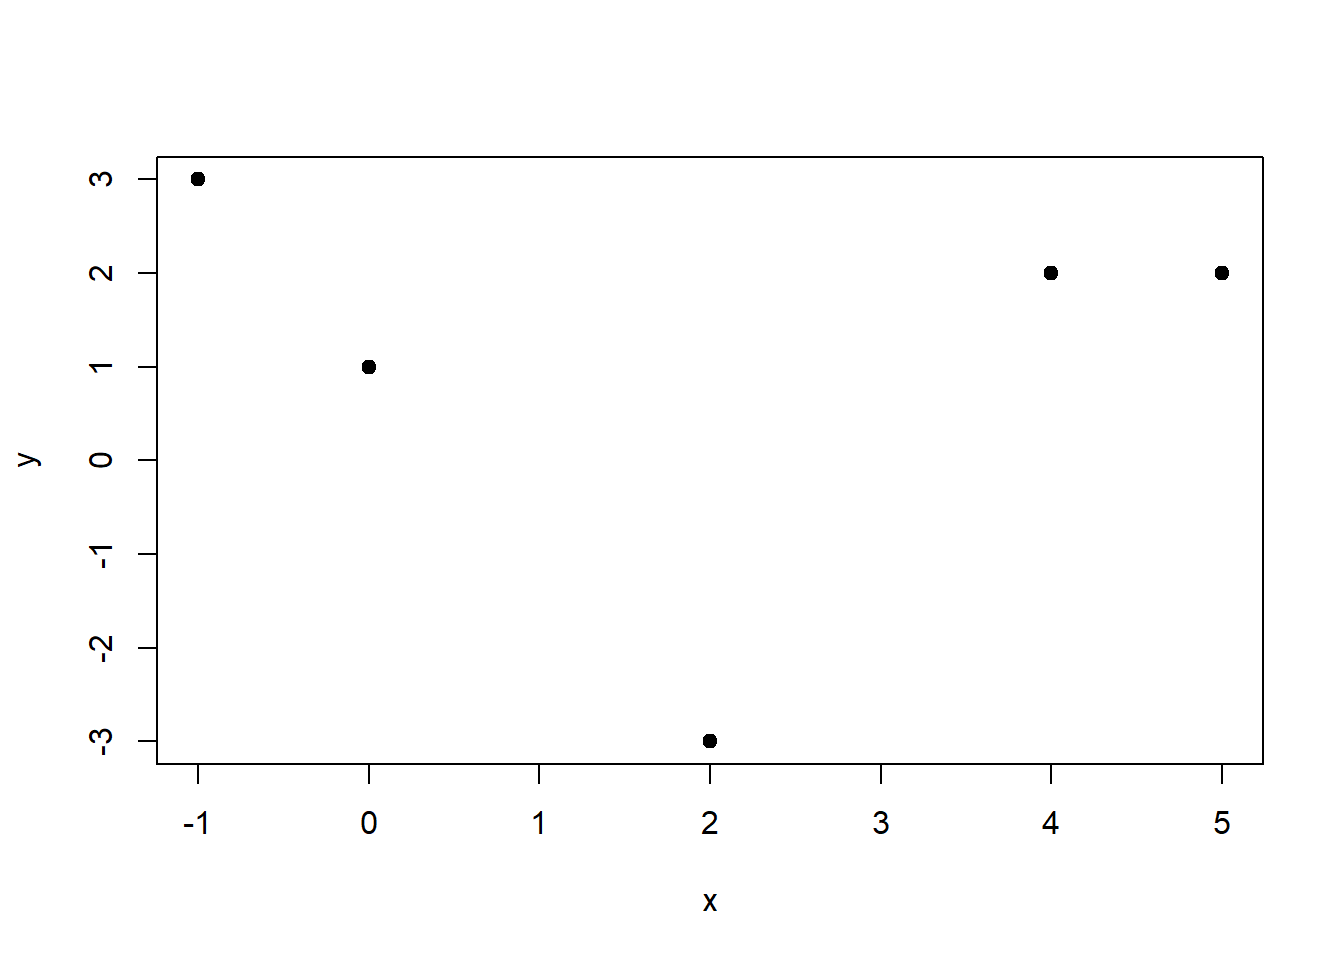
\includegraphics[width=0.75\linewidth]{_main_files/figure-latex/weak-1} 

}

\caption{Weak correlation}\label{fig:weak}
\end{figure}

\begin{examplebox}

\begin{example}
\protect\hypertarget{exm:requalneg1}{}\label{exm:requalneg1}\leavevmode

\begin{longtable}[]{@{}lllll@{}}
\toprule\noalign{}
\(x_i\) & \(y_i\) & \(x_i^2\) & \(y_i^2\) & \(x_i y_i\) \\
\midrule\noalign{}
\endhead
\bottomrule\noalign{}
\endlastfoot
1 & 9 & 1 & 81 & 9 \\
4 & 3 & 16 & 9 & 12 \\
2 & 7 & 4 & 49 & 14 \\
5 & 1 & 25 & 1 & 5 \\
\textbf{12} & \textbf{20} & \textbf{46} & \textbf{140} & \textbf{40} \\
\end{longtable}

With \(n=4\) this time, \(\bar{x}=12/4=3\) and \(\bar{y}=20/4=5.\) That gives us \(S_{xx}=46-4\cdot3^2=10,S_{yy}=140-4\cdot 5^2=40,\) and \(S_{xy}=40-4\cdot 3\cdot 5=-20.\) So,

\[r=\frac{-20}{\sqrt{10\cdot40}}=-1.\]

Our points lie on a straight line with negative slope (Fig. \ref{fig:ns}).

\end{example}

\end{examplebox}

\begin{figure}

{\centering 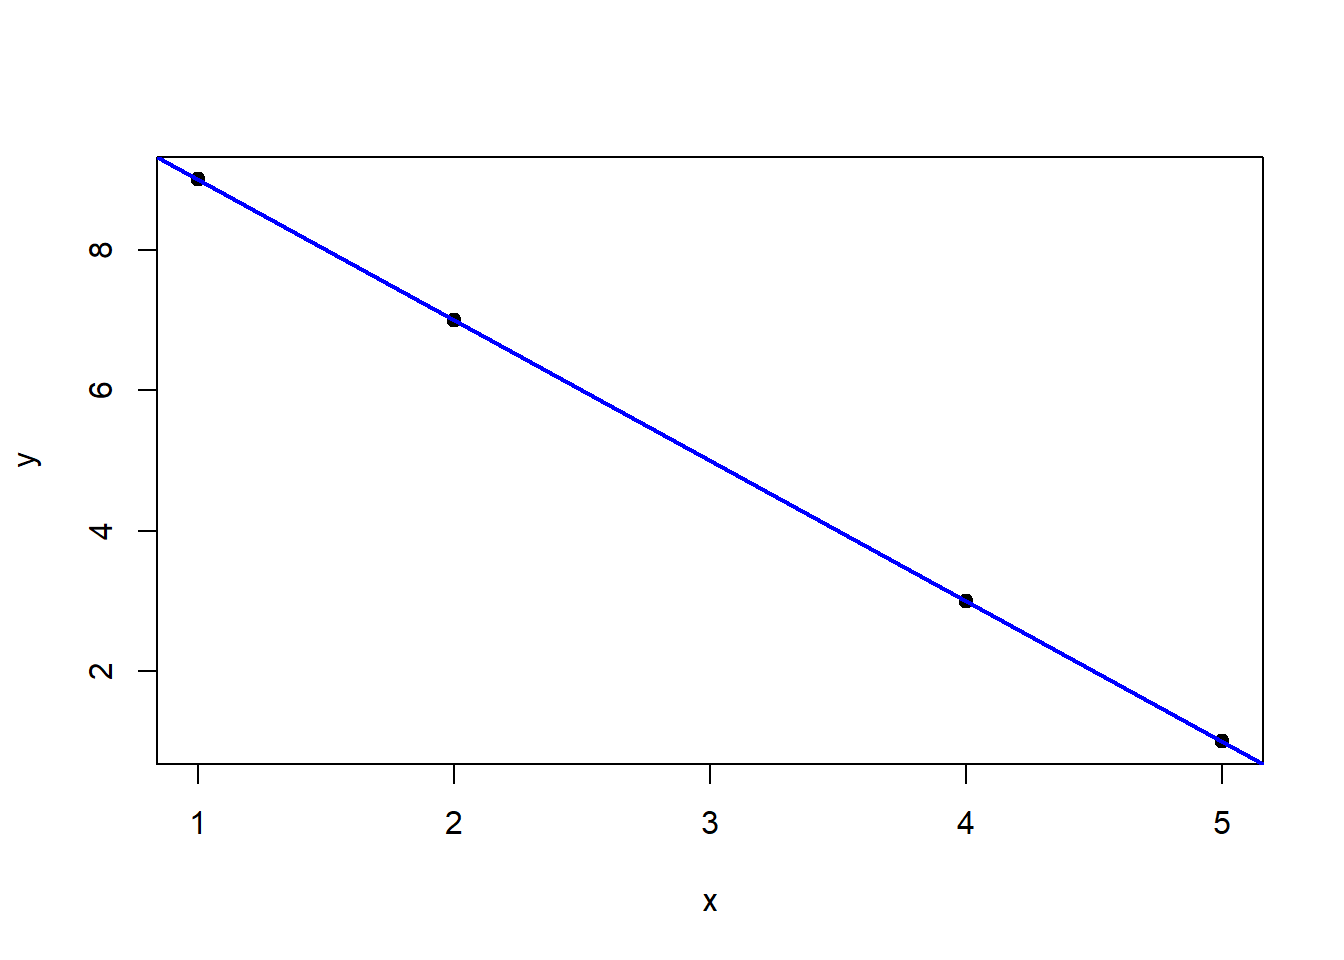
\includegraphics[width=0.75\linewidth]{_main_files/figure-latex/ns-1} 

}

\caption{Perfect negative correlation}\label{fig:ns}
\end{figure}

\begin{examplebox}

\begin{example}
Here is one last simple example.

\begin{longtable}[]{@{}lllll@{}}
\toprule\noalign{}
\(x_i\) & \(y_i\) & \(x_i^2\) & \(y_i^2\) & \(x_i y_i\) \\
\midrule\noalign{}
\endhead
\bottomrule\noalign{}
\endlastfoot
-2 & 4 & 4 & 16 & -8 \\
-1 & 1 & 1 & 1 & -1 \\
0 & 0 & 0 & 0 & 0 \\
1 & 1 & 1 & 1 & 1 \\
2 & 4 & 4 & 16 & 8 \\
\textbf{0} & \textbf{10} & \textbf{10} & \textbf{34} & \textbf{0 } \\
\end{longtable}

We have \(\bar{x}=0,\bar{y}=10/5=2,\) and \(S_{xy}=0-5\cdot0\cdot2\), so \(r=0.\) There is no linear correlation between the \(x\) and \(y\) values. We should always look at the scatterplot, though. Figure \ref{fig:nonlinear} tells us what we should have noticed from the table of values. The points all lie on the parabola \(y=x^2.\)
\end{example}

\end{examplebox}

\begin{figure}

{\centering 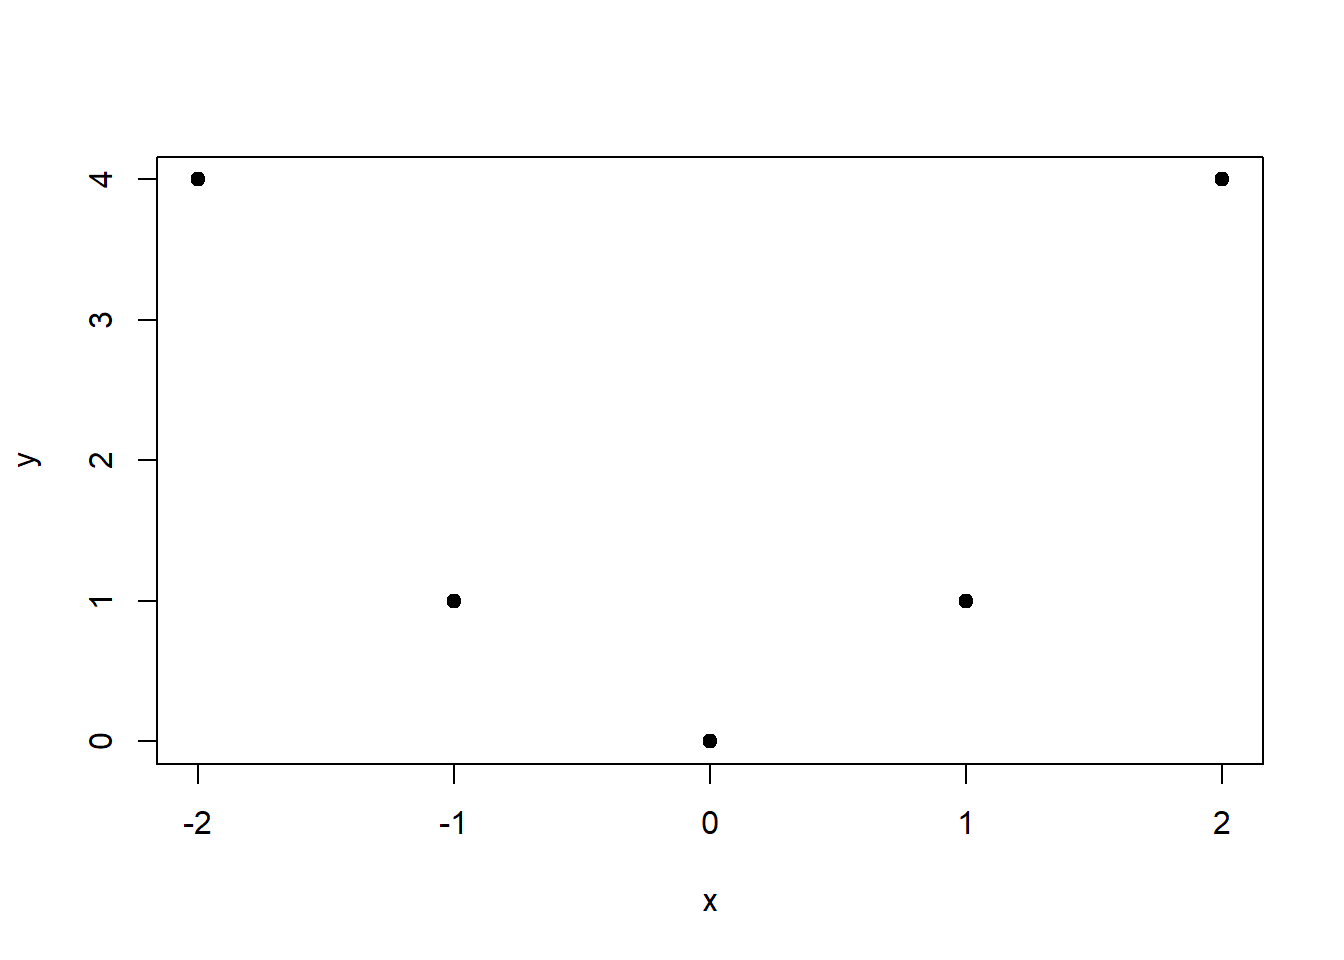
\includegraphics[width=0.75\linewidth]{_main_files/figure-latex/nonlinear-1} 

}

\caption{Always look at the scatterplot}\label{fig:nonlinear}
\end{figure}

\pagebreak

\subsection*{Correlation in R}\label{correlation-in-r}
\addcontentsline{toc}{subsection}{Correlation in R}

The \texttt{cor} function in R will calculate Pearson's and other correlation coefficients. Pearson's is the default.

\begin{Shaded}
\begin{Highlighting}[]
\FunctionTok{cor}\NormalTok{(mtcars}\SpecialCharTok{$}\NormalTok{wt,mtcars}\SpecialCharTok{$}\NormalTok{mpg)}
\end{Highlighting}
\end{Shaded}

\begin{verbatim}
## [1] -0.8676594
\end{verbatim}

The \texttt{with} function makes it easier to work with data frames.

\begin{Shaded}
\begin{Highlighting}[]
\FunctionTok{with}\NormalTok{(mtcars, }\FunctionTok{cor}\NormalTok{(wt,mpg))}
\end{Highlighting}
\end{Shaded}

\begin{verbatim}
## [1] -0.8676594
\end{verbatim}

Figure \ref{fig:with} shows the scatterplot.

\begin{figure}

{\centering 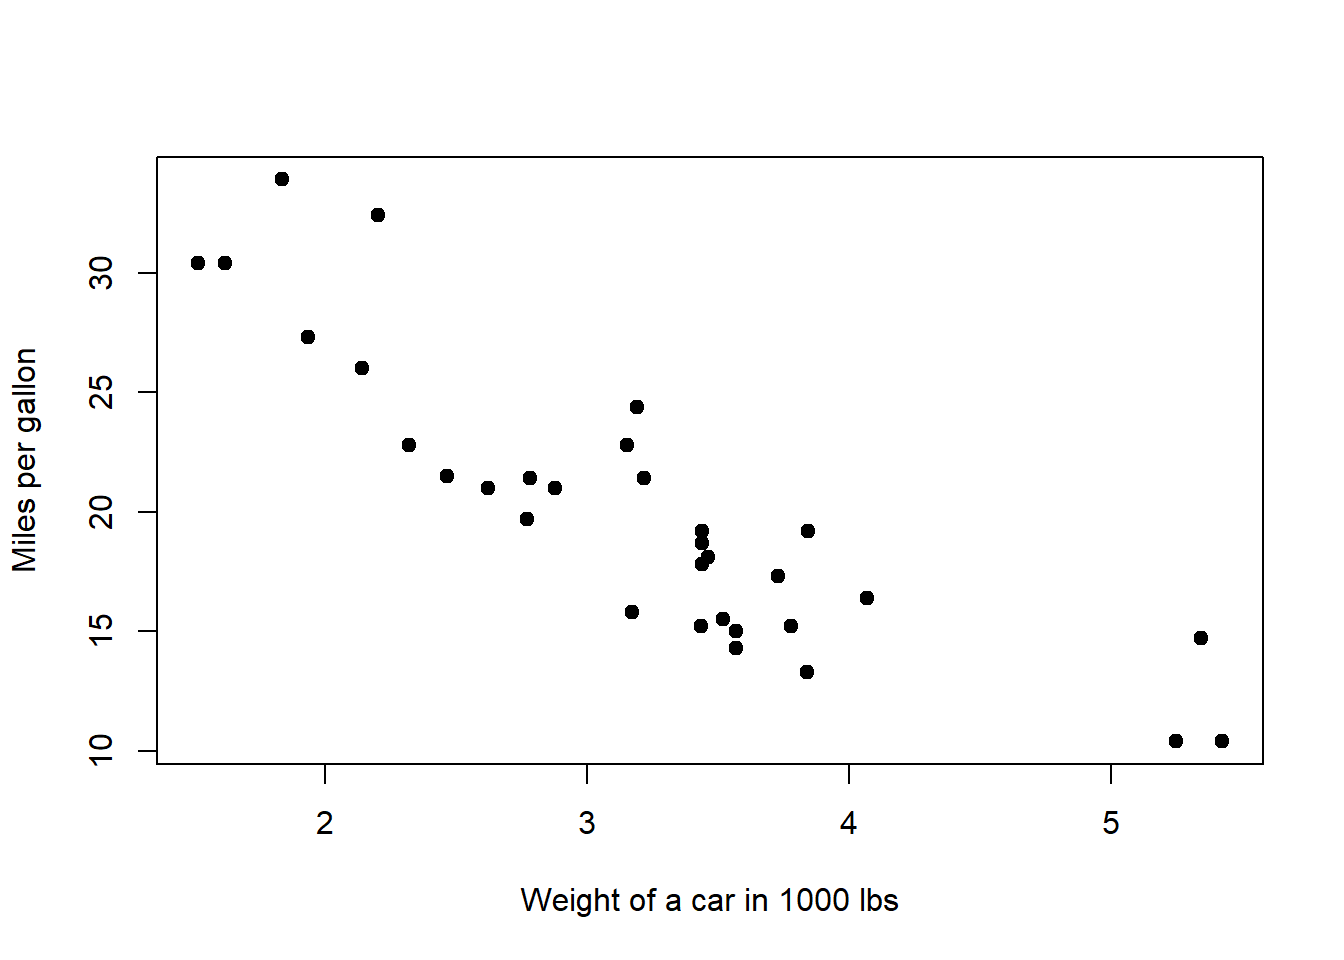
\includegraphics[width=0.75\linewidth]{_main_files/figure-latex/with-1} 

}

\caption{Miles per gallon and weight have a strong negative correlation}\label{fig:with}
\end{figure}

If you use the \texttt{cor} function on a numerical data frame, you get a table of pairwise correlations. Note that the correlation of a variable with itself is always 1.

\begin{Shaded}
\begin{Highlighting}[]
\FunctionTok{round}\NormalTok{(}\FunctionTok{cor}\NormalTok{(mtcars), }\DecValTok{2}\NormalTok{)}
\end{Highlighting}
\end{Shaded}

\begin{verbatim}
##        mpg   cyl  disp    hp  drat    wt  qsec    vs    am  gear  carb
## mpg   1.00 -0.85 -0.85 -0.78  0.68 -0.87  0.42  0.66  0.60  0.48 -0.55
## cyl  -0.85  1.00  0.90  0.83 -0.70  0.78 -0.59 -0.81 -0.52 -0.49  0.53
## disp -0.85  0.90  1.00  0.79 -0.71  0.89 -0.43 -0.71 -0.59 -0.56  0.39
## hp   -0.78  0.83  0.79  1.00 -0.45  0.66 -0.71 -0.72 -0.24 -0.13  0.75
## drat  0.68 -0.70 -0.71 -0.45  1.00 -0.71  0.09  0.44  0.71  0.70 -0.09
## wt   -0.87  0.78  0.89  0.66 -0.71  1.00 -0.17 -0.55 -0.69 -0.58  0.43
## qsec  0.42 -0.59 -0.43 -0.71  0.09 -0.17  1.00  0.74 -0.23 -0.21 -0.66
## vs    0.66 -0.81 -0.71 -0.72  0.44 -0.55  0.74  1.00  0.17  0.21 -0.57
## am    0.60 -0.52 -0.59 -0.24  0.71 -0.69 -0.23  0.17  1.00  0.79  0.06
## gear  0.48 -0.49 -0.56 -0.13  0.70 -0.58 -0.21  0.21  0.79  1.00  0.27
## carb -0.55  0.53  0.39  0.75 -0.09  0.43 -0.66 -0.57  0.06  0.27  1.00
\end{verbatim}

To isolate a single variable's correlations, you can use code like the following.

\begin{Shaded}
\begin{Highlighting}[]
\FunctionTok{cor}\NormalTok{(mtcars}\SpecialCharTok{$}\NormalTok{mpg,mtcars)}
\end{Highlighting}
\end{Shaded}

\section{Formulas for Least Squares Regression}\label{formulas-for-least-squares-regression}

In this section, we are going to approach least squares regression from a slightly different perspective from that in Section \ref{LSRSec}.

If we determine that two variables are linearly correlated, we would like to find an equation \(\hat{y}=\hat{b}_0+\hat{b}_1x\) that best fits the data. (The value \(\hat{y}\) is the predicted or average value of \(y\) for a given \(x\) value.)

\begin{figure}

{\centering 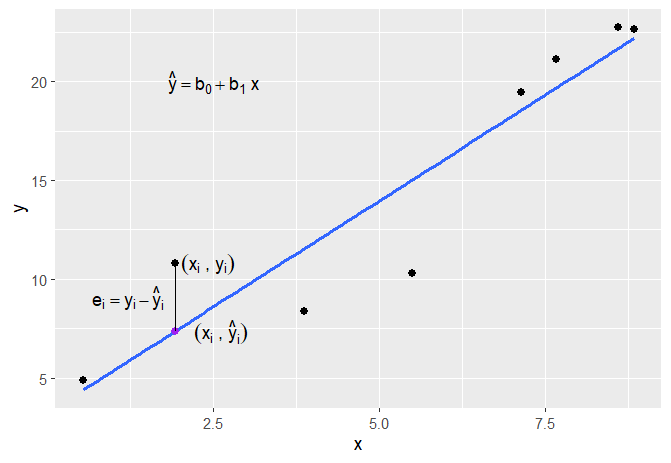
\includegraphics[width=0.7\linewidth]{images/residuals} 

}

\caption{Minimizing the residuals}\label{fig:residuals}
\end{figure}

The goal is to somehow minimize the \emph{residuals}\index{Residuals} \(e_i=y_i-\hat{y}_i.\) (See Fig. \ref{fig:residuals}.) In any ``best'' fit, some points will be above the line, and some will be below the line. Because of this, some residuals will be positive, and some will be negative. The least-squares solution minimizes the sum of the \emph{squares} of the residuals so there's no cancellation.

\begin{propbox}
\textbf{The Least Squares Problem}

Find coefficients \(\hat{b}_0\) and \(\hat{b}_1\) that minimize

\[S=\sum_{i=1}^n (y_i-\hat{y}_i)^2,\]

where \(\hat{y}_i=\hat{b}_0+\hat{b}_1 x_i.\)

\end{propbox}

Note: this is a multivariable calculus problem. For a short introduction to, or review of, the material, consult Appendix A. The sum we are trying to minimize

\[S=\sum_{i=1}^n (y_i-\hat{y}_i)^2=\sum_{i=1}^n(y_i-\hat{b}_0-\hat{b}_1x_i)^2\]

is a function of two variables, \(\hat{b}_0\) and \(\hat{b}_1\). We can minimize it by finding the critical point, i.e., the solution to

\[\frac{\partial S}{\partial \hat{b}_0}=0\text{ and }\frac{\partial S}{\partial \hat{b}_1}=0.\]

Remember that the derivative of a sum is the sum of the derivatives, and that holds for partial differentiation, too. The value \(S\) is just a sum of a bunch of squared terms. With

\[S=\sum_{i=1}^n(y_i-\hat{b}_0-\hat{b}_1x_i)^2,\]

\begin{equation}
\frac{\partial S}{\partial \hat{b}_0}=\sum_{i=1}^n 2(y_i-\hat{b}_0-\hat{b}_1x_i)(-1)=0,
\label{eq:b0partial}
\end{equation}

and

\begin{equation}
\frac{\partial S}{\partial \hat{b}_1}=\sum_{i=1}^n 2(y_i-\hat{b}_0-\hat{b}_1x_i)(-x_i)=0.
\label{eq:b1partial}
\end{equation}

We can divide by \(-2\) and rearrange things. From \eqref{eq:b0partial}, We have

\[\sum_{i=1}^n (y_i-\hat{b}_0-\hat{b}_1x_i)=0\Rightarrow \sum_{i=1}^ny_i=\sum_{i=1}^n \hat{b}_0+\sum_{i=1}^n\hat{b}_1x_i\]

We can rewrite this as

\[n\bar{y}=n\hat{b}_0+\hat{b}_1n\bar{x}\]

or

\begin{equation}
\boxed{\hat{b}_0=\bar{y}-\hat{b}_1\bar{x}.}
\label{eq:intercept}
\end{equation}

Now we need to find \(\hat{b}_1\).

Setting \(\partial S/\partial \hat{b}_1\) \eqref{eq:b1partial} equal to zero and dividing by \(-2\) gives us

\[\sum_{i=1}^n (y_i-\hat{b}_0-\hat{b}_1x_i)(x_i)=0\Rightarrow \sum_{i=1}^n x_iy_i=\sum_{i=1}^n \hat{b}_0x_i+\sum_{i=1}^n\hat{b}_1x_i^2,\]

or

\[\hat{b}_1\sum_{i=1}^n x_i^2=\left(\sum_{i=1}^nx_iy_i\right)-\hat{b}_0 n\bar{x}=\left(\sum_{i=1}^nx_iy_i\right)-(\bar{y}-\hat{b}_1\bar{x})n\bar{x}.\]

Collecting the \(\hat{b}_1\) terms gives us

\[\hat{b}_1\left(\left(\sum_{i=1}^nx_i^2\right)-n\bar{x}^2\right)=\left(\sum_{i=1}^nx_iy_i\right)-n\bar{x}\bar{y}\]

or

\begin{equation}
\boxed{\hat{b}_1=\frac{\left(\sum_{i=1}^nx_iy_i\right)-n\bar{x}\bar{y}}{\left(\sum_{i=1}^nx_i^2\right)-n\bar{x}^2}=\frac{S_{xy}}{S_{xx}},}
\label{eq:slope}
\end{equation}

where \(S_{xy}\) and \(S_{xx}\) are defined in Equations \eqref{eq:Sxy} and \eqref{eq:Sxx}, respectively. Let's summarize our results.

\begin{propbox}
\textbf{The Least Squares Equation}

The linear least-squares equation is \(\hat{y}=\hat{b}_0+\hat{b}_1 x,\) where \(\hat{b}_1=\dfrac{S_{xy}}{S_{xx}},\) and \(\hat{b}_0=\bar{y}-\hat{b}_1 \bar{x}.\)

\end{propbox}

\begin{examplebox}

\begin{example}
First, let's check to make sure that our formula works for truly linear data. Here is the data from Example \ref{exm:requalneg1}.

\begin{longtable}[]{@{}lllll@{}}
\toprule\noalign{}
\(x_i\) & \(y_i\) & \(x_i^2\) & \(y_i^2\) & \(x_i y_i\) \\
\midrule\noalign{}
\endhead
\bottomrule\noalign{}
\endlastfoot
1 & 9 & 1 & 81 & 9 \\
4 & 3 & 16 & 9 & 12 \\
2 & 7 & 4 & 49 & 14 \\
5 & 1 & 25 & 1 & 5 \\
\textbf{12} & \textbf{20} & \textbf{46} & \textbf{140} & \textbf{40} \\
\end{longtable}

Again, \(\bar{x}=3, \bar{y}=5, S_{xy}=-20,\) and \(S_{xx}=10.\) That gives us \(\hat{b}_1=-20/10=-2\) and \(\hat{b}_0=5-(-2)(3)=11.\) Our equation is \(\hat{y}=11-2x.\) A quick check reveals this to be the correct line.
\end{example}

\end{examplebox}

\begin{examplebox}

\begin{example}
\protect\hypertarget{exm:gravity}{}\label{exm:gravity}The gravity points (GP)\autocite{GP} and alcohol content by volume (ABV) for five different one-gallon batches of homebrewed India Pale Ales (IPA) appear below. With GP as the independent variable, find the least-squares regression equation.

\begin{longtable}[]{@{}llll@{}}
\toprule\noalign{}
GP (\(x_i\)) & ABV (\(y_i\)) & \(x_i^2\) & \(x_i y_i\) \\
\midrule\noalign{}
\endhead
\bottomrule\noalign{}
\endlastfoot
68 & 7.42 & 4624 & 504.56 \\
64 & 6.03 & 4096 & 385.92 \\
57 & 5.58 & 3249 & 318.06 \\
72 & 7.22 & 5184 & 519.84 \\
54 & 5.34 & 2916 & 288.36 \\
\textbf{315} & \textbf{31.59} & \textbf{20069} & \textbf{2016.74} \\
\end{longtable}

We don't need the \(y_i^2\) column for the regression coefficients, so it's not in the table. We get \(\bar{x}=63,\bar{y}=6.318,S_{xy}=2016.74-5*63*6.318=26.57,\) and \(S_{xx}=20069-5*63^2=224.\) Thus, \(\hat{b}_1=26.57/224=0.119,\) and \(\hat{b}_0=6.318-(26.57/224)*63=-1.155.\) Our equation is

\[\hat{y}=-1.155+0.119x\]

or

\[\text{ABV}=-1.155+0.119\text{GP}.\]

We can interpret both the slope and the intercept. The slope tells us the predicted change in the \(y\) value for each unit change in \(x.\) Here, the slope (\(\hat{b}_1\)) is 0.119, so for each additional gravity point, the ABV is predicted to increase by \(0.119\) percentage points.

The \(y\)-intercept (\(\hat{b}_0\)) tells us the value of \(y\) when \(x=0.\) In this context, the negative \(y\)-intercept does not make sense. This formula will not work for low GP values. Generally speaking, these regression equations will not work well for observations outside the scope of the original data. (Here from 54 to 72 gravity points.)

We can use our regression equation to make predictions. The equation predicts a beer with 68 gravity points will have an ABV\footnote{Or mean ABV. We'll discuss this later.} of \(\hat{y}=-1.155+0.119*68=6.94\%.\) The actual ABV of our 68-GP beer was 7.42\%. The residual for this observation is \(e=y-\hat{y}=7.42-6.94=0.48.\) The model underestimated the actual ABV.
\end{example}

\end{examplebox}

Here is how we can find the coefficients in R. We use the \texttt{lm} function. The dependent variable (ABV) comes first. The \texttt{summary} function applied to the named regression output gives us a lot of information.

\begin{Shaded}
\begin{Highlighting}[]
\NormalTok{GP }\OtherTok{\textless{}{-}} \FunctionTok{c}\NormalTok{(}\DecValTok{68}\NormalTok{,}\DecValTok{64}\NormalTok{,}\DecValTok{57}\NormalTok{,}\DecValTok{72}\NormalTok{,}\DecValTok{54}\NormalTok{)}
\NormalTok{ABV}\OtherTok{\textless{}{-}}\FunctionTok{c}\NormalTok{(}\FloatTok{7.42}\NormalTok{,}\FloatTok{6.03}\NormalTok{,}\FloatTok{5.58}\NormalTok{,}\FloatTok{7.22}\NormalTok{,}\FloatTok{5.34}\NormalTok{)}
\NormalTok{abvfit }\OtherTok{\textless{}{-}} \FunctionTok{lm}\NormalTok{(ABV}\SpecialCharTok{\textasciitilde{}}\NormalTok{GP)}
\FunctionTok{summary}\NormalTok{(abvfit)}
\end{Highlighting}
\end{Shaded}

\begin{verbatim}
## 
## Call:
## lm(formula = ABV ~ GP)
## 
## Residuals:
##        1        2        3        4        5 
##  0.50892 -0.40662 -0.02630 -0.16554  0.08954 
## 
## Coefficients:
##             Estimate Std. Error t value Pr(>|t|)  
## (Intercept) -1.15481    1.65838  -0.696   0.5363  
## GP           0.11862    0.02618   4.531   0.0201 *
## ---
## Signif. codes:  0 '***' 0.001 '**' 0.01 '*' 0.05 '.' 0.1 ' ' 1
## 
## Residual standard error: 0.3918 on 3 degrees of freedom
## Multiple R-squared:  0.8725, Adjusted R-squared:   0.83 
## F-statistic: 20.53 on 1 and 3 DF,  p-value: 0.02011
\end{verbatim}

The coefficients appear in the \texttt{Estimates} column from the \texttt{Coefficients} table. The \texttt{(Intercept)} value is, unsurprisingly, \(\hat{b}_0\), while the slope, \(\hat{b}_1\), appears next to \texttt{GP}. When we have additional independent variables, they will each get their own coefficient.

Note that the output also calculates the individual residuals. We will explain most of the additional information later.

It is easy to add a regression line to a scatterplot in base R if we've named the \texttt{lm} output. The \texttt{lwd\ =\ 2} argument results in a slightly thicker line (Fig. \ref{fig:pabv}).

\begin{Shaded}
\begin{Highlighting}[]
\FunctionTok{plot}\NormalTok{(ABV}\SpecialCharTok{\textasciitilde{}}\NormalTok{GP, }\AttributeTok{pch =} \DecValTok{19}\NormalTok{, }\AttributeTok{col =} \StringTok{"red"}\NormalTok{)}
\FunctionTok{abline}\NormalTok{(abvfit, }\AttributeTok{col =} \StringTok{"blue"}\NormalTok{, }\AttributeTok{lwd =} \DecValTok{2}\NormalTok{)}
\end{Highlighting}
\end{Shaded}

\begin{figure}

{\centering 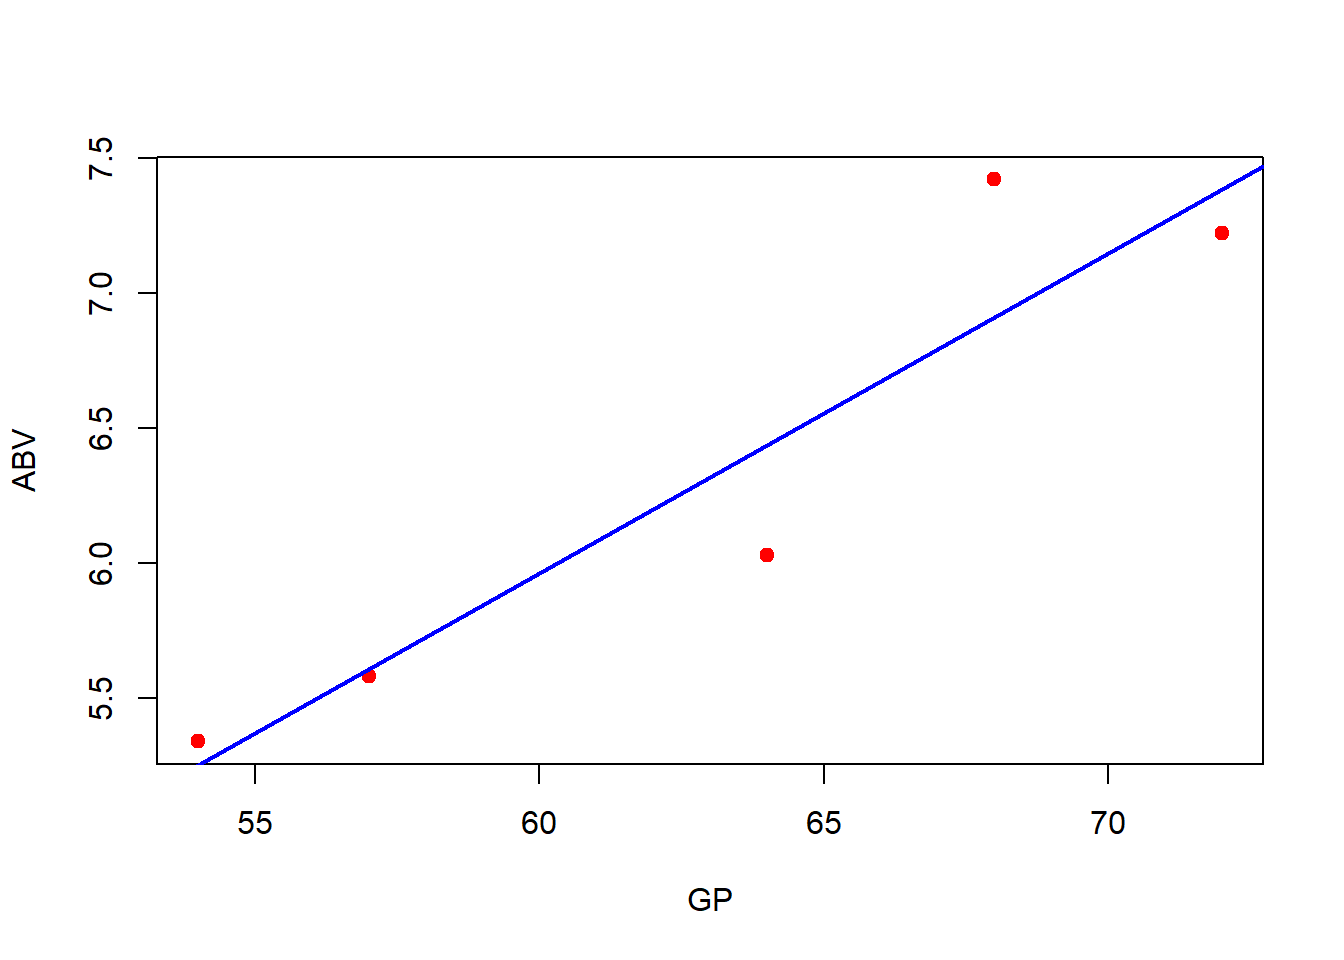
\includegraphics[width=0.75\linewidth]{_main_files/figure-latex/pabv-1} 

}

\caption{Percent ABV as a function of Gravity Points}\label{fig:pabv}
\end{figure}

Here we apply the \texttt{lm} function on the \texttt{mtcars} data frame, with weight as the independent variable and fuel economy as the dependent variable.

\begin{Shaded}
\begin{Highlighting}[]
\NormalTok{mtfit }\OtherTok{\textless{}{-}} \FunctionTok{lm}\NormalTok{(mpg}\SpecialCharTok{\textasciitilde{}}\NormalTok{wt, }\AttributeTok{data =}\NormalTok{ mtcars)}
\FunctionTok{summary}\NormalTok{(mtfit)}
\end{Highlighting}
\end{Shaded}

\begin{verbatim}
## 
## Call:
## lm(formula = mpg ~ wt, data = mtcars)
## 
## Residuals:
##     Min      1Q  Median      3Q     Max 
## -4.5432 -2.3647 -0.1252  1.4096  6.8727 
## 
## Coefficients:
##             Estimate Std. Error t value Pr(>|t|)    
## (Intercept)  37.2851     1.8776  19.858  < 2e-16 ***
## wt           -5.3445     0.5591  -9.559 1.29e-10 ***
## ---
## Signif. codes:  0 '***' 0.001 '**' 0.01 '*' 0.05 '.' 0.1 ' ' 1
## 
## Residual standard error: 3.046 on 30 degrees of freedom
## Multiple R-squared:  0.7528, Adjusted R-squared:  0.7446 
## F-statistic: 91.38 on 1 and 30 DF,  p-value: 1.294e-10
\end{verbatim}

The formula is \(\text{mpg}=37.2851-5.3445\text{wt}.\) The weight is given in 1000 pounds, so the formula says that for each additional 1000 pounds in weight, the predicted mpg \emph{decreases} by 5.3445.

We can also get the scatterplot (Fig. \ref{fig:mpgscatter}).

\begin{Shaded}
\begin{Highlighting}[]
\FunctionTok{plot}\NormalTok{(mpg}\SpecialCharTok{\textasciitilde{}}\NormalTok{wt, }\AttributeTok{data =}\NormalTok{ mtcars, }\AttributeTok{pch =} \DecValTok{19}\NormalTok{, }\AttributeTok{col =} \StringTok{"red"}\NormalTok{)}
\FunctionTok{abline}\NormalTok{(mtfit, }\AttributeTok{col =} \StringTok{"blue"}\NormalTok{, }\AttributeTok{lwd =} \DecValTok{2}\NormalTok{)}
\end{Highlighting}
\end{Shaded}

\begin{figure}

{\centering 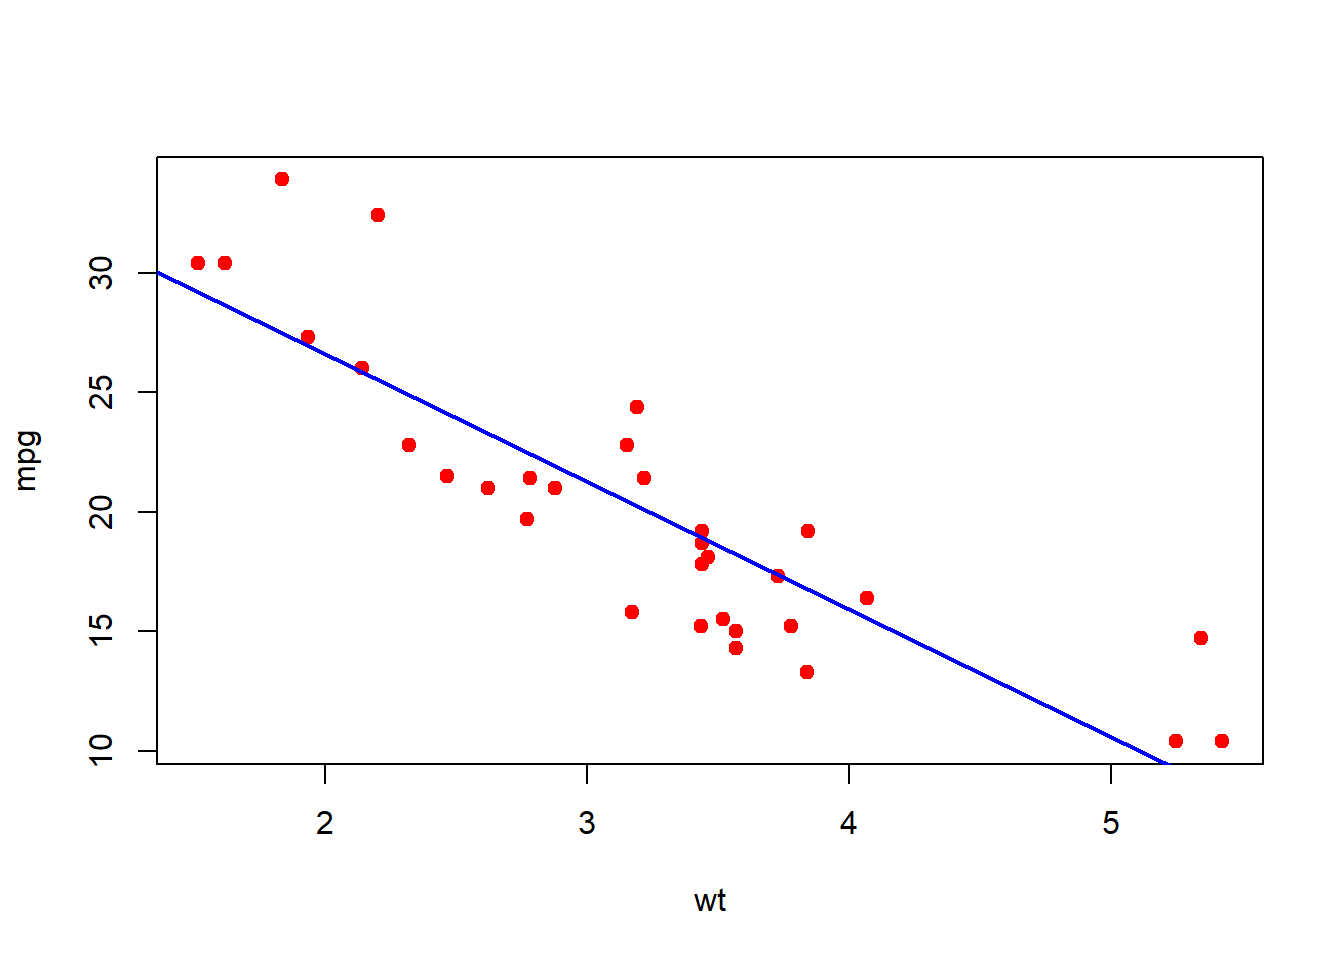
\includegraphics[width=0.75\linewidth]{_main_files/figure-latex/mpgscatter-1} 

}

\caption{Miles per gallon as a function of weight in 1000 pounds}\label{fig:mpgscatter}
\end{figure}

\subsection*{The coefficient of determination}\label{the-coefficient-of-determination}
\addcontentsline{toc}{subsection}{The coefficient of determination}

The deviation of the \(y\) values from the mean can be broken down into two pieces: the part explained by the model (\(\hat{y}_i-\bar{y}\)), and the part that is not explained (\(y_i-\hat{y}_i=e_i\)) (Fig. \ref{fig:explained}).

\begin{figure}

{\centering 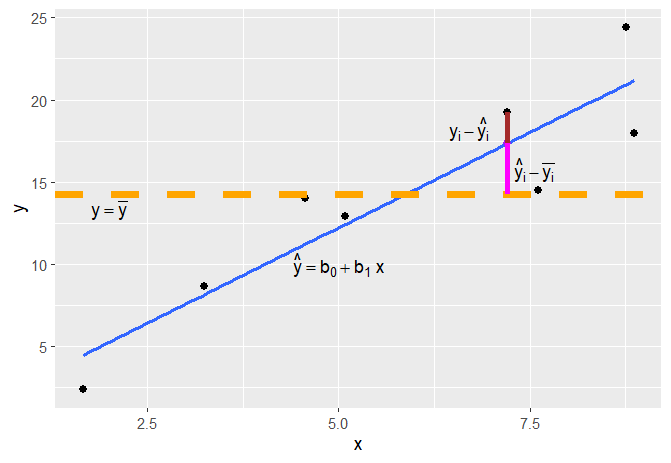
\includegraphics[width=0.75\linewidth]{images/variation} 

}

\caption{The parts of the variation in $y$}\label{fig:explained}
\end{figure}

For each observation \((x_i,y_i),\)

\[y_i-\bar{y}=(y_i-\hat{y}_i)+(\hat{y}_i-\bar{y}).\]

What's not obvious, but is true, is that if we square each term and add them up, we still have equality.

\begin{equation}
\sum_{i=1}^n (y_i-\bar{y})^2=\sum_{i=1}^n(y_i-\hat{y}_i)^2+\sum_{i=1}^n (\hat{y}_i-\bar{y})^2.
\label{eq:AnovaIdentity}
\end{equation}

This can be written as \(SST=SSE+SSR,\) where \(SST\) is the total sum of squares, \(SSE\) is the sum of squares of the error (the residuals), and \(SSR\) is the sum of squares from the regression. Rearranging the equation gives us

\[SSR=SST-SSE,\]

and dividing both sides by \(SST\) gives us

\[R^2\overset{\mathrm{def}}{=}\frac{SSR}{SST}=1-\frac{SSE}{SST}.\]

The \emph{coefficient of determination}\index{Coefficient of determination}, \(R^2,\) is the fraction of the total squared variation that comes from the regression. (I.e. the fraction that is explained.)

We don't need to mess around with \(SST\) and the others because we have the following formula for \(R^2.\)

\[R^2=r^2\]

In simple linear regression , the coefficient of determination is simply Pearson's correlation coefficient squared.

\begin{examplebox}

\begin{example}
We saw in Section \ref{CorSec} that the correlation between \texttt{mpg} and \texttt{wt} from the \texttt{mtcars} data frame is -0.8676594. That means that \(r^2=0.753\) or around 75\% of the variance in mpg can be explained by the regression equation involving weight.
\end{example}

\end{examplebox}

The coefficient of determination shows up in the R summary as \texttt{Multiple\ R-Squared}. (We will see \texttt{Adjusted\ R-Squared} in the future.)

\begin{verbatim}
## 
## Call:
## lm(formula = ABV ~ GP)
## 
## Residuals:
##        1        2        3        4        5 
##  0.50892 -0.40662 -0.02630 -0.16554  0.08954 
## 
## Coefficients:
##             Estimate Std. Error t value Pr(>|t|)  
## (Intercept) -1.15481    1.65838  -0.696   0.5363  
## GP           0.11862    0.02618   4.531   0.0201 *
## ---
## Signif. codes:  0 '***' 0.001 '**' 0.01 '*' 0.05 '.' 0.1 ' ' 1
## 
## Residual standard error: 0.3918 on 3 degrees of freedom
## Multiple R-squared:  0.8725, Adjusted R-squared:   0.83 
## F-statistic: 20.53 on 1 and 3 DF,  p-value: 0.02011
\end{verbatim}

In the GP/ABV example, the coefficient of determination is 0.8725, so around 87.25\% of the variance in ABV is explained by the equation.

\section{Uncertainty in Least Squares}\label{uncertainty-in-least-squares}

In both the matrix approach and the calculus approach to least squares, we are minimizing the same thing: the sum of squares of the residuals.

\begin{equation*}
\sum_{i=1}^n(y_i-\hat{y}_i)^2=\sum_{i=1}^n(y_i-(b_0+b_1x_i))^2
\end{equation*}

A more statistical/probabilistic approach involves what is called a \emph{linear model}\index{Linear model}. In this linear model, the underlying assumption is that the relationship between the \(x\) and \(y\) values is indeed linear, and any departure from linearity is due to randomness. The model is, for \(i=1\dots n\),

\[y_i=b_0+b_1x_i+\varepsilon_i,\]

where \((x_i,y_i)\) is the \(i\)th pair, and \(\varepsilon_i\) is the error term.

In order to estimate \(b_0\) and \(b_1\) using the observed \((x_i,y_i)\) pairs, we make some assumptions on the error terms \autocite{Navidi}.

\begin{propbox}

\textbf{Assumptions on the error terms}

In the simplest situation, the following assumptions are satisfied.

\begin{enumerate}
\def\labelenumi{\arabic{enumi}.}
\item
  The errors \(\varepsilon_1,\dots,\varepsilon_n\) are random and independent. In particular, the magnitude of any error \(\varepsilon_i\) does not influence the value of the next error.
\item
  The errors \(\varepsilon_1,\dots,\varepsilon_n\) all have mean 0.
\item
  The errors \(\varepsilon_1,\dots,\varepsilon_n\) all have the same variance, which we denote by \(\sigma^2\).
\item
  The errors \(\varepsilon_1,\dots,\varepsilon_n\) are normally distributed.
\end{enumerate}

\end{propbox}

With the assumptions in place, we can find what are called \emph{maximum likelihood estimators}, \(\hat{b}_0\) and \(\hat{b}_1\), of the true intercept and slope, \(b_0\) and \(b_1\), respectively, based on the observed data. It turns out that the normality assumption on the errors leads to the same estimates \(\hat{b}_0\) and \(\hat{b}_1\) as the linear algebra and calculus approaches!

One benefit of the linear model approach is that it allows us to estimate the uncertainty in the coefficients and in predictions based on the estimates. Let's revisit the output from our attempt to write \texttt{mpg} as a function of \texttt{wt} using the \texttt{mtcars} data frame.

\begin{Shaded}
\begin{Highlighting}[]
\NormalTok{fit }\OtherTok{\textless{}{-}} \FunctionTok{lm}\NormalTok{(mpg}\SpecialCharTok{\textasciitilde{}}\NormalTok{wt, }\AttributeTok{data =}\NormalTok{ mtcars)}
\FunctionTok{summary}\NormalTok{(fit)}\SpecialCharTok{$}\NormalTok{coefficients}
\end{Highlighting}
\end{Shaded}

\begin{verbatim}
##              Estimate Std. Error   t value     Pr(>|t|)
## (Intercept) 37.285126   1.877627 19.857575 8.241799e-19
## wt          -5.344472   0.559101 -9.559044 1.293959e-10
\end{verbatim}

The \emph{standard error}\index{Standard error} (\texttt{Std.\ Error}) of the coefficients is related to how much uncertainty there is in them. Consult a statistics textbook \autocite{OA,Navidi} for a detailed explanation of how to calculate them.

When you divide the coefficient estimates by their standard errors, the resulting value follows what is known as \emph{Student's t distribution} with \(n-2\) degrees of freedom, where \(n\) is the number of pairs in the data. In the \texttt{mtcars} data frame, there are 32 cars, so there are 30 degrees of freedom. The value in the \texttt{t\ value} column is this \(t\)-distribution number.

One question to ask is, ``Are the slope and intercept significantly different from 0?'' The values in the \texttt{Pr(\textgreater{}\textbar{}t\textbar{})} column tell us the probability of seeing values at least as extreme as they are if they were truly zero. These probabilities are called \emph{P-values}\index{P-values@{$P$-value}}. In both cases, it is extremely unlikely that they are zero. If the slope were not significantly different from 0, then the independent variable wouldn't have any significant effect on the dependent variable. We commonly consider \(P\)-values below 0.05 to be significant.

You can also use the standard error values to find confidence interval estimates\index{Confidence interval!for a coefficient} for the true values of \(b_0\) and \(b_1\). The R function \texttt{confint} applied to the \texttt{lm} output will produce these intervals.

\begin{Shaded}
\begin{Highlighting}[]
\FunctionTok{confint}\NormalTok{(fit, }\AttributeTok{level =} \FloatTok{0.95}\NormalTok{)}
\end{Highlighting}
\end{Shaded}

\begin{verbatim}
##                 2.5 %    97.5 %
## (Intercept) 33.450500 41.119753
## wt          -6.486308 -4.202635
\end{verbatim}

The numbers in the \texttt{2.5\ \%} column are the lower bounds for 95\% confidence intervals for the intercept and slope (\texttt{wt}). The numbers in the \texttt{97.5\ \%} column are the upper bounds. Note that 95\% (\texttt{level\ =\ 0.95}) is the default setting and doesn't need to be there if you are happy with that level.

\subsection*{Confidence and prediction intervals for responses}\label{confidence-and-prediction-intervals-for-responses}
\addcontentsline{toc}{subsection}{Confidence and prediction intervals for responses}

With the linear model approach, the value

\[\hat{y}=\hat{b}_0+\hat{b}_1x\]

can be thought of as the \emph{estimated mean output for a given input} \(x\). We can construct a confidence interval\index{Confidence interval!for the mean response} for the true mean response.

We can also produce what is called a \emph{prediction interval}:\index{Prediction interval} given an input \(x\), what is the likely range of \(y\) values? The \texttt{predict} function applied to the output of the \texttt{lm} function can calculate both of these intervals. To use it, we need to create a data frame with new values. (The \texttt{interval} setting will accept abbreviations of ``confidence'' and ``prediction''.)

\begin{Shaded}
\begin{Highlighting}[]
\FunctionTok{predict}\NormalTok{(fit, }\AttributeTok{newdata =} \FunctionTok{data.frame}\NormalTok{(}\AttributeTok{wt =} \DecValTok{2}\NormalTok{), }\AttributeTok{interval =} \StringTok{"conf"}\NormalTok{)}
\end{Highlighting}
\end{Shaded}

\begin{verbatim}
##        fit      lwr      upr
## 1 26.59618 24.82389 28.36848
\end{verbatim}

\begin{Shaded}
\begin{Highlighting}[]
\FunctionTok{predict}\NormalTok{(fit, }\AttributeTok{newdata =} \FunctionTok{data.frame}\NormalTok{(}\AttributeTok{wt =} \DecValTok{2}\NormalTok{), }\AttributeTok{interval =} \StringTok{"predict"}\NormalTok{)}
\end{Highlighting}
\end{Shaded}

\begin{verbatim}
##        fit      lwr      upr
## 1 26.59618 20.12811 33.06425
\end{verbatim}

These are 95\% confidence and prediction intervals, respectively, for a 2000-lb vehicle (\texttt{wt\ =\ 2}). The prediction interval is much wider, since it's giving a range of all likely values and not just the mean. The value under \texttt{fit} is what you get when you plug \texttt{wt\ =\ 2} into the regression formula.

It is fairly common to see 95\% confidence intervals for the mean response included in regression plots. Here is how to get it using the \texttt{ggplot2} package (\ref{fig:gglm}).

\begin{Shaded}
\begin{Highlighting}[]
\FunctionTok{library}\NormalTok{(ggplot2)}
\NormalTok{mtplot }\OtherTok{\textless{}{-}} \FunctionTok{ggplot}\NormalTok{(mtcars, }\FunctionTok{aes}\NormalTok{(wt,mpg)) }\SpecialCharTok{+} \FunctionTok{geom\_point}\NormalTok{() }\SpecialCharTok{+}  
          \FunctionTok{geom\_smooth}\NormalTok{(}\AttributeTok{method =} \StringTok{\textquotesingle{}lm\textquotesingle{}}\NormalTok{)}
\NormalTok{mtplot}
\end{Highlighting}
\end{Shaded}

\begin{figure}

{\centering \includegraphics[width=0.75\linewidth]{_main_files/figure-latex/gglm-1} 

}

\caption{A regression plot with confidence interval}\label{fig:gglm}
\end{figure}

It takes a little more work to include a prediction interval. Figure \ref{fig:beerpi} shows the 95\% confidence interval (gray shaded region) and 95\% prediction interval (dashed) from the GP/ABV data in Example \ref{exm:gravity}.

\begin{figure}

{\centering \includegraphics[width=0.75\linewidth]{images/beerpi} 

}

\caption{Confidence and prediction intervals}\label{fig:beerpi}
\end{figure}

\subsection*{Checking assumptions}\label{checking-assumptions}
\addcontentsline{toc}{subsection}{Checking assumptions}

A \emph{residual plot}\index{Residual plot} is a plot of residuals in a linear fit versus either the \(x\) values or the predicted \(y\) values. It can be used to see if the equal variance assumption is met. It can also display any nonlinear trend in the data.

In Figure \ref{fig:resnl}, the linear fit on the left looks pretty good, but the residual plot on the right reveals a distinct nonlinear trend.

\begin{figure}

{\centering \includegraphics[width=0.4\linewidth]{images/rp1} \includegraphics[width=0.4\linewidth]{images/rp1a} 

}

\caption{A nonlinear trend}\label{fig:resnl}
\end{figure}

In Figure \ref{fig:uneqvar}, the residual plot on the right shows that the residuals tend to spread out as \(y\) increases. This indicates that the equal variance assumption is not true.

\begin{figure}

{\centering \includegraphics[width=0.4\linewidth]{images/rp2} \includegraphics[width=0.4\linewidth]{images/rp2a} 

}

\caption{Increasing residuals}\label{fig:uneqvar}
\end{figure}

In Figure \ref{fig:assumptionsmet}, there is no obvious nonlinear trend and they seem to be fairly uniform across the board.

\begin{figure}

{\centering \includegraphics[width=0.4\linewidth]{images/rp3} \includegraphics[width=0.4\linewidth]{images/rp3a} 

}

\caption{A good looking residual plot}\label{fig:assumptionsmet}
\end{figure}

If you apply the \texttt{plot} function to the output from \texttt{lm}, you get a sequence of diagnostic plots. The first is the residual plot.

\begin{Shaded}
\begin{Highlighting}[]
\FunctionTok{par}\NormalTok{(}\AttributeTok{mfrow =} \FunctionTok{c}\NormalTok{(}\DecValTok{2}\NormalTok{,}\DecValTok{2}\NormalTok{))}
\FunctionTok{plot}\NormalTok{(fit)}
\end{Highlighting}
\end{Shaded}

\begin{figure}

{\centering \includegraphics{_main_files/figure-latex/diag-1} 

}

\caption{Diagnostic plots}\label{fig:diag}
\end{figure}

See \href{https://www.statology.org/diagnostic-plots-in-r/}{www.statology.org} \autocite{statology} for a detailed discussion of all four plots.

\section{Multilinear Regression}\label{multilinear-regression-1}

In the real world, many quantities depend on more than one independent variable. For instance, the fuel efficiency of a car might depend on its weight and on its horsepower. If the relationship is linear, we can use multilinear regression\index{Regression!multilinear} to investigate it.

We saw a short example in Section \ref{LSRSec}. Now we will develop the idea in a little more depth. Suppose that a quantity \(z\) is a linear function of \(x\) and \(y\), i.e.

\[z=b_0+b_1x+b_2y.\]

Further suppose that we have a bunch of \((x,y,z)\) data:

\[(x_1,y_1,z_1),(x_2,y_2,z_2),\dots,(x_n,y_n,z_n).\]

We'd like to use this data to find the coefficients that best fit the data. We already have the tools to do this in the least squares sense. Our data gives us \(n\) equations

\begin{align*}
    b_0+b_1x_1+b_2y_1&=z_1\\
    b_0+b_1x_2+b_2y_2&=z_2\\
    &\vdots\\
    b_0+b_1x_n+b_2y_n&=z_n.
\end{align*}

We can write this system in matrix form

\[\begin{bmatrix}1 & x_1 & y_1\\1 & x_2 & y_2\\ \vdots & \vdots & \vdots \\
1 & x_n & y_n\end{bmatrix}\begin{bmatrix}b_0\\b_1\\b_2\end{bmatrix}=\begin{bmatrix}z_1\\z_2\\ \vdots \\ z_n\end{bmatrix}\]

or

\[\mathbf{X}\mathbf{b}=\mathbf{z}.\]

Usually the system won't have a solution, but we can find a least squares approximation using the normal equations:

\[\mathbf{X}^T\mathbf{X}\mathbf{b}=\mathbf{X}^T\mathbf{z},\]

which will have a solution \(\hat{\mathbf{b}}\). It will be unique if the columns of \(\mathbf{X}\) are independent.

\begin{examplebox}

\begin{example}
Let's find the least squares equation \(\hat{z}=\hat{b}_0+\hat{b}_1x+\hat{b}_2 y\) that best fits the points in \((x,y,z)\) form: \((1,1,1),(2,0,2),(-1,-1,1),\) and \((1,1,3).\) The matrix equation is

\[\begin{bmatrix}
1 & 1 & 1 \\
1 & 2 & 0 \\
1 & -1 & -1 \\
1 & 1 & 1
\end{bmatrix}\mathbf{b}=
\begin{bmatrix}
1\\2\\1\\3
\end{bmatrix}.\]

The first column of \(\mathbf{X}\) is all 1's, the second column is the \(x\) values, and the third is the \(y\) values. The normal equation(s) are

\[\begin{bmatrix}
4 & 3 & 1\\3 & 7 & 3\\1 & 3 & 3
\end{bmatrix}\mathbf{b}=\begin{bmatrix}
7\\7\\3
\end{bmatrix}
 .\]

The least squares solution is \(\hat{\mathbf{b}}=(\mathbf{X}^T\mathbf{X})^{-1}(\mathbf{X}^T\mathbf{z})=\begin{bmatrix}
3/2\\1/4\\1/4
\end{bmatrix}\), so the equation is

\[\hat{z}=\frac{3}{2}+\frac{1}{4}x+\frac{1}{4}y.\]

The beauty of the linear algebra approach is that we can use as many independent variables as we want and the theory stays the same. The matrices involved get bigger, and it's harder to do by hand, but that's what computers are for.
\end{example}

\end{examplebox}

\subsection*{R and multilinear regression}\label{r-and-multilinear-regression}
\addcontentsline{toc}{subsection}{R and multilinear regression}

\begin{examplebox}

\begin{example}
Let's use R to find a model for \texttt{mpg} as a linear function of \texttt{wt} and \texttt{hp} from the \texttt{mtcars} data frame. We again use the \texttt{lm} function, with a plus sign separating the independent variables.

\begin{Shaded}
\begin{Highlighting}[]
\NormalTok{fit2 }\OtherTok{\textless{}{-}} \FunctionTok{lm}\NormalTok{(mpg}\SpecialCharTok{\textasciitilde{}}\NormalTok{wt}\SpecialCharTok{+}\NormalTok{hp, }\AttributeTok{data =}\NormalTok{ mtcars)}
\FunctionTok{summary}\NormalTok{(fit2)}
\end{Highlighting}
\end{Shaded}

\begin{verbatim}
## 
## Call:
## lm(formula = mpg ~ wt + hp, data = mtcars)
## 
## Residuals:
##    Min     1Q Median     3Q    Max 
## -3.941 -1.600 -0.182  1.050  5.854 
## 
## Coefficients:
##             Estimate Std. Error t value Pr(>|t|)    
## (Intercept) 37.22727    1.59879  23.285  < 2e-16 ***
## wt          -3.87783    0.63273  -6.129 1.12e-06 ***
## hp          -0.03177    0.00903  -3.519  0.00145 ** 
## ---
## Signif. codes:  0 '***' 0.001 '**' 0.01 '*' 0.05 '.' 0.1 ' ' 1
## 
## Residual standard error: 2.593 on 29 degrees of freedom
## Multiple R-squared:  0.8268, Adjusted R-squared:  0.8148 
## F-statistic: 69.21 on 2 and 29 DF,  p-value: 9.109e-12
\end{verbatim}

The coefficients appear in the Estimate column. Our model is

\[\texttt{mpg}=37.227-3.878\texttt{wt}-0.032\texttt{hp}.\]

We can use the model to estimate the \texttt{mpg} for various \texttt{wt}-\texttt{hp} pairs. For instance, a 2500-lb car with a 175-hp engine would on average get

\[\texttt{mpg}=37.227-3.878\cdot 2.5-0.032\cdot 175=21.932 \text{ miles per gallon}.\]

We can also use the predict function.

\begin{Shaded}
\begin{Highlighting}[]
\FunctionTok{predict}\NormalTok{(fit2, }\AttributeTok{newdata =} \FunctionTok{data.frame}\NormalTok{(}\AttributeTok{wt =} \FloatTok{2.5}\NormalTok{, }\AttributeTok{hp =} \DecValTok{175}\NormalTok{))}
\end{Highlighting}
\end{Shaded}

\begin{verbatim}
##        1 
## 21.97243
\end{verbatim}

The discrepancies between the two answers are due to the rounding of the coefficients. What about the rest of the output? The intercept, the \texttt{wt} coefficient, and the \texttt{hp} coefficient are all significantly different from 0. Note that we lose an additional degree of freedom when we add a variable.

The model from last section, that only had weight as a predictor, had a coefficient of determination of 0.7528. Now it's 0.8268. \emph{It will always increase when additional variables are added.} The adjusted \(R^2\) of 0.8148 is the appropriate value for comparing multiple regression models. (We'll talk about Adjusted \(R^2\) in the next section.)

In simple linear regression, the \(P\)-value associated with the \(F\) statistic\index{F statistic @{\textit{F} statistic}} is the same as the \(P\)-value for the slope. That changes in multilinear regression. We're not going to get into the details of the \(F\) statistic here, but what we're looking for is a \(P\)-value of less than \(0.05\). Otherwise, there's basically no linear relationship.
\end{example}

\end{examplebox}

\begin{examplebox}

\begin{example}
We can add all of the other variables into the mix by using a period after the tilde.

\begin{Shaded}
\begin{Highlighting}[]
\NormalTok{fitall }\OtherTok{\textless{}{-}} \FunctionTok{lm}\NormalTok{(mpg}\SpecialCharTok{\textasciitilde{}}\NormalTok{., }\AttributeTok{data =}\NormalTok{ mtcars)}
\FunctionTok{summary}\NormalTok{(fitall)}
\end{Highlighting}
\end{Shaded}

\begin{verbatim}
## 
## Call:
## lm(formula = mpg ~ ., data = mtcars)
## 
## Residuals:
##     Min      1Q  Median      3Q     Max 
## -3.4506 -1.6044 -0.1196  1.2193  4.6271 
## 
## Coefficients:
##             Estimate Std. Error t value Pr(>|t|)  
## (Intercept) 12.30337   18.71788   0.657   0.5181  
## cyl         -0.11144    1.04502  -0.107   0.9161  
## disp         0.01334    0.01786   0.747   0.4635  
## hp          -0.02148    0.02177  -0.987   0.3350  
## drat         0.78711    1.63537   0.481   0.6353  
## wt          -3.71530    1.89441  -1.961   0.0633 .
## qsec         0.82104    0.73084   1.123   0.2739  
## vs           0.31776    2.10451   0.151   0.8814  
## am           2.52023    2.05665   1.225   0.2340  
## gear         0.65541    1.49326   0.439   0.6652  
## carb        -0.19942    0.82875  -0.241   0.8122  
## ---
## Signif. codes:  0 '***' 0.001 '**' 0.01 '*' 0.05 '.' 0.1 ' ' 1
## 
## Residual standard error: 2.65 on 21 degrees of freedom
## Multiple R-squared:  0.869,  Adjusted R-squared:  0.8066 
## F-statistic: 13.93 on 10 and 21 DF,  p-value: 3.793e-07
\end{verbatim}

But maybe we shouldn't. Only the \texttt{wt} coefficient is significantly different from 0. We'll talk about model selection next section.
\end{example}

\end{examplebox}

\subsection*{Indicator variables}\label{indicator-variables}
\addcontentsline{toc}{subsection}{Indicator variables}

We can include categorical (non-numeric) variables in linear regression through the use of \emph{indicator variables}\index{Indicator variables}. An indicator variable takes on the value 1 if the categorical variable takes on a specific value and a 0 otherwise.

For instance, in the \texttt{mtcars} data frame, the \texttt{am} (1 for manual, 0 for automatic transmission) and \texttt{vs} (0 for V-shaped engine, 1 for straight) variables are actually indicator variables.

\begin{examplebox}

\begin{example}
If we find a linear model for fuel efficiency as a function of horsepower and transmission type, we get the following.

\begin{Shaded}
\begin{Highlighting}[]
\NormalTok{fitind }\OtherTok{\textless{}{-}} \FunctionTok{lm}\NormalTok{(mpg}\SpecialCharTok{\textasciitilde{}}\NormalTok{hp}\SpecialCharTok{+}\NormalTok{am, }\AttributeTok{data =}\NormalTok{ mtcars)}
\FunctionTok{summary}\NormalTok{(fitind)}
\end{Highlighting}
\end{Shaded}

\begin{verbatim}
## 
## Call:
## lm(formula = mpg ~ hp + am, data = mtcars)
## 
## Residuals:
##     Min      1Q  Median      3Q     Max 
## -4.3843 -2.2642  0.1366  1.6968  5.8657 
## 
## Coefficients:
##              Estimate Std. Error t value Pr(>|t|)    
## (Intercept) 26.584914   1.425094  18.655  < 2e-16 ***
## hp          -0.058888   0.007857  -7.495 2.92e-08 ***
## am           5.277085   1.079541   4.888 3.46e-05 ***
## ---
## Signif. codes:  0 '***' 0.001 '**' 0.01 '*' 0.05 '.' 0.1 ' ' 1
## 
## Residual standard error: 2.909 on 29 degrees of freedom
## Multiple R-squared:  0.782,  Adjusted R-squared:  0.767 
## F-statistic: 52.02 on 2 and 29 DF,  p-value: 2.55e-10
\end{verbatim}

The model is

\[\texttt{mpg}=26.585-0.059\texttt{hp}+5.277\texttt{am}.\]

Basically, the presence of a manual transmission adds 5.277 miles per gallon to the estimated fuel efficiency. We get two regression lines: one for automatics and one for manuals (Fig. \ref{fig:indicator}).
\end{example}

\end{examplebox}

\begin{figure}

{\centering \includegraphics[width=0.75\linewidth]{images/multiint} 

}

\caption{A model with an indicator term}\label{fig:indicator}
\end{figure}

Many categorical variables take on more than two different values or \emph{levels}\index{Level!of a categorical variable}. In that case, a different indicator variable is included for each level, \emph{except one}. For instance, if the season is an important variable, there could be one indicator variable for Spring (1 if Spring, 0 otherwise), one for Summer, and one for Autumn. The final season, Winter doesn't get one, because that would make the variables dependent. Winter would be the baseline value, to which all others are compared.

\begin{examplebox}

\begin{example}
Here is a fit of the population of a state as a function of the state's area and its region. \texttt{Region} is a categorical variable. The Northeast region is treated as the baseline. The other regions get their own indicators.

\begin{Shaded}
\begin{Highlighting}[]
\NormalTok{state }\OtherTok{\textless{}{-}} \FunctionTok{data.frame}\NormalTok{(state.x77)}
\NormalTok{state}\SpecialCharTok{$}\NormalTok{Region }\OtherTok{\textless{}{-}}\NormalTok{ state.region}
\NormalTok{fitstate }\OtherTok{\textless{}{-}} \FunctionTok{lm}\NormalTok{(Population}\SpecialCharTok{\textasciitilde{}}\NormalTok{Area}\SpecialCharTok{+}\NormalTok{Region, }\AttributeTok{data =}\NormalTok{ state)}
\FunctionTok{summary}\NormalTok{(fitstate)}
\end{Highlighting}
\end{Shaded}

\begin{verbatim}
## 
## Call:
## lm(formula = Population ~ Area + Region, data = state)
## 
## Residuals:
##     Min      1Q  Median      3Q     Max 
## -5952.2 -2226.6  -858.2   713.2 18110.2 
## 
## Coefficients:
##                       Estimate Std. Error t value Pr(>|t|)    
## (Intercept)          5.352e+03  1.514e+03   3.534 0.000959 ***
## Area                 7.875e-03  8.631e-03   0.912 0.366383    
## RegionSouth         -1.574e+03  1.909e+03  -0.825 0.413931    
## RegionNorth Central -1.043e+03  2.029e+03  -0.514 0.609901    
## RegionWest          -3.496e+03  2.202e+03  -1.588 0.119327    
## ---
## Signif. codes:  0 '***' 0.001 '**' 0.01 '*' 0.05 '.' 0.1 ' ' 1
## 
## Residual standard error: 4519 on 45 degrees of freedom
## Multiple R-squared:  0.05919,    Adjusted R-squared:  -0.02444 
## F-statistic: 0.7078 on 4 and 45 DF,  p-value: 0.5908
\end{verbatim}

Note how R pastes the level of the variable onto the variable name in the output. Also note the terrible coefficient of determination. This is \emph{not} a good model.
\end{example}

\end{examplebox}

\subsection*{Fitting polynomials}\label{fitting-polynomials}
\addcontentsline{toc}{subsection}{Fitting polynomials}

We can actually use linear regression to fit polynomial\index{Polynomial fit} functions to data. For instance, what if we want to find the best fitting quadratic function

\[y=b_0+b_1x+b_2x^2\]

for a set of data? You may recall that three points (with different \(x\) values) will determine a quadratic. What if we have more than 3 points?

\begin{examplebox}

\begin{example}
Let's find the least squares best fitting quadratic that goes through the points \((1,3),(2,5),(3,6),\) and \((4,7)\).
The linear system of equations for \(y=b_0+b_1x+b_2x^2\) with this data would be

\begin{align*} 
    b_0+1b_1+1^2b_2&=3\\
    b_0+2b_1+2^2b_2&=5\\
    b_0+3b_1+3^2b_2&=6\\
    b_0+4b_1+4^2b_2&=7
\end{align*}

or in matrix form

\[\begin{bmatrix}1 & 1 & 1 \\ 1 & 2 & 4\\1 & 3 & 9\\1 & 4 & 16\end{bmatrix}\begin{bmatrix}b_0\\b_1\\b_2\end{bmatrix}=\begin{bmatrix}3\\5\\6\\7\end{bmatrix}.\]

Solving the normal equations gives us

\[\hat{y}=\frac{3}{4}+\frac{51}{20}x-\frac{1}{4}x^2.\]

To do this in R, we need to be a little careful.

\begin{Shaded}
\begin{Highlighting}[]
\NormalTok{x }\OtherTok{\textless{}{-}} \FunctionTok{c}\NormalTok{(}\DecValTok{1}\NormalTok{,}\DecValTok{2}\NormalTok{,}\DecValTok{3}\NormalTok{,}\DecValTok{4}\NormalTok{)}
\NormalTok{y }\OtherTok{\textless{}{-}} \FunctionTok{c}\NormalTok{(}\DecValTok{3}\NormalTok{,}\DecValTok{5}\NormalTok{,}\DecValTok{6}\NormalTok{,}\DecValTok{7}\NormalTok{)}
\NormalTok{fitq }\OtherTok{\textless{}{-}} \FunctionTok{lm}\NormalTok{(y}\SpecialCharTok{\textasciitilde{}}\NormalTok{x}\SpecialCharTok{+}\FunctionTok{I}\NormalTok{(x}\SpecialCharTok{\^{}}\DecValTok{2}\NormalTok{))}
\FunctionTok{summary}\NormalTok{(fitq)}
\end{Highlighting}
\end{Shaded}

\begin{verbatim}
## 
## Call:
## lm(formula = y ~ x + I(x^2))
## 
## Residuals:
##     1     2     3     4 
## -0.05  0.15 -0.15  0.05 
## 
## Coefficients:
##             Estimate Std. Error t value Pr(>|t|)
## (Intercept)   0.7500     0.6225   1.205    0.441
## x             2.5500     0.5679   4.490    0.140
## I(x^2)       -0.2500     0.1118  -2.236    0.268
## 
## Residual standard error: 0.2236 on 1 degrees of freedom
## Multiple R-squared:  0.9943, Adjusted R-squared:  0.9829 
## F-statistic:    87 on 2 and 1 DF,  p-value: 0.07559
\end{verbatim}

To use powers of a variable in a model in R, we need to wrap them in the \texttt{I} function. See the fit in Figure \ref{fig:qfit}.
\end{example}

\end{examplebox}

\begin{figure}

{\centering \includegraphics[width=0.75\linewidth]{_main_files/figure-latex/qfit-1} 

}

\caption{A quadratic fit using linear regression}\label{fig:qfit}
\end{figure}

In the last example, our design matrix looked like

\[\mathbf{X}=\begin{bmatrix} 1& x_1 & x_1^2 \\1 & x_2 & x_2^2\\ \vdots & \vdots & \vdots \\ 1 & x_n & x_n^2\end{bmatrix}.\]

We actually had functions of \(x\) in the columns. We can do this for any function. For instance, if we wanted a fit of the form

\[y=b_0 +b_1\sin x+b_2\cos x,\]

the design matrix would look like

\[\mathbf{X}=\begin{bmatrix}1 & \sin x_1 & \cos x_1\\1 & \sin x_2 & \cos x_2 \\ \vdots & \vdots & \vdots \\
1 & \sin x_n & \cos x_n\end{bmatrix}.\]

\subsection*{Interactions}\label{interactions}
\addcontentsline{toc}{subsection}{Interactions}

Let's say you want to model an individual's response to a medication. The response is going to depend on a number of things, including the dosage and the person's weight. In our previous models, the response to a change in one variable wasn't dependent on the value of the other. It's not hard to imagine, however, that the response to a change in dosage will depend on the person's weight. There is an \emph{interaction}\index{Interaction} between these two variables.

The simplest way to include an interaction between variables \(x_1\) and \(x_2\) is to include the product \(x_1 x_2\) as a separate independent variable. We then have the model

\[y=b_0+b_1 x_1+b_2 x_2+b_3 x_1 x_2.\]

Adding this new term doesn't really complicate things at all.

\begin{examplebox}

\begin{example}
The price of a diamond in U.S. Dollars is a function of many things, including its weight in carats and its depth percentage. The \texttt{ggplot2} package contains a data set with this information.

\begin{Shaded}
\begin{Highlighting}[]
\FunctionTok{library}\NormalTok{(ggplot2)}
\NormalTok{diamondfit }\OtherTok{\textless{}{-}} \FunctionTok{lm}\NormalTok{(price}\SpecialCharTok{\textasciitilde{}}\NormalTok{carat}\SpecialCharTok{*}\NormalTok{depth, }\AttributeTok{data =}\NormalTok{ diamonds)}
\FunctionTok{summary}\NormalTok{(diamondfit)}
\end{Highlighting}
\end{Shaded}

\begin{verbatim}
## 
## Call:
## lm(formula = price ~ carat * depth, data = diamonds)
## 
## Residuals:
##      Min       1Q   Median       3Q      Max 
## -15039.2   -799.3    -18.1    539.6  12666.5 
## 
## Coefficients:
##              Estimate Std. Error t value Pr(>|t|)    
## (Intercept) -7823.738    592.049 -13.215   <2e-16 ***
## carat       20742.600    567.672  36.540   <2e-16 ***
## depth          90.043      9.588   9.391   <2e-16 ***
## carat:depth  -210.075      9.187 -22.868   <2e-16 ***
## ---
## Signif. codes:  0 '***' 0.001 '**' 0.01 '*' 0.05 '.' 0.1 ' ' 1
## 
## Residual standard error: 1534 on 53936 degrees of freedom
## Multiple R-squared:  0.8521, Adjusted R-squared:  0.8521 
## F-statistic: 1.036e+05 on 3 and 53936 DF,  p-value: < 2.2e-16
\end{verbatim}

The interaction term is \texttt{carat:depth}. (If you only want the interaction term and not the individual variables, use the colon instead of the asterisk.) Our model with interaction term is

\[\texttt{price}=-7824+20743\texttt{carat}+90\texttt{depth}-210(\texttt{carat})(\texttt{depth}).\]

A diamond with a depth percentage of 60 would have a price function of

\begin{align*} 
\texttt{price}&=-7824+20743\texttt{carat}+(90)(60)-(210)(60)\texttt{carat}\\
&=(-7824+5400)+(20743-12600)\texttt{carat}\\
&=-2424+8143\texttt{carat}.
\end{align*}
\end{example}

\end{examplebox}

\begin{examplebox}

\begin{example}
When we included the \texttt{am} variable in our earlier \texttt{mpg} versus \texttt{hp} model, this had the effect of creating two models with the same slope and different intercepts. When we include an interaction term, we get something different. For this example, we will be using \texttt{wt} and \texttt{am} as the interacting terms.

\begin{Shaded}
\begin{Highlighting}[]
\NormalTok{fitam }\OtherTok{\textless{}{-}} \FunctionTok{lm}\NormalTok{(mpg}\SpecialCharTok{\textasciitilde{}}\NormalTok{wt}\SpecialCharTok{*}\NormalTok{am, }\AttributeTok{data =}\NormalTok{ mtcars)}
\FunctionTok{summary}\NormalTok{(fitam)}
\end{Highlighting}
\end{Shaded}

\begin{verbatim}
## 
## Call:
## lm(formula = mpg ~ wt * am, data = mtcars)
## 
## Residuals:
##     Min      1Q  Median      3Q     Max 
## -3.6004 -1.5446 -0.5325  0.9012  6.0909 
## 
## Coefficients:
##             Estimate Std. Error t value Pr(>|t|)    
## (Intercept)  31.4161     3.0201  10.402 4.00e-11 ***
## wt           -3.7859     0.7856  -4.819 4.55e-05 ***
## am           14.8784     4.2640   3.489  0.00162 ** 
## wt:am        -5.2984     1.4447  -3.667  0.00102 ** 
## ---
## Signif. codes:  0 '***' 0.001 '**' 0.01 '*' 0.05 '.' 0.1 ' ' 1
## 
## Residual standard error: 2.591 on 28 degrees of freedom
## Multiple R-squared:  0.833,  Adjusted R-squared:  0.8151 
## F-statistic: 46.57 on 3 and 28 DF,  p-value: 5.209e-11
\end{verbatim}

The overall model is

\[\texttt{mpg}=31.416-3.786\texttt{wt}+14.878\texttt{am}-5.298\texttt{wt}\cdot \texttt{am}.\]

We basically have two different models. For automatics, we set \(\texttt{am}=0\) and get

\[\texttt{mpg}=31.416-3.786\texttt{wt}.\]

Changing \texttt{am} to 1 will change the intercept \emph{and} the slope.

\begin{align*}
\texttt{mpg}&=31.416-3.786\texttt{wt}+14.878-5.298\texttt{wt} \\
    &=46.294-9.084\texttt{wt}.
\end{align*}

When we use the indicator variable (coerced into a factor variable) as the color in \texttt{ggplot}, we get the two separate lines (Fig. \ref{fig:aminteraction}).
\end{example}

\end{examplebox}

\begin{Shaded}
\begin{Highlighting}[]
\CommentTok{\# Change the am variable to a factor variable for ggplot2}
\NormalTok{mt2}\OtherTok{\textless{}{-}}\NormalTok{mtcars}
\NormalTok{mt2}\SpecialCharTok{$}\NormalTok{am }\OtherTok{\textless{}{-}} \FunctionTok{as.factor}\NormalTok{(mtcars}\SpecialCharTok{$}\NormalTok{am)}
\NormalTok{ginteract }\OtherTok{\textless{}{-}} \FunctionTok{ggplot}\NormalTok{(mt2, }\FunctionTok{aes}\NormalTok{(mpg, wt, }\AttributeTok{color =}\NormalTok{ am))}\SpecialCharTok{+}
        \FunctionTok{geom\_point}\NormalTok{()}\SpecialCharTok{+}
        \FunctionTok{geom\_smooth}\NormalTok{(}\AttributeTok{method=} \StringTok{"lm"}\NormalTok{)}
\NormalTok{ginteract}
\end{Highlighting}
\end{Shaded}

\begin{figure}

{\centering \includegraphics[width=0.75\linewidth]{_main_files/figure-latex/aminteraction-1} 

}

\caption{Model with a categorical variable in an interaction}\label{fig:aminteraction}
\end{figure}

\section{Model Selection}\label{model-selection}

Given a data set with many independent variables, it is tempting to choose the model that uses all of them. This might not be wise, however. Some of the variables might have nothing to do with the response. Some variables might be so closely related to others that they add nothing to the model. Some statisticians believe in the \emph{principle of parsimony} \autocite{Navidi}.

\begin{notebox}
\textbf{Principle of Parsimony}\index{Principle of parsimony}
A model should contain the smallest number of variables necessary to fit the data.

\end{notebox}

We have already observed that the value of \(R^2\) increases as the number of independent variables increases. Using \(R^2\) as a criterion for choosing the best model would therefore be in conflict with the principle of parsimony. For this reason, among others, we consider the \emph{adjusted} \(R^2\)\index{Adjusted $R^2$}.

\begin{defbox}

\begin{definition}
\[\text{Adjusted } R^2=R^2-\left(\frac{k}{n-k-1}\right)(1-R^2),
\]

where \(n\) is the number of observations and \(k\) is the number of independent variables in the model.
\end{definition}

\end{defbox}

Since we're always subtracting a positive amount from \(R^2\), the adjusted \(R^2\) value is always less than \(R^2\), though if \(n\) is large, the difference can be negligible.

In earlier sections, we developed models using the \texttt{mtcars} data frame for the fuel efficiency (\texttt{mpg}) of a car as a function of several variables.

\begin{itemize}
\tightlist
\item
  With only the variable \texttt{wt}, we had \(R^2=0.7528\). With \(n=32\) and \(k=1\),
\end{itemize}

\[\text{Adjusted } R^2=0.7528-\frac{1}{30}(1-0.7528)=0.74456.\]

\begin{itemize}
\tightlist
\item
  When the variables were horsepower and weight, we had \(R^2=0.8268\). With \(k=2\), we have \[\text{Adjusted }R^2=0.8268-\frac{2}{29}(1-0.8268)=0.8149,\]
\end{itemize}

an improvement over the single variable model.

\begin{itemize}
\tightlist
\item
  Adding displacement to the model barely changed \(R^2\), as it's still 0.8268 to 4 decimal places, but with \(k=3\), we have
\end{itemize}

\[ \text{Adjusted } R^2=0.8268-\frac{3}{28}(1-0.8268)=0.8082,\]

a decrease from our two-variable model.

There are other ways of comparing the qualities of multilinear models, including AIC (Akaike information criterion) \autocite{AIC}, and BIC (Bayesian information criterion) \autocite{BIC}. Having chosen a criterion, there are different ways of identifying the \emph{best} model.

\subsection*{Best subsets regression}\label{best-subsets-regression}
\addcontentsline{toc}{subsection}{Best subsets regression}

The \emph{best subsets regression} procedure simply compares all possible models with a given number of independent variables and selects the best one. Depending on the total number of independent variables available, this can be an inefficient procedure. The \texttt{regsubsets} function from the R package \texttt{leaps} handles best subsets regression.

\begin{examplebox}

\begin{example}
In this example, we use best subsets on the \texttt{swiss} data frame to find the best model to predict \texttt{Fertility}.

\begin{Shaded}
\begin{Highlighting}[]
\FunctionTok{library}\NormalTok{(leaps)}
\NormalTok{fitbest }\OtherTok{\textless{}{-}} \FunctionTok{regsubsets}\NormalTok{(Fertility}\SpecialCharTok{\textasciitilde{}}\NormalTok{., }\AttributeTok{data =}\NormalTok{ swiss)}
\FunctionTok{summary}\NormalTok{(fitbest)}\SpecialCharTok{$}\NormalTok{outmat}
\end{Highlighting}
\end{Shaded}

\begin{verbatim}
##          Agriculture Examination Education Catholic Infant.Mortality
## 1  ( 1 ) " "         " "         "*"       " "      " "             
## 2  ( 1 ) " "         " "         "*"       "*"      " "             
## 3  ( 1 ) " "         " "         "*"       "*"      "*"             
## 4  ( 1 ) "*"         " "         "*"       "*"      "*"             
## 5  ( 1 ) "*"         "*"         "*"       "*"      "*"
\end{verbatim}

The best one-variable model uses \texttt{Education} as the independent variable. The best two-variable model uses \texttt{Education} and \texttt{Catholic}. To find the best overall model, you can apply the plot function to the \texttt{regsubsets} output (Fig. \ref{fig:leapsplot}). The best model appears at the top. In this example, the model that includes every variable except \texttt{Examination} is the best. The default selection statistic is BIC. For BIC, the lower the better.
\end{example}

\end{examplebox}

\begin{Shaded}
\begin{Highlighting}[]
\FunctionTok{plot}\NormalTok{(fitbest)}
\end{Highlighting}
\end{Shaded}

\begin{figure}

{\centering \includegraphics[width=0.75\linewidth]{_main_files/figure-latex/leapsplot-1} 

}

\caption{A best subsets plot}\label{fig:leapsplot}
\end{figure}

\subsection*{Stepwise regression}\label{stepwise-regression}
\addcontentsline{toc}{subsection}{Stepwise regression}

A somewhat more efficient method for finding the best model is \emph{stepwise regression}\index{Stepwise Regression}. In stepwise regression, you either start with the empty model or full model. If you start with the empty model, here is a summary of the forwards regression process.

\begin{enumerate}
\def\labelenumi{\arabic{enumi}.}
\item
  Find the single variable that produces the best model.
\item
  Find the variable that, when added to the first, improves the model the most.
\item
  Repeat, until no additions will improve the situation.
\end{enumerate}

Note: it is possible that after the addition of one variable, the removal of one of the already included variables will improve the model. You can include this if desired.

Backwards regression starts with the full model and eliminates variables one-by-one. It is a little easier to perform in R. The \texttt{step} function is the function to use.

\begin{examplebox}

\begin{example}
For our stepwise regression example, we again use the \texttt{swiss} data frame.

\begin{Shaded}
\begin{Highlighting}[]
\NormalTok{fitall }\OtherTok{\textless{}{-}} \FunctionTok{lm}\NormalTok{(Fertility}\SpecialCharTok{\textasciitilde{}}\NormalTok{., }\AttributeTok{data =}\NormalTok{ swiss)}
\NormalTok{fitstep }\OtherTok{\textless{}{-}} \FunctionTok{step}\NormalTok{(fitall)}
\end{Highlighting}
\end{Shaded}

\begin{verbatim}
## Start:  AIC=190.69
## Fertility ~ Agriculture + Examination + Education + Catholic + 
##     Infant.Mortality
## 
##                    Df Sum of Sq    RSS    AIC
## - Examination       1     53.03 2158.1 189.86
## <none>                          2105.0 190.69
## - Agriculture       1    307.72 2412.8 195.10
## - Infant.Mortality  1    408.75 2513.8 197.03
## - Catholic          1    447.71 2552.8 197.75
## - Education         1   1162.56 3267.6 209.36
## 
## Step:  AIC=189.86
## Fertility ~ Agriculture + Education + Catholic + Infant.Mortality
## 
##                    Df Sum of Sq    RSS    AIC
## <none>                          2158.1 189.86
## - Agriculture       1    264.18 2422.2 193.29
## - Infant.Mortality  1    409.81 2567.9 196.03
## - Catholic          1    956.57 3114.6 205.10
## - Education         1   2249.97 4408.0 221.43
\end{verbatim}

The output shows all steps in the process. The tables show the effect of removing each variable. Removing any variable above the \texttt{\textless{}none\textgreater{}} line improves the model (based on AIC). The variable at the top (if it is above \texttt{\textless{}none\textgreater{}}) goes. In this example, \texttt{Examination} gets dropped first. After that, the process stops, because the removal of any of the other variables will make the model worse.

The \texttt{step} output includes the final model, which is handy.

\begin{Shaded}
\begin{Highlighting}[]
\FunctionTok{summary}\NormalTok{(fitstep)}
\end{Highlighting}
\end{Shaded}

\begin{verbatim}
## 
## Call:
## lm(formula = Fertility ~ Agriculture + Education + Catholic + 
##     Infant.Mortality, data = swiss)
## 
## Residuals:
##      Min       1Q   Median       3Q      Max 
## -14.6765  -6.0522   0.7514   3.1664  16.1422 
## 
## Coefficients:
##                  Estimate Std. Error t value Pr(>|t|)    
## (Intercept)      62.10131    9.60489   6.466 8.49e-08 ***
## Agriculture      -0.15462    0.06819  -2.267  0.02857 *  
## Education        -0.98026    0.14814  -6.617 5.14e-08 ***
## Catholic          0.12467    0.02889   4.315 9.50e-05 ***
## Infant.Mortality  1.07844    0.38187   2.824  0.00722 ** 
## ---
## Signif. codes:  0 '***' 0.001 '**' 0.01 '*' 0.05 '.' 0.1 ' ' 1
## 
## Residual standard error: 7.168 on 42 degrees of freedom
## Multiple R-squared:  0.6993, Adjusted R-squared:  0.6707 
## F-statistic: 24.42 on 4 and 42 DF,  p-value: 1.717e-10
\end{verbatim}

Here is the process for forwards regression. In addition to the full model, we need to create an intercept-only model.

\begin{Shaded}
\begin{Highlighting}[]
\NormalTok{fitio }\OtherTok{\textless{}{-}} \FunctionTok{lm}\NormalTok{(Fertility}\SpecialCharTok{\textasciitilde{}}\DecValTok{1}\NormalTok{, }\AttributeTok{data =}\NormalTok{ swiss)}
\NormalTok{fitallf }\OtherTok{\textless{}{-}} \FunctionTok{formula}\NormalTok{(fitall)}
\NormalTok{fitstepf }\OtherTok{\textless{}{-}} \FunctionTok{step}\NormalTok{(fitio, }\AttributeTok{direction =} \StringTok{"forward"}\NormalTok{,  }
                  \AttributeTok{scope=}\NormalTok{fitallf)}
\end{Highlighting}
\end{Shaded}

\begin{verbatim}
## Start:  AIC=238.35
## Fertility ~ 1
## 
##                    Df Sum of Sq    RSS    AIC
## + Education         1    3162.7 4015.2 213.04
## + Examination       1    2994.4 4183.6 214.97
## + Catholic          1    1543.3 5634.7 228.97
## + Infant.Mortality  1    1245.5 5932.4 231.39
## + Agriculture       1     894.8 6283.1 234.09
## <none>                          7178.0 238.34
## 
## Step:  AIC=213.04
## Fertility ~ Education
## 
##                    Df Sum of Sq    RSS    AIC
## + Catholic          1    961.07 3054.2 202.18
## + Infant.Mortality  1    891.25 3124.0 203.25
## + Examination       1    465.63 3549.6 209.25
## <none>                          4015.2 213.04
## + Agriculture       1     61.97 3953.3 214.31
## 
## Step:  AIC=202.18
## Fertility ~ Education + Catholic
## 
##                    Df Sum of Sq    RSS    AIC
## + Infant.Mortality  1    631.92 2422.2 193.29
## + Agriculture       1    486.28 2567.9 196.03
## <none>                          3054.2 202.18
## + Examination       1      2.46 3051.7 204.15
## 
## Step:  AIC=193.29
## Fertility ~ Education + Catholic + Infant.Mortality
## 
##               Df Sum of Sq    RSS    AIC
## + Agriculture  1   264.176 2158.1 189.86
## <none>                     2422.2 193.29
## + Examination  1     9.486 2412.8 195.10
## 
## Step:  AIC=189.86
## Fertility ~ Education + Catholic + Infant.Mortality + Agriculture
## 
##               Df Sum of Sq    RSS    AIC
## <none>                     2158.1 189.86
## + Examination  1    53.027 2105.0 190.69
\end{verbatim}

The output is similar. Notice the plus sign in front of the variables instead of minus signs. In this process, the variable at the top is added. \emph{Replacing ``forward'' with ``both'' allows for potential additions and subtractions.}
\end{example}

\end{examplebox}

\subsection*{Some warnings}\label{some-warnings}
\addcontentsline{toc}{subsection}{Some warnings}

Before we undertake any model selection, we should consider what we are trying to accomplish.

\begin{itemize}
\item
  Are we trying to gain some understanding of the underlying relationships between variables? Note that adding and removing variables will change the coefficients in the model, unless those variables are completely uncorrelated with the other variables.
\item
  Are we trying to make predictions with our models? Oftentimes, using too many variables can lead to overfitting, which can lead to bad predictions.
\end{itemize}

\section{Logistic Regression}\label{Logistic}

Logistic regression is frequently used to make predictions about an object's classification based upon numerical measures. Here are some examples:

\begin{enumerate}
\def\labelenumi{\arabic{enumi}.}
\item
  Can you use the number of typos in an email to tell whether or not it is spam?
\item
  Can you use a baseball player's college batting average to determine whether or not they will make it to the Major Leagues?
\end{enumerate}

Even if we can't offer a guaranteed yes or no to these questions, we can at least try to give a probability that it is one thing or another.

Let's start with a motivating example. The \texttt{Pima.tr} data frame in R contains diabetes-related data obtained from a sample of Akimel O'odham, or Pima, women. If we create a boxplot of blood glucose levels grouped by diabetes status (Fig. \ref{fig:pima1}), we see that those with diabetes tend to have a higher glucose level.

\begin{Shaded}
\begin{Highlighting}[]
\FunctionTok{library}\NormalTok{(ggplot2)}
\NormalTok{Pima }\OtherTok{\textless{}{-}}\NormalTok{ MASS}\SpecialCharTok{::}\NormalTok{Pima.tr}
\NormalTok{pimabox }\OtherTok{\textless{}{-}} \FunctionTok{ggplot}\NormalTok{(Pima, }\FunctionTok{aes}\NormalTok{(glu, }\AttributeTok{fill =}\NormalTok{ type))}\SpecialCharTok{+}\FunctionTok{geom\_boxplot}\NormalTok{()}
\NormalTok{pimabox}
\end{Highlighting}
\end{Shaded}

\begin{figure}

{\centering \includegraphics{_main_files/figure-latex/pima1-1} 

}

\caption{Blood glucose levels grouped by diabetes status}\label{fig:pima1}
\end{figure}

Can we use the glucose level to estimate the probability that an individual has diabetes? That is what \emph{logistic regression}\index{Regression!logistic} tries to do. In Figure \ref{fig:pima2}, the types \texttt{No} and \texttt{Yes} are recoded as 0 and 1. If we try to fit a straight line to the data, some bad things happen. First, it's not a very good fit, and second, if we try to use the model to estimate probabilities, we will get some negative probabilities and some that are greater than one.

\begin{figure}
\includegraphics[width=0.5\linewidth]{_main_files/figure-latex/pima2-1} \includegraphics[width=0.5\linewidth]{_main_files/figure-latex/pima2-2} \caption{A straight line fit to 0-1 data}\label{fig:pima2}
\end{figure}

If we instead try to fit a s-shaped \emph{logistic} curve to the data, we get the graph in Figure \ref{fig:pima3}. The function only takes on values between 0 and 1, so we can at least attempt to use it to estimate probabilities.

\begin{figure}

{\centering \includegraphics[width=0.75\linewidth]{_main_files/figure-latex/pima3-1} 

}

\caption{A logistic fit}\label{fig:pima3}
\end{figure}

So, how do we find the logistic curve? To get to the logistic model, we start with the \emph{odds}\index{Odds!in a logistic model}. If \(p\) is the probability of an event, we define the odds to be
\[\text{odds}=\frac{p}{1-p}.\]

Note that these are the odds \emph{in favor} of the event. In gambling, people usually give the odds \emph{against} the event, which is just the reciprocal of these odds. Probabilities are between 0 and 1, whereas odds can be any non-negative number, unless \(p=1.\) In that case, the odds are undefined.

The last step before regression involves taking the (natural) log of the odds. This gives us the \emph{logit function}\index{Logit function @{logit function}}.

\[\text{logit}(p)=\ln\left(\frac{p}{1-p}\right).\]

The logit function has a range of \((-\infty,\infty).\) We want to fit a model of the form

\[\text{logit}(p)=b_0+b_1 x,\]

but there is a little problem. In our data, the values of \(p\) we have are 0 (\texttt{type\ =\ No}) and 1 (\texttt{type\ =\ Yes}). The logit function is undefined for both of those values. Long story short, we can't use our linear regression formulas to find \(b_0\) and \(b_1.\) Software packages use algorithmic methods, such as gradient descent\index{Gradient descent}, to find \emph{maximum likelihood estimates}\index{Maximum likelihood estimates} for the coefficients.

Let's say we have the coefficients, \(b_0\) and \(b_1.\) If we solve

\[ \text{logit}(p)=\ln\frac{p}{1-p}=b_0+b_1x\]

for the odds (\(p/(1-p)\)), we get

\[\text{odds}=e^{b_0+b_1 x}=e^{b_0}({e^{b_1}})^{ x}.\]

The value \(e^{b_1}\) is the \emph{odds ratio}\index{Odds ratio}. If \(x\) increases by one unit, the odds will be multiplied by \(e^{b_1}\). If we solve the odds equation for \(p\), we get

\begin{equation}
p=\frac{e^{b_0+b_1x}}{1+e^{b_0+b_1x}}=\frac{1}{e^{-(b_0+b_1x)}+1},\label{eq:logreg}
\end{equation}

which is our logistic function.

Let's use R to find our coefficients. We use the \texttt{glm} function with \texttt{family="binomial"}. (When a \emph{function} of our response variable is a linear function of independent variables, we are in the category of \emph{generalized linear models}\index{Generalized linear models}.) We don't have to recode the Yes and No values.

\begin{Shaded}
\begin{Highlighting}[]
\NormalTok{logfit }\OtherTok{\textless{}{-}} \FunctionTok{glm}\NormalTok{(type}\SpecialCharTok{\textasciitilde{}}\NormalTok{glu, }\AttributeTok{data =}\NormalTok{ Pima, }\AttributeTok{family =} \StringTok{"binomial"}\NormalTok{)}
\FunctionTok{summary}\NormalTok{(logfit)}
\end{Highlighting}
\end{Shaded}

\begin{verbatim}
## 
## Call:
## glm(formula = type ~ glu, family = "binomial", data = Pima)
## 
## Coefficients:
##              Estimate Std. Error z value Pr(>|z|)    
## (Intercept) -5.503636   0.836077  -6.583 4.62e-11 ***
## glu          0.037784   0.006278   6.019 1.76e-09 ***
## ---
## Signif. codes:  0 '***' 0.001 '**' 0.01 '*' 0.05 '.' 0.1 ' ' 1
## 
## (Dispersion parameter for binomial family taken to be 1)
## 
##     Null deviance: 256.41  on 199  degrees of freedom
## Residual deviance: 207.37  on 198  degrees of freedom
## AIC: 211.37
## 
## Number of Fisher Scoring iterations: 4
\end{verbatim}

If we exponentiate the coefficients, we get the following.

\begin{Shaded}
\begin{Highlighting}[]
\FunctionTok{exp}\NormalTok{(logfit}\SpecialCharTok{$}\NormalTok{coefficients)}
\end{Highlighting}
\end{Shaded}

\begin{verbatim}
## (Intercept)         glu 
##  0.00407194  1.03850660
\end{verbatim}

Our odds ratio is around 1.0385, so each additional unit increase in the glucose value leads to an estimated 3.85\% increase in the \emph{odds} of having diabetes. The effect on the \emph{probability} is not constant.

The logit function (see Figure \ref{fig:pima3} for the graph) is

\[p=\frac{e^{-5.5036+0.0378\text{glu}}}{1+e^{-5.5036+0.0378\text{glu}}}.\]

The \texttt{predict} function works with \texttt{glu} output. To get probabilities, we need to set \texttt{type\ =\ "response"}.

\begin{Shaded}
\begin{Highlighting}[]
\FunctionTok{predict}\NormalTok{(logfit, }\AttributeTok{newdata =} \FunctionTok{data.frame}\NormalTok{(}\AttributeTok{glu =} \FunctionTok{c}\NormalTok{(}\DecValTok{100}\NormalTok{,}\DecValTok{200}\NormalTok{)),  }
        \AttributeTok{type =} \StringTok{"response"}\NormalTok{)}
\end{Highlighting}
\end{Shaded}

\begin{verbatim}
##         1         2 
## 0.1511944 0.8862613
\end{verbatim}

The predicted probability that a woman with a glucose value of 100 has diabetes is 0.151, while a woman with a value of 200 has a probability of 0.886.

What about the other output? The standard error, \(z\)-value, and \(p\)-value have similar interpretations as in the linear regression case. Both coefficients are significantly different from zero. We will talk about the null and residual deviances a little later.

\subsection*{Logistic regression with multiple independent variables}\label{logistic-regression-with-multiple-independent-variables}
\addcontentsline{toc}{subsection}{Logistic regression with multiple independent variables}

As is the case with linear regression, we can add independent variables and interactions. Let's add \texttt{age} as a second independent variable in our diabetes model.

\begin{Shaded}
\begin{Highlighting}[]
\NormalTok{logfit2 }\OtherTok{\textless{}{-}} \FunctionTok{glm}\NormalTok{(type}\SpecialCharTok{\textasciitilde{}}\NormalTok{glu}\SpecialCharTok{+}\NormalTok{age, }\AttributeTok{data =}\NormalTok{ Pima,  }
            \AttributeTok{family =} \StringTok{"binomial"}\NormalTok{)}
\FunctionTok{summary}\NormalTok{(logfit2)}
\end{Highlighting}
\end{Shaded}

\begin{verbatim}
## 
## Call:
## glm(formula = type ~ glu + age, family = "binomial", data = Pima)
## 
## Coefficients:
##              Estimate Std. Error z value Pr(>|z|)    
## (Intercept) -6.590597   0.950274  -6.935 4.05e-12 ***
## glu          0.032860   0.006375   5.155 2.54e-07 ***
## age          0.052295   0.016796   3.114  0.00185 ** 
## ---
## Signif. codes:  0 '***' 0.001 '**' 0.01 '*' 0.05 '.' 0.1 ' ' 1
## 
## (Dispersion parameter for binomial family taken to be 1)
## 
##     Null deviance: 256.41  on 199  degrees of freedom
## Residual deviance: 197.11  on 197  degrees of freedom
## AIC: 203.11
## 
## Number of Fisher Scoring iterations: 4
\end{verbatim}

All coefficients are significantly different from zero. When we exponentiate those coefficients, we get the odds ratios for both glucose and age.

\begin{Shaded}
\begin{Highlighting}[]
\FunctionTok{exp}\NormalTok{(logfit2}\SpecialCharTok{$}\NormalTok{coefficients)}
\end{Highlighting}
\end{Shaded}

\begin{verbatim}
## (Intercept)         glu         age 
##  0.00137322  1.03340625  1.05368617
\end{verbatim}

Again, we can make predictions.

\begin{Shaded}
\begin{Highlighting}[]
\NormalTok{pdata }\OtherTok{\textless{}{-}} \FunctionTok{data.frame}\NormalTok{(}\AttributeTok{glu =} \FunctionTok{c}\NormalTok{(}\DecValTok{100}\NormalTok{,}\DecValTok{200}\NormalTok{), }\AttributeTok{age =} \FunctionTok{c}\NormalTok{(}\DecValTok{20}\NormalTok{,}\DecValTok{30}\NormalTok{))}
\FunctionTok{predict}\NormalTok{(logfit2, }\AttributeTok{newdata =}\NormalTok{ pdata,  }\AttributeTok{type =} \StringTok{"response"}\NormalTok{)}
\end{Highlighting}
\end{Shaded}

\begin{verbatim}
##          1          2 
## 0.09460463 0.82495991
\end{verbatim}

\subsection*{Likelihood and deviance}\label{likelihood-and-deviance}
\addcontentsline{toc}{subsection}{Likelihood and deviance}

The diagnostic output includes null and residual deviances. Let's talk about those. First, we need to talk about the likelihood.

Suppose our \(i\)th observation is given by a pair \((x_i,y_i),\) where \(y_i\) is either 0 or 1. When we create our logistic model, we get an estimated probability \(\hat{p}_i\) that \(y=1\) given that \(x=x_i\). The \emph{likelihood} of this particular observation is then \(\hat{p}_i\) if \(y_i=1\) or \(1-\hat{p}_i\) if \(y_i=0.\) We can combine this likelihood into a single product:

\[\hat{p}_i^{y_i}(1-\hat{p}_i)^{1-y_i}.\]

If \(y_i=1,\) then the \((1-\hat{p}_i)\) exponent is 0, and similarly, when \(y_i=0,\) the \(\hat{p}_i\) exponent is 0. We assume that individual observations are independent of each other, which allows us to get a likelihood function for the whole data set by multiplying the individual likelihoods. (Assume we have \(n\) observations.) This is a function of the coefficients \(b_0\) and \(b_1\)

\[L(b_0,b_1)=\prod_{i=1}^n \hat{p}_i^{y_i}(1-\hat{p}_i)^{1-y_i},\]

where

\[p_i=\frac{e^{b_0+b_1x_i}}{1+e^{b_0+b_1x_i}}.\]

The \(\Pi\) represents a product of multiple terms much like a \(\Sigma\) represnts a sum of multiple terms.

The maximum likelihood estimates\index{Maximum likelihood estimates! in logistic regression} are the values of \(b_0\) and \(b_1\) that maximize this function. It is often easier in practice to maximize the natural logarithm of the likelihood function. Remember that the log of a product is the sum of the logs, so we have

\[\ell=\ln L=\sum_{i=1}^n\left( y_i\ln(\hat{p}_i)+(1-y_i)\ln(1-\hat{p}_i)\right).\]

For observation \(i\), the regular residual is \(e_i=y_i-\hat{p}_i.\) We then define the \emph{deviance residuals}\index{Deviance residual} to be

\[d_i=\text{sign}(e_i)\left[-2(y_i\ln(\hat{p}_i)+(1-y_i)\ln(1-\hat{p}_i))\right]^{1/2},\]

where \(\text{sign}(e_i)\) is -1 if \(e_i<0\) and 1 if \(e_i>0.\) These deviance residuals are stored in the logistic regression output.

\begin{Shaded}
\begin{Highlighting}[]
\FunctionTok{head}\NormalTok{(}\FunctionTok{residuals}\NormalTok{(logfit),}\DecValTok{4}\NormalTok{)}
\end{Highlighting}
\end{Shaded}

\begin{verbatim}
##          1          2          3          4 
## -0.4467738  0.5368785 -0.3795802 -1.4991921
\end{verbatim}

The \emph{residual deviance}\index{Deviance!residual} is then the sum of the squares of the deviance residuals.

\begin{Shaded}
\begin{Highlighting}[]
\FunctionTok{sum}\NormalTok{((}\FunctionTok{residuals}\NormalTok{(logfit))}\SpecialCharTok{\^{}}\DecValTok{2}\NormalTok{)}
\end{Highlighting}
\end{Shaded}

\begin{verbatim}
## [1] 207.3727
\end{verbatim}

\begin{Shaded}
\begin{Highlighting}[]
\FunctionTok{deviance}\NormalTok{(logfit)}
\end{Highlighting}
\end{Shaded}

\begin{verbatim}
## [1] 207.3727
\end{verbatim}

We define the \emph{null deviance}\index{Deviance!null} similarly, but we set \(\hat{p}_i=\hat{p},\) where \(\hat{p}\) is the proportion of ones (or Yesses) in the data. In our Pima data set, \(\hat{p}=68/200=0.34.\) The null model is basically an intercept-only model. If a logistic model is any good, it's residual deviance should be significantly smaller than the null deviance.

\begin{Shaded}
\begin{Highlighting}[]
\NormalTok{logfit}\SpecialCharTok{$}\NormalTok{null.deviance}
\end{Highlighting}
\end{Shaded}

\begin{verbatim}
## [1] 256.4142
\end{verbatim}

One very simple \(R^2\) analog for logistic regression is

\begin{equation}R^2=1-\frac{\text{Residual Deviance}}{\text{Null Deviance}}.
\label{eq:R2log}
\end{equation}

In our one-variable example, we have

\[R^2=1-\frac{207.37}{256.41}=0.1913.\]

When we add age as the second independent variable, we get

\[R^2=1-\frac{197.11}{256.41}=0.2313.\]

\section{Gradient Descent}\label{GDA}

In Section \ref{Logistic}, we couldn't use a formula to find the coefficient estimates. There are various approximation techniques we can use to estimate parameters. One of them is the method of \emph{gradient descent}\index{Gradient descent}, which can find minimum and maximum values of functions. This discussion does assume a working knowledge of partial differentiation, which is covered in Appendix A.

We will start with the one-variable case. Suppose we want to find the minimum value of the function

\[f(x)=x^4-3x^2+5x+10.\]

Its derivative is the cubic function

\[f'(x)=4x^3-6x+5.\]

Finding the critical number involves solving a cubic equation, which is a pain in the neck. Instead, we will be taking advantage of the geometry of the graph to estimate the critical number. From the graph (Fig. \ref{fig:GD1}), we see that the minimum value occurs between \(-2\) and \(-1.\)

\begin{figure}

{\centering \includegraphics[width=0.4\linewidth]{images/dg1} \includegraphics[width=0.4\linewidth]{images/dg2} 

}

\caption{Finding a local minimum}\label{fig:GD1}
\end{figure}

Note that to the left of the minimum, \(f'<0\), while to the right, \(f'>0\). Also, because of the continuity of \(f'\), the closer \(x\) gets to the minimum, the closer \(f'(x)\) gets to 0.

Our algorithm will start with a guess \(x_0\) that we hope is close to the critical number. The sign of \(f'(x_0)\) will tell us whether we need to move to the left or right: to the right if \(f'(x_0)<0\) and to the left if \(f'(x_0)>0\) (Fig. \ref{fig:GD2}).

\begin{figure}

{\centering \includegraphics[width=0.4\linewidth]{images/dg3} \includegraphics[width=0.4\linewidth]{images/dg4} 

}

\caption{Left or right}\label{fig:GD2}
\end{figure}

The magnitude (absolute value) of \(f'(x_0)\) tells us approximately how far we need to move. Remember that \(f'(x)\) approaches 0 as \(x\) approaches the critical number. How far we move in either direction can be adjusted by what is called the \emph{learning rate}\index{Learning rate}, which we will denote by \(\lambda\), where \(\lambda>0\). Once we settle on a learning rate, we have our iteration formula.

\begin{align*}
    x_1&=x_0-\lambda f'(x_0)\\
    x_2&=x_1-\lambda f'(x_1)\\
    &\vdots \\
    x_{n+1}&=x_n-\lambda f'(x_n).
\end{align*}

If \(f'(x_n)<0\), then, since we are subtracting \(\lambda f'(x_n)\), we will move to the right. If \(f'(x_n)>0\), we will move to the left. The larger the value of \(|f'(x_n)|\), the farther we move. We need to choose \(\lambda\) so that we don't move too far. This can involve trial and error. It also can be adjusted using a \emph{learning rate schedule} as we get closer to our critical number.

Suppose we start with an initial guess of \(x_0=-2.0\) and a learning rate of \(\lambda=0.001\) Then

\[x_1=-2.0-0.001\cdot f'(-2.0)=-2.0-0.001\cdot(-15)=-1.985.\]

Our first 5 steps look like this.

\begin{longtable}[]{@{}lr@{}}
\toprule\noalign{}
\(n\) & \(x_n\) \\
\midrule\noalign{}
\endhead
\bottomrule\noalign{}
\endlastfoot
\(0\) & \(-2.0\) \\
\(1\) & \(-1.985\) \\
\(2\) & \(-1.9706\) \\
\(3\) & \(-1.9568\) \\
\(4\) & \(-1.9436\) \\
\(5\) & \(-1.9309\) \\
\end{longtable}

If we look at the \((x_n,f(x_n))\)-pairs on the graph (Fig. \ref{fig:GD3}), we see that we are making slow, but steady progress.

\begin{figure}

{\centering \includegraphics[width=0.75\linewidth]{images/gd1} 

}

\caption{Gradient descent}\label{fig:GD3}
\end{figure}

Our gradient descent algorithm needs a mechanism for deciding when we're close enough. We can choose to terminate the process when consecutive \(x\) values agree within a certain amount, or perhaps when the absolute value of \(f'(x_n)\) gets below a certain amount. We should also set a maximum number of iterations that we want to go through, just in case there is a problem. Here is our algorithm.

\begin{Shaded}
\begin{Highlighting}[]
\CommentTok{\# Define f and f\textquotesingle{}}
\NormalTok{f }\OtherTok{\textless{}{-}} \ControlFlowTok{function}\NormalTok{(x) x}\SpecialCharTok{\^{}}\DecValTok{4{-}3}\SpecialCharTok{*}\NormalTok{x}\SpecialCharTok{\^{}}\DecValTok{2}\SpecialCharTok{+}\DecValTok{5}\SpecialCharTok{*}\NormalTok{x}\SpecialCharTok{+}\DecValTok{10}
\NormalTok{df }\OtherTok{\textless{}{-}} \ControlFlowTok{function}\NormalTok{(x) }\DecValTok{4}\SpecialCharTok{*}\NormalTok{x}\SpecialCharTok{\^{}}\DecValTok{3{-}6}\SpecialCharTok{*}\NormalTok{x}\SpecialCharTok{+}\DecValTok{5}

\CommentTok{\# initialization}
\NormalTok{x0 }\OtherTok{\textless{}{-}} \SpecialCharTok{{-}}\DecValTok{2} \CommentTok{\#initial guess}
\NormalTok{lambda }\OtherTok{\textless{}{-}} \FloatTok{0.001} \CommentTok{\#learning rate}
\NormalTok{tol }\OtherTok{\textless{}{-}} \FloatTok{0.0001} \CommentTok{\#tolerance (When do we stop?)}
\NormalTok{maxsteps }\OtherTok{\textless{}{-}} \DecValTok{5000}
\NormalTok{steps }\OtherTok{\textless{}{-}} \DecValTok{0}

\CommentTok{\# The iteration}
\ControlFlowTok{while}\NormalTok{(}\FunctionTok{abs}\NormalTok{(}\FunctionTok{df}\NormalTok{(x0)) }\SpecialCharTok{\textgreater{}}\NormalTok{ tol }\SpecialCharTok{\&}\NormalTok{ steps }\SpecialCharTok{\textless{}}\NormalTok{ maxsteps)\{}
\NormalTok{  x0}\OtherTok{\textless{}{-}}\NormalTok{x0}\SpecialCharTok{{-}}\NormalTok{lambda}\SpecialCharTok{*}\FunctionTok{df}\NormalTok{(}\AttributeTok{x=}\NormalTok{x0)}
\NormalTok{  steps}\OtherTok{\textless{}{-}}\NormalTok{steps}\SpecialCharTok{+}\DecValTok{1}\NormalTok{\}}

\NormalTok{c1 }\OtherTok{\textless{}{-}} \FunctionTok{paste}\NormalTok{(}\StringTok{"x = "}\NormalTok{,}\FunctionTok{round}\NormalTok{(x0,}\DecValTok{3}\NormalTok{))}
\NormalTok{c2 }\OtherTok{\textless{}{-}} \FunctionTok{paste}\NormalTok{(}\StringTok{"minimum = "}\NormalTok{,}\FunctionTok{round}\NormalTok{(}\FunctionTok{f}\NormalTok{(x0),}\DecValTok{3}\NormalTok{))}
\NormalTok{c3 }\OtherTok{\textless{}{-}} \FunctionTok{paste}\NormalTok{(}\StringTok{"steps = "}\NormalTok{, steps)}
\FunctionTok{cat}\NormalTok{(c1,c2,c3,}\AttributeTok{sep=}\StringTok{"}\SpecialCharTok{\textbackslash{}n}\StringTok{"}\NormalTok{)}
\end{Highlighting}
\end{Shaded}

\begin{verbatim}
## x =  -1.523
## minimum =  0.807
## steps =  507
\end{verbatim}

We've found the location of the minimum in a measly 507 steps. If that seems too slow, we can increase the learning rate. When the learning rate is adjusted to \(\lambda=0.01\), we get convergence in 46 steps. With \(\lambda=0.05\), it converges in six (Fig. \ref{fig:GD4})!

\begin{figure}

{\centering \includegraphics[width=0.4\linewidth]{images/gd3} \includegraphics[width=0.4\linewidth]{images/gd4} 

}

\caption{Learning rates $\lambda=0.01$ (left),$\lambda=0.05$ (right)}\label{fig:GD4}
\end{figure}

If we pick a value of \(\lambda\) that is too high, for instance, \(\lambda=0.1\), something bad happens. It just bounces around between two values (Fig. \ref{fig:GD5}).

\begin{figure}

{\centering \includegraphics[width=0.75\linewidth]{images/gd5} 

}

\caption{A learning rate that is too high}\label{fig:GD5}
\end{figure}

This function in Figure \ref{fig:GD6} has two local minima. If we start near the one on the right, and use a small enough learning rate, we converge to it. If our learning rate is too large, we end up heading to the other minimum.

\begin{figure}

{\centering \includegraphics[width=0.4\linewidth]{images/gd6} \includegraphics[width=0.4\linewidth]{images/gd7} 

}

\caption{Two local minima}\label{fig:GD6}
\end{figure}

\subsection*{Functions of several variables}\label{functions-of-several-variables}
\addcontentsline{toc}{subsection}{Functions of several variables}

Now let's turn to functions of several variables. As an example, let's try to find the minimum value of

\[f(x,y)=x^4+y^4-x+2y.\]

The 3D and contour plots for \(f\) appear in Figure \ref{fig:GD7}.

\begin{figure}

{\centering \includegraphics[width=0.4\linewidth]{images/gd8} \includegraphics[width=0.4\linewidth]{images/gd9} 

}

\caption{A function of two variables.}\label{fig:GD7}
\end{figure}

Recall that at every point \((x,y)\), the gradient of \(f\), \(\nabla f(x,y)\), points in the direction of greatest increase (Fig. \ref{fig:GD8}). If we want to find the minimum of \(f\), we need to go in the opposite direction.

\begin{figure}

{\centering \includegraphics[width=0.5\linewidth]{images/gd10} 

}

\caption{The gradient points uphill}\label{fig:GD8}
\end{figure}

If our initial guess in vector form is \(\begin{bmatrix}x_0\\y_0\end{bmatrix}\), then our iteration formula is

\[\begin{bmatrix}x_{n+1}\\y_{n+1}\end{bmatrix}=\begin{bmatrix}x_{n}\\y_{n}\end{bmatrix}-\lambda \nabla f(x_n,y_n).\]

The process can either terminate when successive approximations get to be within a certain amount of each other, or when the norm of \(\nabla f(x_n,y_n)\) gets below a certain value. It can also terminate if it takes too long to converge.

With our example, \(f(x,y)=x^4+y^4-x+2y\), we have

\[\nabla f(x,y)=\begin{bmatrix}4x^3-1\\4y^3+2\end{bmatrix}.\]

Choosing an initial guess of \((x_0,y_0)=(0,0)\), and \(\lambda=0.01\), our next step is

\[\begin{bmatrix} x_1\\y_1\end{bmatrix}=\begin{bmatrix}0\\0\end{bmatrix}-0.01\left[\begin{array}{r}-1\\2\end{array}\right]=\left[\begin{array}{r}0.01\\-0.02\end{array}\right].\]

Here is the algorithm in R.

\begin{Shaded}
\begin{Highlighting}[]
\CommentTok{\# Define the functions and partial derivatives}
\NormalTok{f}\OtherTok{\textless{}{-}}\ControlFlowTok{function}\NormalTok{(x,y) x}\SpecialCharTok{\^{}}\DecValTok{4}\SpecialCharTok{+}\NormalTok{y}\SpecialCharTok{\^{}}\DecValTok{4}\SpecialCharTok{{-}}\NormalTok{x}\SpecialCharTok{+}\DecValTok{2}\SpecialCharTok{*}\NormalTok{y}
\NormalTok{fx}\OtherTok{\textless{}{-}}\ControlFlowTok{function}\NormalTok{(x,y) }\DecValTok{4}\SpecialCharTok{*}\NormalTok{x}\SpecialCharTok{\^{}}\DecValTok{3{-}1}
\NormalTok{fy}\OtherTok{\textless{}{-}}\ControlFlowTok{function}\NormalTok{(x,y) }\DecValTok{4}\SpecialCharTok{*}\NormalTok{y}\SpecialCharTok{\^{}}\DecValTok{3}\SpecialCharTok{+}\DecValTok{2}

\CommentTok{\# Initialize with (x0,y0)=(0,0)}
\NormalTok{x0 }\OtherTok{\textless{}{-}} \DecValTok{0}
\NormalTok{y0 }\OtherTok{\textless{}{-}} \DecValTok{0}
\NormalTok{lambda }\OtherTok{\textless{}{-}} \FloatTok{0.01}
\NormalTok{maxsteps }\OtherTok{\textless{}{-}} \DecValTok{5000}
\NormalTok{steps }\OtherTok{\textless{}{-}} \DecValTok{0}
\NormalTok{tol }\OtherTok{\textless{}{-}} \FloatTok{0.0001}

\CommentTok{\# Find the norm of the gradient at the initial point}
\NormalTok{gnorm }\OtherTok{\textless{}{-}} \FunctionTok{sqrt}\NormalTok{(}\FunctionTok{fx}\NormalTok{(x0,y0)}\SpecialCharTok{\^{}}\DecValTok{2}\SpecialCharTok{+}\FunctionTok{fy}\NormalTok{(x0,y0)}\SpecialCharTok{\^{}}\DecValTok{2}\NormalTok{)  }

\CommentTok{\# The iteration}
\ControlFlowTok{while}\NormalTok{(gnorm}\SpecialCharTok{\textgreater{}}\NormalTok{tol }\SpecialCharTok{\&}\NormalTok{ steps}\SpecialCharTok{\textless{}}\NormalTok{maxsteps)\{}
\NormalTok{  x1 }\OtherTok{\textless{}{-}}\NormalTok{ x0}\SpecialCharTok{{-}}\NormalTok{lambda}\SpecialCharTok{*}\FunctionTok{fx}\NormalTok{(x0,y0)}
\NormalTok{  y1 }\OtherTok{\textless{}{-}}\NormalTok{ y0}\SpecialCharTok{{-}}\NormalTok{lambda}\SpecialCharTok{*}\FunctionTok{fy}\NormalTok{(x0,y0)}
\NormalTok{  x0 }\OtherTok{\textless{}{-}}\NormalTok{ x1}
\NormalTok{  y0 }\OtherTok{\textless{}{-}}\NormalTok{ y1}
\NormalTok{  steps}\OtherTok{\textless{}{-}}\NormalTok{steps}\SpecialCharTok{+}\DecValTok{1}
\NormalTok{  gnorm}\OtherTok{\textless{}{-}}\FunctionTok{sqrt}\NormalTok{(}\FunctionTok{fx}\NormalTok{(x0,y0)}\SpecialCharTok{\^{}}\DecValTok{2}\SpecialCharTok{+}\FunctionTok{fy}\NormalTok{(x0,y0)}\SpecialCharTok{\^{}}\DecValTok{2}\NormalTok{)}
\NormalTok{\}}

\NormalTok{c1 }\OtherTok{\textless{}{-}} \FunctionTok{paste}\NormalTok{(}\StringTok{"(x,y) = ("}\NormalTok{,}\FunctionTok{round}\NormalTok{(x0,}\DecValTok{3}\NormalTok{),}\StringTok{","}\NormalTok{,}\FunctionTok{round}\NormalTok{(y0,}\DecValTok{3}\NormalTok{),}\StringTok{")"}\NormalTok{)}
\NormalTok{c2 }\OtherTok{\textless{}{-}} \FunctionTok{paste}\NormalTok{(}\StringTok{"minimum = "}\NormalTok{,}\FunctionTok{round}\NormalTok{(}\FunctionTok{f}\NormalTok{(x0,y0),}\DecValTok{3}\NormalTok{))}
\NormalTok{c3 }\OtherTok{\textless{}{-}} \FunctionTok{paste}\NormalTok{(}\StringTok{"steps = "}\NormalTok{, steps)}
\FunctionTok{cat}\NormalTok{(c1,c2,c3,}\AttributeTok{sep=}\StringTok{"}\SpecialCharTok{\textbackslash{}n}\StringTok{"}\NormalTok{)}
\end{Highlighting}
\end{Shaded}

\begin{verbatim}
## (x,y) = ( 0.63 , -0.794 )
## minimum =  -1.663
## steps =  243
\end{verbatim}

Figure \ref{fig:GD9} shows the path to the minimum. Of course, we can improve covergence by adjusting the learning rate.

\begin{figure}

{\centering \includegraphics[width=0.5\linewidth]{images/gd11} 

}

\caption{Gradient descent to a minimum for a function of two variables}\label{fig:GD9}
\end{figure}

\subsection*{Optimizing parameters}\label{optimizing-parameters}
\addcontentsline{toc}{subsection}{Optimizing parameters}

An important application of gradient descent algorithms is in the optimization of parameters. As a simple example, we will use it to approximate the least squares regression coefficients. The gradient descent algorithm needs a function to minimize. In least squares regression, we have a natural candidate: the sum of squares of the residuals,

\[S=\sum_{i=1}^n(y_i-(\hat{b}_0+\hat{b}_1x_i))^2,\]

which is a function of \(\hat{b}_0\) and \(\hat{b}_1\), the parameters that we are trying to estimate. We're going to adjust this a little bit.

The generic term for the function that we try to minimize in gradient descent is the \emph{cost function}\index{Cost function}. The traditional cost function for regression is

\[f(\hat{b}_0,\hat{b}_1)=\frac{1}{2n}\sum_{i=1}^n(y_i-(\hat{b}_0+\hat{b}_1x_i))^2\]

(or sometimes just \(1/n\) in front). The scaling means that the term won't grow as the sample size grows. The 2 goes away when we take the partial derivatives. Gradient descent requires the gradient, and the partial derivatives are

\[\frac{\partial f}{\partial \hat{b}_0}=-\frac{1}{n}\sum_{i=1}^n(y_i-(\hat{b}_0+\hat{b}_1x_i))\]

and

\[\frac{\partial f}{\partial \hat{b}_1}=-\frac{1}{n}\sum_{i=1}^n(y_i-(\hat{b}_0+\hat{b}_1x_i))x_i.\]

We saw the unscaled version of these when we derived the formulas for \(\hat{b}_0\) and \(\hat{b}_1\).

Let's try to use gradient descent to find \(\hat{b}_0\) and \(\hat{b}_1\) for the following data.

\begin{longtable}[]{@{}cc@{}}
\toprule\noalign{}
\(x_i\) & \(y_i\) \\
\midrule\noalign{}
\endhead
\bottomrule\noalign{}
\endlastfoot
1 & 3 \\
2 & 4 \\
3 & 2 \\
4 & 5 \\
\end{longtable}

We'll start with initial guesses of \(\hat{b}_0=2\) and \(\hat{b}_1=1\), and use a learning rate of \(\lambda=0.01\). We're going to calculate each pair's contribution to the gradient in this table.

\begin{longtable}[]{@{}
  >{\raggedright\arraybackslash}p{(\columnwidth - 6\tabcolsep) * \real{0.0737}}
  >{\raggedright\arraybackslash}p{(\columnwidth - 6\tabcolsep) * \real{0.0842}}
  >{\raggedright\arraybackslash}p{(\columnwidth - 6\tabcolsep) * \real{0.3895}}
  >{\raggedright\arraybackslash}p{(\columnwidth - 6\tabcolsep) * \real{0.4526}}@{}}
\toprule\noalign{}
\begin{minipage}[b]{\linewidth}\raggedright
\(x_i\)
\end{minipage} & \begin{minipage}[b]{\linewidth}\raggedright
\(y_i\)
\end{minipage} & \begin{minipage}[b]{\linewidth}\raggedright
\(-\frac{1}{4}(y_i-(\hat{b}_0+\hat{b}_1x_i))\)
\end{minipage} & \begin{minipage}[b]{\linewidth}\raggedright
\(-\frac{1}{4}(y_i-(\hat{b}_0+\hat{b}_1x_i))x_i\)
\end{minipage} \\
\midrule\noalign{}
\endhead
\bottomrule\noalign{}
\endlastfoot
1 & 3 & \(-\frac{1}{4}(3-(2+1\cdot 1))=0\) & \(-\frac{1}{4}(3-(2+1\cdot 1))\cdot 1=0\) \\
2 & 4 & \(-\frac{1}{4}(4-(2+1\cdot 2))=0\) & \(-\frac{1}{4}(4-(2+1\cdot 2))\cdot 2=0\) \\
3 & 2 & \(-\frac{1}{4}(2-(2+1\cdot 3))=0.75\) & \(-\frac{1}{4}(2-(2+1\cdot 3)\cdot 3=2.25\) \\
4 & 5 & \(-\frac{1}{4}(5-(2+1\cdot 4))=0.25\) & \(-\frac{1}{4}(5-(2+1\cdot 4))\cdot 4=1\) \\
& \(\sum\) & \(1\) & \(3.25\) \\
\end{longtable}

Our next guess for \(\hat{b}_0\) will be \(2-0.01\cdot 1=1.99\) and our next guess for \(\hat{b}_1\) will be \(1-0.01\cdot 3.25=0.9675\). We'll continue with R.

\begin{Shaded}
\begin{Highlighting}[]
\CommentTok{\# Cost function and its partials}
\NormalTok{cost }\OtherTok{\textless{}{-}} \ControlFlowTok{function}\NormalTok{(x,y,b0,b1)\{}
  \FunctionTok{sum}\NormalTok{((y}\SpecialCharTok{{-}}\NormalTok{(b0}\SpecialCharTok{+}\NormalTok{b1}\SpecialCharTok{*}\NormalTok{x))}\SpecialCharTok{\^{}}\DecValTok{2}\NormalTok{)}\SpecialCharTok{/}\NormalTok{(}\DecValTok{2}\SpecialCharTok{*}\FunctionTok{length}\NormalTok{(x))\}}
\NormalTok{dcostb0 }\OtherTok{\textless{}{-}} \ControlFlowTok{function}\NormalTok{(x,y,b0,b1)\{}
  \SpecialCharTok{{-}}\FunctionTok{sum}\NormalTok{(y}\SpecialCharTok{{-}}\NormalTok{(b0}\SpecialCharTok{+}\NormalTok{b1}\SpecialCharTok{*}\NormalTok{x))}\SpecialCharTok{/}\FunctionTok{length}\NormalTok{(x)\}}
\NormalTok{dcostb1 }\OtherTok{\textless{}{-}} \ControlFlowTok{function}\NormalTok{(x,y,b0,b1)\{}
  \SpecialCharTok{{-}}\FunctionTok{sum}\NormalTok{(y}\SpecialCharTok{*}\NormalTok{x}\SpecialCharTok{{-}}\NormalTok{b0}\SpecialCharTok{*}\NormalTok{x}\SpecialCharTok{{-}}\NormalTok{b1}\SpecialCharTok{*}\NormalTok{x}\SpecialCharTok{\^{}}\DecValTok{2}\NormalTok{)}\SpecialCharTok{/}\FunctionTok{length}\NormalTok{(x)\}}

\CommentTok{\# Data}
\NormalTok{x }\OtherTok{\textless{}{-}} \FunctionTok{c}\NormalTok{(}\DecValTok{1}\NormalTok{,}\DecValTok{2}\NormalTok{,}\DecValTok{3}\NormalTok{,}\DecValTok{4}\NormalTok{)}
\NormalTok{y }\OtherTok{\textless{}{-}} \FunctionTok{c}\NormalTok{(}\DecValTok{3}\NormalTok{,}\DecValTok{4}\NormalTok{,}\DecValTok{2}\NormalTok{,}\DecValTok{5}\NormalTok{)}

\CommentTok{\# Initialization}
\NormalTok{b0}\OtherTok{\textless{}{-}}\DecValTok{2}
\NormalTok{b1}\OtherTok{\textless{}{-}}\DecValTok{1}
\NormalTok{lambda}\OtherTok{\textless{}{-}}\FloatTok{0.1}
\NormalTok{tol}\OtherTok{\textless{}{-}}\FloatTok{0.00001}
\NormalTok{maxsteps}\OtherTok{\textless{}{-}}\DecValTok{10000}
\NormalTok{gnorm}\OtherTok{\textless{}{-}}\FunctionTok{sqrt}\NormalTok{(}\FunctionTok{dcostb0}\NormalTok{(x,y,b0,b1)}\SpecialCharTok{\^{}}\DecValTok{2}\SpecialCharTok{+}\FunctionTok{dcostb1}\NormalTok{(x,y,b0,b1)}\SpecialCharTok{\^{}}\DecValTok{2}\NormalTok{)}
\NormalTok{steps}\OtherTok{\textless{}{-}}\DecValTok{0}
\end{Highlighting}
\end{Shaded}

\begin{Shaded}
\begin{Highlighting}[]
\CommentTok{\#Iteration}

\ControlFlowTok{while}\NormalTok{(gnorm}\SpecialCharTok{\textgreater{}}\NormalTok{tol }\SpecialCharTok{\&}\NormalTok{ steps }\SpecialCharTok{\textless{}}\NormalTok{maxsteps)\{}
\NormalTok{  b0a}\OtherTok{\textless{}{-}}\NormalTok{b0}\SpecialCharTok{{-}}\NormalTok{lambda}\SpecialCharTok{*}\FunctionTok{dcostb0}\NormalTok{(x,y,b0,b1)}
\NormalTok{  b1a}\OtherTok{\textless{}{-}}\NormalTok{b1}\SpecialCharTok{{-}}\NormalTok{lambda}\SpecialCharTok{*}\FunctionTok{dcostb1}\NormalTok{(x,y,b0,b1)}
\NormalTok{  b0}\OtherTok{\textless{}{-}}\NormalTok{b0a}
\NormalTok{  b1}\OtherTok{\textless{}{-}}\NormalTok{b1a}
\NormalTok{  gnorm}\OtherTok{\textless{}{-}}\FunctionTok{sqrt}\NormalTok{(}\FunctionTok{dcostb0}\NormalTok{(x,y,b0,b1)}\SpecialCharTok{\^{}}\DecValTok{2}\SpecialCharTok{+}\FunctionTok{dcostb1}\NormalTok{(x,y,b0,b1)}\SpecialCharTok{\^{}}\DecValTok{2}\NormalTok{)}
\NormalTok{  steps}\OtherTok{\textless{}{-}}\NormalTok{steps}\SpecialCharTok{+}\DecValTok{1}
\NormalTok{\}}

\NormalTok{c1 }\OtherTok{\textless{}{-}} \FunctionTok{paste}\NormalTok{(}\StringTok{"b0 = "}\NormalTok{,}\FunctionTok{round}\NormalTok{(b0,}\DecValTok{5}\NormalTok{))}
\NormalTok{c2 }\OtherTok{\textless{}{-}} \FunctionTok{paste}\NormalTok{(}\StringTok{"b1 = "}\NormalTok{, }\FunctionTok{round}\NormalTok{(b1,}\DecValTok{5}\NormalTok{))}
\NormalTok{c3 }\OtherTok{\textless{}{-}} \FunctionTok{paste}\NormalTok{(}\StringTok{"steps = "}\NormalTok{,steps)}
\FunctionTok{cat}\NormalTok{(c1,c2,c3,}\AttributeTok{sep=}\StringTok{"}\SpecialCharTok{\textbackslash{}n}\StringTok{"}\NormalTok{)}
\end{Highlighting}
\end{Shaded}

\begin{verbatim}
## b0 =  2.49994
## b1 =  0.40002
## steps =  611
\end{verbatim}

The actual intercept and slope are \(\hat{b}_0=2.5\) and \(\hat{b}_1=0.4\), respectively. A larger learning rate will improve things, but we don't really need to use gradient descent for linear regression on a small data set.

Using traditional gradient descent on large data sets can be computationally expensive and slow. \emph{Stochastic gradient descent}\index{Gradient descent!stochastic} intends to improve the speed by using a single randomly selected data point's contribution to the gradient to update the parameters at each step. While it may take more steps for convergence, each step involves significantly fewer calculations.

\section{Exercises}\label{exercises-4}

\begin{enumerate}
\def\labelenumi{\arabic{enumi}.}
\item
  Find the least squares solution to
  \[\begin{bmatrix} 4 & 3\\2 & 5\\2 & 0\\4 & 1\end{bmatrix}\mathbf{x}=\begin{bmatrix}2\\3\\1\\2\end{bmatrix}.\]
\item
  Find the least squares solution to
  \[\begin{bmatrix} 2 & 1\\1 & 3\\4 & 2\\1 & 5\end{bmatrix}\mathbf{x}=\begin{bmatrix}2\\0\\1\\5\end{bmatrix}.\]
\item
  Find the least squares solution to the following matrix equation. Note: the matrix on the left has dependent columns. You will probably want to use technology.
  \[\begin{bmatrix} 1 & 1 & 2\\1 & 2 & 3\\1 & 3 & 4\end{bmatrix}\mathbf{x}=\begin{bmatrix}3\\4\\6\end{bmatrix}\]
\item
  Find the least squares solution to the following matrix equation. Note: the matrix on the left has dependent columns. You will probably want to use technology.
  \[\begin{bmatrix} 1 & 3 & 2\\1 & 2 & 3\\1 & 1 & 4\end{bmatrix}\mathbf{x}=\begin{bmatrix}4\\3\\3\end{bmatrix}\]
\item
  Find the least squares error in the solution to Problem 1.
\item
  Find the least squares error in the solution to Problem 2.
\item
  Find the Massey ratings for the results we saw in Problem 39 from Chapter 1 and Problems 29 and 31 from Chapter 3.
\end{enumerate}

\begin{longtable}{lrlr}
\toprule
Winner & Score & Loser & Score\\
\midrule
Argos & 20 & Brahmas & 13\\
Cobbers & 31 & Brahmas & 10\\
Argos & 24 & Cobbers & 21\\
Dukes & 10 & Brahmas & 7\\
Brahmas & 35 & Dukes & 3\\
\bottomrule
\end{longtable}

\begin{enumerate}
\def\labelenumi{\arabic{enumi}.}
\setcounter{enumi}{7}
\tightlist
\item
  Find the Massey ratings for the results we saw in Problem 40 from Chapter 1 and Problems 30 and 32 from Chapter 3.
\end{enumerate}

\begin{longtable}{lrlr}
\toprule
Winner & Score & Loser & Score\\
\midrule
Argos & 28 & Cobbers & 14\\
Brahmas & 21 & Argos & 13\\
Brahmas & 17 & Dukes & 10\\
Dukes & 31 & Brahmas & 28\\
\bottomrule
\end{longtable}

\begin{enumerate}
\def\labelenumi{\arabic{enumi}.}
\setcounter{enumi}{8}
\item
  Find the offensive and defensive team ratings for the results in Problem 7.
\item
  Find the offensive and defensive team ratings for the results in Problem 8.
\item
  Suppose we have three \((x,y)\)-pairs: \((2,5),(1,7),\) and \((4,2)\). Find the least squares regression line \(\hat{y}=\hat{b}_0+\hat{b}_1x\) using the normal equations (Theorem \ref{thm:NormalEq}).
\item
  Suppose we have three \((x,y)\)-pairs: \((4,1),(2,6),\) and \((6,3)\). Find the least squares regression line \(\hat{y}=\hat{b}_0+\hat{b}_1x\) using the normal equations.
\item
  Suppose we have four \((x,y,z)\)-triples: \((1,2,3),(2,4,1),(5,0,2),\) and \((3,3,1).\). Find the least squares regression equation \(\hat{z}=\hat{b}_0+\hat{b}_1x+\hat{b}_2y\) using the normal equations.
\item
  Suppose we have four \((x,y,z)\)-triples: \((2,1,4),(3,2,1),(5,1,1),\) and \((0,2,3).\). Find the least squares regression equation \(\hat{z}=\hat{b}_0+\hat{b}_1x+\hat{b}_2y\) using the normal equations.
\item
  Find Pearson's correlation coefficient for the following data, using only basic calculator functions.
\end{enumerate}

\begin{longtable}{rr}
\toprule
x & y\\
\midrule
1 & 2\\
3 & 5\\
4 & 3\\
6 & 6\\
2 & 3\\
\bottomrule
\end{longtable}

\begin{enumerate}
\def\labelenumi{\arabic{enumi}.}
\setcounter{enumi}{15}
\tightlist
\item
  Find Pearson's correlation coefficient for the following data, using only basic calculator functions.
\end{enumerate}

\begin{longtable}{rr}
\toprule
x & y\\
\midrule
2 & 1\\
3 & 1\\
5 & 2\\
3 & 3\\
5 & 4\\
\bottomrule
\end{longtable}

\begin{enumerate}
\def\labelenumi{\arabic{enumi}.}
\setcounter{enumi}{16}
\tightlist
\item
  \emph{Spearman's rank correlation}\index{Correlation!Spearman} ranks the \(x\) and \(y\) values and then finds the correlation of the ranks. For instance, for the data in Problem 15, when we rank the values, we get the table below. (Ties get averaged.) Find Spearman's rank correlation by finding Pearson's correlation of the ranks. (Note: you might find some special formulas for Spearman's rank correlation, but those often only work when there are no ties in the data.)
\end{enumerate}

\begin{longtable}{rrrr}
\toprule
x & y & x.rank & y.rank\\
\midrule
1 & 2 & 1 & 1.0\\
3 & 5 & 3 & 4.0\\
4 & 3 & 4 & 2.5\\
6 & 6 & 5 & 5.0\\
2 & 3 & 2 & 2.5\\
\bottomrule
\end{longtable}

\begin{enumerate}
\def\labelenumi{\arabic{enumi}.}
\setcounter{enumi}{17}
\item
  Find Spearman's correlation for the data in Problem 16.
\item
  Use R's \texttt{cor} function to find the variable in the \texttt{swiss} data frame that is most strongly correlated with \texttt{Education} other than \texttt{Education} itself. Note: the strongest correlation might be negative.
\item
  Use R's \texttt{cor} function to find the variable in the \texttt{swiss} data frame that is most strongly correlated with \texttt{Agriculture} other than \texttt{Agriculture} itself. Note: the strongest correlation might be negative.
\item
  Use Formulas \eqref{eq:slope} and \eqref{eq:intercept} to find the least squares regression equation for the data in Problem 15. Find the residual for each observation.
\item
  Use Formulas \eqref{eq:slope} and \eqref{eq:intercept} to find the least squares regression equation for the data in Problem 16. Find the residual for each observation.
\item
  Use R to do the following.

  \begin{enumerate}
  \def\labelenumii{\alph{enumii}.}
  \tightlist
  \item
    Find the least squares regression equation for \texttt{Education} as a function of \texttt{Examination} from the \texttt{swiss} data frame.
  \item
    State the effect of a one-unit increase in the \texttt{Examination} value on the mean \texttt{Education} value.
  \item
    State the coefficient of determination in the context of the data.
  \item
    Determine which coefficents are significantly different from zero. (Which \(P\)-values are below 0.05?)
  \item
    Find 95\% confidence intervals for the coefficients.
  \item
    Find a 95\% confidence interval for the mean \texttt{Education} value for an \texttt{Examination} value of 16.
  \item
    Find a 95\% prediction interval for the \texttt{Education} value for an \texttt{Examination} value of 16.
  \end{enumerate}
\item
  Use R to do the following.

  \begin{enumerate}
  \def\labelenumii{\alph{enumii}.}
  \tightlist
  \item
    Find the least squares regression equation for \texttt{Agriculture} as a function of \texttt{Examination} from the \texttt{swiss} data frame.
  \item
    State the effect of a one-unit increase in the \texttt{Examination} value on the mean \texttt{Agriculture} value.
  \item
    State the coefficient of determination in the context of the data.
  \item
    Determine which coefficents are significantly different from zero. (Which \(P\)-values are below 0.05?)
  \item
    Find 95\% confidence intervals for the coefficients.
  \item
    Find a 95\% confidence interval for the mean \texttt{Agriculture} value for an \texttt{Examination} value of 16.
  \item
    Find a 95\% prediction interval for the \texttt{Agriculture} value for an \texttt{Examination} value of 16.
  \end{enumerate}
\item
  Use R's \texttt{lm} function to find a linear equation for \(z\) as a function of \(x\) and \(y\) for the data in Problem 13.

  \begin{enumerate}
  \def\labelenumii{\alph{enumii}.}
  \tightlist
  \item
    Write out the equation.
  \item
    Find the coefficient of determination.
  \item
    Identify which coefficients are significantly different from zero. (Which \(P\)-values are below 0.05?)
  \end{enumerate}
\item
  Use R's \texttt{lm} function to find a linear equation for \(z\) as a function of \(x\) and \(y\) for the data in Problem 14.

  \begin{enumerate}
  \def\labelenumii{\alph{enumii}.}
  \tightlist
  \item
    Write out the equation.
  \item
    Find the coefficient of determination.
  \item
    Identify which coefficients are significantly different from zero. (Which \(P\)-values are below 0.05?)
  \end{enumerate}
\item
  Use R to do the following.

  \begin{enumerate}
  \def\labelenumii{\alph{enumii}.}
  \tightlist
  \item
    Write \texttt{Education} as a linear function of \texttt{Examination} and \texttt{Agriculture}.
  \item
    Find the coefficient of determination.
  \item
    Identify which coefficients are significantly different from zero.
  \item
    Find a 95\% prediction interval for the \texttt{Education} value if \texttt{Examination\ =\ 16} and \texttt{Agriculture\ =\ 50}.
  \end{enumerate}
\item
  Use R to do the following.

  \begin{enumerate}
  \def\labelenumii{\alph{enumii}.}
  \tightlist
  \item
    Write \texttt{Agriculture} as a linear function of \texttt{Examination} and \texttt{Education}.
  \item
    Find the coefficient of determination.
  \item
    Identify which coefficients are significantly different from zero.
  \item
    Find a 95\% prediction interval for the \texttt{Agriculture} value if \texttt{Examination\ =\ 16} and \texttt{Education\ =\ 10}.
  \end{enumerate}
\item
  Use R to do the following.

  \begin{enumerate}
  \def\labelenumii{\alph{enumii}.}
  \tightlist
  \item
    Write \texttt{mpg} as a linear function of \texttt{hp} and \texttt{vs} from the \texttt{mtcars} data frame.
  \item
    The \texttt{vs} variable is an indicator variable. What effect does changing from a v-shaped engine (\texttt{vs\ =\ 0}) to a straight engine (\texttt{vs\ =\ 1}) have on \texttt{mpg}?
  \end{enumerate}
\item
  Use R to do the following.

  \begin{enumerate}
  \def\labelenumii{\alph{enumii}.}
  \tightlist
  \item
    Write \texttt{wt} as a linear function of \texttt{hp} and \texttt{vs} from the \texttt{mtcars} data frame.
  \item
    The \texttt{vs} variable is an indicator variable. What effect does changing from a v-shaped engine (\texttt{vs\ =\ 0}) to a straight engine (\texttt{vs\ =\ 1}) have on \texttt{wt}?
  \end{enumerate}
\item
  Create a linear model with the same variables as in Problem 29, but include an interaction term between \texttt{hp} and \texttt{vs}.

  \begin{enumerate}
  \def\labelenumii{\alph{enumii}.}
  \tightlist
  \item
    How does going from \texttt{vs\ =\ 0} to \texttt{vs\ =\ 1} affect the intercept?
  \item
    How does going from \texttt{vs\ =\ 0} to \texttt{vs\ =\ 1} affect the slope?
  \end{enumerate}
\item
  Create a linear model with the same variables as in Problem 30, but include an interaction term between \texttt{hp} and \texttt{vs}.

  \begin{enumerate}
  \def\labelenumii{\alph{enumii}.}
  \tightlist
  \item
    How does going from \texttt{vs\ =\ 0} to \texttt{vs\ =\ 1} affect the intercept?
  \item
    How does going from \texttt{vs\ =\ 0} to \texttt{vs\ =\ 1} affect the slope?
  \end{enumerate}
\item
  The \texttt{cars} data frame has data on stopping distances in feet (\texttt{dist}) for cars based on their speed in miles per hour (\texttt{speed}). Use R to find a model for stopping distance as a \emph{quadratic} function of speed. Is the quadratic fit better than a linear fit? Explain.
\item
  (See Problem 33.) Use R to find a model for stopping distance as a \emph{cubic} function (third degree polynomial) of speed. Include first and second degree terms. Is the cubic fit better than a linear or quadratic fit? Explain.
\item
  Suppose a model with four independent variables based on 50 observations has a regular \(R^2\) value of 0.85. Find the adjusted \(R^2\) value.
\item
  Suppose a model with five independent variables based on 40 observations has a regular \(R^2\) value of 0.92. Find the adjusted \(R^2\) value.
\item
  Use the \texttt{regsubsets} function from the \texttt{leaps} package on the \texttt{mtcars} data frame with \texttt{qsec} as the dependent variable, and all the other variables as independent variables.

  \begin{enumerate}
  \def\labelenumii{\alph{enumii}.}
  \tightlist
  \item
    Which variables are involved in the best 2-variable model?
  \item
    Which variables are involved in the best 3-variable model?
  \item
    According to the BIC plot, which variables are involved in the best overall model?
  \end{enumerate}
\item
  Use the \texttt{regsubsets} function from the \texttt{leaps} package on the \texttt{mtcars} data frame with \texttt{wt} as the dependent variable, and all the other variables as independent variables.

  \begin{enumerate}
  \def\labelenumii{\alph{enumii}.}
  \tightlist
  \item
    Which variables are involved in the best 2-variable model?
  \item
    Which variables are involved in the best 3-variable model?
  \item
    According to the BIC plot, which variables are involved in the best overall model?
  \end{enumerate}
\item
  Use the \texttt{step} function to perform backwards stepwise regression on the \texttt{mtcars} data frame with \texttt{qsec} as the dependent variable and all of the other variables as independent variables.

  \begin{enumerate}
  \def\labelenumii{\alph{enumii}.}
  \tightlist
  \item
    Which is the first variable removed?
  \item
    What variables are involved in the final model?
  \item
    Does forward stepwise regression produce a different final model?
  \end{enumerate}
\item
  Use the \texttt{step} function to perform backwards stepwise regression on the \texttt{mtcars} data frame with \texttt{wt} as the dependent variable and all of the other variables as independent variables.

  \begin{enumerate}
  \def\labelenumii{\alph{enumii}.}
  \tightlist
  \item
    Which is the first variable removed?
  \item
    What variables are involved in the final model?
  \item
    Does forward stepwise regression produce a different final model?
  \end{enumerate}
\item
  Remove the \texttt{setosa} species from the \texttt{iris} data frame, creating a new data frame called \texttt{iris2} by executing the command \texttt{iris2\ \textless{}-\ droplevels(subset(iris,\ Species\ !=\ "setosa"))}. Now create a logistic model with \texttt{Species} as a function of \texttt{Petal.Width} (units are centimeters). The model will have \texttt{versicolor} as species 0, and \texttt{virginica} as species 1.

  \begin{enumerate}
  \def\labelenumii{\alph{enumii}.}
  \tightlist
  \item
    Write the logistic model that gives the probability a flower is virginica as a function of its petal width.
  \item
    How does an increase of 1 centimeter in petal width change the \emph{odds} that a flower is a virginica?
  \item
    Estimate the probabilities a flower is a virginica for petal widths of 1 and 2 centimeters.
  \item
    Find the logistic ``\(R^2\)'' value (Equation \eqref{eq:R2log}).
  \end{enumerate}
\item
  Working with the same data as in Problem 41, create a logistic model with \texttt{Species} as a function of \texttt{Sepal.Length}

  \begin{enumerate}
  \def\labelenumii{\alph{enumii}.}
  \tightlist
  \item
    Write the logistic model that gives the probability a flower is virginica as a function of its sepal length.
  \item
    How does an increase of 1 centimeter in sepal length change the \emph{odds} that a flower is a virginica?
  \item
    Estimate the probabilities a flower is a virginica for sepal lengths of 6 and 7 centimeters.
  \item
    Find the logistic ``\(R^2\)'' value.
  \end{enumerate}
\item
  Working with the same data as in Problem 41, create a logistic model with \texttt{Species} as a function of \texttt{Petal.Width} and \texttt{Petal.Length}. Estimate the probability a flower is a virginica if it has a petal length of 5cm and a petal width of 1.5cm.
\item
  Working with the same data as in Problem 41, create a logistic model with \texttt{Species} as a function of \texttt{Sepal.Width} and \texttt{Sepal.Length}. Estimate the probability a flower is a virginica if it has a sepal length of 6cm and a sepal width of 3cm.
\item
  The function \(f(x)=x^4-2x^3+4x^2-x\) has a local minimum between \(x=0\) and \(x=1.\)

  \begin{enumerate}
  \def\labelenumii{\alph{enumii}.}
  \tightlist
  \item
    Apply the gradient descent algorithm, starting with an initial guess of \(x_0=1\) and a learning rate of \(\lambda=0.1.\) Calculate \(x_1,x_2,\) and \(x_3\) by hand.
  \item
    Implement the gradient descent algorithm using R or some other software package to locate the minimum within 0.0001.
  \end{enumerate}
\item
  The function \(f(x)=x^4+2x^3+3x^2-2x\) has a local minimum between \(x=0\) and \(x=1.\)

  \begin{enumerate}
  \def\labelenumii{\alph{enumii}.}
  \tightlist
  \item
    Apply the gradient descent algorithm, starting with an initial guess of \(x_0=1\) and a learning rate of \(\lambda=0.1.\) Calculate \(x_1,x_2,\) and \(x_3\) by hand.
  \item
    Implement the gradient descent algorithm using R or some other software package to locate the minimum within 0.0001.
  \end{enumerate}
\item
  The function \(f(x,y)=x^4+y^2-x-y\) has a global minimum in the square \(0\leq x \leq 1, 0\leq y\leq 1.\)

  \begin{enumerate}
  \def\labelenumii{\alph{enumii}.}
  \tightlist
  \item
    Apply the gradient descent algorithm, starting with an initial guess of \((x_0,y_0)=(1,1)\) and a learning rate of \(\lambda=0.1.\) Calculate \((x_1,y_1)\) and \((x_2,y_2)\) by hand.
  \item
    Implement the gradient descent algorithm using R or some other software package to locate the minimum within 0.0001.
  \end{enumerate}
\item
  The function \(f(x,y)=x^4+2y^2-2x-3y\) has a global minimum in the square \(0\leq x \leq 1, 0\leq y\leq 1.\)

  \begin{enumerate}
  \def\labelenumii{\alph{enumii}.}
  \tightlist
  \item
    Apply the gradient descent algorithm, starting with an initial guess of \((x_0,y_0)=(1,1)\) and a learning rate of \(\lambda=0.1.\) Calculate \((x_1,y_1)\) and \((x_2,y_2)\) by hand.
  \item
    Implement the gradient descent algorithm using R or some other software package to locate the minimum within 0.0001.
  \end{enumerate}
\end{enumerate}

\chapter{SVD and PCA}\label{svd-and-pca}

In this chapter, we will learn about two common techniques involving data matrices: the Singular Value Decomposition (SVD) and Principal Component Analysis (PCA). In order to discuss them, we need to lay a foundation. This development is based on that of David C. Lay, Steven R. Lay, and Judi J. McDonald \autocite{LLM}.

\section{Diagonalizable and Symmetric Matrices}\label{DSM}

Diagonal matrices are nice to work with. For instance

\[\begin{bmatrix}\lambda_1 &  &  &  & \\ & \lambda_2 &&&\\ & & \lambda_3 & &\\ &&&\ddots &\\&&&& \lambda_n\end{bmatrix}^2=\begin{bmatrix}\lambda_1^2 &  &  &  & \\ & \lambda_2^2 &&&\\ & & \lambda_3^2 & &\\ &&&\ddots &\\&&&& \lambda_n^2\end{bmatrix}\]

(the off-diagonal entries are all 0), and for positive integers \(k\),

\[\begin{bmatrix}\lambda_1 &  &  &  & \\ & \lambda_2 &&&\\ & & \lambda_3 & &\\ &&&\ddots &\\&&&& \lambda_n\end{bmatrix}^k=\begin{bmatrix}\lambda_1^k &  &  &  & \\ & \lambda_2^k &&&\\ & & \lambda_3^k & &\\ &&&\ddots &\\&&&& \lambda_n^k\end{bmatrix}\]

For example,

\[\begin{bmatrix}2 & 0 & 0\\0 & -1 & 0\\0 & 0 & 3\end{bmatrix}^3=\begin{bmatrix}2^3 & 0 & 0\\0 & (-1)^3 & 0\\0 & 0 & 3^3\end{bmatrix}=\begin{bmatrix}8 & 0 & 0\\0 & -1 & 0\\0 & 0 & 27\end{bmatrix}.\]

Note what multiplication on the left by a diagonal matrix does.

\[\mathbf{D}\mathbf{A}=\begin{bmatrix}\lambda_1 & 0 & 0\\0 & \lambda_2 & 0\\0 & 0 & \lambda_3\end{bmatrix}\begin{bmatrix}a_{11} & a_{12} & a_{13}\\a_{21} & a_{22} & a_{23}\\a_{31} & a_{32} & a_{33}\end{bmatrix}= \begin{bmatrix}\lambda_1a_{11}& \lambda_1a_{12} & \lambda_1a_{13}\\\lambda_2a_{21} & \lambda_2a_{22}& \lambda_2a_{23}\\\lambda_3a_{31} & \lambda_3a_{32} & \lambda_3a_{33}\end{bmatrix}.\]

Row \(i\) of \(\mathbf{A}\) is multiplied by \(\lambda_i\). For example,

\[\begin{bmatrix}2 & 0\\0 & -3\end{bmatrix}\begin{bmatrix}1 & 2\\3 & 4\end{bmatrix}=\begin{bmatrix}2 & 4\\-9&-12\end{bmatrix}.\]

Multiplication on the \emph{right} by a diagonal matrix does the analogous thing to the \emph{columns}.

\[\mathbf{A}\mathbf{D}=\begin{bmatrix}a_{11} & a_{12} & a_{13}\\a_{21} & a_{22} & a_{23}\\a_{31} & a_{32} & a_{33}\end{bmatrix}\begin{bmatrix}\lambda_1 & 0 & 0\\0 & \lambda_2 & 0\\0 & 0 & \lambda_3\end{bmatrix}=\begin{bmatrix}\lambda_1a_{11} & \lambda_2a_{12} & \lambda_3a_{13}\\\lambda_1a_{21} & \lambda_2a_{22} & \lambda_3 a_{23}\\ \lambda_1a_{31} & \lambda_2 a_{32} & \lambda_3 a_{33}\end{bmatrix}.\]

If we write \(\mathbf{A}=\begin{bmatrix}\mathbf{a}_1 & \mathbf{a}_2 & \cdots & \mathbf{a}_n\end{bmatrix}\),then

\[\begin{bmatrix}\mathbf{a}_1 & \mathbf{a}_2 & \cdots & \mathbf{a}_n\end{bmatrix}\begin{bmatrix}\lambda_1 &  &  &  & \\ & \lambda_2 &&&\\ & & \lambda_3 & &\\ &&&\ddots &\\&&&& \lambda_n\end{bmatrix}=\begin{bmatrix}\lambda_1\mathbf{a}_1 & \lambda_2\mathbf{a}_2 & \cdots & \lambda_n\mathbf{a}_n\end{bmatrix}.\]

\subsection*{Diagonalizable matrices}\label{diagonalizable-matrices}
\addcontentsline{toc}{subsection}{Diagonalizable matrices}

Some matrices can be factored with one of the factors being a diagonal matrix. Here's a definition.

\begin{defbox}

\begin{definition}
An \(n\times n\) matrix \(\mathbf{A}\) is said to be \textbf{diagonalizable} if there exists an invertible \(n\times n\) matrix \(\mathbf{P}\) and an \(n\times n\) diagonal matrix \(\mathbf{D}\) such that
\[\mathbf{A}=\mathbf{P}\mathbf{D}\mathbf{P}^{-1}.\]
\end{definition}

\end{defbox}

The following theorem tells us exactly which matrices are diagonalizable and how to diagonalize them \autocite{LLM}.

\begin{theorembox}

\begin{theorem}
An \(n\times n\) matrix \(\mathbf{A}\) is diagonalizable if and only if \(\mathbf{A}\) has \(n\) linearly independent eigenvectors. In particular, \(\mathbf{A}=\mathbf{P}\mathbf{D}\mathbf{P}^{-1}\) with \(\mathbf{D}\) a diagonal matrix if and only if the columns of \(\mathbf{P}\) are linearly independent eigenvectors of \(\mathbf{A}\) and the diagonal entries of \(\mathbf{D}\) are the corresponding eigenvalues, in order.
\end{theorem}

\end{theorembox}

\begin{proof}
(Idea) Let \(\mathbf{P}=\begin{bmatrix}\mathbf{v}_1 & \mathbf{v}_2 & \cdots & \mathbf{v}_n\end{bmatrix}\), with \(\mathbf{v}_i\) being the \(i\)th column of \(\mathbf{P}.\) Then

\[\mathbf{A}\mathbf{P}=\mathbf{A}\begin{bmatrix}\mathbf{v}_1 & \mathbf{v}_2 & \cdots & \mathbf{v}_n\end{bmatrix}=\begin{bmatrix}\mathbf{A}\mathbf{v}_1 & \mathbf{A}\mathbf{v}_2 & \cdots & \mathbf{A}\mathbf{v}_n\end{bmatrix}.\]

Also,

\[\mathbf{P}\mathbf{D}=\mathbf{P}\begin{bmatrix}\lambda_1 &  &  &  & \\ & \lambda_2 &&&\\ & & \lambda_3 & &\\ &&&\ddots &\\&&&& \lambda_n\end{bmatrix}=\begin{bmatrix}\lambda_1\mathbf{v}_1 & \lambda_2\mathbf{v}_2 & \cdots & \lambda_n\mathbf{v}_n \end{bmatrix}.\]

If \(\mathbf{A}=\mathbf{P}\mathbf{D}\mathbf{P}^{-1}\), then \(\mathbf{A}\mathbf{P}=\mathbf{P}\mathbf{D}\), and \(\mathbf{A}\mathbf{v}_i=\lambda_i\mathbf{v}_i\) for all \(i\). That is, the \(i\)th column of \(\mathbf{P}\) is an eigenvector of \(\mathbf{A}\) with corresponding eigenvalue \(\lambda_i\).
\end{proof}

\begin{examplebox}

\begin{example}
\protect\hypertarget{exm:2b2diag}{}\label{exm:2b2diag}Let \(\mathbf{A}=\begin{bmatrix}1 & 2\\2 & 1\end{bmatrix}\). The eigenvalues of \(\mathbf{A}\) are \(\lambda_1=3\) and \(\lambda_2=-1\), with corresponding eigenvectors \(\mathbf{v}_1=(1,1)\) and \(\mathbf{v}_2=(-1,1)\). The eigenvectors go in the columns of \(\mathbf{P}.\) With \(\mathbf{P}=\begin{bmatrix}1 & -1\\1 & 1\end{bmatrix}\), we have \(\mathbf{D}=\begin{bmatrix}3 & 0\\0 & -1\end{bmatrix}\) and \(\mathbf{P}^{-1}=\frac{1}{2}\begin{bmatrix}1 & 1\\-1 & 1\end{bmatrix}\). That means that we can write

\[\begin{bmatrix}1 & 2\\2 & 1\end{bmatrix}=\begin{bmatrix}1 & -1\\1 & 1\end{bmatrix}\begin{bmatrix}3 & 0\\0 & -1\end{bmatrix}\begin{bmatrix}\frac{1}{2} & \frac{1}{2}\\-\frac{1}{2} & \frac{1}{2}\end{bmatrix}.\]

Note that if we enter the eigenvectors in a different order, we will get a different diagonalization.
\end{example}

\end{examplebox}

Diagonalization has many applications. For one thing, it makes diagonalizable matrices easy to exponentiate. Indeed, for a positive integer \(k\),

\begin{align*}
\mathbf{A}^k=(\mathbf{P}\mathbf{D}\mathbf{P}^{-1})^k&=\underbrace{\mathbf{P}\mathbf{D}\mathbf{P}^{-1}\mathbf{P}\mathbf{D}\mathbf{P}^{-1}\cdots\mathbf{P}\mathbf{D}\mathbf{P}^{-1}}_{k \text{ terms }}\\
&=\mathbf{P}\mathbf{D}^k\mathbf{P}^{-1}
\end{align*}

For the matrix from Example \ref{exm:2b2diag},

\begin{align*} \mathbf{A}^3&=\mathbf{P}\mathbf{D}^3\mathbf{P}^{-1}\\
\begin{bmatrix}1 & 2\\2 & 1\end{bmatrix}^3&=\begin{bmatrix}1 & -1\\1 & 1\end{bmatrix}\begin{bmatrix}3^3 & 0\\0 & (-1)^3\end{bmatrix}\begin{bmatrix}\frac{1}{2} & \frac{1}{2}\\-\frac{1}{2} & \frac{1}{2}\end{bmatrix}\\
&=\begin{bmatrix}13 & 14\\14 & 13\end{bmatrix}.
\end{align*}

Not all matrices are diagonalizable. For instance, the triangular matrix

\[\mathbf{A}=\begin{bmatrix}3 & 2\\0 & 3\end{bmatrix}\]

has a repeated eigenvalue of \(\lambda=3\). When we try to solve for the eigenvectors, we get

\[\mathbf{A}-3\mathbf{I}=\begin{bmatrix}0 & 2\\0 & 0\end{bmatrix}.\]

Solving \((\mathbf{A}-3\mathbf{I})\mathbf{v}=\mathbf{0}\) using an augmented matrix, we have

\[\left[\begin{array}{rr|r}0 & 2 & 0\\0 & 0 & 0\end{array}\right],\]

which gives us \(v_2=0\). Any eigenvector is of the form \((v_1,0)\). There is no second linearly independent eigenvector.

\subsection*{Symmetric matrices}\label{symmetric-matrices}
\addcontentsline{toc}{subsection}{Symmetric matrices}

Symmetric matrices are going to play an important role in future applications. Here's the definition.

\begin{defbox}

\begin{definition}
A matrix \(\mathbf{A}\) is \emph{symmetric} if
\[\mathbf{A}^T=\mathbf{A}.\]
\end{definition}

\end{defbox}

Note that since the transpose of an \(m\times n\) matrix is a \(n\times m\) matrix, only square matrices can be symmetric. Here are some examples. The matrices

\[\begin{bmatrix}1 & 2\\2 & 1\end{bmatrix} \text{ and } \begin{bmatrix} 2 & 4 & -1\\4 & 5 & 2\\-1 & 2 & 8\end{bmatrix}\]
are symmetric. The matrices

\[\begin{bmatrix} 2 & 1\\2 & 3\end{bmatrix} \text{ and } \begin{bmatrix} 1 & 2 & 3\\2 & 1 & 5\end{bmatrix}\]

are not.

You might remember that when we were using normal equations to solve least squares problems, we encountered symmetric matrices. In fact, we have the following theorem.

\begin{theorembox}

\begin{theorem}
Let \(\mathbf{A}\) be an \(m\times n\) matrix. Then the \(n\times n\) matrix \(\mathbf{M}=\mathbf{A}^T\mathbf{A}\) is symmetric.
\end{theorem}

\end{theorembox}

\begin{proof}
The proof is simple:
\[\mathbf{M}^T=(\mathbf{A}^T\mathbf{A})^T=\mathbf{A}^T(\mathbf{A}^T)^T=\mathbf{A}^T\mathbf{A}=\mathbf{M}.\]

Note that by the same reasoning, \(\mathbf{A}\mathbf{A}^T\) is also symmetric.
\end{proof}

\subsection*{Eigenvalues and eigenvectors of symmetric matrices}\label{eigenvalues-and-eigenvectors-of-symmetric-matrices}
\addcontentsline{toc}{subsection}{Eigenvalues and eigenvectors of symmetric matrices}

Eigenvectors of symmetric matrices have a special property. Let's start with an example. Let

\[\mathbf{A}=\left[\begin{array}{rrr}6 & -2 & -1\\-2 & 6 & -1\\-1 & -1 & 5\end{array}\right].\]

With a little work, we find that the eigenvalues are \(\lambda_1=8,\lambda_2=6,\) and \(\lambda_3=3\), with corresponding eigenvectors,

\[\mathbf{v}_1=\left[\begin{array}{r}-1\\1\\0\end{array}\right],\mathbf{v}_2=\left[\begin{array}{r}-1\\-1\\2\end{array}\right], \text{ and } \mathbf{v}_3=\begin{bmatrix}1\\1\\1\end{bmatrix}.\]

A quick check reveals that these eigenvectors are mutually orthogonal!

In Example \ref{exm:2b2diag}, we diagonalized the symmetric matrix \(\begin{bmatrix}1 & 2\\2&1\end{bmatrix}.\) Not mentioned at the time was the fact that the eigenvectors

\[\mathbf{v}_1=\begin{bmatrix}1\\1\end{bmatrix} \text{ and } \mathbf{v}_2=\begin{bmatrix}-1\\1\end{bmatrix}\]

are also mutually orthogonal. We have a theorem.

\begin{theorembox}

\begin{theorem}
If \(\mathbf{A}\) is symmetric, then any two eigenvectors of \(\mathbf{A}\) corresponding to different eigenvalues are orthogonal.
\end{theorem}

\end{theorembox}

\begin{proof}
The proof is simple enough. Let \(\mathbf{v}_1\) and \(\mathbf{v}_2\) be eigenvectors with corresponding eigenvalues \(\lambda_1\) and \(\lambda_2\), where \(\lambda_1\neq \lambda_2\). We want to show that \(\mathbf{v}_1\cdot \mathbf{v}_2=0\). We have

\begin{align*}
    \lambda_1\mathbf{v}_1\cdot \mathbf{v}_2&=(\lambda_1\mathbf{v}_1)^T\mathbf{v}_2\\
    &=(\mathbf{A}\mathbf{v}_1)^T\mathbf{v}_2\\
    &=\mathbf{v}_1^T\mathbf{A}^T\mathbf{v}_2=\mathbf{v}_1^T(\mathbf{A}\mathbf{v}_2) \text{( because} \mathbf{A}^T=\mathbf{A})\\
    &=\mathbf{v}_1^T(\lambda_2\mathbf{v}_2)\\
    &=\lambda_2\mathbf{v}_1^T\mathbf{v}_2=\lambda_2\mathbf{v}_1\cdot \mathbf{v}_2.
\end{align*}

Since \(\lambda_1\neq \lambda_2\), we can only have equality if \(\mathbf{v}_1\cdot \mathbf{v}_2=0\).
\end{proof}

\subsection*{Orthogonal diagonalization}\label{orthogonal-diagonalization}
\addcontentsline{toc}{subsection}{Orthogonal diagonalization}

Assuming we have a full set of linearly independent eigenvectors, when we diagonalize a symmetric matrix, we can use \emph{orthonormal} eigenvectors in the matrix \(\mathbf{P},\) making \(\mathbf{P}\) an \emph{orthogonal} matrix. (Remember them? They satisfy the property that \(\mathbf{P}^{-1}=\mathbf{P}^T\).) A matrix that can be diagonalized using an orthogonal matrix is called \emph{orthogonally diagonalizable}\index{Orthogonally diagonalizable}.

Suppose a matrix \(\mathbf{A}\) is orthogonally diagonalizable. Then
\begin{align*}
\mathbf{A}^T&=(\mathbf{P}\mathbf{D}\mathbf{P}^{-1})^T\\
    &=(\mathbf{P}\mathbf{D}\mathbf{P}^T)^T\\
    &=(\mathbf{P}^T)^T\mathbf{D}^T\mathbf{P}^T\\
    &=\mathbf{P}\mathbf{D}\mathbf{P}^T=\mathbf{P}\mathbf{D}\mathbf{P}^{-1}=\mathbf{A}
\end{align*}

All orthogonally diagonalizable matrices are symmetric. It works both ways, though showing that all symmetric matrices are orthogonally diagonalizable is more complicated.

\begin{theorembox}

\begin{theorem}
An \(n\times n\) matrix \(\mathbf{A}\) is orthogonally diagonalizable if and only if \(\mathbf{A}\) is a symmetric matrix.
\end{theorem}

\end{theorembox}

This theorem is key for our future applications.

\section{Quadratic Forms and Constrained Optimization}\label{quadratic-forms-and-constrained-optimization}

Many important properties of symmetric matrices appear in the context of \emph{quadratic forms}. If \(\mathbf{A}\) is a symmetric \(n\times n\) matrix and \(\mathbf{x}\) is a vector in \(\mathbb{R}^n\), then the real-valued function

\[Q(\mathbf{x})=\mathbf{x}^T\mathbf{A}\mathbf{x}\]

is called a \emph{quadratic form}\index{Quadratic form}.

\begin{examplebox}

\begin{example}

Let \(\mathbf{A}=\begin{bmatrix}2 & 3\\3 & 1\end{bmatrix}\) and let \(\mathbf{x}=\begin{bmatrix}x_1\\x_2\end{bmatrix}\). Then

\begin{align*}
Q(\mathbf{x})&=\begin{bmatrix}x_1 & x_2\end{bmatrix}\begin{bmatrix}2 & 3\\3 & 1\end{bmatrix}\begin{bmatrix}x_1\\x_2\end{bmatrix}\\
&=\begin{bmatrix}x_1 & x_2\end{bmatrix}\begin{bmatrix}2x_1+3x_2\\3x_1+x_2\end{bmatrix}\\
&=2x_1^2+3x_1x_2+3x_1x_2+x_2^2\\
&=2x_1^2+6x_1x_2+x_2^2
\end{align*}

Some notes:

\begin{itemize}
\item
  This is a quadratic function in \(x_1\) and \(x_2\).
\item
  The \(x_1^2\) and \(x_2^2\) coefficients are the diagonal entries of \(\mathbf{A},\) while the \(x_1x_2\) cross term is twice the off-diagonal entry.
\end{itemize}

\end{example}

\end{examplebox}

\begin{examplebox}

\begin{example}
Let \(\mathbf{A}=\begin{bmatrix}4 & -2\\-2 & 5\end{bmatrix}\). Then

\[Q(\mathbf{x})=4x_1^2-4x_1x_2+5x_2^2.\]
\end{example}

\end{examplebox}

\begin{examplebox}

\begin{example}
Here's a \(3\times 3\) example. Let

\[\mathbf{A}=\begin{bmatrix} 2 & 5 & 6\\5 & 3 & -3\\6 & -3 & -1\end{bmatrix}\]

The \(ij\)-entry in \(\mathbf{A}\) represents the \(x_ix_j\)-coefficient. Since \(x_{ij}=x_{ji}\) and \(a_{ij}=a_{ji},\) the off-diagonal terms double up when simplified. Thus, \(Q(\mathbf{x})=2x_1^2+3x_2^2-x_3^2+10x_1x_2+12x_1x_3-6x_2x_3.\)
\end{example}

\end{examplebox}

The nicest quadratic forms come from diagonal matrices. For instance, if

\[\mathbf{A}=\begin{bmatrix}2 & 0 & 0\\0 & 5 & 0\\0 & 0 & -3\end{bmatrix},\]

then \(Q(\mathbf{x})=2x_1^2+5x_2^2-3x_3^2\), with no cross terms.
It turns out that we can apply what's called a change of variables to turn any quadratic form into one without cross terms.

\subsection*{Change of variables}\label{change-of-variables}
\addcontentsline{toc}{subsection}{Change of variables}

If \(\mathbf{x}\) is a variable vector in \(\mathbb{R}^n\) and \(\mathbf{P}\) is an invertible \(n\times n\) matrix, then a \emph{change of variables}\index{Change of variables} is an equation of the form
\(\mathbf{x}=\mathbf{P}\mathbf{y},\) or equivalently, \(\mathbf{y}=\mathbf{P}^{-1}\mathbf{x}.\)

Basically, we are writing \(\mathbf{x}\) in terms of a new basis for \(\mathbb{R}^n\) and the coefficients in that new basis are the components of \(\mathbf{y}.\) We can write the quadratic form \(\mathbf{x}^T\mathbf{A}\mathbf{x}\) in terms of \(\mathbf{y}\) as follows:

\[\mathbf{x}^T\mathbf{A}\mathbf{x}=(\mathbf{P}\mathbf{y})^T\mathbf{A}(\mathbf{P}\mathbf{y})=\mathbf{y}^T\mathbf{P}^T\mathbf{A}\mathbf{P}\mathbf{y}=\mathbf{y}^T(\mathbf{P}^T\mathbf{A}\mathbf{P})\mathbf{y}.\]

Since \(\mathbf{A}\) is symmetric,

\[(\mathbf{P}^T\mathbf{A}\mathbf{P})^T=\mathbf{P}^T\mathbf{A}^T(\mathbf{P}^T)^T=\mathbf{P}^T\mathbf{A}\mathbf{P},\]

so \(\mathbf{P}^T\mathbf{A}\mathbf{P}\) is also symmetric and \(R(\mathbf{y})=\mathbf{y}^T(\mathbf{P}^T\mathbf{A}\mathbf{P})\mathbf{y}\) is a quadratic form in \(\mathbf{y}.\)

Why are we doing this? We learned in Section \ref{DSM} that if \(\mathbf{A}\) is symmetric, then it is orthogonally diagonalizable. That is, there is an orthogonal matrix \(\mathbf{P}\) such that \(\mathbf{A}=\mathbf{P}\mathbf{D}\mathbf{P}^T\), where \(\mathbf{D}\) is diagonal. If we choose such a \(\mathbf{P}\) for our change of variable, then the matrix \(\mathbf{P}^T\mathbf{A}\mathbf{P}=\mathbf{D}\) is diagonal, and the resulting quadratic form can be written in terms of the eigenvalues of \(\mathbf{A},\) with no cross terms.

In Section \ref{DSM}, we diagonalized the symmetric matrix \(\mathbf{A}=\begin{bmatrix}1 & 2\\2 & 1\end{bmatrix}\) using the orthogonal matrix

\[\mathbf{P}=\begin{bmatrix} 1/\sqrt{2} & -1/\sqrt{2}\\1/\sqrt{2} & 1/\sqrt{2}\end{bmatrix},\]

and \(\mathbf{D}=\begin{bmatrix}3 & 0\\0 & -1\end{bmatrix}\). Under the change of variable \(\mathbf{x}=\mathbf{P}\mathbf{y}\), the quadratic form \(Q(\mathbf{x})=x_1^2+4x_1x_2+x_2^2\) becomes \(R(\mathbf{y})=3y_1^2-y_2^2\).

\subsection*{Classifying quadratic forms}\label{classifying-quadratic-forms}
\addcontentsline{toc}{subsection}{Classifying quadratic forms}

There are just a few types of quadratic forms. Figure \ref{fig:qf1} shows some representative graphs in \(\mathbb{R}^2\).

\begin{figure}

{\centering \includegraphics[width=0.4\linewidth]{images/qf3a} \includegraphics[width=0.4\linewidth]{images/qf3b} \includegraphics[width=0.4\linewidth]{images/qf3c} \includegraphics[width=0.4\linewidth]{images/qf3d} 

}

\caption{Some quadratic forms on $\mathbb{R}^2$}\label{fig:qf1}
\end{figure}

The upper left quadratic form \(Q(\mathbf{x})=3x_1^2+7x_2^2\) is positive for all nonzero \(\mathbf{x}.\) The last is negative for all nonzero \(\mathbf{x}.\) Here are some definitions.

\begin{defbox}

\begin{definition}

A quadratic form \(Q\) is

\begin{enumerate}
\def\labelenumi{\arabic{enumi}.}
\item
  \textbf{positive definite}\index{Positive definite!quadratic form} if \(Q(\mathbf{x})>0\) for all \(\mathbf{x}\neq \mathbf{0}\),
\item
  \textbf{negative definite}\index{Negative definite!quadratic form} if \(Q(\mathbf{x})<0\) for all \(\mathbf{x}\neq \mathbf{0}\),
\item
  \textbf{indefinite}\index{Indefinite!quadratic form} if \(Q(\mathbf{x})\) assumes both positive and negative values.
\end{enumerate}

\end{definition}

\end{defbox}

In Figure \ref{fig:qf1}, the upper left form is positive definite. The bottom right is negative definite. The saddle-shaped one is indefinite. The one on the upper right is never negative, but is 0 at places other than the origin. If \(Q(\mathbf{x})\geq 0\) for \(\mathbf{x}\neq \mathbf{0}\), \(Q\) is said to be \emph{positive semidefinite}. Negative semidefinite has an analogous definition.

The eigenvalues of a symmetric matrix determine whether the corresponding quadratic form is positive definite, negative definite, indefinite, and so on.

\begin{theorembox}

\begin{theorem}

Let \(\mathbf{A}\) be an \(n\times n\) symmetric matrix. Then the quadratic form \(Q(\mathbf{x})=\mathbf{x}^T\mathbf{A}\mathbf{x}\) is

\begin{enumerate}
\def\labelenumi{\arabic{enumi}.}
\item
  positive definite if and only if the eigenvalues of \(\mathbf{A}\) are all positive,
\item
  negative definite if and only if the eigenvalues of \(\mathbf{A}\) are all negative, or
\item
  indefinite if and only if some eigenvalues of \(\mathbf{A}\) are positive and some are negative.
\end{enumerate}

\end{theorem}

\end{theorembox}

The positive semidefinite example \(Q(\mathbf{x})=3x_1^2\) had one positive eigenvalue and the other was 0.

\begin{notebox}
Remember the Second Derivative Test for functions of two variables (Theorem \ref{thm:SDT} in Appendix A)? It boils down to determining whether the matrix of second order partial derivatives at a critical point is positive definite (local minimum), negative definite (local maximum), indefinite (saddle point), or something else. This idea can be extended to functions of any number of variables.

\end{notebox}

\subsection*{Constrained optimization}\label{constrained-optimization}
\addcontentsline{toc}{subsection}{Constrained optimization}

An important property of all matrices, and symmetric matrices in particular, is how they act on unit vectors. Recall that a unit vector is a vector that has length 1. This can be written as \(|\mathbf{x}|=1\), or equivalently, \(|\mathbf{x}|^2=1\), \(\mathbf{x}^T\mathbf{x}=1\), or \(x_1^2+x_2^2+\cdots+x_n^2=1\). The form \(\mathbf{x}^T\mathbf{x}=1\) is especially useful when working with quadratic forms.

A \emph{constrained optimization}\index{Constrained optimization! for quadratic forms} problem for a quadratic form would be like the following: find the maximum and minimum values of the quadratic form \(Q(\mathbf{x})=7x_1^2+3x_2^2+2x_3^2\), subject to the constraint \(\mathbf{x}^T\mathbf{x}=1\).

Note that, since \(x_2^2\geq 0\) and \(x_3^2\geq 0\), we can write

\begin{align*} 
Q(\mathbf{x})&=7x_1^2+3x_2^2+2x_3^2\\
&\leq 7x_1^2+7x_2^2+7x_3^2\\
&=7(x_1^2+x_2^2+x_3^2)\\
&=7|\mathbf{x}|^2=7.
\end{align*}

We have an upper bound of 7, which is attained, since \(Q(1,0,0)=Q(-1,0,0)=7\). Our maximum value is 7. Similarly,

\[Q(\mathbf{x})\geq 2x_1^2+2x_2^2+2x_3^2=2(x_1^2+x_2^2+x_3^2)=2,\]

and \(Q(0,0,1)=2\), so the minimum value is 2.

Our example quadratic form has the associated diagonal matrix

\[\mathbf{A}=\begin{bmatrix}7 & 0 & 0\\0 & 3 & 0\\0 & 0 & 2\end{bmatrix},\]

whose eigenvalues are 7, 3, and 2. Our maximum for \(Q\) was 7, the largest eigenvalue, and the minimum was 2, the smallest. This is true for all quadratic forms, not just diagonal ones\autocite{LLM}.

\begin{theorembox}

\begin{theorem}
Let \(\mathbf{A}\) be a symmetric \(n\times n\) matrix and define \(m=\min\{\mathbf{x}^T\mathbf{A}\mathbf{x},\mathbf{x}^T\mathbf{x}=1\}\) and \(M=\max\{\mathbf{x}^T\mathbf{A}\mathbf{x},\mathbf{x}^T\mathbf{x}=1\}\). Then \(M\) is the greatest eigenvalue \(\lambda_1\) of \(\mathbf{A}\) and \(m\) is the least eigenvalue of \(\mathbf{A}, \lambda_n.\) The value of \(\mathbf{x}^T\mathbf{A}\mathbf{x}\) is \(M\) when \(\mathbf{x}\) is a unit eigenvector \(\mathbf{u}_1\) of \(\mathbf{A}\) corresponding to \(M\) and is \(m\) when \(\mathbf{x}\) is a unit eigenvector of \(\mathbf{A}\) corresponding to \(m\).
\end{theorem}

\end{theorembox}

The proof relies on orthogonal diagonalization and the fact that when \(\mathbf{P}\) is orthogonal, \(|\mathbf{x}|=|\mathbf{P}\mathbf{y}|=|\mathbf{y}|\).

So, a quadratic form is maximized in the direction of the eigenvector corresponding to the largest eigenvalue. What can we say about the second largest eigenvalue and its corresponding eigenvector?

\begin{theorembox}

\begin{theorem}
\protect\hypertarget{thm:constrainedop}{}\label{thm:constrainedop}Let \(\mathbf{A}, \lambda_1\), and \(\mathbf{u}_1\) be as in the previous theorem. Then the maximum value of \(\mathbf{x}^T\mathbf{A}\mathbf{x}\) subject to the constraints
\[\mathbf{x}^T\mathbf{x}=1,\mathbf{x}^T\mathbf{u}_1=0\]
is the second greatest eigenvalue \(\lambda_2\), and this maximum is attained when \(\mathbf{x}\) is an eigenvector \(\mathbf{u}_2\) corresponding to \(\lambda_2\)\autocite{LLM}.
\end{theorem}

\end{theorembox}

The new constraint \(\mathbf{x}^T\mathbf{u}_1=0\) means that we are basically eliminating the \(\mathbf{u}_1\) direction, and optimizing what's left. This theorem can be generalized down to the smallest eigenvalue.

\begin{examplebox}

\begin{example}
Theorem \ref{thm:constrainedop} isn't very exciting for \(2\times 2\) matrices, because there are only 2 directions. Here's a \(3\times 3\) example. The matrix

\[\mathbf{A}=\begin{bmatrix}11 & -1 & 2\\-1 & 14 & -1\\2 & -1 & 11\end{bmatrix}\]

has eigenvalues \(\lambda_1=15,\lambda_2=12,\) and \(\lambda_3=9\). Corresponding unit eigenvectors are

\[\mathbf{u}_1=\begin{bmatrix}1/\sqrt{6}\\-2/\sqrt{6}\\1/\sqrt{6}\end{bmatrix},\mathbf{u}_2=\begin{bmatrix}1/\sqrt{3}\\1/\sqrt{3}\\1/\sqrt{3}\end{bmatrix}, \mathbf{u}_3=\begin{bmatrix}-1/\sqrt{2}\\0\\1/\sqrt{2}\end{bmatrix}.\]

For unit vectors, the maximum value of \(Q(\mathbf{x})=\mathbf{x}^T\mathbf{A}\mathbf{x}\) is \(Q(\mathbf{u}_1)=15\). For unit vectors orthogonal to \(\mathbf{u}_1\), the maximum value is \(Q(\mathbf{u}_2)=12\).
\end{example}

\end{examplebox}

These theorems are important in principal component analysis, which we will see later in this chapter. In PCA, we diagonalize a symmetric covariance matrix, creating new, uncorrelated variables. These new variables can be listed in order of decreasing variance.

\section{The Singular Value Decomposition}\label{SVD}

Recall that an \(n\times n\) matrix \(\mathbf{A}\) is diagonalizable if it can be written as

\[\mathbf{A}=\mathbf{P}\mathbf{D}\mathbf{P}^{-1},\]

where \(\mathbf{P}\) is an invertible matrix and \(\mathbf{D}\) is a diagonal matrix. This factorization tells us a lot about how multiplication by \(\mathbf{A}\) transforms a vector \(\mathbf{x}.\) We can write
\[\mathbf{A}\mathbf{x}=\mathbf{P}\mathbf{D}\mathbf{P}^{-1}\mathbf{x}.\]

The product \(\mathbf{P}^{-1}\mathbf{x}\) is a change of variables. Multiplication by \(\mathbf{D}\) then scales the resulting vector by different amounts in different directions, according to the eigenvalues of \(\mathbf{A}\), which are the entries in \(\mathbf{D}\). The final multiplication by \(\mathbf{P}\) returns the result to the original basis.

It turns out, we can do a similar analysis for any matrix---even non-square ones---using the \emph{singular value decomposition}.

Here's a motivating example. Let

\[\mathbf{A}=\begin{bmatrix}3 & 0\\8 & 3\end{bmatrix}.\]

Find the maximum value of \(|\mathbf{A}\mathbf{x}|\) for \(|\mathbf{x}|=1\).

We can maximize \(|\mathbf{A}\mathbf{x}|\) by maximizing

\[|\mathbf{A}\mathbf{x}|^2=(\mathbf{A}\mathbf{x})\cdot(\mathbf{A}\mathbf{x})=(\mathbf{A}\mathbf{x})^T(\mathbf{A}\mathbf{x})=\mathbf{x}^T(\mathbf{A}^T\mathbf{A})\mathbf{x}.\]

Since \(\mathbf{A}^T\mathbf{A}\) is symmetric, this is a quadratic form, which we can maximize by finding the largest eigenvalue. We have

\[\mathbf{A}^T\mathbf{A}=\begin{bmatrix}3 & 8\\0 & 3\end{bmatrix}\begin{bmatrix}3 & 0 \\8 & 3\end{bmatrix}=\begin{bmatrix}73 & 24\\24 & 9\end{bmatrix}.\]

The eigenvalues are \(\lambda_1=81\) and \(\lambda_2=1\). The corresponding eigenvectors are \(\mathbf{x}_1=(3,1)\) and \(\mathbf{x}_2=(-1,3)\), which we can make unit length by dividing by \(\sqrt{10}\):

\[\mathbf{v}_1=\begin{bmatrix}3/\sqrt{10}\\1/\sqrt{10}\end{bmatrix},\mathbf{v}_2=\begin{bmatrix}-1/\sqrt{10}\\ 3/\sqrt{10}\end{bmatrix}.\]

The maximum value of \(|\mathbf{A}\mathbf{x}|^2\) on the unit circle is \(81\), which happens at \((3/\sqrt{10},1/\sqrt{10})\), so the maximum value of \(|\mathbf{A}\mathbf{x}|\) is \(\sqrt{81}=9\). Meanwhile the minimum value of \(|\mathbf{A}\mathbf{x}|\) is \(\sqrt{1}=1\), at the point \((-1/\sqrt{10},3/\sqrt{10})\).

Geometrically speaking, multiplication by \(\mathbf{A}\) takes points on the unit circle onto an ellipse. The point \(\mathbf{v}_1=(3/\sqrt{10},1/\sqrt{10})\) gets mapped to the point

\[\mathbf{A}\mathbf{v}_1=\begin{bmatrix}3 & 0\\8 & 3\end{bmatrix}\begin{bmatrix}3/\sqrt{10}\\1/\sqrt{10}\end{bmatrix}=\begin{bmatrix}9/\sqrt{10}\\27/\sqrt{10}\end{bmatrix},\]

which is 9 units away from the origin, while

\[\mathbf{A}\mathbf{v}_2=\begin{bmatrix}3 & 0\\8 & 3\end{bmatrix}\begin{bmatrix}-1/\sqrt{10}\\3/\sqrt{10}\end{bmatrix}=\begin{bmatrix}-3/\sqrt{10}\\1/\sqrt{10}\end{bmatrix},\]

which is 1 unit away. (Note that \(\mathbf{A}(-\mathbf{v}_1)\) and \(\mathbf{A}(-\mathbf{v}_2)\) are also 9 and 1 units away from the origin, respectively.)

Figure \ref{fig:svd1} shows the geometry.

\begin{figure}

{\centering \includegraphics[width=5.56in,height=0.4\textheight]{img1} \includegraphics[width=2.68in,height=0.4\textheight]{img2} 

}

\caption{Multiplication by $\mathbf{A}$}\label{fig:svd1}
\end{figure}

\subsection*{Singular values}\label{singular-values}
\addcontentsline{toc}{subsection}{Singular values}

For any \(m\times n\) matrix \(\mathbf{A},\) we can orthogonally diagonalize \(\mathbf{A}^T\mathbf{A}\). Let \(\{\mathbf{v}_1,\dots,\mathbf{v}_n\}\) be an orthonormal basis for \(\mathbb{R}^n\) consisting of eigenvectors of \(\mathbf{A}^T\mathbf{A}\) with corresponding eigenvalues \(\lambda_1,\dots, \lambda_n\). Note that

\[|\mathbf{A}\mathbf{v}_i|^2=\mathbf{v}_i^T\mathbf{A}^T\mathbf{A}\mathbf{v}_i=\mathbf{v}_i^T(\lambda_i\mathbf{v}_i)=\lambda_i(\mathbf{v}_i^T\mathbf{v}_i)=\lambda_i.\]

Since \(|\mathbf{A}\mathbf{v}_i|^2\geq 0\), we have \(\lambda_i\geq 0\) for all \(i\). We can renumber them, if necessary, in decreasing order, so that

\[\lambda_1\geq \lambda_2\geq \cdots \geq \lambda_n\geq 0.\]

The \emph{singular values}\index{Singular values} of \(\mathbf{A}\) are the square roots of these numbers, \(\sigma_i=\sqrt{\lambda_i}\) and satisfy

\[\sigma_1\geq \sigma_2\geq \cdots \geq \sigma_n\geq 0.\]

In our example, not only were \(\mathbf{v}_1\) and \(\mathbf{v}_2\) orthogonal, so were \(\mathbf{A}\mathbf{v}_1\) and \(\mathbf{A}\mathbf{v}_2\). This is not a coincidence. Here's the key theorem that leads to the singular value decomposition of a matrix\autocite{LLM}.

\begin{theorembox}

\begin{theorem}
Suppose \(\{\mathbf{v}_1,\dots,\mathbf{v}_n\}\) is an orthonormal basis for \(\mathbb{R}^n\) consisting of eigenvectors of \(\mathbf{A}^T\mathbf{A}\) whose eigenvalues satisfy \(\lambda_1\geq \cdots \geq \lambda_n\), and suppose that \(\mathbf{A}\) has \(r\) nonzero singular values. Then \(\{\mathbf{A}\mathbf{v}_1,\dots,\mathbf{A}\mathbf{v}_r\}\) is an orthogonal basis for \(\text{Col }\mathbf{A}\) and \(\text{rank }\mathbf{A}=r\).
\end{theorem}

\end{theorembox}

There are three results in this theorem: (1) the nonzero \(\mathbf{A}\mathbf{v}_i\)'s form an orthogonal set, (2) they form a basis for the column space of \(\mathbf{A},\) and (3) the rank of \(\mathbf{A}\) is equal to the number of nonzero singular values of \(\mathbf{A}.\)

The orthogonal part is simple. Since \(\mathbf{v}_i\) and \(\lambda_j\mathbf{v}_j\) are orthogonal for \(i\neq j\) and \(\mathbf{v}_j\) is an eigenvector of \(\mathbf{A}^T\mathbf{A}\),
\[(\mathbf{A}\mathbf{v}_i)^T(\mathbf{A}\mathbf{v}_j)=\mathbf{v}_i^T(\mathbf{A}^T\mathbf{A})\mathbf{v}_j=\mathbf{v}_i^T(\lambda_j\mathbf{v}_j)=0.\]

The singular value decomposition of an \(m\times n\) matrix with rank \(r\) involves a ``diagonal-like'' \(m\times n\) matrix

\[\Sigma=\begin{bmatrix}\mathbf{D} & \mathbf{0}\\\mathbf{0} & \mathbf{0}\end{bmatrix}.\]

The submatrix \(\mathbf{D}\) is an \(r\times r\) diagonal matrix consisting of the nonzero singular values of \(\mathbf{A}.\) The rest of the matrix is filled with zeros, if necessary, to create the \(m \times n\) matrix. For example, if \(\mathbf{A}\) is a \(3\times 4\) matrix of rank 2, with nonzero singular values 5 and 2, then

\[\Sigma=\begin{bmatrix} 5 & 0 & 0 & 0\\0 & 2 & 0 & 0\\0 & 0 & 0 & 0\end{bmatrix}.\]

When actually using the SVD, only \(\mathbf{D}\) is needed, as we will see.

Here is the theorem that presents the singular value decomposition\autocite{LLM}.

\begin{theorembox}

\begin{theorem}
Let \(\mathbf{A}\) be an \(m\times n\) matrix with rank \(r\). Then there exists an \(m\times n\) matrix \(\Sigma\) as before, for which the diagonal entries in \(\mathbf{D}\) are the \(r\) nonzero singular values of \(\mathbf{A},\sigma_1\geq \sigma_2\geq \cdots \geq \sigma_r>0\), and there exist an \(m\times m\) orthogonal matrix \(\mathbf{U}\) and an \(n\times n\) orthogonal matrix \(\mathbf{V}\) such that

\[\mathbf{A}=\mathbf{U}\Sigma\mathbf{V}^T.\]
\end{theorem}

\end{theorembox}

(Remember that for an orthogonal matrix \(\mathbf{V}, \mathbf{V}^{-1}=\mathbf{V}^T\).) The columns of \(\mathbf{U}\) are the \emph{left singular vectors}\index{Singular vectors} of \(\mathbf{A},\) while the columns of \(\mathbf{V}\) are the \emph{right singular vectors}. Except for \(\Sigma\), the decomposition isn't unique.

We've already discussed where \(\Sigma\) comes from. For \(\mathbf{V},\) we use

\[\mathbf{V}=\begin{bmatrix} \mathbf{v}_1 & \mathbf{v}_2 & \cdots & \mathbf{v}_n\end{bmatrix},\]

where the \(\mathbf{v}_i\)'s are as before. Since \(\{\mathbf{A}\mathbf{v}_1,\dots,\mathbf{A}\mathbf{v}_r\}\) is already an orthogonal basis for the column space of \(\mathbf{A},\) we set

\[\mathbf{u}_i=\frac{1}{|\mathbf{A}\mathbf{v}_i|}\mathbf{A}\mathbf{v}_i=\frac{1}{\sigma_i}\mathbf{A}\mathbf{v}_i, 1\leq i\leq r.\]

If \(r<m\), we need to extend this to a full orthonormal basis for \(\mathbb{R}^m,\{\mathbf{u}_1,\dots,\mathbf{u}_r,\mathbf{u}_{r+1},\dots \mathbf{u}_m\}\). (In practice, this step is usually not necessary, as the extra vectors contribute nothing to the final product.)\footnote{Another option is finding eigenvectors of \(\mathbf{A}\mathbf{A}^T\) corresponding to the eigenvalue 0. In fact, some sources \autocite{Strang} get the left singular vectors from \(\mathbf{A}\mathbf{A}^T\) and use them to find \(r\) right singular vectors.} This gives us \(\mathbf{U}=\begin{bmatrix}\mathbf{u}_1 & \mathbf{u}_2 & \cdots & \mathbf{u}_m\end{bmatrix}\).

How does this factorization work? Note that

\[\mathbf{A}\mathbf{V}=\begin{bmatrix}\mathbf{A}\mathbf{v}_1 & \cdots & \mathbf{A}\mathbf{v}_n\end{bmatrix}=\begin{bmatrix}\sigma_1\mathbf{u}_1 & \cdots & \sigma_r \mathbf{u}_r & \mathbf{0} & \cdots &\mathbf{0}\end{bmatrix}.\]

Meanwhile,

\begin{align*}
\mathbf{U}\Sigma&=\begin{bmatrix}\mathbf{u}_1 \cdots \mathbf{u}_m\end{bmatrix} \left[\begin{array}{cccc|c}\sigma_1 &&& &\\& \sigma_2 &&&\mathbf{0}\\&&\ddots &&\\ & && \sigma_r & \\ \hline &&\mathbf{0}&&\mathbf{0}\end{array}\right]\\
&=\begin{bmatrix}\sigma_1\mathbf{u}_1 & \cdots & \sigma_r\mathbf{u}_r & \mathbf{0} & \cdots & \mathbf{0}\end{bmatrix}\\
&=\mathbf{A}\mathbf{V}
\end{align*}

Since \(\mathbf{U}\Sigma=\mathbf{A}\mathbf{V}\), and \(\mathbf{V}\) is orthogonal, \(\mathbf{A}=\mathbf{U}\Sigma \mathbf{V}^{-1}=\mathbf{U}\Sigma \mathbf{V}^T.\)

\begin{examplebox}

\begin{example}
Let's return to our example from the beginning, with \(\mathbf{A}=\begin{bmatrix}3 & 0\\8 & 3\end{bmatrix}\).
The eigenvalues of \(\mathbf{A}^T\mathbf{A}\) are \(\lambda_1=81\) and \(\lambda_2=1\), so \(\sigma_1=9\) and \(\sigma_2=1.\) ( So \(\mathbf{A}\) has rank 2.) The orthonormal eigenvectors are \(\mathbf{v}_1=(3/\sqrt{10},1/\sqrt{10})\) and \(\mathbf{v}_2=(-1/\sqrt{10},3/\sqrt{10})\). We have

\[\mathbf{u}_1=\frac{1}{\sigma_1}\mathbf{A}\mathbf{v}_1=\frac{1}{9}(9/\sqrt{10},27/\sqrt{10})=(1/\sqrt{10},3/\sqrt{10})\]

and

\[\mathbf{u}_2=\frac{1}{\sigma_2}\mathbf{A}\mathbf{v}_2=(-3/\sqrt{10},1/\sqrt{10}).\]

Our singular value decomposition is

\begin{align*}
\mathbf{A}&=\mathbf{U}\Sigma\mathbf{V}^T\\ 
&=\begin{bmatrix} 1/\sqrt{10} & -3\sqrt{10}\\ 3\sqrt{10} & 1\sqrt{10}\end{bmatrix}\begin{bmatrix}9 & 0\\0 & 1\end{bmatrix}\begin{bmatrix}3/\sqrt{10} & 1/\sqrt{10}\\-1/\sqrt{10} & 3/\sqrt{10}\end{bmatrix}.
\end{align*}
\end{example}

\end{examplebox}

In the standard SVD formulation

\[\underbrace{\mathbf{A}}_{m\times n}=\underbrace{\mathbf{U}}_{m\times m}\underbrace{\Sigma}_{m\times n}\underbrace{\mathbf{V}^T}_{n\times n}.\]

In practice, when \(r<m\) and/or \(r<n\), there may be columns of \(\mathbf{U}\) or rows of \(\mathbf{V}^T\) that aren't needed, because they'll get zeroed out when multiplying by \(\Sigma\). As a result, we can write

\[\underbrace{\mathbf{A}}_{m\times n}=\underbrace{\mathbf{U}'}_{m\times r}\underbrace{\mathbf{D}}_{r\times r}\underbrace{\mathbf{V}'^T}_{r\times n}.\]

This is particularly useful, because we don't have to worry about extending our \(\mathbf{u}_i\) vectors to a full basis of \(\mathbb{R}^m\). We can also approximate \(\mathbf{A}\) with a lower rank matrix by eliminating some of the smaller singular values from \(\mathbf{D}.\)

\begin{examplebox}

\begin{example}
\protect\hypertarget{exm:svdnsq}{}\label{exm:svdnsq}Let

\[\mathbf{A}=\begin{bmatrix} 17 & 6\\22 & 21\\10 & 30\end{bmatrix}.\]

We have

\[\mathbf{A}^T\mathbf{A}=\begin{bmatrix}873 & 864 \\864 & 1377\end{bmatrix},\]

which has eigenvalues \(\lambda_1=2025\) and \(\lambda_2=225\), and corresponding eigenvectors \(\mathbf{x}_1=(3,4)\) and \(\mathbf{x}_2=(-4,3)\), respectively. These normalize to \(\mathbf{v}_1=(3/5,4/5)\) and \(\mathbf{v}_2=(-4/5,3/5)\), respectively. The singular values are \(\sigma_1=\sqrt{2025}=45\) and \(\sigma_2=\sqrt{225}=15\). Our first two left singular vectors are

\[\mathbf{u}_1=\frac{1}{45}\begin{bmatrix}17 & 6\\22 & 21\\10 & 30\end{bmatrix}\begin{bmatrix}3/5\\4/5\end{bmatrix}=\begin{bmatrix}1/3\\2/3\\2/3\end{bmatrix},\]

and

\[\mathbf{u}_2=\frac{1}{15}\begin{bmatrix}17 & 6\\22 & 21\\10 & 30\end{bmatrix}\begin{bmatrix}-4/5\\3/5\end{bmatrix}=\begin{bmatrix}-2/3\\-1/3\\2/3\end{bmatrix}.\]

We could find a third orthogonal vector, but we don't need it. The full SVD for our matrix \(\mathbf{A},\) with asterisks representing the unknown vector, is this:

\[\mathbf{A}=\begin{bmatrix} 17 & 6\\22 & 21\\10 & 30\end{bmatrix}=\begin{bmatrix} 1/3 & -2/3 & *\\2/3 & -1/3 & *\\2/3 & 2/3 & *\end{bmatrix}\begin{bmatrix}45 & 0\\0 & 15 \\0 & 0\end{bmatrix} \begin{bmatrix}3/5 & 4/5\\-4/5 & 3/5\end{bmatrix},\]

but we can get away with writing

\[\mathbf{A}=\begin{bmatrix} 17 & 6\\22 & 21\\10 & 30\end{bmatrix}=\begin{bmatrix} 1/3 & -2/3 \\2/3 & -1/3 \\2/3 & 2/3 \end{bmatrix}\begin{bmatrix}45 & 0\\0 & 15\end{bmatrix} \begin{bmatrix}3/5 & 4/5\\-4/5 & 3/5\end{bmatrix}.\]
\end{example}

\end{examplebox}

\subsection*{SVD with R}\label{svd-with-r}
\addcontentsline{toc}{subsection}{SVD with R}

The R function \texttt{SVD} calculates the singular value decomposition for a matrix. The example in this chunk uses the matrix \(\mathbf{A}\) from Example \ref{exm:svdnsq}.

\begin{Shaded}
\begin{Highlighting}[]
\NormalTok{A }\OtherTok{\textless{}{-}} \FunctionTok{matrix}\NormalTok{(}\FunctionTok{c}\NormalTok{(}\DecValTok{17}\NormalTok{,}\DecValTok{22}\NormalTok{,}\DecValTok{10}\NormalTok{,}\DecValTok{6}\NormalTok{,}\DecValTok{21}\NormalTok{,}\DecValTok{30}\NormalTok{), }\AttributeTok{nrow =} \DecValTok{3}\NormalTok{)}
\FunctionTok{svd}\NormalTok{(A)}
\end{Highlighting}
\end{Shaded}

\begin{verbatim}
## $d
## [1] 45 15
## 
## $u
##            [,1]       [,2]
## [1,] -0.3333333  0.6666667
## [2,] -0.6666667  0.3333333
## [3,] -0.6666667 -0.6666667
## 
## $v
##      [,1] [,2]
## [1,] -0.6  0.8
## [2,] -0.8 -0.6
\end{verbatim}

Note that \(\mathbf{u}_1\) and \(\mathbf{v}_1\) have the opposite signs from what we used. By default, the number of columns in \(\mathbf{U}\) and \(\mathbf{V}\) for an \(m\times n\) matrix is the minimum of \(m\) and \(n.\) This can be changed by changing the \texttt{nu} or \texttt{nv} settings, respectively. Here, we set \texttt{nu\ =\ 3} to get a third left singular vector.

\begin{Shaded}
\begin{Highlighting}[]
\FunctionTok{svd}\NormalTok{(A, }\AttributeTok{nu =} \DecValTok{3}\NormalTok{)}\SpecialCharTok{$}\NormalTok{u}
\end{Highlighting}
\end{Shaded}

\begin{verbatim}
##            [,1]       [,2]       [,3]
## [1,] -0.3333333  0.6666667  0.6666667
## [2,] -0.6666667  0.3333333 -0.6666667
## [3,] -0.6666667 -0.6666667  0.3333333
\end{verbatim}

\section{Applications of the SVD}\label{applications-of-the-svd}

Many real-world data matrices are essentially rank-deficient, but due to noise they are technically full rank. We can use the singular value decomposition to approximate a matrix with a lower-rank matrix. In fact, the Eckart-Young-Mirsky Theorem\autocite{EYM}\index{Eckart-Young-Mirsky Theorem} says that, for a given matrix \(\mathbf{A},\) with singular value decomposition \(\mathbf{A}=\mathbf{U}\Sigma\mathbf{V}^T\), the matrix

\[\mathbf{U}_k\mathbf{D}_k\mathbf{V}_k^T,\]

where \(\mathbf{U}_k=\begin{bmatrix}\mathbf{u}_1 & \cdots & \mathbf{u}_k\end{bmatrix}\), \(\mathbf{D}_k\) is the \(k\times k\) diagonal matrix with entries \(\sigma_1,\dots,\sigma_k\), and \(\mathbf{V}_k=\begin{bmatrix}\mathbf{v}_1 & \cdots & \mathbf{v}_k\end{bmatrix}\) is the ``best'' rank-\(k\) approximation of \(\mathbf{A}.\)

This best approximation idea can be used to compress the sizes of images. The images in Figure \ref{fig:hp12} are of Hahns Peak in Colorado. The image on the right has its grayscale values stored in a \(2016\times 1512\) matrix.

\begin{figure}

{\centering \includegraphics[width=0.4\linewidth]{images/hpc} \includegraphics[width=0.4\linewidth]{images/hpbw} 

}

\caption{Color and grayscale images of Hahns Peak}\label{fig:hp12}
\end{figure}

If we look at the first hundred singular values of the grayscale matrix, we see that the first one is huge, but they get smaller quickly (Fig. \ref{fig:hpsvd}).

\begin{figure}

{\centering \includegraphics[width=0.5\linewidth]{images/svdp1} 

}

\caption{The singular values of the grayscale image}\label{fig:hpsvd}
\end{figure}

Figure \ref{fig:hpfive} shows the rank 2, 50, 100, and 200 approximations of the grayscale matrix, moving from left to right. The full rank image is on the bottom right.

\begin{figure}

{\centering \includegraphics[width=0.3\linewidth]{images/hprk2} \includegraphics[width=0.3\linewidth]{images/hprk50} \includegraphics[width=0.3\linewidth]{images/hprk100} \includegraphics[width=0.3\linewidth]{images/hprk200} \includegraphics[width=0.3\linewidth]{images/hpbw2} 

}

\caption{Rank 2, 50, 100, and 200 images with full rank version for comparison}\label{fig:hpfive}
\end{figure}

The original \(2016\times 1512\) matrix contains 3,048,192 grayscale values. For the rank-200 version, \(\mathbf{U}_{200}\) is a \(2016\times 200\) matrix, \(\mathbf{D}_{200}\) contains just the 200 largest singular values, and \(\mathbf{V}_{200}\) is a \(1512\times 200\) matrix, for a total of

\[2016\times200+200+1512\times200=705{,}800\]

stored values.

\subsection*{Movie reviews and latent factors}\label{movie-reviews-and-latent-factors}
\addcontentsline{toc}{subsection}{Movie reviews and latent factors}

Consider the following collection of movie ratings.

\begin{longtable}[]{@{}
  >{\raggedright\arraybackslash}p{(\columnwidth - 10\tabcolsep) * \real{0.1509}}
  >{\raggedright\arraybackslash}p{(\columnwidth - 10\tabcolsep) * \real{0.1698}}
  >{\raggedright\arraybackslash}p{(\columnwidth - 10\tabcolsep) * \real{0.1698}}
  >{\raggedright\arraybackslash}p{(\columnwidth - 10\tabcolsep) * \real{0.1698}}
  >{\raggedright\arraybackslash}p{(\columnwidth - 10\tabcolsep) * \real{0.1698}}
  >{\raggedright\arraybackslash}p{(\columnwidth - 10\tabcolsep) * \real{0.1698}}@{}}
\toprule\noalign{}
\begin{minipage}[b]{\linewidth}\raggedright
\end{minipage} & \begin{minipage}[b]{\linewidth}\raggedright
Movie 1
\end{minipage} & \begin{minipage}[b]{\linewidth}\raggedright
Movie 2
\end{minipage} & \begin{minipage}[b]{\linewidth}\raggedright
Movie 3
\end{minipage} & \begin{minipage}[b]{\linewidth}\raggedright
Movie 4
\end{minipage} & \begin{minipage}[b]{\linewidth}\raggedright
Movie 5
\end{minipage} \\
\midrule\noalign{}
\endhead
\bottomrule\noalign{}
\endlastfoot
\textbf{User 1} & 5 & 1 & 4 & 4 & 3 \\
\textbf{User 2} & 1 & 4 & 4 & 3 & 4 \\
\textbf{User 3} & 4 & 2 & 4 & 4 & 5 \\
\textbf{User 4} & 5 & 3 & 3 & 4 & 4 \\
\end{longtable}

We are going to put these ratings in a matrix \(\mathbf{R},\) with \(r_{ij}\) being User \(i\)'s rating for movie \(j.\) We will use the singular value decomposition of the matrix \(\mathbf{R}\) to analyze the ratings.

\[\mathbf{R}=\begin{bmatrix}5&1&4&4&3\\1&4&4&3&4\\4&2&4&4&5\\5&3&3&4&4\end{bmatrix}\]

We will use R to do the heavy lifting for us.

\begin{Shaded}
\begin{Highlighting}[]
\NormalTok{R }\OtherTok{\textless{}{-}} \FunctionTok{matrix}\NormalTok{(}\FunctionTok{c}\NormalTok{(}\DecValTok{5}\NormalTok{,}\DecValTok{1}\NormalTok{,}\DecValTok{4}\NormalTok{,}\DecValTok{5}\NormalTok{,}\DecValTok{1}\NormalTok{,}\DecValTok{4}\NormalTok{,}\DecValTok{2}\NormalTok{,}\DecValTok{3}\NormalTok{,  }
      \DecValTok{4}\NormalTok{,}\DecValTok{4}\NormalTok{,}\DecValTok{4}\NormalTok{,}\DecValTok{3}\NormalTok{,}\DecValTok{4}\NormalTok{,}\DecValTok{3}\NormalTok{,}\DecValTok{4}\NormalTok{,}\DecValTok{4}\NormalTok{,}\DecValTok{3}\NormalTok{,}\DecValTok{4}\NormalTok{,}\DecValTok{5}\NormalTok{,}\DecValTok{4}\NormalTok{),}\AttributeTok{nrow=}\DecValTok{4}\NormalTok{)}
\FunctionTok{svd}\NormalTok{(R)}
\end{Highlighting}
\end{Shaded}

\begin{verbatim}
## $d
## [1] 16.114148  3.744072  1.497255  1.036521
## 
## $u
##           [,1]        [,2]       [,3]        [,4]
## [1,] 0.4904799  0.51873885  0.4468865  0.53910294
## [2,] 0.4301572 -0.83671990  0.1141805  0.31910404
## [3,] 0.5414149  0.02460074  0.3164221 -0.77855112
## [4,] 0.5303435  0.17379475 -0.8289345  0.03740046
## 
## $v
##           [,1]        [,2]        [,3]        [,4]
## [1,] 0.4778368  0.72764379 -0.35422907  0.08433651
## [2,] 0.3031478 -0.60296777 -0.63472869  0.35755979
## [3,] 0.4616588 -0.17417852  0.68335245  0.41564503
## [4,] 0.4678761  0.09571868  0.05345639  0.14386708
## [5,] 0.4977313 -0.25973865  0.04258056 -0.81949974
\end{verbatim}

Note that the fifth column of \(\mathbf{V},\) which corresponds to the 5th right singular vector of \(\mathbf{R}\) isn't displayed. It does not contribute to the overall product.

We can use the SVD to decompose an individual rating. Consider User 3's rating of Movie 2: \(r_{32}=2.\) Working from right to left:

\begin{enumerate}
\def\labelenumi{\arabic{enumi}.}
\item
  The product \(\mathbf{D}\mathbf{V}^T\) scales the rows of \(\mathbf{V}^T\) by the corresponding singular values.
\item
  The entry \(r_{32}\) is then the dot product of row 3 of \(\mathbf{U}\) and column 2 of \(\mathbf{D}\mathbf{V}^T.\)
\end{enumerate}

\[\begin{bmatrix} &&&\\&&&\\&2&&\\&&&\end{bmatrix}=\begin{bmatrix}&&&\\&&&\\0.54 & 0.02 & 0.32 & -0.78\\&&&\end{bmatrix}\begin{bmatrix}&16.1\cdot 0.30 &&&\\&3.7\cdot (-0.60)&&&\\&1.5\cdot (-0.63)&&&\\&1.0\cdot 0.36&&&\end{bmatrix}\]

How User 3's rating of a movie differs from any other user's rating is determined by the values in row 3, columns 1-4 of \(\mathbf{U}\). We can call these columns \emph{user latent factors}\index{Latent factors!user}.

Looking at column 1 (latent factor 1) of \(\mathbf{U},\) we don't see much variation among the values. Latent factor 2 seems to separate the users quite a bit, with a big negative number for User 2. The third latent factor seems to separate User 4 from the rest, while the fourth separates User 3.

We can do a similar analysis with the rows of \(\mathbf{V}^T,\) which are the columns of \(\mathbf{V}.\) We can call these the \emph{movie} or \emph{item latent factors}\index{Latent factors!item}. As with the first user latent factor, the first movie latent factor values are fairly uniform. The second, third, and fourth latent factors do show some differences between the movies.

Note that the user and item latent factors are matched up with a singular value. The first singular value is by far the largest, and that factor pair tends to contribute the most to the overall rating. The singular values basically tell us how important each user/item latent factor pair is.

If we center the ratings by subtracting the movie mean from each column, we get the following SVD.

\begin{Shaded}
\begin{Highlighting}[]
\FunctionTok{scale}\NormalTok{(R, }\AttributeTok{scale =} \ConstantTok{FALSE}\NormalTok{) }\CommentTok{\#centers the columns of R}
\end{Highlighting}
\end{Shaded}

\begin{verbatim}
##       [,1] [,2]  [,3]  [,4] [,5]
## [1,]  1.25 -1.5  0.25  0.25   -1
## [2,] -2.75  1.5  0.25 -0.75    0
## [3,]  0.25 -0.5  0.25  0.25    1
## [4,]  1.25  0.5 -0.75  0.25    0
## attr(,"scaled:center")
## [1] 3.75 2.50 3.75 3.75 4.00
\end{verbatim}

\begin{Shaded}
\begin{Highlighting}[]
\FunctionTok{svd}\NormalTok{(}\FunctionTok{scale}\NormalTok{(R, }\AttributeTok{scale =} \ConstantTok{FALSE}\NormalTok{))}
\end{Highlighting}
\end{Shaded}

\begin{verbatim}
## $d
## [1] 3.868878e+00 1.599410e+00 1.312886e+00 9.227372e-17
## 
## $u
##            [,1]        [,2]       [,3] [,4]
## [1,]  0.4984524 -0.65140307 -0.2778834 -0.5
## [2,] -0.8297467 -0.17701836 -0.1737382 -0.5
## [3,]  0.1016640  0.09703764  0.8545456 -0.5
## [4,]  0.2296302  0.73138379 -0.4029240 -0.5
## 
## $v
##             [,1]       [,2]       [,3]        [,4]
## [1,]  0.83159063  0.3820382 -0.1215589  0.38338893
## [2,] -0.49841726  0.6432060 -0.3599069  0.34707557
## [3,] -0.05935318 -0.4572834  0.3068994  0.71230782
## [4,]  0.21446701  0.1106773  0.1323330 -0.47417231
## [5,] -0.10255904  0.4679480  0.8625492  0.01815668
\end{verbatim}

The first latent factors are now more interesting. Note that the fourth singular value is essentially zero. When we center the ratings matrix we potentially reduce the rank by one, because the columns now add to 0.

\section{Principal Component Analysis}\label{principal-component-analysis}

Principal Component Analysis begins with the \emph{covariance matrix} for a data set. We saw this matrix briefly in Section \ref{CorSec}.

Suppose we have the following height-weight data for 5 individuals.

\begin{longtable}[]{@{}cc@{}}
\toprule\noalign{}
ht (cm) & wt (kg) \\
\midrule\noalign{}
\endhead
\bottomrule\noalign{}
\endlastfoot
150 & 50 \\
154 & 56 \\
165 & 64 \\
183 & 82 \\
178 & 98 \\
\end{longtable}

The average height is 166 cm, while the average weight is 70 kg. When we subtract the column means and put them in a matrix, we get something called \emph{mean-deviation form}\index{Mean-deviation form}.

\[\mathbf{B}=\begin{bmatrix}(150-166) & (50-70)\\(154-166) & (56-70)\\(165-166) & (64-70)\\(183-166) & (82-70)\\(178-166) & (98-70)\end{bmatrix}=\left[\begin{array}{rr} -16 & -20\\-12 & -14\\-1 & -6\\ 17 & 12\\12 & 28\end{array}\right].\]

\begin{notebox}
Note: many discussions of PCA have the transpose of this matrix. We are using this orientation to be consistent with R's use of columns to represent variables. The sample covariance matrix will end up being the same.

\end{notebox}

Once we have our data in the matrix \(\mathbf{B}\) in mean-deviation form, we can find the \emph{sample covariance matrix}\index{Covariance matrix} \(\mathbf{S}:\)

\[\mathbf{S}=\frac{1}{n-1}\mathbf{B}^T\mathbf{B},\]

where \(n\) is the sample size. In our example

\[\mathbf{S}=\frac{1}{5-1}\begin{bmatrix} -16 & -12 & -1 & 17 & 12\\-20 & -14 & -6 & 12 & 28\end{bmatrix}\left[\begin{array}{rr} -16 & -20\\-12 & -14\\-1 & -6\\ 17 & 12\\12 & 28\end{array}\right]=\begin{bmatrix}208.5 & 258.5\\258.5 & 390\end{bmatrix}.\]

The numbers along the diagonal are the \emph{sample variances}\index{Sample variance} of the heights (208.5 cm\textsuperscript{2}) and weights (390 kg\textsuperscript{2}). The value \(s_{12}=s_{21}=258.5 \text{ cm}\cdot\text{kg}\) is the \emph{sample covariance}\index{Sample covariance} between height and weight. We get the correlation\index{Correlation! from the covariance matrix} between these two by dividing by the product of their standard deviations (the square roots of the variances).

\[r=\frac{258.5}{\sqrt{208.5\cdot 390}}\approx 0.9065.\]

In general, when we have \(n\) observations of \(p\) variables, we put the data in an \(n\times p\) matrix, subtract off the mean from each column to get it into mean-deviation form \(\mathbf{B},\) and then find the \(p\times p\) covariance matrix

\[\mathbf{S}=\frac{1}{n-1}\mathbf{B}^T\mathbf{B}.\]

The diagonal entries of \(\mathbf{S},\) \(s_{ii}\), will be the individual variable variances. An off-diagonal entry \(s_{ij}\) will be the covariance between variable \(i\) and variable \(j\). The trace of \(\mathbf{S}\) will be the sum of the variances, called the \emph{total variance}\index{Total variance} of the data.

Since the matrix \(\mathbf{S}=\frac{1}{n-1}\mathbf{B}^T\mathbf{B}\) is symmetric, it can be orthogonally diagonalized

\[\mathbf{S}=\mathbf{P}\mathbf{D}\mathbf{P}^T,\]

where

\[\mathbf{D}=\begin{bmatrix} \lambda_1 & &&\\  & \lambda_2 &&\\
&&\ddots &\\
&&& \lambda_p\end{bmatrix},\]

with \(\lambda_1\geq \lambda_2 \geq \cdots \geq \lambda_p\geq 0\). (This is because \(\mathbf{S}\) is a positive multiple of \(\mathbf{B}^T\mathbf{B}\), and we saw with the singular value decomposition that matrices of this form had nonnegative eigenvalues.)

The \emph{principal components}\index{Principal component} of the original data matrix are the columns of \(\mathbf{P},\) \(\{\mathbf{u}_1,\dots, \mathbf{u}_p\}\). The \(i\)th principal component is the eigenvector corresponding to \(\lambda_i\), the \(i\)th largest eigenvalue.

We have taken our original set of \(p\) centered variables \(\{x_1,\dots,x_p\}\) and created from them, via a change of variables, a new set of variables \(\{y_1,\dots,y_p\}\), where

\[\begin{bmatrix}x_1\\ \vdots \\ x_p\end{bmatrix}=\mathbf{P}\begin{bmatrix} y_1\\ \vdots \\ y_p\end{bmatrix}.\]

We can write

\[\begin{bmatrix} y_1\\ \vdots \\ y_p\end{bmatrix}=\mathbf{P}^T\begin{bmatrix}x_1\\ \vdots \\ x_p\end{bmatrix}=\begin{bmatrix} \mathbf{u}_1^T\\ \vdots \\ \mathbf{u}_p^T\end{bmatrix}\begin{bmatrix}x_1\\ \vdots \\ x_p\end{bmatrix}.\]

If the components of \(\mathbf{u}_1\) are \(c_1,\dots,c_p\), then \(y_1=c_1x_1+c_2x_2+\cdots+c_px_p\). That is, the components of \(\mathbf{u}_1\) tell us how to write the new variable \(y_1\) as a linear combination of \(x_1,\dots,x_p\). Similarly, the components of \(\mathbf{u}_i\) tell us how to write \(y_i\) in terms of \(x_1,\dots,x_p\).

The most important part is that the diagonal matrix \(\mathbf{D}=\mathbf{P}^T\mathbf{S}\mathbf{P}\) is the covariance matrix for our new variables, which means that our new variables are uncorrelated!

Two more things:

\begin{enumerate}
\def\labelenumi{\arabic{enumi}.}
\item
  The eigenvalue \(\lambda_i\) is the variance of \(y_i\), so of all the new variables, \(y_1\) has the greatest variance, \(y_2\) has the second greatest, and so on.
\item
  Recall that the trace of \(\mathbf{S}\) was the total variance, and it is also the sum of the eigenvalues. The matrix \(\mathbf{D}\) has the same total variance.
\end{enumerate}

Our height-weight example had the covariance matrix

\[\mathbf{S}=\begin{bmatrix} 208.5 & 258.5\\258.5 & 390\end{bmatrix}.\]

Its eigenvalues are (rounded) \(\lambda_1=573.2\) and \(\lambda_2=25.3\), and corresponding unit eigenvectors are
\[\mathbf{u}_1=\begin{bmatrix}0.578 \\0.816\end{bmatrix} \text{ and } \mathbf{u}_2=\begin{bmatrix} -0.816\\0.578\end{bmatrix}.\]

If we call \(\hat{h}\) and \(\hat{w}\) the centered height and weight, respectively, then our new variables are

\[y_1=0.578\hat{h}+0.816\hat{w} \text{ and }y_2=-0.816\hat{h}+0.578\hat{w}.\]

For example, the \((h,w)=(150,50)\leadsto (\hat{h},\hat{w})=(-16,-20)\) individual will have

\[y_1=0.578(-16)+0.816(-20)=-25.568\]

and

\[y_2=-0.816(-16)+0.578(-20)=1.496.\]

The eigenvalues again were \(\lambda_1=573.2\) and \(\lambda_2=25.3\). These correspond to the variance of the \(y_1\) and \(y_2\) variables, respectively. That means that

\[\frac{573.2}{573.2+25.3}\cdot 100\%=95.77\%\]

of the total variance comes from \(y_1\), with the remaining 4.23\% coming from \(y_2\).

\subsection*{PCA in R}\label{pca-in-r}
\addcontentsline{toc}{subsection}{PCA in R}

There are two base R functions that will run PCA on a matrix or data frame: \texttt{prcomp} and \texttt{princomp}. The output is slightly different, and \texttt{princomp} divides \(\mathbf{B}^T\mathbf{B}\) by \(n\) instead of \(n-1\). (This is the population covariance matrix.) This doesn't change the eigenvectors, but it does scale the variances. We will look at the output from \texttt{prcomp}. There are other technical differences that we won't discuss.

\begin{Shaded}
\begin{Highlighting}[]
\NormalTok{h }\OtherTok{\textless{}{-}} \FunctionTok{c}\NormalTok{(}\DecValTok{150}\NormalTok{,}\DecValTok{154}\NormalTok{,}\DecValTok{165}\NormalTok{,}\DecValTok{183}\NormalTok{,}\DecValTok{178}\NormalTok{)}
\NormalTok{w }\OtherTok{\textless{}{-}} \FunctionTok{c}\NormalTok{(}\DecValTok{50}\NormalTok{,}\DecValTok{56}\NormalTok{,}\DecValTok{64}\NormalTok{,}\DecValTok{82}\NormalTok{,}\DecValTok{98}\NormalTok{)}

\NormalTok{hw }\OtherTok{\textless{}{-}} \FunctionTok{data.frame}\NormalTok{(h,w)}
\NormalTok{hw.pca }\OtherTok{\textless{}{-}} \FunctionTok{prcomp}\NormalTok{(hw)}

\NormalTok{hw.pca}
\end{Highlighting}
\end{Shaded}

\begin{verbatim}
## Standard deviations (1, .., p=2):
## [1] 23.941947  5.028239
## 
## Rotation (n x k) = (2 x 2):
##         PC1        PC2
## h 0.5782541  0.8158568
## w 0.8158568 -0.5782541
\end{verbatim}

Here we have the standard deviations of the new variables (square roots of the variances) and the eigenvectors or \emph{rotations}, which is what \texttt{prcomp} calls the principal components. The \texttt{princomp} function calls them \emph{loadings}. The \texttt{summary} function will give the proportion of the total variance for each variable. The \texttt{plot} function will produce a \emph{scree plot}\index{Scree plot} of the variances (Fig. \ref{fig:scree}).

\begin{Shaded}
\begin{Highlighting}[]
\FunctionTok{summary}\NormalTok{(hw.pca)}
\end{Highlighting}
\end{Shaded}

\begin{verbatim}
## Importance of components:
##                            PC1     PC2
## Standard deviation     23.9419 5.02824
## Proportion of Variance  0.9578 0.04224
## Cumulative Proportion   0.9578 1.00000
\end{verbatim}

\begin{Shaded}
\begin{Highlighting}[]
\FunctionTok{plot}\NormalTok{(hw.pca)}
\end{Highlighting}
\end{Shaded}

\begin{figure}

{\centering \includegraphics[width=0.75\linewidth]{_main_files/figure-latex/scree-1} 

}

\caption{A (bar) scree plot. They can also be line plots.}\label{fig:scree}
\end{figure}

When we calculated the \(y_1\) and \(y_2\) values for the 150-cm,50-kg individual, we calculated the \emph{scores} for that individual. For \texttt{prcomp} output, the scores are in the \texttt{\$x} variable.

\begin{Shaded}
\begin{Highlighting}[]
\NormalTok{hw.pca}\SpecialCharTok{$}\NormalTok{x}
\end{Highlighting}
\end{Shaded}

\begin{verbatim}
##             PC1       PC2
## [1,] -25.569200 -1.488627
## [2,] -18.361043 -1.694724
## [3,]  -5.473395  2.653668
## [4,]  19.620600  6.930516
## [5,]  29.783038 -6.400832
\end{verbatim}

The covariance matrix with these new scores shows us that the new variables are uncorrelated. (The covariances are essentially zero.)

\begin{Shaded}
\begin{Highlighting}[]
\FunctionTok{cov}\NormalTok{(hw.pca}\SpecialCharTok{$}\NormalTok{x)}
\end{Highlighting}
\end{Shaded}

\begin{verbatim}
##               PC1           PC2
## PC1  5.732168e+02 -1.768828e-13
## PC2 -1.768828e-13  2.528319e+01
\end{verbatim}

\subsection*{Biplots}\label{biplots}
\addcontentsline{toc}{subsection}{Biplots}

We can represent the results of our Principal component analysis two dimensionally in what is known as a \emph{biplot}\index{Biplot}. A biplot combines the new scores for the first two principal components along with vector representations of the original variables. There are different ways to do this.

\begin{Shaded}
\begin{Highlighting}[]
\FunctionTok{biplot}\NormalTok{(hw.pca, }\AttributeTok{scale =} \DecValTok{0}\NormalTok{)}
\end{Highlighting}
\end{Shaded}

\begin{figure}

{\centering \includegraphics[width=0.75\linewidth]{_main_files/figure-latex/biplot1-1} 

}

\caption{A biplot with scale = 0}\label{fig:biplot1}
\end{figure}

In Figure \ref{fig:biplot1}, the left and bottom scales give the PC1 and PC2 scores for the observations. The top and right scales give the PC1 and PC2 rotations for the original variables, represented as vectors.

\begin{Shaded}
\begin{Highlighting}[]
\FunctionTok{biplot}\NormalTok{(hw.pca, }\AttributeTok{scale =} \DecValTok{1}\NormalTok{)}
\end{Highlighting}
\end{Shaded}

\begin{figure}

{\centering \includegraphics[width=0.75\linewidth]{_main_files/figure-latex/biplot2-1} 

}

\caption{A biplot with scale = 1}\label{fig:biplot2}
\end{figure}

When \texttt{scale\ =\ 1} (the default), the observations and variable vectors are scaled. The main effect of the scaling is that we see how much each variable contributes to the first two principal components. In Figure \ref{fig:biplot2}, we see that the two original variables are pointing in similar directions, implying some degree of correlation. The weight contributes more, especially towards PC1. This is primarily due to the fact that weight has a higher variance than height in the data.

\begin{examplebox}

\begin{example}
The \texttt{iris} data frame that comes with R has 4 measurements on 150 iris flowers, 50 each from 3 species.

\begin{Shaded}
\begin{Highlighting}[]
\CommentTok{\# The fifth column of iris contains the species names}
\NormalTok{iris.pca }\OtherTok{\textless{}{-}} \FunctionTok{prcomp}\NormalTok{(iris[,}\SpecialCharTok{{-}}\DecValTok{5}\NormalTok{])}
\NormalTok{iris.pca}
\end{Highlighting}
\end{Shaded}

\begin{verbatim}
## Standard deviations (1, .., p=4):
## [1] 2.0562689 0.4926162 0.2796596 0.1543862
## 
## Rotation (n x k) = (4 x 4):
##                      PC1         PC2         PC3        PC4
## Sepal.Length  0.36138659 -0.65658877  0.58202985  0.3154872
## Sepal.Width  -0.08452251 -0.73016143 -0.59791083 -0.3197231
## Petal.Length  0.85667061  0.17337266 -0.07623608 -0.4798390
## Petal.Width   0.35828920  0.07548102 -0.54583143  0.7536574
\end{verbatim}

\begin{Shaded}
\begin{Highlighting}[]
\FunctionTok{summary}\NormalTok{(iris.pca)}
\end{Highlighting}
\end{Shaded}

\begin{verbatim}
## Importance of components:
##                           PC1     PC2    PC3     PC4
## Standard deviation     2.0563 0.49262 0.2797 0.15439
## Proportion of Variance 0.9246 0.05307 0.0171 0.00521
## Cumulative Proportion  0.9246 0.97769 0.9948 1.00000
\end{verbatim}

The summary tells us that the first two principal components account for more than 97\% of the total variance. Also see the scree plot (Fig. \ref{fig:irisscree}).
\end{example}

\end{examplebox}

\begin{Shaded}
\begin{Highlighting}[]
\CommentTok{\# Changing to a line plot for this scree plot.}
\FunctionTok{plot}\NormalTok{(iris.pca, }\AttributeTok{type=}\StringTok{"l"}\NormalTok{)}
\end{Highlighting}
\end{Shaded}

\begin{figure}

{\centering \includegraphics[width=0.75\linewidth]{_main_files/figure-latex/irisscree-1} 

}

\caption{The scree plot for the iris data}\label{fig:irisscree}
\end{figure}

The \texttt{ggfortify} package has an \texttt{autoplot} function that will produce a biplot from PCA output.

\begin{Shaded}
\begin{Highlighting}[]
\FunctionTok{library}\NormalTok{(ggfortify)}
\FunctionTok{autoplot}\NormalTok{(iris.pca, }\AttributeTok{loadings =} \ConstantTok{TRUE}\NormalTok{,}
          \AttributeTok{loadings.label =} \ConstantTok{TRUE}\NormalTok{,}
          \AttributeTok{data =}\NormalTok{ iris,}
          \AttributeTok{color=}\StringTok{"Species"}\NormalTok{)}
\end{Highlighting}
\end{Shaded}

\begin{figure}

{\centering \includegraphics[width=0.75\linewidth]{_main_files/figure-latex/ggfortify1-1} 

}

\caption{A biplot using ggfortify}\label{fig:ggfortify1}
\end{figure}

The biplot in Figure \ref{fig:ggfortify1} shows us a few things.

\begin{enumerate}
\def\labelenumi{\arabic{enumi}.}
\item
  The first two principal components do a good job of separating the three species.
\item
  Petal width and petal length are strongly correlated.
\item
  Sepal width has a very weak correlation with the petal measurements, at least as far as PCA1 and PCA2 are concerned.
\end{enumerate}

We can use the \texttt{frame\ =\ TRUE} setting to draw polygons around the species, again showing that there is good separation (Fig. \ref{fig:ggf2}).

\begin{Shaded}
\begin{Highlighting}[]
\FunctionTok{autoplot}\NormalTok{(iris.pca, }\AttributeTok{loadings =} \ConstantTok{TRUE}\NormalTok{,}
          \AttributeTok{loadings.label =} \ConstantTok{TRUE}\NormalTok{,}
          \AttributeTok{data =}\NormalTok{ iris,}
          \AttributeTok{color=}\StringTok{"Species"}\NormalTok{,}
          \AttributeTok{frame =} \ConstantTok{TRUE}\NormalTok{,)}
\end{Highlighting}
\end{Shaded}

\begin{figure}

{\centering \includegraphics[width=0.75\linewidth]{_main_files/figure-latex/ggf2-1} 

}

\caption{A biplot with framing polygons}\label{fig:ggf2}
\end{figure}

\subsection*{Scaling}\label{scaling}
\addcontentsline{toc}{subsection}{Scaling}

When we perform PCA on the \texttt{mtcars} data frame with the \texttt{am} transmission type variable removed, we get the following summary.

\begin{Shaded}
\begin{Highlighting}[]
\NormalTok{mt.pca }\OtherTok{\textless{}{-}} \FunctionTok{prcomp}\NormalTok{(mtcars[,}\SpecialCharTok{{-}}\DecValTok{9}\NormalTok{])}
\FunctionTok{summary}\NormalTok{(mt.pca)}
\end{Highlighting}
\end{Shaded}

\begin{verbatim}
## Importance of components:
##                            PC1      PC2     PC3     PC4     PC5     PC6    PC7
## Standard deviation     136.533 38.14744 3.06645 1.29508 0.90482 0.65061 0.3055
## Proportion of Variance   0.927  0.07237 0.00047 0.00008 0.00004 0.00002 0.0000
## Cumulative Proportion    0.927  0.99937 0.99984 0.99992 0.99997 0.99999 1.0000
##                           PC8    PC9 PC10
## Standard deviation     0.2859 0.2328 0.21
## Proportion of Variance 0.0000 0.0000 0.00
## Cumulative Proportion  1.0000 1.0000 1.00
\end{verbatim}

Even with ten original variables, the first two principal components account for a whopping 99.9\% of the total variance. The biplot (Fig. \ref{fig:unsbip}) is revealing.

\begin{Shaded}
\begin{Highlighting}[]
\FunctionTok{autoplot}\NormalTok{(mt.pca, }\AttributeTok{labels =} \ConstantTok{FALSE}\NormalTok{,}
          \AttributeTok{loadings =} \ConstantTok{TRUE}\NormalTok{,}
          \AttributeTok{loadings.label =} \ConstantTok{TRUE}\NormalTok{)}
\end{Highlighting}
\end{Shaded}

\begin{figure}

{\centering \includegraphics[width=0.75\linewidth]{_main_files/figure-latex/unsbip-1} 

}

\caption{PCA on the unscaled mtcars data frame}\label{fig:unsbip}
\end{figure}

The engine displacement (\texttt{disp}) and horsepower (\texttt{hp}) variables dominate the first two principal components. Why? Look at the variances.

\begin{Shaded}
\begin{Highlighting}[]
\FunctionTok{apply}\NormalTok{(mtcars, }\AttributeTok{MARGIN =} \DecValTok{2}\NormalTok{, }\AttributeTok{FUN =}\NormalTok{ var)}
\end{Highlighting}
\end{Shaded}

\begin{verbatim}
##          mpg          cyl         disp           hp         drat           wt 
## 3.632410e+01 3.189516e+00 1.536080e+04 4.700867e+03 2.858814e-01 9.573790e-01 
##         qsec           vs           am         gear         carb 
## 3.193166e+00 2.540323e-01 2.489919e-01 5.443548e-01 2.608871e+00
\end{verbatim}

If we look at all of the variables, those two have by far the highest variances, so it is not surprising that they would dominate the first two principal components.

\begin{notebox}
If you're going to use PCA for dimension reduction or any prediction purposes, you should \emph{scale} your variables so that the ones that take on larger values don't have an outsized impact on the results. The \texttt{scale\ =\ TRUE} setting scales the variables by subtracting the mean and dividing by the standard deviation. When we do that, we get more useful, though less dramatic results.

\end{notebox}

\begin{Shaded}
\begin{Highlighting}[]
\NormalTok{mt.pca2 }\OtherTok{\textless{}{-}} \FunctionTok{prcomp}\NormalTok{(mtcars[,}\SpecialCharTok{{-}}\DecValTok{9}\NormalTok{], }\AttributeTok{scale =} \ConstantTok{TRUE}\NormalTok{)}
\FunctionTok{summary}\NormalTok{(mt.pca2)}
\end{Highlighting}
\end{Shaded}

\begin{verbatim}
## Importance of components:
##                           PC1    PC2     PC3     PC4     PC5     PC6    PC7
## Standard deviation     2.5087 1.4696 0.77481 0.51912 0.47244 0.41776 0.3507
## Proportion of Variance 0.6293 0.2160 0.06003 0.02695 0.02232 0.01745 0.0123
## Cumulative Proportion  0.6293 0.8453 0.90536 0.93231 0.95463 0.97208 0.9844
##                            PC8     PC9    PC10
## Standard deviation     0.27812 0.23803 0.14896
## Proportion of Variance 0.00773 0.00567 0.00222
## Cumulative Proportion  0.99212 0.99778 1.00000
\end{verbatim}

It now takes the first 5 principal components before we get above 95\% of the total variance. We left out the \texttt{am} variable so we could see how well we can predict that value using PCA on the other variables.

\begin{Shaded}
\begin{Highlighting}[]
\NormalTok{mtcars2 }\OtherTok{\textless{}{-}}\NormalTok{ mtcars}
\NormalTok{mtcars2}\SpecialCharTok{$}\NormalTok{am }\OtherTok{\textless{}{-}} \FunctionTok{as.factor}\NormalTok{(mtcars2}\SpecialCharTok{$}\NormalTok{am)}
\FunctionTok{autoplot}\NormalTok{(mt.pca2, }\AttributeTok{loadings =} \ConstantTok{TRUE}\NormalTok{,}
          \AttributeTok{loadings.label =} \ConstantTok{TRUE}\NormalTok{,}
          \AttributeTok{data =}\NormalTok{ mtcars2,}
          \AttributeTok{color=}\StringTok{"am"}\NormalTok{,}
          \AttributeTok{frame =} \ConstantTok{TRUE}\NormalTok{,)}
\end{Highlighting}
\end{Shaded}

\begin{figure}

{\centering \includegraphics[width=0.75\linewidth]{_main_files/figure-latex/pcasplit-1} 

}

\caption{Using PCA to guess transmission type}\label{fig:pcasplit}
\end{figure}

As we see in Figure \ref{fig:pcasplit}, it only takes two principal components to separate the two transmission types completely.

Again, it is generally a good idea to scale your variables when you perform PCA on your data so that individual variables don't have excessive influence on the results.

\section{Exercises}\label{exercises-5}

\begin{enumerate}
\def\labelenumi{\arabic{enumi}.}
\item
  Diagonalize \(\mathbf{A}=\begin{bmatrix}5 & -6\\4 & -5\end{bmatrix}.\)
\item
  Diagonalize \(\mathbf{B}=\begin{bmatrix}4 & -1\\6 & -1\end{bmatrix}.\)
\item
  Use your answer to Problem 1 to find \(\mathbf{A}^4.\)
\item
  Use your answer to Problem 2 to find \(\mathbf{B}^4.\)
\item
  Diagonalize \(\mathbf{A}=\begin{bmatrix}0 & 2\\2 & 0\end{bmatrix}.\) Verify that \(\mathbf{A}\) is orthogonally diagonalizable.
\item
  Diagonalize \(\mathbf{B}=\begin{bmatrix}-7 & 24\\24 & 7\end{bmatrix}.\) Verify that \(\mathbf{B}\) is orthogonally diagonalizable.
\item
  Let \(\mathbf{A}=\begin{bmatrix}5&2\\2&4\end{bmatrix}.\)

  \begin{enumerate}
  \def\labelenumii{\alph{enumii}.}
  \tightlist
  \item
    Let \(Q(\mathbf{x})=\mathbf{x}^T\mathbf{A}\mathbf{x}.\) Write \(Q(\mathbf{x})\) as a function of \(x_1\) and \(x_2.\)
  \item
    Find the maximum and minimum values of \(Q(\mathbf{x})\) on the circle \(\mathbf{x}^T\mathbf{x}=1.\)
  \end{enumerate}
\item
  Let \(\mathbf{A}=\begin{bmatrix}3&1\\1&4\end{bmatrix}.\)

  \begin{enumerate}
  \def\labelenumii{\alph{enumii}.}
  \tightlist
  \item
    Let \(Q(\mathbf{x})=\mathbf{x}^T\mathbf{A}\mathbf{x}.\) Write \(Q(\mathbf{x})\) as a function of \(x_1\) and \(x_2.\)
  \item
    Find the maximum and minimum values of \(Q(\mathbf{x})\) on the circle \(\mathbf{x}^T\mathbf{x}=1.\)
  \end{enumerate}
\item
  Let \(Q(x_1,x_2)=2x_1^2-3x_1x_2+4x_2^2.\)

  \begin{enumerate}
  \def\labelenumii{\alph{enumii}.}
  \tightlist
  \item
    Find a matrix \(\mathbf{A}\) such that \(Q(\mathbf{x})=\mathbf{x}^T\mathbf{A}\mathbf{x}.\)
  \item
    Find the maximum and minimum values of \(Q(\mathbf{x})\) on the circle \(\mathbf{x}^T\mathbf{x}=1.\)
  \item
    Classify \(Q\) as a quadratic form. That is, is it positive definite, negative definite, indefinite, or something else?
  \end{enumerate}
\item
  Let \(Q(x_1,x_2)=2x_1^2-3x_1x_2+4x_2^2.\)

  \begin{enumerate}
  \def\labelenumii{\alph{enumii}.}
  \tightlist
  \item
    Find a matrix \(\mathbf{A}\) such that \(Q(\mathbf{x})=\mathbf{x}^T\mathbf{A}\mathbf{x}.\)
  \item
    Find the maximum and minimum values of \(Q(\mathbf{x})\) on the circle \(\mathbf{x}^T\mathbf{x}=1.\)
  \item
    Classify \(Q\) as a quadratic form. That is, is it positive definite, negative definite, indefinite, or something else?
  \end{enumerate}
\item
  Let \(Q(x_1,x_2,x_3)=2x_1^2+3x_2^2-3x_3^2+4x_1x_2-2x_1x_3+6x_2x_3.\)

  \begin{enumerate}
  \def\labelenumii{\alph{enumii}.}
  \tightlist
  \item
    Find a matrix \(\mathbf{A}\) such that \(Q(\mathbf{x})=\mathbf{x}^T\mathbf{A}\mathbf{x}.\)
  \item
    Find the maximum and minimum values of \(Q(\mathbf{x})\) on the circle \(\mathbf{x}^T\mathbf{x}=1.\)
  \item
    Classify \(Q\) as a quadratic form. That is, is it positive definite, negative definite, indefinite, or something else?
  \end{enumerate}
\item
  Let \(Q(x_1,x_2,x_3)=4x_1^2-3x_2^2-5x_3^2-2x_1x_2+6x_1x_3+8x_2x_3.\)

  \begin{enumerate}
  \def\labelenumii{\alph{enumii}.}
  \tightlist
  \item
    Find a matrix \(\mathbf{A}\) such that \(Q(\mathbf{x})=\mathbf{x}^T\mathbf{A}\mathbf{x}.\)
  \item
    Find the maximum and minimum values of \(Q(\mathbf{x})\) on the circle \(\mathbf{x}^T\mathbf{x}=1.\)
  \item
    Classify \(Q\) as a quadratic form. That is, is it positive definite, negative definite, indefinite, or something else?
  \end{enumerate}
\item
  Let \(\mathbf{A}=\begin{bmatrix}2 & 2\\-2 & -2\end{bmatrix}.\) Find the singular value decomposition of \(\mathbf{A}\) by hand.
\item
  Let \(\mathbf{B}=\begin{bmatrix}1 & 3\\-3 & 1\end{bmatrix}.\) Find the singular value decomposition of \(\mathbf{B}\) by hand.
\item
  Let \(\mathbf{A}=\begin{bmatrix}2 & 4 & 0\\-4 & -2 & 0\end{bmatrix}.\) Find the singular value decomposition of \(\mathbf{A}\) without using a singular value decomposition function.
\item
  Let \(\mathbf{B}=\begin{bmatrix}11 & 10 & -2\\-2 & 5 & 14\end{bmatrix}.\) Find the singular value decomposition of \(\mathbf{B}\) without using a singular value decomposition function.
\item
  The table below contains ratings of four movies from six reviewers\autocite{recommenderlab}. Enter the scores in a \(6\times 4\) matrix, and apply the \texttt{svd} function to the \emph{centered} values.

  \begin{enumerate}
  \def\labelenumii{\alph{enumii}.}
  \tightlist
  \item
    The columns of \(\mathbf{U}\) represent the user latent factors. Which users have the most different values with respect to the first latent factor?
  \item
    Which users have the most different values with respect to the second latent factor?
  \end{enumerate}
\end{enumerate}

\begin{longtable}[]{@{}
  >{\raggedright\arraybackslash}p{(\columnwidth - 8\tabcolsep) * \real{0.0659}}
  >{\raggedright\arraybackslash}p{(\columnwidth - 8\tabcolsep) * \real{0.2637}}
  >{\raggedright\arraybackslash}p{(\columnwidth - 8\tabcolsep) * \real{0.1978}}
  >{\raggedright\arraybackslash}p{(\columnwidth - 8\tabcolsep) * \real{0.2308}}
  >{\raggedright\arraybackslash}p{(\columnwidth - 8\tabcolsep) * \real{0.2418}}@{}}
\toprule\noalign{}
\begin{minipage}[b]{\linewidth}\raggedright
User
\end{minipage} & \begin{minipage}[b]{\linewidth}\raggedright
American Beauty (1999)
\end{minipage} & \begin{minipage}[b]{\linewidth}\raggedright
Apollo 13 (1995)
\end{minipage} & \begin{minipage}[b]{\linewidth}\raggedright
Forrest Gump (1994)
\end{minipage} & \begin{minipage}[b]{\linewidth}\raggedright
Jurassic Park (1993)
\end{minipage} \\
\midrule\noalign{}
\endhead
\bottomrule\noalign{}
\endlastfoot
\textbf{1} & 4.00 & 3.50 & 5.00 & 4.50 \\
\textbf{2} & 5.00 & 3.00 & 3.50 & 3.50 \\
\textbf{3} & 4.00 & 5.00 & 4.00 & 4.00 \\
\textbf{4} & 4.00 & 4.00 & 5.00 & 3.50 \\
\textbf{5} & 5.00 & 2.50 & 5.00 & 3.50 \\
\textbf{6} & 4.00 & 3.00 & 5.00 & 4.50 \\
\end{longtable}

\begin{enumerate}
\def\labelenumi{\arabic{enumi}.}
\setcounter{enumi}{17}
\tightlist
\item
  In the \texttt{svd} output from Problem 17, the columns of \(\mathbf{V}\) represent the item or movie latent factors.

  \begin{enumerate}
  \def\labelenumii{\alph{enumii}.}
  \tightlist
  \item
    For latent factor 1, which two movies have the most different values?
  \item
    For latent factor 2, which two movies have the most different values?
  \end{enumerate}
\item
  The \texttt{imager} package for R has some image processing features and comes with some nice features. \emph{Warning: installation of the package can sometimes be an issue}. One image that comes with the package is called \texttt{boats}. It's grayscale matrix is 256 x 384.

  \begin{enumerate}
  \def\labelenumii{\alph{enumii}.}
  \tightlist
  \item
    How many numbers are in a 256 x 384 matrix?
  \item
    If you use the first 75 singular values to compress the image, how many numbers are involved?
  \item
    Use the code below to create and plot that image that uses the first 75 singular values. If you can't get \texttt{imager} to work on your device, the code should work at \url{https://rdrr.io/snippets}.
  \end{enumerate}
\end{enumerate}

\begin{Shaded}
\begin{Highlighting}[]
\FunctionTok{library}\NormalTok{(imager)}
\NormalTok{pic }\OtherTok{\textless{}{-}} \FunctionTok{grayscale}\NormalTok{(boats) }\CommentTok{\#creates a grayscale cimg from original}
\NormalTok{pic.m }\OtherTok{\textless{}{-}} \FunctionTok{as.matrix}\NormalTok{(pic) }\CommentTok{\#extracts the matrix portion}
\NormalTok{pic.svd }\OtherTok{\textless{}{-}} \FunctionTok{svd}\NormalTok{(pic.m) }\CommentTok{\#calculates the SVD}
\NormalTok{k }\OtherTok{\textless{}{-}} \DecValTok{75} \CommentTok{\#the number of singular values used}

\CommentTok{\#The next code produces the rank{-}k image matrix"}
\NormalTok{compressed }\OtherTok{\textless{}{-}}\NormalTok{ pic.svd}\SpecialCharTok{$}\NormalTok{u[, }\DecValTok{1}\SpecialCharTok{:}\NormalTok{k] }\SpecialCharTok{\%*\%} \FunctionTok{diag}\NormalTok{(pic.svd}\SpecialCharTok{$}\NormalTok{d[}\DecValTok{1}\SpecialCharTok{:}\NormalTok{k]) }\SpecialCharTok{\%*\%} \FunctionTok{t}\NormalTok{(pic.svd}\SpecialCharTok{$}\NormalTok{v[, }\DecValTok{1}\SpecialCharTok{:}\NormalTok{k])}

\FunctionTok{plot}\NormalTok{(}\FunctionTok{as.cimg}\NormalTok{(compressed),}\AttributeTok{axes=}\NormalTok{F)}

\CommentTok{\# One note: the plot produced by default will be a PNG file, so  }
\CommentTok{\# the size of the "compressed" image might actually be larger  }
\CommentTok{\# than the original.}
\end{Highlighting}
\end{Shaded}

\begin{enumerate}
\def\labelenumi{\arabic{enumi}.}
\setcounter{enumi}{19}
\tightlist
\item
  Another image available through \texttt{imager} is called \texttt{coins}. You can access it by executing the command \texttt{pic\ \textless{}-\ load.example("coins")}. Modify the code in Problem 19 to complete the following.

  \begin{enumerate}
  \def\labelenumii{\alph{enumii}.}
  \tightlist
  \item
    Once you have created the grayscale matrix, apply the \texttt{str} function to it to determine the dimensions of the matrix. How many numbers are stored in the matrix?
  \item
    If you use the first 75 singular values to compress the image, how many numbers are involved?
  \item
    Create and plot the image that uses the first 75 singular values.
  \end{enumerate}
\item
  For the movie ratings data below, with the movies as variables, find the following. Do not scale or center the data.

  \begin{enumerate}
  \def\labelenumii{\alph{enumii}.}
  \tightlist
  \item
    The covariance matrix.
  \item
    Use R's \texttt{eigen} function to find the eigenvalues of the covariance matrix.
  \item
    What fraction of the total variance comes from the first principal component?
  \item
    Find the scores for User 1. (Try to do this without using the \texttt{prcomp} function.)
  \end{enumerate}
\end{enumerate}

\begin{longtable}[]{@{}lll@{}}
\toprule\noalign{}
User & American Beauty (1999) & Apollo 13 (1995) \\
\midrule\noalign{}
\endhead
\bottomrule\noalign{}
\endlastfoot
\textbf{1} & 4.00 & 3.50 \\
\textbf{2} & 5.00 & 3.00 \\
\textbf{3} & 4.00 & 5.00 \\
\textbf{4} & 4.00 & 4.00 \\
\textbf{5} & 5.00 & 2.50 \\
\end{longtable}

\begin{enumerate}
\def\labelenumi{\arabic{enumi}.}
\setcounter{enumi}{21}
\tightlist
\item
  For the movie ratings data below, with the movies as variables, find the following. Do not scale or center the data.

  \begin{enumerate}
  \def\labelenumii{\alph{enumii}.}
  \tightlist
  \item
    The covariance matrix.
  \item
    Use R's \texttt{eigen} function to find the eigenvalues and eigenvectors of the covariance matrix.
  \item
    What fraction of the total variance comes from the first principal component?
  \item
    Find the scores for User 1. (Try to do this without using the \texttt{prcomp} function.)
  \end{enumerate}
\end{enumerate}

\begin{longtable}[]{@{}lll@{}}
\toprule\noalign{}
User & Forrest Gump (1994) & Jurassic Park (1993) \\
\midrule\noalign{}
\endhead
\bottomrule\noalign{}
\endlastfoot
\textbf{1} & 5.00 & 4.50 \\
\textbf{2} & 3.50 & 3.50 \\
\textbf{3} & 4.00 & 4.00 \\
\textbf{4} & 5.00 & 3.50 \\
\textbf{5} & 5.00 & 3.50 \\
\end{longtable}

\begin{enumerate}
\def\labelenumi{\arabic{enumi}.}
\setcounter{enumi}{22}
\tightlist
\item
  The \texttt{MASS} package has the \texttt{Pima.tr} data frame that we used in Chapter 5. The 8th column is the \texttt{type} factor variable. Use the \texttt{prcomp} function on the data without the \texttt{type} variable. \emph{Make sure you scale the data}.

  \begin{enumerate}
  \def\labelenumii{\alph{enumii}.}
  \tightlist
  \item
    How many principal components are needed to get the cumulative variance above 95\% of the total?
  \item
    Use the \texttt{autoplot} function from the \texttt{ggfortify} package to create a biplot with framing polygons colored by \texttt{type}.
  \end{enumerate}
\item
  The state.x77 data set has data from the 50 U.S. states published by the U.S. Census Bureau in 1977. To get the data set in to data frame format, evaluate \texttt{states\ \textless{}-\ data.frame(state.x77)}. Use the \texttt{prcomp} function on the data. \emph{Make sure you scale the data}.

  \begin{enumerate}
  \def\labelenumii{\alph{enumii}.}
  \tightlist
  \item
    How many principal components are needed to get the cumulative variance above 95\% of the total?
  \item
    Add the region variable to the data frame by evaluating \texttt{states\$region\ \textless{}-\ state.region}. Use the \texttt{autoplot} function from the \texttt{ggfortify} package to create a biplot with framing polygons colored by \texttt{region}.
  \end{enumerate}
\end{enumerate}

\chapter{Additional Topics}\label{additional-topics}

This chapter contains some additional topics that don't quite fit in one of the earlier chapters.

\section{\texorpdfstring{\(k\)-means Clustering}{k-means Clustering}}\label{k-means-clustering}

Clustering is a machine learning method of grouping objects for classification purposes. The scatterplot in Figure \ref{fig:iriscluster} shows the petal lengths and widths of 150 irises, collected into three groups based on those measurements, by a method called \emph{k-means clustering}\index{K-means clustering @{$k$-means clustering}}.

\begin{figure}

{\centering \includegraphics[width=0.75\linewidth]{_main_files/figure-latex/iriscluster-1} 

}

\caption{Iris flowers clustering based on two measurements}\label{fig:iriscluster}
\end{figure}

As an example, here are eight Sandra Bullock movies from the 1990s and early 2000s, with their IMDB.com\autocite{IMDB} ratings and domestic box office receipts in millions.

\begin{longtable}[]{@{}lrr@{}}
\toprule\noalign{}
Movie & Rating & Box Office \\
\midrule\noalign{}
\endhead
\bottomrule\noalign{}
\endlastfoot
28 Days & 6.1 & 37.2 \\
A Time to Kill & 7.5 & 108.8 \\
Miss Congeniality & 6.3 & 106.8 \\
The Net & 6.0 & 50.7 \\
Practical Magic & 6.3 & 46.7 \\
Speed & 7.3 & 121.2 \\
Speed 2 & 3.9 & 48.6 \\
While You Were Sleeping & 6.8 & 81.1 \\
\end{longtable}

We are going to try to group these movies based upon these two attributes. Figure \ref{fig:sandy1} is a scatterplot of the data. It appears that SPEED and SPEED 2 are not going to end up in the same cluster.

\begin{figure}

{\centering \includegraphics[width=0.75\linewidth]{_main_files/figure-latex/sandy1-1} 

}

\caption{IMDB ratings and box office Receipts for eight Sandra Bullock films}\label{fig:sandy1}
\end{figure}

\subsection*{\texorpdfstring{\(k\)-means clustering}{k-means clustering}}\label{k-means-clustering-1}
\addcontentsline{toc}{subsection}{\(k\)-means clustering}

The \(k\)-means clustering process can work with any number of variables on a set of individuals. Each one of \(m\) individuals consists of an \(n\)-dimensional vector

\[(x_{i1},x_{i2},\dots,x_{in}),i=1\dots m.\]

The Bullock data has \(m=8\) individuals (the movies) and \(n=2\) variables.

Our procedure will involve finding the center or mean of a collection of vectors. The mean of a set of vectors is simply another vector whose components are the individual component (variable) means. For example, if we have the vectors

\[\mathbf{X}_1=(1,2,-2),\mathbf{X}_2=(3,1,5),\text{ and } \mathbf{X}_3=(2,-1,4),\]

then

\[\bar{\mathbf{X}}=\left(\frac{1+3+2}{3},\frac{2+1+-1}{3},\frac{-2+5+4}{3}\right)=\left(2,\frac{2}{3},\frac{7}{3}\right).\]

Here's the process.

\begin{propbox}

\textbf{\(k\)-means clustering}

\begin{enumerate}
\def\labelenumi{\arabic{enumi}.}
\item
  Randomly assign the individuals to one of \(k\) clusters.
\item
  Calculate the center of each cluster. It will be the mean of all the individuals in that cluster. (The original centers can also be pre-defined, skipping Step 1.)
\item
  Find the distance from each individual to every one of the \(k\) centers.
\item
  Reassign each individual to the cluster with the nearest center.
\item
  If the cluster assignments have not changed, the process ends. Otherwise, return to Step 2.
\end{enumerate}

\end{propbox}

Here is the process with the Sandra Bullock data. First, we ``randomly'' assign the initial clusters:

\begin{longtable}{lrrr}
\toprule
Movie & IMDB Rating & Box Office & Cluster\\
\midrule
28 Days & 6.1 & 37.2 & 3\\
A Time to Kill & 7.5 & 108.8 & 1\\
Miss Congeniality & 6.3 & 106.8 & 1\\
The Net & 6.0 & 50.7 & 2\\
Practical Magic & 6.3 & 46.7 & 2\\
Speed & 7.3 & 121.2 & 1\\
Speed 2 & 3.9 & 48.6 & 3\\
While You Were Sleeping & 6.8 & 81.1 & 2\\
\bottomrule
\end{longtable}

The mean rating for Cluster 1 is \((7.5+6.3+7.3)/3=7.033.\) Similarly, the mean box office total for Cluster 1 is \((108.8+106.8+121.2)/3=112.267.\) The means for both variables for all clusters are as follows.

\begin{longtable}{lrr}
\toprule
Cluster & Rating Mean & Box Office Mean\\
\midrule
1 & 7.033 & 112.267\\
2 & 6.367 & 59.500\\
3 & 5.000 & 42.900\\
\bottomrule
\end{longtable}

When we show the cluster centers on the scatterplot, it looks like Figure \ref{fig:sandy2}.

\begin{figure}

{\centering \includegraphics[width=0.75\linewidth]{_main_files/figure-latex/sandy2-1} 

}

\caption{Cluster centers (squares)}\label{fig:sandy2}
\end{figure}

To find the distance from an individual to a center, we use the distance formula. The distance from 28 DAYS (Rating, Box Office) \(=(6.1,37.2)\) to Center 1 \((7.033,112.267)\) is

\[\sqrt{(6.1-7.033)^2+(37.2-112.267)^2}\approx 75.073.\]

We do this for all 8 movies and all 3 centers and get the following results.

\begin{longtable}{lrrrrrrr}
\toprule
Movie & Rating & Box Office & Old Cluster & D1 & D2 & D3 & New Cluster\\
\midrule
28 Days & 6.1 & 37.2 & 3 & 75.07 & 22.30 & 5.81 & 3\\
A Time to Kill & 7.5 & 108.8 & 1 & 3.50 & 49.31 & 65.95 & 1\\
Miss Congeniality & 6.3 & 106.8 & 1 & 5.52 & 47.30 & 63.91 & 1\\
The Net & 6.0 & 50.7 & 2 & 61.58 & 8.81 & 7.86 & 3\\
Practical Magic & 6.3 & 46.7 & 2 & 65.57 & 12.80 & 4.02 & 3\\
Speed & 7.3 & 121.2 & 1 & 8.94 & 61.71 & 78.33 & 1\\
Speed 2 & 3.9 & 48.6 & 3 & 63.74 & 11.18 & 5.81 & 3\\
While You Were Sleeping & 6.8 & 81.1 & 2 & 31.17 & 21.60 & 38.24 & 2\\
\bottomrule
\end{longtable}

With the new assignments, we calculate the new cluster centers.

\begin{longtable}{lrr}
\toprule
Cluster & Rating Mean & Box Office Mean\\
\midrule
1 & 7.033 & 112.267\\
2 & 6.800 & 81.100\\
3 & 5.575 & 45.800\\
\bottomrule
\end{longtable}

The new centers appear in Figure \ref{fig:sandy3}.

\begin{figure}

{\centering \includegraphics[width=0.75\linewidth]{_main_files/figure-latex/sandy3-1} 

}

\caption{New cluster centers (squares)}\label{fig:sandy3}
\end{figure}

Next we calculate the new distances and make any necessary reassignments.

\begin{longtable}{lrrrrrrr}
\toprule
Movie & Rating & Box Office & Old Cluster & D1 & D2 & D3 & New Cluster\\
\midrule
28 Days & 6.1 & 37.2 & 3 & 75.07 & 43.91 & 8.62 & 3\\
A Time to Kill & 7.5 & 108.8 & 1 & 3.50 & 27.71 & 63.03 & 1\\
Miss Congeniality & 6.3 & 106.8 & 1 & 5.52 & 25.70 & 61.00 & 1\\
The Net & 6.0 & 50.7 & 3 & 61.58 & 30.41 & 4.92 & 3\\
Practical Magic & 6.3 & 46.7 & 3 & 65.57 & 34.40 & 1.16 & 3\\
Speed & 7.3 & 121.2 & 1 & 8.94 & 40.10 & 75.42 & 1\\
Speed 2 & 3.9 & 48.6 & 3 & 63.74 & 32.63 & 3.26 & 3\\
While You Were Sleeping & 6.8 & 81.1 & 2 & 31.17 & 0.00 & 35.32 & 2\\
\bottomrule
\end{longtable}

As the cluster assignments have not changed, we are done.

Some notes:

\begin{enumerate}
\def\labelenumi{\arabic{enumi}.}
\item
  With a finite number of individuals, there will be an optimal clustering, though not necessarily unique, and the k-means algorithm might not find it.
\item
  As said before, different starting assignments could lead to different results. Remember to set the seed if starting with random centers in order to get reproducible results.
\item
  The magnitude of the variables will affect the clustering.
\end{enumerate}

In the movie data, the box office numbers are much larger than the ratings numbers. A small relative difference in box office numbers leads to a greater difference in distances. Figure \ref{fig:sandy4} shows the results when we use the \texttt{kmeans} function on scaled data.

\begin{figure}

{\centering \includegraphics[width=0.75\linewidth]{_main_files/figure-latex/sandy4-1} 

}

\caption{Reults from running the kmeans function on the scaled movie data}\label{fig:sandy4}
\end{figure}

The number of clusters obviously affects the results. Figure \ref{fig:sandy5} shows the clustering when we use four centers instead of three.

\begin{figure}

{\centering \includegraphics[width=0.75\linewidth]{_main_files/figure-latex/sandy5-1} 

}

\caption{$k$-means clustering with four centers}\label{fig:sandy5}
\end{figure}

\subsection*{Cluster optimization}\label{cluster-optimization}
\addcontentsline{toc}{subsection}{Cluster optimization}

When you don't know the ``right'' number of clusters, there are several techniques for finding the optimal number, including

\begin{itemize}
\item
  The elbow method
\item
  The gap statistic
\item
  The average silhouette method.
\end{itemize}

The \texttt{factoextra} package can do all three of these calculations.

The \emph{elbow method}\index{Elbow method} involves looking at a plot of the total within-cluster variance (or sum of squares). This number will naturally decrease as the number of clusters increases. When the plot of the variance has an \emph{elbow}, that means the addition of a cluster doesn't reduce the variance by much. Setting \texttt{method\ =\ "wss"} produces the elbow plot.

\begin{Shaded}
\begin{Highlighting}[]
\FunctionTok{library}\NormalTok{(factoextra)}
\FunctionTok{set.seed}\NormalTok{(}\DecValTok{1234}\NormalTok{)}
\FunctionTok{fviz\_nbclust}\NormalTok{(}\FunctionTok{scale}\NormalTok{(MovieDF[, }\DecValTok{2}\SpecialCharTok{:}\DecValTok{3}\NormalTok{]), kmeans, }\AttributeTok{k.max =} \DecValTok{7}\NormalTok{,  }
                \AttributeTok{method =} \StringTok{"wss"}\NormalTok{)}
\end{Highlighting}
\end{Shaded}

\begin{figure}

{\centering \includegraphics[width=0.75\linewidth]{_main_files/figure-latex/elbow-1} 

}

\caption{The elbow method on the movie data}\label{fig:elbow}
\end{figure}

The graph in Figure \ref{fig:elbow} seems to have two prominent elbows: one at \(k=2\) and another at \(k=5.\) The ambiguity in the elbow method can make it difficult to decide on the optimal number of clusters.

The \emph{gap statistic}\index{Gap statistic} was introduced by Tibshirani, Walther, and Hastie in a paper published in 2002\autocite{gap}. The gap statistic basically compares the within-cluster variance for the data with \(k\) clusters to that for a ``null-reference distribution''---basically a distribution with no natural clustering. The gap statistic method tries to maximize the gap statistic while trying to keep the number of clusters low. The algorithm in this case (Figure \ref{fig:gap} selects \(k=3\) to be the optimal number.

\begin{Shaded}
\begin{Highlighting}[]
\FunctionTok{set.seed}\NormalTok{(}\DecValTok{1234}\NormalTok{)}
\FunctionTok{fviz\_nbclust}\NormalTok{(}\FunctionTok{scale}\NormalTok{(MovieDF[, }\DecValTok{2}\SpecialCharTok{:}\DecValTok{3}\NormalTok{]), kmeans, }\AttributeTok{k.max =} \DecValTok{7}\NormalTok{,  }
                \AttributeTok{method =} \StringTok{"gap"}\NormalTok{)}
\end{Highlighting}
\end{Shaded}

\begin{figure}

{\centering \includegraphics[width=0.75\linewidth]{_main_files/figure-latex/gap-1} 

}

\caption{The elbow method on the movie data}\label{fig:gap}
\end{figure}

The \emph{silhouette} of an observation compares how close it is to the other observations in its cluster to how close it is to the observations in the nearest neighboring cluster. It's a number in the interval \([-1,1]\). If the value is close to 1, it's well inside its cluster. If it's close to 0, it's near the decision boundary. If it's negative, it might be in the wrong cluster.
Generally speaking, the better the clustering, the higher the average silhouette. The \emph{average silhouette method}\index{Average silhouette method} selects the value of \(k\) that yields the maximum average silhouette. With our data, this method selects \(k=3\) (Fig. \ref{fig:asm}).

\begin{Shaded}
\begin{Highlighting}[]
\FunctionTok{set.seed}\NormalTok{(}\DecValTok{1234}\NormalTok{)}
\FunctionTok{fviz\_nbclust}\NormalTok{(}\FunctionTok{scale}\NormalTok{(MovieDF[, }\DecValTok{2}\SpecialCharTok{:}\DecValTok{3}\NormalTok{]), kmeans, }\AttributeTok{k.max =} \DecValTok{7}\NormalTok{,  }
                \AttributeTok{method =} \StringTok{"silhouette"}\NormalTok{)}
\end{Highlighting}
\end{Shaded}

\begin{figure}

{\centering \includegraphics[width=0.75\linewidth]{_main_files/figure-latex/asm-1} 

}

\caption{The elbow method on the movie data}\label{fig:asm}
\end{figure}

To summarize, different methods can lead to different answers. We need to ask ourselves what we are trying to do with our clustering, because the answer might affect the choices we make.

\subsection*{Clustering for classification}\label{clustering-for-classification}
\addcontentsline{toc}{subsection}{Clustering for classification}

We opened this section with the \texttt{iris} data frame. In that case, there are three natural clusters: the three species included in the data set. How well does clustering identify the three species involved?

\begin{Shaded}
\begin{Highlighting}[]
\FunctionTok{set.seed}\NormalTok{(}\DecValTok{1234}\NormalTok{)}
\NormalTok{iris.kmeans}\OtherTok{\textless{}{-}}\FunctionTok{kmeans}\NormalTok{(iris[, }\DecValTok{1}\SpecialCharTok{:}\DecValTok{4}\NormalTok{], }\AttributeTok{centers =} \DecValTok{3}\NormalTok{)}
\NormalTok{iris}\SpecialCharTok{$}\NormalTok{Cluster}\OtherTok{\textless{}{-}}\NormalTok{iris.kmeans}\SpecialCharTok{$}\NormalTok{cluster}
\NormalTok{kmt}\OtherTok{\textless{}{-}}\FunctionTok{with}\NormalTok{(iris, }\FunctionTok{table}\NormalTok{(Species, Cluster))}
\end{Highlighting}
\end{Shaded}

\begin{longtable}{lrrr}
\toprule
  & 1 & 2 & 3\\
\midrule
setosa & 50 & 0 & 0\\
versicolor & 0 & 48 & 2\\
virginica & 0 & 14 & 36\\
\bottomrule
\end{longtable}

When we create three clusters with the full \texttt{iris} data, we see that Cluster 1 aligns perfectly with the setosa species. Clusters 2 and 3 are dominated by the versicolor and virginica species, respectively, but three are two versicolors in Cluster 3 and 14 virginicas in Cluster 2.

\section{Collaborative Filtering}\label{collaborative-filtering}

In 2006, the (then) video delivery service Netflix released a collection of movie ratings data for a contest\autocite{Netflix}. The goal of the contest was to create an algorithm that would predict user movie ratings based on previous customer ratings. Using old ratings to predict new ratings is an example of \emph{collaborative filtering}\index{Collaborative filtering}. Here is a very small scale example.

We asked six students to rate a collection of movies on a scale from 1 to 10. Here is a collection of the results from six users and nine movies. There are some missing values that represent movies that were not seen. We'd like to fill in the NA values.

\small

\begin{longtable}{lrrrrrr}
\toprule
  & User1 & User2 & User3 & User4 & User5 & User6\\
\midrule
Avengers: Endgame & 9 & 9 & 9 & 10 & 9 & 10\\
Captain Marvel & 8 & 3 & 8 & 7 & 7 & 6\\
Frozen II & NA & 5 & 7 & 7 & 7 & 6\\
Joker & 6 & 9 & 7 & 6 & 10 & 10\\
The Lion King & NA & 3 & 9 & NA & 7 & 10\\
Parasite & 10 & 6 & 10 & NA & 8 & 10\\
Spider-Man: Far From Home & 6 & 7 & 9 & 8 & 8 & 10\\
Star Wars IX: The Rise of Skywalker & 7 & 6 & 6 & 7 & 8 & 9\\
Toy Story 4 & 7 & 3 & 5 & 9 & NA & 10\\
\bottomrule
\end{longtable}

\normalsize

For instance, what kind of review might User 1 give to FROZEN II, which they hadn't seen yet?

There are some averages that we could use.

\begin{itemize}
\item
  The \emph{grand average} of all ratings for all movies seen is 7.61.
\item
  The \emph{user average} is the average of each user's ratings.
\end{itemize}

\begin{longtable}{lr}
\toprule
User & Mean\\
\midrule
User1 & 7.57\\
User2 & 5.67\\
User3 & 7.78\\
User4 & 7.71\\
User5 & 8.00\\
User6 & 9.00\\
\bottomrule
\end{longtable}

\begin{itemize}
\tightlist
\item
  The \emph{item average} (movie average) is the average of each movie's ratings.
\end{itemize}

\begin{longtable}{lr}
\toprule
Movie & Mean\\
\midrule
Avengers: Endgame & 9.33\\
Captain Marvel & 6.50\\
Frozen II & 6.40\\
Joker & 8.00\\
The Lion King & 7.25\\
Parasite & 8.80\\
Spider-Man: Far From Home & 8.00\\
Star Wars IX: The Rise of Skywalker & 7.17\\
Toy Story 4 & 6.80\\
\bottomrule
\end{longtable}

One estimate could take all of these into account: the fact that a movie's ratings are below or above the average ratings (\emph{item bias}), and how a user's ratings compare to the average rating (\emph{user bias}). The FROZEN II average rating is 6.40, which is below the overall average rating of 7.61. User 1's average rating is 7.57, which is 0.04 below the overall average. We could simply take the movie average of 6.40 and adjust it downward by 0.04 to get a predicted rating of 6.36. Note that we could also start at 7.57 for the User's average rating and adjust it by the FROZEN II bias of \(6.40-7.61=-1.21\) to get the predicted rating: \(7.57+-1.21=6.36.\)

\emph{Collaborative filtering}\index{Collaborative filtering} finds similar users or similar movies, and uses their ratings to fill in the blanks.

\begin{itemize}
\item
  \emph{User-User} methods find the users who are most similar to the user in question, and use their ratings to estimate the missing movie rating.
\item
  \emph{Item-Item} methods find the items (movies) that are most similar to the movie in question, and use the user's ratings on those movies to fill in the blank.
\end{itemize}

\subsection*{Similarity measures}\label{similarity-measures}
\addcontentsline{toc}{subsection}{Similarity measures}

Before we can find the similar movies or users, we need a way to measure similarity. There are a couple of measures that are commonly used. The first is \emph{cosine similarity}\index{Cosine similarity}:

\begin{defbox}

\begin{definition}
Let \(\mathbf{x}\) and \(\mathbf{y}\) be the vectors of user (or movie) ratings, ignoring the missing values. Then the \textbf{cosine similarity} between \(\mathbf{x}\) and \(\mathbf{y}\) is

\[\text{CosSim}(\mathbf{x},\mathbf{y})=\frac{\mathbf{x}\cdot \mathbf{y}}{|\mathbf{x}||\mathbf{y}|}.\]
\end{definition}

\end{defbox}

We've seen this before. It's the cosine of the angle between the vectors \(\mathbf{x}\) and \(\mathbf{y}\). Since the ratings are all positive, it will be a number between 0 and 1. The closer to 1, the more similar the users (or movies). The closer to 0, the less similar.

For example, we could use cosine similarity to compare Users 1 and 2:

\begin{longtable}{lrr}
\toprule
  & User1 & User2\\
\midrule
Avengers: Endgame & 9 & 9\\
Captain Marvel & 8 & 3\\
Frozen II & NA & 5\\
Joker & 6 & 9\\
The Lion King & NA & 3\\
Parasite & 10 & 6\\
Spider-Man: Far From Home & 6 & 7\\
Star Wars IX: The Rise of Skywalker & 7 & 6\\
Toy Story 4 & 7 & 3\\
\bottomrule
\end{longtable}

Users 1 and 2 have 7 movies in common. The vectors are
\(\mathbf{x}=(9,8,6,10,6,7,7)\) and \(\mathbf{y}=(9,3,9,6,7,6,3).\) Their cosine similarity is

\[\text{CosSim}(\mathbf{x},\mathbf{y})=\frac{324}{\sqrt{415}\sqrt{301}}=0.9167.\]

We can make a table of all the cosine similarities.

\begin{longtable}{lrrrrrr}
\toprule
  & User1 & User2 & User3 & User4 & User5 & User6\\
\midrule
User1 & 1.0000 & 0.9167 & 0.9827 & 0.9898 & 0.9695 & 0.9703\\
User2 & 0.9167 & 1.0000 & 0.9278 & 0.9225 & 0.9715 & 0.9398\\
User3 & 0.9827 & 0.9278 & 1.0000 & 0.9755 & 0.9785 & 0.9711\\
User4 & 0.9898 & 0.9225 & 0.9755 & 1.0000 & 0.9792 & 0.9805\\
User5 & 0.9695 & 0.9715 & 0.9785 & 0.9792 & 1.0000 & 0.9885\\
User6 & 0.9703 & 0.9398 & 0.9711 & 0.9805 & 0.9885 & 1.0000\\
\bottomrule
\end{longtable}

Collaborative filters often use a certain number, say \(N\), of the users that have the highest similarity measure with the one in question. If we use the three nearest neighbors\index{Nearest neighbors} to User 1, they are User 4, User 3, and User 6, in descending order.

We can average the FROZEN II ratings for Users 4, 3, and and 6 to predict User 1's rating, but we should \emph{weight} them by similarity. The weighted average rating is

\[\text{Rating}=\frac{7\cdot 0.9827+7\cdot 0.9898+6\cdot 0.9703}{0.9827+0.9898+0.9703}=6.6703.\]

In general, if we have \(N\) nearest neighbors with similarity scores of \(s_1,\dots,s_N\) and ratings \(r_1,\dots,r_N\), the weighted average rating is

\[\text{Rating}=\frac{\sum_{i=1}^N r_i s_i}{\sum_{i=1}^N s_i}.\]

Another popular measure of similarity is the Pearson correlation coefficient\index{Correlation!Pearson}. The Pearson correlation coefficient is actually the cosine similarity after the vectors have been centered at their means. (As a consequence, the Pearson correlation coefficient is not defined if one of the vectors is constant.)

Here are the Pearson correlations between FROZEN II and all of the other movies.

\begin{longtable}{lr}
\toprule
Movie & r\\
\midrule
Avengers: Endgame & 0.102\\
Captain Marvel & 0.959\\
Frozen II & 1.000\\
Joker & -0.431\\
The Lion King & 0.647\\
Parasite & 0.636\\
Spider-Man: Far From Home & 0.294\\
Star Wars IX: The Rise of Skywalker & 0.129\\
Toy Story 4 & 0.448\\
\bottomrule
\end{longtable}

The three movies most positively correlated with FROZEN II are CAPTAIN MARVEL (\(r=0.959\)), THE LION KING (\(r=0.647\)), and PARASITE (\(r=0.636\).)

We can use User 1's ratings on CAPTAIN MARVEL, THE LION KING, and PARASITE to estimate their rating for FROZEN II. The problem is that User 1 didn't see THE LION KING. In this case, we can use the item average of 7.25.

With the Pearson correlations as weights, we estimate User 1's rating of FROZEN II to be

\[\text{Rating}=\frac{8\cdot 0.959+7.25\cdot 0.647+10\cdot 0.636}{0.959+0.647+0.636}=8.3509.\]

\subsection*{Collaborative filtering with recommenderlab}\label{collaborative-filtering-with-recommenderlab}
\addcontentsline{toc}{subsection}{Collaborative filtering with recommenderlab}

We can use the \texttt{recommenderlab} package to perform more complicated collaborative filtering operations. Figure \ref{fig:rrm} displays the ratings on a grayscale. Missing ratings are white.

\begin{Shaded}
\begin{Highlighting}[]
\FunctionTok{library}\NormalTok{(recommenderlab)}
\CommentTok{\# To use our data, we need the movies as the variables}
\CommentTok{\# and we need it in matrix form, which we then convert}
\CommentTok{\# to a realRatingMatrix. (The movie ratings are currently}
\CommentTok{\# in a data frame called "moviesdf".)}

\NormalTok{moviest }\OtherTok{\textless{}{-}} \FunctionTok{t}\NormalTok{(}\FunctionTok{as.matrix}\NormalTok{(moviesdf))}
\NormalTok{movies.RRM }\OtherTok{\textless{}{-}} \FunctionTok{as}\NormalTok{(moviest, }\StringTok{"realRatingMatrix"}\NormalTok{)}

\FunctionTok{image}\NormalTok{(movies.RRM)}
\end{Highlighting}
\end{Shaded}

\begin{figure}

{\centering \includegraphics[width=0.75\linewidth]{_main_files/figure-latex/rrm-1} 

}

\caption{A ratings matrix plot}\label{fig:rrm}
\end{figure}

Here, we fill in the blanks using cosine similarity and user-based collaborative filtering (UCBF).

\begin{Shaded}
\begin{Highlighting}[]
\NormalTok{model\_params }\OtherTok{\textless{}{-}} \FunctionTok{list}\NormalTok{(}\AttributeTok{method =} \StringTok{"cosine"}\NormalTok{, }
                     \AttributeTok{nn =} \DecValTok{3}\NormalTok{,}
                     \AttributeTok{normalize =} \StringTok{"center"}\NormalTok{)}
\NormalTok{reco}\OtherTok{\textless{}{-}}\FunctionTok{Recommender}\NormalTok{(movies.RRM, }\AttributeTok{method =} \StringTok{"UBCF"}\NormalTok{,}
                  \AttributeTok{parameter =}\NormalTok{ model\_params)}
\NormalTok{predictions}\OtherTok{\textless{}{-}}\FunctionTok{predict}\NormalTok{(reco, movies.RRM, }\AttributeTok{type =} \StringTok{"ratings"}\NormalTok{)}
\NormalTok{preds}\OtherTok{\textless{}{-}}\FunctionTok{as}\NormalTok{(predictions, }\StringTok{"matrix"}\NormalTok{)}
\end{Highlighting}
\end{Shaded}

When we print the predictions, only the missing values appear.

\begin{longtable}{lrrrrrr}
\toprule
  & User1 & User2 & User3 & User4 & User5 & User6\\
\midrule
Avengers: Endgame & NA & NA & NA & NA & NA & NA\\
Captain Marvel & NA & NA & NA & NA & NA & NA\\
Frozen II & 6.8 & NA & NA & NA & NA & NA\\
Joker & NA & NA & NA & NA & NA & NA\\
The Lion King & 8.8 & NA & NA & 8.7 & NA & NA\\
Parasite & NA & NA & NA & 9.5 & NA & NA\\
Spider-Man: Far From Home & NA & NA & NA & NA & NA & NA\\
Star Wars IX: The Rise of Skywalker & NA & NA & NA & NA & NA & NA\\
Toy Story 4 & NA & NA & NA & NA & 7 & NA\\
\bottomrule
\end{longtable}

\section{Decision Tree Classification}\label{decision-tree-classification}

Decision trees can classify objects using both numerical and categorical criteria. Here is an example. Can a Titanic passenger's cabin class (\texttt{Pclass}), sex, and embarkation location be used to predict whether or not they survived? Figure \ref{fig:tree1} contains a decision tree created using data from a training set.

\pagebreak

\begin{figure}

{\centering \includegraphics{_main_files/figure-latex/tree1-1} 

}

\caption{A decision tree for Titanic survival data}\label{fig:tree1}
\end{figure}

The first node shows that 62\% of the passengers perished (``No'' being the predominant result). If the passenger's sex is male, we follow the tree to the left. If that is the case, we come to an end. Eighty-one percent of the male passengers in the training set died. If the passenger sex is female, we go to the right. At that point, we have 26\% of the female passengers dying and 74\% surviving. We can ask another question that will better separate things. If the passenger was in Third Class, we go to the left, and if not (meaning they were in First or Second Class), we go to the right, and 95\% of those survived. For Third Class passengers, we see an even split. Among those who departed from Southampton (\texttt{Embarked=S}), 62\% died. If they left from some other port, they were more likely to survive.

To see how decision trees are created, we will look at a smaller example. The data set comes from \autocite{gini}. Suppose you're trying to decide whether options on a particular commodity are going to go up or down, based upon recent trends, open interest level, and trading volume. The table below shows ten different cases.

\begin{longtable}[]{@{}lllll@{}}
\toprule\noalign{}
& Past Trend & Open Interest & Trading Volume & Return \\
\midrule\noalign{}
\endhead
\bottomrule\noalign{}
\endlastfoot
1 & Positive & Low & High & Up \\
2 & Negative & High & Low & Down \\
3 & Positive & Low & High & Up \\
4 & Positive & High & High & Up \\
5 & Negative & Low & High & Down \\
6 & Positive & Low & Low & Down \\
7 & Negative & High & High & Down \\
8 & Negative & Low & High & Down \\
9 & Positive & Low & Low & Down \\
10 & Positive & High & High & Up \\
\end{longtable}

We'd like to come up with a decision tree to help us determine whether an option's return will go up or down.

To start, we find the one feature (Past Trend, Open Interest, or Trading Volume) that gives us the ``best'' split. If we choose Past Trend, the split looks like this.

\begin{longtable}[]{@{}llll@{}}
\toprule\noalign{}
& & \textbf{Past Trend} & \\
\midrule\noalign{}
\endhead
\bottomrule\noalign{}
\endlastfoot
& & Positive & Negative \\
\textbf{Return} & Up & 4 (4/6) & 0 (0/4) \\
& Down & 2 (2/6) & 4 (4/4) \\
\end{longtable}

Among those with a positive trend, 4 of 6 went up, while two went down. Among those with a negative trend, all four went down.

The \emph{Gini impurity index}\index{Gini impurity index} measures how ``pure'' each group is. If \(p_1\) and \(p_2\) are respectively the proportion of ``Ups'' and ``Downs'' in a group, the Gini index is \(\text{Ginx}=2p_1p_2\). If a group contains only one type, its index will be 0. If it is evenly split, its index will be 1/2.

For those with a positive trend, the Gini index is \(2\cdot\frac{4}{6}\cdot\frac{2}{6}=\frac{4}{9}\), while for those with a negative trend, it is \(2\cdot\frac{0}{4}\cdot\frac{4}{4}=0\). We then \emph{weight} these by group size to get the weighted Gini index:

\[\text{WeightedGinx}=\frac{6}{10}\cdot\frac{4}{9}+\frac{4}{10}\cdot0=\frac{4}{15}\approx 0.27.\]

If we split by trading volume, we get the following.

\begin{longtable}[]{@{}llll@{}}
\toprule\noalign{}
& & \textbf{Volume} & \\
\midrule\noalign{}
\endhead
\bottomrule\noalign{}
\endlastfoot
& & Low & High \\
\textbf{Return} & Up & 0 (0/3) & 4 (4/7) \\
& Down & 3 (3/3) & 3 (3/7) \\
\end{longtable}

The weighted Gini index when we split by trading volume is

\[\text{WeightedGinx}=\frac{3}{10}\cdot 2\cdot 0\cdot 1+\frac{7}{10}\cdot 2\cdot \frac{4}{7}\cdot\frac{3}{7}=\frac{12}{35}\approx 0.34.\]

Similarly, the index when we split by open interest is 0.47. A lower index means a purer split, so our first split is by Past Trend. All of the cases with a negative past trend are associated with returns being down. The trending up group still can be split. It turns out that splitting by Trading Volume at the next level creates a pure split, and we're done. Our tree is in Figure \ref{fig:tree2}.

\begin{figure}

{\centering \includegraphics[width=0.7\linewidth]{images/tree2} 

}

\caption{A decision tree on the trading data}\label{fig:tree2}
\end{figure}

In reality, such perfect splits don't occur so quickly, and most algorithms have a maximum number of splits or minimum group size.

When you split on numerical data, you order the values and make the midpoints the possible splits. For example, with this mpg/transmission type data,

\begin{longtable}[]{@{}ll@{}}
\toprule\noalign{}
mpg & transmission \\
\midrule\noalign{}
\endhead
\bottomrule\noalign{}
\endlastfoot
14.7 & automatic \\
15.2 & automatic \\
19.2 & manual \\
26.0 & automatic \\
30.4 & manual \\
\end{longtable}

the possible splits for mpg would be at \((14.7+15.2)/2=14.95,(15.2+19.2)/2=17.2\) and so on.

\subsection*{Decision trees with R}\label{decision-trees-with-r}
\addcontentsline{toc}{subsection}{Decision trees with R}

There are a few R packages that will create classification trees. One is \texttt{rpart}. In this example, we create a decision tree for the species in a training sample from the \texttt{iris} data set using the \texttt{rpart} function.

\begin{Shaded}
\begin{Highlighting}[]
\FunctionTok{library}\NormalTok{(rpart)}
\FunctionTok{data}\NormalTok{(iris)}
\FunctionTok{set.seed}\NormalTok{(}\DecValTok{1234}\NormalTok{)}
\NormalTok{inTrain }\OtherTok{\textless{}{-}} \FunctionTok{sample}\NormalTok{(}\FunctionTok{nrow}\NormalTok{(iris), }\AttributeTok{size =} \FloatTok{0.75}\SpecialCharTok{*}\FunctionTok{nrow}\NormalTok{(iris))}
\NormalTok{iris.train }\OtherTok{\textless{}{-}}\NormalTok{ iris[inTrain,]}
\NormalTok{iris.test }\OtherTok{\textless{}{-}}\NormalTok{ iris[}\SpecialCharTok{{-}}\NormalTok{inTrain,]}
\NormalTok{iris.tree }\OtherTok{\textless{}{-}} \FunctionTok{rpart}\NormalTok{(Species}\SpecialCharTok{\textasciitilde{}}\NormalTok{.,}\AttributeTok{data =}\NormalTok{ iris.train)}
\NormalTok{iris.tree}
\end{Highlighting}
\end{Shaded}

\begin{verbatim}
## n= 112 
## 
## node), split, n, loss, yval, (yprob)
##       * denotes terminal node
## 
## 1) root 112 73 virginica (0.31250000 0.33928571 0.34821429)  
##   2) Petal.Length< 2.6 35  0 setosa (1.00000000 0.00000000 0.00000000) *
##   3) Petal.Length>=2.6 77 38 virginica (0.00000000 0.49350649 0.50649351)  
##     6) Petal.Length< 5 40  3 versicolor (0.00000000 0.92500000 0.07500000) *
##     7) Petal.Length>=5 37  1 virginica (0.00000000 0.02702703 0.97297297) *
\end{verbatim}

This output can be hard to follow. There are a couple of functions that will produce nice decision trees. The \texttt{rpart.plot} package has its namesake function. The \texttt{rattle} package has \texttt{fancyRpartPlot}, which can be fickle, but produces nice plots. Figure \ref{fig:tree3} shows the results for the iris training data. Note that it creates a pretty good, but not perfect, split.

\begin{Shaded}
\begin{Highlighting}[]
\FunctionTok{library}\NormalTok{(rattle)}
\FunctionTok{fancyRpartPlot}\NormalTok{(iris.tree, }\AttributeTok{sub =} \ConstantTok{NULL}\NormalTok{) }\CommentTok{\#print w/o stamp}
\end{Highlighting}
\end{Shaded}

\begin{figure}

{\centering \includegraphics[width=0.75\linewidth]{_main_files/figure-latex/tree3-1} 

}

\caption{A decision tree for the iris data}\label{fig:tree3}
\end{figure}

We can now use the decision tree to make predictions on the testing set. The function \texttt{confusionMatrix} comes from the \texttt{caret} package.

\begin{Shaded}
\begin{Highlighting}[]
\FunctionTok{library}\NormalTok{(caret)}
\NormalTok{preds }\OtherTok{\textless{}{-}} \FunctionTok{predict}\NormalTok{(iris.tree, }\AttributeTok{newdata =}\NormalTok{ iris.test,}
                \AttributeTok{type =} \StringTok{"class"}\NormalTok{)}
\FunctionTok{confusionMatrix}\NormalTok{(preds, iris.test}\SpecialCharTok{$}\NormalTok{Species)}\SpecialCharTok{$}\NormalTok{table}
\end{Highlighting}
\end{Shaded}

\begin{verbatim}
##             Reference
## Prediction   setosa versicolor virginica
##   setosa         15          0         0
##   versicolor      0         11         3
##   virginica       0          1         8
\end{verbatim}

Overall, it does a pretty good job, though, as we've seen before, there is some confusion between versicolor and virginica.

\subsection*{Random Forests}\label{random-forests}
\addcontentsline{toc}{subsection}{Random Forests}

\emph{Random forest}\index{Random forest} models create multiple classification trees and make classifications based on consensus picks. There are actually two random elements:

\begin{enumerate}
\def\labelenumi{\arabic{enumi}.}
\item
  Each tree in a random forest uses a random subset of the training data.
\item
  Each tree in a random forest can use a random subset of the available features (variables). The number of features used can be chosen, or a package might experiment to find the best number.
\end{enumerate}

Here is some sample output. Note that because of the randomness involved, the seed should be set for reproducibility.

\begin{Shaded}
\begin{Highlighting}[]
\FunctionTok{library}\NormalTok{(randomForest)}
\FunctionTok{set.seed}\NormalTok{(}\DecValTok{1234}\NormalTok{)}
\NormalTok{iris.rf }\OtherTok{\textless{}{-}} \FunctionTok{randomForest}\NormalTok{(Species}\SpecialCharTok{\textasciitilde{}}\NormalTok{., }\AttributeTok{data =}\NormalTok{ iris.train)}
\NormalTok{iris.rf}
\end{Highlighting}
\end{Shaded}

\begin{verbatim}
## 
## Call:
##  randomForest(formula = Species ~ ., data = iris.train) 
##                Type of random forest: classification
##                      Number of trees: 500
## No. of variables tried at each split: 2
## 
##         OOB estimate of  error rate: 5.36%
## Confusion matrix:
##            setosa versicolor virginica class.error
## setosa         35          0         0  0.00000000
## versicolor      0         36         2  0.05263158
## virginica       0          4        35  0.10256410
\end{verbatim}

The random forest model itself is too messy to display here. When we apply it to the testing set, we get better results than the decision tree.

\begin{Shaded}
\begin{Highlighting}[]
\NormalTok{preds.rf}\OtherTok{\textless{}{-}}\FunctionTok{predict}\NormalTok{(iris.rf, }\AttributeTok{newdata =}\NormalTok{ iris.test)}
\FunctionTok{confusionMatrix}\NormalTok{(preds.rf, iris.test}\SpecialCharTok{$}\NormalTok{Species)}\SpecialCharTok{$}\NormalTok{table}
\end{Highlighting}
\end{Shaded}

\begin{verbatim}
##             Reference
## Prediction   setosa versicolor virginica
##   setosa         15          0         0
##   versicolor      0         11         1
##   virginica       0          1        10
\end{verbatim}

Here are some advantages and disadvantages of the random forest approach.

Advantages:

\begin{itemize}
\item
  Reduces overfitting by decision trees.
\item
  Works well on nonlinear data.
\item
  Generally don't need to pre-process data.
\end{itemize}

Disadvantages:

\begin{itemize}
\item
  It can be slow and take a lot of computational power.
\item
  It can't be interpreted.
\end{itemize}

\section{Support Vector Machines}\label{support-vector-machines}

Support vector machines\index{Support vector machine} are common methods for classifying objects. Figure \ref{fig:svm1} shows a simple case. The training data consist of two types: A and B. The two groups are well separated.

\begin{figure}

{\centering \includegraphics[width=0.7\linewidth]{images/svm0} 

}

\caption{Nicely separated 1-dimensional data}\label{fig:svm1}
\end{figure}

To classify new data, we pick a \emph{threshold} value. When we put it at the midpoint between the two closest observations from the two groups, the \emph{margin} is maximized, giving us a \emph{maximal margin classifier}\index{Maximal margin classifier} (Fig. \ref{fig:svm1a}). New values to the left of the threshold will be classified as type A, and those to the right will be classified as type B.

\begin{figure}

{\centering \includegraphics[width=0.7\linewidth]{images/svm1a} 

}

\caption{A maximal margin classifier}\label{fig:svm1a}
\end{figure}

If our data have two variables, the threshold will be a line (Fig. \ref{fig:svm23}).

\begin{figure}

{\centering \includegraphics[width=0.4\linewidth]{images/svd21} \includegraphics[width=0.4\linewidth]{images/svd3} 

}

\caption{Two dimensional data}\label{fig:svm23}
\end{figure}

In 3 dimensions, it will be a plane. In higher dimensions, it is called a ``hyperplane (of codimension 1).''

The optimal line is calculated using a formula involving the dot products of all the points when considered as vectors. The points on the margin are called \emph{support vectors}\index{Support vector} (Fig. \ref{fig:svm3a}).

\begin{figure}

{\centering \includegraphics[width=0.7\linewidth]{images/svd3a} 

}

\caption{Support vectors}\label{fig:svm3a}
\end{figure}

Data can't always be perfectly separated this way. In Figure \ref{fig:svdb1} on the left, we have an outlier in the B data that is very close to the A values. Putting the threshold between these values would almost certainly lead to misclassification of future type A observations. An even more likely issue is that it could be impossible to separate the two groups by a single number or line or plane. We have to allow for possible misclassification in the training set if we want to create any type of threshold.

\begin{figure}

{\centering \includegraphics[width=0.4\linewidth]{images/svdb1} \includegraphics[width=0.4\linewidth]{images/svdb2} 

}

\caption{Some issues}\label{fig:svdb1}
\end{figure}

When we allow for misclassifications, we include a \emph{cost function} in our optimization problem. Some observations will be on or inside what is now a \emph{soft margin}. These are all support vectors, and the resulting classifier is a \emph{soft margin} or \emph{support vector} classifier (Fig. \ref{fig:svd56}).

\begin{figure}

{\centering \includegraphics[width=0.4\linewidth]{images/svd5} \includegraphics[width=0.4\linewidth]{images/svd6} 

}

\caption{Soft margins}\label{fig:svd56}
\end{figure}

What if the data look like Figure \ref{fig:svm8}? Type A is concentrated in the center, while type B is on the extremes. Our support vector classifier won't do a great job on this one.

\begin{figure}

{\centering \includegraphics[width=0.7\linewidth]{images/svm8} 

}

\caption{One type surrounded by another}\label{fig:svm8}
\end{figure}

\emph{Support vector machines}\index{Support vector machine} take lower-dimensional data and transform them into higher dimensions, where they can be separated. For example, if we add a new variable to our old data by just squaring the \(x\) values, it will look like Figure \ref{fig:svm9}. (Note: the line and margins were drawn in by hand, so they probably are not horizontal in reality.)

\begin{figure}

{\centering \includegraphics[width=0.7\linewidth]{images/svm9} 

}

\caption{Transforming into a higher dimension}\label{fig:svm9}
\end{figure}

As mentioned before, finding the optimal threshold involves finding the dot products between all of the observations. It can be computationally expensive to transform the data and then find all of the dot products. Fortunately, for many types of transformations, we can calculate the dot products without actually having to compute the transformations. This involves \emph{kernels}\index{Kernel}.

If \(\varphi\) is the transformation, then the corresponding kernel function \(K\) satisfies

\[K(\mathbf{u},\mathbf{v})=\varphi(\mathbf{u})\cdot \varphi(\mathbf{v}),\]

where \(\mathbf{u}\) and \(\mathbf{v}\) are two untransformed observations.

The \emph{polynomial kernel}\index{Kernel!polynomial} can be used for polynomial transformations. The kernel is

\[K(\textbf{u},\textbf{v})=(\textbf{u}\cdot\textbf{v}+c)^d,\]

where \(d\) is the degree of the transformation and \(c\) is a parameter that can be adjusted. Both \(c\) and \(d\) can be optimized using cross-validation and other techniques. For the transformation in Figure \ref{fig:svm9}, \(\varphi(x)=(x,x^2)\), the values \(c=1/2\) and \(d=2\) give the proper kernel.

Here is how it works. Suppose we have \(x_1\) and \(x_2\). Then applying the transformation gives us \((x_1,x_1^2)\) and \((x_2,x_2^2)\). We actually add a third component equal to 1/2 to make the constant work out. This is because

\[(x_1,x_1^2,1/2)\cdot(x_2,x_2^2,1/2)=x_1x_2+x_1^2x_2^2+1/4,\]

while

\[(x_1\cdot x_2+1/2)^2=(x_1x_2)^2+2\cdot\frac{1}{2}x_1x_2+(\frac{1}{2})^2=x_1^2x_2^2+x_1x_2+1/4.\]

Note that with one-dimensional data, the dot product is the regular product.

\subsection*{Support vector machines in R}\label{support-vector-machines-in-r}
\addcontentsline{toc}{subsection}{Support vector machines in R}

There are a couple of ways to perform classification using support vector machines in R. The \texttt{e1071} package has an \texttt{svm} function. You need to set the type of kernel used. (See \texttt{?svm} for available kernels.) In this example, we again work with the iris data frame, but remove the setosa species, and use just the petal length and sepal width.

\begin{Shaded}
\begin{Highlighting}[]
\FunctionTok{library}\NormalTok{(e1071)}
\FunctionTok{library}\NormalTok{(caret)}
\NormalTok{iris2 }\OtherTok{\textless{}{-}} \FunctionTok{subset}\NormalTok{(iris, Species }\SpecialCharTok{!=} \StringTok{"setosa"}\NormalTok{)}
\NormalTok{iris3 }\OtherTok{\textless{}{-}}\NormalTok{ iris2[, }\FunctionTok{c}\NormalTok{(}\DecValTok{2}\NormalTok{, }\DecValTok{3}\NormalTok{, }\DecValTok{5}\NormalTok{)] }
\NormalTok{iris3}\SpecialCharTok{$}\NormalTok{Species }\OtherTok{\textless{}{-}} \FunctionTok{droplevels}\NormalTok{(iris3}\SpecialCharTok{$}\NormalTok{Species) }
\FunctionTok{set.seed}\NormalTok{(}\DecValTok{123}\NormalTok{)}
\NormalTok{inTrain }\OtherTok{\textless{}{-}} \FunctionTok{createDataPartition}\NormalTok{(iris3}\SpecialCharTok{$}\NormalTok{Species, }\AttributeTok{p =} \FloatTok{0.75}\NormalTok{,}
                                \AttributeTok{list =}\NormalTok{ F)}
\NormalTok{training }\OtherTok{\textless{}{-}}\NormalTok{ iris3[inTrain,]}
\NormalTok{testing }\OtherTok{\textless{}{-}}\NormalTok{ iris3[}\SpecialCharTok{{-}}\NormalTok{inTrain,]}
\NormalTok{iris.svm }\OtherTok{\textless{}{-}} \FunctionTok{svm}\NormalTok{(Species }\SpecialCharTok{\textasciitilde{}}\NormalTok{., }\AttributeTok{data =}\NormalTok{ training, }\AttributeTok{kernel =} \StringTok{"linear"}\NormalTok{)}
\NormalTok{iris.svm}
\end{Highlighting}
\end{Shaded}

\begin{verbatim}
## 
## Call:
## svm(formula = Species ~ ., data = training, kernel = "linear")
## 
## 
## Parameters:
##    SVM-Type:  C-classification 
##  SVM-Kernel:  linear 
##        cost:  1 
## 
## Number of Support Vectors:  22
\end{verbatim}

When we apply the \texttt{plot} function to the output, we get Figure \ref{fig:svmout}. The support vectors are marked by an \texttt{x}, while the remaining points are marked by an \texttt{o}. The color of the symbol shows the species.

\begin{Shaded}
\begin{Highlighting}[]
\FunctionTok{plot}\NormalTok{(iris.svm, }\AttributeTok{data=}\NormalTok{training, }\AttributeTok{grid =} \DecValTok{100}\NormalTok{)}
\end{Highlighting}
\end{Shaded}

\begin{figure}

{\centering \includegraphics[width=0.75\linewidth]{_main_files/figure-latex/svmout-1} 

}

\caption{A plot of an SVM applied to a training set}\label{fig:svmout}
\end{figure}

How well does it predict on the testing set?

\begin{Shaded}
\begin{Highlighting}[]
\NormalTok{preds }\OtherTok{\textless{}{-}} \FunctionTok{predict}\NormalTok{(iris.svm, }\AttributeTok{newdata =}\NormalTok{ testing)}
\FunctionTok{confusionMatrix}\NormalTok{(preds, testing}\SpecialCharTok{$}\NormalTok{Species)}\SpecialCharTok{$}\NormalTok{table}
\end{Highlighting}
\end{Shaded}

\begin{verbatim}
##             Reference
## Prediction   versicolor virginica
##   versicolor         10         0
##   virginica           2        12
\end{verbatim}

Can we do better with a different type of kernel? The radial kernel\index{Kernel!radial} is the default kernel for the \texttt{svm} function. We get a nonlinear threshold (Fig. \ref{fig:radialk}).

\begin{Shaded}
\begin{Highlighting}[]
\NormalTok{iris.svmr }\OtherTok{\textless{}{-}} \FunctionTok{svm}\NormalTok{(Species }\SpecialCharTok{\textasciitilde{}}\NormalTok{., }\AttributeTok{data =}\NormalTok{ training, }\AttributeTok{kernel =} \StringTok{"radial"}\NormalTok{)}
\FunctionTok{plot}\NormalTok{(iris.svmr, }\AttributeTok{data =}\NormalTok{ training, }\AttributeTok{grid =} \DecValTok{100}\NormalTok{)}
\end{Highlighting}
\end{Shaded}

\begin{figure}

{\centering \includegraphics[width=0.75\linewidth]{_main_files/figure-latex/radialk-1} 

}

\caption{The radial kernel}\label{fig:radialk}
\end{figure}

Are the predictions better? Not for this data.

\begin{Shaded}
\begin{Highlighting}[]
\NormalTok{predsr }\OtherTok{\textless{}{-}} \FunctionTok{predict}\NormalTok{(iris.svmr, }\AttributeTok{newdata =}\NormalTok{ testing)}
\FunctionTok{confusionMatrix}\NormalTok{(predsr, testing}\SpecialCharTok{$}\NormalTok{Species)}\SpecialCharTok{$}\NormalTok{table}
\end{Highlighting}
\end{Shaded}

\begin{verbatim}
##             Reference
## Prediction   versicolor virginica
##   versicolor         10         0
##   virginica           2        12
\end{verbatim}

You can also use support vector machines as methods in \texttt{caret}'s \texttt{train} function. See the associated help page for kernel-specific methods.

\section{Exercises}\label{exercises-6}

\begin{enumerate}
\def\labelenumi{\arabic{enumi}.}
\tightlist
\item
  The chart below shows eight \((x,y)\)-pairs and an initial clustering.

  \begin{enumerate}
  \def\labelenumii{\alph{enumii}.}
  \tightlist
  \item
    Find the two centers based on the initial clustering.
  \item
    Find the distance from each \((x,y)\)-pair to each center.
  \item
    Find the new cluster assignments based on these distances.
  \end{enumerate}
\end{enumerate}

\begin{longtable}[]{@{}lll@{}}
\toprule\noalign{}
\(x\) & \(y\) & Initial Cluster \\
\midrule\noalign{}
\endhead
\bottomrule\noalign{}
\endlastfoot
1 & 4 & 1 \\
4 & 5 & 1 \\
9 & 9 & 1 \\
6 & 6 & 1 \\
1 & 3 & 2 \\
4 & 6 & 2 \\
7 & 5 & 2 \\
4 & 2 & 2 \\
\end{longtable}

\begin{enumerate}
\def\labelenumi{\arabic{enumi}.}
\setcounter{enumi}{1}
\tightlist
\item
  The chart below shows eight \((x,y)\)-pairs and an initial clustering.

  \begin{enumerate}
  \def\labelenumii{\alph{enumii}.}
  \tightlist
  \item
    Find the two centers based on the initial clustering.
  \item
    Find the distance from each \((x,y)\)-pair to each center.
  \item
    Find the new cluster assignments based on these distances.
  \end{enumerate}
\end{enumerate}

\begin{longtable}[]{@{}lll@{}}
\toprule\noalign{}
\(x\) & \(y\) & Initial Cluster \\
\midrule\noalign{}
\endhead
\bottomrule\noalign{}
\endlastfoot
2 & 3 & 1 \\
6 & 2 & 1 \\
8 & 1 & 1 \\
4 & 6 & 1 \\
1 & 3 & 2 \\
6 & 6 & 2 \\
3 & 5 & 2 \\
4 & 2 & 2 \\
\end{longtable}

\begin{enumerate}
\def\labelenumi{\arabic{enumi}.}
\setcounter{enumi}{2}
\tightlist
\item
  The \texttt{faithful} data set from base R has information on waiting time between eruptions and eruption duration.

  \begin{enumerate}
  \def\labelenumii{\alph{enumii}.}
  \tightlist
  \item
    Set the seed to be 123 and then find the optimal number of clusters using the gap statistic. Make sure you scale the data.
  \item
    With that optimal number of clusters, use the \texttt{kmeans} function to create the clustering. Set the seed again to 123 before running the function.
  \item
    Create a scatterplot of the data, with \texttt{waiting} as a function of \texttt{eruption}. Use the cluster to color the scatterplot.
  \item
    Use the \texttt{\$centers} portion of the kmeans output to describe the different clusters.
  \end{enumerate}
\item
  The \texttt{state.x77} data set has state-by-state information taken from a 1977 U.S. Census Bureau report. Turn it into a data frame by executing \texttt{states\ \textless{}-\ data.frame(state.x77)}.

  \begin{enumerate}
  \def\labelenumii{\alph{enumii}.}
  \tightlist
  \item
    Set the seed to be 1729 and then find the optimal number of clusters using the gap statistic. Make sure you scale the data.
  \item
    With that optimal number of clusters, use the \texttt{kmeans} function to create the clustering. Set the seed again to 1729 before running the function.
  \item
    Create a scatterplot of the data, with \texttt{Area} on the horizonal axis and \texttt{Population} on the vertical axis. Use the cluster to color the scatterplot.
  \item
    Use the \texttt{\$centers} portion of the kmeans output to describe the different clusters.
  \end{enumerate}
\item
  The table below has movie review data that we saw in the Chapter 6 Exercises. This time, some of the ratings are missing.

  \begin{enumerate}
  \def\labelenumii{\alph{enumii}.}
  \tightlist
  \item
    Find the cosine similarity between Users 4 and 5 by hand.
  \item
    The \texttt{coop} package has a \texttt{cosine} function that calculates cosine similarities between vectors or between columns of matrices. Use the argument \texttt{use\ =\ "complete.obs"} so that it will ignore missing values. Use this function on the \emph{transpose} of the ratings matrix to find all cosine similarities involving User 4.
  \item
    Create a weighted average of the two nearest neighbors to User 4 to estimate their rating for \emph{American Beauty}.
  \end{enumerate}
\end{enumerate}

\begin{longtable}[]{@{}
  >{\raggedright\arraybackslash}p{(\columnwidth - 8\tabcolsep) * \real{0.0659}}
  >{\raggedright\arraybackslash}p{(\columnwidth - 8\tabcolsep) * \real{0.2637}}
  >{\raggedright\arraybackslash}p{(\columnwidth - 8\tabcolsep) * \real{0.1978}}
  >{\raggedright\arraybackslash}p{(\columnwidth - 8\tabcolsep) * \real{0.2308}}
  >{\raggedright\arraybackslash}p{(\columnwidth - 8\tabcolsep) * \real{0.2418}}@{}}
\toprule\noalign{}
\begin{minipage}[b]{\linewidth}\raggedright
User
\end{minipage} & \begin{minipage}[b]{\linewidth}\raggedright
American Beauty
\end{minipage} & \begin{minipage}[b]{\linewidth}\raggedright
Apollo 13
\end{minipage} & \begin{minipage}[b]{\linewidth}\raggedright
Forrest Gump
\end{minipage} & \begin{minipage}[b]{\linewidth}\raggedright
Jurassic Park
\end{minipage} \\
\midrule\noalign{}
\endhead
\bottomrule\noalign{}
\endlastfoot
\textbf{1} & 4.00 & 3.50 & 5.00 & 4.50 \\
\textbf{2} & 5.00 & 3.00 & NA & 3.50 \\
\textbf{3} & 4.00 & 5.00 & 4.00 & 4.00 \\
\textbf{4} & NA & 4.00 & 5.00 & 3.50 \\
\textbf{5} & 5.00 & 2.50 & 5.00 & 3.50 \\
\textbf{6} & 4.00 & 3.00 & 5.00 & 4.50 \\
\end{longtable}

\begin{enumerate}
\def\labelenumi{\arabic{enumi}.}
\setcounter{enumi}{5}
\tightlist
\item
  Again, we will use the partial ratings data from Problem 5. This time we will try to fill in User 2's rating for \emph{Forrest Gump}.

  \begin{enumerate}
  \def\labelenumii{\alph{enumii}.}
  \tightlist
  \item
    Calculate the cosine similarity between \emph{Forrest Gump} and \emph{Jurassic Park}.
  \item
    Calculate the all cosine similarities between movies. See Problem 5 for instructions. This time, we don't need to transpose the matrix.
  \item
    Create a weighted average of User 2's ratings of the two nearest neighbors to \emph{Forrest Gump} to estimate their rating for it.
  \end{enumerate}
\item
  Below is a small set of information on nine Titanic passengers. We want to create a decision tree to predict whether a passenger survived or perished.

  \begin{enumerate}
  \def\labelenumii{\alph{enumii}.}
  \tightlist
  \item
    Two passenger classes appear in the data. Compute the weighted Gini index if the split is based on class.
  \item
    Compute the weighted Gini index if the split is based on Sex.
  \item
    What should the first split be?
  \end{enumerate}
\end{enumerate}

\begin{longtable}[]{@{}lll@{}}
\toprule\noalign{}
Survived & Pclass & Sex \\
\midrule\noalign{}
\endhead
\bottomrule\noalign{}
\endlastfoot
N & 3 & male \\
Y & 1 & female \\
Y & 3 & female \\
N & 1 & female \\
N & 3 & male \\
N & 3 & male \\
Y & 1 & male \\
N & 3 & male \\
Y & 3 & female \\
\end{longtable}

\begin{enumerate}
\def\labelenumi{\arabic{enumi}.}
\setcounter{enumi}{7}
\tightlist
\item
  Here is a different set of ten Titanic passengers.

  \begin{enumerate}
  \def\labelenumii{\alph{enumii}.}
  \tightlist
  \item
    Two passenger classes appear in the data. Compute the weighted Gini index if the split is based on class.
  \item
    Compute the weighted Gini index if the split is based on Sex.
  \item
    What should the first split be?
  \end{enumerate}
\end{enumerate}

\begin{longtable}[]{@{}lll@{}}
\toprule\noalign{}
Survived & Pclass & Sex \\
\midrule\noalign{}
\endhead
\bottomrule\noalign{}
\endlastfoot
N & 1 & male \\
Y & 1 & female \\
Y & 3 & female \\
N & 1 & male \\
N & 1 & male \\
N & 1 & male \\
Y & 3 & male \\
N & 3 & male \\
N & 3 & female \\
Y & 3 & female \\
\end{longtable}

\begin{enumerate}
\def\labelenumi{\arabic{enumi}.}
\setcounter{enumi}{8}
\item
  The \texttt{Pima.tr} data frame in the \texttt{MASS} package contains information related to diabetes in Native American women.

  \begin{enumerate}
  \def\labelenumii{\alph{enumii}.}
  \tightlist
  \item
    Create and plot a decision tree with \texttt{type} as the dependent variable.
  \item
    Use the decision tree to predict whether or not the person with the following values has diabetes. (Not all values will be used.)

    \begin{itemize}
    \tightlist
    \item
      glu = 150
    \item
      age = 30
    \item
      bmi = 40
    \item
      bp = 90
    \item
      ped = 0.5
    \end{itemize}
  \item
    The \texttt{Pima.te} data frame is a testing set. Use your decision tree to make predictions on the testing set. Create a confusion matrix to determine the overall accuracy of the predictions.
  \end{enumerate}
\item
  The \texttt{Pima.tr2} data frame is similar to the \texttt{Pima.tr} data frame, but has some missing values.

  \begin{enumerate}
  \def\labelenumii{\alph{enumii}.}
  \tightlist
  \item
    Create and plot a decision tree with \texttt{type} as the dependent variable using the \texttt{Pima.tr2} data frame.
  \item
    Use the decision tree to predict whether or not the person with the following values has diabetes. (Not all values will be used.)

    \begin{itemize}
    \tightlist
    \item
      glu = 120
    \item
      age = 25
    \item
      bmi = 25
    \item
      bp = 65
    \item
      ped = 0.2
    \end{itemize}
  \item
    Use your decision tree to make predictions on the \texttt{Pima.te} testing set. Create a confusion matrix to determine the overall accuracy of the predictions.
  \end{enumerate}
\item
  This time we will create a random forest using the \texttt{Pima.tr} data.

  \begin{enumerate}
  \def\labelenumii{\alph{enumii}.}
  \tightlist
  \item
    Set the seed to 1234 and create the random forest, with \texttt{type} as the dependent variable.
  \item
    Use the random forest to predict the type using the \texttt{Pima.te} testing data. Create a confusion matrix to determine the overall accuracy of the predictions.
  \end{enumerate}
\item
  The \texttt{randomForest} function doesn't work with missing data, but there is an \texttt{rfImpute} function that will impute missing values.

  \begin{enumerate}
  \def\labelenumii{\alph{enumii}.}
  \tightlist
  \item
    Set the seed to 1234 and define \texttt{Pima.imputed\ \textless{}-rfImpute(type\textasciitilde{}.,\ data\ =\ Pima.tr2)}
  \item
    Set the seed to 1234 and create the random forest on the \texttt{Pima.imputed} data.
  \item
    Use the random forest to predict the type using the \texttt{Pima.te} testing data. Create a confusion matrix to determine the overall accuracy of the predictions.
  \end{enumerate}
\item
  Create a support vector machine to predict transmission type \texttt{am} based on all of the other variables. Because the \texttt{am} variable is seen as numerical, you will have to use \texttt{as.factor(am)} in the function call. Set the kernel to \texttt{linear}. Use the predict function on the original data. Create a confusion matrix to determine the accuracy of the predictions. (You will have to again convert \texttt{am} to a factor variable.)
\item
  Repeat Problem 13, but with a radial kernel.
\item
  We can use support vector machines when there are more than two levels. Create a support vector machine with a linear kernel to predict the \texttt{Species} with the full \texttt{iris} data frame. Use \texttt{Petal.Length} and \texttt{Petal.Width} as the independent variables.

  \begin{enumerate}
  \def\labelenumii{\alph{enumii}.}
  \tightlist
  \item
    Apply the \texttt{plot} function to the output. You will need to set \texttt{data=iris{[},3:5{]}}, so as not to confuse the function.
  \item
    USe the \texttt{predict} function on the original data. Create a confusion matrix to determine the accuracy of the predictions.
  \end{enumerate}
\item
  Repeat Problem 15, but with a radial kernel.
\item
  Repeat Problem 15, but with \texttt{kernel\ =\ "polynomial"} and the degree set to:

  \begin{enumerate}
  \def\labelenumii{\alph{enumii}.}
  \tightlist
  \item
    The default, which is 3.
  \item
    Two (\texttt{degree\ =\ 2}).
  \end{enumerate}
\end{enumerate}

\appendix


\appendix

\chapter{An Introduction to Multivariable Calculus}\label{MVCA}

Section \ref{GDA} on the gradient descent algorithm assumes a working knowledge of partial differentiation. This is a very brief summary of that and related topics from multivariable calculus. It does assume an working knowledge of single variable calculus.

\section{Functions of several variables}\label{functions-of-several-variables-1}

Many real-world quantities depend on more than one variable. For instance, the wind chill is a function of the temperature and the wind speed. The balance on a deposit is a function of the initial deposit, the interest rate, and time.

For the most part, we'll be focusing on functions of two variables. For example, consider \(f(x,y)=x^2+y^2.\) When we plug in various \((x,y)\)-pairs, we get different outputs.

\begin{itemize}
\item
  \(f(1,2)=1^2+2^2=1+4=5\)
\item
  \(f(-1,3)=(-1)^2+3^2=1+9=10\)
\end{itemize}

If we let \(z=f(x,y)\), then we can graph the set of points \((x,y,z)\), where \(x\) and \(y\) are in the domain of \(f\). These graphs are usually surfaces for nice functions. Figure \ref{fig:3dplot} shows the graph of \(z=x^2+y^2\) over the rectangle \(-2\leq x\leq 2,-2\leq y\leq 2\).

\begin{Shaded}
\begin{Highlighting}[]
\NormalTok{f }\OtherTok{\textless{}{-}} \ControlFlowTok{function}\NormalTok{(x,y) x}\SpecialCharTok{\^{}}\DecValTok{2}\SpecialCharTok{+}\NormalTok{y}\SpecialCharTok{\^{}}\DecValTok{2}
\NormalTok{x }\OtherTok{\textless{}{-}} \FunctionTok{seq}\NormalTok{(}\SpecialCharTok{{-}}\DecValTok{2}\NormalTok{, }\DecValTok{2}\NormalTok{, }\AttributeTok{length =} \DecValTok{40}\NormalTok{)}
\NormalTok{y }\OtherTok{\textless{}{-}} \FunctionTok{seq}\NormalTok{(}\SpecialCharTok{{-}}\DecValTok{2}\NormalTok{, }\DecValTok{2}\NormalTok{, }\AttributeTok{length =} \DecValTok{40}\NormalTok{)}
\NormalTok{z }\OtherTok{\textless{}{-}} \FunctionTok{outer}\NormalTok{(x, y, f)}
\FunctionTok{persp}\NormalTok{(x, y, z, }\AttributeTok{theta =} \DecValTok{30}\NormalTok{, }\AttributeTok{phi =} \DecValTok{30}\NormalTok{,  }
      \AttributeTok{expand =} \FloatTok{0.5}\NormalTok{, }\AttributeTok{col =} \StringTok{"lightblue"}\NormalTok{)}
\end{Highlighting}
\end{Shaded}

\begin{figure}

{\centering \includegraphics[width=0.75\linewidth]{_main_files/figure-latex/3dplot-1} 

}

\caption{The graph of a function of two variables}\label{fig:3dplot}
\end{figure}

Another option for visualizing functions of two variables is to plot level curves. A \emph{level curve}\index{Level curve} for the function \(f(x,y)\) is the set of solutions to the equation
\(f(x,y)=k\) for some constant \(k\). Isotherms (curves of equal temperature) and isobars (equal pressure) on a weather map are examples of level curves. Topographic maps, as in Figure \ref{fig:topo} show curves of equal elevation.

\begin{figure}

{\centering \includegraphics[width=0.75\linewidth]{_main_files/figure-latex/topo-1} 

}

\caption{A topographic map including a volcano}\label{fig:topo}
\end{figure}

For example, for \(f(x,y)=x^2+y^2\), level curves are given by the equation \(x^2+y^2=k.\)

\begin{itemize}
\item
  For \(k>0\), the level curve will be the circle of radius \(\sqrt{k}\) centered at the origin.
\item
  For \(k=0\), the solution to \(x^2+y^2=0\) is simply the point \((0,0)\).
\item
  For \(k<0\), the equation \(x^2+y^2=k\) has no solution.
\end{itemize}

We can graph level curves in two dimensions. When we plot several of them on the same graph, we get what is called a \emph{contour plot}\index{Contour plot}. If we want, we can shade the regions between level curves. In Figure \ref{fig:contour} darker colors indicate lower function values. Note: \texttt{mathcolors} is a special color palette.

\begin{Shaded}
\begin{Highlighting}[]
\FunctionTok{contour}\NormalTok{(x,y,z, }\AttributeTok{asp=}\DecValTok{1}\NormalTok{)}
\FunctionTok{filled.contour}\NormalTok{(x,y,z,  }
                \AttributeTok{color =}\NormalTok{ mathcolors,  }
            \AttributeTok{plot.axes =}\NormalTok{ \{}
               \FunctionTok{axis}\NormalTok{(}\DecValTok{1}\NormalTok{)}
               \FunctionTok{axis}\NormalTok{(}\DecValTok{2}\NormalTok{)}
               \FunctionTok{contour}\NormalTok{(x,y,z,}
                    \AttributeTok{add =} \ConstantTok{TRUE}\NormalTok{)\},}\AttributeTok{asp=}\DecValTok{1}\NormalTok{)}
\end{Highlighting}
\end{Shaded}

\begin{figure}

{\centering \includegraphics[width=0.4\linewidth]{_main_files/figure-latex/contour-1} \includegraphics[width=0.4\linewidth]{_main_files/figure-latex/contour-2} 

}

\caption{Contour plots}\label{fig:contour}
\end{figure}

\subsection*{Minima and maxima}\label{minima-and-maxima}
\addcontentsline{toc}{subsection}{Minima and maxima}

You can often use contour plots to locate local minima and maxima for functions. Figure \ref{fig:expo} shows a contour plot for \(f(x,y)=\frac{x}{e^{x^2+y^2}}.\) From the looks of it, this function appears to have a local minimum around \((-0.7,0)\) and a local maximum around \((0.7,0)\).

\begin{figure}

{\centering \includegraphics[width=0.75\linewidth]{_main_files/figure-latex/expo-1} 

}

\caption{A contour plot for $f(x,y)=\frac{x}{e^{x^2+y^2}}$}\label{fig:expo}
\end{figure}

Figure \ref{fig:expo2} is the 3D graph of the same function, showing the local minimum and maximum.

\begin{figure}

{\centering \includegraphics{_main_files/figure-latex/expo2-1} 

}

\caption{Another look at $f(x,y)=\frac{x}{e^{x^2+y^2}}$}\label{fig:expo2}
\end{figure}

Figures \ref{fig:hyper1} shows the graph and contour plot for \(f(x,y)=xy\). The lines \(x=0\) and \(y=0\) form the level set \(f(x,y)=0\). Their crossing is what we call a \emph{saddle point}\index{Saddle point}.

\begin{figure}

{\centering \includegraphics[width=0.45\linewidth]{_main_files/figure-latex/hyper1-1} \includegraphics[width=0.45\linewidth]{_main_files/figure-latex/hyper1-2} 

}

\caption{The function $f(x,y)=xy$}\label{fig:hyper1}
\end{figure}

We will learn how to locate and classify minima and maxima soon.

\subsection*{Limits and continuity}\label{limits-and-continuity}
\addcontentsline{toc}{subsection}{Limits and continuity}

Limits and continuity for functions of two variables are a bit more complicated than their 1-variable versions.

\begin{defbox}

\begin{definition}
Let \(f(x,y)\) be a function defined on a neighborhood including the point \((a,b)\) but not necessarily at \((a,b)\) itself. We say that the \textbf{limit}\index{Limit! of a function of two variables} of \(f\) as \((x,y)\) approaches \((a,b)\) is \(L\) and write
\[\lim_{(x,y)\to(a,b)}f(x,y)=L\]

if for \(\epsilon>0\) there exists a \(\delta>0\) such that whenever

\[\sqrt{(x-a)^2+(y-b)^2}<\delta,|f(x,y)-L|<\epsilon.\]
\end{definition}

\end{defbox}

Don't worry about memorizing this; we won't be using it. The idea is that for the limit to exist, the value of \(f\) needs to get closer and closer to \(L\) as the points \((x,y)\) get closer and closer to \((a,b)\).

Figure \ref{fig:nice} shows the contour plot of a nice function around the point \((1,1)\). For points near \((1,1)\), the function values are close to the value of \(f(1,1)\).

\begin{figure}

{\centering \includegraphics[width=0.75\linewidth]{_main_files/figure-latex/nice-1} 

}

\caption{A nice function}\label{fig:nice}
\end{figure}

Figure \ref{fig:nolimit} shows the contour plot for the graph of \(h(x,y)=\frac{xy^2}{x^2+y^4}\) near the point \((0,0).\) Note how the function values are all over the place. For this function, the limit does not exist at the point \((0,0)\).

\begin{figure}

{\centering \includegraphics[width=0.75\linewidth]{_main_files/figure-latex/nolimit-1} 

}

\caption{The limit does not exist}\label{fig:nolimit}
\end{figure}

\begin{defbox}

\begin{definition}
A function \(f\) is \textbf{continuous}\index{Continuity} at a point \((a,b)\) if

\[\lim_{(x,y)\to(a,b)}f(x,y)=f(a,b).\]
\end{definition}

\end{defbox}

Fortunately for us, most, if not all, of the functions that we will be dealing with will be continuous on their domains.

A \emph{polynomial}\index{Polynomial! in two variables} in two variables is the sum of terms of the form \(cx^my^n\), where \(c\) is a constant and \(m\) and \(n\) are nonnegative integers. For instance,
\(f(x,y)=2x^3+4x^2y^2+xy^3+4y^4\) and \(g(x,y)=xy\) are polynomials. Polynomials are continuous everywhere on \(\mathbb{R}^2\).

A \emph{rational function}\index{Rational function} is the quotient of two polynomials, such as \(h(x,y)=\frac{xy^2}{x^2+y^4}\) from before. Rational functions are continuous on their domains. This function, \(h(x,y),\) whose contour plot we saw in Figure \ref{fig:nolimit}, is discontinuous at \((0,0)\), but is continuous everywhere else.

\section{Partial Derivatives}\label{partial-derivatives}

Overall differentiability for functions of several variables is a complicated topic, but one fairly simple notion is that of a \emph{partial derivative}\index{Partial derivative}. We can take a partial derivative of a function \emph{with respect to} any of the variables, by pretending that the other variables are actually constant and applying the regular differentiation rules to what is left.

\begin{examplebox}

\begin{example}
\protect\hypertarget{exm:pd1}{}\label{exm:pd1}Let's consider the function \(f(x,y)=x^2+3xy^2+y^3.\)
We can take the partial derivative of \(f\) with respect to \(x,\) denoted \(f_x,\) by pretending that \(y\) is a constant:

\begin{align*}
f(x,y)&=x^2+3x\cdot\underbrace{y^2}_{\text{constant}}+\underbrace{y^3}_{\text{constant}}\\
&=x^2+3y^2x+y^3.
\end{align*}

So

\[f_x(x,y)=2x+3y^2(1)+0=2x+3y^2.\]

To take the partial with respect to \(y\), we pretend that \(x\) is a constant:

\[f(x,y)=\underbrace{x^2}_{\text{constant}}+\underbrace{3x}_{\text{constant}}\cdot y^2+y^3.\]

So

\[f_y(x,y)=0+3x\cdot 2y+3y^2=6xy+3y^2.\]
\end{example}

\end{examplebox}

\begin{examplebox}

\begin{example}
If \(f(x,y)=(3x+2y^2)^5\), then, using the chain rule for both

\[f_x(x,y)=5(3x+2y^2)^4(3)=15(3x+2y^2)^4,\]

and

\[f_y(x,y)=5(3x+2y^2)^4(4y)=20y(3x+2y^2)^4.\]
\end{example}

\end{examplebox}

The Leibniz notation\index{Leibniz notation} for partial derivatives involves a curly \(\partial\) instead of the normal \(d\). For instance, \(f_x=\frac{\partial f}{\partial x}\) and \(f_y=\frac{\partial f}{\partial y}.\) For example

\[\frac{\partial}{\partial x}\left(e^{x^2+y^2}\right)=e^{x^2+y^2}(2x)=2xe^{x^2+y^2}.\]

\subsection*{Higher order partial derivatives}\label{higher-order-partial-derivatives}
\addcontentsline{toc}{subsection}{Higher order partial derivatives}

Since partial derivatives of functions of two or more variables are also functions of two or more variables, we can take their partial derivatives, too. In Example \ref{exm:pd1}, for \(f(x,y)=x^2+3xy^2+y^3\), we learned that \(f_x(x,y)=2x+3y^2\) and \(f_y(x,y)=6xy+3y^2\). Then

\[f_{xx}(x,y)=\frac{\partial}{\partial x}f_x(x,y)=\frac{\partial}{\partial x}(2x+3y^2)=2\]

and

\[f_{yy}(x,y)=\frac{\partial}{\partial y}f_y(x,y)=\frac{\partial}{\partial y}(6xy+3y^2)=6x+6y.\]

We can also take \emph{mixed partial derivatives}:

\[f_{xy}=\frac{\partial}{\partial y}f_x(x,y)=\frac{\partial}{\partial y}(2x+3y^2)=6y,\]

and

\[f_{yx}=\frac{\partial}{\partial x}f_y(x,y)=\frac{\partial}{\partial x}(6xy+3y^2)=6y.\]

Hey, these are the same. Is that a coincidence? No.~It is not a coincidence.

\begin{theorembox}

\begin{theorem}[Clairaut's Theorem]
Suppose \(f\) is defined on a disk \(D\) that contains the point \((a,b)\). If the functions \(f_{xy}\) and \(f_{yx}\) are both continuous on \(D\) then \(f_{xy}(a,b)=f_{yx}(a,b)\).
\end{theorem}

\end{theorembox}

Clairaut's theorem\index{Clairaut's Theorem} is stated at a point, but if the mixed partial derivatives are continuous on a whole region, then they are equal on the whole region.

The Leibniz notation for higher order derivatives is

\[f_{xx}(x,y)=\frac{\partial}{\partial x}\left(\frac{\partial f}{\partial x}\right)=\frac{\partial^2 f}{\partial x^2},\]

\[f_{yy}(x,y)=\frac{\partial}{\partial y}\left(\frac{\partial f}{\partial y}\right)=\frac{\partial^2 f}{\partial y^2},\]

\[f_{xy}(x,y)=\frac{\partial}{\partial y}\left(\frac{\partial f}{\partial x}\right)=\frac{\partial^2 f}{\partial y\partial x},\]
and

\[f_{yx}(x,y)=\frac{\partial}{\partial x}\left(\frac{\partial f}{\partial y}\right)=\frac{\partial^2 f}{\partial x\partial y}.\]

In the subscript notation (such as \(f_{xy}\)), the order of differentiation is read from left to right, while in Leibniz notation, it is read from right to left.

\section{Directional Derivatives}\label{directional-derivatives}

If \(f\) is a function of a single variable, its derivative at a number \(a, f'(a)\), tells us the instantaneous rate of change of \(f(x)\) at \(x=a.\)

For example, if \(f(x)=x^2, f'(x)=2x\), and \(f'(3)=6\), which tells us that at \(x=3\), for each one unit of change in the \(x\)-direction, \(f(x)\) will change by about 6 units.

If \(f\) is a function of two variables, \(x\) and \(y\), then the partials \(f_x\) and \(f_y\) will tell us the instantaneous rate of change of \(f\) in the \(x\) and \(y\) directions, respectively.

For example if \(f(x,y)=x^3-3xy^2\), then \(f_x(x,y)=3x^2-3y^2\) and \(f_y(x,y)=-6xy\). If we evaluate these partials at the point \((2,1)\), we get

\[f_x(2,1)=3\cdot2^2-3\cdot 1^2=12-3=9,\]

and

\[f_y(2,1)=-6\cdot 2\cdot 1=-12.\]

Figure \ref{fig:dd1} is the contour plot for \(f\). (In this version, darker colors represent smaller function values.) If we go in the positive \(x\)-direction from the point \((2,1)\), the value of the function increases. If we go in the \(y\)-direction, it decreases.

\begin{figure}

{\centering \includegraphics[width=0.75\linewidth]{images/dd1} 

}

\caption{Partial derivatives}\label{fig:dd1}
\end{figure}

Since we're no longer trapped on the \(x\)-axis, we can go in any direction we want (Fig. \ref{fig:dd2}). The rate of change in an arbitrary direction is called the \emph{directional derivative}.

\begin{figure}

{\centering \includegraphics[width=0.75\linewidth]{images/dd2} 

}

\caption{Directional derivatives}\label{fig:dd2}
\end{figure}

\begin{defbox}

\begin{definition}
The \textbf{directional derivative} of \(f\) at \((x_0,y_0)\) in the direction of the \emph{unit} vector \(\mathbf{u}=(u_1,u_2)\) is

\[D_{\mathbf{u}}f(x_0,y_0)=\lim_{h\to 0}\frac{f(x_0+hu_1,y_0+hu_2)-f(x_0,y_0)}{h}\]

if this limit exists.
\end{definition}

\end{defbox}

Note: we want \(\mathbf{u}\) to be a unit vector so this value tells us the approximate rate of change per unit traveled in the direction of \(\mathbf{u}.\) We fortunately don't have to use limits to calculate directional derivatives, thanks to this theorem.

\begin{theorembox}

\begin{theorem}
If \(f\) is a differentiable function of \(x\) and \(y\), then \(f\) has a directional derivative in the direction of any unit vector \(\mathbf{u}=(u_1,u_2)\) and

\[D_{\mathbf{u}}f(x,y)=f_x(x,y)u_1+f_y(x,y)u_2.\]
\end{theorem}

\end{theorembox}

\begin{examplebox}

\begin{example}
Let \(f(x,y)=x^3-3xy^2\). Then \(f_x(x,y)=3x^2-3y^2\) and \(f_y(x,y)=-6xy\). Let's find the directional derivative in the direction of \(\mathbf{u}=(\frac{4}{5},-\frac{3}{5})\).

\begin{align*}
D_{\mathbf{u}}f(2,1)&=((3)(2^2)-(3)(1^2))\frac{4}{5}+-6(2)(1)(-\frac{3}{5})\\
&=9\cdot\frac{4}{5}+12\cdot\frac{3}{5}=\frac{36}{5}+\frac{36}{5}\\
&=\frac{72}{5}.
\end{align*}

If \(\mathbf{v}=(\frac{1}{\sqrt{2}},\frac{1}{\sqrt{2}})\), then
\[D_{\mathbf{v}}f(2,1)=9\cdot\frac{1}{\sqrt{2}}-12\frac{1}{\sqrt{2}}=-\frac{3}{\sqrt{2}}.\]
\end{example}

\end{examplebox}

\subsection*{The gradient vector}\label{the-gradient-vector}
\addcontentsline{toc}{subsection}{The gradient vector}

Note that for a unit vector \(\mathbf{u}=(u_1,u_2)\), the directional derivative can be written as a dot product:

\[D_{\mathbf{u}}f(x,y)=f_x(x,y)u_1+f_y(x,y)u_2=\underbrace{(f_x(x,y),f_y(x,y))}_{\nabla f(x,y)}\cdot (u_1,u_2).\]

We give the vector of the partial derivatives a name: the \emph{gradient} of \(f\), denoted \(\nabla f\). Using this notation, we can write the directional derivative as

\[D_{\mathbf{u}}f(x,y)=\nabla f(x,y)\cdot \mathbf{u}.\]

If \(f=f(x,y,z)\), then \(\nabla f=(f_x,f_y,f_z)\), and so on.

\begin{examplebox}

\begin{example}
Let \(f(x,y)=x^2+y^2\). Then \(\nabla f=(2x,2y),\)
and if \(\mathbf{u}=(\frac{1}{2},\frac{\sqrt{3}}{2})\), then

\[D_{\mathbf{u}}f(-1,3)=(2(-1),2(3))\cdot(\frac{1}{2},\frac{\sqrt{3}}{2})=(-2)\cdot\frac{1}{2}+6\cdot \frac{\sqrt{3}}{2}=-1+3\sqrt{3}.\]
\end{example}

\end{examplebox}

Note that

\[D_{\mathbf{u}}f(x,y)=\nabla f(x,y)\cdot \mathbf{u}=|\nabla f(x,y)||\mathbf{u}|\cos \theta,\]

where \(\theta\) is the angle between \(\nabla f(x,y)\) and \(\mathbf{u}.\) Since \(\mathbf{u}\) is a unit vector \(|\mathbf{u}|=1\), so \(D_{\mathbf{u}}f(x,y)=|\nabla f(x,y)|\cos \theta.\)

How big can this directional derivative be? It's greatest when \(\cos \theta=1\), or when \(\theta=0\). That is, \emph{the directional derivative is greatest in the direction of the gradient vector}! (It's at its minimum when \(\mathbf{u}\) is pointing in the opposite direction. We use this fact in Section \ref{GDA} when we implement the gradient descent algorithm.) In other words, the gradient of \(f\) points in the direction of maximum increase of \(f\), and that maximum value is \(|\nabla f|\).

The gradient can be evaluated at several points, and the (scaled) vectors can be displayed on a graph. In the example below, the gradient field is superimposed on the contour plot. Note how the vectors are perpendicular to the level curves and are pointing uphill (from darker to lighter).

\begin{figure}

{\centering \includegraphics[width=0.75\linewidth]{images/gfp} 

}

\caption{The gradient vector points uphill}\label{fig:gfp}
\end{figure}

\section{Optimization}\label{optimization}

An important task in multivariable calculus is to optimize functions of several variables. In the one variable case, we look for critical points: values where the derivative equals zero (or doesn't exist).

In the two-variable case, if a function \(f\) has a minimum or maximum at a point, it must be a zero for both partial derivatives, \(f_x\) and \(f_y\), or a place where at least one partial isn't defined. (We'll not worry about these.)

This means that \(f\) will have a minimum or a maximum at a point where \(\nabla f\) is the zero vector. These points are called \emph{critical points}\index{Critical point}.

\begin{examplebox}

\begin{example}
\protect\hypertarget{exm:cp1}{}\label{exm:cp1}Let \(f(x,y)=x^2+y^2-6x+4y+13\). Find the critical points of \(f\).

We have \(f_x(x,y)=2x-6\) and \(f_y=2y+4.\) We set both of these equal to zero and solve for \(x\) and \(y\).

\begin{align*}
    2x-6&=0\\
    2y+4&=0.
\end{align*}

This system of equations is simple: \(x=3\) and \(y=-2\). Our critical point is \((3,-2).\)
\end{example}

\end{examplebox}

\begin{examplebox}

\begin{example}
\protect\hypertarget{exm:cp2}{}\label{exm:cp2}Find the critical points of \(f(x,y)=x^2+xy+y^2+y\).

Our partial derivatives are \(f_x=2x+y\) and \(f_y=x+2y+1.\) Our system of equations is

\begin{align*}
    2x+y&=0\\
    x+2y&=-1.
\end{align*}

The solution in this case is \((x,y)=(\frac13,-\frac23).\)
\end{example}

\end{examplebox}

\begin{examplebox}

\begin{example}
\protect\hypertarget{exm:cp3}{}\label{exm:cp3}Let \(f(x,y)=4+x^3+y^3-3xy\). Then \(f_x=3x^2-3y\) and \(f_y=3y^2-3x.\) This one's a bit more complicated because of the squared terms involved, but if we set \(f_x=3x^2-3y=0\), we get \(3y=3x^2\) or \(y=x^2\).

For the second equation, we have \(f_y=3y^2-3x=0,\) and using \(y=x^2\), we get

\begin{align*}
    3(x^2)^2-3x&=0\\
    x^4-x&=0\\
    x(x^3-1)&=0.
\end{align*}

Since \(x^3-1=0\) means \(x^3=1\) or \(x=1\), the two possible \(x\) values are \(x=0\) and \(x=1\). If \(x=0,y=0^2=0\), and if \(x=1,y=1^2=1\). Our two critical points are \((0,0)\) and \((1,1)\). How do we classify them?
\end{example}

\end{examplebox}

\subsection*{Classifying critical points}\label{classifying-critical-points}
\addcontentsline{toc}{subsection}{Classifying critical points}

Figure \ref{fig:classifying} shows the contour plots for our three examples, with the critical points added.

\begin{figure}

{\centering \includegraphics[width=0.3\linewidth]{images/opt1} \includegraphics[width=0.3\linewidth]{images/opt2} \includegraphics[width=0.3\linewidth]{images/opt3} 

}

\caption{Classifying critical points}\label{fig:classifying}
\end{figure}

In the first two graphs, the critical points correspond to minima. In the last graph, one critical point corresponds to a minimum, and the other to a saddle point. These are two of the main possibilities for critical points.

Much like the one-variable version, the two-variable version of the second derivative test can be used to classify critical points.

\begin{theorembox}

\begin{theorem}[The Second Derivative Test]
\protect\hypertarget{thm:SDT}{}\label{thm:SDT}

Suppose the second partial derivatives of \(f\) are continuous on a disk with center \((a,b)\) and suppose that \(f_x(a,b)=0\) and \(f_y(a,b)=0\). Let

\[D=f_{xx}(a,b)f_{yy}(a,b)-[f_{xy}(a,b)]^2.\]

\begin{enumerate}
\def\labelenumi{\arabic{enumi}.}
\item
  If \(D>0\) and \(f_{xx}(a,b)>0\), then \(f\) has a local minimum at \((a,b)\).
\item
  If \(D>0\) and \(f_{xx}(a,b)<0\), then \(f\) has a local maximum at \((a,b)\).

  \begin{enumerate}
  \def\labelenumii{\alph{enumii}.}
  \tightlist
  \item
    If \(D<0\), then \(f\) has a saddle point at \((a,b)\).
  \item
    If \(D=0\), there is no conclusion.
  \end{enumerate}
\end{enumerate}

\end{theorem}

\end{theorembox}

Note that

\[D=f_{xx}(a,b)f_{yy}(a,b)-[f_{xy}(a,b)]^2\]

is the following determinant

\[\begin{vmatrix}f_{xx}(a,b) & f_{xy}(a,b)\\f_{yx}(a,b) & f_{yy}(a,b)\end{vmatrix}.\]

Since the two mixed partials are continuous in order for the theorem to work, they are equal, and their product can be written as \([f_{xy}(a,b)]^2\). The matrix involved is called the \emph{Hessian}\index{Hessian matrix} of \(f\).

Let's return to our examples and use the second derivative test.

For \(f(x,y)=x^2+y^2-6x+4y+13\) (Example \ref{exm:cp1}), we had \(f_x=2x-6, f_y=2y+4\), and a critical point of \((3,-2).\) The second-order partials are \(f_{xx}=2, f_{yy}=2,\) and \(f_{xy}=f_{yx}=0.\) This makes \(D=2\cdot 2-0^2=4>0\). With \(f_{xx}(3,-2)=2>0\), we have a \emph{local minimum} at \((3,-2)\) of \(f(3,-2)=3^2+(-2)^2-6(3)+4(-2)+13=0\).

For \(f(x,y)=x^2+xy+y^2+y\) (Example \ref{exm:cp2}), we had \(f_x(x,y)=2x+y, f_y(x,y)=x+2y+1\), and a critical point of \((1/3,-2/3)\). The second-order partials are
\(f_{xx}(x,y)=2, f_{yy}(x,y)=2,\) and \(f_{xy}(x,y)=1.\) This makes \(D=2\cdot 2-1^2=3>0\). With \(f_{xx}(1/3,-2/3)=2>0\), we again have a local minimum.

For \(f(x,y)=4+x^3+y^3-3xy\) (Example \ref{exm:cp3}), we had \(f_x(x,y)=3x^2-3y,f_y(x,y)=3y^2-3x\), and critical points of \((0,0)\) and \((1,1)\). The second-order partials are \(f_{xx}(x,y)=6x, f_{yy}(x,y)=6y\), and \(f_{xy}(x,y)=-3.\) This gives us
\[D=D(x,y)=(6x)(6y)-(-3)^2=36xy-9.\]

With \(D(0,0)=-9<0\), we have a saddle point at \((0,0)\). With \(D(1,1)=36-9=27>0\) and \(f_{xx}(1,1)=6(1)>0\), we have a local minimum at \((1,1)\).

\section{Exercises}\label{exercises-7}

\begin{enumerate}
\def\labelenumi{\arabic{enumi}.}
\tightlist
\item
  Let \(f(x,y)=3x^2+4xy+5y.\) Evaluate the following.

  \begin{enumerate}
  \def\labelenumii{\alph{enumii}.}
  \tightlist
  \item
    \(f(-1,3)\)
  \item
    \(f(2,4)\)
  \end{enumerate}
\item
  Let \(g(x,y)=x^4+2x^2y-3xy^2+y^3.\) Evaluate the following.

  \begin{enumerate}
  \def\labelenumii{\alph{enumii}.}
  \tightlist
  \item
    \(g(2,3)\)
  \item
    \(g(1,-1)\)
  \end{enumerate}
\item
  Let \(f(x,y)=3x^2+4xy+5y.\) Find the following.

  \begin{enumerate}
  \def\labelenumii{\alph{enumii}.}
  \tightlist
  \item
    \(f_x(x,y)\)
  \item
    \(f_y(x,y)\)
  \item
    \(f_{xx}(x,y)\)
  \item
    \(f_{yy}(x,y)\)
  \item
    \(f_{xy}(x,y)\)
  \end{enumerate}
\item
  Let \(g(x,y)=x^4+2x^2y-3xy^2+y^3.\) Find the following.

  \begin{enumerate}
  \def\labelenumii{\alph{enumii}.}
  \tightlist
  \item
    \(g_x(x,y)\)
  \item
    \(g_y(x,y)\)
  \item
    \(g_{xx}(x,y)\)
  \item
    \(g_{yy}(x,y)\)
  \item
    \(g_{xy}(x,y)\)
  \end{enumerate}
\item
  Let \(f(x,y)=e^x\ln y.\) Find the following.

  \begin{enumerate}
  \def\labelenumii{\alph{enumii}.}
  \tightlist
  \item
    \(f_x(x,y)\)
  \item
    \(f_y(x,y)\)
  \end{enumerate}
\item
  Let \(g(x,y)= e^{2x}+\ln y^3.\) Find the Following.

  \begin{enumerate}
  \def\labelenumii{\alph{enumii}.}
  \tightlist
  \item
    \(g_x(x,y)\)
  \item
    \(g_y(x,y)\)
  \end{enumerate}
\item
  Let \(f(x,y)=(2x+3y)^4.\) Find the following.

  \begin{enumerate}
  \def\labelenumii{\alph{enumii}.}
  \tightlist
  \item
    \(f_x(x,y)\)
  \item
    \(f_y(x,y)\)
  \end{enumerate}
\item
  Let \(g(x,y)=(3x^2+3y^2)^5.\) Find the following.

  \begin{enumerate}
  \def\labelenumii{\alph{enumii}.}
  \tightlist
  \item
    \(g_x(x,y)\)
  \item
    \(g_y(x,y)\)
  \end{enumerate}
\item
  Figure \ref{fig:ap9} shows the contour plot for a function that has a local minimum or maximum at the point \((3,4)\) Is it a minimum or a maximum? Explain.
\end{enumerate}

\begin{figure}

{\centering \includegraphics[width=0.75\linewidth]{_main_files/figure-latex/ap9-1} 

}

\caption{Contour plot for Problem 9}\label{fig:ap9}
\end{figure}

\begin{enumerate}
\def\labelenumi{\arabic{enumi}.}
\setcounter{enumi}{9}
\tightlist
\item
  Figure \ref{fig:ap10} shows the contour plot for a function that has a local minimum or maximum at the point \((2,-2)\) Is it a minimum or a maximum? Explain.
\end{enumerate}

\begin{figure}

{\centering \includegraphics[width=0.75\linewidth]{_main_files/figure-latex/ap10-1} 

}

\caption{Contour plot for Problem 10}\label{fig:ap10}
\end{figure}

\begin{enumerate}
\def\labelenumi{\arabic{enumi}.}
\setcounter{enumi}{10}
\item
  Let \(f(x,y)=3x^3-2x^2y+4xy^2+y^3-2.\)

  \begin{enumerate}
  \def\labelenumii{\alph{enumii}.}
  \tightlist
  \item
    Find \(\nabla f(x,y).\)
  \item
    Find \(D_{\mathbf{u}}f(3,1),\) where \(\mathbf{u}=(3/5,4/5).\)
  \end{enumerate}
\item
  Let \(g(x,y)=x^4+2x^2y-3xy^2+y^2.\)

  \begin{enumerate}
  \def\labelenumii{\alph{enumii}.}
  \tightlist
  \item
    Find \(\nabla g(x,y).\)
  \item
    Find \(D_{\mathbf{u}}g(1,2),\) where \(\mathbf{u}=(1/\sqrt{2},-1/\sqrt{2}).\)
  \end{enumerate}
\item
  Let \(f(x,y)=x^2+2xy+2y^2+x\). Find and classify any critical points for \(f\).
\item
  Let \(g(x,y)=2x^2+y^2-6x+2y+1.\) Find and classify any critical points for \(g.\)
\item
  Let \(f(x,y)=x^4+y^2+2xy.\) Find and classify any critical points for \(f.\)
\item
  Let \(g(x,y)=x^3-y^3-3x^2-3y^2-9x.\) Find and classify any critical points for \(g.\)
\end{enumerate}

\chapter{The iGraph and GGally Packages}\label{the-igraph-and-ggally-packages}

Here is some additional information on the use of the \texttt{iGraph} and \texttt{GGally} packages for creating and performing computations on graphs.

We can create a graph in several ways. Perhaps the simplest is by giving it a vector of vertex numbers. By default, \texttt{igraph} will pair up the numbers to represent an edge. Another default assumption is that the first number in each pair is the starting vertex of a directed edge.

\begin{Shaded}
\begin{Highlighting}[]
\FunctionTok{library}\NormalTok{(igraph)}
\NormalTok{edges }\OtherTok{\textless{}{-}} \FunctionTok{c}\NormalTok{(}\DecValTok{1}\NormalTok{,}\DecValTok{2}\NormalTok{, }\DecValTok{2}\NormalTok{,}\DecValTok{3}\NormalTok{, }\DecValTok{4}\NormalTok{,}\DecValTok{3}\NormalTok{, }\DecValTok{2}\NormalTok{,}\DecValTok{4}\NormalTok{)}
\NormalTok{g1 }\OtherTok{\textless{}{-}} \FunctionTok{graph}\NormalTok{(edges)}
\NormalTok{g1}
\end{Highlighting}
\end{Shaded}

\begin{verbatim}
## IGRAPH e41bdb3 D--- 4 4 -- 
## + edges from e41bdb3:
## [1] 1->2 2->3 4->3 2->4
\end{verbatim}

The plot function will usually create a decent plot for an uncomplicated graph, though the default vertex size is somewhat small (Fig. \ref{fig:B1}). There can be some randomness in the placement of the vertices, so you might wish to set the seed before plotting the graph.

\begin{Shaded}
\begin{Highlighting}[]
\FunctionTok{set.seed}\NormalTok{(}\DecValTok{1729}\NormalTok{)}
\FunctionTok{plot}\NormalTok{(g1, }\AttributeTok{vertex.size =} \DecValTok{30}\NormalTok{)}
\end{Highlighting}
\end{Shaded}

\begin{figure}

{\centering \includegraphics[width=0.75\linewidth]{_main_files/figure-latex/B1-1} 

}

\caption{A graph}\label{fig:B1}
\end{figure}

To create an undirected graph, just have \texttt{directed\ =\ FALSE} as a \texttt{graph} setting.

\begin{Shaded}
\begin{Highlighting}[]
\NormalTok{g1u }\OtherTok{\textless{}{-}} \FunctionTok{graph}\NormalTok{(edges, }\AttributeTok{directed =} \ConstantTok{FALSE}\NormalTok{)}
\NormalTok{g1u}
\end{Highlighting}
\end{Shaded}

\begin{verbatim}
## IGRAPH e4204e7 U--- 4 4 -- 
## + edges from e4204e7:
## [1] 1--2 2--3 3--4 2--4
\end{verbatim}

You can add an edge or edges using the \texttt{add.edges} function (Fig. \ref{fig:addededges}).

\begin{Shaded}
\begin{Highlighting}[]
\FunctionTok{set.seed}\NormalTok{(}\DecValTok{1729}\NormalTok{)}
\NormalTok{g2u }\OtherTok{\textless{}{-}} \FunctionTok{add.edges}\NormalTok{(g1u,}\FunctionTok{c}\NormalTok{(}\DecValTok{1}\NormalTok{,}\DecValTok{1}\NormalTok{, }\DecValTok{4}\NormalTok{,}\DecValTok{2}\NormalTok{))}
\FunctionTok{plot}\NormalTok{(g2u, }\AttributeTok{vertex.size =} \DecValTok{30}\NormalTok{)}
\end{Highlighting}
\end{Shaded}

\begin{figure}
\includegraphics[width=0.75\linewidth]{_main_files/figure-latex/addededges-1} \caption{The original graph with more edges, including a loop}\label{fig:addededges}
\end{figure}

You can find an adjacency matrix from a graph or create a graph from an adjacency matrix. By default, the output or input is a \emph{sparse}\index{Sparse matrix} matrix, with only the nonzero terms stored.

\begin{Shaded}
\begin{Highlighting}[]
\FunctionTok{as\_adjacency\_matrix}\NormalTok{(g1)}
\end{Highlighting}
\end{Shaded}

\begin{verbatim}
## 4 x 4 sparse Matrix of class "dgCMatrix"
##             
## [1,] . 1 . .
## [2,] . . 1 1
## [3,] . . . .
## [4,] . . 1 .
\end{verbatim}

\begin{Shaded}
\begin{Highlighting}[]
\FunctionTok{as\_adjacency\_matrix}\NormalTok{(g1, }\AttributeTok{sparse =} \ConstantTok{FALSE}\NormalTok{)}
\end{Highlighting}
\end{Shaded}

\begin{verbatim}
##      [,1] [,2] [,3] [,4]
## [1,]    0    1    0    0
## [2,]    0    0    1    1
## [3,]    0    0    0    0
## [4,]    0    0    1    0
\end{verbatim}

\begin{Shaded}
\begin{Highlighting}[]
\FunctionTok{as\_adjacency\_matrix}\NormalTok{(g1u, }\AttributeTok{sparse =} \ConstantTok{FALSE}\NormalTok{)}
\end{Highlighting}
\end{Shaded}

\begin{verbatim}
##      [,1] [,2] [,3] [,4]
## [1,]    0    1    0    0
## [2,]    1    0    1    1
## [3,]    0    1    0    1
## [4,]    0    1    1    0
\end{verbatim}

\begin{Shaded}
\begin{Highlighting}[]
\FunctionTok{set.seed}\NormalTok{(}\DecValTok{1234}\NormalTok{)}
\CommentTok{\# We create a random 5x5 matrix with zeros and ones.}
\NormalTok{M }\OtherTok{\textless{}{-}} \FunctionTok{matrix}\NormalTok{(}\FunctionTok{sample}\NormalTok{(}\DecValTok{0}\SpecialCharTok{:}\DecValTok{1}\NormalTok{, }\DecValTok{25}\NormalTok{, }\AttributeTok{replace =} \ConstantTok{TRUE}\NormalTok{), }\AttributeTok{nrow =} \DecValTok{5}\NormalTok{)}
\NormalTok{M}
\end{Highlighting}
\end{Shaded}

\begin{verbatim}
##      [,1] [,2] [,3] [,4] [,5]
## [1,]    1    1    1    1    1
## [2,]    1    0    1    1    1
## [3,]    1    0    1    0    1
## [4,]    1    0    0    1    1
## [5,]    0    1    1    1    1
\end{verbatim}

\begin{Shaded}
\begin{Highlighting}[]
\NormalTok{gM }\OtherTok{\textless{}{-}} \FunctionTok{graph\_from\_adjacency\_matrix}\NormalTok{(M)}
\NormalTok{gM}
\end{Highlighting}
\end{Shaded}

\begin{verbatim}
## IGRAPH e42a877 D--- 5 19 -- 
## + edges from e42a877:
##  [1] 1->1 1->2 1->3 1->4 1->5 2->1 2->3 2->4 2->5 3->1 3->3 3->5 4->1 4->4 4->5
## [16] 5->2 5->3 5->4 5->5
\end{verbatim}

\begin{Shaded}
\begin{Highlighting}[]
\FunctionTok{plot}\NormalTok{(gM, }\AttributeTok{vertex.size =} \DecValTok{30}\NormalTok{, }\AttributeTok{vertex.color =} \StringTok{"lightblue"}\NormalTok{)}
\end{Highlighting}
\end{Shaded}

\begin{figure}

{\centering \includegraphics[width=0.75\linewidth]{_main_files/figure-latex/B2-1} 

}

\caption{A graph from a random matrix}\label{fig:B2}
\end{figure}

You can create a graph using named vertices instead of numbers (Fig. \ref{fig:B3})

\begin{Shaded}
\begin{Highlighting}[]
\NormalTok{edgesn }\OtherTok{\textless{}{-}} \FunctionTok{c}\NormalTok{(}\StringTok{"Al"}\NormalTok{, }\StringTok{"Bob"}\NormalTok{, }\StringTok{"Al"}\NormalTok{, }\StringTok{"Cam"}\NormalTok{, }\StringTok{"Bob"}\NormalTok{, }\StringTok{"Cam"}\NormalTok{)}
\NormalTok{gn }\OtherTok{\textless{}{-}} \FunctionTok{graph}\NormalTok{(edgesn)}
\NormalTok{gn}
\end{Highlighting}
\end{Shaded}

\begin{verbatim}
## IGRAPH e42fec9 DN-- 3 3 -- 
## + attr: name (v/c)
## + edges from e42fec9 (vertex names):
## [1] Al ->Bob Al ->Cam Bob->Cam
\end{verbatim}

\begin{Shaded}
\begin{Highlighting}[]
\FunctionTok{plot}\NormalTok{(gn, }\AttributeTok{vertex.size =} \DecValTok{0}\NormalTok{)}
\end{Highlighting}
\end{Shaded}

\begin{figure}

{\centering \includegraphics[width=0.75\linewidth]{_main_files/figure-latex/B3-1} 

}

\caption{A graph with named labels}\label{fig:B3}
\end{figure}

If you're entering the graph by hand, it's probably easier to do the naming later. You can either feed the plot function a vector of names, or you can change them using the \texttt{V} function. Here, we'll change the names in the first graph.

\begin{Shaded}
\begin{Highlighting}[]
\FunctionTok{V}\NormalTok{(g1)}\SpecialCharTok{$}\NormalTok{name }\OtherTok{\textless{}{-}} \FunctionTok{c}\NormalTok{(}\StringTok{"Bears"}\NormalTok{, }\StringTok{"Lions"}\NormalTok{, }\StringTok{"Packers"}\NormalTok{, }\StringTok{"Vikings"}\NormalTok{)}
\NormalTok{g1}
\end{Highlighting}
\end{Shaded}

\begin{verbatim}
## IGRAPH e41bdb3 DN-- 4 4 -- 
## + attr: name (v/c)
## + edges from e41bdb3 (vertex names):
## [1] Bears  ->Lions   Lions  ->Packers Vikings->Packers Lions  ->Vikings
\end{verbatim}

There are some ways to set the layout. For example, the following code will arrange the vertices of our random graph in a circle (Fig. \ref{fig:gcircle}). Since there are five vertices, it looks like a pentagon.

\begin{Shaded}
\begin{Highlighting}[]
\NormalTok{coords }\OtherTok{\textless{}{-}} \FunctionTok{layout\_in\_circle}\NormalTok{(gM)}
\FunctionTok{plot}\NormalTok{(gM, }\AttributeTok{vertex.size =} \DecValTok{30}\NormalTok{, }\AttributeTok{vertex.color =} \StringTok{"lightblue"}\NormalTok{,}
     \AttributeTok{layout =}\NormalTok{ coords)}
\end{Highlighting}
\end{Shaded}

\begin{figure}

{\centering \includegraphics[width=0.75\linewidth]{_main_files/figure-latex/gcircle-1} 

}

\caption{A circular layout}\label{fig:gcircle}
\end{figure}

\subsection*{GGally}\label{ggally}
\addcontentsline{toc}{subsection}{GGally}

The \texttt{GGally} package is an extension to \texttt{ggplot2} that includes many features. One of them is a \texttt{ggnet2} function that will create nice graphs, as in Figure \ref{fig:ggally1}. This graph uses the randomly generated adjacency matrix from above.

\begin{Shaded}
\begin{Highlighting}[]
\FunctionTok{library}\NormalTok{(GGally)}
\FunctionTok{set.seed}\NormalTok{(}\DecValTok{22}\NormalTok{)}
\FunctionTok{ggnet2}\NormalTok{(M, }\AttributeTok{arrow.size =} \DecValTok{12}\NormalTok{,}
       \AttributeTok{color =} \StringTok{"orangered"}\NormalTok{,}
       \AttributeTok{arrow.gap =} \FloatTok{0.025}\NormalTok{, }
       \AttributeTok{label =}\NormalTok{ LETTERS[}\DecValTok{1}\SpecialCharTok{:}\DecValTok{5}\NormalTok{])}
\end{Highlighting}
\end{Shaded}

\begin{figure}

{\centering \includegraphics[width=0.75\linewidth]{_main_files/figure-latex/ggally1-1} 

}

\caption{A graph using ggnet2}\label{fig:ggally1}
\end{figure}

We can use \texttt{ggnet2} with an \texttt{igraph} graph, though it requires the \texttt{intergraph} package. Figure \ref{fig:pinkgraph} shows the result.

\begin{Shaded}
\begin{Highlighting}[]
\FunctionTok{library}\NormalTok{(intergraph)}
\FunctionTok{set.seed}\NormalTok{(}\DecValTok{222}\NormalTok{)}
\FunctionTok{ggnet2}\NormalTok{(gn, }\AttributeTok{arrow.size =} \DecValTok{12}\NormalTok{,}
       \AttributeTok{color =} \StringTok{"lightpink"}\NormalTok{,}
       \AttributeTok{arrow.gap =} \FloatTok{0.045}\NormalTok{,}
       \AttributeTok{size=}\DecValTok{15}\NormalTok{,}
       \AttributeTok{label =} \FunctionTok{V}\NormalTok{(gn)}\SpecialCharTok{$}\NormalTok{name)}
\end{Highlighting}
\end{Shaded}

\begin{figure}

{\centering \includegraphics[width=0.75\linewidth]{_main_files/figure-latex/pinkgraph-1} 

}

\caption{Another ggnet2 graph}\label{fig:pinkgraph}
\end{figure}

\chapter{Packages}\label{packages}

Here is a list of the packages used in this book. Note: this list is generated automatically and may not include all dependencies. Also, some packages were used strictly for formatting purposes, and may not be needed for any of the displayed sample code.

\begin{longtable}{ll}
\toprule
Package & Loaded Version\\
\midrule
arules & 1.7-7\\
bitops & 1.0-7\\
caret & 6.0-94\\
dplyr & 1.1.4\\
e1071 & 1.7-14\\
expm & 0.999-9\\
factoextra & 1.0.7\\
GGally & 2.2.1\\
ggfortify & 0.4.17\\
ggplot2 & 3.5.1\\
ggrepel & 0.9.5\\
igraph & 2.0.3\\
intergraph & 2.0-4\\
kableExtra & 1.4.0\\
lattice & 0.22-6\\
leaps & 3.1\\
magick & 2.8.3\\
Matrix & 1.7-0\\
pracma & 2.4.4\\
proxy & 0.4-27\\
randomForest & 4.7-1.1\\
rattle & 5.5.1\\
readr & 2.1.5\\
recommenderlab & 1.0.6\\
rpart & 4.1.23\\
tibble & 3.2.1\\
titanic & 0.1.0\\
\bottomrule
\end{longtable}

This book was assembled with Bookdown version 0.39 using R version 4.4.0 (2024-04-24 ucrt).

\printbibliography

\printindex

\end{document}
